\chapter{Simulations}
\label{C:simulations}
This chapter is a computational companion to chapter~\ref{C:stein-proof}.

\section{Preliminaries}
First, we provide simulations accompanying
section~\ref{S:stein-proof-preliminaries}.  We generate i.i.d. samples
$\{u_i\}_{i=1}^{N} \sim \Normal(-1, 1)$ and
$\{u_i\}_{i=N+1}^{2N} \sim \Normal(1, 1)$ for exponentially-spaced values of
$N \in \{\text{floor}(10^{.5+.5i})\}_{i=1}^7$.  The $u_i$ are scaled and
centered, and for each $N$, we perform $10,000$ permutations.

We plot Monte Carlo estimates of the means of each term, scaled by the
rate of our bound, along with 95\%ile bootstrap confidence intervals
for different values of $p \in \{2, 4, 6, 8\}$.

\begin{figure}[!ht]
  \centering
  % Created by tikzDevice version 0.6.2-92-0ad2792 on 2013-03-04 16:59:18
% !TEX encoding = UTF-8 Unicode
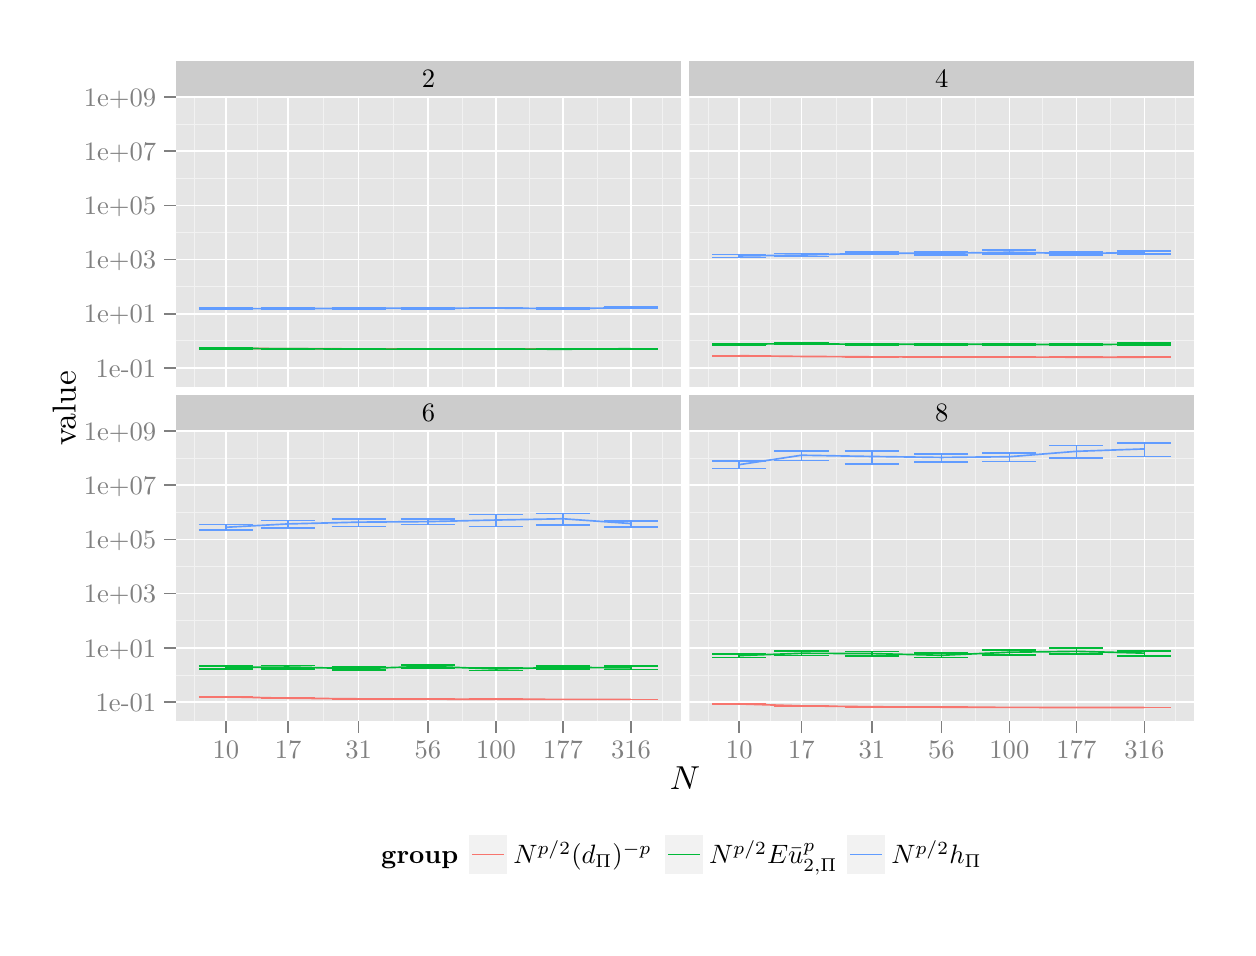
\begin{tikzpicture}[x=1pt,y=1pt]
\definecolor[named]{fillColor}{rgb}{1.00,1.00,1.00}
\path[use as bounding box,fill=fillColor,fill opacity=0.00] (0,0) rectangle (433.62,325.21);
\begin{scope}
\path[clip] (  0.00,  0.00) rectangle (433.62,325.21);
\definecolor[named]{drawColor}{rgb}{1.00,1.00,1.00}
\definecolor[named]{fillColor}{rgb}{1.00,1.00,1.00}

\path[draw=drawColor,line width= 0.6pt,line join=round,line cap=round,fill=fillColor] (  0.00,  0.00) rectangle (433.62,325.21);
\end{scope}
\begin{scope}
\path[clip] ( 53.55,195.47) rectangle (236.06,300.54);
\definecolor[named]{fillColor}{rgb}{0.90,0.90,0.90}

\path[fill=fillColor] ( 53.55,195.47) rectangle (236.06,300.54);
\definecolor[named]{drawColor}{rgb}{0.95,0.95,0.95}

\path[draw=drawColor,line width= 0.3pt,line join=round] ( 53.55,212.02) --
	(236.06,212.02);

\path[draw=drawColor,line width= 0.3pt,line join=round] ( 53.55,231.61) --
	(236.06,231.61);

\path[draw=drawColor,line width= 0.3pt,line join=round] ( 53.55,251.20) --
	(236.06,251.20);

\path[draw=drawColor,line width= 0.3pt,line join=round] ( 53.55,270.80) --
	(236.06,270.80);

\path[draw=drawColor,line width= 0.3pt,line join=round] ( 53.55,290.39) --
	(236.06,290.39);

\path[draw=drawColor,line width= 0.3pt,line join=round] ( 60.36,195.47) --
	( 60.36,300.54);

\path[draw=drawColor,line width= 0.3pt,line join=round] ( 82.85,195.47) --
	( 82.85,300.54);

\path[draw=drawColor,line width= 0.3pt,line join=round] (106.84,195.47) --
	(106.84,300.54);

\path[draw=drawColor,line width= 0.3pt,line join=round] (132.11,195.47) --
	(132.11,300.54);

\path[draw=drawColor,line width= 0.3pt,line join=round] (156.93,195.47) --
	(156.93,300.54);

\path[draw=drawColor,line width= 0.3pt,line join=round] (181.33,195.47) --
	(181.33,300.54);

\path[draw=drawColor,line width= 0.3pt,line join=round] (205.71,195.47) --
	(205.71,300.54);

\path[draw=drawColor,line width= 0.3pt,line join=round] (229.25,195.47) --
	(229.25,300.54);
\definecolor[named]{drawColor}{rgb}{1.00,1.00,1.00}

\path[draw=drawColor,line width= 0.6pt,line join=round] ( 53.55,202.22) --
	(236.06,202.22);

\path[draw=drawColor,line width= 0.6pt,line join=round] ( 53.55,221.81) --
	(236.06,221.81);

\path[draw=drawColor,line width= 0.6pt,line join=round] ( 53.55,241.41) --
	(236.06,241.41);

\path[draw=drawColor,line width= 0.6pt,line join=round] ( 53.55,261.00) --
	(236.06,261.00);

\path[draw=drawColor,line width= 0.6pt,line join=round] ( 53.55,280.59) --
	(236.06,280.59);

\path[draw=drawColor,line width= 0.6pt,line join=round] ( 53.55,300.19) --
	(236.06,300.19);

\path[draw=drawColor,line width= 0.6pt,line join=round] ( 71.61,195.47) --
	( 71.61,300.54);

\path[draw=drawColor,line width= 0.6pt,line join=round] ( 94.10,195.47) --
	( 94.10,300.54);

\path[draw=drawColor,line width= 0.6pt,line join=round] (119.57,195.47) --
	(119.57,300.54);

\path[draw=drawColor,line width= 0.6pt,line join=round] (144.64,195.47) --
	(144.64,300.54);

\path[draw=drawColor,line width= 0.6pt,line join=round] (169.22,195.47) --
	(169.22,300.54);

\path[draw=drawColor,line width= 0.6pt,line join=round] (193.43,195.47) --
	(193.43,300.54);

\path[draw=drawColor,line width= 0.6pt,line join=round] (218.00,195.47) --
	(218.00,300.54);
\definecolor[named]{drawColor}{rgb}{0.97,0.46,0.43}

\path[draw=drawColor,line width= 0.6pt,line join=round] ( 71.61,209.33) --
	( 94.10,209.21) --
	(119.57,209.14) --
	(144.64,209.11) --
	(169.22,209.09) --
	(193.43,209.08) --
	(218.00,209.07);
\definecolor[named]{drawColor}{rgb}{0.00,0.73,0.22}

\path[draw=drawColor,line width= 0.6pt,line join=round] ( 71.61,209.30) --
	( 94.10,209.20) --
	(119.57,209.05) --
	(144.64,209.08) --
	(169.22,209.11) --
	(193.43,209.01) --
	(218.00,209.19);
\definecolor[named]{drawColor}{rgb}{0.38,0.61,1.00}

\path[draw=drawColor,line width= 0.6pt,line join=round] ( 71.61,223.69) --
	( 94.10,223.69) --
	(119.57,223.78) --
	(144.64,223.83) --
	(169.22,223.87) --
	(193.43,223.71) --
	(218.00,224.00);
\definecolor[named]{drawColor}{rgb}{0.97,0.46,0.43}

\path[draw=drawColor,line width= 0.6pt,line join=round] ( 61.85,209.34) --
	( 81.37,209.34);

\path[draw=drawColor,line width= 0.6pt,line join=round] ( 71.61,209.34) --
	( 71.61,209.32);

\path[draw=drawColor,line width= 0.6pt,line join=round] ( 61.85,209.32) --
	( 81.37,209.32);

\path[draw=drawColor,line width= 0.6pt,line join=round] ( 84.34,209.21) --
	(103.86,209.21);

\path[draw=drawColor,line width= 0.6pt,line join=round] ( 94.10,209.21) --
	( 94.10,209.20);

\path[draw=drawColor,line width= 0.6pt,line join=round] ( 84.34,209.20) --
	(103.86,209.20);

\path[draw=drawColor,line width= 0.6pt,line join=round] (109.81,209.14) --
	(129.33,209.14);

\path[draw=drawColor,line width= 0.6pt,line join=round] (119.57,209.14) --
	(119.57,209.14);

\path[draw=drawColor,line width= 0.6pt,line join=round] (109.81,209.14) --
	(129.33,209.14);

\path[draw=drawColor,line width= 0.6pt,line join=round] (134.88,209.11) --
	(154.40,209.11);

\path[draw=drawColor,line width= 0.6pt,line join=round] (144.64,209.11) --
	(144.64,209.11);

\path[draw=drawColor,line width= 0.6pt,line join=round] (134.88,209.11) --
	(154.40,209.11);

\path[draw=drawColor,line width= 0.6pt,line join=round] (159.46,209.09) --
	(178.98,209.09);

\path[draw=drawColor,line width= 0.6pt,line join=round] (169.22,209.09) --
	(169.22,209.09);

\path[draw=drawColor,line width= 0.6pt,line join=round] (159.46,209.09) --
	(178.98,209.09);

\path[draw=drawColor,line width= 0.6pt,line join=round] (183.67,209.08) --
	(203.19,209.08);

\path[draw=drawColor,line width= 0.6pt,line join=round] (193.43,209.08) --
	(193.43,209.08);

\path[draw=drawColor,line width= 0.6pt,line join=round] (183.67,209.08) --
	(203.19,209.08);

\path[draw=drawColor,line width= 0.6pt,line join=round] (208.24,209.07) --
	(227.76,209.07);

\path[draw=drawColor,line width= 0.6pt,line join=round] (218.00,209.07) --
	(218.00,209.07);

\path[draw=drawColor,line width= 0.6pt,line join=round] (208.24,209.07) --
	(227.76,209.07);
\definecolor[named]{drawColor}{rgb}{0.00,0.73,0.22}

\path[draw=drawColor,line width= 0.6pt,line join=round] ( 61.85,209.41) --
	( 81.37,209.41);

\path[draw=drawColor,line width= 0.6pt,line join=round] ( 71.61,209.41) --
	( 71.61,209.19);

\path[draw=drawColor,line width= 0.6pt,line join=round] ( 61.85,209.19) --
	( 81.37,209.19);

\path[draw=drawColor,line width= 0.6pt,line join=round] ( 84.34,209.33) --
	(103.86,209.33);

\path[draw=drawColor,line width= 0.6pt,line join=round] ( 94.10,209.33) --
	( 94.10,209.09);

\path[draw=drawColor,line width= 0.6pt,line join=round] ( 84.34,209.09) --
	(103.86,209.09);

\path[draw=drawColor,line width= 0.6pt,line join=round] (109.81,209.16) --
	(129.33,209.16);

\path[draw=drawColor,line width= 0.6pt,line join=round] (119.57,209.16) --
	(119.57,208.93);

\path[draw=drawColor,line width= 0.6pt,line join=round] (109.81,208.93) --
	(129.33,208.93);

\path[draw=drawColor,line width= 0.6pt,line join=round] (134.88,209.20) --
	(154.40,209.20);

\path[draw=drawColor,line width= 0.6pt,line join=round] (144.64,209.20) --
	(144.64,208.97);

\path[draw=drawColor,line width= 0.6pt,line join=round] (134.88,208.97) --
	(154.40,208.97);

\path[draw=drawColor,line width= 0.6pt,line join=round] (159.46,209.22) --
	(178.98,209.22);

\path[draw=drawColor,line width= 0.6pt,line join=round] (169.22,209.22) --
	(169.22,208.99);

\path[draw=drawColor,line width= 0.6pt,line join=round] (159.46,208.99) --
	(178.98,208.99);

\path[draw=drawColor,line width= 0.6pt,line join=round] (183.67,209.13) --
	(203.19,209.13);

\path[draw=drawColor,line width= 0.6pt,line join=round] (193.43,209.13) --
	(193.43,208.90);

\path[draw=drawColor,line width= 0.6pt,line join=round] (183.67,208.90) --
	(203.19,208.90);

\path[draw=drawColor,line width= 0.6pt,line join=round] (208.24,209.31) --
	(227.76,209.31);

\path[draw=drawColor,line width= 0.6pt,line join=round] (218.00,209.31) --
	(218.00,209.07);

\path[draw=drawColor,line width= 0.6pt,line join=round] (208.24,209.07) --
	(227.76,209.07);
\definecolor[named]{drawColor}{rgb}{0.38,0.61,1.00}

\path[draw=drawColor,line width= 0.6pt,line join=round] ( 61.85,223.87) --
	( 81.37,223.87);

\path[draw=drawColor,line width= 0.6pt,line join=round] ( 71.61,223.87) --
	( 71.61,223.51);

\path[draw=drawColor,line width= 0.6pt,line join=round] ( 61.85,223.51) --
	( 81.37,223.51);

\path[draw=drawColor,line width= 0.6pt,line join=round] ( 84.34,223.88) --
	(103.86,223.88);

\path[draw=drawColor,line width= 0.6pt,line join=round] ( 94.10,223.88) --
	( 94.10,223.49);

\path[draw=drawColor,line width= 0.6pt,line join=round] ( 84.34,223.49) --
	(103.86,223.49);

\path[draw=drawColor,line width= 0.6pt,line join=round] (109.81,223.99) --
	(129.33,223.99);

\path[draw=drawColor,line width= 0.6pt,line join=round] (119.57,223.99) --
	(119.57,223.57);

\path[draw=drawColor,line width= 0.6pt,line join=round] (109.81,223.57) --
	(129.33,223.57);

\path[draw=drawColor,line width= 0.6pt,line join=round] (134.88,224.04) --
	(154.40,224.04);

\path[draw=drawColor,line width= 0.6pt,line join=round] (144.64,224.04) --
	(144.64,223.64);

\path[draw=drawColor,line width= 0.6pt,line join=round] (134.88,223.64) --
	(154.40,223.64);

\path[draw=drawColor,line width= 0.6pt,line join=round] (159.46,224.07) --
	(178.98,224.07);

\path[draw=drawColor,line width= 0.6pt,line join=round] (169.22,224.07) --
	(169.22,223.69);

\path[draw=drawColor,line width= 0.6pt,line join=round] (159.46,223.69) --
	(178.98,223.69);

\path[draw=drawColor,line width= 0.6pt,line join=round] (183.67,223.92) --
	(203.19,223.92);

\path[draw=drawColor,line width= 0.6pt,line join=round] (193.43,223.92) --
	(193.43,223.49);

\path[draw=drawColor,line width= 0.6pt,line join=round] (183.67,223.49) --
	(203.19,223.49);

\path[draw=drawColor,line width= 0.6pt,line join=round] (208.24,224.21) --
	(227.76,224.21);

\path[draw=drawColor,line width= 0.6pt,line join=round] (218.00,224.21) --
	(218.00,223.79);

\path[draw=drawColor,line width= 0.6pt,line join=round] (208.24,223.79) --
	(227.76,223.79);
\end{scope}
\begin{scope}
\path[clip] (239.07,195.47) rectangle (421.58,300.54);
\definecolor[named]{fillColor}{rgb}{0.90,0.90,0.90}

\path[fill=fillColor] (239.07,195.47) rectangle (421.57,300.54);
\definecolor[named]{drawColor}{rgb}{0.95,0.95,0.95}

\path[draw=drawColor,line width= 0.3pt,line join=round] (239.07,212.02) --
	(421.58,212.02);

\path[draw=drawColor,line width= 0.3pt,line join=round] (239.07,231.61) --
	(421.58,231.61);

\path[draw=drawColor,line width= 0.3pt,line join=round] (239.07,251.20) --
	(421.58,251.20);

\path[draw=drawColor,line width= 0.3pt,line join=round] (239.07,270.80) --
	(421.58,270.80);

\path[draw=drawColor,line width= 0.3pt,line join=round] (239.07,290.39) --
	(421.58,290.39);

\path[draw=drawColor,line width= 0.3pt,line join=round] (245.88,195.47) --
	(245.88,300.54);

\path[draw=drawColor,line width= 0.3pt,line join=round] (268.37,195.47) --
	(268.37,300.54);

\path[draw=drawColor,line width= 0.3pt,line join=round] (292.36,195.47) --
	(292.36,300.54);

\path[draw=drawColor,line width= 0.3pt,line join=round] (317.62,195.47) --
	(317.62,300.54);

\path[draw=drawColor,line width= 0.3pt,line join=round] (342.45,195.47) --
	(342.45,300.54);

\path[draw=drawColor,line width= 0.3pt,line join=round] (366.84,195.47) --
	(366.84,300.54);

\path[draw=drawColor,line width= 0.3pt,line join=round] (391.23,195.47) --
	(391.23,300.54);

\path[draw=drawColor,line width= 0.3pt,line join=round] (414.77,195.47) --
	(414.77,300.54);
\definecolor[named]{drawColor}{rgb}{1.00,1.00,1.00}

\path[draw=drawColor,line width= 0.6pt,line join=round] (239.07,202.22) --
	(421.58,202.22);

\path[draw=drawColor,line width= 0.6pt,line join=round] (239.07,221.81) --
	(421.58,221.81);

\path[draw=drawColor,line width= 0.6pt,line join=round] (239.07,241.41) --
	(421.58,241.41);

\path[draw=drawColor,line width= 0.6pt,line join=round] (239.07,261.00) --
	(421.58,261.00);

\path[draw=drawColor,line width= 0.6pt,line join=round] (239.07,280.59) --
	(421.58,280.59);

\path[draw=drawColor,line width= 0.6pt,line join=round] (239.07,300.19) --
	(421.58,300.19);

\path[draw=drawColor,line width= 0.6pt,line join=round] (257.13,195.47) --
	(257.13,300.54);

\path[draw=drawColor,line width= 0.6pt,line join=round] (279.62,195.47) --
	(279.62,300.54);

\path[draw=drawColor,line width= 0.6pt,line join=round] (305.09,195.47) --
	(305.09,300.54);

\path[draw=drawColor,line width= 0.6pt,line join=round] (330.16,195.47) --
	(330.16,300.54);

\path[draw=drawColor,line width= 0.6pt,line join=round] (354.74,195.47) --
	(354.74,300.54);

\path[draw=drawColor,line width= 0.6pt,line join=round] (378.95,195.47) --
	(378.95,300.54);

\path[draw=drawColor,line width= 0.6pt,line join=round] (403.52,195.47) --
	(403.52,300.54);
\definecolor[named]{drawColor}{rgb}{0.97,0.46,0.43}

\path[draw=drawColor,line width= 0.6pt,line join=round] (257.13,206.67) --
	(279.62,206.41) --
	(305.09,206.26) --
	(330.16,206.20) --
	(354.74,206.16) --
	(378.95,206.14) --
	(403.52,206.13);
\definecolor[named]{drawColor}{rgb}{0.00,0.73,0.22}

\path[draw=drawColor,line width= 0.6pt,line join=round] (257.13,210.90) --
	(279.62,210.97) --
	(305.09,210.79) --
	(330.16,210.82) --
	(354.74,210.83) --
	(378.95,210.61) --
	(403.52,210.88);
\definecolor[named]{drawColor}{rgb}{0.38,0.61,1.00}

\path[draw=drawColor,line width= 0.6pt,line join=round] (257.13,242.71) --
	(279.62,243.03) --
	(305.09,243.70) --
	(330.16,243.68) --
	(354.74,244.06) --
	(378.95,243.59) --
	(403.52,243.97);
\definecolor[named]{drawColor}{rgb}{0.97,0.46,0.43}

\path[draw=drawColor,line width= 0.6pt,line join=round] (247.36,206.69) --
	(266.89,206.69);

\path[draw=drawColor,line width= 0.6pt,line join=round] (257.13,206.69) --
	(257.13,206.65);

\path[draw=drawColor,line width= 0.6pt,line join=round] (247.36,206.65) --
	(266.89,206.65);

\path[draw=drawColor,line width= 0.6pt,line join=round] (269.86,206.42) --
	(289.38,206.42);

\path[draw=drawColor,line width= 0.6pt,line join=round] (279.62,206.42) --
	(279.62,206.40);

\path[draw=drawColor,line width= 0.6pt,line join=round] (269.86,206.40) --
	(289.38,206.40);

\path[draw=drawColor,line width= 0.6pt,line join=round] (295.33,206.27) --
	(314.85,206.27);

\path[draw=drawColor,line width= 0.6pt,line join=round] (305.09,206.27) --
	(305.09,206.26);

\path[draw=drawColor,line width= 0.6pt,line join=round] (295.33,206.26) --
	(314.85,206.26);

\path[draw=drawColor,line width= 0.6pt,line join=round] (320.40,206.20) --
	(339.92,206.20);

\path[draw=drawColor,line width= 0.6pt,line join=round] (330.16,206.20) --
	(330.16,206.20);

\path[draw=drawColor,line width= 0.6pt,line join=round] (320.40,206.20) --
	(339.92,206.20);

\path[draw=drawColor,line width= 0.6pt,line join=round] (344.98,206.16) --
	(364.50,206.16);

\path[draw=drawColor,line width= 0.6pt,line join=round] (354.74,206.16) --
	(354.74,206.16);

\path[draw=drawColor,line width= 0.6pt,line join=round] (344.98,206.16) --
	(364.50,206.16);

\path[draw=drawColor,line width= 0.6pt,line join=round] (369.19,206.14) --
	(388.71,206.14);

\path[draw=drawColor,line width= 0.6pt,line join=round] (378.95,206.14) --
	(378.95,206.14);

\path[draw=drawColor,line width= 0.6pt,line join=round] (369.19,206.14) --
	(388.71,206.14);

\path[draw=drawColor,line width= 0.6pt,line join=round] (393.76,206.13) --
	(413.28,206.13);

\path[draw=drawColor,line width= 0.6pt,line join=round] (403.52,206.13) --
	(403.52,206.13);

\path[draw=drawColor,line width= 0.6pt,line join=round] (393.76,206.13) --
	(413.28,206.13);
\definecolor[named]{drawColor}{rgb}{0.00,0.73,0.22}

\path[draw=drawColor,line width= 0.6pt,line join=round] (247.36,211.12) --
	(266.89,211.12);

\path[draw=drawColor,line width= 0.6pt,line join=round] (257.13,211.12) --
	(257.13,210.66);

\path[draw=drawColor,line width= 0.6pt,line join=round] (247.36,210.66) --
	(266.89,210.66);

\path[draw=drawColor,line width= 0.6pt,line join=round] (269.86,211.21) --
	(289.38,211.21);

\path[draw=drawColor,line width= 0.6pt,line join=round] (279.62,211.21) --
	(279.62,210.70);

\path[draw=drawColor,line width= 0.6pt,line join=round] (269.86,210.70) --
	(289.38,210.70);

\path[draw=drawColor,line width= 0.6pt,line join=round] (295.33,211.04) --
	(314.85,211.04);

\path[draw=drawColor,line width= 0.6pt,line join=round] (305.09,211.04) --
	(305.09,210.51);

\path[draw=drawColor,line width= 0.6pt,line join=round] (295.33,210.51) --
	(314.85,210.51);

\path[draw=drawColor,line width= 0.6pt,line join=round] (320.40,211.08) --
	(339.92,211.08);

\path[draw=drawColor,line width= 0.6pt,line join=round] (330.16,211.08) --
	(330.16,210.57);

\path[draw=drawColor,line width= 0.6pt,line join=round] (320.40,210.57) --
	(339.92,210.57);

\path[draw=drawColor,line width= 0.6pt,line join=round] (344.98,211.09) --
	(364.50,211.09);

\path[draw=drawColor,line width= 0.6pt,line join=round] (354.74,211.09) --
	(354.74,210.57);

\path[draw=drawColor,line width= 0.6pt,line join=round] (344.98,210.57) --
	(364.50,210.57);

\path[draw=drawColor,line width= 0.6pt,line join=round] (369.19,210.89) --
	(388.71,210.89);

\path[draw=drawColor,line width= 0.6pt,line join=round] (378.95,210.89) --
	(378.95,210.32);

\path[draw=drawColor,line width= 0.6pt,line join=round] (369.19,210.32) --
	(388.71,210.32);

\path[draw=drawColor,line width= 0.6pt,line join=round] (393.76,211.15) --
	(413.28,211.15);

\path[draw=drawColor,line width= 0.6pt,line join=round] (403.52,211.15) --
	(403.52,210.62);

\path[draw=drawColor,line width= 0.6pt,line join=round] (393.76,210.62) --
	(413.28,210.62);
\definecolor[named]{drawColor}{rgb}{0.38,0.61,1.00}

\path[draw=drawColor,line width= 0.6pt,line join=round] (247.36,243.21) --
	(266.89,243.21);

\path[draw=drawColor,line width= 0.6pt,line join=round] (257.13,243.21) --
	(257.13,242.20);

\path[draw=drawColor,line width= 0.6pt,line join=round] (247.36,242.20) --
	(266.89,242.20);

\path[draw=drawColor,line width= 0.6pt,line join=round] (269.86,243.60) --
	(289.38,243.60);

\path[draw=drawColor,line width= 0.6pt,line join=round] (279.62,243.60) --
	(279.62,242.48);

\path[draw=drawColor,line width= 0.6pt,line join=round] (269.86,242.48) --
	(289.38,242.48);

\path[draw=drawColor,line width= 0.6pt,line join=round] (295.33,244.20) --
	(314.85,244.20);

\path[draw=drawColor,line width= 0.6pt,line join=round] (305.09,244.20) --
	(305.09,243.20);

\path[draw=drawColor,line width= 0.6pt,line join=round] (295.33,243.20) --
	(314.85,243.20);

\path[draw=drawColor,line width= 0.6pt,line join=round] (320.40,244.26) --
	(339.92,244.26);

\path[draw=drawColor,line width= 0.6pt,line join=round] (330.16,244.26) --
	(330.16,243.09);

\path[draw=drawColor,line width= 0.6pt,line join=round] (320.40,243.09) --
	(339.92,243.09);

\path[draw=drawColor,line width= 0.6pt,line join=round] (344.98,244.82) --
	(364.50,244.82);

\path[draw=drawColor,line width= 0.6pt,line join=round] (354.74,244.82) --
	(354.74,243.34);

\path[draw=drawColor,line width= 0.6pt,line join=round] (344.98,243.34) --
	(364.50,243.34);

\path[draw=drawColor,line width= 0.6pt,line join=round] (369.19,244.12) --
	(388.71,244.12);

\path[draw=drawColor,line width= 0.6pt,line join=round] (378.95,244.12) --
	(378.95,243.04);

\path[draw=drawColor,line width= 0.6pt,line join=round] (369.19,243.04) --
	(388.71,243.04);

\path[draw=drawColor,line width= 0.6pt,line join=round] (393.76,244.58) --
	(413.28,244.58);

\path[draw=drawColor,line width= 0.6pt,line join=round] (403.52,244.58) --
	(403.52,243.33);

\path[draw=drawColor,line width= 0.6pt,line join=round] (393.76,243.33) --
	(413.28,243.33);
\end{scope}
\begin{scope}
\path[clip] ( 53.55, 74.76) rectangle (236.06,179.83);
\definecolor[named]{fillColor}{rgb}{0.90,0.90,0.90}

\path[fill=fillColor] ( 53.55, 74.76) rectangle (236.06,179.83);
\definecolor[named]{drawColor}{rgb}{0.95,0.95,0.95}

\path[draw=drawColor,line width= 0.3pt,line join=round] ( 53.55, 91.31) --
	(236.06, 91.31);

\path[draw=drawColor,line width= 0.3pt,line join=round] ( 53.55,110.90) --
	(236.06,110.90);

\path[draw=drawColor,line width= 0.3pt,line join=round] ( 53.55,130.49) --
	(236.06,130.49);

\path[draw=drawColor,line width= 0.3pt,line join=round] ( 53.55,150.09) --
	(236.06,150.09);

\path[draw=drawColor,line width= 0.3pt,line join=round] ( 53.55,169.68) --
	(236.06,169.68);

\path[draw=drawColor,line width= 0.3pt,line join=round] ( 60.36, 74.76) --
	( 60.36,179.83);

\path[draw=drawColor,line width= 0.3pt,line join=round] ( 82.85, 74.76) --
	( 82.85,179.83);

\path[draw=drawColor,line width= 0.3pt,line join=round] (106.84, 74.76) --
	(106.84,179.83);

\path[draw=drawColor,line width= 0.3pt,line join=round] (132.11, 74.76) --
	(132.11,179.83);

\path[draw=drawColor,line width= 0.3pt,line join=round] (156.93, 74.76) --
	(156.93,179.83);

\path[draw=drawColor,line width= 0.3pt,line join=round] (181.33, 74.76) --
	(181.33,179.83);

\path[draw=drawColor,line width= 0.3pt,line join=round] (205.71, 74.76) --
	(205.71,179.83);

\path[draw=drawColor,line width= 0.3pt,line join=round] (229.25, 74.76) --
	(229.25,179.83);
\definecolor[named]{drawColor}{rgb}{1.00,1.00,1.00}

\path[draw=drawColor,line width= 0.6pt,line join=round] ( 53.55, 81.51) --
	(236.06, 81.51);

\path[draw=drawColor,line width= 0.6pt,line join=round] ( 53.55,101.10) --
	(236.06,101.10);

\path[draw=drawColor,line width= 0.6pt,line join=round] ( 53.55,120.70) --
	(236.06,120.70);

\path[draw=drawColor,line width= 0.6pt,line join=round] ( 53.55,140.29) --
	(236.06,140.29);

\path[draw=drawColor,line width= 0.6pt,line join=round] ( 53.55,159.88) --
	(236.06,159.88);

\path[draw=drawColor,line width= 0.6pt,line join=round] ( 53.55,179.48) --
	(236.06,179.48);

\path[draw=drawColor,line width= 0.6pt,line join=round] ( 71.61, 74.76) --
	( 71.61,179.83);

\path[draw=drawColor,line width= 0.6pt,line join=round] ( 94.10, 74.76) --
	( 94.10,179.83);

\path[draw=drawColor,line width= 0.6pt,line join=round] (119.57, 74.76) --
	(119.57,179.83);

\path[draw=drawColor,line width= 0.6pt,line join=round] (144.64, 74.76) --
	(144.64,179.83);

\path[draw=drawColor,line width= 0.6pt,line join=round] (169.22, 74.76) --
	(169.22,179.83);

\path[draw=drawColor,line width= 0.6pt,line join=round] (193.43, 74.76) --
	(193.43,179.83);

\path[draw=drawColor,line width= 0.6pt,line join=round] (218.00, 74.76) --
	(218.00,179.83);
\definecolor[named]{drawColor}{rgb}{0.97,0.46,0.43}

\path[draw=drawColor,line width= 0.6pt,line join=round] ( 71.61, 83.41) --
	( 94.10, 82.91) --
	(119.57, 82.68) --
	(144.64, 82.58) --
	(169.22, 82.52) --
	(193.43, 82.50) --
	(218.00, 82.48);
\definecolor[named]{drawColor}{rgb}{0.00,0.73,0.22}

\path[draw=drawColor,line width= 0.6pt,line join=round] ( 71.61, 94.00) --
	( 94.10, 94.17) --
	(119.57, 93.60) --
	(144.64, 94.41) --
	(169.22, 93.48) --
	(193.43, 94.05) --
	(218.00, 93.88);
\definecolor[named]{drawColor}{rgb}{0.38,0.61,1.00}

\path[draw=drawColor,line width= 0.6pt,line join=round] ( 71.61,144.68) --
	( 94.10,145.89) --
	(119.57,146.53) --
	(144.64,146.73) --
	(169.22,147.29) --
	(193.43,147.75) --
	(218.00,146.02);
\definecolor[named]{drawColor}{rgb}{0.97,0.46,0.43}

\path[draw=drawColor,line width= 0.6pt,line join=round] ( 61.85, 83.46) --
	( 81.37, 83.46);

\path[draw=drawColor,line width= 0.6pt,line join=round] ( 71.61, 83.46) --
	( 71.61, 83.36);

\path[draw=drawColor,line width= 0.6pt,line join=round] ( 61.85, 83.36) --
	( 81.37, 83.36);

\path[draw=drawColor,line width= 0.6pt,line join=round] ( 84.34, 82.93) --
	(103.86, 82.93);

\path[draw=drawColor,line width= 0.6pt,line join=round] ( 94.10, 82.93) --
	( 94.10, 82.89);

\path[draw=drawColor,line width= 0.6pt,line join=round] ( 84.34, 82.89) --
	(103.86, 82.89);

\path[draw=drawColor,line width= 0.6pt,line join=round] (109.81, 82.69) --
	(129.33, 82.69);

\path[draw=drawColor,line width= 0.6pt,line join=round] (119.57, 82.69) --
	(119.57, 82.68);

\path[draw=drawColor,line width= 0.6pt,line join=round] (109.81, 82.68) --
	(129.33, 82.68);

\path[draw=drawColor,line width= 0.6pt,line join=round] (134.88, 82.59) --
	(154.40, 82.59);

\path[draw=drawColor,line width= 0.6pt,line join=round] (144.64, 82.59) --
	(144.64, 82.58);

\path[draw=drawColor,line width= 0.6pt,line join=round] (134.88, 82.58) --
	(154.40, 82.58);

\path[draw=drawColor,line width= 0.6pt,line join=round] (159.46, 82.52) --
	(178.98, 82.52);

\path[draw=drawColor,line width= 0.6pt,line join=round] (169.22, 82.52) --
	(169.22, 82.52);

\path[draw=drawColor,line width= 0.6pt,line join=round] (159.46, 82.52) --
	(178.98, 82.52);

\path[draw=drawColor,line width= 0.6pt,line join=round] (183.67, 82.50) --
	(203.19, 82.50);

\path[draw=drawColor,line width= 0.6pt,line join=round] (193.43, 82.50) --
	(193.43, 82.49);

\path[draw=drawColor,line width= 0.6pt,line join=round] (183.67, 82.49) --
	(203.19, 82.49);

\path[draw=drawColor,line width= 0.6pt,line join=round] (208.24, 82.48) --
	(227.76, 82.48);

\path[draw=drawColor,line width= 0.6pt,line join=round] (218.00, 82.48) --
	(218.00, 82.48);

\path[draw=drawColor,line width= 0.6pt,line join=round] (208.24, 82.48) --
	(227.76, 82.48);
\definecolor[named]{drawColor}{rgb}{0.00,0.73,0.22}

\path[draw=drawColor,line width= 0.6pt,line join=round] ( 61.85, 94.43) --
	( 81.37, 94.43);

\path[draw=drawColor,line width= 0.6pt,line join=round] ( 71.61, 94.43) --
	( 71.61, 93.57);

\path[draw=drawColor,line width= 0.6pt,line join=round] ( 61.85, 93.57) --
	( 81.37, 93.57);

\path[draw=drawColor,line width= 0.6pt,line join=round] ( 84.34, 94.79) --
	(103.86, 94.79);

\path[draw=drawColor,line width= 0.6pt,line join=round] ( 94.10, 94.79) --
	( 94.10, 93.52);

\path[draw=drawColor,line width= 0.6pt,line join=round] ( 84.34, 93.52) --
	(103.86, 93.52);

\path[draw=drawColor,line width= 0.6pt,line join=round] (109.81, 94.14) --
	(129.33, 94.14);

\path[draw=drawColor,line width= 0.6pt,line join=round] (119.57, 94.14) --
	(119.57, 93.13);

\path[draw=drawColor,line width= 0.6pt,line join=round] (109.81, 93.13) --
	(129.33, 93.13);

\path[draw=drawColor,line width= 0.6pt,line join=round] (134.88, 94.91) --
	(154.40, 94.91);

\path[draw=drawColor,line width= 0.6pt,line join=round] (144.64, 94.91) --
	(144.64, 93.89);

\path[draw=drawColor,line width= 0.6pt,line join=round] (134.88, 93.89) --
	(154.40, 93.89);

\path[draw=drawColor,line width= 0.6pt,line join=round] (159.46, 94.01) --
	(178.98, 94.01);

\path[draw=drawColor,line width= 0.6pt,line join=round] (169.22, 94.01) --
	(169.22, 92.93);

\path[draw=drawColor,line width= 0.6pt,line join=round] (159.46, 92.93) --
	(178.98, 92.93);

\path[draw=drawColor,line width= 0.6pt,line join=round] (183.67, 94.56) --
	(203.19, 94.56);

\path[draw=drawColor,line width= 0.6pt,line join=round] (193.43, 94.56) --
	(193.43, 93.54);

\path[draw=drawColor,line width= 0.6pt,line join=round] (183.67, 93.54) --
	(203.19, 93.54);

\path[draw=drawColor,line width= 0.6pt,line join=round] (208.24, 94.45) --
	(227.76, 94.45);

\path[draw=drawColor,line width= 0.6pt,line join=round] (218.00, 94.45) --
	(218.00, 93.31);

\path[draw=drawColor,line width= 0.6pt,line join=round] (208.24, 93.31) --
	(227.76, 93.31);
\definecolor[named]{drawColor}{rgb}{0.38,0.61,1.00}

\path[draw=drawColor,line width= 0.6pt,line join=round] ( 61.85,145.62) --
	( 81.37,145.62);

\path[draw=drawColor,line width= 0.6pt,line join=round] ( 71.61,145.62) --
	( 71.61,143.63);

\path[draw=drawColor,line width= 0.6pt,line join=round] ( 61.85,143.63) --
	( 81.37,143.63);

\path[draw=drawColor,line width= 0.6pt,line join=round] ( 84.34,147.14) --
	(103.86,147.14);

\path[draw=drawColor,line width= 0.6pt,line join=round] ( 94.10,147.14) --
	( 94.10,144.47);

\path[draw=drawColor,line width= 0.6pt,line join=round] ( 84.34,144.47) --
	(103.86,144.47);

\path[draw=drawColor,line width= 0.6pt,line join=round] (109.81,147.78) --
	(129.33,147.78);

\path[draw=drawColor,line width= 0.6pt,line join=round] (119.57,147.78) --
	(119.57,145.00);

\path[draw=drawColor,line width= 0.6pt,line join=round] (109.81,145.00) --
	(129.33,145.00);

\path[draw=drawColor,line width= 0.6pt,line join=round] (134.88,147.72) --
	(154.40,147.72);

\path[draw=drawColor,line width= 0.6pt,line join=round] (144.64,147.72) --
	(144.64,145.67);

\path[draw=drawColor,line width= 0.6pt,line join=round] (134.88,145.67) --
	(154.40,145.67);

\path[draw=drawColor,line width= 0.6pt,line join=round] (159.46,149.25) --
	(178.98,149.25);

\path[draw=drawColor,line width= 0.6pt,line join=round] (169.22,149.25) --
	(169.22,144.93);

\path[draw=drawColor,line width= 0.6pt,line join=round] (159.46,144.93) --
	(178.98,144.93);

\path[draw=drawColor,line width= 0.6pt,line join=round] (183.67,149.67) --
	(203.19,149.67);

\path[draw=drawColor,line width= 0.6pt,line join=round] (193.43,149.67) --
	(193.43,145.41);

\path[draw=drawColor,line width= 0.6pt,line join=round] (183.67,145.41) --
	(203.19,145.41);

\path[draw=drawColor,line width= 0.6pt,line join=round] (208.24,147.04) --
	(227.76,147.04);

\path[draw=drawColor,line width= 0.6pt,line join=round] (218.00,147.04) --
	(218.00,144.76);

\path[draw=drawColor,line width= 0.6pt,line join=round] (208.24,144.76) --
	(227.76,144.76);
\end{scope}
\begin{scope}
\path[clip] (239.07, 74.76) rectangle (421.58,179.83);
\definecolor[named]{fillColor}{rgb}{0.90,0.90,0.90}

\path[fill=fillColor] (239.07, 74.76) rectangle (421.57,179.83);
\definecolor[named]{drawColor}{rgb}{0.95,0.95,0.95}

\path[draw=drawColor,line width= 0.3pt,line join=round] (239.07, 91.31) --
	(421.58, 91.31);

\path[draw=drawColor,line width= 0.3pt,line join=round] (239.07,110.90) --
	(421.58,110.90);

\path[draw=drawColor,line width= 0.3pt,line join=round] (239.07,130.49) --
	(421.58,130.49);

\path[draw=drawColor,line width= 0.3pt,line join=round] (239.07,150.09) --
	(421.58,150.09);

\path[draw=drawColor,line width= 0.3pt,line join=round] (239.07,169.68) --
	(421.58,169.68);

\path[draw=drawColor,line width= 0.3pt,line join=round] (245.88, 74.76) --
	(245.88,179.83);

\path[draw=drawColor,line width= 0.3pt,line join=round] (268.37, 74.76) --
	(268.37,179.83);

\path[draw=drawColor,line width= 0.3pt,line join=round] (292.36, 74.76) --
	(292.36,179.83);

\path[draw=drawColor,line width= 0.3pt,line join=round] (317.62, 74.76) --
	(317.62,179.83);

\path[draw=drawColor,line width= 0.3pt,line join=round] (342.45, 74.76) --
	(342.45,179.83);

\path[draw=drawColor,line width= 0.3pt,line join=round] (366.84, 74.76) --
	(366.84,179.83);

\path[draw=drawColor,line width= 0.3pt,line join=round] (391.23, 74.76) --
	(391.23,179.83);

\path[draw=drawColor,line width= 0.3pt,line join=round] (414.77, 74.76) --
	(414.77,179.83);
\definecolor[named]{drawColor}{rgb}{1.00,1.00,1.00}

\path[draw=drawColor,line width= 0.6pt,line join=round] (239.07, 81.51) --
	(421.58, 81.51);

\path[draw=drawColor,line width= 0.6pt,line join=round] (239.07,101.10) --
	(421.58,101.10);

\path[draw=drawColor,line width= 0.6pt,line join=round] (239.07,120.70) --
	(421.58,120.70);

\path[draw=drawColor,line width= 0.6pt,line join=round] (239.07,140.29) --
	(421.58,140.29);

\path[draw=drawColor,line width= 0.6pt,line join=round] (239.07,159.88) --
	(421.58,159.88);

\path[draw=drawColor,line width= 0.6pt,line join=round] (239.07,179.48) --
	(421.58,179.48);

\path[draw=drawColor,line width= 0.6pt,line join=round] (257.13, 74.76) --
	(257.13,179.83);

\path[draw=drawColor,line width= 0.6pt,line join=round] (279.62, 74.76) --
	(279.62,179.83);

\path[draw=drawColor,line width= 0.6pt,line join=round] (305.09, 74.76) --
	(305.09,179.83);

\path[draw=drawColor,line width= 0.6pt,line join=round] (330.16, 74.76) --
	(330.16,179.83);

\path[draw=drawColor,line width= 0.6pt,line join=round] (354.74, 74.76) --
	(354.74,179.83);

\path[draw=drawColor,line width= 0.6pt,line join=round] (378.95, 74.76) --
	(378.95,179.83);

\path[draw=drawColor,line width= 0.6pt,line join=round] (403.52, 74.76) --
	(403.52,179.83);
\definecolor[named]{drawColor}{rgb}{0.97,0.46,0.43}

\path[draw=drawColor,line width= 0.6pt,line join=round] (257.13, 80.83) --
	(279.62, 80.14) --
	(305.09, 79.82) --
	(330.16, 79.67) --
	(354.74, 79.60) --
	(378.95, 79.56) --
	(403.52, 79.54);
\definecolor[named]{drawColor}{rgb}{0.00,0.73,0.22}

\path[draw=drawColor,line width= 0.6pt,line join=round] (257.13, 98.31) --
	(279.62, 99.14) --
	(305.09, 99.04) --
	(330.16, 98.42) --
	(354.74, 99.53) --
	(378.95, 99.85) --
	(403.52, 99.19);
\definecolor[named]{drawColor}{rgb}{0.38,0.61,1.00}

\path[draw=drawColor,line width= 0.6pt,line join=round] (257.13,167.31) --
	(279.62,170.71) --
	(305.09,170.26) --
	(330.16,169.91) --
	(354.74,170.17) --
	(378.95,172.12) --
	(403.52,172.99);
\definecolor[named]{drawColor}{rgb}{0.97,0.46,0.43}

\path[draw=drawColor,line width= 0.6pt,line join=round] (247.36, 80.89) --
	(266.89, 80.89);

\path[draw=drawColor,line width= 0.6pt,line join=round] (257.13, 80.89) --
	(257.13, 80.77);

\path[draw=drawColor,line width= 0.6pt,line join=round] (247.36, 80.77) --
	(266.89, 80.77);

\path[draw=drawColor,line width= 0.6pt,line join=round] (269.86, 80.17) --
	(289.38, 80.17);

\path[draw=drawColor,line width= 0.6pt,line join=round] (279.62, 80.17) --
	(279.62, 80.12);

\path[draw=drawColor,line width= 0.6pt,line join=round] (269.86, 80.12) --
	(289.38, 80.12);

\path[draw=drawColor,line width= 0.6pt,line join=round] (295.33, 79.83) --
	(314.85, 79.83);

\path[draw=drawColor,line width= 0.6pt,line join=round] (305.09, 79.83) --
	(305.09, 79.81);

\path[draw=drawColor,line width= 0.6pt,line join=round] (295.33, 79.81) --
	(314.85, 79.81);

\path[draw=drawColor,line width= 0.6pt,line join=round] (320.40, 79.67) --
	(339.92, 79.67);

\path[draw=drawColor,line width= 0.6pt,line join=round] (330.16, 79.67) --
	(330.16, 79.66);

\path[draw=drawColor,line width= 0.6pt,line join=round] (320.40, 79.66) --
	(339.92, 79.66);

\path[draw=drawColor,line width= 0.6pt,line join=round] (344.98, 79.60) --
	(364.50, 79.60);

\path[draw=drawColor,line width= 0.6pt,line join=round] (354.74, 79.60) --
	(354.74, 79.60);

\path[draw=drawColor,line width= 0.6pt,line join=round] (344.98, 79.60) --
	(364.50, 79.60);

\path[draw=drawColor,line width= 0.6pt,line join=round] (369.19, 79.56) --
	(388.71, 79.56);

\path[draw=drawColor,line width= 0.6pt,line join=round] (378.95, 79.56) --
	(378.95, 79.56);

\path[draw=drawColor,line width= 0.6pt,line join=round] (369.19, 79.56) --
	(388.71, 79.56);

\path[draw=drawColor,line width= 0.6pt,line join=round] (393.76, 79.54) --
	(413.28, 79.54);

\path[draw=drawColor,line width= 0.6pt,line join=round] (403.52, 79.54) --
	(403.52, 79.54);

\path[draw=drawColor,line width= 0.6pt,line join=round] (393.76, 79.54) --
	(413.28, 79.54);
\definecolor[named]{drawColor}{rgb}{0.00,0.73,0.22}

\path[draw=drawColor,line width= 0.6pt,line join=round] (247.36, 98.86) --
	(266.89, 98.86);

\path[draw=drawColor,line width= 0.6pt,line join=round] (257.13, 98.86) --
	(257.13, 97.68);

\path[draw=drawColor,line width= 0.6pt,line join=round] (247.36, 97.68) --
	(266.89, 97.68);

\path[draw=drawColor,line width= 0.6pt,line join=round] (269.86, 99.86) --
	(289.38, 99.86);

\path[draw=drawColor,line width= 0.6pt,line join=round] (279.62, 99.86) --
	(279.62, 98.34);

\path[draw=drawColor,line width= 0.6pt,line join=round] (269.86, 98.34) --
	(289.38, 98.34);

\path[draw=drawColor,line width= 0.6pt,line join=round] (295.33, 99.79) --
	(314.85, 99.79);

\path[draw=drawColor,line width= 0.6pt,line join=round] (305.09, 99.79) --
	(305.09, 98.23);

\path[draw=drawColor,line width= 0.6pt,line join=round] (295.33, 98.23) --
	(314.85, 98.23);

\path[draw=drawColor,line width= 0.6pt,line join=round] (320.40, 99.24) --
	(339.92, 99.24);

\path[draw=drawColor,line width= 0.6pt,line join=round] (330.16, 99.24) --
	(330.16, 97.63);

\path[draw=drawColor,line width= 0.6pt,line join=round] (320.40, 97.63) --
	(339.92, 97.63);

\path[draw=drawColor,line width= 0.6pt,line join=round] (344.98,100.40) --
	(364.50,100.40);

\path[draw=drawColor,line width= 0.6pt,line join=round] (354.74,100.40) --
	(354.74, 98.55);

\path[draw=drawColor,line width= 0.6pt,line join=round] (344.98, 98.55) --
	(364.50, 98.55);

\path[draw=drawColor,line width= 0.6pt,line join=round] (369.19,100.96) --
	(388.71,100.96);

\path[draw=drawColor,line width= 0.6pt,line join=round] (378.95,100.96) --
	(378.95, 98.78);

\path[draw=drawColor,line width= 0.6pt,line join=round] (369.19, 98.78) --
	(388.71, 98.78);

\path[draw=drawColor,line width= 0.6pt,line join=round] (393.76,100.04) --
	(413.28,100.04);

\path[draw=drawColor,line width= 0.6pt,line join=round] (403.52,100.04) --
	(403.52, 98.28);

\path[draw=drawColor,line width= 0.6pt,line join=round] (393.76, 98.28) --
	(413.28, 98.28);
\definecolor[named]{drawColor}{rgb}{0.38,0.61,1.00}

\path[draw=drawColor,line width= 0.6pt,line join=round] (247.36,168.61) --
	(266.89,168.61);

\path[draw=drawColor,line width= 0.6pt,line join=round] (257.13,168.61) --
	(257.13,165.91);

\path[draw=drawColor,line width= 0.6pt,line join=round] (247.36,165.91) --
	(266.89,165.91);

\path[draw=drawColor,line width= 0.6pt,line join=round] (269.86,172.26) --
	(289.38,172.26);

\path[draw=drawColor,line width= 0.6pt,line join=round] (279.62,172.26) --
	(279.62,168.84);

\path[draw=drawColor,line width= 0.6pt,line join=round] (269.86,168.84) --
	(289.38,168.84);

\path[draw=drawColor,line width= 0.6pt,line join=round] (295.33,172.33) --
	(314.85,172.33);

\path[draw=drawColor,line width= 0.6pt,line join=round] (305.09,172.33) --
	(305.09,167.61);

\path[draw=drawColor,line width= 0.6pt,line join=round] (295.33,167.61) --
	(314.85,167.61);

\path[draw=drawColor,line width= 0.6pt,line join=round] (320.40,171.20) --
	(339.92,171.20);

\path[draw=drawColor,line width= 0.6pt,line join=round] (330.16,171.20) --
	(330.16,168.37);

\path[draw=drawColor,line width= 0.6pt,line join=round] (320.40,168.37) --
	(339.92,168.37);

\path[draw=drawColor,line width= 0.6pt,line join=round] (344.98,171.54) --
	(364.50,171.54);

\path[draw=drawColor,line width= 0.6pt,line join=round] (354.74,171.54) --
	(354.74,168.45);

\path[draw=drawColor,line width= 0.6pt,line join=round] (344.98,168.45) --
	(364.50,168.45);

\path[draw=drawColor,line width= 0.6pt,line join=round] (369.19,174.17) --
	(388.71,174.17);

\path[draw=drawColor,line width= 0.6pt,line join=round] (378.95,174.17) --
	(378.95,169.71);

\path[draw=drawColor,line width= 0.6pt,line join=round] (369.19,169.71) --
	(388.71,169.71);

\path[draw=drawColor,line width= 0.6pt,line join=round] (393.76,175.05) --
	(413.28,175.05);

\path[draw=drawColor,line width= 0.6pt,line join=round] (403.52,175.05) --
	(403.52,170.30);

\path[draw=drawColor,line width= 0.6pt,line join=round] (393.76,170.30) --
	(413.28,170.30);
\end{scope}
\begin{scope}
\path[clip] (  0.00,  0.00) rectangle (433.62,325.21);
\definecolor[named]{fillColor}{rgb}{0.80,0.80,0.80}

\path[fill=fillColor] ( 53.55,300.54) rectangle (236.06,313.17);
\definecolor[named]{drawColor}{rgb}{0.00,0.00,0.00}

\node[text=drawColor,anchor=base,inner sep=0pt, outer sep=0pt, scale=  0.96] at (144.80,303.55) {2};
\end{scope}
\begin{scope}
\path[clip] (  0.00,  0.00) rectangle (433.62,325.21);
\definecolor[named]{fillColor}{rgb}{0.80,0.80,0.80}

\path[fill=fillColor] (239.07,300.54) rectangle (421.57,313.17);
\definecolor[named]{drawColor}{rgb}{0.00,0.00,0.00}

\node[text=drawColor,anchor=base,inner sep=0pt, outer sep=0pt, scale=  0.96] at (330.32,303.55) {4};
\end{scope}
\begin{scope}
\path[clip] (  0.00,  0.00) rectangle (433.62,325.21);
\definecolor[named]{fillColor}{rgb}{0.80,0.80,0.80}

\path[fill=fillColor] ( 53.55,179.83) rectangle (236.06,192.46);
\definecolor[named]{drawColor}{rgb}{0.00,0.00,0.00}

\node[text=drawColor,anchor=base,inner sep=0pt, outer sep=0pt, scale=  0.96] at (144.80,182.84) {6};
\end{scope}
\begin{scope}
\path[clip] (  0.00,  0.00) rectangle (433.62,325.21);
\definecolor[named]{fillColor}{rgb}{0.80,0.80,0.80}

\path[fill=fillColor] (239.07,179.83) rectangle (421.57,192.46);
\definecolor[named]{drawColor}{rgb}{0.00,0.00,0.00}

\node[text=drawColor,anchor=base,inner sep=0pt, outer sep=0pt, scale=  0.96] at (330.32,182.84) {8};
\end{scope}
\begin{scope}
\path[clip] (  0.00,  0.00) rectangle (433.62,325.21);
\definecolor[named]{drawColor}{rgb}{0.50,0.50,0.50}

\node[text=drawColor,anchor=base east,inner sep=0pt, outer sep=0pt, scale=  0.96] at ( 46.44,198.91) {1e-01};

\node[text=drawColor,anchor=base east,inner sep=0pt, outer sep=0pt, scale=  0.96] at ( 46.44,218.51) {1e+01};

\node[text=drawColor,anchor=base east,inner sep=0pt, outer sep=0pt, scale=  0.96] at ( 46.44,238.10) {1e+03};

\node[text=drawColor,anchor=base east,inner sep=0pt, outer sep=0pt, scale=  0.96] at ( 46.44,257.69) {1e+05};

\node[text=drawColor,anchor=base east,inner sep=0pt, outer sep=0pt, scale=  0.96] at ( 46.44,277.29) {1e+07};

\node[text=drawColor,anchor=base east,inner sep=0pt, outer sep=0pt, scale=  0.96] at ( 46.44,296.88) {1e+09};
\end{scope}
\begin{scope}
\path[clip] (  0.00,  0.00) rectangle (433.62,325.21);
\definecolor[named]{drawColor}{rgb}{0.50,0.50,0.50}

\path[draw=drawColor,line width= 0.6pt,line join=round] ( 49.28,202.22) --
	( 53.55,202.22);

\path[draw=drawColor,line width= 0.6pt,line join=round] ( 49.28,221.81) --
	( 53.55,221.81);

\path[draw=drawColor,line width= 0.6pt,line join=round] ( 49.28,241.41) --
	( 53.55,241.41);

\path[draw=drawColor,line width= 0.6pt,line join=round] ( 49.28,261.00) --
	( 53.55,261.00);

\path[draw=drawColor,line width= 0.6pt,line join=round] ( 49.28,280.59) --
	( 53.55,280.59);

\path[draw=drawColor,line width= 0.6pt,line join=round] ( 49.28,300.19) --
	( 53.55,300.19);
\end{scope}
\begin{scope}
\path[clip] (  0.00,  0.00) rectangle (433.62,325.21);
\definecolor[named]{drawColor}{rgb}{0.50,0.50,0.50}

\node[text=drawColor,anchor=base east,inner sep=0pt, outer sep=0pt, scale=  0.96] at ( 46.44, 78.20) {1e-01};

\node[text=drawColor,anchor=base east,inner sep=0pt, outer sep=0pt, scale=  0.96] at ( 46.44, 97.80) {1e+01};

\node[text=drawColor,anchor=base east,inner sep=0pt, outer sep=0pt, scale=  0.96] at ( 46.44,117.39) {1e+03};

\node[text=drawColor,anchor=base east,inner sep=0pt, outer sep=0pt, scale=  0.96] at ( 46.44,136.98) {1e+05};

\node[text=drawColor,anchor=base east,inner sep=0pt, outer sep=0pt, scale=  0.96] at ( 46.44,156.58) {1e+07};

\node[text=drawColor,anchor=base east,inner sep=0pt, outer sep=0pt, scale=  0.96] at ( 46.44,176.17) {1e+09};
\end{scope}
\begin{scope}
\path[clip] (  0.00,  0.00) rectangle (433.62,325.21);
\definecolor[named]{drawColor}{rgb}{0.50,0.50,0.50}

\path[draw=drawColor,line width= 0.6pt,line join=round] ( 49.28, 81.51) --
	( 53.55, 81.51);

\path[draw=drawColor,line width= 0.6pt,line join=round] ( 49.28,101.10) --
	( 53.55,101.10);

\path[draw=drawColor,line width= 0.6pt,line join=round] ( 49.28,120.70) --
	( 53.55,120.70);

\path[draw=drawColor,line width= 0.6pt,line join=round] ( 49.28,140.29) --
	( 53.55,140.29);

\path[draw=drawColor,line width= 0.6pt,line join=round] ( 49.28,159.88) --
	( 53.55,159.88);

\path[draw=drawColor,line width= 0.6pt,line join=round] ( 49.28,179.48) --
	( 53.55,179.48);
\end{scope}
\begin{scope}
\path[clip] (  0.00,  0.00) rectangle (433.62,325.21);
\definecolor[named]{drawColor}{rgb}{0.50,0.50,0.50}

\path[draw=drawColor,line width= 0.6pt,line join=round] ( 71.61, 70.49) --
	( 71.61, 74.76);

\path[draw=drawColor,line width= 0.6pt,line join=round] ( 94.10, 70.49) --
	( 94.10, 74.76);

\path[draw=drawColor,line width= 0.6pt,line join=round] (119.57, 70.49) --
	(119.57, 74.76);

\path[draw=drawColor,line width= 0.6pt,line join=round] (144.64, 70.49) --
	(144.64, 74.76);

\path[draw=drawColor,line width= 0.6pt,line join=round] (169.22, 70.49) --
	(169.22, 74.76);

\path[draw=drawColor,line width= 0.6pt,line join=round] (193.43, 70.49) --
	(193.43, 74.76);

\path[draw=drawColor,line width= 0.6pt,line join=round] (218.00, 70.49) --
	(218.00, 74.76);
\end{scope}
\begin{scope}
\path[clip] (  0.00,  0.00) rectangle (433.62,325.21);
\definecolor[named]{drawColor}{rgb}{0.50,0.50,0.50}

\node[text=drawColor,anchor=base,inner sep=0pt, outer sep=0pt, scale=  0.96] at ( 71.61, 61.03) {10};

\node[text=drawColor,anchor=base,inner sep=0pt, outer sep=0pt, scale=  0.96] at ( 94.10, 61.03) {17};

\node[text=drawColor,anchor=base,inner sep=0pt, outer sep=0pt, scale=  0.96] at (119.57, 61.03) {31};

\node[text=drawColor,anchor=base,inner sep=0pt, outer sep=0pt, scale=  0.96] at (144.64, 61.03) {56};

\node[text=drawColor,anchor=base,inner sep=0pt, outer sep=0pt, scale=  0.96] at (169.22, 61.03) {100};

\node[text=drawColor,anchor=base,inner sep=0pt, outer sep=0pt, scale=  0.96] at (193.43, 61.03) {177};

\node[text=drawColor,anchor=base,inner sep=0pt, outer sep=0pt, scale=  0.96] at (218.00, 61.03) {316};
\end{scope}
\begin{scope}
\path[clip] (  0.00,  0.00) rectangle (433.62,325.21);
\definecolor[named]{drawColor}{rgb}{0.50,0.50,0.50}

\path[draw=drawColor,line width= 0.6pt,line join=round] (257.13, 70.49) --
	(257.13, 74.76);

\path[draw=drawColor,line width= 0.6pt,line join=round] (279.62, 70.49) --
	(279.62, 74.76);

\path[draw=drawColor,line width= 0.6pt,line join=round] (305.09, 70.49) --
	(305.09, 74.76);

\path[draw=drawColor,line width= 0.6pt,line join=round] (330.16, 70.49) --
	(330.16, 74.76);

\path[draw=drawColor,line width= 0.6pt,line join=round] (354.74, 70.49) --
	(354.74, 74.76);

\path[draw=drawColor,line width= 0.6pt,line join=round] (378.95, 70.49) --
	(378.95, 74.76);

\path[draw=drawColor,line width= 0.6pt,line join=round] (403.52, 70.49) --
	(403.52, 74.76);
\end{scope}
\begin{scope}
\path[clip] (  0.00,  0.00) rectangle (433.62,325.21);
\definecolor[named]{drawColor}{rgb}{0.50,0.50,0.50}

\node[text=drawColor,anchor=base,inner sep=0pt, outer sep=0pt, scale=  0.96] at (257.13, 61.03) {10};

\node[text=drawColor,anchor=base,inner sep=0pt, outer sep=0pt, scale=  0.96] at (279.62, 61.03) {17};

\node[text=drawColor,anchor=base,inner sep=0pt, outer sep=0pt, scale=  0.96] at (305.09, 61.03) {31};

\node[text=drawColor,anchor=base,inner sep=0pt, outer sep=0pt, scale=  0.96] at (330.16, 61.03) {56};

\node[text=drawColor,anchor=base,inner sep=0pt, outer sep=0pt, scale=  0.96] at (354.74, 61.03) {100};

\node[text=drawColor,anchor=base,inner sep=0pt, outer sep=0pt, scale=  0.96] at (378.95, 61.03) {177};

\node[text=drawColor,anchor=base,inner sep=0pt, outer sep=0pt, scale=  0.96] at (403.52, 61.03) {316};
\end{scope}
\begin{scope}
\path[clip] (  0.00,  0.00) rectangle (433.62,325.21);
\definecolor[named]{drawColor}{rgb}{0.00,0.00,0.00}

\node[text=drawColor,anchor=base,inner sep=0pt, outer sep=0pt, scale=  1.20] at (237.56, 49.76) {$N$};
\end{scope}
\begin{scope}
\path[clip] (  0.00,  0.00) rectangle (433.62,325.21);
\definecolor[named]{drawColor}{rgb}{0.00,0.00,0.00}

\node[text=drawColor,rotate= 90.00,anchor=base,inner sep=0pt, outer sep=0pt, scale=  1.20] at ( 17.30,187.65) {value};
\end{scope}
\begin{scope}
\path[clip] (  0.00,  0.00) rectangle (433.62,325.21);
\definecolor[named]{fillColor}{rgb}{1.00,1.00,1.00}

\path[fill=fillColor] (123.49, 14.89) rectangle (351.63, 37.88);
\end{scope}
\begin{scope}
\path[clip] (  0.00,  0.00) rectangle (433.62,325.21);
\definecolor[named]{drawColor}{rgb}{0.00,0.00,0.00}

\node[text=drawColor,anchor=base west,inner sep=0pt, outer sep=0pt, scale=  0.96] at (127.76, 23.07) {\bfseries group};
\end{scope}
\begin{scope}
\path[clip] (  0.00,  0.00) rectangle (433.62,325.21);
\definecolor[named]{drawColor}{rgb}{1.00,1.00,1.00}
\definecolor[named]{fillColor}{rgb}{0.95,0.95,0.95}

\path[draw=drawColor,line width= 0.6pt,line join=round,line cap=round,fill=fillColor] (159.22, 19.16) rectangle (173.68, 33.61);
\end{scope}
\begin{scope}
\path[clip] (  0.00,  0.00) rectangle (433.62,325.21);
\definecolor[named]{drawColor}{rgb}{0.97,0.46,0.43}

\path[draw=drawColor,line width= 0.6pt,line join=round] (160.67, 26.39) -- (172.23, 26.39);
\end{scope}
\begin{scope}
\path[clip] (  0.00,  0.00) rectangle (433.62,325.21);
\definecolor[named]{drawColor}{rgb}{0.97,0.46,0.43}

\path[draw=drawColor,line width= 0.6pt,line join=round] (160.67, 26.39) -- (172.23, 26.39);
\end{scope}
\begin{scope}
\path[clip] (  0.00,  0.00) rectangle (433.62,325.21);
\definecolor[named]{drawColor}{rgb}{1.00,1.00,1.00}
\definecolor[named]{fillColor}{rgb}{0.95,0.95,0.95}

\path[draw=drawColor,line width= 0.6pt,line join=round,line cap=round,fill=fillColor] (229.96, 19.16) rectangle (244.41, 33.61);
\end{scope}
\begin{scope}
\path[clip] (  0.00,  0.00) rectangle (433.62,325.21);
\definecolor[named]{drawColor}{rgb}{0.00,0.73,0.22}

\path[draw=drawColor,line width= 0.6pt,line join=round] (231.41, 26.39) -- (242.97, 26.39);
\end{scope}
\begin{scope}
\path[clip] (  0.00,  0.00) rectangle (433.62,325.21);
\definecolor[named]{drawColor}{rgb}{0.00,0.73,0.22}

\path[draw=drawColor,line width= 0.6pt,line join=round] (231.41, 26.39) -- (242.97, 26.39);
\end{scope}
\begin{scope}
\path[clip] (  0.00,  0.00) rectangle (433.62,325.21);
\definecolor[named]{drawColor}{rgb}{1.00,1.00,1.00}
\definecolor[named]{fillColor}{rgb}{0.95,0.95,0.95}

\path[draw=drawColor,line width= 0.6pt,line join=round,line cap=round,fill=fillColor] (295.80, 19.16) rectangle (310.26, 33.61);
\end{scope}
\begin{scope}
\path[clip] (  0.00,  0.00) rectangle (433.62,325.21);
\definecolor[named]{drawColor}{rgb}{0.38,0.61,1.00}

\path[draw=drawColor,line width= 0.6pt,line join=round] (297.25, 26.39) -- (308.81, 26.39);
\end{scope}
\begin{scope}
\path[clip] (  0.00,  0.00) rectangle (433.62,325.21);
\definecolor[named]{drawColor}{rgb}{0.38,0.61,1.00}

\path[draw=drawColor,line width= 0.6pt,line join=round] (297.25, 26.39) -- (308.81, 26.39);
\end{scope}
\begin{scope}
\path[clip] (  0.00,  0.00) rectangle (433.62,325.21);
\definecolor[named]{drawColor}{rgb}{0.00,0.00,0.00}

\node[text=drawColor,anchor=base west,inner sep=0pt, outer sep=0pt, scale=  0.96] at (175.48, 23.08) {$N^{p/2}(d_{\Pi})^{-p}\;$};
\end{scope}
\begin{scope}
\path[clip] (  0.00,  0.00) rectangle (433.62,325.21);
\definecolor[named]{drawColor}{rgb}{0.00,0.00,0.00}

\node[text=drawColor,anchor=base west,inner sep=0pt, outer sep=0pt, scale=  0.96] at (246.22, 23.08) {$N^{p/2}\mathbb{E} \bar{u}_{2, \Pi}^p \;$};
\end{scope}
\begin{scope}
\path[clip] (  0.00,  0.00) rectangle (433.62,325.21);
\definecolor[named]{drawColor}{rgb}{0.00,0.00,0.00}

\node[text=drawColor,anchor=base west,inner sep=0pt, outer sep=0pt, scale=  0.96] at (312.06, 23.08) {$N^{p/2}h_{\Pi}\;$};
\end{scope}
\end{tikzpicture}

  \caption{Log-log plots of values scaled by proven upper bounds of rates, faceted on $p$.}
\end{figure}
Due to the flatness of the curves, we conclude that the bounds we have
proved are of the correct rate.  In addition, we can observe the
behavior of the constants as functions of $p$.  For instance, our
$f_{c_3}(p)$ constant for $\E h_{\Pi}^p$ appears to be an exponential
function of $p$.
\clearpage

Here, to compute the corresponding ``prime'' random variables in the
coupled pair, in each permutation we pick a transposition uniformly at
random among transpositions that switch groups.

\begin{figure}[!ht]
  \centering
  % Created by tikzDevice version 0.6.2-92-0ad2792 on 2013-03-04 16:59:26
% !TEX encoding = UTF-8 Unicode
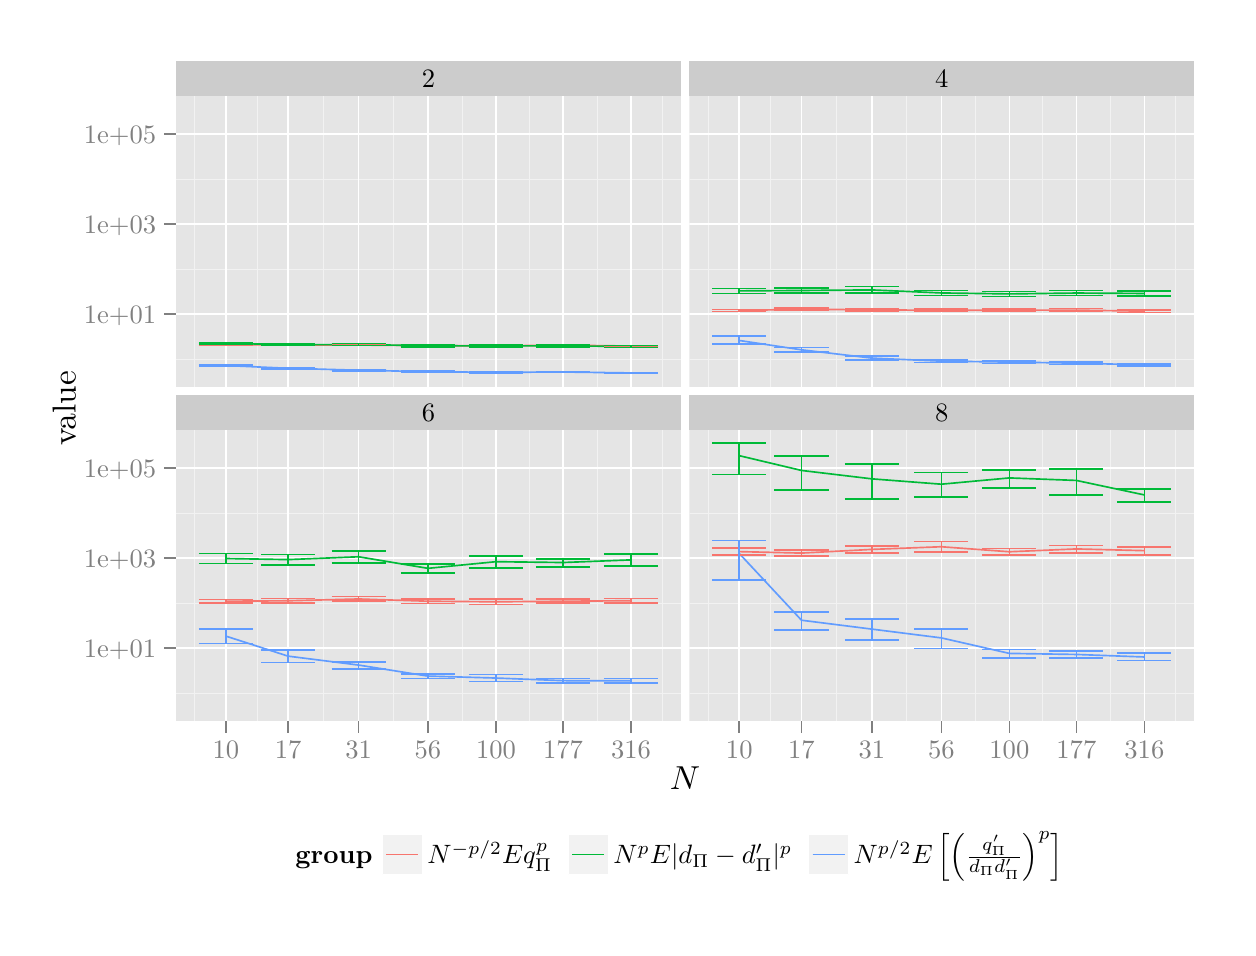
\begin{tikzpicture}[x=1pt,y=1pt]
\definecolor[named]{fillColor}{rgb}{1.00,1.00,1.00}
\path[use as bounding box,fill=fillColor,fill opacity=0.00] (0,0) rectangle (433.62,325.21);
\begin{scope}
\path[clip] (  0.00,  0.00) rectangle (433.62,325.21);
\definecolor[named]{drawColor}{rgb}{1.00,1.00,1.00}
\definecolor[named]{fillColor}{rgb}{1.00,1.00,1.00}

\path[draw=drawColor,line width= 0.6pt,line join=round,line cap=round,fill=fillColor] (  0.00,  0.00) rectangle (433.62,325.21);
\end{scope}
\begin{scope}
\path[clip] ( 53.55,195.47) rectangle (236.06,300.54);
\definecolor[named]{fillColor}{rgb}{0.90,0.90,0.90}

\path[fill=fillColor] ( 53.55,195.47) rectangle (236.06,300.54);
\definecolor[named]{drawColor}{rgb}{0.95,0.95,0.95}

\path[draw=drawColor,line width= 0.3pt,line join=round] ( 53.55,205.46) --
	(236.06,205.46);

\path[draw=drawColor,line width= 0.3pt,line join=round] ( 53.55,237.97) --
	(236.06,237.97);

\path[draw=drawColor,line width= 0.3pt,line join=round] ( 53.55,270.48) --
	(236.06,270.48);

\path[draw=drawColor,line width= 0.3pt,line join=round] ( 60.36,195.47) --
	( 60.36,300.54);

\path[draw=drawColor,line width= 0.3pt,line join=round] ( 82.85,195.47) --
	( 82.85,300.54);

\path[draw=drawColor,line width= 0.3pt,line join=round] (106.84,195.47) --
	(106.84,300.54);

\path[draw=drawColor,line width= 0.3pt,line join=round] (132.11,195.47) --
	(132.11,300.54);

\path[draw=drawColor,line width= 0.3pt,line join=round] (156.93,195.47) --
	(156.93,300.54);

\path[draw=drawColor,line width= 0.3pt,line join=round] (181.33,195.47) --
	(181.33,300.54);

\path[draw=drawColor,line width= 0.3pt,line join=round] (205.71,195.47) --
	(205.71,300.54);

\path[draw=drawColor,line width= 0.3pt,line join=round] (229.25,195.47) --
	(229.25,300.54);
\definecolor[named]{drawColor}{rgb}{1.00,1.00,1.00}

\path[draw=drawColor,line width= 0.6pt,line join=round] ( 53.55,221.71) --
	(236.06,221.71);

\path[draw=drawColor,line width= 0.6pt,line join=round] ( 53.55,254.22) --
	(236.06,254.22);

\path[draw=drawColor,line width= 0.6pt,line join=round] ( 53.55,286.73) --
	(236.06,286.73);

\path[draw=drawColor,line width= 0.6pt,line join=round] ( 71.61,195.47) --
	( 71.61,300.54);

\path[draw=drawColor,line width= 0.6pt,line join=round] ( 94.10,195.47) --
	( 94.10,300.54);

\path[draw=drawColor,line width= 0.6pt,line join=round] (119.57,195.47) --
	(119.57,300.54);

\path[draw=drawColor,line width= 0.6pt,line join=round] (144.64,195.47) --
	(144.64,300.54);

\path[draw=drawColor,line width= 0.6pt,line join=round] (169.22,195.47) --
	(169.22,300.54);

\path[draw=drawColor,line width= 0.6pt,line join=round] (193.43,195.47) --
	(193.43,300.54);

\path[draw=drawColor,line width= 0.6pt,line join=round] (218.00,195.47) --
	(218.00,300.54);
\definecolor[named]{drawColor}{rgb}{0.97,0.46,0.43}

\path[draw=drawColor,line width= 0.6pt,line join=round] ( 71.61,210.76) --
	( 94.10,210.52) --
	(119.57,210.52) --
	(144.64,210.30) --
	(169.22,210.22) --
	(193.43,210.48) --
	(218.00,210.17);
\definecolor[named]{drawColor}{rgb}{0.00,0.73,0.22}

\path[draw=drawColor,line width= 0.6pt,line join=round] ( 71.61,211.16) --
	( 94.10,210.65) --
	(119.57,210.71) --
	(144.64,210.28) --
	(169.22,210.19) --
	(193.43,210.25) --
	(218.00,209.99);
\definecolor[named]{drawColor}{rgb}{0.38,0.61,1.00}

\path[draw=drawColor,line width= 0.6pt,line join=round] ( 71.61,203.12) --
	( 94.10,202.13) --
	(119.57,201.43) --
	(144.64,200.89) --
	(169.22,200.66) --
	(193.43,200.78) --
	(218.00,200.45);
\definecolor[named]{drawColor}{rgb}{0.97,0.46,0.43}

\path[draw=drawColor,line width= 0.6pt,line join=round] ( 61.85,210.94) --
	( 81.37,210.94);

\path[draw=drawColor,line width= 0.6pt,line join=round] ( 71.61,210.94) --
	( 71.61,210.57);

\path[draw=drawColor,line width= 0.6pt,line join=round] ( 61.85,210.57) --
	( 81.37,210.57);

\path[draw=drawColor,line width= 0.6pt,line join=round] ( 84.34,210.70) --
	(103.86,210.70);

\path[draw=drawColor,line width= 0.6pt,line join=round] ( 94.10,210.70) --
	( 94.10,210.32);

\path[draw=drawColor,line width= 0.6pt,line join=round] ( 84.34,210.32) --
	(103.86,210.32);

\path[draw=drawColor,line width= 0.6pt,line join=round] (109.81,210.70) --
	(129.33,210.70);

\path[draw=drawColor,line width= 0.6pt,line join=round] (119.57,210.70) --
	(119.57,210.32);

\path[draw=drawColor,line width= 0.6pt,line join=round] (109.81,210.32) --
	(129.33,210.32);

\path[draw=drawColor,line width= 0.6pt,line join=round] (134.88,210.49) --
	(154.40,210.49);

\path[draw=drawColor,line width= 0.6pt,line join=round] (144.64,210.49) --
	(144.64,210.11);

\path[draw=drawColor,line width= 0.6pt,line join=round] (134.88,210.11) --
	(154.40,210.11);

\path[draw=drawColor,line width= 0.6pt,line join=round] (159.46,210.42) --
	(178.98,210.42);

\path[draw=drawColor,line width= 0.6pt,line join=round] (169.22,210.42) --
	(169.22,210.02);

\path[draw=drawColor,line width= 0.6pt,line join=round] (159.46,210.02) --
	(178.98,210.02);

\path[draw=drawColor,line width= 0.6pt,line join=round] (183.67,210.68) --
	(203.19,210.68);

\path[draw=drawColor,line width= 0.6pt,line join=round] (193.43,210.68) --
	(193.43,210.28);

\path[draw=drawColor,line width= 0.6pt,line join=round] (183.67,210.28) --
	(203.19,210.28);

\path[draw=drawColor,line width= 0.6pt,line join=round] (208.24,210.37) --
	(227.76,210.37);

\path[draw=drawColor,line width= 0.6pt,line join=round] (218.00,210.37) --
	(218.00,209.97);

\path[draw=drawColor,line width= 0.6pt,line join=round] (208.24,209.97) --
	(227.76,209.97);
\definecolor[named]{drawColor}{rgb}{0.00,0.73,0.22}

\path[draw=drawColor,line width= 0.6pt,line join=round] ( 61.85,211.50) --
	( 81.37,211.50);

\path[draw=drawColor,line width= 0.6pt,line join=round] ( 71.61,211.50) --
	( 71.61,210.83);

\path[draw=drawColor,line width= 0.6pt,line join=round] ( 61.85,210.83) --
	( 81.37,210.83);

\path[draw=drawColor,line width= 0.6pt,line join=round] ( 84.34,211.01) --
	(103.86,211.01);

\path[draw=drawColor,line width= 0.6pt,line join=round] ( 94.10,211.01) --
	( 94.10,210.32);

\path[draw=drawColor,line width= 0.6pt,line join=round] ( 84.34,210.32) --
	(103.86,210.32);

\path[draw=drawColor,line width= 0.6pt,line join=round] (109.81,211.09) --
	(129.33,211.09);

\path[draw=drawColor,line width= 0.6pt,line join=round] (119.57,211.09) --
	(119.57,210.33);

\path[draw=drawColor,line width= 0.6pt,line join=round] (109.81,210.33) --
	(129.33,210.33);

\path[draw=drawColor,line width= 0.6pt,line join=round] (134.88,210.61) --
	(154.40,210.61);

\path[draw=drawColor,line width= 0.6pt,line join=round] (144.64,210.61) --
	(144.64,209.93);

\path[draw=drawColor,line width= 0.6pt,line join=round] (134.88,209.93) --
	(154.40,209.93);

\path[draw=drawColor,line width= 0.6pt,line join=round] (159.46,210.53) --
	(178.98,210.53);

\path[draw=drawColor,line width= 0.6pt,line join=round] (169.22,210.53) --
	(169.22,209.85);

\path[draw=drawColor,line width= 0.6pt,line join=round] (159.46,209.85) --
	(178.98,209.85);

\path[draw=drawColor,line width= 0.6pt,line join=round] (183.67,210.60) --
	(203.19,210.60);

\path[draw=drawColor,line width= 0.6pt,line join=round] (193.43,210.60) --
	(193.43,209.92);

\path[draw=drawColor,line width= 0.6pt,line join=round] (183.67,209.92) --
	(203.19,209.92);

\path[draw=drawColor,line width= 0.6pt,line join=round] (208.24,210.30) --
	(227.76,210.30);

\path[draw=drawColor,line width= 0.6pt,line join=round] (218.00,210.30) --
	(218.00,209.65);

\path[draw=drawColor,line width= 0.6pt,line join=round] (208.24,209.65) --
	(227.76,209.65);
\definecolor[named]{drawColor}{rgb}{0.38,0.61,1.00}

\path[draw=drawColor,line width= 0.6pt,line join=round] ( 61.85,203.39) --
	( 81.37,203.39);

\path[draw=drawColor,line width= 0.6pt,line join=round] ( 71.61,203.39) --
	( 71.61,202.84);

\path[draw=drawColor,line width= 0.6pt,line join=round] ( 61.85,202.84) --
	( 81.37,202.84);

\path[draw=drawColor,line width= 0.6pt,line join=round] ( 84.34,202.37) --
	(103.86,202.37);

\path[draw=drawColor,line width= 0.6pt,line join=round] ( 94.10,202.37) --
	( 94.10,201.89);

\path[draw=drawColor,line width= 0.6pt,line join=round] ( 84.34,201.89) --
	(103.86,201.89);

\path[draw=drawColor,line width= 0.6pt,line join=round] (109.81,201.64) --
	(129.33,201.64);

\path[draw=drawColor,line width= 0.6pt,line join=round] (119.57,201.64) --
	(119.57,201.20);

\path[draw=drawColor,line width= 0.6pt,line join=round] (109.81,201.20) --
	(129.33,201.20);

\path[draw=drawColor,line width= 0.6pt,line join=round] (134.88,201.10) --
	(154.40,201.10);

\path[draw=drawColor,line width= 0.6pt,line join=round] (144.64,201.10) --
	(144.64,200.70);

\path[draw=drawColor,line width= 0.6pt,line join=round] (134.88,200.70) --
	(154.40,200.70);

\path[draw=drawColor,line width= 0.6pt,line join=round] (159.46,200.88) --
	(178.98,200.88);

\path[draw=drawColor,line width= 0.6pt,line join=round] (169.22,200.88) --
	(169.22,200.47);

\path[draw=drawColor,line width= 0.6pt,line join=round] (159.46,200.47) --
	(178.98,200.47);

\path[draw=drawColor,line width= 0.6pt,line join=round] (183.67,200.99) --
	(203.19,200.99);

\path[draw=drawColor,line width= 0.6pt,line join=round] (193.43,200.99) --
	(193.43,200.58);

\path[draw=drawColor,line width= 0.6pt,line join=round] (183.67,200.58) --
	(203.19,200.58);

\path[draw=drawColor,line width= 0.6pt,line join=round] (208.24,200.64) --
	(227.76,200.64);

\path[draw=drawColor,line width= 0.6pt,line join=round] (218.00,200.64) --
	(218.00,200.25);

\path[draw=drawColor,line width= 0.6pt,line join=round] (208.24,200.25) --
	(227.76,200.25);
\end{scope}
\begin{scope}
\path[clip] (239.07,195.47) rectangle (421.58,300.54);
\definecolor[named]{fillColor}{rgb}{0.90,0.90,0.90}

\path[fill=fillColor] (239.07,195.47) rectangle (421.57,300.54);
\definecolor[named]{drawColor}{rgb}{0.95,0.95,0.95}

\path[draw=drawColor,line width= 0.3pt,line join=round] (239.07,205.46) --
	(421.58,205.46);

\path[draw=drawColor,line width= 0.3pt,line join=round] (239.07,237.97) --
	(421.58,237.97);

\path[draw=drawColor,line width= 0.3pt,line join=round] (239.07,270.48) --
	(421.58,270.48);

\path[draw=drawColor,line width= 0.3pt,line join=round] (245.88,195.47) --
	(245.88,300.54);

\path[draw=drawColor,line width= 0.3pt,line join=round] (268.37,195.47) --
	(268.37,300.54);

\path[draw=drawColor,line width= 0.3pt,line join=round] (292.36,195.47) --
	(292.36,300.54);

\path[draw=drawColor,line width= 0.3pt,line join=round] (317.62,195.47) --
	(317.62,300.54);

\path[draw=drawColor,line width= 0.3pt,line join=round] (342.45,195.47) --
	(342.45,300.54);

\path[draw=drawColor,line width= 0.3pt,line join=round] (366.84,195.47) --
	(366.84,300.54);

\path[draw=drawColor,line width= 0.3pt,line join=round] (391.23,195.47) --
	(391.23,300.54);

\path[draw=drawColor,line width= 0.3pt,line join=round] (414.77,195.47) --
	(414.77,300.54);
\definecolor[named]{drawColor}{rgb}{1.00,1.00,1.00}

\path[draw=drawColor,line width= 0.6pt,line join=round] (239.07,221.71) --
	(421.58,221.71);

\path[draw=drawColor,line width= 0.6pt,line join=round] (239.07,254.22) --
	(421.58,254.22);

\path[draw=drawColor,line width= 0.6pt,line join=round] (239.07,286.73) --
	(421.58,286.73);

\path[draw=drawColor,line width= 0.6pt,line join=round] (257.13,195.47) --
	(257.13,300.54);

\path[draw=drawColor,line width= 0.6pt,line join=round] (279.62,195.47) --
	(279.62,300.54);

\path[draw=drawColor,line width= 0.6pt,line join=round] (305.09,195.47) --
	(305.09,300.54);

\path[draw=drawColor,line width= 0.6pt,line join=round] (330.16,195.47) --
	(330.16,300.54);

\path[draw=drawColor,line width= 0.6pt,line join=round] (354.74,195.47) --
	(354.74,300.54);

\path[draw=drawColor,line width= 0.6pt,line join=round] (378.95,195.47) --
	(378.95,300.54);

\path[draw=drawColor,line width= 0.6pt,line join=round] (403.52,195.47) --
	(403.52,300.54);
\definecolor[named]{drawColor}{rgb}{0.97,0.46,0.43}

\path[draw=drawColor,line width= 0.6pt,line join=round] (257.13,223.04) --
	(279.62,223.43) --
	(305.09,223.28) --
	(330.16,223.04) --
	(354.74,223.14) --
	(378.95,223.14) --
	(403.52,222.77);
\definecolor[named]{drawColor}{rgb}{0.00,0.73,0.22}

\path[draw=drawColor,line width= 0.6pt,line join=round] (257.13,230.10) --
	(279.62,230.24) --
	(305.09,230.44) --
	(330.16,229.35) --
	(354.74,229.00) --
	(378.95,229.32) --
	(403.52,229.16);
\definecolor[named]{drawColor}{rgb}{0.38,0.61,1.00}

\path[draw=drawColor,line width= 0.6pt,line join=round] (257.13,212.17) --
	(279.62,208.80) --
	(305.09,205.80) --
	(330.16,204.70) --
	(354.74,204.37) --
	(378.95,203.98) --
	(403.52,203.36);
\definecolor[named]{drawColor}{rgb}{0.97,0.46,0.43}

\path[draw=drawColor,line width= 0.6pt,line join=round] (247.36,223.40) --
	(266.89,223.40);

\path[draw=drawColor,line width= 0.6pt,line join=round] (257.13,223.40) --
	(257.13,222.64);

\path[draw=drawColor,line width= 0.6pt,line join=round] (247.36,222.64) --
	(266.89,222.64);

\path[draw=drawColor,line width= 0.6pt,line join=round] (269.86,223.86) --
	(289.38,223.86);

\path[draw=drawColor,line width= 0.6pt,line join=round] (279.62,223.86) --
	(279.62,222.99);

\path[draw=drawColor,line width= 0.6pt,line join=round] (269.86,222.99) --
	(289.38,222.99);

\path[draw=drawColor,line width= 0.6pt,line join=round] (295.33,223.73) --
	(314.85,223.73);

\path[draw=drawColor,line width= 0.6pt,line join=round] (305.09,223.73) --
	(305.09,222.84);

\path[draw=drawColor,line width= 0.6pt,line join=round] (295.33,222.84) --
	(314.85,222.84);

\path[draw=drawColor,line width= 0.6pt,line join=round] (320.40,223.48) --
	(339.92,223.48);

\path[draw=drawColor,line width= 0.6pt,line join=round] (330.16,223.48) --
	(330.16,222.60);

\path[draw=drawColor,line width= 0.6pt,line join=round] (320.40,222.60) --
	(339.92,222.60);

\path[draw=drawColor,line width= 0.6pt,line join=round] (344.98,223.56) --
	(364.50,223.56);

\path[draw=drawColor,line width= 0.6pt,line join=round] (354.74,223.56) --
	(354.74,222.68);

\path[draw=drawColor,line width= 0.6pt,line join=round] (344.98,222.68) --
	(364.50,222.68);

\path[draw=drawColor,line width= 0.6pt,line join=round] (369.19,223.67) --
	(388.71,223.67);

\path[draw=drawColor,line width= 0.6pt,line join=round] (378.95,223.67) --
	(378.95,222.63);

\path[draw=drawColor,line width= 0.6pt,line join=round] (369.19,222.63) --
	(388.71,222.63);

\path[draw=drawColor,line width= 0.6pt,line join=round] (393.76,223.21) --
	(413.28,223.21);

\path[draw=drawColor,line width= 0.6pt,line join=round] (403.52,223.21) --
	(403.52,222.31);

\path[draw=drawColor,line width= 0.6pt,line join=round] (393.76,222.31) --
	(413.28,222.31);
\definecolor[named]{drawColor}{rgb}{0.00,0.73,0.22}

\path[draw=drawColor,line width= 0.6pt,line join=round] (247.36,230.99) --
	(266.89,230.99);

\path[draw=drawColor,line width= 0.6pt,line join=round] (257.13,230.99) --
	(257.13,229.17);

\path[draw=drawColor,line width= 0.6pt,line join=round] (247.36,229.17) --
	(266.89,229.17);

\path[draw=drawColor,line width= 0.6pt,line join=round] (269.86,231.19) --
	(289.38,231.19);

\path[draw=drawColor,line width= 0.6pt,line join=round] (279.62,231.19) --
	(279.62,229.24);

\path[draw=drawColor,line width= 0.6pt,line join=round] (269.86,229.24) --
	(289.38,229.24);

\path[draw=drawColor,line width= 0.6pt,line join=round] (295.33,231.62) --
	(314.85,231.62);

\path[draw=drawColor,line width= 0.6pt,line join=round] (305.09,231.62) --
	(305.09,229.36);

\path[draw=drawColor,line width= 0.6pt,line join=round] (295.33,229.36) --
	(314.85,229.36);

\path[draw=drawColor,line width= 0.6pt,line join=round] (320.40,230.24) --
	(339.92,230.24);

\path[draw=drawColor,line width= 0.6pt,line join=round] (330.16,230.24) --
	(330.16,228.42);

\path[draw=drawColor,line width= 0.6pt,line join=round] (320.40,228.42) --
	(339.92,228.42);

\path[draw=drawColor,line width= 0.6pt,line join=round] (344.98,229.87) --
	(364.50,229.87);

\path[draw=drawColor,line width= 0.6pt,line join=round] (354.74,229.87) --
	(354.74,228.04);

\path[draw=drawColor,line width= 0.6pt,line join=round] (344.98,228.04) --
	(364.50,228.04);

\path[draw=drawColor,line width= 0.6pt,line join=round] (369.19,230.19) --
	(388.71,230.19);

\path[draw=drawColor,line width= 0.6pt,line join=round] (378.95,230.19) --
	(378.95,228.42);

\path[draw=drawColor,line width= 0.6pt,line join=round] (369.19,228.42) --
	(388.71,228.42);

\path[draw=drawColor,line width= 0.6pt,line join=round] (393.76,230.16) --
	(413.28,230.16);

\path[draw=drawColor,line width= 0.6pt,line join=round] (403.52,230.16) --
	(403.52,228.15);

\path[draw=drawColor,line width= 0.6pt,line join=round] (393.76,228.15) --
	(413.28,228.15);
\definecolor[named]{drawColor}{rgb}{0.38,0.61,1.00}

\path[draw=drawColor,line width= 0.6pt,line join=round] (247.36,213.71) --
	(266.89,213.71);

\path[draw=drawColor,line width= 0.6pt,line join=round] (257.13,213.71) --
	(257.13,210.81);

\path[draw=drawColor,line width= 0.6pt,line join=round] (247.36,210.81) --
	(266.89,210.81);

\path[draw=drawColor,line width= 0.6pt,line join=round] (269.86,209.64) --
	(289.38,209.64);

\path[draw=drawColor,line width= 0.6pt,line join=round] (279.62,209.64) --
	(279.62,207.91);

\path[draw=drawColor,line width= 0.6pt,line join=round] (269.86,207.91) --
	(289.38,207.91);

\path[draw=drawColor,line width= 0.6pt,line join=round] (295.33,206.45) --
	(314.85,206.45);

\path[draw=drawColor,line width= 0.6pt,line join=round] (305.09,206.45) --
	(305.09,205.14);

\path[draw=drawColor,line width= 0.6pt,line join=round] (295.33,205.14) --
	(314.85,205.14);

\path[draw=drawColor,line width= 0.6pt,line join=round] (320.40,205.18) --
	(339.92,205.18);

\path[draw=drawColor,line width= 0.6pt,line join=round] (330.16,205.18) --
	(330.16,204.24);

\path[draw=drawColor,line width= 0.6pt,line join=round] (320.40,204.24) --
	(339.92,204.24);

\path[draw=drawColor,line width= 0.6pt,line join=round] (344.98,204.87) --
	(364.50,204.87);

\path[draw=drawColor,line width= 0.6pt,line join=round] (354.74,204.87) --
	(354.74,203.84);

\path[draw=drawColor,line width= 0.6pt,line join=round] (344.98,203.84) --
	(364.50,203.84);

\path[draw=drawColor,line width= 0.6pt,line join=round] (369.19,204.46) --
	(388.71,204.46);

\path[draw=drawColor,line width= 0.6pt,line join=round] (378.95,204.46) --
	(378.95,203.44);

\path[draw=drawColor,line width= 0.6pt,line join=round] (369.19,203.44) --
	(388.71,203.44);

\path[draw=drawColor,line width= 0.6pt,line join=round] (393.76,203.79) --
	(413.28,203.79);

\path[draw=drawColor,line width= 0.6pt,line join=round] (403.52,203.79) --
	(403.52,202.91);

\path[draw=drawColor,line width= 0.6pt,line join=round] (393.76,202.91) --
	(413.28,202.91);
\end{scope}
\begin{scope}
\path[clip] ( 53.55, 74.76) rectangle (236.06,179.83);
\definecolor[named]{fillColor}{rgb}{0.90,0.90,0.90}

\path[fill=fillColor] ( 53.55, 74.76) rectangle (236.06,179.83);
\definecolor[named]{drawColor}{rgb}{0.95,0.95,0.95}

\path[draw=drawColor,line width= 0.3pt,line join=round] ( 53.55, 84.75) --
	(236.06, 84.75);

\path[draw=drawColor,line width= 0.3pt,line join=round] ( 53.55,117.26) --
	(236.06,117.26);

\path[draw=drawColor,line width= 0.3pt,line join=round] ( 53.55,149.77) --
	(236.06,149.77);

\path[draw=drawColor,line width= 0.3pt,line join=round] ( 60.36, 74.76) --
	( 60.36,179.83);

\path[draw=drawColor,line width= 0.3pt,line join=round] ( 82.85, 74.76) --
	( 82.85,179.83);

\path[draw=drawColor,line width= 0.3pt,line join=round] (106.84, 74.76) --
	(106.84,179.83);

\path[draw=drawColor,line width= 0.3pt,line join=round] (132.11, 74.76) --
	(132.11,179.83);

\path[draw=drawColor,line width= 0.3pt,line join=round] (156.93, 74.76) --
	(156.93,179.83);

\path[draw=drawColor,line width= 0.3pt,line join=round] (181.33, 74.76) --
	(181.33,179.83);

\path[draw=drawColor,line width= 0.3pt,line join=round] (205.71, 74.76) --
	(205.71,179.83);

\path[draw=drawColor,line width= 0.3pt,line join=round] (229.25, 74.76) --
	(229.25,179.83);
\definecolor[named]{drawColor}{rgb}{1.00,1.00,1.00}

\path[draw=drawColor,line width= 0.6pt,line join=round] ( 53.55,101.00) --
	(236.06,101.00);

\path[draw=drawColor,line width= 0.6pt,line join=round] ( 53.55,133.51) --
	(236.06,133.51);

\path[draw=drawColor,line width= 0.6pt,line join=round] ( 53.55,166.02) --
	(236.06,166.02);

\path[draw=drawColor,line width= 0.6pt,line join=round] ( 71.61, 74.76) --
	( 71.61,179.83);

\path[draw=drawColor,line width= 0.6pt,line join=round] ( 94.10, 74.76) --
	( 94.10,179.83);

\path[draw=drawColor,line width= 0.6pt,line join=round] (119.57, 74.76) --
	(119.57,179.83);

\path[draw=drawColor,line width= 0.6pt,line join=round] (144.64, 74.76) --
	(144.64,179.83);

\path[draw=drawColor,line width= 0.6pt,line join=round] (169.22, 74.76) --
	(169.22,179.83);

\path[draw=drawColor,line width= 0.6pt,line join=round] (193.43, 74.76) --
	(193.43,179.83);

\path[draw=drawColor,line width= 0.6pt,line join=round] (218.00, 74.76) --
	(218.00,179.83);
\definecolor[named]{drawColor}{rgb}{0.97,0.46,0.43}

\path[draw=drawColor,line width= 0.6pt,line join=round] ( 71.61,117.97) --
	( 94.10,118.11) --
	(119.57,118.77) --
	(144.64,117.96) --
	(169.22,117.74) --
	(193.43,117.96) --
	(218.00,118.14);
\definecolor[named]{drawColor}{rgb}{0.00,0.73,0.22}

\path[draw=drawColor,line width= 0.6pt,line join=round] ( 71.61,133.39) --
	( 94.10,133.00) --
	(119.57,134.02) --
	(144.64,129.84) --
	(169.22,132.24) --
	(193.43,131.94) --
	(218.00,132.89);
\definecolor[named]{drawColor}{rgb}{0.38,0.61,1.00}

\path[draw=drawColor,line width= 0.6pt,line join=round] ( 71.61,105.35) --
	( 94.10, 98.11) --
	(119.57, 94.89) --
	(144.64, 90.90) --
	(169.22, 90.20) --
	(193.43, 89.25) --
	(218.00, 89.21);
\definecolor[named]{drawColor}{rgb}{0.97,0.46,0.43}

\path[draw=drawColor,line width= 0.6pt,line join=round] ( 61.85,118.58) --
	( 81.37,118.58);

\path[draw=drawColor,line width= 0.6pt,line join=round] ( 71.61,118.58) --
	( 71.61,117.31);

\path[draw=drawColor,line width= 0.6pt,line join=round] ( 61.85,117.31) --
	( 81.37,117.31);

\path[draw=drawColor,line width= 0.6pt,line join=round] ( 84.34,118.95) --
	(103.86,118.95);

\path[draw=drawColor,line width= 0.6pt,line join=round] ( 94.10,118.95) --
	( 94.10,117.32);

\path[draw=drawColor,line width= 0.6pt,line join=round] ( 84.34,117.32) --
	(103.86,117.32);

\path[draw=drawColor,line width= 0.6pt,line join=round] (109.81,119.62) --
	(129.33,119.62);

\path[draw=drawColor,line width= 0.6pt,line join=round] (119.57,119.62) --
	(119.57,117.97);

\path[draw=drawColor,line width= 0.6pt,line join=round] (109.81,117.97) --
	(129.33,117.97);

\path[draw=drawColor,line width= 0.6pt,line join=round] (134.88,118.68) --
	(154.40,118.68);

\path[draw=drawColor,line width= 0.6pt,line join=round] (144.64,118.68) --
	(144.64,117.18);

\path[draw=drawColor,line width= 0.6pt,line join=round] (134.88,117.18) --
	(154.40,117.18);

\path[draw=drawColor,line width= 0.6pt,line join=round] (159.46,118.71) --
	(178.98,118.71);

\path[draw=drawColor,line width= 0.6pt,line join=round] (169.22,118.71) --
	(169.22,116.74);

\path[draw=drawColor,line width= 0.6pt,line join=round] (159.46,116.74) --
	(178.98,116.74);

\path[draw=drawColor,line width= 0.6pt,line join=round] (183.67,118.69) --
	(203.19,118.69);

\path[draw=drawColor,line width= 0.6pt,line join=round] (193.43,118.69) --
	(193.43,117.27);

\path[draw=drawColor,line width= 0.6pt,line join=round] (183.67,117.27) --
	(203.19,117.27);

\path[draw=drawColor,line width= 0.6pt,line join=round] (208.24,118.96) --
	(227.76,118.96);

\path[draw=drawColor,line width= 0.6pt,line join=round] (218.00,118.96) --
	(218.00,117.28);

\path[draw=drawColor,line width= 0.6pt,line join=round] (208.24,117.28) --
	(227.76,117.28);
\definecolor[named]{drawColor}{rgb}{0.00,0.73,0.22}

\path[draw=drawColor,line width= 0.6pt,line join=round] ( 61.85,135.16) --
	( 81.37,135.16);

\path[draw=drawColor,line width= 0.6pt,line join=round] ( 71.61,135.16) --
	( 71.61,131.61);

\path[draw=drawColor,line width= 0.6pt,line join=round] ( 61.85,131.61) --
	( 81.37,131.61);

\path[draw=drawColor,line width= 0.6pt,line join=round] ( 84.34,134.82) --
	(103.86,134.82);

\path[draw=drawColor,line width= 0.6pt,line join=round] ( 94.10,134.82) --
	( 94.10,131.02);

\path[draw=drawColor,line width= 0.6pt,line join=round] ( 84.34,131.02) --
	(103.86,131.02);

\path[draw=drawColor,line width= 0.6pt,line join=round] (109.81,136.21) --
	(129.33,136.21);

\path[draw=drawColor,line width= 0.6pt,line join=round] (119.57,136.21) --
	(119.57,131.81);

\path[draw=drawColor,line width= 0.6pt,line join=round] (109.81,131.81) --
	(129.33,131.81);

\path[draw=drawColor,line width= 0.6pt,line join=round] (134.88,131.35) --
	(154.40,131.35);

\path[draw=drawColor,line width= 0.6pt,line join=round] (144.64,131.35) --
	(144.64,128.04);

\path[draw=drawColor,line width= 0.6pt,line join=round] (134.88,128.04) --
	(154.40,128.04);

\path[draw=drawColor,line width= 0.6pt,line join=round] (159.46,134.30) --
	(178.98,134.30);

\path[draw=drawColor,line width= 0.6pt,line join=round] (169.22,134.30) --
	(169.22,129.92);

\path[draw=drawColor,line width= 0.6pt,line join=round] (159.46,129.92) --
	(178.98,129.92);

\path[draw=drawColor,line width= 0.6pt,line join=round] (183.67,133.31) --
	(203.19,133.31);

\path[draw=drawColor,line width= 0.6pt,line join=round] (193.43,133.31) --
	(193.43,130.33);

\path[draw=drawColor,line width= 0.6pt,line join=round] (183.67,130.33) --
	(203.19,130.33);

\path[draw=drawColor,line width= 0.6pt,line join=round] (208.24,134.93) --
	(227.76,134.93);

\path[draw=drawColor,line width= 0.6pt,line join=round] (218.00,134.93) --
	(218.00,130.63);

\path[draw=drawColor,line width= 0.6pt,line join=round] (208.24,130.63) --
	(227.76,130.63);
\definecolor[named]{drawColor}{rgb}{0.38,0.61,1.00}

\path[draw=drawColor,line width= 0.6pt,line join=round] ( 61.85,107.87) --
	( 81.37,107.87);

\path[draw=drawColor,line width= 0.6pt,line join=round] ( 71.61,107.87) --
	( 71.61,102.66);

\path[draw=drawColor,line width= 0.6pt,line join=round] ( 61.85,102.66) --
	( 81.37,102.66);

\path[draw=drawColor,line width= 0.6pt,line join=round] ( 84.34,100.29) --
	(103.86,100.29);

\path[draw=drawColor,line width= 0.6pt,line join=round] ( 94.10,100.29) --
	( 94.10, 95.86);

\path[draw=drawColor,line width= 0.6pt,line join=round] ( 84.34, 95.86) --
	(103.86, 95.86);

\path[draw=drawColor,line width= 0.6pt,line join=round] (109.81, 96.11) --
	(129.33, 96.11);

\path[draw=drawColor,line width= 0.6pt,line join=round] (119.57, 96.11) --
	(119.57, 93.56);

\path[draw=drawColor,line width= 0.6pt,line join=round] (109.81, 93.56) --
	(129.33, 93.56);

\path[draw=drawColor,line width= 0.6pt,line join=round] (134.88, 91.72) --
	(154.40, 91.72);

\path[draw=drawColor,line width= 0.6pt,line join=round] (144.64, 91.72) --
	(144.64, 90.03);

\path[draw=drawColor,line width= 0.6pt,line join=round] (134.88, 90.03) --
	(154.40, 90.03);

\path[draw=drawColor,line width= 0.6pt,line join=round] (159.46, 91.53) --
	(178.98, 91.53);

\path[draw=drawColor,line width= 0.6pt,line join=round] (169.22, 91.53) --
	(169.22, 88.97);

\path[draw=drawColor,line width= 0.6pt,line join=round] (159.46, 88.97) --
	(178.98, 88.97);

\path[draw=drawColor,line width= 0.6pt,line join=round] (183.67, 90.02) --
	(203.19, 90.02);

\path[draw=drawColor,line width= 0.6pt,line join=round] (193.43, 90.02) --
	(193.43, 88.46);

\path[draw=drawColor,line width= 0.6pt,line join=round] (183.67, 88.46) --
	(203.19, 88.46);

\path[draw=drawColor,line width= 0.6pt,line join=round] (208.24, 89.99) --
	(227.76, 89.99);

\path[draw=drawColor,line width= 0.6pt,line join=round] (218.00, 89.99) --
	(218.00, 88.37);

\path[draw=drawColor,line width= 0.6pt,line join=round] (208.24, 88.37) --
	(227.76, 88.37);
\end{scope}
\begin{scope}
\path[clip] (239.07, 74.76) rectangle (421.58,179.83);
\definecolor[named]{fillColor}{rgb}{0.90,0.90,0.90}

\path[fill=fillColor] (239.07, 74.76) rectangle (421.57,179.83);
\definecolor[named]{drawColor}{rgb}{0.95,0.95,0.95}

\path[draw=drawColor,line width= 0.3pt,line join=round] (239.07, 84.75) --
	(421.58, 84.75);

\path[draw=drawColor,line width= 0.3pt,line join=round] (239.07,117.26) --
	(421.58,117.26);

\path[draw=drawColor,line width= 0.3pt,line join=round] (239.07,149.77) --
	(421.58,149.77);

\path[draw=drawColor,line width= 0.3pt,line join=round] (245.88, 74.76) --
	(245.88,179.83);

\path[draw=drawColor,line width= 0.3pt,line join=round] (268.37, 74.76) --
	(268.37,179.83);

\path[draw=drawColor,line width= 0.3pt,line join=round] (292.36, 74.76) --
	(292.36,179.83);

\path[draw=drawColor,line width= 0.3pt,line join=round] (317.62, 74.76) --
	(317.62,179.83);

\path[draw=drawColor,line width= 0.3pt,line join=round] (342.45, 74.76) --
	(342.45,179.83);

\path[draw=drawColor,line width= 0.3pt,line join=round] (366.84, 74.76) --
	(366.84,179.83);

\path[draw=drawColor,line width= 0.3pt,line join=round] (391.23, 74.76) --
	(391.23,179.83);

\path[draw=drawColor,line width= 0.3pt,line join=round] (414.77, 74.76) --
	(414.77,179.83);
\definecolor[named]{drawColor}{rgb}{1.00,1.00,1.00}

\path[draw=drawColor,line width= 0.6pt,line join=round] (239.07,101.00) --
	(421.58,101.00);

\path[draw=drawColor,line width= 0.6pt,line join=round] (239.07,133.51) --
	(421.58,133.51);

\path[draw=drawColor,line width= 0.6pt,line join=round] (239.07,166.02) --
	(421.58,166.02);

\path[draw=drawColor,line width= 0.6pt,line join=round] (257.13, 74.76) --
	(257.13,179.83);

\path[draw=drawColor,line width= 0.6pt,line join=round] (279.62, 74.76) --
	(279.62,179.83);

\path[draw=drawColor,line width= 0.6pt,line join=round] (305.09, 74.76) --
	(305.09,179.83);

\path[draw=drawColor,line width= 0.6pt,line join=round] (330.16, 74.76) --
	(330.16,179.83);

\path[draw=drawColor,line width= 0.6pt,line join=round] (354.74, 74.76) --
	(354.74,179.83);

\path[draw=drawColor,line width= 0.6pt,line join=round] (378.95, 74.76) --
	(378.95,179.83);

\path[draw=drawColor,line width= 0.6pt,line join=round] (403.52, 74.76) --
	(403.52,179.83);
\definecolor[named]{drawColor}{rgb}{0.97,0.46,0.43}

\path[draw=drawColor,line width= 0.6pt,line join=round] (257.13,135.88) --
	(279.62,135.35) --
	(305.09,136.68) --
	(330.16,137.64) --
	(354.74,135.83) --
	(378.95,136.85) --
	(403.52,136.23);
\definecolor[named]{drawColor}{rgb}{0.00,0.73,0.22}

\path[draw=drawColor,line width= 0.6pt,line join=round] (257.13,170.55) --
	(279.62,165.21) --
	(305.09,162.17) --
	(330.16,160.24) --
	(354.74,162.51) --
	(378.95,161.60) --
	(403.52,156.36);
\definecolor[named]{drawColor}{rgb}{0.38,0.61,1.00}

\path[draw=drawColor,line width= 0.6pt,line join=round] (257.13,135.21) --
	(279.62,111.09) --
	(305.09,107.87) --
	(330.16,104.70) --
	(354.74, 99.10) --
	(378.95, 98.72) --
	(403.52, 97.81);
\definecolor[named]{drawColor}{rgb}{0.97,0.46,0.43}

\path[draw=drawColor,line width= 0.6pt,line join=round] (247.36,137.19) --
	(266.89,137.19);

\path[draw=drawColor,line width= 0.6pt,line join=round] (257.13,137.19) --
	(257.13,134.63);

\path[draw=drawColor,line width= 0.6pt,line join=round] (247.36,134.63) --
	(266.89,134.63);

\path[draw=drawColor,line width= 0.6pt,line join=round] (269.86,136.42) --
	(289.38,136.42);

\path[draw=drawColor,line width= 0.6pt,line join=round] (279.62,136.42) --
	(279.62,134.27);

\path[draw=drawColor,line width= 0.6pt,line join=round] (269.86,134.27) --
	(289.38,134.27);

\path[draw=drawColor,line width= 0.6pt,line join=round] (295.33,137.96) --
	(314.85,137.96);

\path[draw=drawColor,line width= 0.6pt,line join=round] (305.09,137.96) --
	(305.09,135.37);

\path[draw=drawColor,line width= 0.6pt,line join=round] (295.33,135.37) --
	(314.85,135.37);

\path[draw=drawColor,line width= 0.6pt,line join=round] (320.40,139.50) --
	(339.92,139.50);

\path[draw=drawColor,line width= 0.6pt,line join=round] (330.16,139.50) --
	(330.16,135.66);

\path[draw=drawColor,line width= 0.6pt,line join=round] (320.40,135.66) --
	(339.92,135.66);

\path[draw=drawColor,line width= 0.6pt,line join=round] (344.98,137.04) --
	(364.50,137.04);

\path[draw=drawColor,line width= 0.6pt,line join=round] (354.74,137.04) --
	(354.74,134.64);

\path[draw=drawColor,line width= 0.6pt,line join=round] (344.98,134.64) --
	(364.50,134.64);

\path[draw=drawColor,line width= 0.6pt,line join=round] (369.19,138.08) --
	(388.71,138.08);

\path[draw=drawColor,line width= 0.6pt,line join=round] (378.95,138.08) --
	(378.95,135.43);

\path[draw=drawColor,line width= 0.6pt,line join=round] (369.19,135.43) --
	(388.71,135.43);

\path[draw=drawColor,line width= 0.6pt,line join=round] (393.76,137.58) --
	(413.28,137.58);

\path[draw=drawColor,line width= 0.6pt,line join=round] (403.52,137.58) --
	(403.52,134.71);

\path[draw=drawColor,line width= 0.6pt,line join=round] (393.76,134.71) --
	(413.28,134.71);
\definecolor[named]{drawColor}{rgb}{0.00,0.73,0.22}

\path[draw=drawColor,line width= 0.6pt,line join=round] (247.36,175.05) --
	(266.89,175.05);

\path[draw=drawColor,line width= 0.6pt,line join=round] (257.13,175.05) --
	(257.13,163.72);

\path[draw=drawColor,line width= 0.6pt,line join=round] (247.36,163.72) --
	(266.89,163.72);

\path[draw=drawColor,line width= 0.6pt,line join=round] (269.86,170.55) --
	(289.38,170.55);

\path[draw=drawColor,line width= 0.6pt,line join=round] (279.62,170.55) --
	(279.62,158.24);

\path[draw=drawColor,line width= 0.6pt,line join=round] (269.86,158.24) --
	(289.38,158.24);

\path[draw=drawColor,line width= 0.6pt,line join=round] (295.33,167.49) --
	(314.85,167.49);

\path[draw=drawColor,line width= 0.6pt,line join=round] (305.09,167.49) --
	(305.09,154.91);

\path[draw=drawColor,line width= 0.6pt,line join=round] (295.33,154.91) --
	(314.85,154.91);

\path[draw=drawColor,line width= 0.6pt,line join=round] (320.40,164.53) --
	(339.92,164.53);

\path[draw=drawColor,line width= 0.6pt,line join=round] (330.16,164.53) --
	(330.16,155.59);

\path[draw=drawColor,line width= 0.6pt,line join=round] (320.40,155.59) --
	(339.92,155.59);

\path[draw=drawColor,line width= 0.6pt,line join=round] (344.98,165.44) --
	(364.50,165.44);

\path[draw=drawColor,line width= 0.6pt,line join=round] (354.74,165.44) --
	(354.74,158.84);

\path[draw=drawColor,line width= 0.6pt,line join=round] (344.98,158.84) --
	(364.50,158.84);

\path[draw=drawColor,line width= 0.6pt,line join=round] (369.19,165.78) --
	(388.71,165.78);

\path[draw=drawColor,line width= 0.6pt,line join=round] (378.95,165.78) --
	(378.95,156.30);

\path[draw=drawColor,line width= 0.6pt,line join=round] (369.19,156.30) --
	(388.71,156.30);

\path[draw=drawColor,line width= 0.6pt,line join=round] (393.76,158.60) --
	(413.28,158.60);

\path[draw=drawColor,line width= 0.6pt,line join=round] (403.52,158.60) --
	(403.52,153.74);

\path[draw=drawColor,line width= 0.6pt,line join=round] (393.76,153.74) --
	(413.28,153.74);
\definecolor[named]{drawColor}{rgb}{0.38,0.61,1.00}

\path[draw=drawColor,line width= 0.6pt,line join=round] (247.36,139.92) --
	(266.89,139.92);

\path[draw=drawColor,line width= 0.6pt,line join=round] (257.13,139.92) --
	(257.13,125.72);

\path[draw=drawColor,line width= 0.6pt,line join=round] (247.36,125.72) --
	(266.89,125.72);

\path[draw=drawColor,line width= 0.6pt,line join=round] (269.86,114.04) --
	(289.38,114.04);

\path[draw=drawColor,line width= 0.6pt,line join=round] (279.62,114.04) --
	(279.62,107.64);

\path[draw=drawColor,line width= 0.6pt,line join=round] (269.86,107.64) --
	(289.38,107.64);

\path[draw=drawColor,line width= 0.6pt,line join=round] (295.33,111.49) --
	(314.85,111.49);

\path[draw=drawColor,line width= 0.6pt,line join=round] (305.09,111.49) --
	(305.09,103.83);

\path[draw=drawColor,line width= 0.6pt,line join=round] (295.33,103.83) --
	(314.85,103.83);

\path[draw=drawColor,line width= 0.6pt,line join=round] (320.40,108.00) --
	(339.92,108.00);

\path[draw=drawColor,line width= 0.6pt,line join=round] (330.16,108.00) --
	(330.16,100.88);

\path[draw=drawColor,line width= 0.6pt,line join=round] (320.40,100.88) --
	(339.92,100.88);

\path[draw=drawColor,line width= 0.6pt,line join=round] (344.98,100.47) --
	(364.50,100.47);

\path[draw=drawColor,line width= 0.6pt,line join=round] (354.74,100.47) --
	(354.74, 97.49);

\path[draw=drawColor,line width= 0.6pt,line join=round] (344.98, 97.49) --
	(364.50, 97.49);

\path[draw=drawColor,line width= 0.6pt,line join=round] (369.19, 99.99) --
	(388.71, 99.99);

\path[draw=drawColor,line width= 0.6pt,line join=round] (378.95, 99.99) --
	(378.95, 97.41);

\path[draw=drawColor,line width= 0.6pt,line join=round] (369.19, 97.41) --
	(388.71, 97.41);

\path[draw=drawColor,line width= 0.6pt,line join=round] (393.76, 99.20) --
	(413.28, 99.20);

\path[draw=drawColor,line width= 0.6pt,line join=round] (403.52, 99.20) --
	(403.52, 96.49);

\path[draw=drawColor,line width= 0.6pt,line join=round] (393.76, 96.49) --
	(413.28, 96.49);
\end{scope}
\begin{scope}
\path[clip] (  0.00,  0.00) rectangle (433.62,325.21);
\definecolor[named]{fillColor}{rgb}{0.80,0.80,0.80}

\path[fill=fillColor] ( 53.55,300.54) rectangle (236.06,313.17);
\definecolor[named]{drawColor}{rgb}{0.00,0.00,0.00}

\node[text=drawColor,anchor=base,inner sep=0pt, outer sep=0pt, scale=  0.96] at (144.80,303.55) {2};
\end{scope}
\begin{scope}
\path[clip] (  0.00,  0.00) rectangle (433.62,325.21);
\definecolor[named]{fillColor}{rgb}{0.80,0.80,0.80}

\path[fill=fillColor] (239.07,300.54) rectangle (421.57,313.17);
\definecolor[named]{drawColor}{rgb}{0.00,0.00,0.00}

\node[text=drawColor,anchor=base,inner sep=0pt, outer sep=0pt, scale=  0.96] at (330.32,303.55) {4};
\end{scope}
\begin{scope}
\path[clip] (  0.00,  0.00) rectangle (433.62,325.21);
\definecolor[named]{fillColor}{rgb}{0.80,0.80,0.80}

\path[fill=fillColor] ( 53.55,179.83) rectangle (236.06,192.46);
\definecolor[named]{drawColor}{rgb}{0.00,0.00,0.00}

\node[text=drawColor,anchor=base,inner sep=0pt, outer sep=0pt, scale=  0.96] at (144.80,182.84) {6};
\end{scope}
\begin{scope}
\path[clip] (  0.00,  0.00) rectangle (433.62,325.21);
\definecolor[named]{fillColor}{rgb}{0.80,0.80,0.80}

\path[fill=fillColor] (239.07,179.83) rectangle (421.57,192.46);
\definecolor[named]{drawColor}{rgb}{0.00,0.00,0.00}

\node[text=drawColor,anchor=base,inner sep=0pt, outer sep=0pt, scale=  0.96] at (330.32,182.84) {8};
\end{scope}
\begin{scope}
\path[clip] (  0.00,  0.00) rectangle (433.62,325.21);
\definecolor[named]{drawColor}{rgb}{0.50,0.50,0.50}

\node[text=drawColor,anchor=base east,inner sep=0pt, outer sep=0pt, scale=  0.96] at ( 46.44,218.41) {1e+01};

\node[text=drawColor,anchor=base east,inner sep=0pt, outer sep=0pt, scale=  0.96] at ( 46.44,250.92) {1e+03};

\node[text=drawColor,anchor=base east,inner sep=0pt, outer sep=0pt, scale=  0.96] at ( 46.44,283.42) {1e+05};
\end{scope}
\begin{scope}
\path[clip] (  0.00,  0.00) rectangle (433.62,325.21);
\definecolor[named]{drawColor}{rgb}{0.50,0.50,0.50}

\path[draw=drawColor,line width= 0.6pt,line join=round] ( 49.28,221.71) --
	( 53.55,221.71);

\path[draw=drawColor,line width= 0.6pt,line join=round] ( 49.28,254.22) --
	( 53.55,254.22);

\path[draw=drawColor,line width= 0.6pt,line join=round] ( 49.28,286.73) --
	( 53.55,286.73);
\end{scope}
\begin{scope}
\path[clip] (  0.00,  0.00) rectangle (433.62,325.21);
\definecolor[named]{drawColor}{rgb}{0.50,0.50,0.50}

\node[text=drawColor,anchor=base east,inner sep=0pt, outer sep=0pt, scale=  0.96] at ( 46.44, 97.70) {1e+01};

\node[text=drawColor,anchor=base east,inner sep=0pt, outer sep=0pt, scale=  0.96] at ( 46.44,130.21) {1e+03};

\node[text=drawColor,anchor=base east,inner sep=0pt, outer sep=0pt, scale=  0.96] at ( 46.44,162.71) {1e+05};
\end{scope}
\begin{scope}
\path[clip] (  0.00,  0.00) rectangle (433.62,325.21);
\definecolor[named]{drawColor}{rgb}{0.50,0.50,0.50}

\path[draw=drawColor,line width= 0.6pt,line join=round] ( 49.28,101.00) --
	( 53.55,101.00);

\path[draw=drawColor,line width= 0.6pt,line join=round] ( 49.28,133.51) --
	( 53.55,133.51);

\path[draw=drawColor,line width= 0.6pt,line join=round] ( 49.28,166.02) --
	( 53.55,166.02);
\end{scope}
\begin{scope}
\path[clip] (  0.00,  0.00) rectangle (433.62,325.21);
\definecolor[named]{drawColor}{rgb}{0.50,0.50,0.50}

\path[draw=drawColor,line width= 0.6pt,line join=round] ( 71.61, 70.49) --
	( 71.61, 74.76);

\path[draw=drawColor,line width= 0.6pt,line join=round] ( 94.10, 70.49) --
	( 94.10, 74.76);

\path[draw=drawColor,line width= 0.6pt,line join=round] (119.57, 70.49) --
	(119.57, 74.76);

\path[draw=drawColor,line width= 0.6pt,line join=round] (144.64, 70.49) --
	(144.64, 74.76);

\path[draw=drawColor,line width= 0.6pt,line join=round] (169.22, 70.49) --
	(169.22, 74.76);

\path[draw=drawColor,line width= 0.6pt,line join=round] (193.43, 70.49) --
	(193.43, 74.76);

\path[draw=drawColor,line width= 0.6pt,line join=round] (218.00, 70.49) --
	(218.00, 74.76);
\end{scope}
\begin{scope}
\path[clip] (  0.00,  0.00) rectangle (433.62,325.21);
\definecolor[named]{drawColor}{rgb}{0.50,0.50,0.50}

\node[text=drawColor,anchor=base,inner sep=0pt, outer sep=0pt, scale=  0.96] at ( 71.61, 61.03) {10};

\node[text=drawColor,anchor=base,inner sep=0pt, outer sep=0pt, scale=  0.96] at ( 94.10, 61.03) {17};

\node[text=drawColor,anchor=base,inner sep=0pt, outer sep=0pt, scale=  0.96] at (119.57, 61.03) {31};

\node[text=drawColor,anchor=base,inner sep=0pt, outer sep=0pt, scale=  0.96] at (144.64, 61.03) {56};

\node[text=drawColor,anchor=base,inner sep=0pt, outer sep=0pt, scale=  0.96] at (169.22, 61.03) {100};

\node[text=drawColor,anchor=base,inner sep=0pt, outer sep=0pt, scale=  0.96] at (193.43, 61.03) {177};

\node[text=drawColor,anchor=base,inner sep=0pt, outer sep=0pt, scale=  0.96] at (218.00, 61.03) {316};
\end{scope}
\begin{scope}
\path[clip] (  0.00,  0.00) rectangle (433.62,325.21);
\definecolor[named]{drawColor}{rgb}{0.50,0.50,0.50}

\path[draw=drawColor,line width= 0.6pt,line join=round] (257.13, 70.49) --
	(257.13, 74.76);

\path[draw=drawColor,line width= 0.6pt,line join=round] (279.62, 70.49) --
	(279.62, 74.76);

\path[draw=drawColor,line width= 0.6pt,line join=round] (305.09, 70.49) --
	(305.09, 74.76);

\path[draw=drawColor,line width= 0.6pt,line join=round] (330.16, 70.49) --
	(330.16, 74.76);

\path[draw=drawColor,line width= 0.6pt,line join=round] (354.74, 70.49) --
	(354.74, 74.76);

\path[draw=drawColor,line width= 0.6pt,line join=round] (378.95, 70.49) --
	(378.95, 74.76);

\path[draw=drawColor,line width= 0.6pt,line join=round] (403.52, 70.49) --
	(403.52, 74.76);
\end{scope}
\begin{scope}
\path[clip] (  0.00,  0.00) rectangle (433.62,325.21);
\definecolor[named]{drawColor}{rgb}{0.50,0.50,0.50}

\node[text=drawColor,anchor=base,inner sep=0pt, outer sep=0pt, scale=  0.96] at (257.13, 61.03) {10};

\node[text=drawColor,anchor=base,inner sep=0pt, outer sep=0pt, scale=  0.96] at (279.62, 61.03) {17};

\node[text=drawColor,anchor=base,inner sep=0pt, outer sep=0pt, scale=  0.96] at (305.09, 61.03) {31};

\node[text=drawColor,anchor=base,inner sep=0pt, outer sep=0pt, scale=  0.96] at (330.16, 61.03) {56};

\node[text=drawColor,anchor=base,inner sep=0pt, outer sep=0pt, scale=  0.96] at (354.74, 61.03) {100};

\node[text=drawColor,anchor=base,inner sep=0pt, outer sep=0pt, scale=  0.96] at (378.95, 61.03) {177};

\node[text=drawColor,anchor=base,inner sep=0pt, outer sep=0pt, scale=  0.96] at (403.52, 61.03) {316};
\end{scope}
\begin{scope}
\path[clip] (  0.00,  0.00) rectangle (433.62,325.21);
\definecolor[named]{drawColor}{rgb}{0.00,0.00,0.00}

\node[text=drawColor,anchor=base,inner sep=0pt, outer sep=0pt, scale=  1.20] at (237.56, 49.76) {$N$};
\end{scope}
\begin{scope}
\path[clip] (  0.00,  0.00) rectangle (433.62,325.21);
\definecolor[named]{drawColor}{rgb}{0.00,0.00,0.00}

\node[text=drawColor,rotate= 90.00,anchor=base,inner sep=0pt, outer sep=0pt, scale=  1.20] at ( 17.30,187.65) {value};
\end{scope}
\begin{scope}
\path[clip] (  0.00,  0.00) rectangle (433.62,325.21);
\definecolor[named]{fillColor}{rgb}{1.00,1.00,1.00}

\path[fill=fillColor] ( 92.48, 14.89) rectangle (382.65, 37.88);
\end{scope}
\begin{scope}
\path[clip] (  0.00,  0.00) rectangle (433.62,325.21);
\definecolor[named]{drawColor}{rgb}{0.00,0.00,0.00}

\node[text=drawColor,anchor=base west,inner sep=0pt, outer sep=0pt, scale=  0.96] at ( 96.75, 23.07) {\bfseries group};
\end{scope}
\begin{scope}
\path[clip] (  0.00,  0.00) rectangle (433.62,325.21);
\definecolor[named]{drawColor}{rgb}{1.00,1.00,1.00}
\definecolor[named]{fillColor}{rgb}{0.95,0.95,0.95}

\path[draw=drawColor,line width= 0.6pt,line join=round,line cap=round,fill=fillColor] (128.21, 19.16) rectangle (142.66, 33.61);
\end{scope}
\begin{scope}
\path[clip] (  0.00,  0.00) rectangle (433.62,325.21);
\definecolor[named]{drawColor}{rgb}{0.97,0.46,0.43}

\path[draw=drawColor,line width= 0.6pt,line join=round] (129.65, 26.39) -- (141.21, 26.39);
\end{scope}
\begin{scope}
\path[clip] (  0.00,  0.00) rectangle (433.62,325.21);
\definecolor[named]{drawColor}{rgb}{0.97,0.46,0.43}

\path[draw=drawColor,line width= 0.6pt,line join=round] (129.65, 26.39) -- (141.21, 26.39);
\end{scope}
\begin{scope}
\path[clip] (  0.00,  0.00) rectangle (433.62,325.21);
\definecolor[named]{drawColor}{rgb}{1.00,1.00,1.00}
\definecolor[named]{fillColor}{rgb}{0.95,0.95,0.95}

\path[draw=drawColor,line width= 0.6pt,line join=round,line cap=round,fill=fillColor] (195.40, 19.16) rectangle (209.85, 33.61);
\end{scope}
\begin{scope}
\path[clip] (  0.00,  0.00) rectangle (433.62,325.21);
\definecolor[named]{drawColor}{rgb}{0.00,0.73,0.22}

\path[draw=drawColor,line width= 0.6pt,line join=round] (196.84, 26.39) -- (208.41, 26.39);
\end{scope}
\begin{scope}
\path[clip] (  0.00,  0.00) rectangle (433.62,325.21);
\definecolor[named]{drawColor}{rgb}{0.00,0.73,0.22}

\path[draw=drawColor,line width= 0.6pt,line join=round] (196.84, 26.39) -- (208.41, 26.39);
\end{scope}
\begin{scope}
\path[clip] (  0.00,  0.00) rectangle (433.62,325.21);
\definecolor[named]{drawColor}{rgb}{1.00,1.00,1.00}
\definecolor[named]{fillColor}{rgb}{0.95,0.95,0.95}

\path[draw=drawColor,line width= 0.6pt,line join=round,line cap=round,fill=fillColor] (282.19, 19.16) rectangle (296.64, 33.61);
\end{scope}
\begin{scope}
\path[clip] (  0.00,  0.00) rectangle (433.62,325.21);
\definecolor[named]{drawColor}{rgb}{0.38,0.61,1.00}

\path[draw=drawColor,line width= 0.6pt,line join=round] (283.63, 26.39) -- (295.19, 26.39);
\end{scope}
\begin{scope}
\path[clip] (  0.00,  0.00) rectangle (433.62,325.21);
\definecolor[named]{drawColor}{rgb}{0.38,0.61,1.00}

\path[draw=drawColor,line width= 0.6pt,line join=round] (283.63, 26.39) -- (295.19, 26.39);
\end{scope}
\begin{scope}
\path[clip] (  0.00,  0.00) rectangle (433.62,325.21);
\definecolor[named]{drawColor}{rgb}{0.00,0.00,0.00}

\node[text=drawColor,anchor=base west,inner sep=0pt, outer sep=0pt, scale=  0.96] at (144.47, 23.08) {$N^{-p/2}\mathbb{E} q_{\Pi}^p \;\;$};
\end{scope}
\begin{scope}
\path[clip] (  0.00,  0.00) rectangle (433.62,325.21);
\definecolor[named]{drawColor}{rgb}{0.00,0.00,0.00}

\node[text=drawColor,anchor=base west,inner sep=0pt, outer sep=0pt, scale=  0.96] at (211.66, 23.08) {$N^{p}\mathbb{E}|d_{\Pi}-d'_{\Pi}|^p\;\;$};
\end{scope}
\begin{scope}
\path[clip] (  0.00,  0.00) rectangle (433.62,325.21);
\definecolor[named]{drawColor}{rgb}{0.00,0.00,0.00}

\node[text=drawColor,anchor=base west,inner sep=0pt, outer sep=0pt, scale=  0.96] at (298.45, 23.08) {$N^{p/2}\mathbb{E}\left [ \left ( \frac{q'_{\Pi}}{d_{\Pi}d'_{\Pi}} \right ) ^p \right ]\;\;$};
\end{scope}
\end{tikzpicture}

  \caption{Log-log plots of values scaled by proven upper bounds of rates, faceted on $p$.}
\end{figure}
It is possible that the bound of rate $N^{-p/2}$ on
$\E \left [ \left ( \frac{q_{\Pi}'}{d_{\Pi}d_{\Pi}'} \right )^p \right ]$ is a bit conservative.
\clearpage

\section{Approximate Regression Condition}
From the approximate regression condition
\begin{equation*}
  \E [T'_{\Pi} - T_{\Pi} | T_{\Pi}] = -\lambda (T_{\Pi} - R_{\Pi})
\end{equation*}
we get
\begin{equation*}
  \E [T'_{\Pi}| T_{\Pi}] = (1-\lambda) T_{\Pi} - \lambda R_{\Pi}.
\end{equation*}
That is, the conditional expectation of $T'_{\Pi}$ on $T_{\Pi}$ is expected to lie near the line
$(1-\lambda) T_{\Pi}$ with a small perturbation of order $1 / N$ (recall that $\lambda = 2 / N$).

For various values of $N$, we compute 20 permutations that correspond with 20 values of $T_{\Pi}$.
For each $T_{\Pi}$, we draw a transposition $(I, J)$ uniformly at random from the space of our
allowable transpositions, repeating this 100 times.
\begin{figure}[!ht]
  \centering
  %lualatex thesis
  \resizebox{12.0cm}{!}{% Created by tikzDevice version 0.6.2-92-0ad2792 on 2013-05-05 15:33:12
% !TEX encoding = UTF-8 Unicode
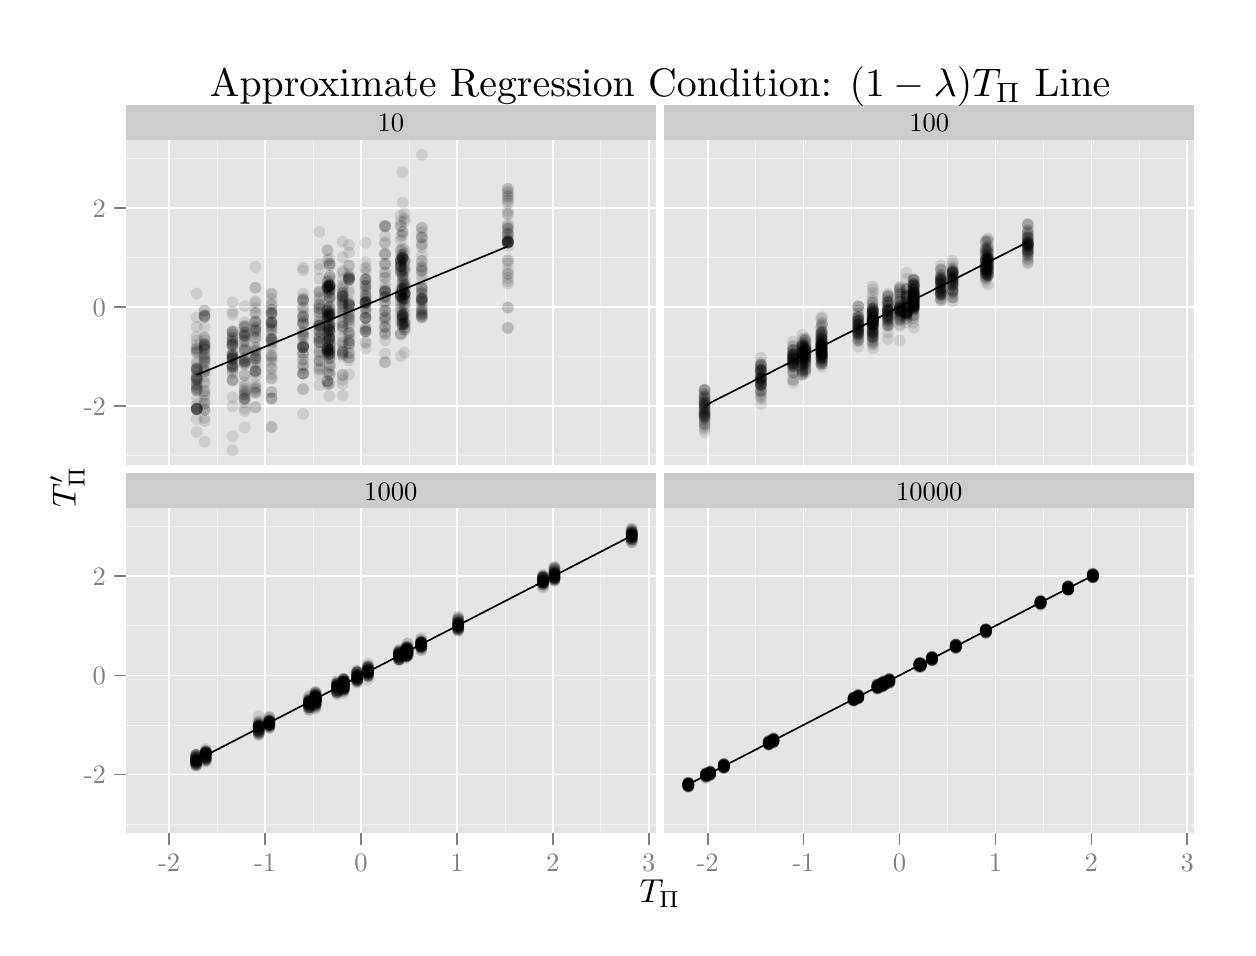
\begin{tikzpicture}[x=1pt,y=1pt]
\definecolor[named]{fillColor}{rgb}{1.00,1.00,1.00}
\path[use as bounding box,fill=fillColor,fill opacity=0.00] (0,0) rectangle (433.62,325.21);
\begin{scope}
\path[clip] (  0.00,  0.00) rectangle (433.62,325.21);
\definecolor[named]{drawColor}{rgb}{1.00,1.00,1.00}
\definecolor[named]{fillColor}{rgb}{1.00,1.00,1.00}

\path[draw=drawColor,line width= 0.6pt,line join=round,line cap=round,fill=fillColor] (  0.00,  0.00) rectangle (433.62,325.21);
\end{scope}
\begin{scope}
\path[clip] ( 35.42,167.14) rectangle (226.99,284.60);
\definecolor[named]{fillColor}{rgb}{0.90,0.90,0.90}

\path[fill=fillColor] ( 35.42,167.14) rectangle (226.99,284.60);
\definecolor[named]{drawColor}{rgb}{0.95,0.95,0.95}

\path[draw=drawColor,line width= 0.3pt,line join=round] ( 35.42,170.55) --
	(226.99,170.55);

\path[draw=drawColor,line width= 0.3pt,line join=round] ( 35.42,206.37) --
	(226.99,206.37);

\path[draw=drawColor,line width= 0.3pt,line join=round] ( 35.42,242.18) --
	(226.99,242.18);

\path[draw=drawColor,line width= 0.3pt,line join=round] ( 35.42,277.99) --
	(226.99,277.99);

\path[draw=drawColor,line width= 0.3pt,line join=round] ( 68.47,167.14) --
	( 68.47,284.60);

\path[draw=drawColor,line width= 0.3pt,line join=round] (103.13,167.14) --
	(103.13,284.60);

\path[draw=drawColor,line width= 0.3pt,line join=round] (137.79,167.14) --
	(137.79,284.60);

\path[draw=drawColor,line width= 0.3pt,line join=round] (172.45,167.14) --
	(172.45,284.60);

\path[draw=drawColor,line width= 0.3pt,line join=round] (207.11,167.14) --
	(207.11,284.60);
\definecolor[named]{drawColor}{rgb}{1.00,1.00,1.00}

\path[draw=drawColor,line width= 0.6pt,line join=round] ( 35.42,188.46) --
	(226.99,188.46);

\path[draw=drawColor,line width= 0.6pt,line join=round] ( 35.42,224.27) --
	(226.99,224.27);

\path[draw=drawColor,line width= 0.6pt,line join=round] ( 35.42,260.09) --
	(226.99,260.09);

\path[draw=drawColor,line width= 0.6pt,line join=round] ( 51.14,167.14) --
	( 51.14,284.60);

\path[draw=drawColor,line width= 0.6pt,line join=round] ( 85.80,167.14) --
	( 85.80,284.60);

\path[draw=drawColor,line width= 0.6pt,line join=round] (120.46,167.14) --
	(120.46,284.60);

\path[draw=drawColor,line width= 0.6pt,line join=round] (155.12,167.14) --
	(155.12,284.60);

\path[draw=drawColor,line width= 0.6pt,line join=round] (189.78,167.14) --
	(189.78,284.60);

\path[draw=drawColor,line width= 0.6pt,line join=round] (224.45,167.14) --
	(224.45,284.60);
\definecolor[named]{fillColor}{rgb}{0.00,0.00,0.00}

\path[fill=fillColor,fill opacity=0.10] (134.84,236.84) circle (  2.13);

\path[fill=fillColor,fill opacity=0.10] (134.84,238.62) circle (  2.13);

\path[fill=fillColor,fill opacity=0.10] (134.84,239.00) circle (  2.13);

\path[fill=fillColor,fill opacity=0.10] (134.84,225.83) circle (  2.13);

\path[fill=fillColor,fill opacity=0.10] (134.84,214.19) circle (  2.13);

\path[fill=fillColor,fill opacity=0.10] (134.84,228.69) circle (  2.13);

\path[fill=fillColor,fill opacity=0.10] (134.84,240.72) circle (  2.13);

\path[fill=fillColor,fill opacity=0.10] (134.84,241.21) circle (  2.13);

\path[fill=fillColor,fill opacity=0.10] (134.84,241.67) circle (  2.13);

\path[fill=fillColor,fill opacity=0.10] (134.84,249.91) circle (  2.13);

\path[fill=fillColor,fill opacity=0.10] (134.84,230.90) circle (  2.13);

\path[fill=fillColor,fill opacity=0.10] (134.84,218.25) circle (  2.13);

\path[fill=fillColor,fill opacity=0.10] (134.84,240.72) circle (  2.13);

\path[fill=fillColor,fill opacity=0.10] (134.84,255.29) circle (  2.13);

\path[fill=fillColor,fill opacity=0.10] (134.84,239.00) circle (  2.13);

\path[fill=fillColor,fill opacity=0.10] (134.84,228.58) circle (  2.13);

\path[fill=fillColor,fill opacity=0.10] (134.84,229.55) circle (  2.13);

\path[fill=fillColor,fill opacity=0.10] (134.84,228.23) circle (  2.13);

\path[fill=fillColor,fill opacity=0.10] (134.84,227.88) circle (  2.13);

\path[fill=fillColor,fill opacity=0.10] (134.84,237.52) circle (  2.13);

\path[fill=fillColor,fill opacity=0.10] (134.84,228.26) circle (  2.13);

\path[fill=fillColor,fill opacity=0.10] (134.84,243.00) circle (  2.13);

\path[fill=fillColor,fill opacity=0.10] (134.84,229.12) circle (  2.13);

\path[fill=fillColor,fill opacity=0.10] (134.84,244.73) circle (  2.13);

\path[fill=fillColor,fill opacity=0.10] (134.84,227.88) circle (  2.13);

\path[fill=fillColor,fill opacity=0.10] (134.84,239.77) circle (  2.13);

\path[fill=fillColor,fill opacity=0.10] (134.84,241.28) circle (  2.13);

\path[fill=fillColor,fill opacity=0.10] (134.84,253.54) circle (  2.13);

\path[fill=fillColor,fill opacity=0.10] (134.84,228.58) circle (  2.13);

\path[fill=fillColor,fill opacity=0.10] (134.84,223.51) circle (  2.13);

\path[fill=fillColor,fill opacity=0.10] (134.84,236.84) circle (  2.13);

\path[fill=fillColor,fill opacity=0.10] (134.84,253.54) circle (  2.13);

\path[fill=fillColor,fill opacity=0.10] (134.84,248.35) circle (  2.13);

\path[fill=fillColor,fill opacity=0.10] (134.84,244.73) circle (  2.13);

\path[fill=fillColor,fill opacity=0.10] (134.84,206.57) circle (  2.13);

\path[fill=fillColor,fill opacity=0.10] (134.84,241.28) circle (  2.13);

\path[fill=fillColor,fill opacity=0.10] (134.84,239.00) circle (  2.13);

\path[fill=fillColor,fill opacity=0.10] (134.84,228.69) circle (  2.13);

\path[fill=fillColor,fill opacity=0.10] (134.84,257.33) circle (  2.13);

\path[fill=fillColor,fill opacity=0.10] (134.84,224.86) circle (  2.13);

\path[fill=fillColor,fill opacity=0.10] (134.84,214.66) circle (  2.13);

\path[fill=fillColor,fill opacity=0.10] (134.84,239.00) circle (  2.13);

\path[fill=fillColor,fill opacity=0.10] (134.84,219.48) circle (  2.13);

\path[fill=fillColor,fill opacity=0.10] (134.84,237.52) circle (  2.13);

\path[fill=fillColor,fill opacity=0.10] (134.84,226.56) circle (  2.13);

\path[fill=fillColor,fill opacity=0.10] (134.84,222.50) circle (  2.13);

\path[fill=fillColor,fill opacity=0.10] (134.84,214.66) circle (  2.13);

\path[fill=fillColor,fill opacity=0.10] (134.84,240.51) circle (  2.13);

\path[fill=fillColor,fill opacity=0.10] (134.84,221.29) circle (  2.13);

\path[fill=fillColor,fill opacity=0.10] (134.84,230.28) circle (  2.13);

\path[fill=fillColor,fill opacity=0.10] (173.52,248.39) circle (  2.13);

\path[fill=fillColor,fill opacity=0.10] (173.52,247.68) circle (  2.13);

\path[fill=fillColor,fill opacity=0.10] (173.52,267.01) circle (  2.13);

\path[fill=fillColor,fill opacity=0.10] (173.52,236.24) circle (  2.13);

\path[fill=fillColor,fill opacity=0.10] (173.52,252.52) circle (  2.13);

\path[fill=fillColor,fill opacity=0.10] (173.52,247.68) circle (  2.13);

\path[fill=fillColor,fill opacity=0.10] (173.52,223.98) circle (  2.13);

\path[fill=fillColor,fill opacity=0.10] (173.52,237.61) circle (  2.13);

\path[fill=fillColor,fill opacity=0.10] (173.52,247.97) circle (  2.13);

\path[fill=fillColor,fill opacity=0.10] (173.52,261.66) circle (  2.13);

\path[fill=fillColor,fill opacity=0.10] (173.52,216.70) circle (  2.13);

\path[fill=fillColor,fill opacity=0.10] (173.52,216.70) circle (  2.13);

\path[fill=fillColor,fill opacity=0.10] (173.52,250.83) circle (  2.13);

\path[fill=fillColor,fill opacity=0.10] (173.52,246.40) circle (  2.13);

\path[fill=fillColor,fill opacity=0.10] (173.52,232.71) circle (  2.13);

\path[fill=fillColor,fill opacity=0.10] (173.52,247.68) circle (  2.13);

\path[fill=fillColor,fill opacity=0.10] (173.52,247.64) circle (  2.13);

\path[fill=fillColor,fill opacity=0.10] (173.52,247.64) circle (  2.13);

\path[fill=fillColor,fill opacity=0.10] (173.52,258.98) circle (  2.13);

\path[fill=fillColor,fill opacity=0.10] (173.52,265.39) circle (  2.13);

\path[fill=fillColor,fill opacity=0.10] (173.52,258.09) circle (  2.13);

\path[fill=fillColor,fill opacity=0.10] (173.52,247.77) circle (  2.13);

\path[fill=fillColor,fill opacity=0.10] (173.52,252.94) circle (  2.13);

\path[fill=fillColor,fill opacity=0.10] (173.52,248.66) circle (  2.13);

\path[fill=fillColor,fill opacity=0.10] (173.52,257.65) circle (  2.13);

\path[fill=fillColor,fill opacity=0.10] (173.52,267.01) circle (  2.13);

\path[fill=fillColor,fill opacity=0.10] (173.52,252.52) circle (  2.13);

\path[fill=fillColor,fill opacity=0.10] (173.52,264.15) circle (  2.13);

\path[fill=fillColor,fill opacity=0.10] (173.52,247.68) circle (  2.13);

\path[fill=fillColor,fill opacity=0.10] (173.52,262.67) circle (  2.13);

\path[fill=fillColor,fill opacity=0.10] (173.52,247.64) circle (  2.13);

\path[fill=fillColor,fill opacity=0.10] (173.52,240.99) circle (  2.13);

\path[fill=fillColor,fill opacity=0.10] (173.52,251.13) circle (  2.13);

\path[fill=fillColor,fill opacity=0.10] (173.52,263.07) circle (  2.13);

\path[fill=fillColor,fill opacity=0.10] (173.52,236.24) circle (  2.13);

\path[fill=fillColor,fill opacity=0.10] (173.52,233.62) circle (  2.13);

\path[fill=fillColor,fill opacity=0.10] (173.52,248.39) circle (  2.13);

\path[fill=fillColor,fill opacity=0.10] (173.52,224.10) circle (  2.13);

\path[fill=fillColor,fill opacity=0.10] (173.52,247.37) circle (  2.13);

\path[fill=fillColor,fill opacity=0.10] (173.52,239.98) circle (  2.13);

\path[fill=fillColor,fill opacity=0.10] (173.52,254.29) circle (  2.13);

\path[fill=fillColor,fill opacity=0.10] (173.52,249.31) circle (  2.13);

\path[fill=fillColor,fill opacity=0.10] (173.52,266.00) circle (  2.13);

\path[fill=fillColor,fill opacity=0.10] (173.52,250.53) circle (  2.13);

\path[fill=fillColor,fill opacity=0.10] (173.52,234.75) circle (  2.13);

\path[fill=fillColor,fill opacity=0.10] (173.52,253.62) circle (  2.13);

\path[fill=fillColor,fill opacity=0.10] (173.52,264.40) circle (  2.13);

\path[fill=fillColor,fill opacity=0.10] (173.52,247.41) circle (  2.13);

\path[fill=fillColor,fill opacity=0.10] (173.52,241.33) circle (  2.13);

\path[fill=fillColor,fill opacity=0.10] (173.52,250.53) circle (  2.13);

\path[fill=fillColor,fill opacity=0.10] ( 61.09,179.12) circle (  2.13);

\path[fill=fillColor,fill opacity=0.10] ( 61.09,220.47) circle (  2.13);

\path[fill=fillColor,fill opacity=0.10] ( 61.09,210.65) circle (  2.13);

\path[fill=fillColor,fill opacity=0.10] ( 61.09,194.47) circle (  2.13);

\path[fill=fillColor,fill opacity=0.10] ( 61.09,200.80) circle (  2.13);

\path[fill=fillColor,fill opacity=0.10] ( 61.09,196.32) circle (  2.13);

\path[fill=fillColor,fill opacity=0.10] ( 61.09,207.63) circle (  2.13);

\path[fill=fillColor,fill opacity=0.10] ( 61.09,198.22) circle (  2.13);

\path[fill=fillColor,fill opacity=0.10] ( 61.09,188.87) circle (  2.13);

\path[fill=fillColor,fill opacity=0.10] ( 61.09,187.34) circle (  2.13);

\path[fill=fillColor,fill opacity=0.10] ( 61.09,201.71) circle (  2.13);

\path[fill=fillColor,fill opacity=0.10] ( 61.09,194.13) circle (  2.13);

\path[fill=fillColor,fill opacity=0.10] ( 61.09,203.91) circle (  2.13);

\path[fill=fillColor,fill opacity=0.10] ( 61.09,195.35) circle (  2.13);

\path[fill=fillColor,fill opacity=0.10] ( 61.09,209.33) circle (  2.13);

\path[fill=fillColor,fill opacity=0.10] ( 61.09,198.22) circle (  2.13);

\path[fill=fillColor,fill opacity=0.10] ( 61.09,198.96) circle (  2.13);

\path[fill=fillColor,fill opacity=0.10] ( 61.09,187.38) circle (  2.13);

\path[fill=fillColor,fill opacity=0.10] ( 61.09,208.13) circle (  2.13);

\path[fill=fillColor,fill opacity=0.10] ( 61.09,202.37) circle (  2.13);

\path[fill=fillColor,fill opacity=0.10] ( 61.09,191.04) circle (  2.13);

\path[fill=fillColor,fill opacity=0.10] ( 61.09,187.46) circle (  2.13);

\path[fill=fillColor,fill opacity=0.10] ( 61.09,187.34) circle (  2.13);

\path[fill=fillColor,fill opacity=0.10] ( 61.09,196.32) circle (  2.13);

\path[fill=fillColor,fill opacity=0.10] ( 61.09,194.13) circle (  2.13);

\path[fill=fillColor,fill opacity=0.10] ( 61.09,208.77) circle (  2.13);

\path[fill=fillColor,fill opacity=0.10] ( 61.09,213.64) circle (  2.13);

\path[fill=fillColor,fill opacity=0.10] ( 61.09,195.35) circle (  2.13);

\path[fill=fillColor,fill opacity=0.10] ( 61.09,197.54) circle (  2.13);

\path[fill=fillColor,fill opacity=0.10] ( 61.09,187.38) circle (  2.13);

\path[fill=fillColor,fill opacity=0.10] ( 61.09,187.67) circle (  2.13);

\path[fill=fillColor,fill opacity=0.10] ( 61.09,201.71) circle (  2.13);

\path[fill=fillColor,fill opacity=0.10] ( 61.09,194.71) circle (  2.13);

\path[fill=fillColor,fill opacity=0.10] ( 61.09,202.00) circle (  2.13);

\path[fill=fillColor,fill opacity=0.10] ( 61.09,198.05) circle (  2.13);

\path[fill=fillColor,fill opacity=0.10] ( 61.09,183.72) circle (  2.13);

\path[fill=fillColor,fill opacity=0.10] ( 61.09,217.12) circle (  2.13);

\path[fill=fillColor,fill opacity=0.10] ( 61.09,187.38) circle (  2.13);

\path[fill=fillColor,fill opacity=0.10] ( 61.09,198.22) circle (  2.13);

\path[fill=fillColor,fill opacity=0.10] ( 61.09,198.96) circle (  2.13);

\path[fill=fillColor,fill opacity=0.10] ( 61.09,212.09) circle (  2.13);

\path[fill=fillColor,fill opacity=0.10] ( 61.09,187.46) circle (  2.13);

\path[fill=fillColor,fill opacity=0.10] ( 61.09,208.13) circle (  2.13);

\path[fill=fillColor,fill opacity=0.10] ( 61.09,204.42) circle (  2.13);

\path[fill=fillColor,fill opacity=0.10] ( 61.09,201.71) circle (  2.13);

\path[fill=fillColor,fill opacity=0.10] ( 61.09,209.33) circle (  2.13);

\path[fill=fillColor,fill opacity=0.10] ( 61.09,202.00) circle (  2.13);

\path[fill=fillColor,fill opacity=0.10] ( 61.09,199.36) circle (  2.13);

\path[fill=fillColor,fill opacity=0.10] ( 61.09,229.16) circle (  2.13);

\path[fill=fillColor,fill opacity=0.10] ( 61.09,187.46) circle (  2.13);

\path[fill=fillColor,fill opacity=0.10] ( 78.40,203.68) circle (  2.13);

\path[fill=fillColor,fill opacity=0.10] ( 78.40,208.61) circle (  2.13);

\path[fill=fillColor,fill opacity=0.10] ( 78.40,195.77) circle (  2.13);

\path[fill=fillColor,fill opacity=0.10] ( 78.40,213.90) circle (  2.13);

\path[fill=fillColor,fill opacity=0.10] ( 78.40,191.03) circle (  2.13);

\path[fill=fillColor,fill opacity=0.10] ( 78.40,211.45) circle (  2.13);

\path[fill=fillColor,fill opacity=0.10] ( 78.40,208.61) circle (  2.13);

\path[fill=fillColor,fill opacity=0.10] ( 78.40,208.61) circle (  2.13);

\path[fill=fillColor,fill opacity=0.10] ( 78.40,192.83) circle (  2.13);

\path[fill=fillColor,fill opacity=0.10] ( 78.40,213.66) circle (  2.13);

\path[fill=fillColor,fill opacity=0.10] ( 78.40,205.87) circle (  2.13);

\path[fill=fillColor,fill opacity=0.10] ( 78.40,180.71) circle (  2.13);

\path[fill=fillColor,fill opacity=0.10] ( 78.40,193.85) circle (  2.13);

\path[fill=fillColor,fill opacity=0.10] ( 78.40,224.58) circle (  2.13);

\path[fill=fillColor,fill opacity=0.10] ( 78.40,204.12) circle (  2.13);

\path[fill=fillColor,fill opacity=0.10] ( 78.40,199.52) circle (  2.13);

\path[fill=fillColor,fill opacity=0.10] ( 78.40,193.85) circle (  2.13);

\path[fill=fillColor,fill opacity=0.10] ( 78.40,217.32) circle (  2.13);

\path[fill=fillColor,fill opacity=0.10] ( 78.40,204.65) circle (  2.13);

\path[fill=fillColor,fill opacity=0.10] ( 78.40,192.83) circle (  2.13);

\path[fill=fillColor,fill opacity=0.10] ( 78.40,209.11) circle (  2.13);

\path[fill=fillColor,fill opacity=0.10] ( 78.40,217.60) circle (  2.13);

\path[fill=fillColor,fill opacity=0.10] ( 78.40,215.08) circle (  2.13);

\path[fill=fillColor,fill opacity=0.10] ( 78.40,189.81) circle (  2.13);

\path[fill=fillColor,fill opacity=0.10] ( 78.40,218.75) circle (  2.13);

\path[fill=fillColor,fill opacity=0.10] ( 78.40,214.09) circle (  2.13);

\path[fill=fillColor,fill opacity=0.10] ( 78.40,216.95) circle (  2.13);

\path[fill=fillColor,fill opacity=0.10] ( 78.40,194.66) circle (  2.13);

\path[fill=fillColor,fill opacity=0.10] ( 78.40,210.04) circle (  2.13);

\path[fill=fillColor,fill opacity=0.10] ( 78.40,199.82) circle (  2.13);

\path[fill=fillColor,fill opacity=0.10] ( 78.40,204.65) circle (  2.13);

\path[fill=fillColor,fill opacity=0.10] ( 78.40,205.87) circle (  2.13);

\path[fill=fillColor,fill opacity=0.10] ( 78.40,204.65) circle (  2.13);

\path[fill=fillColor,fill opacity=0.10] ( 78.40,216.95) circle (  2.13);

\path[fill=fillColor,fill opacity=0.10] ( 78.40,187.62) circle (  2.13);

\path[fill=fillColor,fill opacity=0.10] ( 78.40,214.09) circle (  2.13);

\path[fill=fillColor,fill opacity=0.10] ( 78.40,212.00) circle (  2.13);

\path[fill=fillColor,fill opacity=0.10] ( 78.40,204.92) circle (  2.13);

\path[fill=fillColor,fill opacity=0.10] ( 78.40,186.61) circle (  2.13);

\path[fill=fillColor,fill opacity=0.10] ( 78.40,192.18) circle (  2.13);

\path[fill=fillColor,fill opacity=0.10] ( 78.40,203.50) circle (  2.13);

\path[fill=fillColor,fill opacity=0.10] ( 78.40,191.03) circle (  2.13);

\path[fill=fillColor,fill opacity=0.10] ( 78.40,214.78) circle (  2.13);

\path[fill=fillColor,fill opacity=0.10] ( 78.40,212.44) circle (  2.13);

\path[fill=fillColor,fill opacity=0.10] ( 78.40,191.58) circle (  2.13);

\path[fill=fillColor,fill opacity=0.10] ( 78.40,215.08) circle (  2.13);

\path[fill=fillColor,fill opacity=0.10] ( 78.40,213.84) circle (  2.13);

\path[fill=fillColor,fill opacity=0.10] ( 78.40,191.18) circle (  2.13);

\path[fill=fillColor,fill opacity=0.10] ( 78.40,197.04) circle (  2.13);

\path[fill=fillColor,fill opacity=0.10] ( 78.40,204.12) circle (  2.13);

\path[fill=fillColor,fill opacity=0.10] (135.46,220.39) circle (  2.13);

\path[fill=fillColor,fill opacity=0.10] (135.46,273.01) circle (  2.13);

\path[fill=fillColor,fill opacity=0.10] (135.46,250.28) circle (  2.13);

\path[fill=fillColor,fill opacity=0.10] (135.46,231.16) circle (  2.13);

\path[fill=fillColor,fill opacity=0.10] (135.46,220.22) circle (  2.13);

\path[fill=fillColor,fill opacity=0.10] (135.46,235.80) circle (  2.13);

\path[fill=fillColor,fill opacity=0.10] (135.46,221.60) circle (  2.13);

\path[fill=fillColor,fill opacity=0.10] (135.46,221.36) circle (  2.13);

\path[fill=fillColor,fill opacity=0.10] (135.46,235.55) circle (  2.13);

\path[fill=fillColor,fill opacity=0.10] (135.46,242.01) circle (  2.13);

\path[fill=fillColor,fill opacity=0.10] (135.46,218.00) circle (  2.13);

\path[fill=fillColor,fill opacity=0.10] (135.46,230.92) circle (  2.13);

\path[fill=fillColor,fill opacity=0.10] (135.46,251.48) circle (  2.13);

\path[fill=fillColor,fill opacity=0.10] (135.46,222.53) circle (  2.13);

\path[fill=fillColor,fill opacity=0.10] (135.46,245.47) circle (  2.13);

\path[fill=fillColor,fill opacity=0.10] (135.46,233.08) circle (  2.13);

\path[fill=fillColor,fill opacity=0.10] (135.46,218.19) circle (  2.13);

\path[fill=fillColor,fill opacity=0.10] (135.46,221.43) circle (  2.13);

\path[fill=fillColor,fill opacity=0.10] (135.46,220.22) circle (  2.13);

\path[fill=fillColor,fill opacity=0.10] (135.46,220.94) circle (  2.13);

\path[fill=fillColor,fill opacity=0.10] (135.46,234.44) circle (  2.13);

\path[fill=fillColor,fill opacity=0.10] (135.46,218.00) circle (  2.13);

\path[fill=fillColor,fill opacity=0.10] (135.46,221.19) circle (  2.13);

\path[fill=fillColor,fill opacity=0.10] (135.46,218.00) circle (  2.13);

\path[fill=fillColor,fill opacity=0.10] (135.46,251.48) circle (  2.13);

\path[fill=fillColor,fill opacity=0.10] (135.46,261.98) circle (  2.13);

\path[fill=fillColor,fill opacity=0.10] (135.46,242.01) circle (  2.13);

\path[fill=fillColor,fill opacity=0.10] (135.46,237.65) circle (  2.13);

\path[fill=fillColor,fill opacity=0.10] (135.46,218.72) circle (  2.13);

\path[fill=fillColor,fill opacity=0.10] (135.46,219.42) circle (  2.13);

\path[fill=fillColor,fill opacity=0.10] (135.46,242.01) circle (  2.13);

\path[fill=fillColor,fill opacity=0.10] (135.46,229.99) circle (  2.13);

\path[fill=fillColor,fill opacity=0.10] (135.46,230.68) circle (  2.13);

\path[fill=fillColor,fill opacity=0.10] (135.46,236.85) circle (  2.13);

\path[fill=fillColor,fill opacity=0.10] (135.46,227.56) circle (  2.13);

\path[fill=fillColor,fill opacity=0.10] (135.46,232.49) circle (  2.13);

\path[fill=fillColor,fill opacity=0.10] (135.46,242.06) circle (  2.13);

\path[fill=fillColor,fill opacity=0.10] (135.46,235.25) circle (  2.13);

\path[fill=fillColor,fill opacity=0.10] (135.46,226.98) circle (  2.13);

\path[fill=fillColor,fill opacity=0.10] (135.46,242.01) circle (  2.13);

\path[fill=fillColor,fill opacity=0.10] (135.46,224.91) circle (  2.13);

\path[fill=fillColor,fill opacity=0.10] (135.46,243.11) circle (  2.13);

\path[fill=fillColor,fill opacity=0.10] (135.46,217.39) circle (  2.13);

\path[fill=fillColor,fill opacity=0.10] (135.46,241.55) circle (  2.13);

\path[fill=fillColor,fill opacity=0.10] (135.46,233.08) circle (  2.13);

\path[fill=fillColor,fill opacity=0.10] (135.46,230.68) circle (  2.13);

\path[fill=fillColor,fill opacity=0.10] (135.46,227.56) circle (  2.13);

\path[fill=fillColor,fill opacity=0.10] (135.46,242.92) circle (  2.13);

\path[fill=fillColor,fill opacity=0.10] (135.46,220.94) circle (  2.13);

\path[fill=fillColor,fill opacity=0.10] (135.46,227.15) circle (  2.13);

\path[fill=fillColor,fill opacity=0.10] ( 74.01,213.27) circle (  2.13);

\path[fill=fillColor,fill opacity=0.10] ( 74.01,188.42) circle (  2.13);

\path[fill=fillColor,fill opacity=0.10] ( 74.01,211.72) circle (  2.13);

\path[fill=fillColor,fill opacity=0.10] ( 74.01,207.13) circle (  2.13);

\path[fill=fillColor,fill opacity=0.10] ( 74.01,177.58) circle (  2.13);

\path[fill=fillColor,fill opacity=0.10] ( 74.01,206.47) circle (  2.13);

\path[fill=fillColor,fill opacity=0.10] ( 74.01,222.58) circle (  2.13);

\path[fill=fillColor,fill opacity=0.10] ( 74.01,214.92) circle (  2.13);

\path[fill=fillColor,fill opacity=0.10] ( 74.01,203.78) circle (  2.13);

\path[fill=fillColor,fill opacity=0.10] ( 74.01,207.13) circle (  2.13);

\path[fill=fillColor,fill opacity=0.10] ( 74.01,207.82) circle (  2.13);

\path[fill=fillColor,fill opacity=0.10] ( 74.01,202.70) circle (  2.13);

\path[fill=fillColor,fill opacity=0.10] ( 74.01,203.48) circle (  2.13);

\path[fill=fillColor,fill opacity=0.10] ( 74.01,221.49) circle (  2.13);

\path[fill=fillColor,fill opacity=0.10] ( 74.01,206.00) circle (  2.13);

\path[fill=fillColor,fill opacity=0.10] ( 74.01,205.54) circle (  2.13);

\path[fill=fillColor,fill opacity=0.10] ( 74.01,202.43) circle (  2.13);

\path[fill=fillColor,fill opacity=0.10] ( 74.01,215.28) circle (  2.13);

\path[fill=fillColor,fill opacity=0.10] ( 74.01,210.11) circle (  2.13);

\path[fill=fillColor,fill opacity=0.10] ( 74.01,191.68) circle (  2.13);

\path[fill=fillColor,fill opacity=0.10] ( 74.01,210.70) circle (  2.13);

\path[fill=fillColor,fill opacity=0.10] ( 74.01,202.70) circle (  2.13);

\path[fill=fillColor,fill opacity=0.10] ( 74.01,212.03) circle (  2.13);

\path[fill=fillColor,fill opacity=0.10] ( 74.01,206.38) circle (  2.13);

\path[fill=fillColor,fill opacity=0.10] ( 74.01,197.69) circle (  2.13);

\path[fill=fillColor,fill opacity=0.10] ( 74.01,215.57) circle (  2.13);

\path[fill=fillColor,fill opacity=0.10] ( 74.01,213.27) circle (  2.13);

\path[fill=fillColor,fill opacity=0.10] ( 74.01,200.28) circle (  2.13);

\path[fill=fillColor,fill opacity=0.10] ( 74.01,197.93) circle (  2.13);

\path[fill=fillColor,fill opacity=0.10] ( 74.01,211.78) circle (  2.13);

\path[fill=fillColor,fill opacity=0.10] ( 74.01,214.16) circle (  2.13);

\path[fill=fillColor,fill opacity=0.10] ( 74.01,210.36) circle (  2.13);

\path[fill=fillColor,fill opacity=0.10] ( 74.01,202.99) circle (  2.13);

\path[fill=fillColor,fill opacity=0.10] ( 74.01,206.00) circle (  2.13);

\path[fill=fillColor,fill opacity=0.10] ( 74.01,215.39) circle (  2.13);

\path[fill=fillColor,fill opacity=0.10] ( 74.01,202.99) circle (  2.13);

\path[fill=fillColor,fill opacity=0.10] ( 74.01,201.89) circle (  2.13);

\path[fill=fillColor,fill opacity=0.10] ( 74.01,206.78) circle (  2.13);

\path[fill=fillColor,fill opacity=0.10] ( 74.01,226.03) circle (  2.13);

\path[fill=fillColor,fill opacity=0.10] ( 74.01,206.78) circle (  2.13);

\path[fill=fillColor,fill opacity=0.10] ( 74.01,210.40) circle (  2.13);

\path[fill=fillColor,fill opacity=0.10] ( 74.01,197.93) circle (  2.13);

\path[fill=fillColor,fill opacity=0.10] ( 74.01,201.10) circle (  2.13);

\path[fill=fillColor,fill opacity=0.10] ( 74.01,212.60) circle (  2.13);

\path[fill=fillColor,fill opacity=0.10] ( 74.01,205.54) circle (  2.13);

\path[fill=fillColor,fill opacity=0.10] ( 74.01,172.48) circle (  2.13);

\path[fill=fillColor,fill opacity=0.10] ( 74.01,210.89) circle (  2.13);

\path[fill=fillColor,fill opacity=0.10] ( 74.01,205.24) circle (  2.13);

\path[fill=fillColor,fill opacity=0.10] ( 74.01,205.24) circle (  2.13);

\path[fill=fillColor,fill opacity=0.10] ( 74.01,210.89) circle (  2.13);

\path[fill=fillColor,fill opacity=0.10] (142.43,229.73) circle (  2.13);

\path[fill=fillColor,fill opacity=0.10] (142.43,227.39) circle (  2.13);

\path[fill=fillColor,fill opacity=0.10] (142.43,231.74) circle (  2.13);

\path[fill=fillColor,fill opacity=0.10] (142.43,238.77) circle (  2.13);

\path[fill=fillColor,fill opacity=0.10] (142.43,220.47) circle (  2.13);

\path[fill=fillColor,fill opacity=0.10] (142.43,222.33) circle (  2.13);

\path[fill=fillColor,fill opacity=0.10] (142.43,237.28) circle (  2.13);

\path[fill=fillColor,fill opacity=0.10] (142.43,229.16) circle (  2.13);

\path[fill=fillColor,fill opacity=0.10] (142.43,252.90) circle (  2.13);

\path[fill=fillColor,fill opacity=0.10] (142.43,230.99) circle (  2.13);

\path[fill=fillColor,fill opacity=0.10] (142.43,221.90) circle (  2.13);

\path[fill=fillColor,fill opacity=0.10] (142.43,227.02) circle (  2.13);

\path[fill=fillColor,fill opacity=0.10] (142.43,252.90) circle (  2.13);

\path[fill=fillColor,fill opacity=0.10] (142.43,234.18) circle (  2.13);

\path[fill=fillColor,fill opacity=0.10] (142.43,251.32) circle (  2.13);

\path[fill=fillColor,fill opacity=0.10] (142.43,223.92) circle (  2.13);

\path[fill=fillColor,fill opacity=0.10] (142.43,242.94) circle (  2.13);

\path[fill=fillColor,fill opacity=0.10] (142.43,247.03) circle (  2.13);

\path[fill=fillColor,fill opacity=0.10] (142.43,227.02) circle (  2.13);

\path[fill=fillColor,fill opacity=0.10] (142.43,247.03) circle (  2.13);

\path[fill=fillColor,fill opacity=0.10] (142.43,227.39) circle (  2.13);

\path[fill=fillColor,fill opacity=0.10] (142.43,226.30) circle (  2.13);

\path[fill=fillColor,fill opacity=0.10] (142.43,229.16) circle (  2.13);

\path[fill=fillColor,fill opacity=0.10] (142.43,249.32) circle (  2.13);

\path[fill=fillColor,fill opacity=0.10] (142.43,230.83) circle (  2.13);

\path[fill=fillColor,fill opacity=0.10] (142.43,249.49) circle (  2.13);

\path[fill=fillColor,fill opacity=0.10] (142.43,227.16) circle (  2.13);

\path[fill=fillColor,fill opacity=0.10] (142.43,226.27) circle (  2.13);

\path[fill=fillColor,fill opacity=0.10] (142.43,279.26) circle (  2.13);

\path[fill=fillColor,fill opacity=0.10] (142.43,221.44) circle (  2.13);

\path[fill=fillColor,fill opacity=0.10] (142.43,238.03) circle (  2.13);

\path[fill=fillColor,fill opacity=0.10] (142.43,240.89) circle (  2.13);

\path[fill=fillColor,fill opacity=0.10] (142.43,223.32) circle (  2.13);

\path[fill=fillColor,fill opacity=0.10] (142.43,238.77) circle (  2.13);

\path[fill=fillColor,fill opacity=0.10] (142.43,224.89) circle (  2.13);

\path[fill=fillColor,fill opacity=0.10] (142.43,225.98) circle (  2.13);

\path[fill=fillColor,fill opacity=0.10] (142.43,235.81) circle (  2.13);

\path[fill=fillColor,fill opacity=0.10] (142.43,221.55) circle (  2.13);

\path[fill=fillColor,fill opacity=0.10] (142.43,222.64) circle (  2.13);

\path[fill=fillColor,fill opacity=0.10] (142.43,223.32) circle (  2.13);

\path[fill=fillColor,fill opacity=0.10] (142.43,237.28) circle (  2.13);

\path[fill=fillColor,fill opacity=0.10] (142.43,240.89) circle (  2.13);

\path[fill=fillColor,fill opacity=0.10] (142.43,220.93) circle (  2.13);

\path[fill=fillColor,fill opacity=0.10] (142.43,227.74) circle (  2.13);

\path[fill=fillColor,fill opacity=0.10] (142.43,220.93) circle (  2.13);

\path[fill=fillColor,fill opacity=0.10] (142.43,227.02) circle (  2.13);

\path[fill=fillColor,fill opacity=0.10] (142.43,249.49) circle (  2.13);

\path[fill=fillColor,fill opacity=0.10] (142.43,230.99) circle (  2.13);

\path[fill=fillColor,fill opacity=0.10] (142.43,220.47) circle (  2.13);

\path[fill=fillColor,fill opacity=0.10] (142.43,245.94) circle (  2.13);

\path[fill=fillColor,fill opacity=0.10] ( 63.91,206.05) circle (  2.13);

\path[fill=fillColor,fill opacity=0.10] ( 63.91,187.05) circle (  2.13);

\path[fill=fillColor,fill opacity=0.10] ( 63.91,213.24) circle (  2.13);

\path[fill=fillColor,fill opacity=0.10] ( 63.91,175.61) circle (  2.13);

\path[fill=fillColor,fill opacity=0.10] ( 63.91,187.05) circle (  2.13);

\path[fill=fillColor,fill opacity=0.10] ( 63.91,212.24) circle (  2.13);

\path[fill=fillColor,fill opacity=0.10] ( 63.91,205.10) circle (  2.13);

\path[fill=fillColor,fill opacity=0.10] ( 63.91,190.35) circle (  2.13);

\path[fill=fillColor,fill opacity=0.10] ( 63.91,200.99) circle (  2.13);

\path[fill=fillColor,fill opacity=0.10] ( 63.91,196.99) circle (  2.13);

\path[fill=fillColor,fill opacity=0.10] ( 63.91,201.73) circle (  2.13);

\path[fill=fillColor,fill opacity=0.10] ( 63.91,207.08) circle (  2.13);

\path[fill=fillColor,fill opacity=0.10] ( 63.91,221.18) circle (  2.13);

\path[fill=fillColor,fill opacity=0.10] ( 63.91,189.25) circle (  2.13);

\path[fill=fillColor,fill opacity=0.10] ( 63.91,210.12) circle (  2.13);

\path[fill=fillColor,fill opacity=0.10] ( 63.91,204.48) circle (  2.13);

\path[fill=fillColor,fill opacity=0.10] ( 63.91,221.18) circle (  2.13);

\path[fill=fillColor,fill opacity=0.10] ( 63.91,193.81) circle (  2.13);

\path[fill=fillColor,fill opacity=0.10] ( 63.91,208.88) circle (  2.13);

\path[fill=fillColor,fill opacity=0.10] ( 63.91,210.38) circle (  2.13);

\path[fill=fillColor,fill opacity=0.10] ( 63.91,205.10) circle (  2.13);

\path[fill=fillColor,fill opacity=0.10] ( 63.91,217.08) circle (  2.13);

\path[fill=fillColor,fill opacity=0.10] ( 63.91,204.48) circle (  2.13);

\path[fill=fillColor,fill opacity=0.10] ( 63.91,220.75) circle (  2.13);

\path[fill=fillColor,fill opacity=0.10] ( 63.91,194.01) circle (  2.13);

\path[fill=fillColor,fill opacity=0.10] ( 63.91,189.41) circle (  2.13);

\path[fill=fillColor,fill opacity=0.10] ( 63.91,192.70) circle (  2.13);

\path[fill=fillColor,fill opacity=0.10] ( 63.91,222.96) circle (  2.13);

\path[fill=fillColor,fill opacity=0.10] ( 63.91,221.18) circle (  2.13);

\path[fill=fillColor,fill opacity=0.10] ( 63.91,209.28) circle (  2.13);

\path[fill=fillColor,fill opacity=0.10] ( 63.91,210.95) circle (  2.13);

\path[fill=fillColor,fill opacity=0.10] ( 63.91,213.24) circle (  2.13);

\path[fill=fillColor,fill opacity=0.10] ( 63.91,202.91) circle (  2.13);

\path[fill=fillColor,fill opacity=0.10] ( 63.91,200.99) circle (  2.13);

\path[fill=fillColor,fill opacity=0.10] ( 63.91,210.12) circle (  2.13);

\path[fill=fillColor,fill opacity=0.10] ( 63.91,208.88) circle (  2.13);

\path[fill=fillColor,fill opacity=0.10] ( 63.91,187.85) circle (  2.13);

\path[fill=fillColor,fill opacity=0.10] ( 63.91,200.99) circle (  2.13);

\path[fill=fillColor,fill opacity=0.10] ( 63.91,192.09) circle (  2.13);

\path[fill=fillColor,fill opacity=0.10] ( 63.91,210.76) circle (  2.13);

\path[fill=fillColor,fill opacity=0.10] ( 63.91,184.10) circle (  2.13);

\path[fill=fillColor,fill opacity=0.10] ( 63.91,183.06) circle (  2.13);

\path[fill=fillColor,fill opacity=0.10] ( 63.91,209.44) circle (  2.13);

\path[fill=fillColor,fill opacity=0.10] ( 63.91,199.15) circle (  2.13);

\path[fill=fillColor,fill opacity=0.10] ( 63.91,222.96) circle (  2.13);

\path[fill=fillColor,fill opacity=0.10] ( 63.91,210.95) circle (  2.13);

\path[fill=fillColor,fill opacity=0.10] ( 63.91,220.71) circle (  2.13);

\path[fill=fillColor,fill opacity=0.10] ( 63.91,196.67) circle (  2.13);

\path[fill=fillColor,fill opacity=0.10] ( 63.91,207.08) circle (  2.13);

\path[fill=fillColor,fill opacity=0.10] ( 63.91,206.03) circle (  2.13);

\path[fill=fillColor,fill opacity=0.10] (122.09,216.41) circle (  2.13);

\path[fill=fillColor,fill opacity=0.10] (122.09,240.50) circle (  2.13);

\path[fill=fillColor,fill opacity=0.10] (122.09,220.41) circle (  2.13);

\path[fill=fillColor,fill opacity=0.10] (122.09,237.98) circle (  2.13);

\path[fill=fillColor,fill opacity=0.10] (122.09,215.35) circle (  2.13);

\path[fill=fillColor,fill opacity=0.10] (122.09,223.70) circle (  2.13);

\path[fill=fillColor,fill opacity=0.10] (122.09,228.13) circle (  2.13);

\path[fill=fillColor,fill opacity=0.10] (122.09,230.71) circle (  2.13);

\path[fill=fillColor,fill opacity=0.10] (122.09,222.11) circle (  2.13);

\path[fill=fillColor,fill opacity=0.10] (122.09,225.91) circle (  2.13);

\path[fill=fillColor,fill opacity=0.10] (122.09,209.27) circle (  2.13);

\path[fill=fillColor,fill opacity=0.10] (122.09,224.42) circle (  2.13);

\path[fill=fillColor,fill opacity=0.10] (122.09,223.70) circle (  2.13);

\path[fill=fillColor,fill opacity=0.10] (122.09,231.96) circle (  2.13);

\path[fill=fillColor,fill opacity=0.10] (122.09,226.00) circle (  2.13);

\path[fill=fillColor,fill opacity=0.10] (122.09,226.08) circle (  2.13);

\path[fill=fillColor,fill opacity=0.10] (122.09,234.34) circle (  2.13);

\path[fill=fillColor,fill opacity=0.10] (122.09,226.00) circle (  2.13);

\path[fill=fillColor,fill opacity=0.10] (122.09,227.01) circle (  2.13);

\path[fill=fillColor,fill opacity=0.10] (122.09,228.53) circle (  2.13);

\path[fill=fillColor,fill opacity=0.10] (122.09,234.16) circle (  2.13);

\path[fill=fillColor,fill opacity=0.10] (122.09,215.53) circle (  2.13);

\path[fill=fillColor,fill opacity=0.10] (122.09,231.96) circle (  2.13);

\path[fill=fillColor,fill opacity=0.10] (122.09,225.91) circle (  2.13);

\path[fill=fillColor,fill opacity=0.10] (122.09,227.12) circle (  2.13);

\path[fill=fillColor,fill opacity=0.10] (122.09,230.60) circle (  2.13);

\path[fill=fillColor,fill opacity=0.10] (122.09,234.37) circle (  2.13);

\path[fill=fillColor,fill opacity=0.10] (122.09,220.41) circle (  2.13);

\path[fill=fillColor,fill opacity=0.10] (122.09,211.15) circle (  2.13);

\path[fill=fillColor,fill opacity=0.10] (122.09,217.33) circle (  2.13);

\path[fill=fillColor,fill opacity=0.10] (122.09,216.30) circle (  2.13);

\path[fill=fillColor,fill opacity=0.10] (122.09,231.96) circle (  2.13);

\path[fill=fillColor,fill opacity=0.10] (122.09,232.96) circle (  2.13);

\path[fill=fillColor,fill opacity=0.10] (122.09,238.57) circle (  2.13);

\path[fill=fillColor,fill opacity=0.10] (122.09,234.34) circle (  2.13);

\path[fill=fillColor,fill opacity=0.10] (122.09,225.58) circle (  2.13);

\path[fill=fillColor,fill opacity=0.10] (122.09,220.34) circle (  2.13);

\path[fill=fillColor,fill opacity=0.10] (122.09,226.08) circle (  2.13);

\path[fill=fillColor,fill opacity=0.10] (122.09,215.45) circle (  2.13);

\path[fill=fillColor,fill opacity=0.10] (122.09,220.34) circle (  2.13);

\path[fill=fillColor,fill opacity=0.10] (122.09,220.34) circle (  2.13);

\path[fill=fillColor,fill opacity=0.10] (122.09,228.53) circle (  2.13);

\path[fill=fillColor,fill opacity=0.10] (122.09,225.58) circle (  2.13);

\path[fill=fillColor,fill opacity=0.10] (122.09,226.08) circle (  2.13);

\path[fill=fillColor,fill opacity=0.10] (122.09,236.62) circle (  2.13);

\path[fill=fillColor,fill opacity=0.10] (122.09,215.45) circle (  2.13);

\path[fill=fillColor,fill opacity=0.10] (122.09,229.66) circle (  2.13);

\path[fill=fillColor,fill opacity=0.10] (122.09,222.29) circle (  2.13);

\path[fill=fillColor,fill opacity=0.10] (122.09,211.70) circle (  2.13);

\path[fill=fillColor,fill opacity=0.10] (122.09,247.44) circle (  2.13);

\path[fill=fillColor,fill opacity=0.10] (116.11,215.06) circle (  2.13);

\path[fill=fillColor,fill opacity=0.10] (116.11,234.77) circle (  2.13);

\path[fill=fillColor,fill opacity=0.10] (116.11,220.98) circle (  2.13);

\path[fill=fillColor,fill opacity=0.10] (116.11,246.64) circle (  2.13);

\path[fill=fillColor,fill opacity=0.10] (116.11,209.78) circle (  2.13);

\path[fill=fillColor,fill opacity=0.10] (116.11,207.70) circle (  2.13);

\path[fill=fillColor,fill opacity=0.10] (116.11,199.91) circle (  2.13);

\path[fill=fillColor,fill opacity=0.10] (116.11,206.12) circle (  2.13);

\path[fill=fillColor,fill opacity=0.10] (116.11,239.21) circle (  2.13);

\path[fill=fillColor,fill opacity=0.10] (116.11,234.29) circle (  2.13);

\path[fill=fillColor,fill opacity=0.10] (116.11,214.55) circle (  2.13);

\path[fill=fillColor,fill opacity=0.10] (116.11,225.13) circle (  2.13);

\path[fill=fillColor,fill opacity=0.10] (116.11,225.01) circle (  2.13);

\path[fill=fillColor,fill opacity=0.10] (116.11,213.68) circle (  2.13);

\path[fill=fillColor,fill opacity=0.10] (116.11,219.65) circle (  2.13);

\path[fill=fillColor,fill opacity=0.10] (116.11,211.04) circle (  2.13);

\path[fill=fillColor,fill opacity=0.10] (116.11,239.21) circle (  2.13);

\path[fill=fillColor,fill opacity=0.10] (116.11,222.74) circle (  2.13);

\path[fill=fillColor,fill opacity=0.10] (116.11,217.25) circle (  2.13);

\path[fill=fillColor,fill opacity=0.10] (116.11,220.13) circle (  2.13);

\path[fill=fillColor,fill opacity=0.10] (116.11,225.67) circle (  2.13);

\path[fill=fillColor,fill opacity=0.10] (116.11,234.48) circle (  2.13);

\path[fill=fillColor,fill opacity=0.10] (116.11,230.53) circle (  2.13);

\path[fill=fillColor,fill opacity=0.10] (116.11,212.27) circle (  2.13);

\path[fill=fillColor,fill opacity=0.10] (116.11,221.85) circle (  2.13);

\path[fill=fillColor,fill opacity=0.10] (116.11,211.29) circle (  2.13);

\path[fill=fillColor,fill opacity=0.10] (116.11,229.39) circle (  2.13);

\path[fill=fillColor,fill opacity=0.10] (116.11,224.82) circle (  2.13);

\path[fill=fillColor,fill opacity=0.10] (116.11,235.31) circle (  2.13);

\path[fill=fillColor,fill opacity=0.10] (116.11,224.58) circle (  2.13);

\path[fill=fillColor,fill opacity=0.10] (116.11,215.06) circle (  2.13);

\path[fill=fillColor,fill opacity=0.10] (116.11,225.47) circle (  2.13);

\path[fill=fillColor,fill opacity=0.10] (116.11,235.31) circle (  2.13);

\path[fill=fillColor,fill opacity=0.10] (116.11,205.96) circle (  2.13);

\path[fill=fillColor,fill opacity=0.10] (116.11,211.04) circle (  2.13);

\path[fill=fillColor,fill opacity=0.10] (116.11,220.98) circle (  2.13);

\path[fill=fillColor,fill opacity=0.10] (116.11,205.02) circle (  2.13);

\path[fill=fillColor,fill opacity=0.10] (116.11,234.29) circle (  2.13);

\path[fill=fillColor,fill opacity=0.10] (116.11,234.29) circle (  2.13);

\path[fill=fillColor,fill opacity=0.10] (116.11,233.86) circle (  2.13);

\path[fill=fillColor,fill opacity=0.10] (116.11,207.70) circle (  2.13);

\path[fill=fillColor,fill opacity=0.10] (116.11,223.43) circle (  2.13);

\path[fill=fillColor,fill opacity=0.10] (116.11,243.98) circle (  2.13);

\path[fill=fillColor,fill opacity=0.10] (116.11,218.30) circle (  2.13);

\path[fill=fillColor,fill opacity=0.10] (116.11,236.32) circle (  2.13);

\path[fill=fillColor,fill opacity=0.10] (116.11,212.27) circle (  2.13);

\path[fill=fillColor,fill opacity=0.10] (116.11,226.56) circle (  2.13);

\path[fill=fillColor,fill opacity=0.10] (116.11,234.77) circle (  2.13);

\path[fill=fillColor,fill opacity=0.10] (116.11,219.32) circle (  2.13);

\path[fill=fillColor,fill opacity=0.10] (116.11,225.01) circle (  2.13);

\path[fill=fillColor,fill opacity=0.10] (113.81,247.86) circle (  2.13);

\path[fill=fillColor,fill opacity=0.10] (113.81,224.55) circle (  2.13);

\path[fill=fillColor,fill opacity=0.10] (113.81,231.42) circle (  2.13);

\path[fill=fillColor,fill opacity=0.10] (113.81,228.09) circle (  2.13);

\path[fill=fillColor,fill opacity=0.10] (113.81,228.24) circle (  2.13);

\path[fill=fillColor,fill opacity=0.10] (113.81,217.12) circle (  2.13);

\path[fill=fillColor,fill opacity=0.10] (113.81,234.17) circle (  2.13);

\path[fill=fillColor,fill opacity=0.10] (113.81,230.56) circle (  2.13);

\path[fill=fillColor,fill opacity=0.10] (113.81,208.13) circle (  2.13);

\path[fill=fillColor,fill opacity=0.10] (113.81,210.26) circle (  2.13);

\path[fill=fillColor,fill opacity=0.10] (113.81,217.40) circle (  2.13);

\path[fill=fillColor,fill opacity=0.10] (113.81,242.28) circle (  2.13);

\path[fill=fillColor,fill opacity=0.10] (113.81,213.37) circle (  2.13);

\path[fill=fillColor,fill opacity=0.10] (113.81,225.54) circle (  2.13);

\path[fill=fillColor,fill opacity=0.10] (113.81,226.86) circle (  2.13);

\path[fill=fillColor,fill opacity=0.10] (113.81,208.13) circle (  2.13);

\path[fill=fillColor,fill opacity=0.10] (113.81,229.51) circle (  2.13);

\path[fill=fillColor,fill opacity=0.10] (113.81,223.05) circle (  2.13);

\path[fill=fillColor,fill opacity=0.10] (113.81,211.53) circle (  2.13);

\path[fill=fillColor,fill opacity=0.10] (113.81,192.26) circle (  2.13);

\path[fill=fillColor,fill opacity=0.10] (113.81,223.84) circle (  2.13);

\path[fill=fillColor,fill opacity=0.10] (113.81,228.24) circle (  2.13);

\path[fill=fillColor,fill opacity=0.10] (113.81,207.21) circle (  2.13);

\path[fill=fillColor,fill opacity=0.10] (113.81,199.74) circle (  2.13);

\path[fill=fillColor,fill opacity=0.10] (113.81,228.96) circle (  2.13);

\path[fill=fillColor,fill opacity=0.10] (113.81,226.39) circle (  2.13);

\path[fill=fillColor,fill opacity=0.10] (113.81,232.23) circle (  2.13);

\path[fill=fillColor,fill opacity=0.10] (113.81,229.51) circle (  2.13);

\path[fill=fillColor,fill opacity=0.10] (113.81,237.38) circle (  2.13);

\path[fill=fillColor,fill opacity=0.10] (113.81,198.09) circle (  2.13);

\path[fill=fillColor,fill opacity=0.10] (113.81,211.46) circle (  2.13);

\path[fill=fillColor,fill opacity=0.10] (113.81,218.69) circle (  2.13);

\path[fill=fillColor,fill opacity=0.10] (113.81,228.09) circle (  2.13);

\path[fill=fillColor,fill opacity=0.10] (113.81,218.69) circle (  2.13);

\path[fill=fillColor,fill opacity=0.10] (113.81,225.54) circle (  2.13);

\path[fill=fillColor,fill opacity=0.10] (113.81,221.85) circle (  2.13);

\path[fill=fillColor,fill opacity=0.10] (113.81,206.42) circle (  2.13);

\path[fill=fillColor,fill opacity=0.10] (113.81,222.43) circle (  2.13);

\path[fill=fillColor,fill opacity=0.10] (113.81,227.91) circle (  2.13);

\path[fill=fillColor,fill opacity=0.10] (113.81,225.26) circle (  2.13);

\path[fill=fillColor,fill opacity=0.10] (113.81,207.21) circle (  2.13);

\path[fill=fillColor,fill opacity=0.10] (113.81,221.01) circle (  2.13);

\path[fill=fillColor,fill opacity=0.10] (113.81,199.74) circle (  2.13);

\path[fill=fillColor,fill opacity=0.10] (113.81,236.56) circle (  2.13);

\path[fill=fillColor,fill opacity=0.10] (113.81,216.02) circle (  2.13);

\path[fill=fillColor,fill opacity=0.10] (113.81,227.20) circle (  2.13);

\path[fill=fillColor,fill opacity=0.10] (113.81,207.82) circle (  2.13);

\path[fill=fillColor,fill opacity=0.10] (113.81,196.40) circle (  2.13);

\path[fill=fillColor,fill opacity=0.10] (113.81,208.77) circle (  2.13);

\path[fill=fillColor,fill opacity=0.10] (113.81,217.12) circle (  2.13);

\path[fill=fillColor,fill opacity=0.10] (108.96,215.94) circle (  2.13);

\path[fill=fillColor,fill opacity=0.10] (108.96,234.80) circle (  2.13);

\path[fill=fillColor,fill opacity=0.10] (108.96,241.71) circle (  2.13);

\path[fill=fillColor,fill opacity=0.10] (108.96,229.60) circle (  2.13);

\path[fill=fillColor,fill opacity=0.10] (108.96,229.60) circle (  2.13);

\path[fill=fillColor,fill opacity=0.10] (108.96,192.04) circle (  2.13);

\path[fill=fillColor,fill opacity=0.10] (108.96,220.73) circle (  2.13);

\path[fill=fillColor,fill opacity=0.10] (108.96,205.84) circle (  2.13);

\path[fill=fillColor,fill opacity=0.10] (108.96,221.05) circle (  2.13);

\path[fill=fillColor,fill opacity=0.10] (108.96,213.55) circle (  2.13);

\path[fill=fillColor,fill opacity=0.10] (108.96,213.56) circle (  2.13);

\path[fill=fillColor,fill opacity=0.10] (108.96,196.57) circle (  2.13);

\path[fill=fillColor,fill opacity=0.10] (108.96,215.94) circle (  2.13);

\path[fill=fillColor,fill opacity=0.10] (108.96,217.61) circle (  2.13);

\path[fill=fillColor,fill opacity=0.10] (108.96,208.87) circle (  2.13);

\path[fill=fillColor,fill opacity=0.10] (108.96,207.33) circle (  2.13);

\path[fill=fillColor,fill opacity=0.10] (108.96,232.17) circle (  2.13);

\path[fill=fillColor,fill opacity=0.10] (108.96,219.94) circle (  2.13);

\path[fill=fillColor,fill opacity=0.10] (108.96,212.04) circle (  2.13);

\path[fill=fillColor,fill opacity=0.10] (108.96,232.17) circle (  2.13);

\path[fill=fillColor,fill opacity=0.10] (108.96,213.55) circle (  2.13);

\path[fill=fillColor,fill opacity=0.10] (108.96,217.61) circle (  2.13);

\path[fill=fillColor,fill opacity=0.10] (108.96,221.76) circle (  2.13);

\path[fill=fillColor,fill opacity=0.10] (108.96,220.73) circle (  2.13);

\path[fill=fillColor,fill opacity=0.10] (108.96,240.00) circle (  2.13);

\path[fill=fillColor,fill opacity=0.10] (108.96,216.18) circle (  2.13);

\path[fill=fillColor,fill opacity=0.10] (108.96,216.42) circle (  2.13);

\path[fill=fillColor,fill opacity=0.10] (108.96,221.76) circle (  2.13);

\path[fill=fillColor,fill opacity=0.10] (108.96,224.01) circle (  2.13);

\path[fill=fillColor,fill opacity=0.10] (108.96,215.94) circle (  2.13);

\path[fill=fillColor,fill opacity=0.10] (108.96,218.76) circle (  2.13);

\path[fill=fillColor,fill opacity=0.10] (108.96,196.57) circle (  2.13);

\path[fill=fillColor,fill opacity=0.10] (108.96,230.74) circle (  2.13);

\path[fill=fillColor,fill opacity=0.10] (108.96,207.59) circle (  2.13);

\path[fill=fillColor,fill opacity=0.10] (108.96,231.64) circle (  2.13);

\path[fill=fillColor,fill opacity=0.10] (108.96,231.60) circle (  2.13);

\path[fill=fillColor,fill opacity=0.10] (108.96,215.94) circle (  2.13);

\path[fill=fillColor,fill opacity=0.10] (108.96,229.60) circle (  2.13);

\path[fill=fillColor,fill opacity=0.10] (108.96,217.32) circle (  2.13);

\path[fill=fillColor,fill opacity=0.10] (108.96,213.56) circle (  2.13);

\path[fill=fillColor,fill opacity=0.10] (108.96,224.15) circle (  2.13);

\path[fill=fillColor,fill opacity=0.10] (108.96,222.42) circle (  2.13);

\path[fill=fillColor,fill opacity=0.10] (108.96,231.60) circle (  2.13);

\path[fill=fillColor,fill opacity=0.10] (108.96,212.67) circle (  2.13);

\path[fill=fillColor,fill opacity=0.10] (108.96,217.32) circle (  2.13);

\path[fill=fillColor,fill opacity=0.10] (108.96,221.33) circle (  2.13);

\path[fill=fillColor,fill opacity=0.10] (108.96,200.91) circle (  2.13);

\path[fill=fillColor,fill opacity=0.10] (108.96,207.59) circle (  2.13);

\path[fill=fillColor,fill opacity=0.10] (108.96,226.11) circle (  2.13);

\path[fill=fillColor,fill opacity=0.10] (108.96,212.76) circle (  2.13);

\path[fill=fillColor,fill opacity=0.10] (136.23,215.98) circle (  2.13);

\path[fill=fillColor,fill opacity=0.10] (136.23,228.70) circle (  2.13);

\path[fill=fillColor,fill opacity=0.10] (136.23,238.27) circle (  2.13);

\path[fill=fillColor,fill opacity=0.10] (136.23,230.99) circle (  2.13);

\path[fill=fillColor,fill opacity=0.10] (136.23,244.91) circle (  2.13);

\path[fill=fillColor,fill opacity=0.10] (136.23,218.39) circle (  2.13);

\path[fill=fillColor,fill opacity=0.10] (136.23,228.94) circle (  2.13);

\path[fill=fillColor,fill opacity=0.10] (136.23,226.80) circle (  2.13);

\path[fill=fillColor,fill opacity=0.10] (136.23,239.75) circle (  2.13);

\path[fill=fillColor,fill opacity=0.10] (136.23,228.70) circle (  2.13);

\path[fill=fillColor,fill opacity=0.10] (136.23,224.03) circle (  2.13);

\path[fill=fillColor,fill opacity=0.10] (136.23,230.99) circle (  2.13);

\path[fill=fillColor,fill opacity=0.10] (136.23,227.26) circle (  2.13);

\path[fill=fillColor,fill opacity=0.10] (136.23,258.02) circle (  2.13);

\path[fill=fillColor,fill opacity=0.10] (136.23,229.39) circle (  2.13);

\path[fill=fillColor,fill opacity=0.10] (136.23,229.39) circle (  2.13);

\path[fill=fillColor,fill opacity=0.10] (136.23,220.61) circle (  2.13);

\path[fill=fillColor,fill opacity=0.10] (136.23,237.31) circle (  2.13);

\path[fill=fillColor,fill opacity=0.10] (136.23,227.26) circle (  2.13);

\path[fill=fillColor,fill opacity=0.10] (136.23,232.24) circle (  2.13);

\path[fill=fillColor,fill opacity=0.10] (136.23,243.59) circle (  2.13);

\path[fill=fillColor,fill opacity=0.10] (136.23,207.83) circle (  2.13);

\path[fill=fillColor,fill opacity=0.10] (136.23,256.19) circle (  2.13);

\path[fill=fillColor,fill opacity=0.10] (136.23,228.59) circle (  2.13);

\path[fill=fillColor,fill opacity=0.10] (136.23,227.37) circle (  2.13);

\path[fill=fillColor,fill opacity=0.10] (136.23,233.53) circle (  2.13);

\path[fill=fillColor,fill opacity=0.10] (136.23,241.01) circle (  2.13);

\path[fill=fillColor,fill opacity=0.10] (136.23,231.70) circle (  2.13);

\path[fill=fillColor,fill opacity=0.10] (136.23,228.94) circle (  2.13);

\path[fill=fillColor,fill opacity=0.10] (136.23,234.47) circle (  2.13);

\path[fill=fillColor,fill opacity=0.10] (136.23,231.44) circle (  2.13);

\path[fill=fillColor,fill opacity=0.10] (136.23,221.82) circle (  2.13);

\path[fill=fillColor,fill opacity=0.10] (136.23,216.78) circle (  2.13);

\path[fill=fillColor,fill opacity=0.10] (136.23,218.58) circle (  2.13);

\path[fill=fillColor,fill opacity=0.10] (136.23,215.98) circle (  2.13);

\path[fill=fillColor,fill opacity=0.10] (136.23,229.16) circle (  2.13);

\path[fill=fillColor,fill opacity=0.10] (136.23,225.13) circle (  2.13);

\path[fill=fillColor,fill opacity=0.10] (136.23,218.12) circle (  2.13);

\path[fill=fillColor,fill opacity=0.10] (136.23,238.45) circle (  2.13);

\path[fill=fillColor,fill opacity=0.10] (136.23,218.21) circle (  2.13);

\path[fill=fillColor,fill opacity=0.10] (136.23,216.78) circle (  2.13);

\path[fill=fillColor,fill opacity=0.10] (136.23,240.92) circle (  2.13);

\path[fill=fillColor,fill opacity=0.10] (136.23,237.31) circle (  2.13);

\path[fill=fillColor,fill opacity=0.10] (136.23,219.01) circle (  2.13);

\path[fill=fillColor,fill opacity=0.10] (136.23,221.82) circle (  2.13);

\path[fill=fillColor,fill opacity=0.10] (136.23,255.28) circle (  2.13);

\path[fill=fillColor,fill opacity=0.10] (136.23,232.42) circle (  2.13);

\path[fill=fillColor,fill opacity=0.10] (136.23,229.40) circle (  2.13);

\path[fill=fillColor,fill opacity=0.10] (136.23,225.48) circle (  2.13);

\path[fill=fillColor,fill opacity=0.10] (136.23,241.27) circle (  2.13);

\path[fill=fillColor,fill opacity=0.10] (105.38,218.10) circle (  2.13);

\path[fill=fillColor,fill opacity=0.10] (105.38,217.35) circle (  2.13);

\path[fill=fillColor,fill opacity=0.10] (105.38,205.18) circle (  2.13);

\path[fill=fillColor,fill opacity=0.10] (105.38,211.59) circle (  2.13);

\path[fill=fillColor,fill opacity=0.10] (105.38,223.59) circle (  2.13);

\path[fill=fillColor,fill opacity=0.10] (105.38,251.42) circle (  2.13);

\path[fill=fillColor,fill opacity=0.10] (105.38,208.06) circle (  2.13);

\path[fill=fillColor,fill opacity=0.10] (105.38,215.58) circle (  2.13);

\path[fill=fillColor,fill opacity=0.10] (105.38,211.60) circle (  2.13);

\path[fill=fillColor,fill opacity=0.10] (105.38,217.59) circle (  2.13);

\path[fill=fillColor,fill opacity=0.10] (105.38,213.19) circle (  2.13);

\path[fill=fillColor,fill opacity=0.10] (105.38,229.89) circle (  2.13);

\path[fill=fillColor,fill opacity=0.10] (105.38,239.75) circle (  2.13);

\path[fill=fillColor,fill opacity=0.10] (105.38,227.87) circle (  2.13);

\path[fill=fillColor,fill opacity=0.10] (105.38,212.69) circle (  2.13);

\path[fill=fillColor,fill opacity=0.10] (105.38,237.93) circle (  2.13);

\path[fill=fillColor,fill opacity=0.10] (105.38,234.52) circle (  2.13);

\path[fill=fillColor,fill opacity=0.10] (105.38,223.59) circle (  2.13);

\path[fill=fillColor,fill opacity=0.10] (105.38,215.42) circle (  2.13);

\path[fill=fillColor,fill opacity=0.10] (105.38,196.04) circle (  2.13);

\path[fill=fillColor,fill opacity=0.10] (105.38,225.20) circle (  2.13);

\path[fill=fillColor,fill opacity=0.10] (105.38,199.99) circle (  2.13);

\path[fill=fillColor,fill opacity=0.10] (105.38,217.59) circle (  2.13);

\path[fill=fillColor,fill opacity=0.10] (105.38,221.06) circle (  2.13);

\path[fill=fillColor,fill opacity=0.10] (105.38,229.89) circle (  2.13);

\path[fill=fillColor,fill opacity=0.10] (105.38,225.20) circle (  2.13);

\path[fill=fillColor,fill opacity=0.10] (105.38,212.99) circle (  2.13);

\path[fill=fillColor,fill opacity=0.10] (105.38,202.03) circle (  2.13);

\path[fill=fillColor,fill opacity=0.10] (105.38,204.67) circle (  2.13);

\path[fill=fillColor,fill opacity=0.10] (105.38,215.58) circle (  2.13);

\path[fill=fillColor,fill opacity=0.10] (105.38,222.31) circle (  2.13);

\path[fill=fillColor,fill opacity=0.10] (105.38,211.52) circle (  2.13);

\path[fill=fillColor,fill opacity=0.10] (105.38,217.47) circle (  2.13);

\path[fill=fillColor,fill opacity=0.10] (105.38,202.86) circle (  2.13);

\path[fill=fillColor,fill opacity=0.10] (105.38,224.87) circle (  2.13);

\path[fill=fillColor,fill opacity=0.10] (105.38,227.08) circle (  2.13);

\path[fill=fillColor,fill opacity=0.10] (105.38,201.62) circle (  2.13);

\path[fill=fillColor,fill opacity=0.10] (105.38,218.82) circle (  2.13);

\path[fill=fillColor,fill opacity=0.10] (105.38,217.59) circle (  2.13);

\path[fill=fillColor,fill opacity=0.10] (105.38,216.48) circle (  2.13);

\path[fill=fillColor,fill opacity=0.10] (105.38,211.60) circle (  2.13);

\path[fill=fillColor,fill opacity=0.10] (105.38,204.67) circle (  2.13);

\path[fill=fillColor,fill opacity=0.10] (105.38,206.92) circle (  2.13);

\path[fill=fillColor,fill opacity=0.10] (105.38,219.52) circle (  2.13);

\path[fill=fillColor,fill opacity=0.10] (105.38,222.31) circle (  2.13);

\path[fill=fillColor,fill opacity=0.10] (105.38,223.86) circle (  2.13);

\path[fill=fillColor,fill opacity=0.10] (105.38,229.24) circle (  2.13);

\path[fill=fillColor,fill opacity=0.10] (105.38,209.35) circle (  2.13);

\path[fill=fillColor,fill opacity=0.10] (105.38,213.73) circle (  2.13);

\path[fill=fillColor,fill opacity=0.10] (105.38,208.06) circle (  2.13);

\path[fill=fillColor,fill opacity=0.10] ( 82.28,219.12) circle (  2.13);

\path[fill=fillColor,fill opacity=0.10] ( 82.28,207.98) circle (  2.13);

\path[fill=fillColor,fill opacity=0.10] ( 82.28,223.89) circle (  2.13);

\path[fill=fillColor,fill opacity=0.10] ( 82.28,201.38) circle (  2.13);

\path[fill=fillColor,fill opacity=0.10] ( 82.28,219.12) circle (  2.13);

\path[fill=fillColor,fill opacity=0.10] ( 82.28,206.74) circle (  2.13);

\path[fill=fillColor,fill opacity=0.10] ( 82.28,194.46) circle (  2.13);

\path[fill=fillColor,fill opacity=0.10] ( 82.28,209.61) circle (  2.13);

\path[fill=fillColor,fill opacity=0.10] ( 82.28,213.31) circle (  2.13);

\path[fill=fillColor,fill opacity=0.10] ( 82.28,204.08) circle (  2.13);

\path[fill=fillColor,fill opacity=0.10] ( 82.28,193.16) circle (  2.13);

\path[fill=fillColor,fill opacity=0.10] ( 82.28,238.75) circle (  2.13);

\path[fill=fillColor,fill opacity=0.10] ( 82.28,200.67) circle (  2.13);

\path[fill=fillColor,fill opacity=0.10] ( 82.28,193.38) circle (  2.13);

\path[fill=fillColor,fill opacity=0.10] ( 82.28,196.41) circle (  2.13);

\path[fill=fillColor,fill opacity=0.10] ( 82.28,225.79) circle (  2.13);

\path[fill=fillColor,fill opacity=0.10] ( 82.28,222.08) circle (  2.13);

\path[fill=fillColor,fill opacity=0.10] ( 82.28,215.70) circle (  2.13);

\path[fill=fillColor,fill opacity=0.10] ( 82.28,195.14) circle (  2.13);

\path[fill=fillColor,fill opacity=0.10] ( 82.28,216.48) circle (  2.13);

\path[fill=fillColor,fill opacity=0.10] ( 82.28,201.20) circle (  2.13);

\path[fill=fillColor,fill opacity=0.10] ( 82.28,208.50) circle (  2.13);

\path[fill=fillColor,fill opacity=0.10] ( 82.28,222.08) circle (  2.13);

\path[fill=fillColor,fill opacity=0.10] ( 82.28,206.62) circle (  2.13);

\path[fill=fillColor,fill opacity=0.10] ( 82.28,214.65) circle (  2.13);

\path[fill=fillColor,fill opacity=0.10] ( 82.28,202.98) circle (  2.13);

\path[fill=fillColor,fill opacity=0.10] ( 82.28,226.37) circle (  2.13);

\path[fill=fillColor,fill opacity=0.10] ( 82.28,193.75) circle (  2.13);

\path[fill=fillColor,fill opacity=0.10] ( 82.28,218.41) circle (  2.13);

\path[fill=fillColor,fill opacity=0.10] ( 82.28,205.61) circle (  2.13);

\path[fill=fillColor,fill opacity=0.10] ( 82.28,215.70) circle (  2.13);

\path[fill=fillColor,fill opacity=0.10] ( 82.28,231.28) circle (  2.13);

\path[fill=fillColor,fill opacity=0.10] ( 82.28,195.14) circle (  2.13);

\path[fill=fillColor,fill opacity=0.10] ( 82.28,208.50) circle (  2.13);

\path[fill=fillColor,fill opacity=0.10] ( 82.28,209.61) circle (  2.13);

\path[fill=fillColor,fill opacity=0.10] ( 82.28,188.06) circle (  2.13);

\path[fill=fillColor,fill opacity=0.10] ( 82.28,199.23) circle (  2.13);

\path[fill=fillColor,fill opacity=0.10] ( 82.28,205.42) circle (  2.13);

\path[fill=fillColor,fill opacity=0.10] ( 82.28,213.23) circle (  2.13);

\path[fill=fillColor,fill opacity=0.10] ( 82.28,217.14) circle (  2.13);

\path[fill=fillColor,fill opacity=0.10] ( 82.28,205.61) circle (  2.13);

\path[fill=fillColor,fill opacity=0.10] ( 82.28,215.52) circle (  2.13);

\path[fill=fillColor,fill opacity=0.10] ( 82.28,205.99) circle (  2.13);

\path[fill=fillColor,fill opacity=0.10] ( 82.28,216.48) circle (  2.13);

\path[fill=fillColor,fill opacity=0.10] ( 82.28,200.93) circle (  2.13);

\path[fill=fillColor,fill opacity=0.10] ( 82.28,188.06) circle (  2.13);

\path[fill=fillColor,fill opacity=0.10] ( 82.28,218.88) circle (  2.13);

\path[fill=fillColor,fill opacity=0.10] ( 82.28,231.17) circle (  2.13);

\path[fill=fillColor,fill opacity=0.10] ( 82.28,201.20) circle (  2.13);

\path[fill=fillColor,fill opacity=0.10] ( 82.28,212.60) circle (  2.13);

\path[fill=fillColor,fill opacity=0.10] ( 99.51,209.64) circle (  2.13);

\path[fill=fillColor,fill opacity=0.10] ( 99.51,202.19) circle (  2.13);

\path[fill=fillColor,fill opacity=0.10] ( 99.51,213.93) circle (  2.13);

\path[fill=fillColor,fill opacity=0.10] ( 99.51,209.98) circle (  2.13);

\path[fill=fillColor,fill opacity=0.10] ( 99.51,206.97) circle (  2.13);

\path[fill=fillColor,fill opacity=0.10] ( 99.51,209.98) circle (  2.13);

\path[fill=fillColor,fill opacity=0.10] ( 99.51,226.91) circle (  2.13);

\path[fill=fillColor,fill opacity=0.10] ( 99.51,200.26) circle (  2.13);

\path[fill=fillColor,fill opacity=0.10] ( 99.51,237.51) circle (  2.13);

\path[fill=fillColor,fill opacity=0.10] ( 99.51,218.55) circle (  2.13);

\path[fill=fillColor,fill opacity=0.10] ( 99.51,213.02) circle (  2.13);

\path[fill=fillColor,fill opacity=0.10] ( 99.51,219.39) circle (  2.13);

\path[fill=fillColor,fill opacity=0.10] ( 99.51,205.23) circle (  2.13);

\path[fill=fillColor,fill opacity=0.10] ( 99.51,210.70) circle (  2.13);

\path[fill=fillColor,fill opacity=0.10] ( 99.51,209.98) circle (  2.13);

\path[fill=fillColor,fill opacity=0.10] ( 99.51,223.94) circle (  2.13);

\path[fill=fillColor,fill opacity=0.10] ( 99.51,209.64) circle (  2.13);

\path[fill=fillColor,fill opacity=0.10] ( 99.51,214.57) circle (  2.13);

\path[fill=fillColor,fill opacity=0.10] ( 99.51,194.60) circle (  2.13);

\path[fill=fillColor,fill opacity=0.10] ( 99.51,218.55) circle (  2.13);

\path[fill=fillColor,fill opacity=0.10] ( 99.51,220.45) circle (  2.13);

\path[fill=fillColor,fill opacity=0.10] ( 99.51,226.74) circle (  2.13);

\path[fill=fillColor,fill opacity=0.10] ( 99.51,194.63) circle (  2.13);

\path[fill=fillColor,fill opacity=0.10] ( 99.51,224.11) circle (  2.13);

\path[fill=fillColor,fill opacity=0.10] ( 99.51,221.11) circle (  2.13);

\path[fill=fillColor,fill opacity=0.10] ( 99.51,220.80) circle (  2.13);

\path[fill=fillColor,fill opacity=0.10] ( 99.51,226.91) circle (  2.13);

\path[fill=fillColor,fill opacity=0.10] ( 99.51,210.70) circle (  2.13);

\path[fill=fillColor,fill opacity=0.10] ( 99.51,209.61) circle (  2.13);

\path[fill=fillColor,fill opacity=0.10] ( 99.51,207.72) circle (  2.13);

\path[fill=fillColor,fill opacity=0.10] ( 99.51,209.64) circle (  2.13);

\path[fill=fillColor,fill opacity=0.10] ( 99.51,203.36) circle (  2.13);

\path[fill=fillColor,fill opacity=0.10] ( 99.51,214.91) circle (  2.13);

\path[fill=fillColor,fill opacity=0.10] ( 99.51,215.28) circle (  2.13);

\path[fill=fillColor,fill opacity=0.10] ( 99.51,205.23) circle (  2.13);

\path[fill=fillColor,fill opacity=0.10] ( 99.51,217.96) circle (  2.13);

\path[fill=fillColor,fill opacity=0.10] ( 99.51,203.23) circle (  2.13);

\path[fill=fillColor,fill opacity=0.10] ( 99.51,226.21) circle (  2.13);

\path[fill=fillColor,fill opacity=0.10] ( 99.51,238.44) circle (  2.13);

\path[fill=fillColor,fill opacity=0.10] ( 99.51,200.26) circle (  2.13);

\path[fill=fillColor,fill opacity=0.10] ( 99.51,218.37) circle (  2.13);

\path[fill=fillColor,fill opacity=0.10] ( 99.51,227.53) circle (  2.13);

\path[fill=fillColor,fill opacity=0.10] ( 99.51,229.13) circle (  2.13);

\path[fill=fillColor,fill opacity=0.10] ( 99.51,200.26) circle (  2.13);

\path[fill=fillColor,fill opacity=0.10] ( 99.51,220.80) circle (  2.13);

\path[fill=fillColor,fill opacity=0.10] ( 99.51,207.72) circle (  2.13);

\path[fill=fillColor,fill opacity=0.10] ( 99.51,200.06) circle (  2.13);

\path[fill=fillColor,fill opacity=0.10] ( 99.51,222.52) circle (  2.13);

\path[fill=fillColor,fill opacity=0.10] ( 99.51,185.67) circle (  2.13);

\path[fill=fillColor,fill opacity=0.10] ( 99.51,213.93) circle (  2.13);

\path[fill=fillColor,fill opacity=0.10] (109.15,210.69) circle (  2.13);

\path[fill=fillColor,fill opacity=0.10] (109.15,222.10) circle (  2.13);

\path[fill=fillColor,fill opacity=0.10] (109.15,224.30) circle (  2.13);

\path[fill=fillColor,fill opacity=0.10] (109.15,208.41) circle (  2.13);

\path[fill=fillColor,fill opacity=0.10] (109.15,232.46) circle (  2.13);

\path[fill=fillColor,fill opacity=0.10] (109.15,215.05) circle (  2.13);

\path[fill=fillColor,fill opacity=0.10] (109.15,227.59) circle (  2.13);

\path[fill=fillColor,fill opacity=0.10] (109.15,221.15) circle (  2.13);

\path[fill=fillColor,fill opacity=0.10] (109.15,203.11) circle (  2.13);

\path[fill=fillColor,fill opacity=0.10] (109.15,228.06) circle (  2.13);

\path[fill=fillColor,fill opacity=0.10] (109.15,230.46) circle (  2.13);

\path[fill=fillColor,fill opacity=0.10] (109.15,202.59) circle (  2.13);

\path[fill=fillColor,fill opacity=0.10] (109.15,199.89) circle (  2.13);

\path[fill=fillColor,fill opacity=0.10] (109.15,208.91) circle (  2.13);

\path[fill=fillColor,fill opacity=0.10] (109.15,205.74) circle (  2.13);

\path[fill=fillColor,fill opacity=0.10] (109.15,239.34) circle (  2.13);

\path[fill=fillColor,fill opacity=0.10] (109.15,210.10) circle (  2.13);

\path[fill=fillColor,fill opacity=0.10] (109.15,231.89) circle (  2.13);

\path[fill=fillColor,fill opacity=0.10] (109.15,239.34) circle (  2.13);

\path[fill=fillColor,fill opacity=0.10] (109.15,223.23) circle (  2.13);

\path[fill=fillColor,fill opacity=0.10] (109.15,231.66) circle (  2.13);

\path[fill=fillColor,fill opacity=0.10] (109.15,208.98) circle (  2.13);

\path[fill=fillColor,fill opacity=0.10] (109.15,233.91) circle (  2.13);

\path[fill=fillColor,fill opacity=0.10] (109.15,221.86) circle (  2.13);

\path[fill=fillColor,fill opacity=0.10] (109.15,228.00) circle (  2.13);

\path[fill=fillColor,fill opacity=0.10] (109.15,230.46) circle (  2.13);

\path[fill=fillColor,fill opacity=0.10] (109.15,199.89) circle (  2.13);

\path[fill=fillColor,fill opacity=0.10] (109.15,235.47) circle (  2.13);

\path[fill=fillColor,fill opacity=0.10] (109.15,232.46) circle (  2.13);

\path[fill=fillColor,fill opacity=0.10] (109.15,211.19) circle (  2.13);

\path[fill=fillColor,fill opacity=0.10] (109.15,207.50) circle (  2.13);

\path[fill=fillColor,fill opacity=0.10] (109.15,218.25) circle (  2.13);

\path[fill=fillColor,fill opacity=0.10] (109.15,212.29) circle (  2.13);

\path[fill=fillColor,fill opacity=0.10] (109.15,215.29) circle (  2.13);

\path[fill=fillColor,fill opacity=0.10] (109.15,205.74) circle (  2.13);

\path[fill=fillColor,fill opacity=0.10] (109.15,212.66) circle (  2.13);

\path[fill=fillColor,fill opacity=0.10] (109.15,235.47) circle (  2.13);

\path[fill=fillColor,fill opacity=0.10] (109.15,210.69) circle (  2.13);

\path[fill=fillColor,fill opacity=0.10] (109.15,220.58) circle (  2.13);

\path[fill=fillColor,fill opacity=0.10] (109.15,207.27) circle (  2.13);

\path[fill=fillColor,fill opacity=0.10] (109.15,217.45) circle (  2.13);

\path[fill=fillColor,fill opacity=0.10] (109.15,227.65) circle (  2.13);

\path[fill=fillColor,fill opacity=0.10] (109.15,208.98) circle (  2.13);

\path[fill=fillColor,fill opacity=0.10] (109.15,206.77) circle (  2.13);

\path[fill=fillColor,fill opacity=0.10] (109.15,203.47) circle (  2.13);

\path[fill=fillColor,fill opacity=0.10] (109.15,239.97) circle (  2.13);

\path[fill=fillColor,fill opacity=0.10] (109.15,231.89) circle (  2.13);

\path[fill=fillColor,fill opacity=0.10] (109.15,231.89) circle (  2.13);

\path[fill=fillColor,fill opacity=0.10] (109.15,221.86) circle (  2.13);

\path[fill=fillColor,fill opacity=0.10] (109.15,230.46) circle (  2.13);

\path[fill=fillColor,fill opacity=0.10] (129.14,234.87) circle (  2.13);

\path[fill=fillColor,fill opacity=0.10] (129.14,230.36) circle (  2.13);

\path[fill=fillColor,fill opacity=0.10] (129.14,229.81) circle (  2.13);

\path[fill=fillColor,fill opacity=0.10] (129.14,220.99) circle (  2.13);

\path[fill=fillColor,fill opacity=0.10] (129.14,228.06) circle (  2.13);

\path[fill=fillColor,fill opacity=0.10] (129.14,207.40) circle (  2.13);

\path[fill=fillColor,fill opacity=0.10] (129.14,222.90) circle (  2.13);

\path[fill=fillColor,fill opacity=0.10] (129.14,243.27) circle (  2.13);

\path[fill=fillColor,fill opacity=0.10] (129.14,227.91) circle (  2.13);

\path[fill=fillColor,fill opacity=0.10] (129.14,217.38) circle (  2.13);

\path[fill=fillColor,fill opacity=0.10] (129.14,222.95) circle (  2.13);

\path[fill=fillColor,fill opacity=0.10] (129.14,239.86) circle (  2.13);

\path[fill=fillColor,fill opacity=0.10] (129.14,214.53) circle (  2.13);

\path[fill=fillColor,fill opacity=0.10] (129.14,229.65) circle (  2.13);

\path[fill=fillColor,fill opacity=0.10] (129.14,229.65) circle (  2.13);

\path[fill=fillColor,fill opacity=0.10] (129.14,253.42) circle (  2.13);

\path[fill=fillColor,fill opacity=0.10] (129.14,253.64) circle (  2.13);

\path[fill=fillColor,fill opacity=0.10] (129.14,214.53) circle (  2.13);

\path[fill=fillColor,fill opacity=0.10] (129.14,236.71) circle (  2.13);

\path[fill=fillColor,fill opacity=0.10] (129.14,227.97) circle (  2.13);

\path[fill=fillColor,fill opacity=0.10] (129.14,222.90) circle (  2.13);

\path[fill=fillColor,fill opacity=0.10] (129.14,216.96) circle (  2.13);

\path[fill=fillColor,fill opacity=0.10] (129.14,253.42) circle (  2.13);

\path[fill=fillColor,fill opacity=0.10] (129.14,250.03) circle (  2.13);

\path[fill=fillColor,fill opacity=0.10] (129.14,216.96) circle (  2.13);

\path[fill=fillColor,fill opacity=0.10] (129.14,212.26) circle (  2.13);

\path[fill=fillColor,fill opacity=0.10] (129.14,253.42) circle (  2.13);

\path[fill=fillColor,fill opacity=0.10] (129.14,226.19) circle (  2.13);

\path[fill=fillColor,fill opacity=0.10] (129.14,219.79) circle (  2.13);

\path[fill=fillColor,fill opacity=0.10] (129.14,239.67) circle (  2.13);

\path[fill=fillColor,fill opacity=0.10] (129.14,230.91) circle (  2.13);

\path[fill=fillColor,fill opacity=0.10] (129.14,243.60) circle (  2.13);

\path[fill=fillColor,fill opacity=0.10] (129.14,228.06) circle (  2.13);

\path[fill=fillColor,fill opacity=0.10] (129.14,239.86) circle (  2.13);

\path[fill=fillColor,fill opacity=0.10] (129.14,243.39) circle (  2.13);

\path[fill=fillColor,fill opacity=0.10] (129.14,234.87) circle (  2.13);

\path[fill=fillColor,fill opacity=0.10] (129.14,226.05) circle (  2.13);

\path[fill=fillColor,fill opacity=0.10] (129.14,215.29) circle (  2.13);

\path[fill=fillColor,fill opacity=0.10] (129.14,230.19) circle (  2.13);

\path[fill=fillColor,fill opacity=0.10] (129.14,247.70) circle (  2.13);

\path[fill=fillColor,fill opacity=0.10] (129.14,204.35) circle (  2.13);

\path[fill=fillColor,fill opacity=0.10] (129.14,219.20) circle (  2.13);

\path[fill=fillColor,fill opacity=0.10] (129.14,232.49) circle (  2.13);

\path[fill=fillColor,fill opacity=0.10] (129.14,236.71) circle (  2.13);

\path[fill=fillColor,fill opacity=0.10] (129.14,224.68) circle (  2.13);

\path[fill=fillColor,fill opacity=0.10] (129.14,229.81) circle (  2.13);

\path[fill=fillColor,fill opacity=0.10] (129.14,220.50) circle (  2.13);

\path[fill=fillColor,fill opacity=0.10] (129.14,220.50) circle (  2.13);

\path[fill=fillColor,fill opacity=0.10] (129.14,204.35) circle (  2.13);

\path[fill=fillColor,fill opacity=0.10] (129.14,247.11) circle (  2.13);

\path[fill=fillColor,fill opacity=0.10] ( 88.10,205.16) circle (  2.13);

\path[fill=fillColor,fill opacity=0.10] ( 88.10,218.71) circle (  2.13);

\path[fill=fillColor,fill opacity=0.10] ( 88.10,218.55) circle (  2.13);

\path[fill=fillColor,fill opacity=0.10] ( 88.10,222.01) circle (  2.13);

\path[fill=fillColor,fill opacity=0.10] ( 88.10,223.35) circle (  2.13);

\path[fill=fillColor,fill opacity=0.10] ( 88.10,180.93) circle (  2.13);

\path[fill=fillColor,fill opacity=0.10] ( 88.10,206.43) circle (  2.13);

\path[fill=fillColor,fill opacity=0.10] ( 88.10,202.05) circle (  2.13);

\path[fill=fillColor,fill opacity=0.10] ( 88.10,212.64) circle (  2.13);

\path[fill=fillColor,fill opacity=0.10] ( 88.10,222.19) circle (  2.13);

\path[fill=fillColor,fill opacity=0.10] ( 88.10,216.57) circle (  2.13);

\path[fill=fillColor,fill opacity=0.10] ( 88.10,214.21) circle (  2.13);

\path[fill=fillColor,fill opacity=0.10] ( 88.10,206.79) circle (  2.13);

\path[fill=fillColor,fill opacity=0.10] ( 88.10,191.25) circle (  2.13);

\path[fill=fillColor,fill opacity=0.10] ( 88.10,219.17) circle (  2.13);

\path[fill=fillColor,fill opacity=0.10] ( 88.10,227.01) circle (  2.13);

\path[fill=fillColor,fill opacity=0.10] ( 88.10,191.25) circle (  2.13);

\path[fill=fillColor,fill opacity=0.10] ( 88.10,221.30) circle (  2.13);

\path[fill=fillColor,fill opacity=0.10] ( 88.10,228.91) circle (  2.13);

\path[fill=fillColor,fill opacity=0.10] ( 88.10,180.93) circle (  2.13);

\path[fill=fillColor,fill opacity=0.10] ( 88.10,217.53) circle (  2.13);

\path[fill=fillColor,fill opacity=0.10] ( 88.10,204.18) circle (  2.13);

\path[fill=fillColor,fill opacity=0.10] ( 88.10,202.32) circle (  2.13);

\path[fill=fillColor,fill opacity=0.10] ( 88.10,218.72) circle (  2.13);

\path[fill=fillColor,fill opacity=0.10] ( 88.10,212.59) circle (  2.13);

\path[fill=fillColor,fill opacity=0.10] ( 88.10,211.42) circle (  2.13);

\path[fill=fillColor,fill opacity=0.10] ( 88.10,209.26) circle (  2.13);

\path[fill=fillColor,fill opacity=0.10] ( 88.10,199.99) circle (  2.13);

\path[fill=fillColor,fill opacity=0.10] ( 88.10,212.59) circle (  2.13);

\path[fill=fillColor,fill opacity=0.10] ( 88.10,210.42) circle (  2.13);

\path[fill=fillColor,fill opacity=0.10] ( 88.10,218.48) circle (  2.13);

\path[fill=fillColor,fill opacity=0.10] ( 88.10,211.86) circle (  2.13);

\path[fill=fillColor,fill opacity=0.10] ( 88.10,206.13) circle (  2.13);

\path[fill=fillColor,fill opacity=0.10] ( 88.10,215.68) circle (  2.13);

\path[fill=fillColor,fill opacity=0.10] ( 88.10,221.89) circle (  2.13);

\path[fill=fillColor,fill opacity=0.10] ( 88.10,224.88) circle (  2.13);

\path[fill=fillColor,fill opacity=0.10] ( 88.10,229.15) circle (  2.13);

\path[fill=fillColor,fill opacity=0.10] ( 88.10,222.01) circle (  2.13);

\path[fill=fillColor,fill opacity=0.10] ( 88.10,212.83) circle (  2.13);

\path[fill=fillColor,fill opacity=0.10] ( 88.10,212.59) circle (  2.13);

\path[fill=fillColor,fill opacity=0.10] ( 88.10,191.25) circle (  2.13);

\path[fill=fillColor,fill opacity=0.10] ( 88.10,198.47) circle (  2.13);

\path[fill=fillColor,fill opacity=0.10] ( 88.10,218.55) circle (  2.13);

\path[fill=fillColor,fill opacity=0.10] ( 88.10,223.35) circle (  2.13);

\path[fill=fillColor,fill opacity=0.10] ( 88.10,198.47) circle (  2.13);

\path[fill=fillColor,fill opacity=0.10] ( 88.10,217.53) circle (  2.13);

\path[fill=fillColor,fill opacity=0.10] ( 88.10,225.34) circle (  2.13);

\path[fill=fillColor,fill opacity=0.10] ( 88.10,193.59) circle (  2.13);

\path[fill=fillColor,fill opacity=0.10] ( 88.10,216.06) circle (  2.13);

\path[fill=fillColor,fill opacity=0.10] ( 88.10,193.59) circle (  2.13);

\path[fill=fillColor,fill opacity=0.10] (108.31,211.12) circle (  2.13);

\path[fill=fillColor,fill opacity=0.10] (108.31,230.40) circle (  2.13);

\path[fill=fillColor,fill opacity=0.10] (108.31,196.17) circle (  2.13);

\path[fill=fillColor,fill opacity=0.10] (108.31,233.46) circle (  2.13);

\path[fill=fillColor,fill opacity=0.10] (108.31,233.46) circle (  2.13);

\path[fill=fillColor,fill opacity=0.10] (108.31,200.52) circle (  2.13);

\path[fill=fillColor,fill opacity=0.10] (108.31,223.48) circle (  2.13);

\path[fill=fillColor,fill opacity=0.10] (108.31,207.20) circle (  2.13);

\path[fill=fillColor,fill opacity=0.10] (108.31,214.28) circle (  2.13);

\path[fill=fillColor,fill opacity=0.10] (108.31,226.18) circle (  2.13);

\path[fill=fillColor,fill opacity=0.10] (108.31,241.16) circle (  2.13);

\path[fill=fillColor,fill opacity=0.10] (108.31,231.22) circle (  2.13);

\path[fill=fillColor,fill opacity=0.10] (108.31,217.10) circle (  2.13);

\path[fill=fillColor,fill opacity=0.10] (108.31,220.32) circle (  2.13);

\path[fill=fillColor,fill opacity=0.10] (108.31,208.49) circle (  2.13);

\path[fill=fillColor,fill opacity=0.10] (108.31,221.24) circle (  2.13);

\path[fill=fillColor,fill opacity=0.10] (108.31,209.25) circle (  2.13);

\path[fill=fillColor,fill opacity=0.10] (108.31,208.05) circle (  2.13);

\path[fill=fillColor,fill opacity=0.10] (108.31,209.50) circle (  2.13);

\path[fill=fillColor,fill opacity=0.10] (108.31,214.93) circle (  2.13);

\path[fill=fillColor,fill opacity=0.10] (108.31,209.64) circle (  2.13);

\path[fill=fillColor,fill opacity=0.10] (108.31,217.10) circle (  2.13);

\path[fill=fillColor,fill opacity=0.10] (108.31,220.84) circle (  2.13);

\path[fill=fillColor,fill opacity=0.10] (108.31,231.26) circle (  2.13);

\path[fill=fillColor,fill opacity=0.10] (108.31,197.42) circle (  2.13);

\path[fill=fillColor,fill opacity=0.10] (108.31,197.42) circle (  2.13);

\path[fill=fillColor,fill opacity=0.10] (108.31,231.83) circle (  2.13);

\path[fill=fillColor,fill opacity=0.10] (108.31,209.50) circle (  2.13);

\path[fill=fillColor,fill opacity=0.10] (108.31,197.42) circle (  2.13);

\path[fill=fillColor,fill opacity=0.10] (108.31,244.80) circle (  2.13);

\path[fill=fillColor,fill opacity=0.10] (108.31,214.93) circle (  2.13);

\path[fill=fillColor,fill opacity=0.10] (108.31,209.25) circle (  2.13);

\path[fill=fillColor,fill opacity=0.10] (108.31,221.24) circle (  2.13);

\path[fill=fillColor,fill opacity=0.10] (108.31,208.45) circle (  2.13);

\path[fill=fillColor,fill opacity=0.10] (108.31,222.71) circle (  2.13);

\path[fill=fillColor,fill opacity=0.10] (108.31,208.45) circle (  2.13);

\path[fill=fillColor,fill opacity=0.10] (108.31,231.83) circle (  2.13);

\path[fill=fillColor,fill opacity=0.10] (108.31,219.60) circle (  2.13);

\path[fill=fillColor,fill opacity=0.10] (108.31,223.02) circle (  2.13);

\path[fill=fillColor,fill opacity=0.10] (108.31,221.66) circle (  2.13);

\path[fill=fillColor,fill opacity=0.10] (108.31,222.77) circle (  2.13);

\path[fill=fillColor,fill opacity=0.10] (108.31,220.40) circle (  2.13);

\path[fill=fillColor,fill opacity=0.10] (108.31,207.01) circle (  2.13);

\path[fill=fillColor,fill opacity=0.10] (108.31,244.80) circle (  2.13);

\path[fill=fillColor,fill opacity=0.10] (108.31,231.26) circle (  2.13);

\path[fill=fillColor,fill opacity=0.10] (108.31,220.84) circle (  2.13);

\path[fill=fillColor,fill opacity=0.10] (108.31,231.22) circle (  2.13);

\path[fill=fillColor,fill opacity=0.10] (108.31,231.65) circle (  2.13);

\path[fill=fillColor,fill opacity=0.10] (108.31,208.49) circle (  2.13);

\path[fill=fillColor,fill opacity=0.10] (108.31,212.08) circle (  2.13);
\definecolor[named]{drawColor}{rgb}{0.00,0.00,0.00}

\path[draw=drawColor,line width= 0.6pt,line join=round] ( 61.09,199.74) --
	( 61.09,199.74) --
	( 61.09,199.74) --
	( 61.09,199.74) --
	( 61.09,199.74) --
	( 61.09,199.74) --
	( 61.09,199.74) --
	( 61.09,199.74) --
	( 61.09,199.74) --
	( 61.09,199.74) --
	( 61.09,199.74) --
	( 61.09,199.74) --
	( 61.09,199.74) --
	( 61.09,199.74) --
	( 61.09,199.74) --
	( 61.09,199.74) --
	( 61.09,199.74) --
	( 61.09,199.74) --
	( 61.09,199.74) --
	( 61.09,199.74) --
	( 61.09,199.74) --
	( 61.09,199.74) --
	( 61.09,199.74) --
	( 61.09,199.74) --
	( 61.09,199.74) --
	( 61.09,199.74) --
	( 61.09,199.74) --
	( 61.09,199.74) --
	( 61.09,199.74) --
	( 61.09,199.74) --
	( 61.09,199.74) --
	( 61.09,199.74) --
	( 61.09,199.74) --
	( 61.09,199.74) --
	( 61.09,199.74) --
	( 61.09,199.74) --
	( 61.09,199.74) --
	( 61.09,199.74) --
	( 61.09,199.74) --
	( 61.09,199.74) --
	( 61.09,199.74) --
	( 61.09,199.74) --
	( 61.09,199.74) --
	( 61.09,199.74) --
	( 61.09,199.74) --
	( 61.09,199.74) --
	( 61.09,199.74) --
	( 61.09,199.74) --
	( 61.09,199.74) --
	( 61.09,199.74) --
	( 63.91,200.90) --
	( 63.91,200.90) --
	( 63.91,200.90) --
	( 63.91,200.90) --
	( 63.91,200.90) --
	( 63.91,200.90) --
	( 63.91,200.90) --
	( 63.91,200.90) --
	( 63.91,200.90) --
	( 63.91,200.90) --
	( 63.91,200.90) --
	( 63.91,200.90) --
	( 63.91,200.90) --
	( 63.91,200.90) --
	( 63.91,200.90) --
	( 63.91,200.90) --
	( 63.91,200.90) --
	( 63.91,200.90) --
	( 63.91,200.90) --
	( 63.91,200.90) --
	( 63.91,200.90) --
	( 63.91,200.90) --
	( 63.91,200.90) --
	( 63.91,200.90) --
	( 63.91,200.90) --
	( 63.91,200.90) --
	( 63.91,200.90) --
	( 63.91,200.90) --
	( 63.91,200.90) --
	( 63.91,200.90) --
	( 63.91,200.90) --
	( 63.91,200.90) --
	( 63.91,200.90) --
	( 63.91,200.90) --
	( 63.91,200.90) --
	( 63.91,200.90) --
	( 63.91,200.90) --
	( 63.91,200.90) --
	( 63.91,200.90) --
	( 63.91,200.90) --
	( 63.91,200.90) --
	( 63.91,200.90) --
	( 63.91,200.90) --
	( 63.91,200.90) --
	( 63.91,200.90) --
	( 63.91,200.90) --
	( 63.91,200.90) --
	( 63.91,200.90) --
	( 63.91,200.90) --
	( 63.91,200.90) --
	( 74.01,205.08) --
	( 74.01,205.08) --
	( 74.01,205.08) --
	( 74.01,205.08) --
	( 74.01,205.08) --
	( 74.01,205.08) --
	( 74.01,205.08) --
	( 74.01,205.08) --
	( 74.01,205.08) --
	( 74.01,205.08) --
	( 74.01,205.08) --
	( 74.01,205.08) --
	( 74.01,205.08) --
	( 74.01,205.08) --
	( 74.01,205.08) --
	( 74.01,205.08) --
	( 74.01,205.08) --
	( 74.01,205.08) --
	( 74.01,205.08) --
	( 74.01,205.08) --
	( 74.01,205.08) --
	( 74.01,205.08) --
	( 74.01,205.08) --
	( 74.01,205.08) --
	( 74.01,205.08) --
	( 74.01,205.08) --
	( 74.01,205.08) --
	( 74.01,205.08) --
	( 74.01,205.08) --
	( 74.01,205.08) --
	( 74.01,205.08) --
	( 74.01,205.08) --
	( 74.01,205.08) --
	( 74.01,205.08) --
	( 74.01,205.08) --
	( 74.01,205.08) --
	( 74.01,205.08) --
	( 74.01,205.08) --
	( 74.01,205.08) --
	( 74.01,205.08) --
	( 74.01,205.08) --
	( 74.01,205.08) --
	( 74.01,205.08) --
	( 74.01,205.08) --
	( 74.01,205.08) --
	( 74.01,205.08) --
	( 74.01,205.08) --
	( 74.01,205.08) --
	( 74.01,205.08) --
	( 74.01,205.08) --
	( 78.40,206.89) --
	( 78.40,206.89) --
	( 78.40,206.89) --
	( 78.40,206.89) --
	( 78.40,206.89) --
	( 78.40,206.89) --
	( 78.40,206.89) --
	( 78.40,206.89) --
	( 78.40,206.89) --
	( 78.40,206.89) --
	( 78.40,206.89) --
	( 78.40,206.89) --
	( 78.40,206.89) --
	( 78.40,206.89) --
	( 78.40,206.89) --
	( 78.40,206.89) --
	( 78.40,206.89) --
	( 78.40,206.89) --
	( 78.40,206.89) --
	( 78.40,206.89) --
	( 78.40,206.89) --
	( 78.40,206.89) --
	( 78.40,206.89) --
	( 78.40,206.89) --
	( 78.40,206.89) --
	( 78.40,206.89) --
	( 78.40,206.89) --
	( 78.40,206.89) --
	( 78.40,206.89) --
	( 78.40,206.89) --
	( 78.40,206.89) --
	( 78.40,206.89) --
	( 78.40,206.89) --
	( 78.40,206.89) --
	( 78.40,206.89) --
	( 78.40,206.89) --
	( 78.40,206.89) --
	( 78.40,206.89) --
	( 78.40,206.89) --
	( 78.40,206.89) --
	( 78.40,206.89) --
	( 78.40,206.89) --
	( 78.40,206.89) --
	( 78.40,206.89) --
	( 78.40,206.89) --
	( 78.40,206.89) --
	( 78.40,206.89) --
	( 78.40,206.89) --
	( 78.40,206.89) --
	( 78.40,206.89) --
	( 82.28,208.49) --
	( 82.28,208.49) --
	( 82.28,208.49) --
	( 82.28,208.49) --
	( 82.28,208.49) --
	( 82.28,208.49) --
	( 82.28,208.49) --
	( 82.28,208.49) --
	( 82.28,208.49) --
	( 82.28,208.49) --
	( 82.28,208.49) --
	( 82.28,208.49) --
	( 82.28,208.49) --
	( 82.28,208.49) --
	( 82.28,208.49) --
	( 82.28,208.49) --
	( 82.28,208.49) --
	( 82.28,208.49) --
	( 82.28,208.49) --
	( 82.28,208.49) --
	( 82.28,208.49) --
	( 82.28,208.49) --
	( 82.28,208.49) --
	( 82.28,208.49) --
	( 82.28,208.49) --
	( 82.28,208.49) --
	( 82.28,208.49) --
	( 82.28,208.49) --
	( 82.28,208.49) --
	( 82.28,208.49) --
	( 82.28,208.49) --
	( 82.28,208.49) --
	( 82.28,208.49) --
	( 82.28,208.49) --
	( 82.28,208.49) --
	( 82.28,208.49) --
	( 82.28,208.49) --
	( 82.28,208.49) --
	( 82.28,208.49) --
	( 82.28,208.49) --
	( 82.28,208.49) --
	( 82.28,208.49) --
	( 82.28,208.49) --
	( 82.28,208.49) --
	( 82.28,208.49) --
	( 82.28,208.49) --
	( 82.28,208.49) --
	( 82.28,208.49) --
	( 82.28,208.49) --
	( 82.28,208.49) --
	( 88.10,210.90) --
	( 88.10,210.90) --
	( 88.10,210.90) --
	( 88.10,210.90) --
	( 88.10,210.90) --
	( 88.10,210.90) --
	( 88.10,210.90) --
	( 88.10,210.90) --
	( 88.10,210.90) --
	( 88.10,210.90) --
	( 88.10,210.90) --
	( 88.10,210.90) --
	( 88.10,210.90) --
	( 88.10,210.90) --
	( 88.10,210.90) --
	( 88.10,210.90) --
	( 88.10,210.90) --
	( 88.10,210.90) --
	( 88.10,210.90) --
	( 88.10,210.90) --
	( 88.10,210.90) --
	( 88.10,210.90) --
	( 88.10,210.90) --
	( 88.10,210.90) --
	( 88.10,210.90) --
	( 88.10,210.90) --
	( 88.10,210.90) --
	( 88.10,210.90) --
	( 88.10,210.90) --
	( 88.10,210.90) --
	( 88.10,210.90) --
	( 88.10,210.90) --
	( 88.10,210.90) --
	( 88.10,210.90) --
	( 88.10,210.90) --
	( 88.10,210.90) --
	( 88.10,210.90) --
	( 88.10,210.90) --
	( 88.10,210.90) --
	( 88.10,210.90) --
	( 88.10,210.90) --
	( 88.10,210.90) --
	( 88.10,210.90) --
	( 88.10,210.90) --
	( 88.10,210.90) --
	( 88.10,210.90) --
	( 88.10,210.90) --
	( 88.10,210.90) --
	( 88.10,210.90) --
	( 88.10,210.90) --
	( 99.51,215.62) --
	( 99.51,215.62) --
	( 99.51,215.62) --
	( 99.51,215.62) --
	( 99.51,215.62) --
	( 99.51,215.62) --
	( 99.51,215.62) --
	( 99.51,215.62) --
	( 99.51,215.62) --
	( 99.51,215.62) --
	( 99.51,215.62) --
	( 99.51,215.62) --
	( 99.51,215.62) --
	( 99.51,215.62) --
	( 99.51,215.62) --
	( 99.51,215.62) --
	( 99.51,215.62) --
	( 99.51,215.62) --
	( 99.51,215.62) --
	( 99.51,215.62) --
	( 99.51,215.62) --
	( 99.51,215.62) --
	( 99.51,215.62) --
	( 99.51,215.62) --
	( 99.51,215.62) --
	( 99.51,215.62) --
	( 99.51,215.62) --
	( 99.51,215.62) --
	( 99.51,215.62) --
	( 99.51,215.62) --
	( 99.51,215.62) --
	( 99.51,215.62) --
	( 99.51,215.62) --
	( 99.51,215.62) --
	( 99.51,215.62) --
	( 99.51,215.62) --
	( 99.51,215.62) --
	( 99.51,215.62) --
	( 99.51,215.62) --
	( 99.51,215.62) --
	( 99.51,215.62) --
	( 99.51,215.62) --
	( 99.51,215.62) --
	( 99.51,215.62) --
	( 99.51,215.62) --
	( 99.51,215.62) --
	( 99.51,215.62) --
	( 99.51,215.62) --
	( 99.51,215.62) --
	( 99.51,215.62) --
	(105.38,218.04) --
	(105.38,218.04) --
	(105.38,218.04) --
	(105.38,218.04) --
	(105.38,218.04) --
	(105.38,218.04) --
	(105.38,218.04) --
	(105.38,218.04) --
	(105.38,218.04) --
	(105.38,218.04) --
	(105.38,218.04) --
	(105.38,218.04) --
	(105.38,218.04) --
	(105.38,218.04) --
	(105.38,218.04) --
	(105.38,218.04) --
	(105.38,218.04) --
	(105.38,218.04) --
	(105.38,218.04) --
	(105.38,218.04) --
	(105.38,218.04) --
	(105.38,218.04) --
	(105.38,218.04) --
	(105.38,218.04) --
	(105.38,218.04) --
	(105.38,218.04) --
	(105.38,218.04) --
	(105.38,218.04) --
	(105.38,218.04) --
	(105.38,218.04) --
	(105.38,218.04) --
	(105.38,218.04) --
	(105.38,218.04) --
	(105.38,218.04) --
	(105.38,218.04) --
	(105.38,218.04) --
	(105.38,218.04) --
	(105.38,218.04) --
	(105.38,218.04) --
	(105.38,218.04) --
	(105.38,218.04) --
	(105.38,218.04) --
	(105.38,218.04) --
	(105.38,218.04) --
	(105.38,218.04) --
	(105.38,218.04) --
	(105.38,218.04) --
	(105.38,218.04) --
	(105.38,218.04) --
	(105.38,218.04) --
	(108.31,219.25) --
	(108.31,219.25) --
	(108.31,219.25) --
	(108.31,219.25) --
	(108.31,219.25) --
	(108.31,219.25) --
	(108.31,219.25) --
	(108.31,219.25) --
	(108.31,219.25) --
	(108.31,219.25) --
	(108.31,219.25) --
	(108.31,219.25) --
	(108.31,219.25) --
	(108.31,219.25) --
	(108.31,219.25) --
	(108.31,219.25) --
	(108.31,219.25) --
	(108.31,219.25) --
	(108.31,219.25) --
	(108.31,219.25) --
	(108.31,219.25) --
	(108.31,219.25) --
	(108.31,219.25) --
	(108.31,219.25) --
	(108.31,219.25) --
	(108.31,219.25) --
	(108.31,219.25) --
	(108.31,219.25) --
	(108.31,219.25) --
	(108.31,219.25) --
	(108.31,219.25) --
	(108.31,219.25) --
	(108.31,219.25) --
	(108.31,219.25) --
	(108.31,219.25) --
	(108.31,219.25) --
	(108.31,219.25) --
	(108.31,219.25) --
	(108.31,219.25) --
	(108.31,219.25) --
	(108.31,219.25) --
	(108.31,219.25) --
	(108.31,219.25) --
	(108.31,219.25) --
	(108.31,219.25) --
	(108.31,219.25) --
	(108.31,219.25) --
	(108.31,219.25) --
	(108.31,219.25) --
	(108.31,219.25) --
	(108.96,219.52) --
	(108.96,219.52) --
	(108.96,219.52) --
	(108.96,219.52) --
	(108.96,219.52) --
	(108.96,219.52) --
	(108.96,219.52) --
	(108.96,219.52) --
	(108.96,219.52) --
	(108.96,219.52) --
	(108.96,219.52) --
	(108.96,219.52) --
	(108.96,219.52) --
	(108.96,219.52) --
	(108.96,219.52) --
	(108.96,219.52) --
	(108.96,219.52) --
	(108.96,219.52) --
	(108.96,219.52) --
	(108.96,219.52) --
	(108.96,219.52) --
	(108.96,219.52) --
	(108.96,219.52) --
	(108.96,219.52) --
	(108.96,219.52) --
	(108.96,219.52) --
	(108.96,219.52) --
	(108.96,219.52) --
	(108.96,219.52) --
	(108.96,219.52) --
	(108.96,219.52) --
	(108.96,219.52) --
	(108.96,219.52) --
	(108.96,219.52) --
	(108.96,219.52) --
	(108.96,219.52) --
	(108.96,219.52) --
	(108.96,219.52) --
	(108.96,219.52) --
	(108.96,219.52) --
	(108.96,219.52) --
	(108.96,219.52) --
	(108.96,219.52) --
	(108.96,219.52) --
	(108.96,219.52) --
	(108.96,219.52) --
	(108.96,219.52) --
	(108.96,219.52) --
	(108.96,219.52) --
	(108.96,219.52) --
	(109.15,219.60) --
	(109.15,219.60) --
	(109.15,219.60) --
	(109.15,219.60) --
	(109.15,219.60) --
	(109.15,219.60) --
	(109.15,219.60) --
	(109.15,219.60) --
	(109.15,219.60) --
	(109.15,219.60) --
	(109.15,219.60) --
	(109.15,219.60) --
	(109.15,219.60) --
	(109.15,219.60) --
	(109.15,219.60) --
	(109.15,219.60) --
	(109.15,219.60) --
	(109.15,219.60) --
	(109.15,219.60) --
	(109.15,219.60) --
	(109.15,219.60) --
	(109.15,219.60) --
	(109.15,219.60) --
	(109.15,219.60) --
	(109.15,219.60) --
	(109.15,219.60) --
	(109.15,219.60) --
	(109.15,219.60) --
	(109.15,219.60) --
	(109.15,219.60) --
	(109.15,219.60) --
	(109.15,219.60) --
	(109.15,219.60) --
	(109.15,219.60) --
	(109.15,219.60) --
	(109.15,219.60) --
	(109.15,219.60) --
	(109.15,219.60) --
	(109.15,219.60) --
	(109.15,219.60) --
	(109.15,219.60) --
	(109.15,219.60) --
	(109.15,219.60) --
	(109.15,219.60) --
	(109.15,219.60) --
	(109.15,219.60) --
	(109.15,219.60) --
	(109.15,219.60) --
	(109.15,219.60) --
	(109.15,219.60) --
	(113.81,221.52) --
	(113.81,221.52) --
	(113.81,221.52) --
	(113.81,221.52) --
	(113.81,221.52) --
	(113.81,221.52) --
	(113.81,221.52) --
	(113.81,221.52) --
	(113.81,221.52) --
	(113.81,221.52) --
	(113.81,221.52) --
	(113.81,221.52) --
	(113.81,221.52) --
	(113.81,221.52) --
	(113.81,221.52) --
	(113.81,221.52) --
	(113.81,221.52) --
	(113.81,221.52) --
	(113.81,221.52) --
	(113.81,221.52) --
	(113.81,221.52) --
	(113.81,221.52) --
	(113.81,221.52) --
	(113.81,221.52) --
	(113.81,221.52) --
	(113.81,221.52) --
	(113.81,221.52) --
	(113.81,221.52) --
	(113.81,221.52) --
	(113.81,221.52) --
	(113.81,221.52) --
	(113.81,221.52) --
	(113.81,221.52) --
	(113.81,221.52) --
	(113.81,221.52) --
	(113.81,221.52) --
	(113.81,221.52) --
	(113.81,221.52) --
	(113.81,221.52) --
	(113.81,221.52) --
	(113.81,221.52) --
	(113.81,221.52) --
	(113.81,221.52) --
	(113.81,221.52) --
	(113.81,221.52) --
	(113.81,221.52) --
	(113.81,221.52) --
	(113.81,221.52) --
	(113.81,221.52) --
	(113.81,221.52) --
	(116.11,222.47) --
	(116.11,222.47) --
	(116.11,222.47) --
	(116.11,222.47) --
	(116.11,222.47) --
	(116.11,222.47) --
	(116.11,222.47) --
	(116.11,222.47) --
	(116.11,222.47) --
	(116.11,222.47) --
	(116.11,222.47) --
	(116.11,222.47) --
	(116.11,222.47) --
	(116.11,222.47) --
	(116.11,222.47) --
	(116.11,222.47) --
	(116.11,222.47) --
	(116.11,222.47) --
	(116.11,222.47) --
	(116.11,222.47) --
	(116.11,222.47) --
	(116.11,222.47) --
	(116.11,222.47) --
	(116.11,222.47) --
	(116.11,222.47) --
	(116.11,222.47) --
	(116.11,222.47) --
	(116.11,222.47) --
	(116.11,222.47) --
	(116.11,222.47) --
	(116.11,222.47) --
	(116.11,222.47) --
	(116.11,222.47) --
	(116.11,222.47) --
	(116.11,222.47) --
	(116.11,222.47) --
	(116.11,222.47) --
	(116.11,222.47) --
	(116.11,222.47) --
	(116.11,222.47) --
	(116.11,222.47) --
	(116.11,222.47) --
	(116.11,222.47) --
	(116.11,222.47) --
	(116.11,222.47) --
	(116.11,222.47) --
	(116.11,222.47) --
	(116.11,222.47) --
	(116.11,222.47) --
	(116.11,222.47) --
	(122.09,224.95) --
	(122.09,224.95) --
	(122.09,224.95) --
	(122.09,224.95) --
	(122.09,224.95) --
	(122.09,224.95) --
	(122.09,224.95) --
	(122.09,224.95) --
	(122.09,224.95) --
	(122.09,224.95) --
	(122.09,224.95) --
	(122.09,224.95) --
	(122.09,224.95) --
	(122.09,224.95) --
	(122.09,224.95) --
	(122.09,224.95) --
	(122.09,224.95) --
	(122.09,224.95) --
	(122.09,224.95) --
	(122.09,224.95) --
	(122.09,224.95) --
	(122.09,224.95) --
	(122.09,224.95) --
	(122.09,224.95) --
	(122.09,224.95) --
	(122.09,224.95) --
	(122.09,224.95) --
	(122.09,224.95) --
	(122.09,224.95) --
	(122.09,224.95) --
	(122.09,224.95) --
	(122.09,224.95) --
	(122.09,224.95) --
	(122.09,224.95) --
	(122.09,224.95) --
	(122.09,224.95) --
	(122.09,224.95) --
	(122.09,224.95) --
	(122.09,224.95) --
	(122.09,224.95) --
	(122.09,224.95) --
	(122.09,224.95) --
	(122.09,224.95) --
	(122.09,224.95) --
	(122.09,224.95) --
	(122.09,224.95) --
	(122.09,224.95) --
	(122.09,224.95) --
	(122.09,224.95) --
	(122.09,224.95) --
	(129.14,227.86) --
	(129.14,227.86) --
	(129.14,227.86) --
	(129.14,227.86) --
	(129.14,227.86) --
	(129.14,227.86) --
	(129.14,227.86) --
	(129.14,227.86) --
	(129.14,227.86) --
	(129.14,227.86) --
	(129.14,227.86) --
	(129.14,227.86) --
	(129.14,227.86) --
	(129.14,227.86) --
	(129.14,227.86) --
	(129.14,227.86) --
	(129.14,227.86) --
	(129.14,227.86) --
	(129.14,227.86) --
	(129.14,227.86) --
	(129.14,227.86) --
	(129.14,227.86) --
	(129.14,227.86) --
	(129.14,227.86) --
	(129.14,227.86) --
	(129.14,227.86) --
	(129.14,227.86) --
	(129.14,227.86) --
	(129.14,227.86) --
	(129.14,227.86) --
	(129.14,227.86) --
	(129.14,227.86) --
	(129.14,227.86) --
	(129.14,227.86) --
	(129.14,227.86) --
	(129.14,227.86) --
	(129.14,227.86) --
	(129.14,227.86) --
	(129.14,227.86) --
	(129.14,227.86) --
	(129.14,227.86) --
	(129.14,227.86) --
	(129.14,227.86) --
	(129.14,227.86) --
	(129.14,227.86) --
	(129.14,227.86) --
	(129.14,227.86) --
	(129.14,227.86) --
	(129.14,227.86) --
	(129.14,227.86) --
	(134.84,230.22) --
	(134.84,230.22) --
	(134.84,230.22) --
	(134.84,230.22) --
	(134.84,230.22) --
	(134.84,230.22) --
	(134.84,230.22) --
	(134.84,230.22) --
	(134.84,230.22) --
	(134.84,230.22) --
	(134.84,230.22) --
	(134.84,230.22) --
	(134.84,230.22) --
	(134.84,230.22) --
	(134.84,230.22) --
	(134.84,230.22) --
	(134.84,230.22) --
	(134.84,230.22) --
	(134.84,230.22) --
	(134.84,230.22) --
	(134.84,230.22) --
	(134.84,230.22) --
	(134.84,230.22) --
	(134.84,230.22) --
	(134.84,230.22) --
	(134.84,230.22) --
	(134.84,230.22) --
	(134.84,230.22) --
	(134.84,230.22) --
	(134.84,230.22) --
	(134.84,230.22) --
	(134.84,230.22) --
	(134.84,230.22) --
	(134.84,230.22) --
	(134.84,230.22) --
	(134.84,230.22) --
	(134.84,230.22) --
	(134.84,230.22) --
	(134.84,230.22) --
	(134.84,230.22) --
	(134.84,230.22) --
	(134.84,230.22) --
	(134.84,230.22) --
	(134.84,230.22) --
	(134.84,230.22) --
	(134.84,230.22) --
	(134.84,230.22) --
	(134.84,230.22) --
	(134.84,230.22) --
	(134.84,230.22) --
	(135.46,230.47) --
	(135.46,230.47) --
	(135.46,230.47) --
	(135.46,230.47) --
	(135.46,230.47) --
	(135.46,230.47) --
	(135.46,230.47) --
	(135.46,230.47) --
	(135.46,230.47) --
	(135.46,230.47) --
	(135.46,230.47) --
	(135.46,230.47) --
	(135.46,230.47) --
	(135.46,230.47) --
	(135.46,230.47) --
	(135.46,230.47) --
	(135.46,230.47) --
	(135.46,230.47) --
	(135.46,230.47) --
	(135.46,230.47) --
	(135.46,230.47) --
	(135.46,230.47) --
	(135.46,230.47) --
	(135.46,230.47) --
	(135.46,230.47) --
	(135.46,230.47) --
	(135.46,230.47) --
	(135.46,230.47) --
	(135.46,230.47) --
	(135.46,230.47) --
	(135.46,230.47) --
	(135.46,230.47) --
	(135.46,230.47) --
	(135.46,230.47) --
	(135.46,230.47) --
	(135.46,230.47) --
	(135.46,230.47) --
	(135.46,230.47) --
	(135.46,230.47) --
	(135.46,230.47) --
	(135.46,230.47) --
	(135.46,230.47) --
	(135.46,230.47) --
	(135.46,230.47) --
	(135.46,230.47) --
	(135.46,230.47) --
	(135.46,230.47) --
	(135.46,230.47) --
	(135.46,230.47) --
	(135.46,230.47) --
	(136.23,230.79) --
	(136.23,230.79) --
	(136.23,230.79) --
	(136.23,230.79) --
	(136.23,230.79) --
	(136.23,230.79) --
	(136.23,230.79) --
	(136.23,230.79) --
	(136.23,230.79) --
	(136.23,230.79) --
	(136.23,230.79) --
	(136.23,230.79) --
	(136.23,230.79) --
	(136.23,230.79) --
	(136.23,230.79) --
	(136.23,230.79) --
	(136.23,230.79) --
	(136.23,230.79) --
	(136.23,230.79) --
	(136.23,230.79) --
	(136.23,230.79) --
	(136.23,230.79) --
	(136.23,230.79) --
	(136.23,230.79) --
	(136.23,230.79) --
	(136.23,230.79) --
	(136.23,230.79) --
	(136.23,230.79) --
	(136.23,230.79) --
	(136.23,230.79) --
	(136.23,230.79) --
	(136.23,230.79) --
	(136.23,230.79) --
	(136.23,230.79) --
	(136.23,230.79) --
	(136.23,230.79) --
	(136.23,230.79) --
	(136.23,230.79) --
	(136.23,230.79) --
	(136.23,230.79) --
	(136.23,230.79) --
	(136.23,230.79) --
	(136.23,230.79) --
	(136.23,230.79) --
	(136.23,230.79) --
	(136.23,230.79) --
	(136.23,230.79) --
	(136.23,230.79) --
	(136.23,230.79) --
	(136.23,230.79) --
	(142.43,233.36) --
	(142.43,233.36) --
	(142.43,233.36) --
	(142.43,233.36) --
	(142.43,233.36) --
	(142.43,233.36) --
	(142.43,233.36) --
	(142.43,233.36) --
	(142.43,233.36) --
	(142.43,233.36) --
	(142.43,233.36) --
	(142.43,233.36) --
	(142.43,233.36) --
	(142.43,233.36) --
	(142.43,233.36) --
	(142.43,233.36) --
	(142.43,233.36) --
	(142.43,233.36) --
	(142.43,233.36) --
	(142.43,233.36) --
	(142.43,233.36) --
	(142.43,233.36) --
	(142.43,233.36) --
	(142.43,233.36) --
	(142.43,233.36) --
	(142.43,233.36) --
	(142.43,233.36) --
	(142.43,233.36) --
	(142.43,233.36) --
	(142.43,233.36) --
	(142.43,233.36) --
	(142.43,233.36) --
	(142.43,233.36) --
	(142.43,233.36) --
	(142.43,233.36) --
	(142.43,233.36) --
	(142.43,233.36) --
	(142.43,233.36) --
	(142.43,233.36) --
	(142.43,233.36) --
	(142.43,233.36) --
	(142.43,233.36) --
	(142.43,233.36) --
	(142.43,233.36) --
	(142.43,233.36) --
	(142.43,233.36) --
	(142.43,233.36) --
	(142.43,233.36) --
	(142.43,233.36) --
	(142.43,233.36) --
	(173.52,246.20) --
	(173.52,246.20) --
	(173.52,246.20) --
	(173.52,246.20) --
	(173.52,246.20) --
	(173.52,246.20) --
	(173.52,246.20) --
	(173.52,246.20) --
	(173.52,246.20) --
	(173.52,246.20) --
	(173.52,246.20) --
	(173.52,246.20) --
	(173.52,246.20) --
	(173.52,246.20) --
	(173.52,246.20) --
	(173.52,246.20) --
	(173.52,246.20) --
	(173.52,246.20) --
	(173.52,246.20) --
	(173.52,246.20) --
	(173.52,246.20) --
	(173.52,246.20) --
	(173.52,246.20) --
	(173.52,246.20) --
	(173.52,246.20) --
	(173.52,246.20) --
	(173.52,246.20) --
	(173.52,246.20) --
	(173.52,246.20) --
	(173.52,246.20) --
	(173.52,246.20) --
	(173.52,246.20) --
	(173.52,246.20) --
	(173.52,246.20) --
	(173.52,246.20) --
	(173.52,246.20) --
	(173.52,246.20) --
	(173.52,246.20) --
	(173.52,246.20) --
	(173.52,246.20) --
	(173.52,246.20) --
	(173.52,246.20) --
	(173.52,246.20) --
	(173.52,246.20) --
	(173.52,246.20) --
	(173.52,246.20) --
	(173.52,246.20) --
	(173.52,246.20) --
	(173.52,246.20) --
	(173.52,246.20);
\end{scope}
\begin{scope}
\path[clip] (230.00,167.14) rectangle (421.58,284.60);
\definecolor[named]{fillColor}{rgb}{0.90,0.90,0.90}

\path[fill=fillColor] (230.00,167.14) rectangle (421.58,284.60);
\definecolor[named]{drawColor}{rgb}{0.95,0.95,0.95}

\path[draw=drawColor,line width= 0.3pt,line join=round] (230.00,170.55) --
	(421.58,170.55);

\path[draw=drawColor,line width= 0.3pt,line join=round] (230.00,206.37) --
	(421.58,206.37);

\path[draw=drawColor,line width= 0.3pt,line join=round] (230.00,242.18) --
	(421.58,242.18);

\path[draw=drawColor,line width= 0.3pt,line join=round] (230.00,277.99) --
	(421.58,277.99);

\path[draw=drawColor,line width= 0.3pt,line join=round] (263.05,167.14) --
	(263.05,284.60);

\path[draw=drawColor,line width= 0.3pt,line join=round] (297.71,167.14) --
	(297.71,284.60);

\path[draw=drawColor,line width= 0.3pt,line join=round] (332.37,167.14) --
	(332.37,284.60);

\path[draw=drawColor,line width= 0.3pt,line join=round] (367.04,167.14) --
	(367.04,284.60);

\path[draw=drawColor,line width= 0.3pt,line join=round] (401.70,167.14) --
	(401.70,284.60);
\definecolor[named]{drawColor}{rgb}{1.00,1.00,1.00}

\path[draw=drawColor,line width= 0.6pt,line join=round] (230.00,188.46) --
	(421.58,188.46);

\path[draw=drawColor,line width= 0.6pt,line join=round] (230.00,224.27) --
	(421.58,224.27);

\path[draw=drawColor,line width= 0.6pt,line join=round] (230.00,260.09) --
	(421.58,260.09);

\path[draw=drawColor,line width= 0.6pt,line join=round] (245.72,167.14) --
	(245.72,284.60);

\path[draw=drawColor,line width= 0.6pt,line join=round] (280.38,167.14) --
	(280.38,284.60);

\path[draw=drawColor,line width= 0.6pt,line join=round] (315.04,167.14) --
	(315.04,284.60);

\path[draw=drawColor,line width= 0.6pt,line join=round] (349.70,167.14) --
	(349.70,284.60);

\path[draw=drawColor,line width= 0.6pt,line join=round] (384.37,167.14) --
	(384.37,284.60);

\path[draw=drawColor,line width= 0.6pt,line join=round] (419.03,167.14) --
	(419.03,284.60);
\definecolor[named]{fillColor}{rgb}{0.00,0.00,0.00}

\path[fill=fillColor,fill opacity=0.10] (346.99,248.63) circle (  2.13);

\path[fill=fillColor,fill opacity=0.10] (346.99,242.14) circle (  2.13);

\path[fill=fillColor,fill opacity=0.10] (346.99,243.89) circle (  2.13);

\path[fill=fillColor,fill opacity=0.10] (346.99,240.40) circle (  2.13);

\path[fill=fillColor,fill opacity=0.10] (346.99,235.50) circle (  2.13);

\path[fill=fillColor,fill opacity=0.10] (346.99,241.49) circle (  2.13);

\path[fill=fillColor,fill opacity=0.10] (346.99,237.64) circle (  2.13);

\path[fill=fillColor,fill opacity=0.10] (346.99,240.20) circle (  2.13);

\path[fill=fillColor,fill opacity=0.10] (346.99,246.25) circle (  2.13);

\path[fill=fillColor,fill opacity=0.10] (346.99,238.59) circle (  2.13);

\path[fill=fillColor,fill opacity=0.10] (346.99,249.08) circle (  2.13);

\path[fill=fillColor,fill opacity=0.10] (346.99,240.89) circle (  2.13);

\path[fill=fillColor,fill opacity=0.10] (346.99,235.88) circle (  2.13);

\path[fill=fillColor,fill opacity=0.10] (346.99,235.86) circle (  2.13);

\path[fill=fillColor,fill opacity=0.10] (346.99,239.54) circle (  2.13);

\path[fill=fillColor,fill opacity=0.10] (346.99,243.07) circle (  2.13);

\path[fill=fillColor,fill opacity=0.10] (346.99,241.60) circle (  2.13);

\path[fill=fillColor,fill opacity=0.10] (346.99,236.84) circle (  2.13);

\path[fill=fillColor,fill opacity=0.10] (346.99,238.26) circle (  2.13);

\path[fill=fillColor,fill opacity=0.10] (346.99,237.77) circle (  2.13);

\path[fill=fillColor,fill opacity=0.10] (346.99,238.98) circle (  2.13);

\path[fill=fillColor,fill opacity=0.10] (346.99,245.70) circle (  2.13);

\path[fill=fillColor,fill opacity=0.10] (346.99,241.08) circle (  2.13);

\path[fill=fillColor,fill opacity=0.10] (346.99,237.05) circle (  2.13);

\path[fill=fillColor,fill opacity=0.10] (346.99,241.75) circle (  2.13);

\path[fill=fillColor,fill opacity=0.10] (346.99,236.67) circle (  2.13);

\path[fill=fillColor,fill opacity=0.10] (346.99,237.46) circle (  2.13);

\path[fill=fillColor,fill opacity=0.10] (346.99,244.13) circle (  2.13);

\path[fill=fillColor,fill opacity=0.10] (346.99,237.96) circle (  2.13);

\path[fill=fillColor,fill opacity=0.10] (346.99,247.88) circle (  2.13);

\path[fill=fillColor,fill opacity=0.10] (346.99,238.81) circle (  2.13);

\path[fill=fillColor,fill opacity=0.10] (346.99,242.32) circle (  2.13);

\path[fill=fillColor,fill opacity=0.10] (346.99,239.12) circle (  2.13);

\path[fill=fillColor,fill opacity=0.10] (346.99,241.11) circle (  2.13);

\path[fill=fillColor,fill opacity=0.10] (346.99,235.62) circle (  2.13);

\path[fill=fillColor,fill opacity=0.10] (346.99,241.79) circle (  2.13);

\path[fill=fillColor,fill opacity=0.10] (346.99,244.00) circle (  2.13);

\path[fill=fillColor,fill opacity=0.10] (346.99,245.01) circle (  2.13);

\path[fill=fillColor,fill opacity=0.10] (346.99,235.76) circle (  2.13);

\path[fill=fillColor,fill opacity=0.10] (346.99,242.03) circle (  2.13);

\path[fill=fillColor,fill opacity=0.10] (346.99,236.19) circle (  2.13);

\path[fill=fillColor,fill opacity=0.10] (346.99,245.09) circle (  2.13);

\path[fill=fillColor,fill opacity=0.10] (346.99,242.16) circle (  2.13);

\path[fill=fillColor,fill opacity=0.10] (346.99,239.32) circle (  2.13);

\path[fill=fillColor,fill opacity=0.10] (346.99,232.43) circle (  2.13);

\path[fill=fillColor,fill opacity=0.10] (346.99,238.99) circle (  2.13);

\path[fill=fillColor,fill opacity=0.10] (346.99,238.39) circle (  2.13);

\path[fill=fillColor,fill opacity=0.10] (346.99,240.76) circle (  2.13);

\path[fill=fillColor,fill opacity=0.10] (346.99,241.31) circle (  2.13);

\path[fill=fillColor,fill opacity=0.10] (346.99,240.10) circle (  2.13);

\path[fill=fillColor,fill opacity=0.10] (334.24,236.65) circle (  2.13);

\path[fill=fillColor,fill opacity=0.10] (334.24,234.29) circle (  2.13);

\path[fill=fillColor,fill opacity=0.10] (334.24,232.08) circle (  2.13);

\path[fill=fillColor,fill opacity=0.10] (334.24,232.46) circle (  2.13);

\path[fill=fillColor,fill opacity=0.10] (334.24,232.17) circle (  2.13);

\path[fill=fillColor,fill opacity=0.10] (334.24,236.98) circle (  2.13);

\path[fill=fillColor,fill opacity=0.10] (334.24,236.19) circle (  2.13);

\path[fill=fillColor,fill opacity=0.10] (334.24,237.11) circle (  2.13);

\path[fill=fillColor,fill opacity=0.10] (334.24,227.74) circle (  2.13);

\path[fill=fillColor,fill opacity=0.10] (334.24,230.50) circle (  2.13);

\path[fill=fillColor,fill opacity=0.10] (334.24,231.43) circle (  2.13);

\path[fill=fillColor,fill opacity=0.10] (334.24,235.23) circle (  2.13);

\path[fill=fillColor,fill opacity=0.10] (334.24,226.25) circle (  2.13);

\path[fill=fillColor,fill opacity=0.10] (334.24,234.08) circle (  2.13);

\path[fill=fillColor,fill opacity=0.10] (334.24,237.81) circle (  2.13);

\path[fill=fillColor,fill opacity=0.10] (334.24,234.03) circle (  2.13);

\path[fill=fillColor,fill opacity=0.10] (334.24,233.85) circle (  2.13);

\path[fill=fillColor,fill opacity=0.10] (334.24,234.69) circle (  2.13);

\path[fill=fillColor,fill opacity=0.10] (334.24,233.17) circle (  2.13);

\path[fill=fillColor,fill opacity=0.10] (334.24,238.52) circle (  2.13);

\path[fill=fillColor,fill opacity=0.10] (334.24,232.99) circle (  2.13);

\path[fill=fillColor,fill opacity=0.10] (334.24,229.25) circle (  2.13);

\path[fill=fillColor,fill opacity=0.10] (334.24,235.78) circle (  2.13);

\path[fill=fillColor,fill opacity=0.10] (334.24,239.91) circle (  2.13);

\path[fill=fillColor,fill opacity=0.10] (334.24,229.55) circle (  2.13);

\path[fill=fillColor,fill opacity=0.10] (334.24,236.84) circle (  2.13);

\path[fill=fillColor,fill opacity=0.10] (334.24,232.23) circle (  2.13);

\path[fill=fillColor,fill opacity=0.10] (334.24,227.82) circle (  2.13);

\path[fill=fillColor,fill opacity=0.10] (334.24,230.26) circle (  2.13);

\path[fill=fillColor,fill opacity=0.10] (334.24,238.20) circle (  2.13);

\path[fill=fillColor,fill opacity=0.10] (334.24,230.20) circle (  2.13);

\path[fill=fillColor,fill opacity=0.10] (334.24,232.29) circle (  2.13);

\path[fill=fillColor,fill opacity=0.10] (334.24,233.28) circle (  2.13);

\path[fill=fillColor,fill opacity=0.10] (334.24,236.34) circle (  2.13);

\path[fill=fillColor,fill opacity=0.10] (334.24,237.04) circle (  2.13);

\path[fill=fillColor,fill opacity=0.10] (334.24,235.12) circle (  2.13);

\path[fill=fillColor,fill opacity=0.10] (334.24,234.20) circle (  2.13);

\path[fill=fillColor,fill opacity=0.10] (334.24,230.08) circle (  2.13);

\path[fill=fillColor,fill opacity=0.10] (334.24,227.77) circle (  2.13);

\path[fill=fillColor,fill opacity=0.10] (334.24,237.43) circle (  2.13);

\path[fill=fillColor,fill opacity=0.10] (334.24,232.58) circle (  2.13);

\path[fill=fillColor,fill opacity=0.10] (334.24,240.99) circle (  2.13);

\path[fill=fillColor,fill opacity=0.10] (334.24,234.56) circle (  2.13);

\path[fill=fillColor,fill opacity=0.10] (334.24,233.66) circle (  2.13);

\path[fill=fillColor,fill opacity=0.10] (334.24,235.72) circle (  2.13);

\path[fill=fillColor,fill opacity=0.10] (334.24,236.73) circle (  2.13);

\path[fill=fillColor,fill opacity=0.10] (334.24,236.65) circle (  2.13);

\path[fill=fillColor,fill opacity=0.10] (334.24,236.93) circle (  2.13);

\path[fill=fillColor,fill opacity=0.10] (334.24,235.12) circle (  2.13);

\path[fill=fillColor,fill opacity=0.10] (334.24,229.85) circle (  2.13);

\path[fill=fillColor,fill opacity=0.10] (264.96,191.89) circle (  2.13);

\path[fill=fillColor,fill opacity=0.10] (264.96,195.69) circle (  2.13);

\path[fill=fillColor,fill opacity=0.10] (264.96,201.00) circle (  2.13);

\path[fill=fillColor,fill opacity=0.10] (264.96,196.33) circle (  2.13);

\path[fill=fillColor,fill opacity=0.10] (264.96,198.34) circle (  2.13);

\path[fill=fillColor,fill opacity=0.10] (264.96,197.87) circle (  2.13);

\path[fill=fillColor,fill opacity=0.10] (264.96,189.25) circle (  2.13);

\path[fill=fillColor,fill opacity=0.10] (264.96,196.15) circle (  2.13);

\path[fill=fillColor,fill opacity=0.10] (264.96,201.73) circle (  2.13);

\path[fill=fillColor,fill opacity=0.10] (264.96,199.14) circle (  2.13);

\path[fill=fillColor,fill opacity=0.10] (264.96,198.27) circle (  2.13);

\path[fill=fillColor,fill opacity=0.10] (264.96,201.33) circle (  2.13);

\path[fill=fillColor,fill opacity=0.10] (264.96,195.91) circle (  2.13);

\path[fill=fillColor,fill opacity=0.10] (264.96,205.94) circle (  2.13);

\path[fill=fillColor,fill opacity=0.10] (264.96,203.36) circle (  2.13);

\path[fill=fillColor,fill opacity=0.10] (264.96,199.72) circle (  2.13);

\path[fill=fillColor,fill opacity=0.10] (264.96,203.00) circle (  2.13);

\path[fill=fillColor,fill opacity=0.10] (264.96,192.63) circle (  2.13);

\path[fill=fillColor,fill opacity=0.10] (264.96,198.82) circle (  2.13);

\path[fill=fillColor,fill opacity=0.10] (264.96,198.77) circle (  2.13);

\path[fill=fillColor,fill opacity=0.10] (264.96,203.42) circle (  2.13);

\path[fill=fillColor,fill opacity=0.10] (264.96,199.48) circle (  2.13);

\path[fill=fillColor,fill opacity=0.10] (264.96,200.12) circle (  2.13);

\path[fill=fillColor,fill opacity=0.10] (264.96,201.09) circle (  2.13);

\path[fill=fillColor,fill opacity=0.10] (264.96,197.23) circle (  2.13);

\path[fill=fillColor,fill opacity=0.10] (264.96,197.31) circle (  2.13);

\path[fill=fillColor,fill opacity=0.10] (264.96,201.11) circle (  2.13);

\path[fill=fillColor,fill opacity=0.10] (264.96,204.25) circle (  2.13);

\path[fill=fillColor,fill opacity=0.10] (264.96,201.41) circle (  2.13);

\path[fill=fillColor,fill opacity=0.10] (264.96,201.57) circle (  2.13);

\path[fill=fillColor,fill opacity=0.10] (264.96,194.41) circle (  2.13);

\path[fill=fillColor,fill opacity=0.10] (264.96,197.20) circle (  2.13);

\path[fill=fillColor,fill opacity=0.10] (264.96,196.22) circle (  2.13);

\path[fill=fillColor,fill opacity=0.10] (264.96,202.15) circle (  2.13);

\path[fill=fillColor,fill opacity=0.10] (264.96,202.89) circle (  2.13);

\path[fill=fillColor,fill opacity=0.10] (264.96,198.65) circle (  2.13);

\path[fill=fillColor,fill opacity=0.10] (264.96,193.73) circle (  2.13);

\path[fill=fillColor,fill opacity=0.10] (264.96,193.93) circle (  2.13);

\path[fill=fillColor,fill opacity=0.10] (264.96,196.48) circle (  2.13);

\path[fill=fillColor,fill opacity=0.10] (264.96,203.44) circle (  2.13);

\path[fill=fillColor,fill opacity=0.10] (264.96,198.07) circle (  2.13);

\path[fill=fillColor,fill opacity=0.10] (264.96,200.58) circle (  2.13);

\path[fill=fillColor,fill opacity=0.10] (264.96,193.74) circle (  2.13);

\path[fill=fillColor,fill opacity=0.10] (264.96,197.80) circle (  2.13);

\path[fill=fillColor,fill opacity=0.10] (264.96,198.37) circle (  2.13);

\path[fill=fillColor,fill opacity=0.10] (264.96,198.27) circle (  2.13);

\path[fill=fillColor,fill opacity=0.10] (264.96,201.74) circle (  2.13);

\path[fill=fillColor,fill opacity=0.10] (264.96,196.35) circle (  2.13);

\path[fill=fillColor,fill opacity=0.10] (264.96,196.06) circle (  2.13);

\path[fill=fillColor,fill opacity=0.10] (264.96,191.18) circle (  2.13);

\path[fill=fillColor,fill opacity=0.10] (330.01,226.67) circle (  2.13);

\path[fill=fillColor,fill opacity=0.10] (330.01,230.57) circle (  2.13);

\path[fill=fillColor,fill opacity=0.10] (330.01,233.50) circle (  2.13);

\path[fill=fillColor,fill opacity=0.10] (330.01,231.00) circle (  2.13);

\path[fill=fillColor,fill opacity=0.10] (330.01,229.47) circle (  2.13);

\path[fill=fillColor,fill opacity=0.10] (330.01,232.76) circle (  2.13);

\path[fill=fillColor,fill opacity=0.10] (330.01,230.88) circle (  2.13);

\path[fill=fillColor,fill opacity=0.10] (330.01,233.87) circle (  2.13);

\path[fill=fillColor,fill opacity=0.10] (330.01,237.75) circle (  2.13);

\path[fill=fillColor,fill opacity=0.10] (330.01,232.67) circle (  2.13);

\path[fill=fillColor,fill opacity=0.10] (330.01,230.56) circle (  2.13);

\path[fill=fillColor,fill opacity=0.10] (330.01,229.98) circle (  2.13);

\path[fill=fillColor,fill opacity=0.10] (330.01,229.32) circle (  2.13);

\path[fill=fillColor,fill opacity=0.10] (330.01,233.25) circle (  2.13);

\path[fill=fillColor,fill opacity=0.10] (330.01,234.00) circle (  2.13);

\path[fill=fillColor,fill opacity=0.10] (330.01,235.85) circle (  2.13);

\path[fill=fillColor,fill opacity=0.10] (330.01,227.46) circle (  2.13);

\path[fill=fillColor,fill opacity=0.10] (330.01,228.61) circle (  2.13);

\path[fill=fillColor,fill opacity=0.10] (330.01,234.76) circle (  2.13);

\path[fill=fillColor,fill opacity=0.10] (330.01,226.72) circle (  2.13);

\path[fill=fillColor,fill opacity=0.10] (330.01,232.59) circle (  2.13);

\path[fill=fillColor,fill opacity=0.10] (330.01,239.36) circle (  2.13);

\path[fill=fillColor,fill opacity=0.10] (330.01,237.92) circle (  2.13);

\path[fill=fillColor,fill opacity=0.10] (330.01,233.96) circle (  2.13);

\path[fill=fillColor,fill opacity=0.10] (330.01,234.42) circle (  2.13);

\path[fill=fillColor,fill opacity=0.10] (330.01,235.41) circle (  2.13);

\path[fill=fillColor,fill opacity=0.10] (330.01,228.51) circle (  2.13);

\path[fill=fillColor,fill opacity=0.10] (330.01,228.71) circle (  2.13);

\path[fill=fillColor,fill opacity=0.10] (330.01,231.16) circle (  2.13);

\path[fill=fillColor,fill opacity=0.10] (330.01,229.37) circle (  2.13);

\path[fill=fillColor,fill opacity=0.10] (330.01,234.06) circle (  2.13);

\path[fill=fillColor,fill opacity=0.10] (330.01,231.06) circle (  2.13);

\path[fill=fillColor,fill opacity=0.10] (330.01,233.29) circle (  2.13);

\path[fill=fillColor,fill opacity=0.10] (330.01,237.51) circle (  2.13);

\path[fill=fillColor,fill opacity=0.10] (330.01,234.93) circle (  2.13);

\path[fill=fillColor,fill opacity=0.10] (330.01,229.04) circle (  2.13);

\path[fill=fillColor,fill opacity=0.10] (330.01,233.81) circle (  2.13);

\path[fill=fillColor,fill opacity=0.10] (330.01,232.31) circle (  2.13);

\path[fill=fillColor,fill opacity=0.10] (330.01,234.24) circle (  2.13);

\path[fill=fillColor,fill opacity=0.10] (330.01,232.40) circle (  2.13);

\path[fill=fillColor,fill opacity=0.10] (330.01,229.78) circle (  2.13);

\path[fill=fillColor,fill opacity=0.10] (330.01,227.44) circle (  2.13);

\path[fill=fillColor,fill opacity=0.10] (330.01,235.03) circle (  2.13);

\path[fill=fillColor,fill opacity=0.10] (330.01,228.82) circle (  2.13);

\path[fill=fillColor,fill opacity=0.10] (330.01,230.24) circle (  2.13);

\path[fill=fillColor,fill opacity=0.10] (330.01,229.37) circle (  2.13);

\path[fill=fillColor,fill opacity=0.10] (330.01,235.94) circle (  2.13);

\path[fill=fillColor,fill opacity=0.10] (330.01,231.78) circle (  2.13);

\path[fill=fillColor,fill opacity=0.10] (330.01,232.82) circle (  2.13);

\path[fill=fillColor,fill opacity=0.10] (330.01,231.21) circle (  2.13);

\path[fill=fillColor,fill opacity=0.10] (287.02,215.26) circle (  2.13);

\path[fill=fillColor,fill opacity=0.10] (287.02,206.33) circle (  2.13);

\path[fill=fillColor,fill opacity=0.10] (287.02,209.75) circle (  2.13);

\path[fill=fillColor,fill opacity=0.10] (287.02,218.15) circle (  2.13);

\path[fill=fillColor,fill opacity=0.10] (287.02,206.81) circle (  2.13);

\path[fill=fillColor,fill opacity=0.10] (287.02,213.88) circle (  2.13);

\path[fill=fillColor,fill opacity=0.10] (287.02,207.42) circle (  2.13);

\path[fill=fillColor,fill opacity=0.10] (287.02,204.46) circle (  2.13);

\path[fill=fillColor,fill opacity=0.10] (287.02,206.18) circle (  2.13);

\path[fill=fillColor,fill opacity=0.10] (287.02,208.60) circle (  2.13);

\path[fill=fillColor,fill opacity=0.10] (287.02,204.97) circle (  2.13);

\path[fill=fillColor,fill opacity=0.10] (287.02,220.51) circle (  2.13);

\path[fill=fillColor,fill opacity=0.10] (287.02,218.69) circle (  2.13);

\path[fill=fillColor,fill opacity=0.10] (287.02,205.23) circle (  2.13);

\path[fill=fillColor,fill opacity=0.10] (287.02,207.09) circle (  2.13);

\path[fill=fillColor,fill opacity=0.10] (287.02,209.99) circle (  2.13);

\path[fill=fillColor,fill opacity=0.10] (287.02,211.18) circle (  2.13);

\path[fill=fillColor,fill opacity=0.10] (287.02,210.92) circle (  2.13);

\path[fill=fillColor,fill opacity=0.10] (287.02,212.58) circle (  2.13);

\path[fill=fillColor,fill opacity=0.10] (287.02,207.64) circle (  2.13);

\path[fill=fillColor,fill opacity=0.10] (287.02,213.52) circle (  2.13);

\path[fill=fillColor,fill opacity=0.10] (287.02,203.64) circle (  2.13);

\path[fill=fillColor,fill opacity=0.10] (287.02,208.70) circle (  2.13);

\path[fill=fillColor,fill opacity=0.10] (287.02,206.76) circle (  2.13);

\path[fill=fillColor,fill opacity=0.10] (287.02,212.40) circle (  2.13);

\path[fill=fillColor,fill opacity=0.10] (287.02,202.69) circle (  2.13);

\path[fill=fillColor,fill opacity=0.10] (287.02,209.88) circle (  2.13);

\path[fill=fillColor,fill opacity=0.10] (287.02,205.85) circle (  2.13);

\path[fill=fillColor,fill opacity=0.10] (287.02,204.51) circle (  2.13);

\path[fill=fillColor,fill opacity=0.10] (287.02,217.59) circle (  2.13);

\path[fill=fillColor,fill opacity=0.10] (287.02,211.57) circle (  2.13);

\path[fill=fillColor,fill opacity=0.10] (287.02,207.12) circle (  2.13);

\path[fill=fillColor,fill opacity=0.10] (287.02,214.94) circle (  2.13);

\path[fill=fillColor,fill opacity=0.10] (287.02,207.66) circle (  2.13);

\path[fill=fillColor,fill opacity=0.10] (287.02,206.85) circle (  2.13);

\path[fill=fillColor,fill opacity=0.10] (287.02,210.40) circle (  2.13);

\path[fill=fillColor,fill opacity=0.10] (287.02,211.73) circle (  2.13);

\path[fill=fillColor,fill opacity=0.10] (287.02,209.87) circle (  2.13);

\path[fill=fillColor,fill opacity=0.10] (287.02,208.92) circle (  2.13);

\path[fill=fillColor,fill opacity=0.10] (287.02,215.39) circle (  2.13);

\path[fill=fillColor,fill opacity=0.10] (287.02,208.82) circle (  2.13);

\path[fill=fillColor,fill opacity=0.10] (287.02,206.24) circle (  2.13);

\path[fill=fillColor,fill opacity=0.10] (287.02,207.72) circle (  2.13);

\path[fill=fillColor,fill opacity=0.10] (287.02,207.78) circle (  2.13);

\path[fill=fillColor,fill opacity=0.10] (287.02,208.13) circle (  2.13);

\path[fill=fillColor,fill opacity=0.10] (287.02,205.98) circle (  2.13);

\path[fill=fillColor,fill opacity=0.10] (287.02,211.24) circle (  2.13);

\path[fill=fillColor,fill opacity=0.10] (287.02,209.75) circle (  2.13);

\path[fill=fillColor,fill opacity=0.10] (287.02,204.40) circle (  2.13);

\path[fill=fillColor,fill opacity=0.10] (287.02,205.96) circle (  2.13);

\path[fill=fillColor,fill opacity=0.10] (317.57,222.45) circle (  2.13);

\path[fill=fillColor,fill opacity=0.10] (317.57,230.28) circle (  2.13);

\path[fill=fillColor,fill opacity=0.10] (317.57,236.63) circle (  2.13);

\path[fill=fillColor,fill opacity=0.10] (317.57,230.79) circle (  2.13);

\path[fill=fillColor,fill opacity=0.10] (317.57,220.73) circle (  2.13);

\path[fill=fillColor,fill opacity=0.10] (317.57,221.56) circle (  2.13);

\path[fill=fillColor,fill opacity=0.10] (317.57,221.39) circle (  2.13);

\path[fill=fillColor,fill opacity=0.10] (317.57,228.44) circle (  2.13);

\path[fill=fillColor,fill opacity=0.10] (317.57,222.25) circle (  2.13);

\path[fill=fillColor,fill opacity=0.10] (317.57,225.61) circle (  2.13);

\path[fill=fillColor,fill opacity=0.10] (317.57,222.19) circle (  2.13);

\path[fill=fillColor,fill opacity=0.10] (317.57,226.31) circle (  2.13);

\path[fill=fillColor,fill opacity=0.10] (317.57,225.33) circle (  2.13);

\path[fill=fillColor,fill opacity=0.10] (317.57,222.08) circle (  2.13);

\path[fill=fillColor,fill opacity=0.10] (317.57,228.37) circle (  2.13);

\path[fill=fillColor,fill opacity=0.10] (317.57,221.80) circle (  2.13);

\path[fill=fillColor,fill opacity=0.10] (317.57,222.32) circle (  2.13);

\path[fill=fillColor,fill opacity=0.10] (317.57,224.05) circle (  2.13);

\path[fill=fillColor,fill opacity=0.10] (317.57,230.83) circle (  2.13);

\path[fill=fillColor,fill opacity=0.10] (317.57,221.69) circle (  2.13);

\path[fill=fillColor,fill opacity=0.10] (317.57,224.02) circle (  2.13);

\path[fill=fillColor,fill opacity=0.10] (317.57,223.09) circle (  2.13);

\path[fill=fillColor,fill opacity=0.10] (317.57,227.88) circle (  2.13);

\path[fill=fillColor,fill opacity=0.10] (317.57,228.25) circle (  2.13);

\path[fill=fillColor,fill opacity=0.10] (317.57,224.45) circle (  2.13);

\path[fill=fillColor,fill opacity=0.10] (317.57,230.76) circle (  2.13);

\path[fill=fillColor,fill opacity=0.10] (317.57,227.48) circle (  2.13);

\path[fill=fillColor,fill opacity=0.10] (317.57,224.54) circle (  2.13);

\path[fill=fillColor,fill opacity=0.10] (317.57,228.62) circle (  2.13);

\path[fill=fillColor,fill opacity=0.10] (317.57,226.40) circle (  2.13);

\path[fill=fillColor,fill opacity=0.10] (317.57,220.15) circle (  2.13);

\path[fill=fillColor,fill opacity=0.10] (317.57,222.08) circle (  2.13);

\path[fill=fillColor,fill opacity=0.10] (317.57,221.13) circle (  2.13);

\path[fill=fillColor,fill opacity=0.10] (317.57,222.13) circle (  2.13);

\path[fill=fillColor,fill opacity=0.10] (317.57,234.43) circle (  2.13);

\path[fill=fillColor,fill opacity=0.10] (317.57,224.69) circle (  2.13);

\path[fill=fillColor,fill opacity=0.10] (317.57,224.58) circle (  2.13);

\path[fill=fillColor,fill opacity=0.10] (317.57,224.21) circle (  2.13);

\path[fill=fillColor,fill opacity=0.10] (317.57,222.11) circle (  2.13);

\path[fill=fillColor,fill opacity=0.10] (317.57,225.81) circle (  2.13);

\path[fill=fillColor,fill opacity=0.10] (317.57,223.09) circle (  2.13);

\path[fill=fillColor,fill opacity=0.10] (317.57,222.64) circle (  2.13);

\path[fill=fillColor,fill opacity=0.10] (317.57,222.32) circle (  2.13);

\path[fill=fillColor,fill opacity=0.10] (317.57,219.96) circle (  2.13);

\path[fill=fillColor,fill opacity=0.10] (317.57,222.59) circle (  2.13);

\path[fill=fillColor,fill opacity=0.10] (317.57,228.07) circle (  2.13);

\path[fill=fillColor,fill opacity=0.10] (317.57,226.29) circle (  2.13);

\path[fill=fillColor,fill opacity=0.10] (317.57,229.26) circle (  2.13);

\path[fill=fillColor,fill opacity=0.10] (317.57,223.49) circle (  2.13);

\path[fill=fillColor,fill opacity=0.10] (317.57,218.68) circle (  2.13);

\path[fill=fillColor,fill opacity=0.10] (276.58,204.25) circle (  2.13);

\path[fill=fillColor,fill opacity=0.10] (276.58,203.73) circle (  2.13);

\path[fill=fillColor,fill opacity=0.10] (276.58,202.56) circle (  2.13);

\path[fill=fillColor,fill opacity=0.10] (276.58,203.11) circle (  2.13);

\path[fill=fillColor,fill opacity=0.10] (276.58,205.97) circle (  2.13);

\path[fill=fillColor,fill opacity=0.10] (276.58,208.67) circle (  2.13);

\path[fill=fillColor,fill opacity=0.10] (276.58,205.55) circle (  2.13);

\path[fill=fillColor,fill opacity=0.10] (276.58,207.13) circle (  2.13);

\path[fill=fillColor,fill opacity=0.10] (276.58,205.90) circle (  2.13);

\path[fill=fillColor,fill opacity=0.10] (276.58,205.46) circle (  2.13);

\path[fill=fillColor,fill opacity=0.10] (276.58,203.23) circle (  2.13);

\path[fill=fillColor,fill opacity=0.10] (276.58,206.88) circle (  2.13);

\path[fill=fillColor,fill opacity=0.10] (276.58,206.08) circle (  2.13);

\path[fill=fillColor,fill opacity=0.10] (276.58,204.69) circle (  2.13);

\path[fill=fillColor,fill opacity=0.10] (276.58,210.29) circle (  2.13);

\path[fill=fillColor,fill opacity=0.10] (276.58,203.93) circle (  2.13);

\path[fill=fillColor,fill opacity=0.10] (276.58,203.53) circle (  2.13);

\path[fill=fillColor,fill opacity=0.10] (276.58,207.27) circle (  2.13);

\path[fill=fillColor,fill opacity=0.10] (276.58,205.46) circle (  2.13);

\path[fill=fillColor,fill opacity=0.10] (276.58,206.70) circle (  2.13);

\path[fill=fillColor,fill opacity=0.10] (276.58,200.73) circle (  2.13);

\path[fill=fillColor,fill opacity=0.10] (276.58,205.37) circle (  2.13);

\path[fill=fillColor,fill opacity=0.10] (276.58,208.57) circle (  2.13);

\path[fill=fillColor,fill opacity=0.10] (276.58,208.78) circle (  2.13);

\path[fill=fillColor,fill opacity=0.10] (276.58,207.51) circle (  2.13);

\path[fill=fillColor,fill opacity=0.10] (276.58,208.83) circle (  2.13);

\path[fill=fillColor,fill opacity=0.10] (276.58,207.13) circle (  2.13);

\path[fill=fillColor,fill opacity=0.10] (276.58,206.41) circle (  2.13);

\path[fill=fillColor,fill opacity=0.10] (276.58,204.75) circle (  2.13);

\path[fill=fillColor,fill opacity=0.10] (276.58,204.19) circle (  2.13);

\path[fill=fillColor,fill opacity=0.10] (276.58,203.42) circle (  2.13);

\path[fill=fillColor,fill opacity=0.10] (276.58,200.82) circle (  2.13);

\path[fill=fillColor,fill opacity=0.10] (276.58,208.02) circle (  2.13);

\path[fill=fillColor,fill opacity=0.10] (276.58,204.74) circle (  2.13);

\path[fill=fillColor,fill opacity=0.10] (276.58,202.93) circle (  2.13);

\path[fill=fillColor,fill opacity=0.10] (276.58,198.03) circle (  2.13);

\path[fill=fillColor,fill opacity=0.10] (276.58,211.78) circle (  2.13);

\path[fill=fillColor,fill opacity=0.10] (276.58,205.66) circle (  2.13);

\path[fill=fillColor,fill opacity=0.10] (276.58,202.87) circle (  2.13);

\path[fill=fillColor,fill opacity=0.10] (276.58,206.16) circle (  2.13);

\path[fill=fillColor,fill opacity=0.10] (276.58,196.89) circle (  2.13);

\path[fill=fillColor,fill opacity=0.10] (276.58,204.64) circle (  2.13);

\path[fill=fillColor,fill opacity=0.10] (276.58,206.50) circle (  2.13);

\path[fill=fillColor,fill opacity=0.10] (276.58,200.43) circle (  2.13);

\path[fill=fillColor,fill opacity=0.10] (276.58,204.07) circle (  2.13);

\path[fill=fillColor,fill opacity=0.10] (276.58,204.03) circle (  2.13);

\path[fill=fillColor,fill opacity=0.10] (276.58,201.93) circle (  2.13);

\path[fill=fillColor,fill opacity=0.10] (276.58,207.18) circle (  2.13);

\path[fill=fillColor,fill opacity=0.10] (276.58,209.89) circle (  2.13);

\path[fill=fillColor,fill opacity=0.10] (276.58,197.86) circle (  2.13);

\path[fill=fillColor,fill opacity=0.10] (320.25,226.72) circle (  2.13);

\path[fill=fillColor,fill opacity=0.10] (320.25,227.60) circle (  2.13);

\path[fill=fillColor,fill opacity=0.10] (320.25,232.65) circle (  2.13);

\path[fill=fillColor,fill opacity=0.10] (320.25,227.12) circle (  2.13);

\path[fill=fillColor,fill opacity=0.10] (320.25,231.75) circle (  2.13);

\path[fill=fillColor,fill opacity=0.10] (320.25,226.11) circle (  2.13);

\path[fill=fillColor,fill opacity=0.10] (320.25,223.44) circle (  2.13);

\path[fill=fillColor,fill opacity=0.10] (320.25,220.93) circle (  2.13);

\path[fill=fillColor,fill opacity=0.10] (320.25,226.39) circle (  2.13);

\path[fill=fillColor,fill opacity=0.10] (320.25,232.14) circle (  2.13);

\path[fill=fillColor,fill opacity=0.10] (320.25,225.26) circle (  2.13);

\path[fill=fillColor,fill opacity=0.10] (320.25,225.08) circle (  2.13);

\path[fill=fillColor,fill opacity=0.10] (320.25,231.98) circle (  2.13);

\path[fill=fillColor,fill opacity=0.10] (320.25,230.52) circle (  2.13);

\path[fill=fillColor,fill opacity=0.10] (320.25,227.49) circle (  2.13);

\path[fill=fillColor,fill opacity=0.10] (320.25,229.50) circle (  2.13);

\path[fill=fillColor,fill opacity=0.10] (320.25,224.06) circle (  2.13);

\path[fill=fillColor,fill opacity=0.10] (320.25,229.47) circle (  2.13);

\path[fill=fillColor,fill opacity=0.10] (320.25,231.29) circle (  2.13);

\path[fill=fillColor,fill opacity=0.10] (320.25,233.98) circle (  2.13);

\path[fill=fillColor,fill opacity=0.10] (320.25,232.14) circle (  2.13);

\path[fill=fillColor,fill opacity=0.10] (320.25,227.74) circle (  2.13);

\path[fill=fillColor,fill opacity=0.10] (320.25,226.36) circle (  2.13);

\path[fill=fillColor,fill opacity=0.10] (320.25,231.92) circle (  2.13);

\path[fill=fillColor,fill opacity=0.10] (320.25,228.86) circle (  2.13);

\path[fill=fillColor,fill opacity=0.10] (320.25,216.79) circle (  2.13);

\path[fill=fillColor,fill opacity=0.10] (320.25,231.66) circle (  2.13);

\path[fill=fillColor,fill opacity=0.10] (320.25,227.81) circle (  2.13);

\path[fill=fillColor,fill opacity=0.10] (320.25,229.65) circle (  2.13);

\path[fill=fillColor,fill opacity=0.10] (320.25,223.73) circle (  2.13);

\path[fill=fillColor,fill opacity=0.10] (320.25,224.51) circle (  2.13);

\path[fill=fillColor,fill opacity=0.10] (320.25,229.24) circle (  2.13);

\path[fill=fillColor,fill opacity=0.10] (320.25,230.46) circle (  2.13);

\path[fill=fillColor,fill opacity=0.10] (320.25,221.47) circle (  2.13);

\path[fill=fillColor,fill opacity=0.10] (320.25,225.84) circle (  2.13);

\path[fill=fillColor,fill opacity=0.10] (320.25,233.94) circle (  2.13);

\path[fill=fillColor,fill opacity=0.10] (320.25,228.47) circle (  2.13);

\path[fill=fillColor,fill opacity=0.10] (320.25,228.44) circle (  2.13);

\path[fill=fillColor,fill opacity=0.10] (320.25,224.77) circle (  2.13);

\path[fill=fillColor,fill opacity=0.10] (320.25,225.97) circle (  2.13);

\path[fill=fillColor,fill opacity=0.10] (320.25,228.39) circle (  2.13);

\path[fill=fillColor,fill opacity=0.10] (320.25,223.79) circle (  2.13);

\path[fill=fillColor,fill opacity=0.10] (320.25,225.24) circle (  2.13);

\path[fill=fillColor,fill opacity=0.10] (320.25,233.86) circle (  2.13);

\path[fill=fillColor,fill opacity=0.10] (320.25,229.47) circle (  2.13);

\path[fill=fillColor,fill opacity=0.10] (320.25,226.97) circle (  2.13);

\path[fill=fillColor,fill opacity=0.10] (320.25,224.51) circle (  2.13);

\path[fill=fillColor,fill opacity=0.10] (320.25,228.57) circle (  2.13);

\path[fill=fillColor,fill opacity=0.10] (320.25,223.64) circle (  2.13);

\path[fill=fillColor,fill opacity=0.10] (320.25,228.51) circle (  2.13);

\path[fill=fillColor,fill opacity=0.10] (286.75,209.73) circle (  2.13);

\path[fill=fillColor,fill opacity=0.10] (286.75,205.43) circle (  2.13);

\path[fill=fillColor,fill opacity=0.10] (286.75,213.47) circle (  2.13);

\path[fill=fillColor,fill opacity=0.10] (286.75,210.13) circle (  2.13);

\path[fill=fillColor,fill opacity=0.10] (286.75,217.14) circle (  2.13);

\path[fill=fillColor,fill opacity=0.10] (286.75,207.82) circle (  2.13);

\path[fill=fillColor,fill opacity=0.10] (286.75,206.99) circle (  2.13);

\path[fill=fillColor,fill opacity=0.10] (286.75,213.04) circle (  2.13);

\path[fill=fillColor,fill opacity=0.10] (286.75,208.39) circle (  2.13);

\path[fill=fillColor,fill opacity=0.10] (286.75,220.10) circle (  2.13);

\path[fill=fillColor,fill opacity=0.10] (286.75,209.49) circle (  2.13);

\path[fill=fillColor,fill opacity=0.10] (286.75,207.39) circle (  2.13);

\path[fill=fillColor,fill opacity=0.10] (286.75,205.73) circle (  2.13);

\path[fill=fillColor,fill opacity=0.10] (286.75,203.95) circle (  2.13);

\path[fill=fillColor,fill opacity=0.10] (286.75,210.81) circle (  2.13);

\path[fill=fillColor,fill opacity=0.10] (286.75,212.74) circle (  2.13);

\path[fill=fillColor,fill opacity=0.10] (286.75,212.63) circle (  2.13);

\path[fill=fillColor,fill opacity=0.10] (286.75,206.74) circle (  2.13);

\path[fill=fillColor,fill opacity=0.10] (286.75,207.79) circle (  2.13);

\path[fill=fillColor,fill opacity=0.10] (286.75,211.38) circle (  2.13);

\path[fill=fillColor,fill opacity=0.10] (286.75,203.58) circle (  2.13);

\path[fill=fillColor,fill opacity=0.10] (286.75,208.12) circle (  2.13);

\path[fill=fillColor,fill opacity=0.10] (286.75,214.53) circle (  2.13);

\path[fill=fillColor,fill opacity=0.10] (286.75,211.48) circle (  2.13);

\path[fill=fillColor,fill opacity=0.10] (286.75,210.73) circle (  2.13);

\path[fill=fillColor,fill opacity=0.10] (286.75,210.55) circle (  2.13);

\path[fill=fillColor,fill opacity=0.10] (286.75,214.27) circle (  2.13);

\path[fill=fillColor,fill opacity=0.10] (286.75,216.41) circle (  2.13);

\path[fill=fillColor,fill opacity=0.10] (286.75,205.98) circle (  2.13);

\path[fill=fillColor,fill opacity=0.10] (286.75,214.98) circle (  2.13);

\path[fill=fillColor,fill opacity=0.10] (286.75,210.14) circle (  2.13);

\path[fill=fillColor,fill opacity=0.10] (286.75,208.89) circle (  2.13);

\path[fill=fillColor,fill opacity=0.10] (286.75,214.06) circle (  2.13);

\path[fill=fillColor,fill opacity=0.10] (286.75,209.06) circle (  2.13);

\path[fill=fillColor,fill opacity=0.10] (286.75,208.45) circle (  2.13);

\path[fill=fillColor,fill opacity=0.10] (286.75,208.99) circle (  2.13);

\path[fill=fillColor,fill opacity=0.10] (286.75,212.24) circle (  2.13);

\path[fill=fillColor,fill opacity=0.10] (286.75,210.83) circle (  2.13);

\path[fill=fillColor,fill opacity=0.10] (286.75,212.81) circle (  2.13);

\path[fill=fillColor,fill opacity=0.10] (286.75,211.81) circle (  2.13);

\path[fill=fillColor,fill opacity=0.10] (286.75,203.75) circle (  2.13);

\path[fill=fillColor,fill opacity=0.10] (286.75,211.02) circle (  2.13);

\path[fill=fillColor,fill opacity=0.10] (286.75,209.98) circle (  2.13);

\path[fill=fillColor,fill opacity=0.10] (286.75,208.08) circle (  2.13);

\path[fill=fillColor,fill opacity=0.10] (286.75,209.13) circle (  2.13);

\path[fill=fillColor,fill opacity=0.10] (286.75,210.78) circle (  2.13);

\path[fill=fillColor,fill opacity=0.10] (286.75,210.45) circle (  2.13);

\path[fill=fillColor,fill opacity=0.10] (286.75,215.28) circle (  2.13);

\path[fill=fillColor,fill opacity=0.10] (286.75,209.55) circle (  2.13);

\path[fill=fillColor,fill opacity=0.10] (286.75,208.20) circle (  2.13);

\path[fill=fillColor,fill opacity=0.10] (300.11,219.23) circle (  2.13);

\path[fill=fillColor,fill opacity=0.10] (300.11,216.19) circle (  2.13);

\path[fill=fillColor,fill opacity=0.10] (300.11,216.04) circle (  2.13);

\path[fill=fillColor,fill opacity=0.10] (300.11,217.91) circle (  2.13);

\path[fill=fillColor,fill opacity=0.10] (300.11,216.52) circle (  2.13);

\path[fill=fillColor,fill opacity=0.10] (300.11,209.96) circle (  2.13);

\path[fill=fillColor,fill opacity=0.10] (300.11,224.57) circle (  2.13);

\path[fill=fillColor,fill opacity=0.10] (300.11,217.95) circle (  2.13);

\path[fill=fillColor,fill opacity=0.10] (300.11,224.50) circle (  2.13);

\path[fill=fillColor,fill opacity=0.10] (300.11,215.66) circle (  2.13);

\path[fill=fillColor,fill opacity=0.10] (300.11,217.83) circle (  2.13);

\path[fill=fillColor,fill opacity=0.10] (300.11,219.52) circle (  2.13);

\path[fill=fillColor,fill opacity=0.10] (300.11,219.61) circle (  2.13);

\path[fill=fillColor,fill opacity=0.10] (300.11,212.78) circle (  2.13);

\path[fill=fillColor,fill opacity=0.10] (300.11,221.03) circle (  2.13);

\path[fill=fillColor,fill opacity=0.10] (300.11,217.40) circle (  2.13);

\path[fill=fillColor,fill opacity=0.10] (300.11,224.39) circle (  2.13);

\path[fill=fillColor,fill opacity=0.10] (300.11,218.05) circle (  2.13);

\path[fill=fillColor,fill opacity=0.10] (300.11,214.65) circle (  2.13);

\path[fill=fillColor,fill opacity=0.10] (300.11,220.38) circle (  2.13);

\path[fill=fillColor,fill opacity=0.10] (300.11,215.53) circle (  2.13);

\path[fill=fillColor,fill opacity=0.10] (300.11,220.40) circle (  2.13);

\path[fill=fillColor,fill opacity=0.10] (300.11,217.85) circle (  2.13);

\path[fill=fillColor,fill opacity=0.10] (300.11,219.11) circle (  2.13);

\path[fill=fillColor,fill opacity=0.10] (300.11,214.85) circle (  2.13);

\path[fill=fillColor,fill opacity=0.10] (300.11,219.10) circle (  2.13);

\path[fill=fillColor,fill opacity=0.10] (300.11,223.03) circle (  2.13);

\path[fill=fillColor,fill opacity=0.10] (300.11,219.35) circle (  2.13);

\path[fill=fillColor,fill opacity=0.10] (300.11,213.30) circle (  2.13);

\path[fill=fillColor,fill opacity=0.10] (300.11,220.55) circle (  2.13);

\path[fill=fillColor,fill opacity=0.10] (300.11,212.27) circle (  2.13);

\path[fill=fillColor,fill opacity=0.10] (300.11,213.95) circle (  2.13);

\path[fill=fillColor,fill opacity=0.10] (300.11,221.87) circle (  2.13);

\path[fill=fillColor,fill opacity=0.10] (300.11,216.41) circle (  2.13);

\path[fill=fillColor,fill opacity=0.10] (300.11,214.18) circle (  2.13);

\path[fill=fillColor,fill opacity=0.10] (300.11,220.69) circle (  2.13);

\path[fill=fillColor,fill opacity=0.10] (300.11,215.20) circle (  2.13);

\path[fill=fillColor,fill opacity=0.10] (300.11,217.81) circle (  2.13);

\path[fill=fillColor,fill opacity=0.10] (300.11,216.18) circle (  2.13);

\path[fill=fillColor,fill opacity=0.10] (300.11,214.52) circle (  2.13);

\path[fill=fillColor,fill opacity=0.10] (300.11,214.25) circle (  2.13);

\path[fill=fillColor,fill opacity=0.10] (300.11,218.90) circle (  2.13);

\path[fill=fillColor,fill opacity=0.10] (300.11,216.42) circle (  2.13);

\path[fill=fillColor,fill opacity=0.10] (300.11,215.38) circle (  2.13);

\path[fill=fillColor,fill opacity=0.10] (300.11,211.87) circle (  2.13);

\path[fill=fillColor,fill opacity=0.10] (300.11,216.62) circle (  2.13);

\path[fill=fillColor,fill opacity=0.10] (300.11,212.32) circle (  2.13);

\path[fill=fillColor,fill opacity=0.10] (300.11,214.95) circle (  2.13);

\path[fill=fillColor,fill opacity=0.10] (300.11,217.89) circle (  2.13);

\path[fill=fillColor,fill opacity=0.10] (300.11,216.95) circle (  2.13);

\path[fill=fillColor,fill opacity=0.10] (244.60,191.05) circle (  2.13);

\path[fill=fillColor,fill opacity=0.10] (244.60,188.16) circle (  2.13);

\path[fill=fillColor,fill opacity=0.10] (244.60,184.10) circle (  2.13);

\path[fill=fillColor,fill opacity=0.10] (244.60,188.98) circle (  2.13);

\path[fill=fillColor,fill opacity=0.10] (244.60,184.30) circle (  2.13);

\path[fill=fillColor,fill opacity=0.10] (244.60,187.53) circle (  2.13);

\path[fill=fillColor,fill opacity=0.10] (244.60,186.70) circle (  2.13);

\path[fill=fillColor,fill opacity=0.10] (244.60,189.01) circle (  2.13);

\path[fill=fillColor,fill opacity=0.10] (244.60,184.98) circle (  2.13);

\path[fill=fillColor,fill opacity=0.10] (244.60,184.67) circle (  2.13);

\path[fill=fillColor,fill opacity=0.10] (244.60,185.66) circle (  2.13);

\path[fill=fillColor,fill opacity=0.10] (244.60,185.46) circle (  2.13);

\path[fill=fillColor,fill opacity=0.10] (244.60,188.95) circle (  2.13);

\path[fill=fillColor,fill opacity=0.10] (244.60,192.69) circle (  2.13);

\path[fill=fillColor,fill opacity=0.10] (244.60,186.17) circle (  2.13);

\path[fill=fillColor,fill opacity=0.10] (244.60,184.57) circle (  2.13);

\path[fill=fillColor,fill opacity=0.10] (244.60,190.03) circle (  2.13);

\path[fill=fillColor,fill opacity=0.10] (244.60,192.01) circle (  2.13);

\path[fill=fillColor,fill opacity=0.10] (244.60,190.58) circle (  2.13);

\path[fill=fillColor,fill opacity=0.10] (244.60,182.10) circle (  2.13);

\path[fill=fillColor,fill opacity=0.10] (244.60,182.08) circle (  2.13);

\path[fill=fillColor,fill opacity=0.10] (244.60,189.80) circle (  2.13);

\path[fill=fillColor,fill opacity=0.10] (244.60,178.99) circle (  2.13);

\path[fill=fillColor,fill opacity=0.10] (244.60,183.05) circle (  2.13);

\path[fill=fillColor,fill opacity=0.10] (244.60,181.61) circle (  2.13);

\path[fill=fillColor,fill opacity=0.10] (244.60,194.11) circle (  2.13);

\path[fill=fillColor,fill opacity=0.10] (244.60,180.17) circle (  2.13);

\path[fill=fillColor,fill opacity=0.10] (244.60,180.92) circle (  2.13);

\path[fill=fillColor,fill opacity=0.10] (244.60,186.01) circle (  2.13);

\path[fill=fillColor,fill opacity=0.10] (244.60,194.44) circle (  2.13);

\path[fill=fillColor,fill opacity=0.10] (244.60,190.02) circle (  2.13);

\path[fill=fillColor,fill opacity=0.10] (244.60,189.79) circle (  2.13);

\path[fill=fillColor,fill opacity=0.10] (244.60,191.54) circle (  2.13);

\path[fill=fillColor,fill opacity=0.10] (244.60,188.18) circle (  2.13);

\path[fill=fillColor,fill opacity=0.10] (244.60,188.74) circle (  2.13);

\path[fill=fillColor,fill opacity=0.10] (244.60,194.34) circle (  2.13);

\path[fill=fillColor,fill opacity=0.10] (244.60,187.23) circle (  2.13);

\path[fill=fillColor,fill opacity=0.10] (244.60,187.94) circle (  2.13);

\path[fill=fillColor,fill opacity=0.10] (244.60,186.03) circle (  2.13);

\path[fill=fillColor,fill opacity=0.10] (244.60,191.92) circle (  2.13);

\path[fill=fillColor,fill opacity=0.10] (244.60,192.75) circle (  2.13);

\path[fill=fillColor,fill opacity=0.10] (244.60,183.53) circle (  2.13);

\path[fill=fillColor,fill opacity=0.10] (244.60,186.45) circle (  2.13);

\path[fill=fillColor,fill opacity=0.10] (244.60,194.17) circle (  2.13);

\path[fill=fillColor,fill opacity=0.10] (244.60,185.08) circle (  2.13);

\path[fill=fillColor,fill opacity=0.10] (244.60,185.62) circle (  2.13);

\path[fill=fillColor,fill opacity=0.10] (244.60,191.54) circle (  2.13);

\path[fill=fillColor,fill opacity=0.10] (244.60,184.64) circle (  2.13);

\path[fill=fillColor,fill opacity=0.10] (244.60,187.51) circle (  2.13);

\path[fill=fillColor,fill opacity=0.10] (244.60,189.53) circle (  2.13);

\path[fill=fillColor,fill opacity=0.10] (279.92,203.94) circle (  2.13);

\path[fill=fillColor,fill opacity=0.10] (279.92,210.11) circle (  2.13);

\path[fill=fillColor,fill opacity=0.10] (279.92,203.84) circle (  2.13);

\path[fill=fillColor,fill opacity=0.10] (279.92,199.67) circle (  2.13);

\path[fill=fillColor,fill opacity=0.10] (279.92,208.10) circle (  2.13);

\path[fill=fillColor,fill opacity=0.10] (279.92,202.04) circle (  2.13);

\path[fill=fillColor,fill opacity=0.10] (279.92,206.65) circle (  2.13);

\path[fill=fillColor,fill opacity=0.10] (279.92,208.05) circle (  2.13);

\path[fill=fillColor,fill opacity=0.10] (279.92,210.64) circle (  2.13);

\path[fill=fillColor,fill opacity=0.10] (279.92,206.43) circle (  2.13);

\path[fill=fillColor,fill opacity=0.10] (279.92,203.06) circle (  2.13);

\path[fill=fillColor,fill opacity=0.10] (279.92,212.62) circle (  2.13);

\path[fill=fillColor,fill opacity=0.10] (279.92,208.32) circle (  2.13);

\path[fill=fillColor,fill opacity=0.10] (279.92,200.63) circle (  2.13);

\path[fill=fillColor,fill opacity=0.10] (279.92,214.20) circle (  2.13);

\path[fill=fillColor,fill opacity=0.10] (279.92,204.06) circle (  2.13);

\path[fill=fillColor,fill opacity=0.10] (279.92,205.72) circle (  2.13);

\path[fill=fillColor,fill opacity=0.10] (279.92,202.74) circle (  2.13);

\path[fill=fillColor,fill opacity=0.10] (279.92,204.95) circle (  2.13);

\path[fill=fillColor,fill opacity=0.10] (279.92,209.40) circle (  2.13);

\path[fill=fillColor,fill opacity=0.10] (279.92,206.27) circle (  2.13);

\path[fill=fillColor,fill opacity=0.10] (279.92,210.14) circle (  2.13);

\path[fill=fillColor,fill opacity=0.10] (279.92,209.88) circle (  2.13);

\path[fill=fillColor,fill opacity=0.10] (279.92,207.56) circle (  2.13);

\path[fill=fillColor,fill opacity=0.10] (279.92,205.64) circle (  2.13);

\path[fill=fillColor,fill opacity=0.10] (279.92,204.22) circle (  2.13);

\path[fill=fillColor,fill opacity=0.10] (279.92,206.41) circle (  2.13);

\path[fill=fillColor,fill opacity=0.10] (279.92,211.36) circle (  2.13);

\path[fill=fillColor,fill opacity=0.10] (279.92,205.52) circle (  2.13);

\path[fill=fillColor,fill opacity=0.10] (279.92,207.28) circle (  2.13);

\path[fill=fillColor,fill opacity=0.10] (279.92,206.10) circle (  2.13);

\path[fill=fillColor,fill opacity=0.10] (279.92,207.40) circle (  2.13);

\path[fill=fillColor,fill opacity=0.10] (279.92,205.57) circle (  2.13);

\path[fill=fillColor,fill opacity=0.10] (279.92,203.82) circle (  2.13);

\path[fill=fillColor,fill opacity=0.10] (279.92,210.25) circle (  2.13);

\path[fill=fillColor,fill opacity=0.10] (279.92,201.51) circle (  2.13);

\path[fill=fillColor,fill opacity=0.10] (279.92,208.83) circle (  2.13);

\path[fill=fillColor,fill opacity=0.10] (279.92,201.00) circle (  2.13);

\path[fill=fillColor,fill opacity=0.10] (279.92,204.99) circle (  2.13);

\path[fill=fillColor,fill opacity=0.10] (279.92,209.64) circle (  2.13);

\path[fill=fillColor,fill opacity=0.10] (279.92,210.76) circle (  2.13);

\path[fill=fillColor,fill opacity=0.10] (279.92,205.86) circle (  2.13);

\path[fill=fillColor,fill opacity=0.10] (279.92,207.74) circle (  2.13);

\path[fill=fillColor,fill opacity=0.10] (279.92,200.03) circle (  2.13);

\path[fill=fillColor,fill opacity=0.10] (279.92,209.98) circle (  2.13);

\path[fill=fillColor,fill opacity=0.10] (279.92,200.16) circle (  2.13);

\path[fill=fillColor,fill opacity=0.10] (279.92,201.52) circle (  2.13);

\path[fill=fillColor,fill opacity=0.10] (279.92,206.94) circle (  2.13);

\path[fill=fillColor,fill opacity=0.10] (279.92,208.94) circle (  2.13);

\path[fill=fillColor,fill opacity=0.10] (279.92,207.85) circle (  2.13);

\path[fill=fillColor,fill opacity=0.10] (361.41,247.39) circle (  2.13);

\path[fill=fillColor,fill opacity=0.10] (361.41,246.27) circle (  2.13);

\path[fill=fillColor,fill opacity=0.10] (361.41,248.31) circle (  2.13);

\path[fill=fillColor,fill opacity=0.10] (361.41,241.80) circle (  2.13);

\path[fill=fillColor,fill opacity=0.10] (361.41,250.32) circle (  2.13);

\path[fill=fillColor,fill opacity=0.10] (361.41,254.22) circle (  2.13);

\path[fill=fillColor,fill opacity=0.10] (361.41,246.02) circle (  2.13);

\path[fill=fillColor,fill opacity=0.10] (361.41,249.37) circle (  2.13);

\path[fill=fillColor,fill opacity=0.10] (361.41,251.63) circle (  2.13);

\path[fill=fillColor,fill opacity=0.10] (361.41,247.86) circle (  2.13);

\path[fill=fillColor,fill opacity=0.10] (361.41,246.57) circle (  2.13);

\path[fill=fillColor,fill opacity=0.10] (361.41,247.25) circle (  2.13);

\path[fill=fillColor,fill opacity=0.10] (361.41,243.31) circle (  2.13);

\path[fill=fillColor,fill opacity=0.10] (361.41,245.80) circle (  2.13);

\path[fill=fillColor,fill opacity=0.10] (361.41,243.00) circle (  2.13);

\path[fill=fillColor,fill opacity=0.10] (361.41,246.72) circle (  2.13);

\path[fill=fillColor,fill opacity=0.10] (361.41,249.50) circle (  2.13);

\path[fill=fillColor,fill opacity=0.10] (361.41,248.00) circle (  2.13);

\path[fill=fillColor,fill opacity=0.10] (361.41,246.74) circle (  2.13);

\path[fill=fillColor,fill opacity=0.10] (361.41,254.10) circle (  2.13);

\path[fill=fillColor,fill opacity=0.10] (361.41,242.66) circle (  2.13);

\path[fill=fillColor,fill opacity=0.10] (361.41,247.41) circle (  2.13);

\path[fill=fillColor,fill opacity=0.10] (361.41,240.10) circle (  2.13);

\path[fill=fillColor,fill opacity=0.10] (361.41,247.58) circle (  2.13);

\path[fill=fillColor,fill opacity=0.10] (361.41,240.38) circle (  2.13);

\path[fill=fillColor,fill opacity=0.10] (361.41,245.36) circle (  2.13);

\path[fill=fillColor,fill opacity=0.10] (361.41,251.39) circle (  2.13);

\path[fill=fillColor,fill opacity=0.10] (361.41,250.02) circle (  2.13);

\path[fill=fillColor,fill opacity=0.10] (361.41,249.18) circle (  2.13);

\path[fill=fillColor,fill opacity=0.10] (361.41,246.79) circle (  2.13);

\path[fill=fillColor,fill opacity=0.10] (361.41,243.80) circle (  2.13);

\path[fill=fillColor,fill opacity=0.10] (361.41,245.96) circle (  2.13);

\path[fill=fillColor,fill opacity=0.10] (361.41,252.28) circle (  2.13);

\path[fill=fillColor,fill opacity=0.10] (361.41,241.36) circle (  2.13);

\path[fill=fillColor,fill opacity=0.10] (361.41,244.76) circle (  2.13);

\path[fill=fillColor,fill opacity=0.10] (361.41,254.00) circle (  2.13);

\path[fill=fillColor,fill opacity=0.10] (361.41,245.23) circle (  2.13);

\path[fill=fillColor,fill opacity=0.10] (361.41,244.20) circle (  2.13);

\path[fill=fillColor,fill opacity=0.10] (361.41,246.90) circle (  2.13);

\path[fill=fillColor,fill opacity=0.10] (361.41,244.29) circle (  2.13);

\path[fill=fillColor,fill opacity=0.10] (361.41,251.00) circle (  2.13);

\path[fill=fillColor,fill opacity=0.10] (361.41,243.92) circle (  2.13);

\path[fill=fillColor,fill opacity=0.10] (361.41,244.57) circle (  2.13);

\path[fill=fillColor,fill opacity=0.10] (361.41,247.52) circle (  2.13);

\path[fill=fillColor,fill opacity=0.10] (361.41,246.75) circle (  2.13);

\path[fill=fillColor,fill opacity=0.10] (361.41,249.40) circle (  2.13);

\path[fill=fillColor,fill opacity=0.10] (361.41,247.33) circle (  2.13);

\path[fill=fillColor,fill opacity=0.10] (361.41,248.84) circle (  2.13);

\path[fill=fillColor,fill opacity=0.10] (361.41,246.64) circle (  2.13);

\path[fill=fillColor,fill opacity=0.10] (361.41,244.88) circle (  2.13);

\path[fill=fillColor,fill opacity=0.10] (315.15,220.16) circle (  2.13);

\path[fill=fillColor,fill opacity=0.10] (315.15,222.10) circle (  2.13);

\path[fill=fillColor,fill opacity=0.10] (315.15,220.90) circle (  2.13);

\path[fill=fillColor,fill opacity=0.10] (315.15,229.91) circle (  2.13);

\path[fill=fillColor,fill opacity=0.10] (315.15,222.58) circle (  2.13);

\path[fill=fillColor,fill opacity=0.10] (315.15,223.77) circle (  2.13);

\path[fill=fillColor,fill opacity=0.10] (315.15,223.53) circle (  2.13);

\path[fill=fillColor,fill opacity=0.10] (315.15,212.15) circle (  2.13);

\path[fill=fillColor,fill opacity=0.10] (315.15,219.99) circle (  2.13);

\path[fill=fillColor,fill opacity=0.10] (315.15,217.97) circle (  2.13);

\path[fill=fillColor,fill opacity=0.10] (315.15,231.46) circle (  2.13);

\path[fill=fillColor,fill opacity=0.10] (315.15,219.41) circle (  2.13);

\path[fill=fillColor,fill opacity=0.10] (315.15,228.21) circle (  2.13);

\path[fill=fillColor,fill opacity=0.10] (315.15,223.34) circle (  2.13);

\path[fill=fillColor,fill opacity=0.10] (315.15,222.38) circle (  2.13);

\path[fill=fillColor,fill opacity=0.10] (315.15,222.63) circle (  2.13);

\path[fill=fillColor,fill opacity=0.10] (315.15,228.94) circle (  2.13);

\path[fill=fillColor,fill opacity=0.10] (315.15,224.30) circle (  2.13);

\path[fill=fillColor,fill opacity=0.10] (315.15,219.54) circle (  2.13);

\path[fill=fillColor,fill opacity=0.10] (315.15,227.00) circle (  2.13);

\path[fill=fillColor,fill opacity=0.10] (315.15,228.82) circle (  2.13);

\path[fill=fillColor,fill opacity=0.10] (315.15,223.30) circle (  2.13);

\path[fill=fillColor,fill opacity=0.10] (315.15,230.70) circle (  2.13);

\path[fill=fillColor,fill opacity=0.10] (315.15,224.64) circle (  2.13);

\path[fill=fillColor,fill opacity=0.10] (315.15,223.54) circle (  2.13);

\path[fill=fillColor,fill opacity=0.10] (315.15,224.01) circle (  2.13);

\path[fill=fillColor,fill opacity=0.10] (315.15,226.23) circle (  2.13);

\path[fill=fillColor,fill opacity=0.10] (315.15,223.99) circle (  2.13);

\path[fill=fillColor,fill opacity=0.10] (315.15,221.52) circle (  2.13);

\path[fill=fillColor,fill opacity=0.10] (315.15,221.38) circle (  2.13);

\path[fill=fillColor,fill opacity=0.10] (315.15,229.25) circle (  2.13);

\path[fill=fillColor,fill opacity=0.10] (315.15,223.62) circle (  2.13);

\path[fill=fillColor,fill opacity=0.10] (315.15,220.78) circle (  2.13);

\path[fill=fillColor,fill opacity=0.10] (315.15,222.49) circle (  2.13);

\path[fill=fillColor,fill opacity=0.10] (315.15,222.83) circle (  2.13);

\path[fill=fillColor,fill opacity=0.10] (315.15,224.70) circle (  2.13);

\path[fill=fillColor,fill opacity=0.10] (315.15,224.73) circle (  2.13);

\path[fill=fillColor,fill opacity=0.10] (315.15,231.41) circle (  2.13);

\path[fill=fillColor,fill opacity=0.10] (315.15,226.09) circle (  2.13);

\path[fill=fillColor,fill opacity=0.10] (315.15,222.80) circle (  2.13);

\path[fill=fillColor,fill opacity=0.10] (315.15,223.06) circle (  2.13);

\path[fill=fillColor,fill opacity=0.10] (315.15,230.71) circle (  2.13);

\path[fill=fillColor,fill opacity=0.10] (315.15,224.01) circle (  2.13);

\path[fill=fillColor,fill opacity=0.10] (315.15,224.81) circle (  2.13);

\path[fill=fillColor,fill opacity=0.10] (315.15,223.14) circle (  2.13);

\path[fill=fillColor,fill opacity=0.10] (315.15,226.36) circle (  2.13);

\path[fill=fillColor,fill opacity=0.10] (315.15,226.94) circle (  2.13);

\path[fill=fillColor,fill opacity=0.10] (315.15,221.71) circle (  2.13);

\path[fill=fillColor,fill opacity=0.10] (315.15,217.38) circle (  2.13);

\path[fill=fillColor,fill opacity=0.10] (315.15,223.15) circle (  2.13);

\path[fill=fillColor,fill opacity=0.10] (310.87,223.29) circle (  2.13);

\path[fill=fillColor,fill opacity=0.10] (310.87,222.96) circle (  2.13);

\path[fill=fillColor,fill opacity=0.10] (310.87,222.19) circle (  2.13);

\path[fill=fillColor,fill opacity=0.10] (310.87,219.26) circle (  2.13);

\path[fill=fillColor,fill opacity=0.10] (310.87,220.25) circle (  2.13);

\path[fill=fillColor,fill opacity=0.10] (310.87,222.01) circle (  2.13);

\path[fill=fillColor,fill opacity=0.10] (310.87,224.28) circle (  2.13);

\path[fill=fillColor,fill opacity=0.10] (310.87,225.68) circle (  2.13);

\path[fill=fillColor,fill opacity=0.10] (310.87,219.29) circle (  2.13);

\path[fill=fillColor,fill opacity=0.10] (310.87,229.18) circle (  2.13);

\path[fill=fillColor,fill opacity=0.10] (310.87,224.81) circle (  2.13);

\path[fill=fillColor,fill opacity=0.10] (310.87,217.55) circle (  2.13);

\path[fill=fillColor,fill opacity=0.10] (310.87,222.31) circle (  2.13);

\path[fill=fillColor,fill opacity=0.10] (310.87,221.30) circle (  2.13);

\path[fill=fillColor,fill opacity=0.10] (310.87,222.82) circle (  2.13);

\path[fill=fillColor,fill opacity=0.10] (310.87,227.67) circle (  2.13);

\path[fill=fillColor,fill opacity=0.10] (310.87,228.44) circle (  2.13);

\path[fill=fillColor,fill opacity=0.10] (310.87,222.77) circle (  2.13);

\path[fill=fillColor,fill opacity=0.10] (310.87,226.14) circle (  2.13);

\path[fill=fillColor,fill opacity=0.10] (310.87,220.99) circle (  2.13);

\path[fill=fillColor,fill opacity=0.10] (310.87,221.42) circle (  2.13);

\path[fill=fillColor,fill opacity=0.10] (310.87,220.49) circle (  2.13);

\path[fill=fillColor,fill opacity=0.10] (310.87,225.10) circle (  2.13);

\path[fill=fillColor,fill opacity=0.10] (310.87,223.85) circle (  2.13);

\path[fill=fillColor,fill opacity=0.10] (310.87,228.18) circle (  2.13);

\path[fill=fillColor,fill opacity=0.10] (310.87,220.27) circle (  2.13);

\path[fill=fillColor,fill opacity=0.10] (310.87,219.81) circle (  2.13);

\path[fill=fillColor,fill opacity=0.10] (310.87,226.16) circle (  2.13);

\path[fill=fillColor,fill opacity=0.10] (310.87,221.09) circle (  2.13);

\path[fill=fillColor,fill opacity=0.10] (310.87,226.63) circle (  2.13);

\path[fill=fillColor,fill opacity=0.10] (310.87,226.46) circle (  2.13);

\path[fill=fillColor,fill opacity=0.10] (310.87,212.76) circle (  2.13);

\path[fill=fillColor,fill opacity=0.10] (310.87,219.19) circle (  2.13);

\path[fill=fillColor,fill opacity=0.10] (310.87,217.49) circle (  2.13);

\path[fill=fillColor,fill opacity=0.10] (310.87,222.73) circle (  2.13);

\path[fill=fillColor,fill opacity=0.10] (310.87,223.11) circle (  2.13);

\path[fill=fillColor,fill opacity=0.10] (310.87,220.10) circle (  2.13);

\path[fill=fillColor,fill opacity=0.10] (310.87,223.14) circle (  2.13);

\path[fill=fillColor,fill opacity=0.10] (310.87,218.39) circle (  2.13);

\path[fill=fillColor,fill opacity=0.10] (310.87,221.06) circle (  2.13);

\path[fill=fillColor,fill opacity=0.10] (310.87,223.52) circle (  2.13);

\path[fill=fillColor,fill opacity=0.10] (310.87,221.61) circle (  2.13);

\path[fill=fillColor,fill opacity=0.10] (310.87,215.01) circle (  2.13);

\path[fill=fillColor,fill opacity=0.10] (310.87,228.07) circle (  2.13);

\path[fill=fillColor,fill opacity=0.10] (310.87,217.58) circle (  2.13);

\path[fill=fillColor,fill opacity=0.10] (310.87,226.06) circle (  2.13);

\path[fill=fillColor,fill opacity=0.10] (310.87,223.26) circle (  2.13);

\path[fill=fillColor,fill opacity=0.10] (310.87,224.79) circle (  2.13);

\path[fill=fillColor,fill opacity=0.10] (310.87,217.92) circle (  2.13);

\path[fill=fillColor,fill opacity=0.10] (310.87,223.32) circle (  2.13);

\path[fill=fillColor,fill opacity=0.10] (346.19,239.17) circle (  2.13);

\path[fill=fillColor,fill opacity=0.10] (346.19,238.14) circle (  2.13);

\path[fill=fillColor,fill opacity=0.10] (346.19,237.88) circle (  2.13);

\path[fill=fillColor,fill opacity=0.10] (346.19,235.29) circle (  2.13);

\path[fill=fillColor,fill opacity=0.10] (346.19,237.94) circle (  2.13);

\path[fill=fillColor,fill opacity=0.10] (346.19,247.56) circle (  2.13);

\path[fill=fillColor,fill opacity=0.10] (346.19,235.42) circle (  2.13);

\path[fill=fillColor,fill opacity=0.10] (346.19,234.72) circle (  2.13);

\path[fill=fillColor,fill opacity=0.10] (346.19,236.69) circle (  2.13);

\path[fill=fillColor,fill opacity=0.10] (346.19,237.15) circle (  2.13);

\path[fill=fillColor,fill opacity=0.10] (346.19,244.18) circle (  2.13);

\path[fill=fillColor,fill opacity=0.10] (346.19,239.22) circle (  2.13);

\path[fill=fillColor,fill opacity=0.10] (346.19,241.41) circle (  2.13);

\path[fill=fillColor,fill opacity=0.10] (346.19,236.29) circle (  2.13);

\path[fill=fillColor,fill opacity=0.10] (346.19,240.37) circle (  2.13);

\path[fill=fillColor,fill opacity=0.10] (346.19,237.64) circle (  2.13);

\path[fill=fillColor,fill opacity=0.10] (346.19,236.14) circle (  2.13);

\path[fill=fillColor,fill opacity=0.10] (346.19,238.81) circle (  2.13);

\path[fill=fillColor,fill opacity=0.10] (346.19,241.17) circle (  2.13);

\path[fill=fillColor,fill opacity=0.10] (346.19,243.29) circle (  2.13);

\path[fill=fillColor,fill opacity=0.10] (346.19,238.96) circle (  2.13);

\path[fill=fillColor,fill opacity=0.10] (346.19,242.67) circle (  2.13);

\path[fill=fillColor,fill opacity=0.10] (346.19,237.70) circle (  2.13);

\path[fill=fillColor,fill opacity=0.10] (346.19,237.01) circle (  2.13);

\path[fill=fillColor,fill opacity=0.10] (346.19,243.77) circle (  2.13);

\path[fill=fillColor,fill opacity=0.10] (346.19,238.42) circle (  2.13);

\path[fill=fillColor,fill opacity=0.10] (346.19,248.10) circle (  2.13);

\path[fill=fillColor,fill opacity=0.10] (346.19,239.76) circle (  2.13);

\path[fill=fillColor,fill opacity=0.10] (346.19,239.94) circle (  2.13);

\path[fill=fillColor,fill opacity=0.10] (346.19,245.65) circle (  2.13);

\path[fill=fillColor,fill opacity=0.10] (346.19,237.79) circle (  2.13);

\path[fill=fillColor,fill opacity=0.10] (346.19,234.43) circle (  2.13);

\path[fill=fillColor,fill opacity=0.10] (346.19,247.94) circle (  2.13);

\path[fill=fillColor,fill opacity=0.10] (346.19,236.09) circle (  2.13);

\path[fill=fillColor,fill opacity=0.10] (346.19,236.54) circle (  2.13);

\path[fill=fillColor,fill opacity=0.10] (346.19,240.91) circle (  2.13);

\path[fill=fillColor,fill opacity=0.10] (346.19,239.36) circle (  2.13);

\path[fill=fillColor,fill opacity=0.10] (346.19,241.56) circle (  2.13);

\path[fill=fillColor,fill opacity=0.10] (346.19,241.40) circle (  2.13);

\path[fill=fillColor,fill opacity=0.10] (346.19,245.28) circle (  2.13);

\path[fill=fillColor,fill opacity=0.10] (346.19,242.43) circle (  2.13);

\path[fill=fillColor,fill opacity=0.10] (346.19,240.17) circle (  2.13);

\path[fill=fillColor,fill opacity=0.10] (346.19,233.48) circle (  2.13);

\path[fill=fillColor,fill opacity=0.10] (346.19,237.82) circle (  2.13);

\path[fill=fillColor,fill opacity=0.10] (346.19,244.59) circle (  2.13);

\path[fill=fillColor,fill opacity=0.10] (346.19,238.10) circle (  2.13);

\path[fill=fillColor,fill opacity=0.10] (346.19,244.87) circle (  2.13);

\path[fill=fillColor,fill opacity=0.10] (346.19,241.20) circle (  2.13);

\path[fill=fillColor,fill opacity=0.10] (346.19,238.67) circle (  2.13);

\path[fill=fillColor,fill opacity=0.10] (346.19,241.37) circle (  2.13);

\path[fill=fillColor,fill opacity=0.10] (305.46,229.30) circle (  2.13);

\path[fill=fillColor,fill opacity=0.10] (305.46,217.09) circle (  2.13);

\path[fill=fillColor,fill opacity=0.10] (305.46,214.88) circle (  2.13);

\path[fill=fillColor,fill opacity=0.10] (305.46,219.96) circle (  2.13);

\path[fill=fillColor,fill opacity=0.10] (305.46,220.56) circle (  2.13);

\path[fill=fillColor,fill opacity=0.10] (305.46,211.46) circle (  2.13);

\path[fill=fillColor,fill opacity=0.10] (305.46,219.81) circle (  2.13);

\path[fill=fillColor,fill opacity=0.10] (305.46,219.80) circle (  2.13);

\path[fill=fillColor,fill opacity=0.10] (305.46,217.75) circle (  2.13);

\path[fill=fillColor,fill opacity=0.10] (305.46,223.70) circle (  2.13);

\path[fill=fillColor,fill opacity=0.10] (305.46,222.85) circle (  2.13);

\path[fill=fillColor,fill opacity=0.10] (305.46,220.04) circle (  2.13);

\path[fill=fillColor,fill opacity=0.10] (305.46,217.96) circle (  2.13);

\path[fill=fillColor,fill opacity=0.10] (305.46,230.61) circle (  2.13);

\path[fill=fillColor,fill opacity=0.10] (305.46,218.35) circle (  2.13);

\path[fill=fillColor,fill opacity=0.10] (305.46,215.92) circle (  2.13);

\path[fill=fillColor,fill opacity=0.10] (305.46,210.59) circle (  2.13);

\path[fill=fillColor,fill opacity=0.10] (305.46,215.03) circle (  2.13);

\path[fill=fillColor,fill opacity=0.10] (305.46,217.43) circle (  2.13);

\path[fill=fillColor,fill opacity=0.10] (305.46,219.44) circle (  2.13);

\path[fill=fillColor,fill opacity=0.10] (305.46,218.46) circle (  2.13);

\path[fill=fillColor,fill opacity=0.10] (305.46,218.18) circle (  2.13);

\path[fill=fillColor,fill opacity=0.10] (305.46,220.16) circle (  2.13);

\path[fill=fillColor,fill opacity=0.10] (305.46,221.48) circle (  2.13);

\path[fill=fillColor,fill opacity=0.10] (305.46,209.30) circle (  2.13);

\path[fill=fillColor,fill opacity=0.10] (305.46,220.29) circle (  2.13);

\path[fill=fillColor,fill opacity=0.10] (305.46,223.85) circle (  2.13);

\path[fill=fillColor,fill opacity=0.10] (305.46,219.17) circle (  2.13);

\path[fill=fillColor,fill opacity=0.10] (305.46,223.00) circle (  2.13);

\path[fill=fillColor,fill opacity=0.10] (305.46,222.62) circle (  2.13);

\path[fill=fillColor,fill opacity=0.10] (305.46,221.43) circle (  2.13);

\path[fill=fillColor,fill opacity=0.10] (305.46,213.60) circle (  2.13);

\path[fill=fillColor,fill opacity=0.10] (305.46,218.51) circle (  2.13);

\path[fill=fillColor,fill opacity=0.10] (305.46,214.93) circle (  2.13);

\path[fill=fillColor,fill opacity=0.10] (305.46,222.40) circle (  2.13);

\path[fill=fillColor,fill opacity=0.10] (305.46,222.27) circle (  2.13);

\path[fill=fillColor,fill opacity=0.10] (305.46,223.03) circle (  2.13);

\path[fill=fillColor,fill opacity=0.10] (305.46,219.45) circle (  2.13);

\path[fill=fillColor,fill opacity=0.10] (305.46,219.86) circle (  2.13);

\path[fill=fillColor,fill opacity=0.10] (305.46,219.67) circle (  2.13);

\path[fill=fillColor,fill opacity=0.10] (305.46,213.15) circle (  2.13);

\path[fill=fillColor,fill opacity=0.10] (305.46,219.59) circle (  2.13);

\path[fill=fillColor,fill opacity=0.10] (305.46,219.57) circle (  2.13);

\path[fill=fillColor,fill opacity=0.10] (305.46,213.55) circle (  2.13);

\path[fill=fillColor,fill opacity=0.10] (305.46,216.38) circle (  2.13);

\path[fill=fillColor,fill opacity=0.10] (305.46,217.86) circle (  2.13);

\path[fill=fillColor,fill opacity=0.10] (305.46,219.62) circle (  2.13);

\path[fill=fillColor,fill opacity=0.10] (305.46,220.53) circle (  2.13);

\path[fill=fillColor,fill opacity=0.10] (305.46,220.54) circle (  2.13);

\path[fill=fillColor,fill opacity=0.10] (305.46,217.59) circle (  2.13);

\path[fill=fillColor,fill opacity=0.10] (281.00,207.86) circle (  2.13);

\path[fill=fillColor,fill opacity=0.10] (281.00,211.30) circle (  2.13);

\path[fill=fillColor,fill opacity=0.10] (281.00,203.98) circle (  2.13);

\path[fill=fillColor,fill opacity=0.10] (281.00,210.62) circle (  2.13);

\path[fill=fillColor,fill opacity=0.10] (281.00,207.30) circle (  2.13);

\path[fill=fillColor,fill opacity=0.10] (281.00,207.51) circle (  2.13);

\path[fill=fillColor,fill opacity=0.10] (281.00,205.15) circle (  2.13);

\path[fill=fillColor,fill opacity=0.10] (281.00,213.09) circle (  2.13);

\path[fill=fillColor,fill opacity=0.10] (281.00,203.03) circle (  2.13);

\path[fill=fillColor,fill opacity=0.10] (281.00,206.53) circle (  2.13);

\path[fill=fillColor,fill opacity=0.10] (281.00,210.38) circle (  2.13);

\path[fill=fillColor,fill opacity=0.10] (281.00,212.39) circle (  2.13);

\path[fill=fillColor,fill opacity=0.10] (281.00,201.49) circle (  2.13);

\path[fill=fillColor,fill opacity=0.10] (281.00,208.90) circle (  2.13);

\path[fill=fillColor,fill opacity=0.10] (281.00,206.94) circle (  2.13);

\path[fill=fillColor,fill opacity=0.10] (281.00,209.13) circle (  2.13);

\path[fill=fillColor,fill opacity=0.10] (281.00,207.07) circle (  2.13);

\path[fill=fillColor,fill opacity=0.10] (281.00,209.71) circle (  2.13);

\path[fill=fillColor,fill opacity=0.10] (281.00,203.88) circle (  2.13);

\path[fill=fillColor,fill opacity=0.10] (281.00,209.99) circle (  2.13);

\path[fill=fillColor,fill opacity=0.10] (281.00,206.10) circle (  2.13);

\path[fill=fillColor,fill opacity=0.10] (281.00,209.51) circle (  2.13);

\path[fill=fillColor,fill opacity=0.10] (281.00,205.77) circle (  2.13);

\path[fill=fillColor,fill opacity=0.10] (281.00,208.41) circle (  2.13);

\path[fill=fillColor,fill opacity=0.10] (281.00,212.46) circle (  2.13);

\path[fill=fillColor,fill opacity=0.10] (281.00,208.34) circle (  2.13);

\path[fill=fillColor,fill opacity=0.10] (281.00,205.94) circle (  2.13);

\path[fill=fillColor,fill opacity=0.10] (281.00,204.89) circle (  2.13);

\path[fill=fillColor,fill opacity=0.10] (281.00,209.01) circle (  2.13);

\path[fill=fillColor,fill opacity=0.10] (281.00,204.42) circle (  2.13);

\path[fill=fillColor,fill opacity=0.10] (281.00,204.24) circle (  2.13);

\path[fill=fillColor,fill opacity=0.10] (281.00,205.12) circle (  2.13);

\path[fill=fillColor,fill opacity=0.10] (281.00,208.57) circle (  2.13);

\path[fill=fillColor,fill opacity=0.10] (281.00,208.33) circle (  2.13);

\path[fill=fillColor,fill opacity=0.10] (281.00,206.18) circle (  2.13);

\path[fill=fillColor,fill opacity=0.10] (281.00,208.16) circle (  2.13);

\path[fill=fillColor,fill opacity=0.10] (281.00,201.97) circle (  2.13);

\path[fill=fillColor,fill opacity=0.10] (281.00,203.58) circle (  2.13);

\path[fill=fillColor,fill opacity=0.10] (281.00,206.26) circle (  2.13);

\path[fill=fillColor,fill opacity=0.10] (281.00,205.68) circle (  2.13);

\path[fill=fillColor,fill opacity=0.10] (281.00,207.37) circle (  2.13);

\path[fill=fillColor,fill opacity=0.10] (281.00,201.99) circle (  2.13);

\path[fill=fillColor,fill opacity=0.10] (281.00,212.01) circle (  2.13);

\path[fill=fillColor,fill opacity=0.10] (281.00,208.45) circle (  2.13);

\path[fill=fillColor,fill opacity=0.10] (281.00,208.75) circle (  2.13);

\path[fill=fillColor,fill opacity=0.10] (281.00,201.20) circle (  2.13);

\path[fill=fillColor,fill opacity=0.10] (281.00,200.50) circle (  2.13);

\path[fill=fillColor,fill opacity=0.10] (281.00,206.91) circle (  2.13);

\path[fill=fillColor,fill opacity=0.10] (281.00,209.59) circle (  2.13);

\path[fill=fillColor,fill opacity=0.10] (281.00,205.92) circle (  2.13);

\path[fill=fillColor,fill opacity=0.10] (320.06,227.68) circle (  2.13);

\path[fill=fillColor,fill opacity=0.10] (320.06,228.34) circle (  2.13);

\path[fill=fillColor,fill opacity=0.10] (320.06,221.32) circle (  2.13);

\path[fill=fillColor,fill opacity=0.10] (320.06,228.70) circle (  2.13);

\path[fill=fillColor,fill opacity=0.10] (320.06,222.60) circle (  2.13);

\path[fill=fillColor,fill opacity=0.10] (320.06,234.23) circle (  2.13);

\path[fill=fillColor,fill opacity=0.10] (320.06,227.35) circle (  2.13);

\path[fill=fillColor,fill opacity=0.10] (320.06,218.59) circle (  2.13);

\path[fill=fillColor,fill opacity=0.10] (320.06,228.13) circle (  2.13);

\path[fill=fillColor,fill opacity=0.10] (320.06,227.00) circle (  2.13);

\path[fill=fillColor,fill opacity=0.10] (320.06,224.56) circle (  2.13);

\path[fill=fillColor,fill opacity=0.10] (320.06,234.34) circle (  2.13);

\path[fill=fillColor,fill opacity=0.10] (320.06,226.55) circle (  2.13);

\path[fill=fillColor,fill opacity=0.10] (320.06,225.57) circle (  2.13);

\path[fill=fillColor,fill opacity=0.10] (320.06,232.75) circle (  2.13);

\path[fill=fillColor,fill opacity=0.10] (320.06,222.98) circle (  2.13);

\path[fill=fillColor,fill opacity=0.10] (320.06,225.40) circle (  2.13);

\path[fill=fillColor,fill opacity=0.10] (320.06,230.53) circle (  2.13);

\path[fill=fillColor,fill opacity=0.10] (320.06,224.23) circle (  2.13);

\path[fill=fillColor,fill opacity=0.10] (320.06,230.63) circle (  2.13);

\path[fill=fillColor,fill opacity=0.10] (320.06,224.39) circle (  2.13);

\path[fill=fillColor,fill opacity=0.10] (320.06,220.07) circle (  2.13);

\path[fill=fillColor,fill opacity=0.10] (320.06,232.54) circle (  2.13);

\path[fill=fillColor,fill opacity=0.10] (320.06,229.00) circle (  2.13);

\path[fill=fillColor,fill opacity=0.10] (320.06,226.59) circle (  2.13);

\path[fill=fillColor,fill opacity=0.10] (320.06,226.06) circle (  2.13);

\path[fill=fillColor,fill opacity=0.10] (320.06,226.42) circle (  2.13);

\path[fill=fillColor,fill opacity=0.10] (320.06,226.60) circle (  2.13);

\path[fill=fillColor,fill opacity=0.10] (320.06,226.35) circle (  2.13);

\path[fill=fillColor,fill opacity=0.10] (320.06,224.16) circle (  2.13);

\path[fill=fillColor,fill opacity=0.10] (320.06,227.68) circle (  2.13);

\path[fill=fillColor,fill opacity=0.10] (320.06,230.47) circle (  2.13);

\path[fill=fillColor,fill opacity=0.10] (320.06,227.38) circle (  2.13);

\path[fill=fillColor,fill opacity=0.10] (320.06,224.70) circle (  2.13);

\path[fill=fillColor,fill opacity=0.10] (320.06,229.35) circle (  2.13);

\path[fill=fillColor,fill opacity=0.10] (320.06,229.30) circle (  2.13);

\path[fill=fillColor,fill opacity=0.10] (320.06,229.85) circle (  2.13);

\path[fill=fillColor,fill opacity=0.10] (320.06,224.89) circle (  2.13);

\path[fill=fillColor,fill opacity=0.10] (320.06,227.20) circle (  2.13);

\path[fill=fillColor,fill opacity=0.10] (320.06,227.13) circle (  2.13);

\path[fill=fillColor,fill opacity=0.10] (320.06,228.95) circle (  2.13);

\path[fill=fillColor,fill opacity=0.10] (320.06,224.43) circle (  2.13);

\path[fill=fillColor,fill opacity=0.10] (320.06,225.30) circle (  2.13);

\path[fill=fillColor,fill opacity=0.10] (320.06,224.61) circle (  2.13);

\path[fill=fillColor,fill opacity=0.10] (320.06,232.50) circle (  2.13);

\path[fill=fillColor,fill opacity=0.10] (320.06,230.13) circle (  2.13);

\path[fill=fillColor,fill opacity=0.10] (320.06,224.70) circle (  2.13);

\path[fill=fillColor,fill opacity=0.10] (320.06,226.96) circle (  2.13);

\path[fill=fillColor,fill opacity=0.10] (320.06,223.97) circle (  2.13);

\path[fill=fillColor,fill opacity=0.10] (320.06,224.89) circle (  2.13);

\path[fill=fillColor,fill opacity=0.10] (305.29,218.80) circle (  2.13);

\path[fill=fillColor,fill opacity=0.10] (305.29,223.48) circle (  2.13);

\path[fill=fillColor,fill opacity=0.10] (305.29,227.95) circle (  2.13);

\path[fill=fillColor,fill opacity=0.10] (305.29,223.62) circle (  2.13);

\path[fill=fillColor,fill opacity=0.10] (305.29,219.16) circle (  2.13);

\path[fill=fillColor,fill opacity=0.10] (305.29,218.16) circle (  2.13);

\path[fill=fillColor,fill opacity=0.10] (305.29,217.62) circle (  2.13);

\path[fill=fillColor,fill opacity=0.10] (305.29,214.92) circle (  2.13);

\path[fill=fillColor,fill opacity=0.10] (305.29,213.57) circle (  2.13);

\path[fill=fillColor,fill opacity=0.10] (305.29,224.09) circle (  2.13);

\path[fill=fillColor,fill opacity=0.10] (305.29,212.02) circle (  2.13);

\path[fill=fillColor,fill opacity=0.10] (305.29,216.99) circle (  2.13);

\path[fill=fillColor,fill opacity=0.10] (305.29,219.49) circle (  2.13);

\path[fill=fillColor,fill opacity=0.10] (305.29,225.86) circle (  2.13);

\path[fill=fillColor,fill opacity=0.10] (305.29,222.64) circle (  2.13);

\path[fill=fillColor,fill opacity=0.10] (305.29,223.68) circle (  2.13);

\path[fill=fillColor,fill opacity=0.10] (305.29,219.21) circle (  2.13);

\path[fill=fillColor,fill opacity=0.10] (305.29,218.14) circle (  2.13);

\path[fill=fillColor,fill opacity=0.10] (305.29,214.46) circle (  2.13);

\path[fill=fillColor,fill opacity=0.10] (305.29,216.43) circle (  2.13);

\path[fill=fillColor,fill opacity=0.10] (305.29,220.04) circle (  2.13);

\path[fill=fillColor,fill opacity=0.10] (305.29,220.08) circle (  2.13);

\path[fill=fillColor,fill opacity=0.10] (305.29,213.63) circle (  2.13);

\path[fill=fillColor,fill opacity=0.10] (305.29,217.31) circle (  2.13);

\path[fill=fillColor,fill opacity=0.10] (305.29,221.84) circle (  2.13);

\path[fill=fillColor,fill opacity=0.10] (305.29,225.76) circle (  2.13);

\path[fill=fillColor,fill opacity=0.10] (305.29,218.72) circle (  2.13);

\path[fill=fillColor,fill opacity=0.10] (305.29,220.66) circle (  2.13);

\path[fill=fillColor,fill opacity=0.10] (305.29,231.73) circle (  2.13);

\path[fill=fillColor,fill opacity=0.10] (305.29,220.70) circle (  2.13);

\path[fill=fillColor,fill opacity=0.10] (305.29,222.03) circle (  2.13);

\path[fill=fillColor,fill opacity=0.10] (305.29,219.16) circle (  2.13);

\path[fill=fillColor,fill opacity=0.10] (305.29,224.78) circle (  2.13);

\path[fill=fillColor,fill opacity=0.10] (305.29,215.21) circle (  2.13);

\path[fill=fillColor,fill opacity=0.10] (305.29,222.29) circle (  2.13);

\path[fill=fillColor,fill opacity=0.10] (305.29,213.19) circle (  2.13);

\path[fill=fillColor,fill opacity=0.10] (305.29,215.41) circle (  2.13);

\path[fill=fillColor,fill opacity=0.10] (305.29,226.59) circle (  2.13);

\path[fill=fillColor,fill opacity=0.10] (305.29,216.06) circle (  2.13);

\path[fill=fillColor,fill opacity=0.10] (305.29,211.17) circle (  2.13);

\path[fill=fillColor,fill opacity=0.10] (305.29,212.33) circle (  2.13);

\path[fill=fillColor,fill opacity=0.10] (305.29,219.26) circle (  2.13);

\path[fill=fillColor,fill opacity=0.10] (305.29,222.23) circle (  2.13);

\path[fill=fillColor,fill opacity=0.10] (305.29,215.19) circle (  2.13);

\path[fill=fillColor,fill opacity=0.10] (305.29,221.27) circle (  2.13);

\path[fill=fillColor,fill opacity=0.10] (305.29,215.48) circle (  2.13);

\path[fill=fillColor,fill opacity=0.10] (305.29,221.93) circle (  2.13);

\path[fill=fillColor,fill opacity=0.10] (305.29,217.87) circle (  2.13);

\path[fill=fillColor,fill opacity=0.10] (305.29,218.71) circle (  2.13);

\path[fill=fillColor,fill opacity=0.10] (305.29,221.89) circle (  2.13);
\definecolor[named]{drawColor}{rgb}{0.00,0.00,0.00}

\path[draw=drawColor,line width= 0.6pt,line join=round] (244.60,188.61) --
	(244.60,188.61) --
	(244.60,188.61) --
	(244.60,188.61) --
	(244.60,188.61) --
	(244.60,188.61) --
	(244.60,188.61) --
	(244.60,188.61) --
	(244.60,188.61) --
	(244.60,188.61) --
	(244.60,188.61) --
	(244.60,188.61) --
	(244.60,188.61) --
	(244.60,188.61) --
	(244.60,188.61) --
	(244.60,188.61) --
	(244.60,188.61) --
	(244.60,188.61) --
	(244.60,188.61) --
	(244.60,188.61) --
	(244.60,188.61) --
	(244.60,188.61) --
	(244.60,188.61) --
	(244.60,188.61) --
	(244.60,188.61) --
	(244.60,188.61) --
	(244.60,188.61) --
	(244.60,188.61) --
	(244.60,188.61) --
	(244.60,188.61) --
	(244.60,188.61) --
	(244.60,188.61) --
	(244.60,188.61) --
	(244.60,188.61) --
	(244.60,188.61) --
	(244.60,188.61) --
	(244.60,188.61) --
	(244.60,188.61) --
	(244.60,188.61) --
	(244.60,188.61) --
	(244.60,188.61) --
	(244.60,188.61) --
	(244.60,188.61) --
	(244.60,188.61) --
	(244.60,188.61) --
	(244.60,188.61) --
	(244.60,188.61) --
	(244.60,188.61) --
	(244.60,188.61) --
	(244.60,188.61) --
	(264.96,198.92) --
	(264.96,198.92) --
	(264.96,198.92) --
	(264.96,198.92) --
	(264.96,198.92) --
	(264.96,198.92) --
	(264.96,198.92) --
	(264.96,198.92) --
	(264.96,198.92) --
	(264.96,198.92) --
	(264.96,198.92) --
	(264.96,198.92) --
	(264.96,198.92) --
	(264.96,198.92) --
	(264.96,198.92) --
	(264.96,198.92) --
	(264.96,198.92) --
	(264.96,198.92) --
	(264.96,198.92) --
	(264.96,198.92) --
	(264.96,198.92) --
	(264.96,198.92) --
	(264.96,198.92) --
	(264.96,198.92) --
	(264.96,198.92) --
	(264.96,198.92) --
	(264.96,198.92) --
	(264.96,198.92) --
	(264.96,198.92) --
	(264.96,198.92) --
	(264.96,198.92) --
	(264.96,198.92) --
	(264.96,198.92) --
	(264.96,198.92) --
	(264.96,198.92) --
	(264.96,198.92) --
	(264.96,198.92) --
	(264.96,198.92) --
	(264.96,198.92) --
	(264.96,198.92) --
	(264.96,198.92) --
	(264.96,198.92) --
	(264.96,198.92) --
	(264.96,198.92) --
	(264.96,198.92) --
	(264.96,198.92) --
	(264.96,198.92) --
	(264.96,198.92) --
	(264.96,198.92) --
	(264.96,198.92) --
	(276.58,204.80) --
	(276.58,204.80) --
	(276.58,204.80) --
	(276.58,204.80) --
	(276.58,204.80) --
	(276.58,204.80) --
	(276.58,204.80) --
	(276.58,204.80) --
	(276.58,204.80) --
	(276.58,204.80) --
	(276.58,204.80) --
	(276.58,204.80) --
	(276.58,204.80) --
	(276.58,204.80) --
	(276.58,204.80) --
	(276.58,204.80) --
	(276.58,204.80) --
	(276.58,204.80) --
	(276.58,204.80) --
	(276.58,204.80) --
	(276.58,204.80) --
	(276.58,204.80) --
	(276.58,204.80) --
	(276.58,204.80) --
	(276.58,204.80) --
	(276.58,204.80) --
	(276.58,204.80) --
	(276.58,204.80) --
	(276.58,204.80) --
	(276.58,204.80) --
	(276.58,204.80) --
	(276.58,204.80) --
	(276.58,204.80) --
	(276.58,204.80) --
	(276.58,204.80) --
	(276.58,204.80) --
	(276.58,204.80) --
	(276.58,204.80) --
	(276.58,204.80) --
	(276.58,204.80) --
	(276.58,204.80) --
	(276.58,204.80) --
	(276.58,204.80) --
	(276.58,204.80) --
	(276.58,204.80) --
	(276.58,204.80) --
	(276.58,204.80) --
	(276.58,204.80) --
	(276.58,204.80) --
	(276.58,204.80) --
	(279.92,206.49) --
	(279.92,206.49) --
	(279.92,206.49) --
	(279.92,206.49) --
	(279.92,206.49) --
	(279.92,206.49) --
	(279.92,206.49) --
	(279.92,206.49) --
	(279.92,206.49) --
	(279.92,206.49) --
	(279.92,206.49) --
	(279.92,206.49) --
	(279.92,206.49) --
	(279.92,206.49) --
	(279.92,206.49) --
	(279.92,206.49) --
	(279.92,206.49) --
	(279.92,206.49) --
	(279.92,206.49) --
	(279.92,206.49) --
	(279.92,206.49) --
	(279.92,206.49) --
	(279.92,206.49) --
	(279.92,206.49) --
	(279.92,206.49) --
	(279.92,206.49) --
	(279.92,206.49) --
	(279.92,206.49) --
	(279.92,206.49) --
	(279.92,206.49) --
	(279.92,206.49) --
	(279.92,206.49) --
	(279.92,206.49) --
	(279.92,206.49) --
	(279.92,206.49) --
	(279.92,206.49) --
	(279.92,206.49) --
	(279.92,206.49) --
	(279.92,206.49) --
	(279.92,206.49) --
	(279.92,206.49) --
	(279.92,206.49) --
	(279.92,206.49) --
	(279.92,206.49) --
	(279.92,206.49) --
	(279.92,206.49) --
	(279.92,206.49) --
	(279.92,206.49) --
	(279.92,206.49) --
	(279.92,206.49) --
	(281.00,207.04) --
	(281.00,207.04) --
	(281.00,207.04) --
	(281.00,207.04) --
	(281.00,207.04) --
	(281.00,207.04) --
	(281.00,207.04) --
	(281.00,207.04) --
	(281.00,207.04) --
	(281.00,207.04) --
	(281.00,207.04) --
	(281.00,207.04) --
	(281.00,207.04) --
	(281.00,207.04) --
	(281.00,207.04) --
	(281.00,207.04) --
	(281.00,207.04) --
	(281.00,207.04) --
	(281.00,207.04) --
	(281.00,207.04) --
	(281.00,207.04) --
	(281.00,207.04) --
	(281.00,207.04) --
	(281.00,207.04) --
	(281.00,207.04) --
	(281.00,207.04) --
	(281.00,207.04) --
	(281.00,207.04) --
	(281.00,207.04) --
	(281.00,207.04) --
	(281.00,207.04) --
	(281.00,207.04) --
	(281.00,207.04) --
	(281.00,207.04) --
	(281.00,207.04) --
	(281.00,207.04) --
	(281.00,207.04) --
	(281.00,207.04) --
	(281.00,207.04) --
	(281.00,207.04) --
	(281.00,207.04) --
	(281.00,207.04) --
	(281.00,207.04) --
	(281.00,207.04) --
	(281.00,207.04) --
	(281.00,207.04) --
	(281.00,207.04) --
	(281.00,207.04) --
	(281.00,207.04) --
	(281.00,207.04) --
	(286.75,209.95) --
	(286.75,209.95) --
	(286.75,209.95) --
	(286.75,209.95) --
	(286.75,209.95) --
	(286.75,209.95) --
	(286.75,209.95) --
	(286.75,209.95) --
	(286.75,209.95) --
	(286.75,209.95) --
	(286.75,209.95) --
	(286.75,209.95) --
	(286.75,209.95) --
	(286.75,209.95) --
	(286.75,209.95) --
	(286.75,209.95) --
	(286.75,209.95) --
	(286.75,209.95) --
	(286.75,209.95) --
	(286.75,209.95) --
	(286.75,209.95) --
	(286.75,209.95) --
	(286.75,209.95) --
	(286.75,209.95) --
	(286.75,209.95) --
	(286.75,209.95) --
	(286.75,209.95) --
	(286.75,209.95) --
	(286.75,209.95) --
	(286.75,209.95) --
	(286.75,209.95) --
	(286.75,209.95) --
	(286.75,209.95) --
	(286.75,209.95) --
	(286.75,209.95) --
	(286.75,209.95) --
	(286.75,209.95) --
	(286.75,209.95) --
	(286.75,209.95) --
	(286.75,209.95) --
	(286.75,209.95) --
	(286.75,209.95) --
	(286.75,209.95) --
	(286.75,209.95) --
	(286.75,209.95) --
	(286.75,209.95) --
	(286.75,209.95) --
	(286.75,209.95) --
	(286.75,209.95) --
	(286.75,209.95) --
	(287.02,210.08) --
	(287.02,210.08) --
	(287.02,210.08) --
	(287.02,210.08) --
	(287.02,210.08) --
	(287.02,210.08) --
	(287.02,210.08) --
	(287.02,210.08) --
	(287.02,210.08) --
	(287.02,210.08) --
	(287.02,210.08) --
	(287.02,210.08) --
	(287.02,210.08) --
	(287.02,210.08) --
	(287.02,210.08) --
	(287.02,210.08) --
	(287.02,210.08) --
	(287.02,210.08) --
	(287.02,210.08) --
	(287.02,210.08) --
	(287.02,210.08) --
	(287.02,210.08) --
	(287.02,210.08) --
	(287.02,210.08) --
	(287.02,210.08) --
	(287.02,210.08) --
	(287.02,210.08) --
	(287.02,210.08) --
	(287.02,210.08) --
	(287.02,210.08) --
	(287.02,210.08) --
	(287.02,210.08) --
	(287.02,210.08) --
	(287.02,210.08) --
	(287.02,210.08) --
	(287.02,210.08) --
	(287.02,210.08) --
	(287.02,210.08) --
	(287.02,210.08) --
	(287.02,210.08) --
	(287.02,210.08) --
	(287.02,210.08) --
	(287.02,210.08) --
	(287.02,210.08) --
	(287.02,210.08) --
	(287.02,210.08) --
	(287.02,210.08) --
	(287.02,210.08) --
	(287.02,210.08) --
	(287.02,210.08) --
	(300.11,216.71) --
	(300.11,216.71) --
	(300.11,216.71) --
	(300.11,216.71) --
	(300.11,216.71) --
	(300.11,216.71) --
	(300.11,216.71) --
	(300.11,216.71) --
	(300.11,216.71) --
	(300.11,216.71) --
	(300.11,216.71) --
	(300.11,216.71) --
	(300.11,216.71) --
	(300.11,216.71) --
	(300.11,216.71) --
	(300.11,216.71) --
	(300.11,216.71) --
	(300.11,216.71) --
	(300.11,216.71) --
	(300.11,216.71) --
	(300.11,216.71) --
	(300.11,216.71) --
	(300.11,216.71) --
	(300.11,216.71) --
	(300.11,216.71) --
	(300.11,216.71) --
	(300.11,216.71) --
	(300.11,216.71) --
	(300.11,216.71) --
	(300.11,216.71) --
	(300.11,216.71) --
	(300.11,216.71) --
	(300.11,216.71) --
	(300.11,216.71) --
	(300.11,216.71) --
	(300.11,216.71) --
	(300.11,216.71) --
	(300.11,216.71) --
	(300.11,216.71) --
	(300.11,216.71) --
	(300.11,216.71) --
	(300.11,216.71) --
	(300.11,216.71) --
	(300.11,216.71) --
	(300.11,216.71) --
	(300.11,216.71) --
	(300.11,216.71) --
	(300.11,216.71) --
	(300.11,216.71) --
	(300.11,216.71) --
	(305.29,219.34) --
	(305.29,219.34) --
	(305.29,219.34) --
	(305.29,219.34) --
	(305.29,219.34) --
	(305.29,219.34) --
	(305.29,219.34) --
	(305.29,219.34) --
	(305.29,219.34) --
	(305.29,219.34) --
	(305.29,219.34) --
	(305.29,219.34) --
	(305.29,219.34) --
	(305.29,219.34) --
	(305.29,219.34) --
	(305.29,219.34) --
	(305.29,219.34) --
	(305.29,219.34) --
	(305.29,219.34) --
	(305.29,219.34) --
	(305.29,219.34) --
	(305.29,219.34) --
	(305.29,219.34) --
	(305.29,219.34) --
	(305.29,219.34) --
	(305.29,219.34) --
	(305.29,219.34) --
	(305.29,219.34) --
	(305.29,219.34) --
	(305.29,219.34) --
	(305.29,219.34) --
	(305.29,219.34) --
	(305.29,219.34) --
	(305.29,219.34) --
	(305.29,219.34) --
	(305.29,219.34) --
	(305.29,219.34) --
	(305.29,219.34) --
	(305.29,219.34) --
	(305.29,219.34) --
	(305.29,219.34) --
	(305.29,219.34) --
	(305.29,219.34) --
	(305.29,219.34) --
	(305.29,219.34) --
	(305.29,219.34) --
	(305.29,219.34) --
	(305.29,219.34) --
	(305.29,219.34) --
	(305.29,219.34) --
	(305.46,219.42) --
	(305.46,219.42) --
	(305.46,219.42) --
	(305.46,219.42) --
	(305.46,219.42) --
	(305.46,219.42) --
	(305.46,219.42) --
	(305.46,219.42) --
	(305.46,219.42) --
	(305.46,219.42) --
	(305.46,219.42) --
	(305.46,219.42) --
	(305.46,219.42) --
	(305.46,219.42) --
	(305.46,219.42) --
	(305.46,219.42) --
	(305.46,219.42) --
	(305.46,219.42) --
	(305.46,219.42) --
	(305.46,219.42) --
	(305.46,219.42) --
	(305.46,219.42) --
	(305.46,219.42) --
	(305.46,219.42) --
	(305.46,219.42) --
	(305.46,219.42) --
	(305.46,219.42) --
	(305.46,219.42) --
	(305.46,219.42) --
	(305.46,219.42) --
	(305.46,219.42) --
	(305.46,219.42) --
	(305.46,219.42) --
	(305.46,219.42) --
	(305.46,219.42) --
	(305.46,219.42) --
	(305.46,219.42) --
	(305.46,219.42) --
	(305.46,219.42) --
	(305.46,219.42) --
	(305.46,219.42) --
	(305.46,219.42) --
	(305.46,219.42) --
	(305.46,219.42) --
	(305.46,219.42) --
	(305.46,219.42) --
	(305.46,219.42) --
	(305.46,219.42) --
	(305.46,219.42) --
	(305.46,219.42) --
	(310.87,222.16) --
	(310.87,222.16) --
	(310.87,222.16) --
	(310.87,222.16) --
	(310.87,222.16) --
	(310.87,222.16) --
	(310.87,222.16) --
	(310.87,222.16) --
	(310.87,222.16) --
	(310.87,222.16) --
	(310.87,222.16) --
	(310.87,222.16) --
	(310.87,222.16) --
	(310.87,222.16) --
	(310.87,222.16) --
	(310.87,222.16) --
	(310.87,222.16) --
	(310.87,222.16) --
	(310.87,222.16) --
	(310.87,222.16) --
	(310.87,222.16) --
	(310.87,222.16) --
	(310.87,222.16) --
	(310.87,222.16) --
	(310.87,222.16) --
	(310.87,222.16) --
	(310.87,222.16) --
	(310.87,222.16) --
	(310.87,222.16) --
	(310.87,222.16) --
	(310.87,222.16) --
	(310.87,222.16) --
	(310.87,222.16) --
	(310.87,222.16) --
	(310.87,222.16) --
	(310.87,222.16) --
	(310.87,222.16) --
	(310.87,222.16) --
	(310.87,222.16) --
	(310.87,222.16) --
	(310.87,222.16) --
	(310.87,222.16) --
	(310.87,222.16) --
	(310.87,222.16) --
	(310.87,222.16) --
	(310.87,222.16) --
	(310.87,222.16) --
	(310.87,222.16) --
	(310.87,222.16) --
	(310.87,222.16) --
	(315.15,224.33) --
	(315.15,224.33) --
	(315.15,224.33) --
	(315.15,224.33) --
	(315.15,224.33) --
	(315.15,224.33) --
	(315.15,224.33) --
	(315.15,224.33) --
	(315.15,224.33) --
	(315.15,224.33) --
	(315.15,224.33) --
	(315.15,224.33) --
	(315.15,224.33) --
	(315.15,224.33) --
	(315.15,224.33) --
	(315.15,224.33) --
	(315.15,224.33) --
	(315.15,224.33) --
	(315.15,224.33) --
	(315.15,224.33) --
	(315.15,224.33) --
	(315.15,224.33) --
	(315.15,224.33) --
	(315.15,224.33) --
	(315.15,224.33) --
	(315.15,224.33) --
	(315.15,224.33) --
	(315.15,224.33) --
	(315.15,224.33) --
	(315.15,224.33) --
	(315.15,224.33) --
	(315.15,224.33) --
	(315.15,224.33) --
	(315.15,224.33) --
	(315.15,224.33) --
	(315.15,224.33) --
	(315.15,224.33) --
	(315.15,224.33) --
	(315.15,224.33) --
	(315.15,224.33) --
	(315.15,224.33) --
	(315.15,224.33) --
	(315.15,224.33) --
	(315.15,224.33) --
	(315.15,224.33) --
	(315.15,224.33) --
	(315.15,224.33) --
	(315.15,224.33) --
	(315.15,224.33) --
	(315.15,224.33) --
	(317.57,225.55) --
	(317.57,225.55) --
	(317.57,225.55) --
	(317.57,225.55) --
	(317.57,225.55) --
	(317.57,225.55) --
	(317.57,225.55) --
	(317.57,225.55) --
	(317.57,225.55) --
	(317.57,225.55) --
	(317.57,225.55) --
	(317.57,225.55) --
	(317.57,225.55) --
	(317.57,225.55) --
	(317.57,225.55) --
	(317.57,225.55) --
	(317.57,225.55) --
	(317.57,225.55) --
	(317.57,225.55) --
	(317.57,225.55) --
	(317.57,225.55) --
	(317.57,225.55) --
	(317.57,225.55) --
	(317.57,225.55) --
	(317.57,225.55) --
	(317.57,225.55) --
	(317.57,225.55) --
	(317.57,225.55) --
	(317.57,225.55) --
	(317.57,225.55) --
	(317.57,225.55) --
	(317.57,225.55) --
	(317.57,225.55) --
	(317.57,225.55) --
	(317.57,225.55) --
	(317.57,225.55) --
	(317.57,225.55) --
	(317.57,225.55) --
	(317.57,225.55) --
	(317.57,225.55) --
	(317.57,225.55) --
	(317.57,225.55) --
	(317.57,225.55) --
	(317.57,225.55) --
	(317.57,225.55) --
	(317.57,225.55) --
	(317.57,225.55) --
	(317.57,225.55) --
	(317.57,225.55) --
	(317.57,225.55) --
	(320.06,226.81) --
	(320.06,226.81) --
	(320.06,226.81) --
	(320.06,226.81) --
	(320.06,226.81) --
	(320.06,226.81) --
	(320.06,226.81) --
	(320.06,226.81) --
	(320.06,226.81) --
	(320.06,226.81) --
	(320.06,226.81) --
	(320.06,226.81) --
	(320.06,226.81) --
	(320.06,226.81) --
	(320.06,226.81) --
	(320.06,226.81) --
	(320.06,226.81) --
	(320.06,226.81) --
	(320.06,226.81) --
	(320.06,226.81) --
	(320.06,226.81) --
	(320.06,226.81) --
	(320.06,226.81) --
	(320.06,226.81) --
	(320.06,226.81) --
	(320.06,226.81) --
	(320.06,226.81) --
	(320.06,226.81) --
	(320.06,226.81) --
	(320.06,226.81) --
	(320.06,226.81) --
	(320.06,226.81) --
	(320.06,226.81) --
	(320.06,226.81) --
	(320.06,226.81) --
	(320.06,226.81) --
	(320.06,226.81) --
	(320.06,226.81) --
	(320.06,226.81) --
	(320.06,226.81) --
	(320.06,226.81) --
	(320.06,226.81) --
	(320.06,226.81) --
	(320.06,226.81) --
	(320.06,226.81) --
	(320.06,226.81) --
	(320.06,226.81) --
	(320.06,226.81) --
	(320.06,226.81) --
	(320.06,226.81) --
	(320.25,226.91) --
	(320.25,226.91) --
	(320.25,226.91) --
	(320.25,226.91) --
	(320.25,226.91) --
	(320.25,226.91) --
	(320.25,226.91) --
	(320.25,226.91) --
	(320.25,226.91) --
	(320.25,226.91) --
	(320.25,226.91) --
	(320.25,226.91) --
	(320.25,226.91) --
	(320.25,226.91) --
	(320.25,226.91) --
	(320.25,226.91) --
	(320.25,226.91) --
	(320.25,226.91) --
	(320.25,226.91) --
	(320.25,226.91) --
	(320.25,226.91) --
	(320.25,226.91) --
	(320.25,226.91) --
	(320.25,226.91) --
	(320.25,226.91) --
	(320.25,226.91) --
	(320.25,226.91) --
	(320.25,226.91) --
	(320.25,226.91) --
	(320.25,226.91) --
	(320.25,226.91) --
	(320.25,226.91) --
	(320.25,226.91) --
	(320.25,226.91) --
	(320.25,226.91) --
	(320.25,226.91) --
	(320.25,226.91) --
	(320.25,226.91) --
	(320.25,226.91) --
	(320.25,226.91) --
	(320.25,226.91) --
	(320.25,226.91) --
	(320.25,226.91) --
	(320.25,226.91) --
	(320.25,226.91) --
	(320.25,226.91) --
	(320.25,226.91) --
	(320.25,226.91) --
	(320.25,226.91) --
	(320.25,226.91) --
	(330.01,231.85) --
	(330.01,231.85) --
	(330.01,231.85) --
	(330.01,231.85) --
	(330.01,231.85) --
	(330.01,231.85) --
	(330.01,231.85) --
	(330.01,231.85) --
	(330.01,231.85) --
	(330.01,231.85) --
	(330.01,231.85) --
	(330.01,231.85) --
	(330.01,231.85) --
	(330.01,231.85) --
	(330.01,231.85) --
	(330.01,231.85) --
	(330.01,231.85) --
	(330.01,231.85) --
	(330.01,231.85) --
	(330.01,231.85) --
	(330.01,231.85) --
	(330.01,231.85) --
	(330.01,231.85) --
	(330.01,231.85) --
	(330.01,231.85) --
	(330.01,231.85) --
	(330.01,231.85) --
	(330.01,231.85) --
	(330.01,231.85) --
	(330.01,231.85) --
	(330.01,231.85) --
	(330.01,231.85) --
	(330.01,231.85) --
	(330.01,231.85) --
	(330.01,231.85) --
	(330.01,231.85) --
	(330.01,231.85) --
	(330.01,231.85) --
	(330.01,231.85) --
	(330.01,231.85) --
	(330.01,231.85) --
	(330.01,231.85) --
	(330.01,231.85) --
	(330.01,231.85) --
	(330.01,231.85) --
	(330.01,231.85) --
	(330.01,231.85) --
	(330.01,231.85) --
	(330.01,231.85) --
	(330.01,231.85) --
	(334.24,233.99) --
	(334.24,233.99) --
	(334.24,233.99) --
	(334.24,233.99) --
	(334.24,233.99) --
	(334.24,233.99) --
	(334.24,233.99) --
	(334.24,233.99) --
	(334.24,233.99) --
	(334.24,233.99) --
	(334.24,233.99) --
	(334.24,233.99) --
	(334.24,233.99) --
	(334.24,233.99) --
	(334.24,233.99) --
	(334.24,233.99) --
	(334.24,233.99) --
	(334.24,233.99) --
	(334.24,233.99) --
	(334.24,233.99) --
	(334.24,233.99) --
	(334.24,233.99) --
	(334.24,233.99) --
	(334.24,233.99) --
	(334.24,233.99) --
	(334.24,233.99) --
	(334.24,233.99) --
	(334.24,233.99) --
	(334.24,233.99) --
	(334.24,233.99) --
	(334.24,233.99) --
	(334.24,233.99) --
	(334.24,233.99) --
	(334.24,233.99) --
	(334.24,233.99) --
	(334.24,233.99) --
	(334.24,233.99) --
	(334.24,233.99) --
	(334.24,233.99) --
	(334.24,233.99) --
	(334.24,233.99) --
	(334.24,233.99) --
	(334.24,233.99) --
	(334.24,233.99) --
	(334.24,233.99) --
	(334.24,233.99) --
	(334.24,233.99) --
	(334.24,233.99) --
	(334.24,233.99) --
	(334.24,233.99) --
	(346.19,240.04) --
	(346.19,240.04) --
	(346.19,240.04) --
	(346.19,240.04) --
	(346.19,240.04) --
	(346.19,240.04) --
	(346.19,240.04) --
	(346.19,240.04) --
	(346.19,240.04) --
	(346.19,240.04) --
	(346.19,240.04) --
	(346.19,240.04) --
	(346.19,240.04) --
	(346.19,240.04) --
	(346.19,240.04) --
	(346.19,240.04) --
	(346.19,240.04) --
	(346.19,240.04) --
	(346.19,240.04) --
	(346.19,240.04) --
	(346.19,240.04) --
	(346.19,240.04) --
	(346.19,240.04) --
	(346.19,240.04) --
	(346.19,240.04) --
	(346.19,240.04) --
	(346.19,240.04) --
	(346.19,240.04) --
	(346.19,240.04) --
	(346.19,240.04) --
	(346.19,240.04) --
	(346.19,240.04) --
	(346.19,240.04) --
	(346.19,240.04) --
	(346.19,240.04) --
	(346.19,240.04) --
	(346.19,240.04) --
	(346.19,240.04) --
	(346.19,240.04) --
	(346.19,240.04) --
	(346.19,240.04) --
	(346.19,240.04) --
	(346.19,240.04) --
	(346.19,240.04) --
	(346.19,240.04) --
	(346.19,240.04) --
	(346.19,240.04) --
	(346.19,240.04) --
	(346.19,240.04) --
	(346.19,240.04) --
	(346.99,240.45) --
	(346.99,240.45) --
	(346.99,240.45) --
	(346.99,240.45) --
	(346.99,240.45) --
	(346.99,240.45) --
	(346.99,240.45) --
	(346.99,240.45) --
	(346.99,240.45) --
	(346.99,240.45) --
	(346.99,240.45) --
	(346.99,240.45) --
	(346.99,240.45) --
	(346.99,240.45) --
	(346.99,240.45) --
	(346.99,240.45) --
	(346.99,240.45) --
	(346.99,240.45) --
	(346.99,240.45) --
	(346.99,240.45) --
	(346.99,240.45) --
	(346.99,240.45) --
	(346.99,240.45) --
	(346.99,240.45) --
	(346.99,240.45) --
	(346.99,240.45) --
	(346.99,240.45) --
	(346.99,240.45) --
	(346.99,240.45) --
	(346.99,240.45) --
	(346.99,240.45) --
	(346.99,240.45) --
	(346.99,240.45) --
	(346.99,240.45) --
	(346.99,240.45) --
	(346.99,240.45) --
	(346.99,240.45) --
	(346.99,240.45) --
	(346.99,240.45) --
	(346.99,240.45) --
	(346.99,240.45) --
	(346.99,240.45) --
	(346.99,240.45) --
	(346.99,240.45) --
	(346.99,240.45) --
	(346.99,240.45) --
	(346.99,240.45) --
	(346.99,240.45) --
	(346.99,240.45) --
	(346.99,240.45) --
	(361.41,247.75) --
	(361.41,247.75) --
	(361.41,247.75) --
	(361.41,247.75) --
	(361.41,247.75) --
	(361.41,247.75) --
	(361.41,247.75) --
	(361.41,247.75) --
	(361.41,247.75) --
	(361.41,247.75) --
	(361.41,247.75) --
	(361.41,247.75) --
	(361.41,247.75) --
	(361.41,247.75) --
	(361.41,247.75) --
	(361.41,247.75) --
	(361.41,247.75) --
	(361.41,247.75) --
	(361.41,247.75) --
	(361.41,247.75) --
	(361.41,247.75) --
	(361.41,247.75) --
	(361.41,247.75) --
	(361.41,247.75) --
	(361.41,247.75) --
	(361.41,247.75) --
	(361.41,247.75) --
	(361.41,247.75) --
	(361.41,247.75) --
	(361.41,247.75) --
	(361.41,247.75) --
	(361.41,247.75) --
	(361.41,247.75) --
	(361.41,247.75) --
	(361.41,247.75) --
	(361.41,247.75) --
	(361.41,247.75) --
	(361.41,247.75) --
	(361.41,247.75) --
	(361.41,247.75) --
	(361.41,247.75) --
	(361.41,247.75) --
	(361.41,247.75) --
	(361.41,247.75) --
	(361.41,247.75) --
	(361.41,247.75) --
	(361.41,247.75) --
	(361.41,247.75) --
	(361.41,247.75) --
	(361.41,247.75);
\end{scope}
\begin{scope}
\path[clip] ( 35.42, 34.03) rectangle (226.99,151.49);
\definecolor[named]{fillColor}{rgb}{0.90,0.90,0.90}

\path[fill=fillColor] ( 35.42, 34.03) rectangle (226.99,151.49);
\definecolor[named]{drawColor}{rgb}{0.95,0.95,0.95}

\path[draw=drawColor,line width= 0.3pt,line join=round] ( 35.42, 37.45) --
	(226.99, 37.45);

\path[draw=drawColor,line width= 0.3pt,line join=round] ( 35.42, 73.26) --
	(226.99, 73.26);

\path[draw=drawColor,line width= 0.3pt,line join=round] ( 35.42,109.08) --
	(226.99,109.08);

\path[draw=drawColor,line width= 0.3pt,line join=round] ( 35.42,144.89) --
	(226.99,144.89);

\path[draw=drawColor,line width= 0.3pt,line join=round] ( 68.47, 34.03) --
	( 68.47,151.49);

\path[draw=drawColor,line width= 0.3pt,line join=round] (103.13, 34.03) --
	(103.13,151.49);

\path[draw=drawColor,line width= 0.3pt,line join=round] (137.79, 34.03) --
	(137.79,151.49);

\path[draw=drawColor,line width= 0.3pt,line join=round] (172.45, 34.03) --
	(172.45,151.49);

\path[draw=drawColor,line width= 0.3pt,line join=round] (207.11, 34.03) --
	(207.11,151.49);
\definecolor[named]{drawColor}{rgb}{1.00,1.00,1.00}

\path[draw=drawColor,line width= 0.6pt,line join=round] ( 35.42, 55.36) --
	(226.99, 55.36);

\path[draw=drawColor,line width= 0.6pt,line join=round] ( 35.42, 91.17) --
	(226.99, 91.17);

\path[draw=drawColor,line width= 0.6pt,line join=round] ( 35.42,126.98) --
	(226.99,126.98);

\path[draw=drawColor,line width= 0.6pt,line join=round] ( 51.14, 34.03) --
	( 51.14,151.49);

\path[draw=drawColor,line width= 0.6pt,line join=round] ( 85.80, 34.03) --
	( 85.80,151.49);

\path[draw=drawColor,line width= 0.6pt,line join=round] (120.46, 34.03) --
	(120.46,151.49);

\path[draw=drawColor,line width= 0.6pt,line join=round] (155.12, 34.03) --
	(155.12,151.49);

\path[draw=drawColor,line width= 0.6pt,line join=round] (189.78, 34.03) --
	(189.78,151.49);

\path[draw=drawColor,line width= 0.6pt,line join=round] (224.45, 34.03) --
	(224.45,151.49);
\definecolor[named]{fillColor}{rgb}{0.00,0.00,0.00}

\path[fill=fillColor,fill opacity=0.10] (119.04, 91.04) circle (  2.13);

\path[fill=fillColor,fill opacity=0.10] (119.04, 90.48) circle (  2.13);

\path[fill=fillColor,fill opacity=0.10] (119.04, 90.29) circle (  2.13);

\path[fill=fillColor,fill opacity=0.10] (119.04, 90.65) circle (  2.13);

\path[fill=fillColor,fill opacity=0.10] (119.04, 91.33) circle (  2.13);

\path[fill=fillColor,fill opacity=0.10] (119.04, 90.24) circle (  2.13);

\path[fill=fillColor,fill opacity=0.10] (119.04, 89.31) circle (  2.13);

\path[fill=fillColor,fill opacity=0.10] (119.04, 88.95) circle (  2.13);

\path[fill=fillColor,fill opacity=0.10] (119.04, 91.39) circle (  2.13);

\path[fill=fillColor,fill opacity=0.10] (119.04, 93.04) circle (  2.13);

\path[fill=fillColor,fill opacity=0.10] (119.04, 89.74) circle (  2.13);

\path[fill=fillColor,fill opacity=0.10] (119.04, 89.17) circle (  2.13);

\path[fill=fillColor,fill opacity=0.10] (119.04, 89.98) circle (  2.13);

\path[fill=fillColor,fill opacity=0.10] (119.04, 89.45) circle (  2.13);

\path[fill=fillColor,fill opacity=0.10] (119.04, 90.35) circle (  2.13);

\path[fill=fillColor,fill opacity=0.10] (119.04, 89.28) circle (  2.13);

\path[fill=fillColor,fill opacity=0.10] (119.04, 91.93) circle (  2.13);

\path[fill=fillColor,fill opacity=0.10] (119.04, 91.13) circle (  2.13);

\path[fill=fillColor,fill opacity=0.10] (119.04, 89.63) circle (  2.13);

\path[fill=fillColor,fill opacity=0.10] (119.04, 89.88) circle (  2.13);

\path[fill=fillColor,fill opacity=0.10] (119.04, 91.99) circle (  2.13);

\path[fill=fillColor,fill opacity=0.10] (119.04, 92.23) circle (  2.13);

\path[fill=fillColor,fill opacity=0.10] (119.04, 92.26) circle (  2.13);

\path[fill=fillColor,fill opacity=0.10] (119.04, 90.38) circle (  2.13);

\path[fill=fillColor,fill opacity=0.10] (119.04, 92.20) circle (  2.13);

\path[fill=fillColor,fill opacity=0.10] (119.04, 90.02) circle (  2.13);

\path[fill=fillColor,fill opacity=0.10] (119.04, 90.04) circle (  2.13);

\path[fill=fillColor,fill opacity=0.10] (119.04, 92.73) circle (  2.13);

\path[fill=fillColor,fill opacity=0.10] (119.04, 90.65) circle (  2.13);

\path[fill=fillColor,fill opacity=0.10] (119.04, 92.23) circle (  2.13);

\path[fill=fillColor,fill opacity=0.10] (119.04, 90.15) circle (  2.13);

\path[fill=fillColor,fill opacity=0.10] (119.04, 89.83) circle (  2.13);

\path[fill=fillColor,fill opacity=0.10] (119.04, 92.19) circle (  2.13);

\path[fill=fillColor,fill opacity=0.10] (119.04, 91.43) circle (  2.13);

\path[fill=fillColor,fill opacity=0.10] (119.04, 89.24) circle (  2.13);

\path[fill=fillColor,fill opacity=0.10] (119.04, 88.73) circle (  2.13);

\path[fill=fillColor,fill opacity=0.10] (119.04, 90.38) circle (  2.13);

\path[fill=fillColor,fill opacity=0.10] (119.04, 90.67) circle (  2.13);

\path[fill=fillColor,fill opacity=0.10] (119.04, 91.03) circle (  2.13);

\path[fill=fillColor,fill opacity=0.10] (119.04, 91.15) circle (  2.13);

\path[fill=fillColor,fill opacity=0.10] (119.04, 91.36) circle (  2.13);

\path[fill=fillColor,fill opacity=0.10] (119.04, 90.57) circle (  2.13);

\path[fill=fillColor,fill opacity=0.10] (119.04, 89.65) circle (  2.13);

\path[fill=fillColor,fill opacity=0.10] (119.04, 90.96) circle (  2.13);

\path[fill=fillColor,fill opacity=0.10] (119.04, 91.33) circle (  2.13);

\path[fill=fillColor,fill opacity=0.10] (119.04, 90.45) circle (  2.13);

\path[fill=fillColor,fill opacity=0.10] (119.04, 89.63) circle (  2.13);

\path[fill=fillColor,fill opacity=0.10] (119.04, 88.56) circle (  2.13);

\path[fill=fillColor,fill opacity=0.10] (119.04, 90.90) circle (  2.13);

\path[fill=fillColor,fill opacity=0.10] (119.04, 92.45) circle (  2.13);

\path[fill=fillColor,fill opacity=0.10] (114.22, 88.27) circle (  2.13);

\path[fill=fillColor,fill opacity=0.10] (114.22, 87.80) circle (  2.13);

\path[fill=fillColor,fill opacity=0.10] (114.22, 87.36) circle (  2.13);

\path[fill=fillColor,fill opacity=0.10] (114.22, 89.04) circle (  2.13);

\path[fill=fillColor,fill opacity=0.10] (114.22, 86.83) circle (  2.13);

\path[fill=fillColor,fill opacity=0.10] (114.22, 88.10) circle (  2.13);

\path[fill=fillColor,fill opacity=0.10] (114.22, 87.42) circle (  2.13);

\path[fill=fillColor,fill opacity=0.10] (114.22, 87.54) circle (  2.13);

\path[fill=fillColor,fill opacity=0.10] (114.22, 86.89) circle (  2.13);

\path[fill=fillColor,fill opacity=0.10] (114.22, 88.25) circle (  2.13);

\path[fill=fillColor,fill opacity=0.10] (114.22, 87.32) circle (  2.13);

\path[fill=fillColor,fill opacity=0.10] (114.22, 88.10) circle (  2.13);

\path[fill=fillColor,fill opacity=0.10] (114.22, 88.12) circle (  2.13);

\path[fill=fillColor,fill opacity=0.10] (114.22, 86.47) circle (  2.13);

\path[fill=fillColor,fill opacity=0.10] (114.22, 87.83) circle (  2.13);

\path[fill=fillColor,fill opacity=0.10] (114.22, 89.63) circle (  2.13);

\path[fill=fillColor,fill opacity=0.10] (114.22, 88.14) circle (  2.13);

\path[fill=fillColor,fill opacity=0.10] (114.22, 86.03) circle (  2.13);

\path[fill=fillColor,fill opacity=0.10] (114.22, 89.41) circle (  2.13);

\path[fill=fillColor,fill opacity=0.10] (114.22, 89.16) circle (  2.13);

\path[fill=fillColor,fill opacity=0.10] (114.22, 85.60) circle (  2.13);

\path[fill=fillColor,fill opacity=0.10] (114.22, 85.52) circle (  2.13);

\path[fill=fillColor,fill opacity=0.10] (114.22, 87.75) circle (  2.13);

\path[fill=fillColor,fill opacity=0.10] (114.22, 86.70) circle (  2.13);

\path[fill=fillColor,fill opacity=0.10] (114.22, 88.68) circle (  2.13);

\path[fill=fillColor,fill opacity=0.10] (114.22, 88.91) circle (  2.13);

\path[fill=fillColor,fill opacity=0.10] (114.22, 87.53) circle (  2.13);

\path[fill=fillColor,fill opacity=0.10] (114.22, 86.04) circle (  2.13);

\path[fill=fillColor,fill opacity=0.10] (114.22, 87.47) circle (  2.13);

\path[fill=fillColor,fill opacity=0.10] (114.22, 86.37) circle (  2.13);

\path[fill=fillColor,fill opacity=0.10] (114.22, 89.95) circle (  2.13);

\path[fill=fillColor,fill opacity=0.10] (114.22, 86.89) circle (  2.13);

\path[fill=fillColor,fill opacity=0.10] (114.22, 87.78) circle (  2.13);

\path[fill=fillColor,fill opacity=0.10] (114.22, 87.96) circle (  2.13);

\path[fill=fillColor,fill opacity=0.10] (114.22, 87.94) circle (  2.13);

\path[fill=fillColor,fill opacity=0.10] (114.22, 86.62) circle (  2.13);

\path[fill=fillColor,fill opacity=0.10] (114.22, 88.16) circle (  2.13);

\path[fill=fillColor,fill opacity=0.10] (114.22, 86.30) circle (  2.13);

\path[fill=fillColor,fill opacity=0.10] (114.22, 88.85) circle (  2.13);

\path[fill=fillColor,fill opacity=0.10] (114.22, 86.98) circle (  2.13);

\path[fill=fillColor,fill opacity=0.10] (114.22, 85.58) circle (  2.13);

\path[fill=fillColor,fill opacity=0.10] (114.22, 87.53) circle (  2.13);

\path[fill=fillColor,fill opacity=0.10] (114.22, 89.59) circle (  2.13);

\path[fill=fillColor,fill opacity=0.10] (114.22, 88.64) circle (  2.13);

\path[fill=fillColor,fill opacity=0.10] (114.22, 88.44) circle (  2.13);

\path[fill=fillColor,fill opacity=0.10] (114.22, 88.06) circle (  2.13);

\path[fill=fillColor,fill opacity=0.10] (114.22, 89.67) circle (  2.13);

\path[fill=fillColor,fill opacity=0.10] (114.22, 88.01) circle (  2.13);

\path[fill=fillColor,fill opacity=0.10] (114.22, 86.85) circle (  2.13);

\path[fill=fillColor,fill opacity=0.10] (114.22, 88.75) circle (  2.13);

\path[fill=fillColor,fill opacity=0.10] ( 87.31, 75.95) circle (  2.13);

\path[fill=fillColor,fill opacity=0.10] ( 87.31, 75.05) circle (  2.13);

\path[fill=fillColor,fill opacity=0.10] ( 87.31, 73.75) circle (  2.13);

\path[fill=fillColor,fill opacity=0.10] ( 87.31, 72.24) circle (  2.13);

\path[fill=fillColor,fill opacity=0.10] ( 87.31, 74.00) circle (  2.13);

\path[fill=fillColor,fill opacity=0.10] ( 87.31, 74.12) circle (  2.13);

\path[fill=fillColor,fill opacity=0.10] ( 87.31, 74.40) circle (  2.13);

\path[fill=fillColor,fill opacity=0.10] ( 87.31, 73.45) circle (  2.13);

\path[fill=fillColor,fill opacity=0.10] ( 87.31, 73.34) circle (  2.13);

\path[fill=fillColor,fill opacity=0.10] ( 87.31, 74.25) circle (  2.13);

\path[fill=fillColor,fill opacity=0.10] ( 87.31, 73.44) circle (  2.13);

\path[fill=fillColor,fill opacity=0.10] ( 87.31, 74.57) circle (  2.13);

\path[fill=fillColor,fill opacity=0.10] ( 87.31, 73.25) circle (  2.13);

\path[fill=fillColor,fill opacity=0.10] ( 87.31, 73.54) circle (  2.13);

\path[fill=fillColor,fill opacity=0.10] ( 87.31, 75.04) circle (  2.13);

\path[fill=fillColor,fill opacity=0.10] ( 87.31, 73.54) circle (  2.13);

\path[fill=fillColor,fill opacity=0.10] ( 87.31, 73.09) circle (  2.13);

\path[fill=fillColor,fill opacity=0.10] ( 87.31, 74.64) circle (  2.13);

\path[fill=fillColor,fill opacity=0.10] ( 87.31, 74.51) circle (  2.13);

\path[fill=fillColor,fill opacity=0.10] ( 87.31, 73.39) circle (  2.13);

\path[fill=fillColor,fill opacity=0.10] ( 87.31, 73.58) circle (  2.13);

\path[fill=fillColor,fill opacity=0.10] ( 87.31, 74.35) circle (  2.13);

\path[fill=fillColor,fill opacity=0.10] ( 87.31, 73.80) circle (  2.13);

\path[fill=fillColor,fill opacity=0.10] ( 87.31, 73.47) circle (  2.13);

\path[fill=fillColor,fill opacity=0.10] ( 87.31, 74.32) circle (  2.13);

\path[fill=fillColor,fill opacity=0.10] ( 87.31, 74.59) circle (  2.13);

\path[fill=fillColor,fill opacity=0.10] ( 87.31, 73.25) circle (  2.13);

\path[fill=fillColor,fill opacity=0.10] ( 87.31, 74.39) circle (  2.13);

\path[fill=fillColor,fill opacity=0.10] ( 87.31, 73.53) circle (  2.13);

\path[fill=fillColor,fill opacity=0.10] ( 87.31, 74.06) circle (  2.13);

\path[fill=fillColor,fill opacity=0.10] ( 87.31, 74.38) circle (  2.13);

\path[fill=fillColor,fill opacity=0.10] ( 87.31, 72.80) circle (  2.13);

\path[fill=fillColor,fill opacity=0.10] ( 87.31, 72.18) circle (  2.13);

\path[fill=fillColor,fill opacity=0.10] ( 87.31, 73.21) circle (  2.13);

\path[fill=fillColor,fill opacity=0.10] ( 87.31, 74.54) circle (  2.13);

\path[fill=fillColor,fill opacity=0.10] ( 87.31, 75.79) circle (  2.13);

\path[fill=fillColor,fill opacity=0.10] ( 87.31, 72.87) circle (  2.13);

\path[fill=fillColor,fill opacity=0.10] ( 87.31, 74.06) circle (  2.13);

\path[fill=fillColor,fill opacity=0.10] ( 87.31, 73.25) circle (  2.13);

\path[fill=fillColor,fill opacity=0.10] ( 87.31, 74.08) circle (  2.13);

\path[fill=fillColor,fill opacity=0.10] ( 87.31, 76.24) circle (  2.13);

\path[fill=fillColor,fill opacity=0.10] ( 87.31, 73.54) circle (  2.13);

\path[fill=fillColor,fill opacity=0.10] ( 87.31, 74.63) circle (  2.13);

\path[fill=fillColor,fill opacity=0.10] ( 87.31, 73.24) circle (  2.13);

\path[fill=fillColor,fill opacity=0.10] ( 87.31, 72.89) circle (  2.13);

\path[fill=fillColor,fill opacity=0.10] ( 87.31, 72.70) circle (  2.13);

\path[fill=fillColor,fill opacity=0.10] ( 87.31, 74.68) circle (  2.13);

\path[fill=fillColor,fill opacity=0.10] ( 87.31, 74.88) circle (  2.13);

\path[fill=fillColor,fill opacity=0.10] ( 87.31, 73.71) circle (  2.13);

\path[fill=fillColor,fill opacity=0.10] ( 87.31, 72.26) circle (  2.13);

\path[fill=fillColor,fill opacity=0.10] ( 83.50, 73.40) circle (  2.13);

\path[fill=fillColor,fill opacity=0.10] ( 83.50, 71.21) circle (  2.13);

\path[fill=fillColor,fill opacity=0.10] ( 83.50, 72.97) circle (  2.13);

\path[fill=fillColor,fill opacity=0.10] ( 83.50, 72.63) circle (  2.13);

\path[fill=fillColor,fill opacity=0.10] ( 83.50, 71.73) circle (  2.13);

\path[fill=fillColor,fill opacity=0.10] ( 83.50, 72.45) circle (  2.13);

\path[fill=fillColor,fill opacity=0.10] ( 83.50, 71.54) circle (  2.13);

\path[fill=fillColor,fill opacity=0.10] ( 83.50, 70.89) circle (  2.13);

\path[fill=fillColor,fill opacity=0.10] ( 83.50, 71.74) circle (  2.13);

\path[fill=fillColor,fill opacity=0.10] ( 83.50, 70.51) circle (  2.13);

\path[fill=fillColor,fill opacity=0.10] ( 83.50, 73.44) circle (  2.13);

\path[fill=fillColor,fill opacity=0.10] ( 83.50, 72.91) circle (  2.13);

\path[fill=fillColor,fill opacity=0.10] ( 83.50, 71.32) circle (  2.13);

\path[fill=fillColor,fill opacity=0.10] ( 83.50, 69.97) circle (  2.13);

\path[fill=fillColor,fill opacity=0.10] ( 83.50, 72.07) circle (  2.13);

\path[fill=fillColor,fill opacity=0.10] ( 83.50, 70.96) circle (  2.13);

\path[fill=fillColor,fill opacity=0.10] ( 83.50, 72.66) circle (  2.13);

\path[fill=fillColor,fill opacity=0.10] ( 83.50, 69.98) circle (  2.13);

\path[fill=fillColor,fill opacity=0.10] ( 83.50, 71.41) circle (  2.13);

\path[fill=fillColor,fill opacity=0.10] ( 83.50, 71.42) circle (  2.13);

\path[fill=fillColor,fill opacity=0.10] ( 83.50, 72.51) circle (  2.13);

\path[fill=fillColor,fill opacity=0.10] ( 83.50, 70.59) circle (  2.13);

\path[fill=fillColor,fill opacity=0.10] ( 83.50, 69.59) circle (  2.13);

\path[fill=fillColor,fill opacity=0.10] ( 83.50, 72.54) circle (  2.13);

\path[fill=fillColor,fill opacity=0.10] ( 83.50, 72.94) circle (  2.13);

\path[fill=fillColor,fill opacity=0.10] ( 83.50, 71.13) circle (  2.13);

\path[fill=fillColor,fill opacity=0.10] ( 83.50, 72.85) circle (  2.13);

\path[fill=fillColor,fill opacity=0.10] ( 83.50, 73.03) circle (  2.13);

\path[fill=fillColor,fill opacity=0.10] ( 83.50, 72.46) circle (  2.13);

\path[fill=fillColor,fill opacity=0.10] ( 83.50, 72.62) circle (  2.13);

\path[fill=fillColor,fill opacity=0.10] ( 83.50, 72.66) circle (  2.13);

\path[fill=fillColor,fill opacity=0.10] ( 83.50, 74.26) circle (  2.13);

\path[fill=fillColor,fill opacity=0.10] ( 83.50, 72.47) circle (  2.13);

\path[fill=fillColor,fill opacity=0.10] ( 83.50, 70.08) circle (  2.13);

\path[fill=fillColor,fill opacity=0.10] ( 83.50, 72.84) circle (  2.13);

\path[fill=fillColor,fill opacity=0.10] ( 83.50, 73.47) circle (  2.13);

\path[fill=fillColor,fill opacity=0.10] ( 83.50, 70.46) circle (  2.13);

\path[fill=fillColor,fill opacity=0.10] ( 83.50, 74.12) circle (  2.13);

\path[fill=fillColor,fill opacity=0.10] ( 83.50, 73.12) circle (  2.13);

\path[fill=fillColor,fill opacity=0.10] ( 83.50, 73.66) circle (  2.13);

\path[fill=fillColor,fill opacity=0.10] ( 83.50, 71.96) circle (  2.13);

\path[fill=fillColor,fill opacity=0.10] ( 83.50, 70.80) circle (  2.13);

\path[fill=fillColor,fill opacity=0.10] ( 83.50, 72.47) circle (  2.13);

\path[fill=fillColor,fill opacity=0.10] ( 83.50, 72.85) circle (  2.13);

\path[fill=fillColor,fill opacity=0.10] ( 83.50, 72.54) circle (  2.13);

\path[fill=fillColor,fill opacity=0.10] ( 83.50, 76.41) circle (  2.13);

\path[fill=fillColor,fill opacity=0.10] ( 83.50, 74.68) circle (  2.13);

\path[fill=fillColor,fill opacity=0.10] ( 83.50, 72.65) circle (  2.13);

\path[fill=fillColor,fill opacity=0.10] ( 83.50, 71.66) circle (  2.13);

\path[fill=fillColor,fill opacity=0.10] ( 83.50, 72.69) circle (  2.13);

\path[fill=fillColor,fill opacity=0.10] (104.11, 84.60) circle (  2.13);

\path[fill=fillColor,fill opacity=0.10] (104.11, 83.18) circle (  2.13);

\path[fill=fillColor,fill opacity=0.10] (104.11, 84.12) circle (  2.13);

\path[fill=fillColor,fill opacity=0.10] (104.11, 83.40) circle (  2.13);

\path[fill=fillColor,fill opacity=0.10] (104.11, 81.00) circle (  2.13);

\path[fill=fillColor,fill opacity=0.10] (104.11, 80.98) circle (  2.13);

\path[fill=fillColor,fill opacity=0.10] (104.11, 82.03) circle (  2.13);

\path[fill=fillColor,fill opacity=0.10] (104.11, 82.25) circle (  2.13);

\path[fill=fillColor,fill opacity=0.10] (104.11, 81.83) circle (  2.13);

\path[fill=fillColor,fill opacity=0.10] (104.11, 83.29) circle (  2.13);

\path[fill=fillColor,fill opacity=0.10] (104.11, 83.98) circle (  2.13);

\path[fill=fillColor,fill opacity=0.10] (104.11, 83.24) circle (  2.13);

\path[fill=fillColor,fill opacity=0.10] (104.11, 81.92) circle (  2.13);

\path[fill=fillColor,fill opacity=0.10] (104.11, 82.58) circle (  2.13);

\path[fill=fillColor,fill opacity=0.10] (104.11, 81.54) circle (  2.13);

\path[fill=fillColor,fill opacity=0.10] (104.11, 83.10) circle (  2.13);

\path[fill=fillColor,fill opacity=0.10] (104.11, 81.40) circle (  2.13);

\path[fill=fillColor,fill opacity=0.10] (104.11, 80.79) circle (  2.13);

\path[fill=fillColor,fill opacity=0.10] (104.11, 82.20) circle (  2.13);

\path[fill=fillColor,fill opacity=0.10] (104.11, 81.82) circle (  2.13);

\path[fill=fillColor,fill opacity=0.10] (104.11, 82.13) circle (  2.13);

\path[fill=fillColor,fill opacity=0.10] (104.11, 83.74) circle (  2.13);

\path[fill=fillColor,fill opacity=0.10] (104.11, 81.09) circle (  2.13);

\path[fill=fillColor,fill opacity=0.10] (104.11, 83.64) circle (  2.13);

\path[fill=fillColor,fill opacity=0.10] (104.11, 82.85) circle (  2.13);

\path[fill=fillColor,fill opacity=0.10] (104.11, 82.71) circle (  2.13);

\path[fill=fillColor,fill opacity=0.10] (104.11, 84.48) circle (  2.13);

\path[fill=fillColor,fill opacity=0.10] (104.11, 80.93) circle (  2.13);

\path[fill=fillColor,fill opacity=0.10] (104.11, 83.20) circle (  2.13);

\path[fill=fillColor,fill opacity=0.10] (104.11, 83.24) circle (  2.13);

\path[fill=fillColor,fill opacity=0.10] (104.11, 82.47) circle (  2.13);

\path[fill=fillColor,fill opacity=0.10] (104.11, 82.09) circle (  2.13);

\path[fill=fillColor,fill opacity=0.10] (104.11, 82.62) circle (  2.13);

\path[fill=fillColor,fill opacity=0.10] (104.11, 82.72) circle (  2.13);

\path[fill=fillColor,fill opacity=0.10] (104.11, 82.83) circle (  2.13);

\path[fill=fillColor,fill opacity=0.10] (104.11, 82.34) circle (  2.13);

\path[fill=fillColor,fill opacity=0.10] (104.11, 82.46) circle (  2.13);

\path[fill=fillColor,fill opacity=0.10] (104.11, 83.54) circle (  2.13);

\path[fill=fillColor,fill opacity=0.10] (104.11, 85.06) circle (  2.13);

\path[fill=fillColor,fill opacity=0.10] (104.11, 81.38) circle (  2.13);

\path[fill=fillColor,fill opacity=0.10] (104.11, 81.81) circle (  2.13);

\path[fill=fillColor,fill opacity=0.10] (104.11, 82.32) circle (  2.13);

\path[fill=fillColor,fill opacity=0.10] (104.11, 81.66) circle (  2.13);

\path[fill=fillColor,fill opacity=0.10] (104.11, 83.07) circle (  2.13);

\path[fill=fillColor,fill opacity=0.10] (104.11, 83.36) circle (  2.13);

\path[fill=fillColor,fill opacity=0.10] (104.11, 80.16) circle (  2.13);

\path[fill=fillColor,fill opacity=0.10] (104.11, 83.04) circle (  2.13);

\path[fill=fillColor,fill opacity=0.10] (104.11, 82.02) circle (  2.13);

\path[fill=fillColor,fill opacity=0.10] (104.11, 82.20) circle (  2.13);

\path[fill=fillColor,fill opacity=0.10] (104.11, 81.01) circle (  2.13);

\path[fill=fillColor,fill opacity=0.10] ( 60.88, 60.49) circle (  2.13);

\path[fill=fillColor,fill opacity=0.10] ( 60.88, 59.66) circle (  2.13);

\path[fill=fillColor,fill opacity=0.10] ( 60.88, 61.39) circle (  2.13);

\path[fill=fillColor,fill opacity=0.10] ( 60.88, 60.55) circle (  2.13);

\path[fill=fillColor,fill opacity=0.10] ( 60.88, 61.79) circle (  2.13);

\path[fill=fillColor,fill opacity=0.10] ( 60.88, 60.92) circle (  2.13);

\path[fill=fillColor,fill opacity=0.10] ( 60.88, 60.37) circle (  2.13);

\path[fill=fillColor,fill opacity=0.10] ( 60.88, 62.21) circle (  2.13);

\path[fill=fillColor,fill opacity=0.10] ( 60.88, 61.53) circle (  2.13);

\path[fill=fillColor,fill opacity=0.10] ( 60.88, 60.00) circle (  2.13);

\path[fill=fillColor,fill opacity=0.10] ( 60.88, 58.59) circle (  2.13);

\path[fill=fillColor,fill opacity=0.10] ( 60.88, 59.39) circle (  2.13);

\path[fill=fillColor,fill opacity=0.10] ( 60.88, 60.53) circle (  2.13);

\path[fill=fillColor,fill opacity=0.10] ( 60.88, 58.69) circle (  2.13);

\path[fill=fillColor,fill opacity=0.10] ( 60.88, 60.46) circle (  2.13);

\path[fill=fillColor,fill opacity=0.10] ( 60.88, 60.52) circle (  2.13);

\path[fill=fillColor,fill opacity=0.10] ( 60.88, 61.51) circle (  2.13);

\path[fill=fillColor,fill opacity=0.10] ( 60.88, 60.32) circle (  2.13);

\path[fill=fillColor,fill opacity=0.10] ( 60.88, 62.32) circle (  2.13);

\path[fill=fillColor,fill opacity=0.10] ( 60.88, 60.08) circle (  2.13);

\path[fill=fillColor,fill opacity=0.10] ( 60.88, 61.63) circle (  2.13);

\path[fill=fillColor,fill opacity=0.10] ( 60.88, 59.90) circle (  2.13);

\path[fill=fillColor,fill opacity=0.10] ( 60.88, 59.47) circle (  2.13);

\path[fill=fillColor,fill opacity=0.10] ( 60.88, 62.44) circle (  2.13);

\path[fill=fillColor,fill opacity=0.10] ( 60.88, 60.19) circle (  2.13);

\path[fill=fillColor,fill opacity=0.10] ( 60.88, 60.51) circle (  2.13);

\path[fill=fillColor,fill opacity=0.10] ( 60.88, 60.49) circle (  2.13);

\path[fill=fillColor,fill opacity=0.10] ( 60.88, 60.82) circle (  2.13);

\path[fill=fillColor,fill opacity=0.10] ( 60.88, 62.58) circle (  2.13);

\path[fill=fillColor,fill opacity=0.10] ( 60.88, 60.38) circle (  2.13);

\path[fill=fillColor,fill opacity=0.10] ( 60.88, 59.40) circle (  2.13);

\path[fill=fillColor,fill opacity=0.10] ( 60.88, 60.47) circle (  2.13);

\path[fill=fillColor,fill opacity=0.10] ( 60.88, 58.51) circle (  2.13);

\path[fill=fillColor,fill opacity=0.10] ( 60.88, 59.96) circle (  2.13);

\path[fill=fillColor,fill opacity=0.10] ( 60.88, 61.92) circle (  2.13);

\path[fill=fillColor,fill opacity=0.10] ( 60.88, 62.36) circle (  2.13);

\path[fill=fillColor,fill opacity=0.10] ( 60.88, 59.29) circle (  2.13);

\path[fill=fillColor,fill opacity=0.10] ( 60.88, 61.26) circle (  2.13);

\path[fill=fillColor,fill opacity=0.10] ( 60.88, 59.53) circle (  2.13);

\path[fill=fillColor,fill opacity=0.10] ( 60.88, 61.88) circle (  2.13);

\path[fill=fillColor,fill opacity=0.10] ( 60.88, 59.88) circle (  2.13);

\path[fill=fillColor,fill opacity=0.10] ( 60.88, 59.99) circle (  2.13);

\path[fill=fillColor,fill opacity=0.10] ( 60.88, 58.96) circle (  2.13);

\path[fill=fillColor,fill opacity=0.10] ( 60.88, 61.27) circle (  2.13);

\path[fill=fillColor,fill opacity=0.10] ( 60.88, 59.10) circle (  2.13);

\path[fill=fillColor,fill opacity=0.10] ( 60.88, 59.25) circle (  2.13);

\path[fill=fillColor,fill opacity=0.10] ( 60.88, 58.80) circle (  2.13);

\path[fill=fillColor,fill opacity=0.10] ( 60.88, 60.53) circle (  2.13);

\path[fill=fillColor,fill opacity=0.10] ( 60.88, 62.45) circle (  2.13);

\path[fill=fillColor,fill opacity=0.10] ( 60.88, 60.85) circle (  2.13);

\path[fill=fillColor,fill opacity=0.10] (114.14, 88.58) circle (  2.13);

\path[fill=fillColor,fill opacity=0.10] (114.14, 86.83) circle (  2.13);

\path[fill=fillColor,fill opacity=0.10] (114.14, 86.21) circle (  2.13);

\path[fill=fillColor,fill opacity=0.10] (114.14, 86.45) circle (  2.13);

\path[fill=fillColor,fill opacity=0.10] (114.14, 87.58) circle (  2.13);

\path[fill=fillColor,fill opacity=0.10] (114.14, 88.66) circle (  2.13);

\path[fill=fillColor,fill opacity=0.10] (114.14, 88.54) circle (  2.13);

\path[fill=fillColor,fill opacity=0.10] (114.14, 88.74) circle (  2.13);

\path[fill=fillColor,fill opacity=0.10] (114.14, 88.79) circle (  2.13);

\path[fill=fillColor,fill opacity=0.10] (114.14, 86.82) circle (  2.13);

\path[fill=fillColor,fill opacity=0.10] (114.14, 88.73) circle (  2.13);

\path[fill=fillColor,fill opacity=0.10] (114.14, 88.69) circle (  2.13);

\path[fill=fillColor,fill opacity=0.10] (114.14, 87.72) circle (  2.13);

\path[fill=fillColor,fill opacity=0.10] (114.14, 88.98) circle (  2.13);

\path[fill=fillColor,fill opacity=0.10] (114.14, 87.62) circle (  2.13);

\path[fill=fillColor,fill opacity=0.10] (114.14, 88.86) circle (  2.13);

\path[fill=fillColor,fill opacity=0.10] (114.14, 87.30) circle (  2.13);

\path[fill=fillColor,fill opacity=0.10] (114.14, 88.73) circle (  2.13);

\path[fill=fillColor,fill opacity=0.10] (114.14, 87.21) circle (  2.13);

\path[fill=fillColor,fill opacity=0.10] (114.14, 87.47) circle (  2.13);

\path[fill=fillColor,fill opacity=0.10] (114.14, 88.30) circle (  2.13);

\path[fill=fillColor,fill opacity=0.10] (114.14, 89.15) circle (  2.13);

\path[fill=fillColor,fill opacity=0.10] (114.14, 88.05) circle (  2.13);

\path[fill=fillColor,fill opacity=0.10] (114.14, 88.07) circle (  2.13);

\path[fill=fillColor,fill opacity=0.10] (114.14, 86.91) circle (  2.13);

\path[fill=fillColor,fill opacity=0.10] (114.14, 87.22) circle (  2.13);

\path[fill=fillColor,fill opacity=0.10] (114.14, 89.89) circle (  2.13);

\path[fill=fillColor,fill opacity=0.10] (114.14, 86.45) circle (  2.13);

\path[fill=fillColor,fill opacity=0.10] (114.14, 88.63) circle (  2.13);

\path[fill=fillColor,fill opacity=0.10] (114.14, 88.08) circle (  2.13);

\path[fill=fillColor,fill opacity=0.10] (114.14, 87.06) circle (  2.13);

\path[fill=fillColor,fill opacity=0.10] (114.14, 89.75) circle (  2.13);

\path[fill=fillColor,fill opacity=0.10] (114.14, 87.72) circle (  2.13);

\path[fill=fillColor,fill opacity=0.10] (114.14, 88.20) circle (  2.13);

\path[fill=fillColor,fill opacity=0.10] (114.14, 84.76) circle (  2.13);

\path[fill=fillColor,fill opacity=0.10] (114.14, 86.11) circle (  2.13);

\path[fill=fillColor,fill opacity=0.10] (114.14, 87.74) circle (  2.13);

\path[fill=fillColor,fill opacity=0.10] (114.14, 88.42) circle (  2.13);

\path[fill=fillColor,fill opacity=0.10] (114.14, 86.11) circle (  2.13);

\path[fill=fillColor,fill opacity=0.10] (114.14, 87.01) circle (  2.13);

\path[fill=fillColor,fill opacity=0.10] (114.14, 88.53) circle (  2.13);

\path[fill=fillColor,fill opacity=0.10] (114.14, 88.09) circle (  2.13);

\path[fill=fillColor,fill opacity=0.10] (114.14, 89.39) circle (  2.13);

\path[fill=fillColor,fill opacity=0.10] (114.14, 87.25) circle (  2.13);

\path[fill=fillColor,fill opacity=0.10] (114.14, 89.81) circle (  2.13);

\path[fill=fillColor,fill opacity=0.10] (114.14, 87.35) circle (  2.13);

\path[fill=fillColor,fill opacity=0.10] (114.14, 87.83) circle (  2.13);

\path[fill=fillColor,fill opacity=0.10] (114.14, 87.48) circle (  2.13);

\path[fill=fillColor,fill opacity=0.10] (114.14, 88.03) circle (  2.13);

\path[fill=fillColor,fill opacity=0.10] (114.14, 87.26) circle (  2.13);

\path[fill=fillColor,fill opacity=0.10] (142.19,102.66) circle (  2.13);

\path[fill=fillColor,fill opacity=0.10] (142.19,103.12) circle (  2.13);

\path[fill=fillColor,fill opacity=0.10] (142.19,101.36) circle (  2.13);

\path[fill=fillColor,fill opacity=0.10] (142.19,101.82) circle (  2.13);

\path[fill=fillColor,fill opacity=0.10] (142.19,102.88) circle (  2.13);

\path[fill=fillColor,fill opacity=0.10] (142.19,101.95) circle (  2.13);

\path[fill=fillColor,fill opacity=0.10] (142.19,103.20) circle (  2.13);

\path[fill=fillColor,fill opacity=0.10] (142.19,102.59) circle (  2.13);

\path[fill=fillColor,fill opacity=0.10] (142.19,101.34) circle (  2.13);

\path[fill=fillColor,fill opacity=0.10] (142.19,101.40) circle (  2.13);

\path[fill=fillColor,fill opacity=0.10] (142.19,102.12) circle (  2.13);

\path[fill=fillColor,fill opacity=0.10] (142.19,101.89) circle (  2.13);

\path[fill=fillColor,fill opacity=0.10] (142.19,102.78) circle (  2.13);

\path[fill=fillColor,fill opacity=0.10] (142.19,102.68) circle (  2.13);

\path[fill=fillColor,fill opacity=0.10] (142.19,103.15) circle (  2.13);

\path[fill=fillColor,fill opacity=0.10] (142.19,101.59) circle (  2.13);

\path[fill=fillColor,fill opacity=0.10] (142.19,101.44) circle (  2.13);

\path[fill=fillColor,fill opacity=0.10] (142.19,103.00) circle (  2.13);

\path[fill=fillColor,fill opacity=0.10] (142.19,102.55) circle (  2.13);

\path[fill=fillColor,fill opacity=0.10] (142.19,100.89) circle (  2.13);

\path[fill=fillColor,fill opacity=0.10] (142.19,102.57) circle (  2.13);

\path[fill=fillColor,fill opacity=0.10] (142.19,102.56) circle (  2.13);

\path[fill=fillColor,fill opacity=0.10] (142.19,100.79) circle (  2.13);

\path[fill=fillColor,fill opacity=0.10] (142.19,102.01) circle (  2.13);

\path[fill=fillColor,fill opacity=0.10] (142.19,102.35) circle (  2.13);

\path[fill=fillColor,fill opacity=0.10] (142.19,102.24) circle (  2.13);

\path[fill=fillColor,fill opacity=0.10] (142.19,102.88) circle (  2.13);

\path[fill=fillColor,fill opacity=0.10] (142.19,102.79) circle (  2.13);

\path[fill=fillColor,fill opacity=0.10] (142.19,103.20) circle (  2.13);

\path[fill=fillColor,fill opacity=0.10] (142.19,103.18) circle (  2.13);

\path[fill=fillColor,fill opacity=0.10] (142.19,102.60) circle (  2.13);

\path[fill=fillColor,fill opacity=0.10] (142.19,100.26) circle (  2.13);

\path[fill=fillColor,fill opacity=0.10] (142.19,101.76) circle (  2.13);

\path[fill=fillColor,fill opacity=0.10] (142.19,101.48) circle (  2.13);

\path[fill=fillColor,fill opacity=0.10] (142.19,103.14) circle (  2.13);

\path[fill=fillColor,fill opacity=0.10] (142.19,102.48) circle (  2.13);

\path[fill=fillColor,fill opacity=0.10] (142.19,104.13) circle (  2.13);

\path[fill=fillColor,fill opacity=0.10] (142.19,104.68) circle (  2.13);

\path[fill=fillColor,fill opacity=0.10] (142.19,101.38) circle (  2.13);

\path[fill=fillColor,fill opacity=0.10] (142.19,102.29) circle (  2.13);

\path[fill=fillColor,fill opacity=0.10] (142.19,100.23) circle (  2.13);

\path[fill=fillColor,fill opacity=0.10] (142.19,102.25) circle (  2.13);

\path[fill=fillColor,fill opacity=0.10] (142.19,101.58) circle (  2.13);

\path[fill=fillColor,fill opacity=0.10] (142.19,103.31) circle (  2.13);

\path[fill=fillColor,fill opacity=0.10] (142.19,103.75) circle (  2.13);

\path[fill=fillColor,fill opacity=0.10] (142.19,102.89) circle (  2.13);

\path[fill=fillColor,fill opacity=0.10] (142.19,102.01) circle (  2.13);

\path[fill=fillColor,fill opacity=0.10] (142.19,101.55) circle (  2.13);

\path[fill=fillColor,fill opacity=0.10] (142.19,101.83) circle (  2.13);

\path[fill=fillColor,fill opacity=0.10] (142.19,103.09) circle (  2.13);

\path[fill=fillColor,fill opacity=0.10] (137.27, 99.93) circle (  2.13);

\path[fill=fillColor,fill opacity=0.10] (137.27, 99.30) circle (  2.13);

\path[fill=fillColor,fill opacity=0.10] (137.27, 99.80) circle (  2.13);

\path[fill=fillColor,fill opacity=0.10] (137.27, 99.99) circle (  2.13);

\path[fill=fillColor,fill opacity=0.10] (137.27, 99.91) circle (  2.13);

\path[fill=fillColor,fill opacity=0.10] (137.27, 99.68) circle (  2.13);

\path[fill=fillColor,fill opacity=0.10] (137.27, 99.95) circle (  2.13);

\path[fill=fillColor,fill opacity=0.10] (137.27,101.60) circle (  2.13);

\path[fill=fillColor,fill opacity=0.10] (137.27, 98.81) circle (  2.13);

\path[fill=fillColor,fill opacity=0.10] (137.27, 98.62) circle (  2.13);

\path[fill=fillColor,fill opacity=0.10] (137.27,100.98) circle (  2.13);

\path[fill=fillColor,fill opacity=0.10] (137.27,100.64) circle (  2.13);

\path[fill=fillColor,fill opacity=0.10] (137.27, 98.36) circle (  2.13);

\path[fill=fillColor,fill opacity=0.10] (137.27,101.05) circle (  2.13);

\path[fill=fillColor,fill opacity=0.10] (137.27,100.41) circle (  2.13);

\path[fill=fillColor,fill opacity=0.10] (137.27, 99.95) circle (  2.13);

\path[fill=fillColor,fill opacity=0.10] (137.27,101.40) circle (  2.13);

\path[fill=fillColor,fill opacity=0.10] (137.27,102.66) circle (  2.13);

\path[fill=fillColor,fill opacity=0.10] (137.27,100.37) circle (  2.13);

\path[fill=fillColor,fill opacity=0.10] (137.27, 99.41) circle (  2.13);

\path[fill=fillColor,fill opacity=0.10] (137.27,100.84) circle (  2.13);

\path[fill=fillColor,fill opacity=0.10] (137.27, 99.90) circle (  2.13);

\path[fill=fillColor,fill opacity=0.10] (137.27, 98.59) circle (  2.13);

\path[fill=fillColor,fill opacity=0.10] (137.27, 98.51) circle (  2.13);

\path[fill=fillColor,fill opacity=0.10] (137.27,102.74) circle (  2.13);

\path[fill=fillColor,fill opacity=0.10] (137.27, 99.94) circle (  2.13);

\path[fill=fillColor,fill opacity=0.10] (137.27, 98.97) circle (  2.13);

\path[fill=fillColor,fill opacity=0.10] (137.27, 99.04) circle (  2.13);

\path[fill=fillColor,fill opacity=0.10] (137.27, 99.59) circle (  2.13);

\path[fill=fillColor,fill opacity=0.10] (137.27, 99.47) circle (  2.13);

\path[fill=fillColor,fill opacity=0.10] (137.27,100.15) circle (  2.13);

\path[fill=fillColor,fill opacity=0.10] (137.27,100.80) circle (  2.13);

\path[fill=fillColor,fill opacity=0.10] (137.27, 98.32) circle (  2.13);

\path[fill=fillColor,fill opacity=0.10] (137.27,101.18) circle (  2.13);

\path[fill=fillColor,fill opacity=0.10] (137.27, 98.40) circle (  2.13);

\path[fill=fillColor,fill opacity=0.10] (137.27,100.46) circle (  2.13);

\path[fill=fillColor,fill opacity=0.10] (137.27, 99.30) circle (  2.13);

\path[fill=fillColor,fill opacity=0.10] (137.27, 99.17) circle (  2.13);

\path[fill=fillColor,fill opacity=0.10] (137.27, 98.94) circle (  2.13);

\path[fill=fillColor,fill opacity=0.10] (137.27,100.40) circle (  2.13);

\path[fill=fillColor,fill opacity=0.10] (137.27, 99.89) circle (  2.13);

\path[fill=fillColor,fill opacity=0.10] (137.27, 99.20) circle (  2.13);

\path[fill=fillColor,fill opacity=0.10] (137.27,100.28) circle (  2.13);

\path[fill=fillColor,fill opacity=0.10] (137.27, 98.43) circle (  2.13);

\path[fill=fillColor,fill opacity=0.10] (137.27, 99.96) circle (  2.13);

\path[fill=fillColor,fill opacity=0.10] (137.27,100.26) circle (  2.13);

\path[fill=fillColor,fill opacity=0.10] (137.27,100.74) circle (  2.13);

\path[fill=fillColor,fill opacity=0.10] (137.27, 99.61) circle (  2.13);

\path[fill=fillColor,fill opacity=0.10] (137.27, 99.26) circle (  2.13);

\path[fill=fillColor,fill opacity=0.10] (137.27,100.96) circle (  2.13);

\path[fill=fillColor,fill opacity=0.10] (134.18, 98.10) circle (  2.13);

\path[fill=fillColor,fill opacity=0.10] (134.18, 98.03) circle (  2.13);

\path[fill=fillColor,fill opacity=0.10] (134.18, 98.11) circle (  2.13);

\path[fill=fillColor,fill opacity=0.10] (134.18, 99.73) circle (  2.13);

\path[fill=fillColor,fill opacity=0.10] (134.18, 98.43) circle (  2.13);

\path[fill=fillColor,fill opacity=0.10] (134.18, 96.89) circle (  2.13);

\path[fill=fillColor,fill opacity=0.10] (134.18, 97.62) circle (  2.13);

\path[fill=fillColor,fill opacity=0.10] (134.18, 99.89) circle (  2.13);

\path[fill=fillColor,fill opacity=0.10] (134.18, 98.11) circle (  2.13);

\path[fill=fillColor,fill opacity=0.10] (134.18, 99.51) circle (  2.13);

\path[fill=fillColor,fill opacity=0.10] (134.18, 99.75) circle (  2.13);

\path[fill=fillColor,fill opacity=0.10] (134.18, 98.12) circle (  2.13);

\path[fill=fillColor,fill opacity=0.10] (134.18, 97.88) circle (  2.13);

\path[fill=fillColor,fill opacity=0.10] (134.18, 97.13) circle (  2.13);

\path[fill=fillColor,fill opacity=0.10] (134.18, 98.12) circle (  2.13);

\path[fill=fillColor,fill opacity=0.10] (134.18, 98.65) circle (  2.13);

\path[fill=fillColor,fill opacity=0.10] (134.18, 97.37) circle (  2.13);

\path[fill=fillColor,fill opacity=0.10] (134.18, 97.76) circle (  2.13);

\path[fill=fillColor,fill opacity=0.10] (134.18, 98.94) circle (  2.13);

\path[fill=fillColor,fill opacity=0.10] (134.18, 97.21) circle (  2.13);

\path[fill=fillColor,fill opacity=0.10] (134.18, 97.01) circle (  2.13);

\path[fill=fillColor,fill opacity=0.10] (134.18, 98.66) circle (  2.13);

\path[fill=fillColor,fill opacity=0.10] (134.18, 97.84) circle (  2.13);

\path[fill=fillColor,fill opacity=0.10] (134.18, 98.11) circle (  2.13);

\path[fill=fillColor,fill opacity=0.10] (134.18, 96.58) circle (  2.13);

\path[fill=fillColor,fill opacity=0.10] (134.18, 99.03) circle (  2.13);

\path[fill=fillColor,fill opacity=0.10] (134.18, 98.52) circle (  2.13);

\path[fill=fillColor,fill opacity=0.10] (134.18,100.35) circle (  2.13);

\path[fill=fillColor,fill opacity=0.10] (134.18, 96.93) circle (  2.13);

\path[fill=fillColor,fill opacity=0.10] (134.18, 98.43) circle (  2.13);

\path[fill=fillColor,fill opacity=0.10] (134.18, 98.43) circle (  2.13);

\path[fill=fillColor,fill opacity=0.10] (134.18, 97.99) circle (  2.13);

\path[fill=fillColor,fill opacity=0.10] (134.18, 98.91) circle (  2.13);

\path[fill=fillColor,fill opacity=0.10] (134.18, 96.72) circle (  2.13);

\path[fill=fillColor,fill opacity=0.10] (134.18, 97.82) circle (  2.13);

\path[fill=fillColor,fill opacity=0.10] (134.18, 98.97) circle (  2.13);

\path[fill=fillColor,fill opacity=0.10] (134.18, 97.55) circle (  2.13);

\path[fill=fillColor,fill opacity=0.10] (134.18, 97.81) circle (  2.13);

\path[fill=fillColor,fill opacity=0.10] (134.18, 96.93) circle (  2.13);

\path[fill=fillColor,fill opacity=0.10] (134.18, 98.86) circle (  2.13);

\path[fill=fillColor,fill opacity=0.10] (134.18, 98.90) circle (  2.13);

\path[fill=fillColor,fill opacity=0.10] (134.18, 99.29) circle (  2.13);

\path[fill=fillColor,fill opacity=0.10] (134.18, 99.29) circle (  2.13);

\path[fill=fillColor,fill opacity=0.10] (134.18, 99.68) circle (  2.13);

\path[fill=fillColor,fill opacity=0.10] (134.18, 97.12) circle (  2.13);

\path[fill=fillColor,fill opacity=0.10] (134.18, 99.54) circle (  2.13);

\path[fill=fillColor,fill opacity=0.10] (134.18,100.26) circle (  2.13);

\path[fill=fillColor,fill opacity=0.10] (134.18, 99.14) circle (  2.13);

\path[fill=fillColor,fill opacity=0.10] (134.18, 97.12) circle (  2.13);

\path[fill=fillColor,fill opacity=0.10] (134.18, 98.64) circle (  2.13);

\path[fill=fillColor,fill opacity=0.10] (218.28,140.51) circle (  2.13);

\path[fill=fillColor,fill opacity=0.10] (218.28,142.51) circle (  2.13);

\path[fill=fillColor,fill opacity=0.10] (218.28,142.09) circle (  2.13);

\path[fill=fillColor,fill opacity=0.10] (218.28,141.36) circle (  2.13);

\path[fill=fillColor,fill opacity=0.10] (218.28,143.23) circle (  2.13);

\path[fill=fillColor,fill opacity=0.10] (218.28,141.44) circle (  2.13);

\path[fill=fillColor,fill opacity=0.10] (218.28,143.54) circle (  2.13);

\path[fill=fillColor,fill opacity=0.10] (218.28,140.18) circle (  2.13);

\path[fill=fillColor,fill opacity=0.10] (218.28,141.15) circle (  2.13);

\path[fill=fillColor,fill opacity=0.10] (218.28,142.85) circle (  2.13);

\path[fill=fillColor,fill opacity=0.10] (218.28,141.71) circle (  2.13);

\path[fill=fillColor,fill opacity=0.10] (218.28,141.72) circle (  2.13);

\path[fill=fillColor,fill opacity=0.10] (218.28,140.61) circle (  2.13);

\path[fill=fillColor,fill opacity=0.10] (218.28,142.34) circle (  2.13);

\path[fill=fillColor,fill opacity=0.10] (218.28,142.45) circle (  2.13);

\path[fill=fillColor,fill opacity=0.10] (218.28,144.15) circle (  2.13);

\path[fill=fillColor,fill opacity=0.10] (218.28,140.29) circle (  2.13);

\path[fill=fillColor,fill opacity=0.10] (218.28,140.98) circle (  2.13);

\path[fill=fillColor,fill opacity=0.10] (218.28,142.51) circle (  2.13);

\path[fill=fillColor,fill opacity=0.10] (218.28,140.82) circle (  2.13);

\path[fill=fillColor,fill opacity=0.10] (218.28,143.30) circle (  2.13);

\path[fill=fillColor,fill opacity=0.10] (218.28,142.33) circle (  2.13);

\path[fill=fillColor,fill opacity=0.10] (218.28,141.55) circle (  2.13);

\path[fill=fillColor,fill opacity=0.10] (218.28,139.43) circle (  2.13);

\path[fill=fillColor,fill opacity=0.10] (218.28,142.02) circle (  2.13);

\path[fill=fillColor,fill opacity=0.10] (218.28,142.89) circle (  2.13);

\path[fill=fillColor,fill opacity=0.10] (218.28,143.61) circle (  2.13);

\path[fill=fillColor,fill opacity=0.10] (218.28,141.73) circle (  2.13);

\path[fill=fillColor,fill opacity=0.10] (218.28,141.87) circle (  2.13);

\path[fill=fillColor,fill opacity=0.10] (218.28,144.18) circle (  2.13);

\path[fill=fillColor,fill opacity=0.10] (218.28,142.21) circle (  2.13);

\path[fill=fillColor,fill opacity=0.10] (218.28,141.78) circle (  2.13);

\path[fill=fillColor,fill opacity=0.10] (218.28,142.74) circle (  2.13);

\path[fill=fillColor,fill opacity=0.10] (218.28,139.37) circle (  2.13);

\path[fill=fillColor,fill opacity=0.10] (218.28,140.11) circle (  2.13);

\path[fill=fillColor,fill opacity=0.10] (218.28,142.19) circle (  2.13);

\path[fill=fillColor,fill opacity=0.10] (218.28,142.15) circle (  2.13);

\path[fill=fillColor,fill opacity=0.10] (218.28,142.62) circle (  2.13);

\path[fill=fillColor,fill opacity=0.10] (218.28,140.73) circle (  2.13);

\path[fill=fillColor,fill opacity=0.10] (218.28,143.18) circle (  2.13);

\path[fill=fillColor,fill opacity=0.10] (218.28,140.74) circle (  2.13);

\path[fill=fillColor,fill opacity=0.10] (218.28,141.98) circle (  2.13);

\path[fill=fillColor,fill opacity=0.10] (218.28,141.01) circle (  2.13);

\path[fill=fillColor,fill opacity=0.10] (218.28,140.41) circle (  2.13);

\path[fill=fillColor,fill opacity=0.10] (218.28,141.71) circle (  2.13);

\path[fill=fillColor,fill opacity=0.10] (218.28,139.24) circle (  2.13);

\path[fill=fillColor,fill opacity=0.10] (218.28,141.07) circle (  2.13);

\path[fill=fillColor,fill opacity=0.10] (218.28,142.25) circle (  2.13);

\path[fill=fillColor,fill opacity=0.10] (218.28,141.02) circle (  2.13);

\path[fill=fillColor,fill opacity=0.10] (218.28,141.27) circle (  2.13);

\path[fill=fillColor,fill opacity=0.10] (103.94, 81.04) circle (  2.13);

\path[fill=fillColor,fill opacity=0.10] (103.94, 80.41) circle (  2.13);

\path[fill=fillColor,fill opacity=0.10] (103.94, 79.18) circle (  2.13);

\path[fill=fillColor,fill opacity=0.10] (103.94, 84.22) circle (  2.13);

\path[fill=fillColor,fill opacity=0.10] (103.94, 81.60) circle (  2.13);

\path[fill=fillColor,fill opacity=0.10] (103.94, 83.52) circle (  2.13);

\path[fill=fillColor,fill opacity=0.10] (103.94, 81.75) circle (  2.13);

\path[fill=fillColor,fill opacity=0.10] (103.94, 81.79) circle (  2.13);

\path[fill=fillColor,fill opacity=0.10] (103.94, 84.20) circle (  2.13);

\path[fill=fillColor,fill opacity=0.10] (103.94, 82.88) circle (  2.13);

\path[fill=fillColor,fill opacity=0.10] (103.94, 81.95) circle (  2.13);

\path[fill=fillColor,fill opacity=0.10] (103.94, 82.72) circle (  2.13);

\path[fill=fillColor,fill opacity=0.10] (103.94, 82.36) circle (  2.13);

\path[fill=fillColor,fill opacity=0.10] (103.94, 81.70) circle (  2.13);

\path[fill=fillColor,fill opacity=0.10] (103.94, 83.97) circle (  2.13);

\path[fill=fillColor,fill opacity=0.10] (103.94, 82.06) circle (  2.13);

\path[fill=fillColor,fill opacity=0.10] (103.94, 84.82) circle (  2.13);

\path[fill=fillColor,fill opacity=0.10] (103.94, 82.77) circle (  2.13);

\path[fill=fillColor,fill opacity=0.10] (103.94, 83.30) circle (  2.13);

\path[fill=fillColor,fill opacity=0.10] (103.94, 85.16) circle (  2.13);

\path[fill=fillColor,fill opacity=0.10] (103.94, 82.98) circle (  2.13);

\path[fill=fillColor,fill opacity=0.10] (103.94, 82.00) circle (  2.13);

\path[fill=fillColor,fill opacity=0.10] (103.94, 82.74) circle (  2.13);

\path[fill=fillColor,fill opacity=0.10] (103.94, 80.83) circle (  2.13);

\path[fill=fillColor,fill opacity=0.10] (103.94, 82.57) circle (  2.13);

\path[fill=fillColor,fill opacity=0.10] (103.94, 81.00) circle (  2.13);

\path[fill=fillColor,fill opacity=0.10] (103.94, 81.96) circle (  2.13);

\path[fill=fillColor,fill opacity=0.10] (103.94, 83.22) circle (  2.13);

\path[fill=fillColor,fill opacity=0.10] (103.94, 82.07) circle (  2.13);

\path[fill=fillColor,fill opacity=0.10] (103.94, 83.22) circle (  2.13);

\path[fill=fillColor,fill opacity=0.10] (103.94, 83.02) circle (  2.13);

\path[fill=fillColor,fill opacity=0.10] (103.94, 82.74) circle (  2.13);

\path[fill=fillColor,fill opacity=0.10] (103.94, 80.59) circle (  2.13);

\path[fill=fillColor,fill opacity=0.10] (103.94, 82.64) circle (  2.13);

\path[fill=fillColor,fill opacity=0.10] (103.94, 80.35) circle (  2.13);

\path[fill=fillColor,fill opacity=0.10] (103.94, 84.07) circle (  2.13);

\path[fill=fillColor,fill opacity=0.10] (103.94, 85.03) circle (  2.13);

\path[fill=fillColor,fill opacity=0.10] (103.94, 81.76) circle (  2.13);

\path[fill=fillColor,fill opacity=0.10] (103.94, 82.58) circle (  2.13);

\path[fill=fillColor,fill opacity=0.10] (103.94, 83.99) circle (  2.13);

\path[fill=fillColor,fill opacity=0.10] (103.94, 81.86) circle (  2.13);

\path[fill=fillColor,fill opacity=0.10] (103.94, 82.14) circle (  2.13);

\path[fill=fillColor,fill opacity=0.10] (103.94, 79.36) circle (  2.13);

\path[fill=fillColor,fill opacity=0.10] (103.94, 79.79) circle (  2.13);

\path[fill=fillColor,fill opacity=0.10] (103.94, 82.55) circle (  2.13);

\path[fill=fillColor,fill opacity=0.10] (103.94, 80.10) circle (  2.13);

\path[fill=fillColor,fill opacity=0.10] (103.94, 82.05) circle (  2.13);

\path[fill=fillColor,fill opacity=0.10] (103.94, 83.83) circle (  2.13);

\path[fill=fillColor,fill opacity=0.10] (103.94, 82.73) circle (  2.13);

\path[fill=fillColor,fill opacity=0.10] (103.94, 83.31) circle (  2.13);

\path[fill=fillColor,fill opacity=0.10] ( 64.37, 61.51) circle (  2.13);

\path[fill=fillColor,fill opacity=0.10] ( 64.37, 62.57) circle (  2.13);

\path[fill=fillColor,fill opacity=0.10] ( 64.37, 63.05) circle (  2.13);

\path[fill=fillColor,fill opacity=0.10] ( 64.37, 62.59) circle (  2.13);

\path[fill=fillColor,fill opacity=0.10] ( 64.37, 63.00) circle (  2.13);

\path[fill=fillColor,fill opacity=0.10] ( 64.37, 63.15) circle (  2.13);

\path[fill=fillColor,fill opacity=0.10] ( 64.37, 60.67) circle (  2.13);

\path[fill=fillColor,fill opacity=0.10] ( 64.37, 61.36) circle (  2.13);

\path[fill=fillColor,fill opacity=0.10] ( 64.37, 63.28) circle (  2.13);

\path[fill=fillColor,fill opacity=0.10] ( 64.37, 60.02) circle (  2.13);

\path[fill=fillColor,fill opacity=0.10] ( 64.37, 60.55) circle (  2.13);

\path[fill=fillColor,fill opacity=0.10] ( 64.37, 61.24) circle (  2.13);

\path[fill=fillColor,fill opacity=0.10] ( 64.37, 61.86) circle (  2.13);

\path[fill=fillColor,fill opacity=0.10] ( 64.37, 63.73) circle (  2.13);

\path[fill=fillColor,fill opacity=0.10] ( 64.37, 61.06) circle (  2.13);

\path[fill=fillColor,fill opacity=0.10] ( 64.37, 63.37) circle (  2.13);

\path[fill=fillColor,fill opacity=0.10] ( 64.37, 63.43) circle (  2.13);

\path[fill=fillColor,fill opacity=0.10] ( 64.37, 62.42) circle (  2.13);

\path[fill=fillColor,fill opacity=0.10] ( 64.37, 63.17) circle (  2.13);

\path[fill=fillColor,fill opacity=0.10] ( 64.37, 62.97) circle (  2.13);

\path[fill=fillColor,fill opacity=0.10] ( 64.37, 62.87) circle (  2.13);

\path[fill=fillColor,fill opacity=0.10] ( 64.37, 63.80) circle (  2.13);

\path[fill=fillColor,fill opacity=0.10] ( 64.37, 63.99) circle (  2.13);

\path[fill=fillColor,fill opacity=0.10] ( 64.37, 62.96) circle (  2.13);

\path[fill=fillColor,fill opacity=0.10] ( 64.37, 63.27) circle (  2.13);

\path[fill=fillColor,fill opacity=0.10] ( 64.37, 62.99) circle (  2.13);

\path[fill=fillColor,fill opacity=0.10] ( 64.37, 60.54) circle (  2.13);

\path[fill=fillColor,fill opacity=0.10] ( 64.37, 60.77) circle (  2.13);

\path[fill=fillColor,fill opacity=0.10] ( 64.37, 61.15) circle (  2.13);

\path[fill=fillColor,fill opacity=0.10] ( 64.37, 64.64) circle (  2.13);

\path[fill=fillColor,fill opacity=0.10] ( 64.37, 62.41) circle (  2.13);

\path[fill=fillColor,fill opacity=0.10] ( 64.37, 63.68) circle (  2.13);

\path[fill=fillColor,fill opacity=0.10] ( 64.37, 61.57) circle (  2.13);

\path[fill=fillColor,fill opacity=0.10] ( 64.37, 63.18) circle (  2.13);

\path[fill=fillColor,fill opacity=0.10] ( 64.37, 61.96) circle (  2.13);

\path[fill=fillColor,fill opacity=0.10] ( 64.37, 63.03) circle (  2.13);

\path[fill=fillColor,fill opacity=0.10] ( 64.37, 62.45) circle (  2.13);

\path[fill=fillColor,fill opacity=0.10] ( 64.37, 61.97) circle (  2.13);

\path[fill=fillColor,fill opacity=0.10] ( 64.37, 62.93) circle (  2.13);

\path[fill=fillColor,fill opacity=0.10] ( 64.37, 60.22) circle (  2.13);

\path[fill=fillColor,fill opacity=0.10] ( 64.37, 62.29) circle (  2.13);

\path[fill=fillColor,fill opacity=0.10] ( 64.37, 62.95) circle (  2.13);

\path[fill=fillColor,fill opacity=0.10] ( 64.37, 61.43) circle (  2.13);

\path[fill=fillColor,fill opacity=0.10] ( 64.37, 61.71) circle (  2.13);

\path[fill=fillColor,fill opacity=0.10] ( 64.37, 63.32) circle (  2.13);

\path[fill=fillColor,fill opacity=0.10] ( 64.37, 60.88) circle (  2.13);

\path[fill=fillColor,fill opacity=0.10] ( 64.37, 61.33) circle (  2.13);

\path[fill=fillColor,fill opacity=0.10] ( 64.37, 62.98) circle (  2.13);

\path[fill=fillColor,fill opacity=0.10] ( 64.37, 61.75) circle (  2.13);

\path[fill=fillColor,fill opacity=0.10] ( 64.37, 63.27) circle (  2.13);

\path[fill=fillColor,fill opacity=0.10] (136.75,100.66) circle (  2.13);

\path[fill=fillColor,fill opacity=0.10] (136.75, 98.12) circle (  2.13);

\path[fill=fillColor,fill opacity=0.10] (136.75,100.09) circle (  2.13);

\path[fill=fillColor,fill opacity=0.10] (136.75,101.48) circle (  2.13);

\path[fill=fillColor,fill opacity=0.10] (136.75, 98.95) circle (  2.13);

\path[fill=fillColor,fill opacity=0.10] (136.75,100.67) circle (  2.13);

\path[fill=fillColor,fill opacity=0.10] (136.75, 98.06) circle (  2.13);

\path[fill=fillColor,fill opacity=0.10] (136.75,101.18) circle (  2.13);

\path[fill=fillColor,fill opacity=0.10] (136.75, 99.93) circle (  2.13);

\path[fill=fillColor,fill opacity=0.10] (136.75, 98.96) circle (  2.13);

\path[fill=fillColor,fill opacity=0.10] (136.75, 98.31) circle (  2.13);

\path[fill=fillColor,fill opacity=0.10] (136.75, 99.30) circle (  2.13);

\path[fill=fillColor,fill opacity=0.10] (136.75,100.19) circle (  2.13);

\path[fill=fillColor,fill opacity=0.10] (136.75, 98.61) circle (  2.13);

\path[fill=fillColor,fill opacity=0.10] (136.75, 99.60) circle (  2.13);

\path[fill=fillColor,fill opacity=0.10] (136.75, 99.50) circle (  2.13);

\path[fill=fillColor,fill opacity=0.10] (136.75, 98.00) circle (  2.13);

\path[fill=fillColor,fill opacity=0.10] (136.75,100.02) circle (  2.13);

\path[fill=fillColor,fill opacity=0.10] (136.75, 98.86) circle (  2.13);

\path[fill=fillColor,fill opacity=0.10] (136.75, 99.19) circle (  2.13);

\path[fill=fillColor,fill opacity=0.10] (136.75, 97.42) circle (  2.13);

\path[fill=fillColor,fill opacity=0.10] (136.75, 99.95) circle (  2.13);

\path[fill=fillColor,fill opacity=0.10] (136.75, 98.21) circle (  2.13);

\path[fill=fillColor,fill opacity=0.10] (136.75, 99.03) circle (  2.13);

\path[fill=fillColor,fill opacity=0.10] (136.75, 98.71) circle (  2.13);

\path[fill=fillColor,fill opacity=0.10] (136.75, 99.44) circle (  2.13);

\path[fill=fillColor,fill opacity=0.10] (136.75, 99.75) circle (  2.13);

\path[fill=fillColor,fill opacity=0.10] (136.75, 97.99) circle (  2.13);

\path[fill=fillColor,fill opacity=0.10] (136.75, 99.02) circle (  2.13);

\path[fill=fillColor,fill opacity=0.10] (136.75, 98.29) circle (  2.13);

\path[fill=fillColor,fill opacity=0.10] (136.75,101.15) circle (  2.13);

\path[fill=fillColor,fill opacity=0.10] (136.75, 99.57) circle (  2.13);

\path[fill=fillColor,fill opacity=0.10] (136.75, 99.32) circle (  2.13);

\path[fill=fillColor,fill opacity=0.10] (136.75, 99.66) circle (  2.13);

\path[fill=fillColor,fill opacity=0.10] (136.75, 98.33) circle (  2.13);

\path[fill=fillColor,fill opacity=0.10] (136.75, 98.51) circle (  2.13);

\path[fill=fillColor,fill opacity=0.10] (136.75, 99.37) circle (  2.13);

\path[fill=fillColor,fill opacity=0.10] (136.75,100.11) circle (  2.13);

\path[fill=fillColor,fill opacity=0.10] (136.75,100.36) circle (  2.13);

\path[fill=fillColor,fill opacity=0.10] (136.75,101.29) circle (  2.13);

\path[fill=fillColor,fill opacity=0.10] (136.75, 98.01) circle (  2.13);

\path[fill=fillColor,fill opacity=0.10] (136.75,100.13) circle (  2.13);

\path[fill=fillColor,fill opacity=0.10] (136.75, 97.96) circle (  2.13);

\path[fill=fillColor,fill opacity=0.10] (136.75, 99.39) circle (  2.13);

\path[fill=fillColor,fill opacity=0.10] (136.75, 99.03) circle (  2.13);

\path[fill=fillColor,fill opacity=0.10] (136.75, 99.45) circle (  2.13);

\path[fill=fillColor,fill opacity=0.10] (136.75,100.02) circle (  2.13);

\path[fill=fillColor,fill opacity=0.10] (136.75,100.91) circle (  2.13);

\path[fill=fillColor,fill opacity=0.10] (136.75, 98.34) circle (  2.13);

\path[fill=fillColor,fill opacity=0.10] (136.75,100.91) circle (  2.13);

\path[fill=fillColor,fill opacity=0.10] (101.68, 79.62) circle (  2.13);

\path[fill=fillColor,fill opacity=0.10] (101.68, 79.70) circle (  2.13);

\path[fill=fillColor,fill opacity=0.10] (101.68, 80.55) circle (  2.13);

\path[fill=fillColor,fill opacity=0.10] (101.68, 81.57) circle (  2.13);

\path[fill=fillColor,fill opacity=0.10] (101.68, 81.13) circle (  2.13);

\path[fill=fillColor,fill opacity=0.10] (101.68, 82.49) circle (  2.13);

\path[fill=fillColor,fill opacity=0.10] (101.68, 80.63) circle (  2.13);

\path[fill=fillColor,fill opacity=0.10] (101.68, 80.77) circle (  2.13);

\path[fill=fillColor,fill opacity=0.10] (101.68, 81.80) circle (  2.13);

\path[fill=fillColor,fill opacity=0.10] (101.68, 82.83) circle (  2.13);

\path[fill=fillColor,fill opacity=0.10] (101.68, 82.03) circle (  2.13);

\path[fill=fillColor,fill opacity=0.10] (101.68, 80.93) circle (  2.13);

\path[fill=fillColor,fill opacity=0.10] (101.68, 79.02) circle (  2.13);

\path[fill=fillColor,fill opacity=0.10] (101.68, 80.51) circle (  2.13);

\path[fill=fillColor,fill opacity=0.10] (101.68, 81.26) circle (  2.13);

\path[fill=fillColor,fill opacity=0.10] (101.68, 80.06) circle (  2.13);

\path[fill=fillColor,fill opacity=0.10] (101.68, 81.40) circle (  2.13);

\path[fill=fillColor,fill opacity=0.10] (101.68, 81.17) circle (  2.13);

\path[fill=fillColor,fill opacity=0.10] (101.68, 82.31) circle (  2.13);

\path[fill=fillColor,fill opacity=0.10] (101.68, 81.24) circle (  2.13);

\path[fill=fillColor,fill opacity=0.10] (101.68, 80.80) circle (  2.13);

\path[fill=fillColor,fill opacity=0.10] (101.68, 80.66) circle (  2.13);

\path[fill=fillColor,fill opacity=0.10] (101.68, 81.62) circle (  2.13);

\path[fill=fillColor,fill opacity=0.10] (101.68, 79.43) circle (  2.13);

\path[fill=fillColor,fill opacity=0.10] (101.68, 80.93) circle (  2.13);

\path[fill=fillColor,fill opacity=0.10] (101.68, 78.97) circle (  2.13);

\path[fill=fillColor,fill opacity=0.10] (101.68, 81.69) circle (  2.13);

\path[fill=fillColor,fill opacity=0.10] (101.68, 79.97) circle (  2.13);

\path[fill=fillColor,fill opacity=0.10] (101.68, 79.62) circle (  2.13);

\path[fill=fillColor,fill opacity=0.10] (101.68, 78.48) circle (  2.13);

\path[fill=fillColor,fill opacity=0.10] (101.68, 81.76) circle (  2.13);

\path[fill=fillColor,fill opacity=0.10] (101.68, 81.25) circle (  2.13);

\path[fill=fillColor,fill opacity=0.10] (101.68, 79.93) circle (  2.13);

\path[fill=fillColor,fill opacity=0.10] (101.68, 80.65) circle (  2.13);

\path[fill=fillColor,fill opacity=0.10] (101.68, 81.88) circle (  2.13);

\path[fill=fillColor,fill opacity=0.10] (101.68, 81.94) circle (  2.13);

\path[fill=fillColor,fill opacity=0.10] (101.68, 83.59) circle (  2.13);

\path[fill=fillColor,fill opacity=0.10] (101.68, 80.73) circle (  2.13);

\path[fill=fillColor,fill opacity=0.10] (101.68, 81.94) circle (  2.13);

\path[fill=fillColor,fill opacity=0.10] (101.68, 81.76) circle (  2.13);

\path[fill=fillColor,fill opacity=0.10] (101.68, 80.15) circle (  2.13);

\path[fill=fillColor,fill opacity=0.10] (101.68, 81.47) circle (  2.13);

\path[fill=fillColor,fill opacity=0.10] (101.68, 83.44) circle (  2.13);

\path[fill=fillColor,fill opacity=0.10] (101.68, 79.49) circle (  2.13);

\path[fill=fillColor,fill opacity=0.10] (101.68, 82.31) circle (  2.13);

\path[fill=fillColor,fill opacity=0.10] (101.68, 81.78) circle (  2.13);

\path[fill=fillColor,fill opacity=0.10] (101.68, 81.85) circle (  2.13);

\path[fill=fillColor,fill opacity=0.10] (101.68, 80.39) circle (  2.13);

\path[fill=fillColor,fill opacity=0.10] (101.68, 82.19) circle (  2.13);

\path[fill=fillColor,fill opacity=0.10] (101.68, 79.63) circle (  2.13);

\path[fill=fillColor,fill opacity=0.10] (155.55,108.15) circle (  2.13);

\path[fill=fillColor,fill opacity=0.10] (155.55,108.24) circle (  2.13);

\path[fill=fillColor,fill opacity=0.10] (155.55,109.68) circle (  2.13);

\path[fill=fillColor,fill opacity=0.10] (155.55,107.33) circle (  2.13);

\path[fill=fillColor,fill opacity=0.10] (155.55,108.35) circle (  2.13);

\path[fill=fillColor,fill opacity=0.10] (155.55,108.85) circle (  2.13);

\path[fill=fillColor,fill opacity=0.10] (155.55,107.79) circle (  2.13);

\path[fill=fillColor,fill opacity=0.10] (155.55,110.17) circle (  2.13);

\path[fill=fillColor,fill opacity=0.10] (155.55,110.03) circle (  2.13);

\path[fill=fillColor,fill opacity=0.10] (155.55,109.46) circle (  2.13);

\path[fill=fillColor,fill opacity=0.10] (155.55,107.83) circle (  2.13);

\path[fill=fillColor,fill opacity=0.10] (155.55,107.98) circle (  2.13);

\path[fill=fillColor,fill opacity=0.10] (155.55,108.94) circle (  2.13);

\path[fill=fillColor,fill opacity=0.10] (155.55,109.47) circle (  2.13);

\path[fill=fillColor,fill opacity=0.10] (155.55,110.87) circle (  2.13);

\path[fill=fillColor,fill opacity=0.10] (155.55,109.25) circle (  2.13);

\path[fill=fillColor,fill opacity=0.10] (155.55,109.22) circle (  2.13);

\path[fill=fillColor,fill opacity=0.10] (155.55,109.39) circle (  2.13);

\path[fill=fillColor,fill opacity=0.10] (155.55,110.34) circle (  2.13);

\path[fill=fillColor,fill opacity=0.10] (155.55,112.32) circle (  2.13);

\path[fill=fillColor,fill opacity=0.10] (155.55,109.07) circle (  2.13);

\path[fill=fillColor,fill opacity=0.10] (155.55,111.31) circle (  2.13);

\path[fill=fillColor,fill opacity=0.10] (155.55,108.68) circle (  2.13);

\path[fill=fillColor,fill opacity=0.10] (155.55,109.18) circle (  2.13);

\path[fill=fillColor,fill opacity=0.10] (155.55,108.94) circle (  2.13);

\path[fill=fillColor,fill opacity=0.10] (155.55,108.75) circle (  2.13);

\path[fill=fillColor,fill opacity=0.10] (155.55,110.74) circle (  2.13);

\path[fill=fillColor,fill opacity=0.10] (155.55,109.52) circle (  2.13);

\path[fill=fillColor,fill opacity=0.10] (155.55,109.94) circle (  2.13);

\path[fill=fillColor,fill opacity=0.10] (155.55,108.32) circle (  2.13);

\path[fill=fillColor,fill opacity=0.10] (155.55,107.38) circle (  2.13);

\path[fill=fillColor,fill opacity=0.10] (155.55,107.86) circle (  2.13);

\path[fill=fillColor,fill opacity=0.10] (155.55,110.38) circle (  2.13);

\path[fill=fillColor,fill opacity=0.10] (155.55,108.56) circle (  2.13);

\path[fill=fillColor,fill opacity=0.10] (155.55,107.30) circle (  2.13);

\path[fill=fillColor,fill opacity=0.10] (155.55,109.20) circle (  2.13);

\path[fill=fillColor,fill opacity=0.10] (155.55,109.11) circle (  2.13);

\path[fill=fillColor,fill opacity=0.10] (155.55,109.22) circle (  2.13);

\path[fill=fillColor,fill opacity=0.10] (155.55,109.87) circle (  2.13);

\path[fill=fillColor,fill opacity=0.10] (155.55,110.86) circle (  2.13);

\path[fill=fillColor,fill opacity=0.10] (155.55,112.19) circle (  2.13);

\path[fill=fillColor,fill opacity=0.10] (155.55,109.52) circle (  2.13);

\path[fill=fillColor,fill opacity=0.10] (155.55,111.58) circle (  2.13);

\path[fill=fillColor,fill opacity=0.10] (155.55,111.36) circle (  2.13);

\path[fill=fillColor,fill opacity=0.10] (155.55,109.02) circle (  2.13);

\path[fill=fillColor,fill opacity=0.10] (155.55,108.34) circle (  2.13);

\path[fill=fillColor,fill opacity=0.10] (155.55,108.09) circle (  2.13);

\path[fill=fillColor,fill opacity=0.10] (155.55,110.16) circle (  2.13);

\path[fill=fillColor,fill opacity=0.10] (155.55,109.98) circle (  2.13);

\path[fill=fillColor,fill opacity=0.10] (155.55,111.51) circle (  2.13);

\path[fill=fillColor,fill opacity=0.10] (190.35,128.86) circle (  2.13);

\path[fill=fillColor,fill opacity=0.10] (190.35,128.66) circle (  2.13);

\path[fill=fillColor,fill opacity=0.10] (190.35,127.29) circle (  2.13);

\path[fill=fillColor,fill opacity=0.10] (190.35,126.52) circle (  2.13);

\path[fill=fillColor,fill opacity=0.10] (190.35,130.46) circle (  2.13);

\path[fill=fillColor,fill opacity=0.10] (190.35,127.27) circle (  2.13);

\path[fill=fillColor,fill opacity=0.10] (190.35,125.52) circle (  2.13);

\path[fill=fillColor,fill opacity=0.10] (190.35,128.96) circle (  2.13);

\path[fill=fillColor,fill opacity=0.10] (190.35,126.34) circle (  2.13);

\path[fill=fillColor,fill opacity=0.10] (190.35,127.44) circle (  2.13);

\path[fill=fillColor,fill opacity=0.10] (190.35,125.72) circle (  2.13);

\path[fill=fillColor,fill opacity=0.10] (190.35,130.15) circle (  2.13);

\path[fill=fillColor,fill opacity=0.10] (190.35,126.57) circle (  2.13);

\path[fill=fillColor,fill opacity=0.10] (190.35,127.71) circle (  2.13);

\path[fill=fillColor,fill opacity=0.10] (190.35,127.19) circle (  2.13);

\path[fill=fillColor,fill opacity=0.10] (190.35,128.03) circle (  2.13);

\path[fill=fillColor,fill opacity=0.10] (190.35,126.52) circle (  2.13);

\path[fill=fillColor,fill opacity=0.10] (190.35,127.62) circle (  2.13);

\path[fill=fillColor,fill opacity=0.10] (190.35,126.33) circle (  2.13);

\path[fill=fillColor,fill opacity=0.10] (190.35,125.15) circle (  2.13);

\path[fill=fillColor,fill opacity=0.10] (190.35,128.41) circle (  2.13);

\path[fill=fillColor,fill opacity=0.10] (190.35,125.97) circle (  2.13);

\path[fill=fillColor,fill opacity=0.10] (190.35,128.18) circle (  2.13);

\path[fill=fillColor,fill opacity=0.10] (190.35,125.82) circle (  2.13);

\path[fill=fillColor,fill opacity=0.10] (190.35,127.23) circle (  2.13);

\path[fill=fillColor,fill opacity=0.10] (190.35,129.54) circle (  2.13);

\path[fill=fillColor,fill opacity=0.10] (190.35,128.56) circle (  2.13);

\path[fill=fillColor,fill opacity=0.10] (190.35,127.70) circle (  2.13);

\path[fill=fillColor,fill opacity=0.10] (190.35,129.99) circle (  2.13);

\path[fill=fillColor,fill opacity=0.10] (190.35,127.81) circle (  2.13);

\path[fill=fillColor,fill opacity=0.10] (190.35,126.74) circle (  2.13);

\path[fill=fillColor,fill opacity=0.10] (190.35,125.72) circle (  2.13);

\path[fill=fillColor,fill opacity=0.10] (190.35,126.44) circle (  2.13);

\path[fill=fillColor,fill opacity=0.10] (190.35,126.17) circle (  2.13);

\path[fill=fillColor,fill opacity=0.10] (190.35,125.98) circle (  2.13);

\path[fill=fillColor,fill opacity=0.10] (190.35,128.20) circle (  2.13);

\path[fill=fillColor,fill opacity=0.10] (190.35,126.31) circle (  2.13);

\path[fill=fillColor,fill opacity=0.10] (190.35,126.91) circle (  2.13);

\path[fill=fillColor,fill opacity=0.10] (190.35,129.80) circle (  2.13);

\path[fill=fillColor,fill opacity=0.10] (190.35,126.55) circle (  2.13);

\path[fill=fillColor,fill opacity=0.10] (190.35,127.22) circle (  2.13);

\path[fill=fillColor,fill opacity=0.10] (190.35,126.56) circle (  2.13);

\path[fill=fillColor,fill opacity=0.10] (190.35,126.54) circle (  2.13);

\path[fill=fillColor,fill opacity=0.10] (190.35,127.85) circle (  2.13);

\path[fill=fillColor,fill opacity=0.10] (190.35,129.69) circle (  2.13);

\path[fill=fillColor,fill opacity=0.10] (190.35,127.69) circle (  2.13);

\path[fill=fillColor,fill opacity=0.10] (190.35,129.48) circle (  2.13);

\path[fill=fillColor,fill opacity=0.10] (190.35,126.45) circle (  2.13);

\path[fill=fillColor,fill opacity=0.10] (190.35,127.86) circle (  2.13);

\path[fill=fillColor,fill opacity=0.10] (190.35,127.25) circle (  2.13);

\path[fill=fillColor,fill opacity=0.10] (122.98, 93.22) circle (  2.13);

\path[fill=fillColor,fill opacity=0.10] (122.98, 92.72) circle (  2.13);

\path[fill=fillColor,fill opacity=0.10] (122.98, 91.00) circle (  2.13);

\path[fill=fillColor,fill opacity=0.10] (122.98, 92.74) circle (  2.13);

\path[fill=fillColor,fill opacity=0.10] (122.98, 91.65) circle (  2.13);

\path[fill=fillColor,fill opacity=0.10] (122.98, 91.91) circle (  2.13);

\path[fill=fillColor,fill opacity=0.10] (122.98, 91.55) circle (  2.13);

\path[fill=fillColor,fill opacity=0.10] (122.98, 93.20) circle (  2.13);

\path[fill=fillColor,fill opacity=0.10] (122.98, 94.01) circle (  2.13);

\path[fill=fillColor,fill opacity=0.10] (122.98, 91.09) circle (  2.13);

\path[fill=fillColor,fill opacity=0.10] (122.98, 94.44) circle (  2.13);

\path[fill=fillColor,fill opacity=0.10] (122.98, 89.58) circle (  2.13);

\path[fill=fillColor,fill opacity=0.10] (122.98, 93.93) circle (  2.13);

\path[fill=fillColor,fill opacity=0.10] (122.98, 92.32) circle (  2.13);

\path[fill=fillColor,fill opacity=0.10] (122.98, 91.20) circle (  2.13);

\path[fill=fillColor,fill opacity=0.10] (122.98, 92.51) circle (  2.13);

\path[fill=fillColor,fill opacity=0.10] (122.98, 90.74) circle (  2.13);

\path[fill=fillColor,fill opacity=0.10] (122.98, 92.84) circle (  2.13);

\path[fill=fillColor,fill opacity=0.10] (122.98, 92.43) circle (  2.13);

\path[fill=fillColor,fill opacity=0.10] (122.98, 92.98) circle (  2.13);

\path[fill=fillColor,fill opacity=0.10] (122.98, 92.80) circle (  2.13);

\path[fill=fillColor,fill opacity=0.10] (122.98, 92.46) circle (  2.13);

\path[fill=fillColor,fill opacity=0.10] (122.98, 93.21) circle (  2.13);

\path[fill=fillColor,fill opacity=0.10] (122.98, 94.21) circle (  2.13);

\path[fill=fillColor,fill opacity=0.10] (122.98, 93.56) circle (  2.13);

\path[fill=fillColor,fill opacity=0.10] (122.98, 91.87) circle (  2.13);

\path[fill=fillColor,fill opacity=0.10] (122.98, 92.88) circle (  2.13);

\path[fill=fillColor,fill opacity=0.10] (122.98, 90.88) circle (  2.13);

\path[fill=fillColor,fill opacity=0.10] (122.98, 92.24) circle (  2.13);

\path[fill=fillColor,fill opacity=0.10] (122.98, 91.82) circle (  2.13);

\path[fill=fillColor,fill opacity=0.10] (122.98, 91.83) circle (  2.13);

\path[fill=fillColor,fill opacity=0.10] (122.98, 94.68) circle (  2.13);

\path[fill=fillColor,fill opacity=0.10] (122.98, 95.52) circle (  2.13);

\path[fill=fillColor,fill opacity=0.10] (122.98, 91.54) circle (  2.13);

\path[fill=fillColor,fill opacity=0.10] (122.98, 92.59) circle (  2.13);

\path[fill=fillColor,fill opacity=0.10] (122.98, 93.50) circle (  2.13);

\path[fill=fillColor,fill opacity=0.10] (122.98, 92.66) circle (  2.13);

\path[fill=fillColor,fill opacity=0.10] (122.98, 93.80) circle (  2.13);

\path[fill=fillColor,fill opacity=0.10] (122.98, 92.33) circle (  2.13);

\path[fill=fillColor,fill opacity=0.10] (122.98, 91.79) circle (  2.13);

\path[fill=fillColor,fill opacity=0.10] (122.98, 94.12) circle (  2.13);

\path[fill=fillColor,fill opacity=0.10] (122.98, 93.08) circle (  2.13);

\path[fill=fillColor,fill opacity=0.10] (122.98, 92.12) circle (  2.13);

\path[fill=fillColor,fill opacity=0.10] (122.98, 94.15) circle (  2.13);

\path[fill=fillColor,fill opacity=0.10] (122.98, 93.64) circle (  2.13);

\path[fill=fillColor,fill opacity=0.10] (122.98, 92.15) circle (  2.13);

\path[fill=fillColor,fill opacity=0.10] (122.98, 94.26) circle (  2.13);

\path[fill=fillColor,fill opacity=0.10] (122.98, 92.00) circle (  2.13);

\path[fill=fillColor,fill opacity=0.10] (122.98, 91.06) circle (  2.13);

\path[fill=fillColor,fill opacity=0.10] (122.98, 93.09) circle (  2.13);

\path[fill=fillColor,fill opacity=0.10] (186.20,124.86) circle (  2.13);

\path[fill=fillColor,fill opacity=0.10] (186.20,125.56) circle (  2.13);

\path[fill=fillColor,fill opacity=0.10] (186.20,126.42) circle (  2.13);

\path[fill=fillColor,fill opacity=0.10] (186.20,124.83) circle (  2.13);

\path[fill=fillColor,fill opacity=0.10] (186.20,125.65) circle (  2.13);

\path[fill=fillColor,fill opacity=0.10] (186.20,124.61) circle (  2.13);

\path[fill=fillColor,fill opacity=0.10] (186.20,122.84) circle (  2.13);

\path[fill=fillColor,fill opacity=0.10] (186.20,124.58) circle (  2.13);

\path[fill=fillColor,fill opacity=0.10] (186.20,125.53) circle (  2.13);

\path[fill=fillColor,fill opacity=0.10] (186.20,126.31) circle (  2.13);

\path[fill=fillColor,fill opacity=0.10] (186.20,125.33) circle (  2.13);

\path[fill=fillColor,fill opacity=0.10] (186.20,126.42) circle (  2.13);

\path[fill=fillColor,fill opacity=0.10] (186.20,125.22) circle (  2.13);

\path[fill=fillColor,fill opacity=0.10] (186.20,125.40) circle (  2.13);

\path[fill=fillColor,fill opacity=0.10] (186.20,125.59) circle (  2.13);

\path[fill=fillColor,fill opacity=0.10] (186.20,124.60) circle (  2.13);

\path[fill=fillColor,fill opacity=0.10] (186.20,126.39) circle (  2.13);

\path[fill=fillColor,fill opacity=0.10] (186.20,127.59) circle (  2.13);

\path[fill=fillColor,fill opacity=0.10] (186.20,127.04) circle (  2.13);

\path[fill=fillColor,fill opacity=0.10] (186.20,126.66) circle (  2.13);

\path[fill=fillColor,fill opacity=0.10] (186.20,124.07) circle (  2.13);

\path[fill=fillColor,fill opacity=0.10] (186.20,124.83) circle (  2.13);

\path[fill=fillColor,fill opacity=0.10] (186.20,125.24) circle (  2.13);

\path[fill=fillColor,fill opacity=0.10] (186.20,123.27) circle (  2.13);

\path[fill=fillColor,fill opacity=0.10] (186.20,124.99) circle (  2.13);

\path[fill=fillColor,fill opacity=0.10] (186.20,124.05) circle (  2.13);

\path[fill=fillColor,fill opacity=0.10] (186.20,125.10) circle (  2.13);

\path[fill=fillColor,fill opacity=0.10] (186.20,126.22) circle (  2.13);

\path[fill=fillColor,fill opacity=0.10] (186.20,126.73) circle (  2.13);

\path[fill=fillColor,fill opacity=0.10] (186.20,124.87) circle (  2.13);

\path[fill=fillColor,fill opacity=0.10] (186.20,124.86) circle (  2.13);

\path[fill=fillColor,fill opacity=0.10] (186.20,125.73) circle (  2.13);

\path[fill=fillColor,fill opacity=0.10] (186.20,126.51) circle (  2.13);

\path[fill=fillColor,fill opacity=0.10] (186.20,126.62) circle (  2.13);

\path[fill=fillColor,fill opacity=0.10] (186.20,124.87) circle (  2.13);

\path[fill=fillColor,fill opacity=0.10] (186.20,123.93) circle (  2.13);

\path[fill=fillColor,fill opacity=0.10] (186.20,126.27) circle (  2.13);

\path[fill=fillColor,fill opacity=0.10] (186.20,124.10) circle (  2.13);

\path[fill=fillColor,fill opacity=0.10] (186.20,124.62) circle (  2.13);

\path[fill=fillColor,fill opacity=0.10] (186.20,125.86) circle (  2.13);

\path[fill=fillColor,fill opacity=0.10] (186.20,126.53) circle (  2.13);

\path[fill=fillColor,fill opacity=0.10] (186.20,126.62) circle (  2.13);

\path[fill=fillColor,fill opacity=0.10] (186.20,125.57) circle (  2.13);

\path[fill=fillColor,fill opacity=0.10] (186.20,125.59) circle (  2.13);

\path[fill=fillColor,fill opacity=0.10] (186.20,125.10) circle (  2.13);

\path[fill=fillColor,fill opacity=0.10] (186.20,124.26) circle (  2.13);

\path[fill=fillColor,fill opacity=0.10] (186.20,124.65) circle (  2.13);

\path[fill=fillColor,fill opacity=0.10] (186.20,124.73) circle (  2.13);

\path[fill=fillColor,fill opacity=0.10] (186.20,127.21) circle (  2.13);

\path[fill=fillColor,fill opacity=0.10] (186.20,126.86) circle (  2.13);

\path[fill=fillColor,fill opacity=0.10] (111.80, 85.79) circle (  2.13);

\path[fill=fillColor,fill opacity=0.10] (111.80, 86.43) circle (  2.13);

\path[fill=fillColor,fill opacity=0.10] (111.80, 88.26) circle (  2.13);

\path[fill=fillColor,fill opacity=0.10] (111.80, 87.95) circle (  2.13);

\path[fill=fillColor,fill opacity=0.10] (111.80, 85.10) circle (  2.13);

\path[fill=fillColor,fill opacity=0.10] (111.80, 85.22) circle (  2.13);

\path[fill=fillColor,fill opacity=0.10] (111.80, 86.57) circle (  2.13);

\path[fill=fillColor,fill opacity=0.10] (111.80, 89.23) circle (  2.13);

\path[fill=fillColor,fill opacity=0.10] (111.80, 87.96) circle (  2.13);

\path[fill=fillColor,fill opacity=0.10] (111.80, 84.68) circle (  2.13);

\path[fill=fillColor,fill opacity=0.10] (111.80, 86.19) circle (  2.13);

\path[fill=fillColor,fill opacity=0.10] (111.80, 88.63) circle (  2.13);

\path[fill=fillColor,fill opacity=0.10] (111.80, 84.89) circle (  2.13);

\path[fill=fillColor,fill opacity=0.10] (111.80, 87.36) circle (  2.13);

\path[fill=fillColor,fill opacity=0.10] (111.80, 87.87) circle (  2.13);

\path[fill=fillColor,fill opacity=0.10] (111.80, 85.17) circle (  2.13);

\path[fill=fillColor,fill opacity=0.10] (111.80, 85.87) circle (  2.13);

\path[fill=fillColor,fill opacity=0.10] (111.80, 87.39) circle (  2.13);

\path[fill=fillColor,fill opacity=0.10] (111.80, 88.62) circle (  2.13);

\path[fill=fillColor,fill opacity=0.10] (111.80, 85.77) circle (  2.13);

\path[fill=fillColor,fill opacity=0.10] (111.80, 87.17) circle (  2.13);

\path[fill=fillColor,fill opacity=0.10] (111.80, 86.93) circle (  2.13);

\path[fill=fillColor,fill opacity=0.10] (111.80, 87.25) circle (  2.13);

\path[fill=fillColor,fill opacity=0.10] (111.80, 87.07) circle (  2.13);

\path[fill=fillColor,fill opacity=0.10] (111.80, 87.37) circle (  2.13);

\path[fill=fillColor,fill opacity=0.10] (111.80, 87.37) circle (  2.13);

\path[fill=fillColor,fill opacity=0.10] (111.80, 86.65) circle (  2.13);

\path[fill=fillColor,fill opacity=0.10] (111.80, 85.89) circle (  2.13);

\path[fill=fillColor,fill opacity=0.10] (111.80, 85.31) circle (  2.13);

\path[fill=fillColor,fill opacity=0.10] (111.80, 86.94) circle (  2.13);

\path[fill=fillColor,fill opacity=0.10] (111.80, 86.96) circle (  2.13);

\path[fill=fillColor,fill opacity=0.10] (111.80, 86.99) circle (  2.13);

\path[fill=fillColor,fill opacity=0.10] (111.80, 88.00) circle (  2.13);

\path[fill=fillColor,fill opacity=0.10] (111.80, 88.27) circle (  2.13);

\path[fill=fillColor,fill opacity=0.10] (111.80, 85.88) circle (  2.13);

\path[fill=fillColor,fill opacity=0.10] (111.80, 87.06) circle (  2.13);

\path[fill=fillColor,fill opacity=0.10] (111.80, 86.91) circle (  2.13);

\path[fill=fillColor,fill opacity=0.10] (111.80, 87.63) circle (  2.13);

\path[fill=fillColor,fill opacity=0.10] (111.80, 87.41) circle (  2.13);

\path[fill=fillColor,fill opacity=0.10] (111.80, 85.68) circle (  2.13);

\path[fill=fillColor,fill opacity=0.10] (111.80, 86.61) circle (  2.13);

\path[fill=fillColor,fill opacity=0.10] (111.80, 86.77) circle (  2.13);

\path[fill=fillColor,fill opacity=0.10] (111.80, 87.87) circle (  2.13);

\path[fill=fillColor,fill opacity=0.10] (111.80, 88.13) circle (  2.13);

\path[fill=fillColor,fill opacity=0.10] (111.80, 86.34) circle (  2.13);

\path[fill=fillColor,fill opacity=0.10] (111.80, 85.17) circle (  2.13);

\path[fill=fillColor,fill opacity=0.10] (111.80, 85.52) circle (  2.13);

\path[fill=fillColor,fill opacity=0.10] (111.80, 86.50) circle (  2.13);

\path[fill=fillColor,fill opacity=0.10] (111.80, 84.27) circle (  2.13);

\path[fill=fillColor,fill opacity=0.10] (111.80, 87.29) circle (  2.13);
\definecolor[named]{drawColor}{rgb}{0.00,0.00,0.00}

\path[draw=drawColor,line width= 0.6pt,line join=round] ( 60.88, 60.45) --
	( 60.88, 60.45) --
	( 60.88, 60.45) --
	( 60.88, 60.45) --
	( 60.88, 60.45) --
	( 60.88, 60.45) --
	( 60.88, 60.45) --
	( 60.88, 60.45) --
	( 60.88, 60.45) --
	( 60.88, 60.45) --
	( 60.88, 60.45) --
	( 60.88, 60.45) --
	( 60.88, 60.45) --
	( 60.88, 60.45) --
	( 60.88, 60.45) --
	( 60.88, 60.45) --
	( 60.88, 60.45) --
	( 60.88, 60.45) --
	( 60.88, 60.45) --
	( 60.88, 60.45) --
	( 60.88, 60.45) --
	( 60.88, 60.45) --
	( 60.88, 60.45) --
	( 60.88, 60.45) --
	( 60.88, 60.45) --
	( 60.88, 60.45) --
	( 60.88, 60.45) --
	( 60.88, 60.45) --
	( 60.88, 60.45) --
	( 60.88, 60.45) --
	( 60.88, 60.45) --
	( 60.88, 60.45) --
	( 60.88, 60.45) --
	( 60.88, 60.45) --
	( 60.88, 60.45) --
	( 60.88, 60.45) --
	( 60.88, 60.45) --
	( 60.88, 60.45) --
	( 60.88, 60.45) --
	( 60.88, 60.45) --
	( 60.88, 60.45) --
	( 60.88, 60.45) --
	( 60.88, 60.45) --
	( 60.88, 60.45) --
	( 60.88, 60.45) --
	( 60.88, 60.45) --
	( 60.88, 60.45) --
	( 60.88, 60.45) --
	( 60.88, 60.45) --
	( 60.88, 60.45) --
	( 64.37, 62.25) --
	( 64.37, 62.25) --
	( 64.37, 62.25) --
	( 64.37, 62.25) --
	( 64.37, 62.25) --
	( 64.37, 62.25) --
	( 64.37, 62.25) --
	( 64.37, 62.25) --
	( 64.37, 62.25) --
	( 64.37, 62.25) --
	( 64.37, 62.25) --
	( 64.37, 62.25) --
	( 64.37, 62.25) --
	( 64.37, 62.25) --
	( 64.37, 62.25) --
	( 64.37, 62.25) --
	( 64.37, 62.25) --
	( 64.37, 62.25) --
	( 64.37, 62.25) --
	( 64.37, 62.25) --
	( 64.37, 62.25) --
	( 64.37, 62.25) --
	( 64.37, 62.25) --
	( 64.37, 62.25) --
	( 64.37, 62.25) --
	( 64.37, 62.25) --
	( 64.37, 62.25) --
	( 64.37, 62.25) --
	( 64.37, 62.25) --
	( 64.37, 62.25) --
	( 64.37, 62.25) --
	( 64.37, 62.25) --
	( 64.37, 62.25) --
	( 64.37, 62.25) --
	( 64.37, 62.25) --
	( 64.37, 62.25) --
	( 64.37, 62.25) --
	( 64.37, 62.25) --
	( 64.37, 62.25) --
	( 64.37, 62.25) --
	( 64.37, 62.25) --
	( 64.37, 62.25) --
	( 64.37, 62.25) --
	( 64.37, 62.25) --
	( 64.37, 62.25) --
	( 64.37, 62.25) --
	( 64.37, 62.25) --
	( 64.37, 62.25) --
	( 64.37, 62.25) --
	( 64.37, 62.25) --
	( 83.50, 72.12) --
	( 83.50, 72.12) --
	( 83.50, 72.12) --
	( 83.50, 72.12) --
	( 83.50, 72.12) --
	( 83.50, 72.12) --
	( 83.50, 72.12) --
	( 83.50, 72.12) --
	( 83.50, 72.12) --
	( 83.50, 72.12) --
	( 83.50, 72.12) --
	( 83.50, 72.12) --
	( 83.50, 72.12) --
	( 83.50, 72.12) --
	( 83.50, 72.12) --
	( 83.50, 72.12) --
	( 83.50, 72.12) --
	( 83.50, 72.12) --
	( 83.50, 72.12) --
	( 83.50, 72.12) --
	( 83.50, 72.12) --
	( 83.50, 72.12) --
	( 83.50, 72.12) --
	( 83.50, 72.12) --
	( 83.50, 72.12) --
	( 83.50, 72.12) --
	( 83.50, 72.12) --
	( 83.50, 72.12) --
	( 83.50, 72.12) --
	( 83.50, 72.12) --
	( 83.50, 72.12) --
	( 83.50, 72.12) --
	( 83.50, 72.12) --
	( 83.50, 72.12) --
	( 83.50, 72.12) --
	( 83.50, 72.12) --
	( 83.50, 72.12) --
	( 83.50, 72.12) --
	( 83.50, 72.12) --
	( 83.50, 72.12) --
	( 83.50, 72.12) --
	( 83.50, 72.12) --
	( 83.50, 72.12) --
	( 83.50, 72.12) --
	( 83.50, 72.12) --
	( 83.50, 72.12) --
	( 83.50, 72.12) --
	( 83.50, 72.12) --
	( 83.50, 72.12) --
	( 83.50, 72.12) --
	( 87.31, 74.08) --
	( 87.31, 74.08) --
	( 87.31, 74.08) --
	( 87.31, 74.08) --
	( 87.31, 74.08) --
	( 87.31, 74.08) --
	( 87.31, 74.08) --
	( 87.31, 74.08) --
	( 87.31, 74.08) --
	( 87.31, 74.08) --
	( 87.31, 74.08) --
	( 87.31, 74.08) --
	( 87.31, 74.08) --
	( 87.31, 74.08) --
	( 87.31, 74.08) --
	( 87.31, 74.08) --
	( 87.31, 74.08) --
	( 87.31, 74.08) --
	( 87.31, 74.08) --
	( 87.31, 74.08) --
	( 87.31, 74.08) --
	( 87.31, 74.08) --
	( 87.31, 74.08) --
	( 87.31, 74.08) --
	( 87.31, 74.08) --
	( 87.31, 74.08) --
	( 87.31, 74.08) --
	( 87.31, 74.08) --
	( 87.31, 74.08) --
	( 87.31, 74.08) --
	( 87.31, 74.08) --
	( 87.31, 74.08) --
	( 87.31, 74.08) --
	( 87.31, 74.08) --
	( 87.31, 74.08) --
	( 87.31, 74.08) --
	( 87.31, 74.08) --
	( 87.31, 74.08) --
	( 87.31, 74.08) --
	( 87.31, 74.08) --
	( 87.31, 74.08) --
	( 87.31, 74.08) --
	( 87.31, 74.08) --
	( 87.31, 74.08) --
	( 87.31, 74.08) --
	( 87.31, 74.08) --
	( 87.31, 74.08) --
	( 87.31, 74.08) --
	( 87.31, 74.08) --
	( 87.31, 74.08) --
	(101.68, 81.49) --
	(101.68, 81.49) --
	(101.68, 81.49) --
	(101.68, 81.49) --
	(101.68, 81.49) --
	(101.68, 81.49) --
	(101.68, 81.49) --
	(101.68, 81.49) --
	(101.68, 81.49) --
	(101.68, 81.49) --
	(101.68, 81.49) --
	(101.68, 81.49) --
	(101.68, 81.49) --
	(101.68, 81.49) --
	(101.68, 81.49) --
	(101.68, 81.49) --
	(101.68, 81.49) --
	(101.68, 81.49) --
	(101.68, 81.49) --
	(101.68, 81.49) --
	(101.68, 81.49) --
	(101.68, 81.49) --
	(101.68, 81.49) --
	(101.68, 81.49) --
	(101.68, 81.49) --
	(101.68, 81.49) --
	(101.68, 81.49) --
	(101.68, 81.49) --
	(101.68, 81.49) --
	(101.68, 81.49) --
	(101.68, 81.49) --
	(101.68, 81.49) --
	(101.68, 81.49) --
	(101.68, 81.49) --
	(101.68, 81.49) --
	(101.68, 81.49) --
	(101.68, 81.49) --
	(101.68, 81.49) --
	(101.68, 81.49) --
	(101.68, 81.49) --
	(101.68, 81.49) --
	(101.68, 81.49) --
	(101.68, 81.49) --
	(101.68, 81.49) --
	(101.68, 81.49) --
	(101.68, 81.49) --
	(101.68, 81.49) --
	(101.68, 81.49) --
	(101.68, 81.49) --
	(101.68, 81.49) --
	(103.94, 82.65) --
	(103.94, 82.65) --
	(103.94, 82.65) --
	(103.94, 82.65) --
	(103.94, 82.65) --
	(103.94, 82.65) --
	(103.94, 82.65) --
	(103.94, 82.65) --
	(103.94, 82.65) --
	(103.94, 82.65) --
	(103.94, 82.65) --
	(103.94, 82.65) --
	(103.94, 82.65) --
	(103.94, 82.65) --
	(103.94, 82.65) --
	(103.94, 82.65) --
	(103.94, 82.65) --
	(103.94, 82.65) --
	(103.94, 82.65) --
	(103.94, 82.65) --
	(103.94, 82.65) --
	(103.94, 82.65) --
	(103.94, 82.65) --
	(103.94, 82.65) --
	(103.94, 82.65) --
	(103.94, 82.65) --
	(103.94, 82.65) --
	(103.94, 82.65) --
	(103.94, 82.65) --
	(103.94, 82.65) --
	(103.94, 82.65) --
	(103.94, 82.65) --
	(103.94, 82.65) --
	(103.94, 82.65) --
	(103.94, 82.65) --
	(103.94, 82.65) --
	(103.94, 82.65) --
	(103.94, 82.65) --
	(103.94, 82.65) --
	(103.94, 82.65) --
	(103.94, 82.65) --
	(103.94, 82.65) --
	(103.94, 82.65) --
	(103.94, 82.65) --
	(103.94, 82.65) --
	(103.94, 82.65) --
	(103.94, 82.65) --
	(103.94, 82.65) --
	(103.94, 82.65) --
	(103.94, 82.65) --
	(104.11, 82.74) --
	(104.11, 82.74) --
	(104.11, 82.74) --
	(104.11, 82.74) --
	(104.11, 82.74) --
	(104.11, 82.74) --
	(104.11, 82.74) --
	(104.11, 82.74) --
	(104.11, 82.74) --
	(104.11, 82.74) --
	(104.11, 82.74) --
	(104.11, 82.74) --
	(104.11, 82.74) --
	(104.11, 82.74) --
	(104.11, 82.74) --
	(104.11, 82.74) --
	(104.11, 82.74) --
	(104.11, 82.74) --
	(104.11, 82.74) --
	(104.11, 82.74) --
	(104.11, 82.74) --
	(104.11, 82.74) --
	(104.11, 82.74) --
	(104.11, 82.74) --
	(104.11, 82.74) --
	(104.11, 82.74) --
	(104.11, 82.74) --
	(104.11, 82.74) --
	(104.11, 82.74) --
	(104.11, 82.74) --
	(104.11, 82.74) --
	(104.11, 82.74) --
	(104.11, 82.74) --
	(104.11, 82.74) --
	(104.11, 82.74) --
	(104.11, 82.74) --
	(104.11, 82.74) --
	(104.11, 82.74) --
	(104.11, 82.74) --
	(104.11, 82.74) --
	(104.11, 82.74) --
	(104.11, 82.74) --
	(104.11, 82.74) --
	(104.11, 82.74) --
	(104.11, 82.74) --
	(104.11, 82.74) --
	(104.11, 82.74) --
	(104.11, 82.74) --
	(104.11, 82.74) --
	(104.11, 82.74) --
	(111.80, 86.70) --
	(111.80, 86.70) --
	(111.80, 86.70) --
	(111.80, 86.70) --
	(111.80, 86.70) --
	(111.80, 86.70) --
	(111.80, 86.70) --
	(111.80, 86.70) --
	(111.80, 86.70) --
	(111.80, 86.70) --
	(111.80, 86.70) --
	(111.80, 86.70) --
	(111.80, 86.70) --
	(111.80, 86.70) --
	(111.80, 86.70) --
	(111.80, 86.70) --
	(111.80, 86.70) --
	(111.80, 86.70) --
	(111.80, 86.70) --
	(111.80, 86.70) --
	(111.80, 86.70) --
	(111.80, 86.70) --
	(111.80, 86.70) --
	(111.80, 86.70) --
	(111.80, 86.70) --
	(111.80, 86.70) --
	(111.80, 86.70) --
	(111.80, 86.70) --
	(111.80, 86.70) --
	(111.80, 86.70) --
	(111.80, 86.70) --
	(111.80, 86.70) --
	(111.80, 86.70) --
	(111.80, 86.70) --
	(111.80, 86.70) --
	(111.80, 86.70) --
	(111.80, 86.70) --
	(111.80, 86.70) --
	(111.80, 86.70) --
	(111.80, 86.70) --
	(111.80, 86.70) --
	(111.80, 86.70) --
	(111.80, 86.70) --
	(111.80, 86.70) --
	(111.80, 86.70) --
	(111.80, 86.70) --
	(111.80, 86.70) --
	(111.80, 86.70) --
	(111.80, 86.70) --
	(111.80, 86.70) --
	(114.14, 87.91) --
	(114.14, 87.91) --
	(114.14, 87.91) --
	(114.14, 87.91) --
	(114.14, 87.91) --
	(114.14, 87.91) --
	(114.14, 87.91) --
	(114.14, 87.91) --
	(114.14, 87.91) --
	(114.14, 87.91) --
	(114.14, 87.91) --
	(114.14, 87.91) --
	(114.14, 87.91) --
	(114.14, 87.91) --
	(114.14, 87.91) --
	(114.14, 87.91) --
	(114.14, 87.91) --
	(114.14, 87.91) --
	(114.14, 87.91) --
	(114.14, 87.91) --
	(114.14, 87.91) --
	(114.14, 87.91) --
	(114.14, 87.91) --
	(114.14, 87.91) --
	(114.14, 87.91) --
	(114.14, 87.91) --
	(114.14, 87.91) --
	(114.14, 87.91) --
	(114.14, 87.91) --
	(114.14, 87.91) --
	(114.14, 87.91) --
	(114.14, 87.91) --
	(114.14, 87.91) --
	(114.14, 87.91) --
	(114.14, 87.91) --
	(114.14, 87.91) --
	(114.14, 87.91) --
	(114.14, 87.91) --
	(114.14, 87.91) --
	(114.14, 87.91) --
	(114.14, 87.91) --
	(114.14, 87.91) --
	(114.14, 87.91) --
	(114.14, 87.91) --
	(114.14, 87.91) --
	(114.14, 87.91) --
	(114.14, 87.91) --
	(114.14, 87.91) --
	(114.14, 87.91) --
	(114.14, 87.91) --
	(114.22, 87.95) --
	(114.22, 87.95) --
	(114.22, 87.95) --
	(114.22, 87.95) --
	(114.22, 87.95) --
	(114.22, 87.95) --
	(114.22, 87.95) --
	(114.22, 87.95) --
	(114.22, 87.95) --
	(114.22, 87.95) --
	(114.22, 87.95) --
	(114.22, 87.95) --
	(114.22, 87.95) --
	(114.22, 87.95) --
	(114.22, 87.95) --
	(114.22, 87.95) --
	(114.22, 87.95) --
	(114.22, 87.95) --
	(114.22, 87.95) --
	(114.22, 87.95) --
	(114.22, 87.95) --
	(114.22, 87.95) --
	(114.22, 87.95) --
	(114.22, 87.95) --
	(114.22, 87.95) --
	(114.22, 87.95) --
	(114.22, 87.95) --
	(114.22, 87.95) --
	(114.22, 87.95) --
	(114.22, 87.95) --
	(114.22, 87.95) --
	(114.22, 87.95) --
	(114.22, 87.95) --
	(114.22, 87.95) --
	(114.22, 87.95) --
	(114.22, 87.95) --
	(114.22, 87.95) --
	(114.22, 87.95) --
	(114.22, 87.95) --
	(114.22, 87.95) --
	(114.22, 87.95) --
	(114.22, 87.95) --
	(114.22, 87.95) --
	(114.22, 87.95) --
	(114.22, 87.95) --
	(114.22, 87.95) --
	(114.22, 87.95) --
	(114.22, 87.95) --
	(114.22, 87.95) --
	(114.22, 87.95) --
	(119.04, 90.44) --
	(119.04, 90.44) --
	(119.04, 90.44) --
	(119.04, 90.44) --
	(119.04, 90.44) --
	(119.04, 90.44) --
	(119.04, 90.44) --
	(119.04, 90.44) --
	(119.04, 90.44) --
	(119.04, 90.44) --
	(119.04, 90.44) --
	(119.04, 90.44) --
	(119.04, 90.44) --
	(119.04, 90.44) --
	(119.04, 90.44) --
	(119.04, 90.44) --
	(119.04, 90.44) --
	(119.04, 90.44) --
	(119.04, 90.44) --
	(119.04, 90.44) --
	(119.04, 90.44) --
	(119.04, 90.44) --
	(119.04, 90.44) --
	(119.04, 90.44) --
	(119.04, 90.44) --
	(119.04, 90.44) --
	(119.04, 90.44) --
	(119.04, 90.44) --
	(119.04, 90.44) --
	(119.04, 90.44) --
	(119.04, 90.44) --
	(119.04, 90.44) --
	(119.04, 90.44) --
	(119.04, 90.44) --
	(119.04, 90.44) --
	(119.04, 90.44) --
	(119.04, 90.44) --
	(119.04, 90.44) --
	(119.04, 90.44) --
	(119.04, 90.44) --
	(119.04, 90.44) --
	(119.04, 90.44) --
	(119.04, 90.44) --
	(119.04, 90.44) --
	(119.04, 90.44) --
	(119.04, 90.44) --
	(119.04, 90.44) --
	(119.04, 90.44) --
	(119.04, 90.44) --
	(119.04, 90.44) --
	(122.98, 92.47) --
	(122.98, 92.47) --
	(122.98, 92.47) --
	(122.98, 92.47) --
	(122.98, 92.47) --
	(122.98, 92.47) --
	(122.98, 92.47) --
	(122.98, 92.47) --
	(122.98, 92.47) --
	(122.98, 92.47) --
	(122.98, 92.47) --
	(122.98, 92.47) --
	(122.98, 92.47) --
	(122.98, 92.47) --
	(122.98, 92.47) --
	(122.98, 92.47) --
	(122.98, 92.47) --
	(122.98, 92.47) --
	(122.98, 92.47) --
	(122.98, 92.47) --
	(122.98, 92.47) --
	(122.98, 92.47) --
	(122.98, 92.47) --
	(122.98, 92.47) --
	(122.98, 92.47) --
	(122.98, 92.47) --
	(122.98, 92.47) --
	(122.98, 92.47) --
	(122.98, 92.47) --
	(122.98, 92.47) --
	(122.98, 92.47) --
	(122.98, 92.47) --
	(122.98, 92.47) --
	(122.98, 92.47) --
	(122.98, 92.47) --
	(122.98, 92.47) --
	(122.98, 92.47) --
	(122.98, 92.47) --
	(122.98, 92.47) --
	(122.98, 92.47) --
	(122.98, 92.47) --
	(122.98, 92.47) --
	(122.98, 92.47) --
	(122.98, 92.47) --
	(122.98, 92.47) --
	(122.98, 92.47) --
	(122.98, 92.47) --
	(122.98, 92.47) --
	(122.98, 92.47) --
	(122.98, 92.47) --
	(134.18, 98.24) --
	(134.18, 98.24) --
	(134.18, 98.24) --
	(134.18, 98.24) --
	(134.18, 98.24) --
	(134.18, 98.24) --
	(134.18, 98.24) --
	(134.18, 98.24) --
	(134.18, 98.24) --
	(134.18, 98.24) --
	(134.18, 98.24) --
	(134.18, 98.24) --
	(134.18, 98.24) --
	(134.18, 98.24) --
	(134.18, 98.24) --
	(134.18, 98.24) --
	(134.18, 98.24) --
	(134.18, 98.24) --
	(134.18, 98.24) --
	(134.18, 98.24) --
	(134.18, 98.24) --
	(134.18, 98.24) --
	(134.18, 98.24) --
	(134.18, 98.24) --
	(134.18, 98.24) --
	(134.18, 98.24) --
	(134.18, 98.24) --
	(134.18, 98.24) --
	(134.18, 98.24) --
	(134.18, 98.24) --
	(134.18, 98.24) --
	(134.18, 98.24) --
	(134.18, 98.24) --
	(134.18, 98.24) --
	(134.18, 98.24) --
	(134.18, 98.24) --
	(134.18, 98.24) --
	(134.18, 98.24) --
	(134.18, 98.24) --
	(134.18, 98.24) --
	(134.18, 98.24) --
	(134.18, 98.24) --
	(134.18, 98.24) --
	(134.18, 98.24) --
	(134.18, 98.24) --
	(134.18, 98.24) --
	(134.18, 98.24) --
	(134.18, 98.24) --
	(134.18, 98.24) --
	(134.18, 98.24) --
	(136.75, 99.57) --
	(136.75, 99.57) --
	(136.75, 99.57) --
	(136.75, 99.57) --
	(136.75, 99.57) --
	(136.75, 99.57) --
	(136.75, 99.57) --
	(136.75, 99.57) --
	(136.75, 99.57) --
	(136.75, 99.57) --
	(136.75, 99.57) --
	(136.75, 99.57) --
	(136.75, 99.57) --
	(136.75, 99.57) --
	(136.75, 99.57) --
	(136.75, 99.57) --
	(136.75, 99.57) --
	(136.75, 99.57) --
	(136.75, 99.57) --
	(136.75, 99.57) --
	(136.75, 99.57) --
	(136.75, 99.57) --
	(136.75, 99.57) --
	(136.75, 99.57) --
	(136.75, 99.57) --
	(136.75, 99.57) --
	(136.75, 99.57) --
	(136.75, 99.57) --
	(136.75, 99.57) --
	(136.75, 99.57) --
	(136.75, 99.57) --
	(136.75, 99.57) --
	(136.75, 99.57) --
	(136.75, 99.57) --
	(136.75, 99.57) --
	(136.75, 99.57) --
	(136.75, 99.57) --
	(136.75, 99.57) --
	(136.75, 99.57) --
	(136.75, 99.57) --
	(136.75, 99.57) --
	(136.75, 99.57) --
	(136.75, 99.57) --
	(136.75, 99.57) --
	(136.75, 99.57) --
	(136.75, 99.57) --
	(136.75, 99.57) --
	(136.75, 99.57) --
	(136.75, 99.57) --
	(136.75, 99.57) --
	(137.27, 99.84) --
	(137.27, 99.84) --
	(137.27, 99.84) --
	(137.27, 99.84) --
	(137.27, 99.84) --
	(137.27, 99.84) --
	(137.27, 99.84) --
	(137.27, 99.84) --
	(137.27, 99.84) --
	(137.27, 99.84) --
	(137.27, 99.84) --
	(137.27, 99.84) --
	(137.27, 99.84) --
	(137.27, 99.84) --
	(137.27, 99.84) --
	(137.27, 99.84) --
	(137.27, 99.84) --
	(137.27, 99.84) --
	(137.27, 99.84) --
	(137.27, 99.84) --
	(137.27, 99.84) --
	(137.27, 99.84) --
	(137.27, 99.84) --
	(137.27, 99.84) --
	(137.27, 99.84) --
	(137.27, 99.84) --
	(137.27, 99.84) --
	(137.27, 99.84) --
	(137.27, 99.84) --
	(137.27, 99.84) --
	(137.27, 99.84) --
	(137.27, 99.84) --
	(137.27, 99.84) --
	(137.27, 99.84) --
	(137.27, 99.84) --
	(137.27, 99.84) --
	(137.27, 99.84) --
	(137.27, 99.84) --
	(137.27, 99.84) --
	(137.27, 99.84) --
	(137.27, 99.84) --
	(137.27, 99.84) --
	(137.27, 99.84) --
	(137.27, 99.84) --
	(137.27, 99.84) --
	(137.27, 99.84) --
	(137.27, 99.84) --
	(137.27, 99.84) --
	(137.27, 99.84) --
	(137.27, 99.84) --
	(142.19,102.38) --
	(142.19,102.38) --
	(142.19,102.38) --
	(142.19,102.38) --
	(142.19,102.38) --
	(142.19,102.38) --
	(142.19,102.38) --
	(142.19,102.38) --
	(142.19,102.38) --
	(142.19,102.38) --
	(142.19,102.38) --
	(142.19,102.38) --
	(142.19,102.38) --
	(142.19,102.38) --
	(142.19,102.38) --
	(142.19,102.38) --
	(142.19,102.38) --
	(142.19,102.38) --
	(142.19,102.38) --
	(142.19,102.38) --
	(142.19,102.38) --
	(142.19,102.38) --
	(142.19,102.38) --
	(142.19,102.38) --
	(142.19,102.38) --
	(142.19,102.38) --
	(142.19,102.38) --
	(142.19,102.38) --
	(142.19,102.38) --
	(142.19,102.38) --
	(142.19,102.38) --
	(142.19,102.38) --
	(142.19,102.38) --
	(142.19,102.38) --
	(142.19,102.38) --
	(142.19,102.38) --
	(142.19,102.38) --
	(142.19,102.38) --
	(142.19,102.38) --
	(142.19,102.38) --
	(142.19,102.38) --
	(142.19,102.38) --
	(142.19,102.38) --
	(142.19,102.38) --
	(142.19,102.38) --
	(142.19,102.38) --
	(142.19,102.38) --
	(142.19,102.38) --
	(142.19,102.38) --
	(142.19,102.38) --
	(155.55,109.26) --
	(155.55,109.26) --
	(155.55,109.26) --
	(155.55,109.26) --
	(155.55,109.26) --
	(155.55,109.26) --
	(155.55,109.26) --
	(155.55,109.26) --
	(155.55,109.26) --
	(155.55,109.26) --
	(155.55,109.26) --
	(155.55,109.26) --
	(155.55,109.26) --
	(155.55,109.26) --
	(155.55,109.26) --
	(155.55,109.26) --
	(155.55,109.26) --
	(155.55,109.26) --
	(155.55,109.26) --
	(155.55,109.26) --
	(155.55,109.26) --
	(155.55,109.26) --
	(155.55,109.26) --
	(155.55,109.26) --
	(155.55,109.26) --
	(155.55,109.26) --
	(155.55,109.26) --
	(155.55,109.26) --
	(155.55,109.26) --
	(155.55,109.26) --
	(155.55,109.26) --
	(155.55,109.26) --
	(155.55,109.26) --
	(155.55,109.26) --
	(155.55,109.26) --
	(155.55,109.26) --
	(155.55,109.26) --
	(155.55,109.26) --
	(155.55,109.26) --
	(155.55,109.26) --
	(155.55,109.26) --
	(155.55,109.26) --
	(155.55,109.26) --
	(155.55,109.26) --
	(155.55,109.26) --
	(155.55,109.26) --
	(155.55,109.26) --
	(155.55,109.26) --
	(155.55,109.26) --
	(155.55,109.26) --
	(186.20,125.06) --
	(186.20,125.06) --
	(186.20,125.06) --
	(186.20,125.06) --
	(186.20,125.06) --
	(186.20,125.06) --
	(186.20,125.06) --
	(186.20,125.06) --
	(186.20,125.06) --
	(186.20,125.06) --
	(186.20,125.06) --
	(186.20,125.06) --
	(186.20,125.06) --
	(186.20,125.06) --
	(186.20,125.06) --
	(186.20,125.06) --
	(186.20,125.06) --
	(186.20,125.06) --
	(186.20,125.06) --
	(186.20,125.06) --
	(186.20,125.06) --
	(186.20,125.06) --
	(186.20,125.06) --
	(186.20,125.06) --
	(186.20,125.06) --
	(186.20,125.06) --
	(186.20,125.06) --
	(186.20,125.06) --
	(186.20,125.06) --
	(186.20,125.06) --
	(186.20,125.06) --
	(186.20,125.06) --
	(186.20,125.06) --
	(186.20,125.06) --
	(186.20,125.06) --
	(186.20,125.06) --
	(186.20,125.06) --
	(186.20,125.06) --
	(186.20,125.06) --
	(186.20,125.06) --
	(186.20,125.06) --
	(186.20,125.06) --
	(186.20,125.06) --
	(186.20,125.06) --
	(186.20,125.06) --
	(186.20,125.06) --
	(186.20,125.06) --
	(186.20,125.06) --
	(186.20,125.06) --
	(186.20,125.06) --
	(190.35,127.21) --
	(190.35,127.21) --
	(190.35,127.21) --
	(190.35,127.21) --
	(190.35,127.21) --
	(190.35,127.21) --
	(190.35,127.21) --
	(190.35,127.21) --
	(190.35,127.21) --
	(190.35,127.21) --
	(190.35,127.21) --
	(190.35,127.21) --
	(190.35,127.21) --
	(190.35,127.21) --
	(190.35,127.21) --
	(190.35,127.21) --
	(190.35,127.21) --
	(190.35,127.21) --
	(190.35,127.21) --
	(190.35,127.21) --
	(190.35,127.21) --
	(190.35,127.21) --
	(190.35,127.21) --
	(190.35,127.21) --
	(190.35,127.21) --
	(190.35,127.21) --
	(190.35,127.21) --
	(190.35,127.21) --
	(190.35,127.21) --
	(190.35,127.21) --
	(190.35,127.21) --
	(190.35,127.21) --
	(190.35,127.21) --
	(190.35,127.21) --
	(190.35,127.21) --
	(190.35,127.21) --
	(190.35,127.21) --
	(190.35,127.21) --
	(190.35,127.21) --
	(190.35,127.21) --
	(190.35,127.21) --
	(190.35,127.21) --
	(190.35,127.21) --
	(190.35,127.21) --
	(190.35,127.21) --
	(190.35,127.21) --
	(190.35,127.21) --
	(190.35,127.21) --
	(190.35,127.21) --
	(190.35,127.21) --
	(218.28,141.61) --
	(218.28,141.61) --
	(218.28,141.61) --
	(218.28,141.61) --
	(218.28,141.61) --
	(218.28,141.61) --
	(218.28,141.61) --
	(218.28,141.61) --
	(218.28,141.61) --
	(218.28,141.61) --
	(218.28,141.61) --
	(218.28,141.61) --
	(218.28,141.61) --
	(218.28,141.61) --
	(218.28,141.61) --
	(218.28,141.61) --
	(218.28,141.61) --
	(218.28,141.61) --
	(218.28,141.61) --
	(218.28,141.61) --
	(218.28,141.61) --
	(218.28,141.61) --
	(218.28,141.61) --
	(218.28,141.61) --
	(218.28,141.61) --
	(218.28,141.61) --
	(218.28,141.61) --
	(218.28,141.61) --
	(218.28,141.61) --
	(218.28,141.61) --
	(218.28,141.61) --
	(218.28,141.61) --
	(218.28,141.61) --
	(218.28,141.61) --
	(218.28,141.61) --
	(218.28,141.61) --
	(218.28,141.61) --
	(218.28,141.61) --
	(218.28,141.61) --
	(218.28,141.61) --
	(218.28,141.61) --
	(218.28,141.61) --
	(218.28,141.61) --
	(218.28,141.61) --
	(218.28,141.61) --
	(218.28,141.61) --
	(218.28,141.61) --
	(218.28,141.61) --
	(218.28,141.61) --
	(218.28,141.61);
\end{scope}
\begin{scope}
\path[clip] (230.00, 34.03) rectangle (421.58,151.49);
\definecolor[named]{fillColor}{rgb}{0.90,0.90,0.90}

\path[fill=fillColor] (230.00, 34.03) rectangle (421.58,151.49);
\definecolor[named]{drawColor}{rgb}{0.95,0.95,0.95}

\path[draw=drawColor,line width= 0.3pt,line join=round] (230.00, 37.45) --
	(421.58, 37.45);

\path[draw=drawColor,line width= 0.3pt,line join=round] (230.00, 73.26) --
	(421.58, 73.26);

\path[draw=drawColor,line width= 0.3pt,line join=round] (230.00,109.08) --
	(421.58,109.08);

\path[draw=drawColor,line width= 0.3pt,line join=round] (230.00,144.89) --
	(421.58,144.89);

\path[draw=drawColor,line width= 0.3pt,line join=round] (263.05, 34.03) --
	(263.05,151.49);

\path[draw=drawColor,line width= 0.3pt,line join=round] (297.71, 34.03) --
	(297.71,151.49);

\path[draw=drawColor,line width= 0.3pt,line join=round] (332.37, 34.03) --
	(332.37,151.49);

\path[draw=drawColor,line width= 0.3pt,line join=round] (367.04, 34.03) --
	(367.04,151.49);

\path[draw=drawColor,line width= 0.3pt,line join=round] (401.70, 34.03) --
	(401.70,151.49);
\definecolor[named]{drawColor}{rgb}{1.00,1.00,1.00}

\path[draw=drawColor,line width= 0.6pt,line join=round] (230.00, 55.36) --
	(421.58, 55.36);

\path[draw=drawColor,line width= 0.6pt,line join=round] (230.00, 91.17) --
	(421.58, 91.17);

\path[draw=drawColor,line width= 0.6pt,line join=round] (230.00,126.98) --
	(421.58,126.98);

\path[draw=drawColor,line width= 0.6pt,line join=round] (245.72, 34.03) --
	(245.72,151.49);

\path[draw=drawColor,line width= 0.6pt,line join=round] (280.38, 34.03) --
	(280.38,151.49);

\path[draw=drawColor,line width= 0.6pt,line join=round] (315.04, 34.03) --
	(315.04,151.49);

\path[draw=drawColor,line width= 0.6pt,line join=round] (349.70, 34.03) --
	(349.70,151.49);

\path[draw=drawColor,line width= 0.6pt,line join=round] (384.37, 34.03) --
	(384.37,151.49);

\path[draw=drawColor,line width= 0.6pt,line join=round] (419.03, 34.03) --
	(419.03,151.49);
\definecolor[named]{fillColor}{rgb}{0.00,0.00,0.00}

\path[fill=fillColor,fill opacity=0.10] (307.08, 87.51) circle (  2.13);

\path[fill=fillColor,fill opacity=0.10] (307.08, 87.71) circle (  2.13);

\path[fill=fillColor,fill opacity=0.10] (307.08, 86.79) circle (  2.13);

\path[fill=fillColor,fill opacity=0.10] (307.08, 86.66) circle (  2.13);

\path[fill=fillColor,fill opacity=0.10] (307.08, 86.46) circle (  2.13);

\path[fill=fillColor,fill opacity=0.10] (307.08, 87.64) circle (  2.13);

\path[fill=fillColor,fill opacity=0.10] (307.08, 86.88) circle (  2.13);

\path[fill=fillColor,fill opacity=0.10] (307.08, 86.60) circle (  2.13);

\path[fill=fillColor,fill opacity=0.10] (307.08, 87.15) circle (  2.13);

\path[fill=fillColor,fill opacity=0.10] (307.08, 87.32) circle (  2.13);

\path[fill=fillColor,fill opacity=0.10] (307.08, 86.67) circle (  2.13);

\path[fill=fillColor,fill opacity=0.10] (307.08, 87.08) circle (  2.13);

\path[fill=fillColor,fill opacity=0.10] (307.08, 86.90) circle (  2.13);

\path[fill=fillColor,fill opacity=0.10] (307.08, 87.80) circle (  2.13);

\path[fill=fillColor,fill opacity=0.10] (307.08, 87.98) circle (  2.13);

\path[fill=fillColor,fill opacity=0.10] (307.08, 86.98) circle (  2.13);

\path[fill=fillColor,fill opacity=0.10] (307.08, 87.26) circle (  2.13);

\path[fill=fillColor,fill opacity=0.10] (307.08, 87.51) circle (  2.13);

\path[fill=fillColor,fill opacity=0.10] (307.08, 87.16) circle (  2.13);

\path[fill=fillColor,fill opacity=0.10] (307.08, 87.49) circle (  2.13);

\path[fill=fillColor,fill opacity=0.10] (307.08, 87.54) circle (  2.13);

\path[fill=fillColor,fill opacity=0.10] (307.08, 87.14) circle (  2.13);

\path[fill=fillColor,fill opacity=0.10] (307.08, 87.21) circle (  2.13);

\path[fill=fillColor,fill opacity=0.10] (307.08, 86.73) circle (  2.13);

\path[fill=fillColor,fill opacity=0.10] (307.08, 87.08) circle (  2.13);

\path[fill=fillColor,fill opacity=0.10] (307.08, 86.62) circle (  2.13);

\path[fill=fillColor,fill opacity=0.10] (307.08, 87.07) circle (  2.13);

\path[fill=fillColor,fill opacity=0.10] (307.08, 87.51) circle (  2.13);

\path[fill=fillColor,fill opacity=0.10] (307.08, 86.43) circle (  2.13);

\path[fill=fillColor,fill opacity=0.10] (307.08, 86.91) circle (  2.13);

\path[fill=fillColor,fill opacity=0.10] (307.08, 87.24) circle (  2.13);

\path[fill=fillColor,fill opacity=0.10] (307.08, 86.95) circle (  2.13);

\path[fill=fillColor,fill opacity=0.10] (307.08, 87.06) circle (  2.13);

\path[fill=fillColor,fill opacity=0.10] (307.08, 86.52) circle (  2.13);

\path[fill=fillColor,fill opacity=0.10] (307.08, 87.22) circle (  2.13);

\path[fill=fillColor,fill opacity=0.10] (307.08, 86.40) circle (  2.13);

\path[fill=fillColor,fill opacity=0.10] (307.08, 87.05) circle (  2.13);

\path[fill=fillColor,fill opacity=0.10] (307.08, 86.75) circle (  2.13);

\path[fill=fillColor,fill opacity=0.10] (307.08, 87.22) circle (  2.13);

\path[fill=fillColor,fill opacity=0.10] (307.08, 87.28) circle (  2.13);

\path[fill=fillColor,fill opacity=0.10] (307.08, 87.47) circle (  2.13);

\path[fill=fillColor,fill opacity=0.10] (307.08, 87.70) circle (  2.13);

\path[fill=fillColor,fill opacity=0.10] (307.08, 87.63) circle (  2.13);

\path[fill=fillColor,fill opacity=0.10] (307.08, 87.21) circle (  2.13);

\path[fill=fillColor,fill opacity=0.10] (307.08, 86.95) circle (  2.13);

\path[fill=fillColor,fill opacity=0.10] (307.08, 86.49) circle (  2.13);

\path[fill=fillColor,fill opacity=0.10] (307.08, 87.36) circle (  2.13);

\path[fill=fillColor,fill opacity=0.10] (307.08, 86.67) circle (  2.13);

\path[fill=fillColor,fill opacity=0.10] (307.08, 88.32) circle (  2.13);

\path[fill=fillColor,fill opacity=0.10] (307.08, 86.71) circle (  2.13);

\path[fill=fillColor,fill opacity=0.10] (322.69, 95.26) circle (  2.13);

\path[fill=fillColor,fill opacity=0.10] (322.69, 94.78) circle (  2.13);

\path[fill=fillColor,fill opacity=0.10] (322.69, 95.15) circle (  2.13);

\path[fill=fillColor,fill opacity=0.10] (322.69, 94.76) circle (  2.13);

\path[fill=fillColor,fill opacity=0.10] (322.69, 95.06) circle (  2.13);

\path[fill=fillColor,fill opacity=0.10] (322.69, 95.14) circle (  2.13);

\path[fill=fillColor,fill opacity=0.10] (322.69, 95.27) circle (  2.13);

\path[fill=fillColor,fill opacity=0.10] (322.69, 94.70) circle (  2.13);

\path[fill=fillColor,fill opacity=0.10] (322.69, 94.86) circle (  2.13);

\path[fill=fillColor,fill opacity=0.10] (322.69, 94.83) circle (  2.13);

\path[fill=fillColor,fill opacity=0.10] (322.69, 94.85) circle (  2.13);

\path[fill=fillColor,fill opacity=0.10] (322.69, 95.28) circle (  2.13);

\path[fill=fillColor,fill opacity=0.10] (322.69, 94.46) circle (  2.13);

\path[fill=fillColor,fill opacity=0.10] (322.69, 95.13) circle (  2.13);

\path[fill=fillColor,fill opacity=0.10] (322.69, 95.01) circle (  2.13);

\path[fill=fillColor,fill opacity=0.10] (322.69, 94.88) circle (  2.13);

\path[fill=fillColor,fill opacity=0.10] (322.69, 94.51) circle (  2.13);

\path[fill=fillColor,fill opacity=0.10] (322.69, 95.41) circle (  2.13);

\path[fill=fillColor,fill opacity=0.10] (322.69, 95.00) circle (  2.13);

\path[fill=fillColor,fill opacity=0.10] (322.69, 95.15) circle (  2.13);

\path[fill=fillColor,fill opacity=0.10] (322.69, 94.87) circle (  2.13);

\path[fill=fillColor,fill opacity=0.10] (322.69, 95.31) circle (  2.13);

\path[fill=fillColor,fill opacity=0.10] (322.69, 94.90) circle (  2.13);

\path[fill=fillColor,fill opacity=0.10] (322.69, 95.57) circle (  2.13);

\path[fill=fillColor,fill opacity=0.10] (322.69, 95.06) circle (  2.13);

\path[fill=fillColor,fill opacity=0.10] (322.69, 95.16) circle (  2.13);

\path[fill=fillColor,fill opacity=0.10] (322.69, 94.99) circle (  2.13);

\path[fill=fillColor,fill opacity=0.10] (322.69, 94.96) circle (  2.13);

\path[fill=fillColor,fill opacity=0.10] (322.69, 94.65) circle (  2.13);

\path[fill=fillColor,fill opacity=0.10] (322.69, 94.90) circle (  2.13);

\path[fill=fillColor,fill opacity=0.10] (322.69, 94.68) circle (  2.13);

\path[fill=fillColor,fill opacity=0.10] (322.69, 94.72) circle (  2.13);

\path[fill=fillColor,fill opacity=0.10] (322.69, 94.97) circle (  2.13);

\path[fill=fillColor,fill opacity=0.10] (322.69, 94.95) circle (  2.13);

\path[fill=fillColor,fill opacity=0.10] (322.69, 95.17) circle (  2.13);

\path[fill=fillColor,fill opacity=0.10] (322.69, 95.08) circle (  2.13);

\path[fill=fillColor,fill opacity=0.10] (322.69, 94.65) circle (  2.13);

\path[fill=fillColor,fill opacity=0.10] (322.69, 94.60) circle (  2.13);

\path[fill=fillColor,fill opacity=0.10] (322.69, 95.40) circle (  2.13);

\path[fill=fillColor,fill opacity=0.10] (322.69, 95.41) circle (  2.13);

\path[fill=fillColor,fill opacity=0.10] (322.69, 94.93) circle (  2.13);

\path[fill=fillColor,fill opacity=0.10] (322.69, 95.09) circle (  2.13);

\path[fill=fillColor,fill opacity=0.10] (322.69, 95.46) circle (  2.13);

\path[fill=fillColor,fill opacity=0.10] (322.69, 94.58) circle (  2.13);

\path[fill=fillColor,fill opacity=0.10] (322.69, 94.96) circle (  2.13);

\path[fill=fillColor,fill opacity=0.10] (322.69, 95.06) circle (  2.13);

\path[fill=fillColor,fill opacity=0.10] (322.69, 95.78) circle (  2.13);

\path[fill=fillColor,fill opacity=0.10] (322.69, 94.17) circle (  2.13);

\path[fill=fillColor,fill opacity=0.10] (322.69, 94.86) circle (  2.13);

\path[fill=fillColor,fill opacity=0.10] (322.69, 94.61) circle (  2.13);

\path[fill=fillColor,fill opacity=0.10] (326.78, 97.44) circle (  2.13);

\path[fill=fillColor,fill opacity=0.10] (326.78, 96.99) circle (  2.13);

\path[fill=fillColor,fill opacity=0.10] (326.78, 96.79) circle (  2.13);

\path[fill=fillColor,fill opacity=0.10] (326.78, 97.48) circle (  2.13);

\path[fill=fillColor,fill opacity=0.10] (326.78, 97.23) circle (  2.13);

\path[fill=fillColor,fill opacity=0.10] (326.78, 97.60) circle (  2.13);

\path[fill=fillColor,fill opacity=0.10] (326.78, 97.31) circle (  2.13);

\path[fill=fillColor,fill opacity=0.10] (326.78, 96.66) circle (  2.13);

\path[fill=fillColor,fill opacity=0.10] (326.78, 97.34) circle (  2.13);

\path[fill=fillColor,fill opacity=0.10] (326.78, 97.26) circle (  2.13);

\path[fill=fillColor,fill opacity=0.10] (326.78, 97.63) circle (  2.13);

\path[fill=fillColor,fill opacity=0.10] (326.78, 97.52) circle (  2.13);

\path[fill=fillColor,fill opacity=0.10] (326.78, 97.18) circle (  2.13);

\path[fill=fillColor,fill opacity=0.10] (326.78, 96.61) circle (  2.13);

\path[fill=fillColor,fill opacity=0.10] (326.78, 97.77) circle (  2.13);

\path[fill=fillColor,fill opacity=0.10] (326.78, 97.30) circle (  2.13);

\path[fill=fillColor,fill opacity=0.10] (326.78, 97.86) circle (  2.13);

\path[fill=fillColor,fill opacity=0.10] (326.78, 97.04) circle (  2.13);

\path[fill=fillColor,fill opacity=0.10] (326.78, 97.56) circle (  2.13);

\path[fill=fillColor,fill opacity=0.10] (326.78, 97.22) circle (  2.13);

\path[fill=fillColor,fill opacity=0.10] (326.78, 97.89) circle (  2.13);

\path[fill=fillColor,fill opacity=0.10] (326.78, 97.55) circle (  2.13);

\path[fill=fillColor,fill opacity=0.10] (326.78, 97.22) circle (  2.13);

\path[fill=fillColor,fill opacity=0.10] (326.78, 96.82) circle (  2.13);

\path[fill=fillColor,fill opacity=0.10] (326.78, 97.28) circle (  2.13);

\path[fill=fillColor,fill opacity=0.10] (326.78, 97.23) circle (  2.13);

\path[fill=fillColor,fill opacity=0.10] (326.78, 96.42) circle (  2.13);

\path[fill=fillColor,fill opacity=0.10] (326.78, 97.77) circle (  2.13);

\path[fill=fillColor,fill opacity=0.10] (326.78, 97.34) circle (  2.13);

\path[fill=fillColor,fill opacity=0.10] (326.78, 97.32) circle (  2.13);

\path[fill=fillColor,fill opacity=0.10] (326.78, 96.82) circle (  2.13);

\path[fill=fillColor,fill opacity=0.10] (326.78, 97.19) circle (  2.13);

\path[fill=fillColor,fill opacity=0.10] (326.78, 97.45) circle (  2.13);

\path[fill=fillColor,fill opacity=0.10] (326.78, 97.80) circle (  2.13);

\path[fill=fillColor,fill opacity=0.10] (326.78, 96.97) circle (  2.13);

\path[fill=fillColor,fill opacity=0.10] (326.78, 97.36) circle (  2.13);

\path[fill=fillColor,fill opacity=0.10] (326.78, 97.26) circle (  2.13);

\path[fill=fillColor,fill opacity=0.10] (326.78, 97.87) circle (  2.13);

\path[fill=fillColor,fill opacity=0.10] (326.78, 96.78) circle (  2.13);

\path[fill=fillColor,fill opacity=0.10] (326.78, 96.92) circle (  2.13);

\path[fill=fillColor,fill opacity=0.10] (326.78, 97.68) circle (  2.13);

\path[fill=fillColor,fill opacity=0.10] (326.78, 97.26) circle (  2.13);

\path[fill=fillColor,fill opacity=0.10] (326.78, 97.63) circle (  2.13);

\path[fill=fillColor,fill opacity=0.10] (326.78, 96.73) circle (  2.13);

\path[fill=fillColor,fill opacity=0.10] (326.78, 97.62) circle (  2.13);

\path[fill=fillColor,fill opacity=0.10] (326.78, 97.15) circle (  2.13);

\path[fill=fillColor,fill opacity=0.10] (326.78, 96.85) circle (  2.13);

\path[fill=fillColor,fill opacity=0.10] (326.78, 97.02) circle (  2.13);

\path[fill=fillColor,fill opacity=0.10] (326.78, 96.83) circle (  2.13);

\path[fill=fillColor,fill opacity=0.10] (326.78, 96.89) circle (  2.13);

\path[fill=fillColor,fill opacity=0.10] (238.71, 51.87) circle (  2.13);

\path[fill=fillColor,fill opacity=0.10] (238.71, 51.51) circle (  2.13);

\path[fill=fillColor,fill opacity=0.10] (238.71, 51.58) circle (  2.13);

\path[fill=fillColor,fill opacity=0.10] (238.71, 52.02) circle (  2.13);

\path[fill=fillColor,fill opacity=0.10] (238.71, 51.65) circle (  2.13);

\path[fill=fillColor,fill opacity=0.10] (238.71, 51.88) circle (  2.13);

\path[fill=fillColor,fill opacity=0.10] (238.71, 51.18) circle (  2.13);

\path[fill=fillColor,fill opacity=0.10] (238.71, 52.24) circle (  2.13);

\path[fill=fillColor,fill opacity=0.10] (238.71, 51.50) circle (  2.13);

\path[fill=fillColor,fill opacity=0.10] (238.71, 52.01) circle (  2.13);

\path[fill=fillColor,fill opacity=0.10] (238.71, 52.39) circle (  2.13);

\path[fill=fillColor,fill opacity=0.10] (238.71, 50.87) circle (  2.13);

\path[fill=fillColor,fill opacity=0.10] (238.71, 51.97) circle (  2.13);

\path[fill=fillColor,fill opacity=0.10] (238.71, 51.80) circle (  2.13);

\path[fill=fillColor,fill opacity=0.10] (238.71, 51.42) circle (  2.13);

\path[fill=fillColor,fill opacity=0.10] (238.71, 51.63) circle (  2.13);

\path[fill=fillColor,fill opacity=0.10] (238.71, 52.12) circle (  2.13);

\path[fill=fillColor,fill opacity=0.10] (238.71, 51.86) circle (  2.13);

\path[fill=fillColor,fill opacity=0.10] (238.71, 51.10) circle (  2.13);

\path[fill=fillColor,fill opacity=0.10] (238.71, 51.65) circle (  2.13);

\path[fill=fillColor,fill opacity=0.10] (238.71, 52.20) circle (  2.13);

\path[fill=fillColor,fill opacity=0.10] (238.71, 52.26) circle (  2.13);

\path[fill=fillColor,fill opacity=0.10] (238.71, 51.61) circle (  2.13);

\path[fill=fillColor,fill opacity=0.10] (238.71, 51.09) circle (  2.13);

\path[fill=fillColor,fill opacity=0.10] (238.71, 51.56) circle (  2.13);

\path[fill=fillColor,fill opacity=0.10] (238.71, 51.21) circle (  2.13);

\path[fill=fillColor,fill opacity=0.10] (238.71, 51.79) circle (  2.13);

\path[fill=fillColor,fill opacity=0.10] (238.71, 52.19) circle (  2.13);

\path[fill=fillColor,fill opacity=0.10] (238.71, 51.38) circle (  2.13);

\path[fill=fillColor,fill opacity=0.10] (238.71, 51.98) circle (  2.13);

\path[fill=fillColor,fill opacity=0.10] (238.71, 51.47) circle (  2.13);

\path[fill=fillColor,fill opacity=0.10] (238.71, 51.17) circle (  2.13);

\path[fill=fillColor,fill opacity=0.10] (238.71, 52.08) circle (  2.13);

\path[fill=fillColor,fill opacity=0.10] (238.71, 51.97) circle (  2.13);

\path[fill=fillColor,fill opacity=0.10] (238.71, 51.26) circle (  2.13);

\path[fill=fillColor,fill opacity=0.10] (238.71, 51.52) circle (  2.13);

\path[fill=fillColor,fill opacity=0.10] (238.71, 51.22) circle (  2.13);

\path[fill=fillColor,fill opacity=0.10] (238.71, 52.09) circle (  2.13);

\path[fill=fillColor,fill opacity=0.10] (238.71, 52.32) circle (  2.13);

\path[fill=fillColor,fill opacity=0.10] (238.71, 50.97) circle (  2.13);

\path[fill=fillColor,fill opacity=0.10] (238.71, 51.44) circle (  2.13);

\path[fill=fillColor,fill opacity=0.10] (238.71, 52.12) circle (  2.13);

\path[fill=fillColor,fill opacity=0.10] (238.71, 51.86) circle (  2.13);

\path[fill=fillColor,fill opacity=0.10] (238.71, 51.49) circle (  2.13);

\path[fill=fillColor,fill opacity=0.10] (238.71, 51.05) circle (  2.13);

\path[fill=fillColor,fill opacity=0.10] (238.71, 51.49) circle (  2.13);

\path[fill=fillColor,fill opacity=0.10] (238.71, 51.79) circle (  2.13);

\path[fill=fillColor,fill opacity=0.10] (238.71, 51.16) circle (  2.13);

\path[fill=fillColor,fill opacity=0.10] (238.71, 51.29) circle (  2.13);

\path[fill=fillColor,fill opacity=0.10] (238.71, 51.68) circle (  2.13);

\path[fill=fillColor,fill opacity=0.10] (375.96,122.52) circle (  2.13);

\path[fill=fillColor,fill opacity=0.10] (375.96,123.30) circle (  2.13);

\path[fill=fillColor,fill opacity=0.10] (375.96,122.56) circle (  2.13);

\path[fill=fillColor,fill opacity=0.10] (375.96,122.55) circle (  2.13);

\path[fill=fillColor,fill opacity=0.10] (375.96,122.61) circle (  2.13);

\path[fill=fillColor,fill opacity=0.10] (375.96,122.24) circle (  2.13);

\path[fill=fillColor,fill opacity=0.10] (375.96,122.11) circle (  2.13);

\path[fill=fillColor,fill opacity=0.10] (375.96,122.10) circle (  2.13);

\path[fill=fillColor,fill opacity=0.10] (375.96,123.09) circle (  2.13);

\path[fill=fillColor,fill opacity=0.10] (375.96,122.32) circle (  2.13);

\path[fill=fillColor,fill opacity=0.10] (375.96,123.02) circle (  2.13);

\path[fill=fillColor,fill opacity=0.10] (375.96,122.32) circle (  2.13);

\path[fill=fillColor,fill opacity=0.10] (375.96,122.36) circle (  2.13);

\path[fill=fillColor,fill opacity=0.10] (375.96,123.22) circle (  2.13);

\path[fill=fillColor,fill opacity=0.10] (375.96,122.23) circle (  2.13);

\path[fill=fillColor,fill opacity=0.10] (375.96,122.50) circle (  2.13);

\path[fill=fillColor,fill opacity=0.10] (375.96,123.34) circle (  2.13);

\path[fill=fillColor,fill opacity=0.10] (375.96,122.29) circle (  2.13);

\path[fill=fillColor,fill opacity=0.10] (375.96,122.21) circle (  2.13);

\path[fill=fillColor,fill opacity=0.10] (375.96,122.52) circle (  2.13);

\path[fill=fillColor,fill opacity=0.10] (375.96,122.22) circle (  2.13);

\path[fill=fillColor,fill opacity=0.10] (375.96,122.28) circle (  2.13);

\path[fill=fillColor,fill opacity=0.10] (375.96,123.10) circle (  2.13);

\path[fill=fillColor,fill opacity=0.10] (375.96,123.21) circle (  2.13);

\path[fill=fillColor,fill opacity=0.10] (375.96,121.81) circle (  2.13);

\path[fill=fillColor,fill opacity=0.10] (375.96,123.12) circle (  2.13);

\path[fill=fillColor,fill opacity=0.10] (375.96,122.50) circle (  2.13);

\path[fill=fillColor,fill opacity=0.10] (375.96,123.27) circle (  2.13);

\path[fill=fillColor,fill opacity=0.10] (375.96,122.82) circle (  2.13);

\path[fill=fillColor,fill opacity=0.10] (375.96,123.39) circle (  2.13);

\path[fill=fillColor,fill opacity=0.10] (375.96,122.21) circle (  2.13);

\path[fill=fillColor,fill opacity=0.10] (375.96,122.56) circle (  2.13);

\path[fill=fillColor,fill opacity=0.10] (375.96,122.38) circle (  2.13);

\path[fill=fillColor,fill opacity=0.10] (375.96,122.65) circle (  2.13);

\path[fill=fillColor,fill opacity=0.10] (375.96,122.82) circle (  2.13);

\path[fill=fillColor,fill opacity=0.10] (375.96,122.56) circle (  2.13);

\path[fill=fillColor,fill opacity=0.10] (375.96,122.42) circle (  2.13);

\path[fill=fillColor,fill opacity=0.10] (375.96,122.88) circle (  2.13);

\path[fill=fillColor,fill opacity=0.10] (375.96,122.46) circle (  2.13);

\path[fill=fillColor,fill opacity=0.10] (375.96,123.32) circle (  2.13);

\path[fill=fillColor,fill opacity=0.10] (375.96,122.90) circle (  2.13);

\path[fill=fillColor,fill opacity=0.10] (375.96,122.28) circle (  2.13);

\path[fill=fillColor,fill opacity=0.10] (375.96,123.40) circle (  2.13);

\path[fill=fillColor,fill opacity=0.10] (375.96,122.32) circle (  2.13);

\path[fill=fillColor,fill opacity=0.10] (375.96,122.28) circle (  2.13);

\path[fill=fillColor,fill opacity=0.10] (375.96,122.67) circle (  2.13);

\path[fill=fillColor,fill opacity=0.10] (375.96,123.14) circle (  2.13);

\path[fill=fillColor,fill opacity=0.10] (375.96,123.02) circle (  2.13);

\path[fill=fillColor,fill opacity=0.10] (375.96,122.74) circle (  2.13);

\path[fill=fillColor,fill opacity=0.10] (375.96,122.22) circle (  2.13);

\path[fill=fillColor,fill opacity=0.10] (269.46, 66.97) circle (  2.13);

\path[fill=fillColor,fill opacity=0.10] (269.46, 68.10) circle (  2.13);

\path[fill=fillColor,fill opacity=0.10] (269.46, 67.62) circle (  2.13);

\path[fill=fillColor,fill opacity=0.10] (269.46, 68.45) circle (  2.13);

\path[fill=fillColor,fill opacity=0.10] (269.46, 67.39) circle (  2.13);

\path[fill=fillColor,fill opacity=0.10] (269.46, 67.56) circle (  2.13);

\path[fill=fillColor,fill opacity=0.10] (269.46, 68.07) circle (  2.13);

\path[fill=fillColor,fill opacity=0.10] (269.46, 67.89) circle (  2.13);

\path[fill=fillColor,fill opacity=0.10] (269.46, 67.34) circle (  2.13);

\path[fill=fillColor,fill opacity=0.10] (269.46, 67.67) circle (  2.13);

\path[fill=fillColor,fill opacity=0.10] (269.46, 67.55) circle (  2.13);

\path[fill=fillColor,fill opacity=0.10] (269.46, 68.10) circle (  2.13);

\path[fill=fillColor,fill opacity=0.10] (269.46, 67.06) circle (  2.13);

\path[fill=fillColor,fill opacity=0.10] (269.46, 67.76) circle (  2.13);

\path[fill=fillColor,fill opacity=0.10] (269.46, 67.59) circle (  2.13);

\path[fill=fillColor,fill opacity=0.10] (269.46, 67.73) circle (  2.13);

\path[fill=fillColor,fill opacity=0.10] (269.46, 67.60) circle (  2.13);

\path[fill=fillColor,fill opacity=0.10] (269.46, 67.04) circle (  2.13);

\path[fill=fillColor,fill opacity=0.10] (269.46, 67.54) circle (  2.13);

\path[fill=fillColor,fill opacity=0.10] (269.46, 67.03) circle (  2.13);

\path[fill=fillColor,fill opacity=0.10] (269.46, 67.42) circle (  2.13);

\path[fill=fillColor,fill opacity=0.10] (269.46, 68.23) circle (  2.13);

\path[fill=fillColor,fill opacity=0.10] (269.46, 68.16) circle (  2.13);

\path[fill=fillColor,fill opacity=0.10] (269.46, 67.84) circle (  2.13);

\path[fill=fillColor,fill opacity=0.10] (269.46, 67.59) circle (  2.13);

\path[fill=fillColor,fill opacity=0.10] (269.46, 67.97) circle (  2.13);

\path[fill=fillColor,fill opacity=0.10] (269.46, 67.51) circle (  2.13);

\path[fill=fillColor,fill opacity=0.10] (269.46, 67.65) circle (  2.13);

\path[fill=fillColor,fill opacity=0.10] (269.46, 67.80) circle (  2.13);

\path[fill=fillColor,fill opacity=0.10] (269.46, 67.64) circle (  2.13);

\path[fill=fillColor,fill opacity=0.10] (269.46, 67.84) circle (  2.13);

\path[fill=fillColor,fill opacity=0.10] (269.46, 67.09) circle (  2.13);

\path[fill=fillColor,fill opacity=0.10] (269.46, 67.00) circle (  2.13);

\path[fill=fillColor,fill opacity=0.10] (269.46, 68.03) circle (  2.13);

\path[fill=fillColor,fill opacity=0.10] (269.46, 67.89) circle (  2.13);

\path[fill=fillColor,fill opacity=0.10] (269.46, 67.58) circle (  2.13);

\path[fill=fillColor,fill opacity=0.10] (269.46, 67.42) circle (  2.13);

\path[fill=fillColor,fill opacity=0.10] (269.46, 67.12) circle (  2.13);

\path[fill=fillColor,fill opacity=0.10] (269.46, 67.55) circle (  2.13);

\path[fill=fillColor,fill opacity=0.10] (269.46, 67.86) circle (  2.13);

\path[fill=fillColor,fill opacity=0.10] (269.46, 68.08) circle (  2.13);

\path[fill=fillColor,fill opacity=0.10] (269.46, 67.68) circle (  2.13);

\path[fill=fillColor,fill opacity=0.10] (269.46, 67.55) circle (  2.13);

\path[fill=fillColor,fill opacity=0.10] (269.46, 68.60) circle (  2.13);

\path[fill=fillColor,fill opacity=0.10] (269.46, 68.02) circle (  2.13);

\path[fill=fillColor,fill opacity=0.10] (269.46, 67.95) circle (  2.13);

\path[fill=fillColor,fill opacity=0.10] (269.46, 68.06) circle (  2.13);

\path[fill=fillColor,fill opacity=0.10] (269.46, 67.10) circle (  2.13);

\path[fill=fillColor,fill opacity=0.10] (269.46, 67.74) circle (  2.13);

\path[fill=fillColor,fill opacity=0.10] (269.46, 67.79) circle (  2.13);

\path[fill=fillColor,fill opacity=0.10] (335.37,101.68) circle (  2.13);

\path[fill=fillColor,fill opacity=0.10] (335.37,101.51) circle (  2.13);

\path[fill=fillColor,fill opacity=0.10] (335.37,102.27) circle (  2.13);

\path[fill=fillColor,fill opacity=0.10] (335.37,101.57) circle (  2.13);

\path[fill=fillColor,fill opacity=0.10] (335.37,102.41) circle (  2.13);

\path[fill=fillColor,fill opacity=0.10] (335.37,100.90) circle (  2.13);

\path[fill=fillColor,fill opacity=0.10] (335.37,101.40) circle (  2.13);

\path[fill=fillColor,fill opacity=0.10] (335.37,101.26) circle (  2.13);

\path[fill=fillColor,fill opacity=0.10] (335.37,102.13) circle (  2.13);

\path[fill=fillColor,fill opacity=0.10] (335.37,102.24) circle (  2.13);

\path[fill=fillColor,fill opacity=0.10] (335.37,101.86) circle (  2.13);

\path[fill=fillColor,fill opacity=0.10] (335.37,102.31) circle (  2.13);

\path[fill=fillColor,fill opacity=0.10] (335.37,101.86) circle (  2.13);

\path[fill=fillColor,fill opacity=0.10] (335.37,102.04) circle (  2.13);

\path[fill=fillColor,fill opacity=0.10] (335.37,101.44) circle (  2.13);

\path[fill=fillColor,fill opacity=0.10] (335.37,102.04) circle (  2.13);

\path[fill=fillColor,fill opacity=0.10] (335.37,101.42) circle (  2.13);

\path[fill=fillColor,fill opacity=0.10] (335.37,101.84) circle (  2.13);

\path[fill=fillColor,fill opacity=0.10] (335.37,101.23) circle (  2.13);

\path[fill=fillColor,fill opacity=0.10] (335.37,101.85) circle (  2.13);

\path[fill=fillColor,fill opacity=0.10] (335.37,101.53) circle (  2.13);

\path[fill=fillColor,fill opacity=0.10] (335.37,101.48) circle (  2.13);

\path[fill=fillColor,fill opacity=0.10] (335.37,101.84) circle (  2.13);

\path[fill=fillColor,fill opacity=0.10] (335.37,101.44) circle (  2.13);

\path[fill=fillColor,fill opacity=0.10] (335.37,100.99) circle (  2.13);

\path[fill=fillColor,fill opacity=0.10] (335.37,101.76) circle (  2.13);

\path[fill=fillColor,fill opacity=0.10] (335.37,101.18) circle (  2.13);

\path[fill=fillColor,fill opacity=0.10] (335.37,101.49) circle (  2.13);

\path[fill=fillColor,fill opacity=0.10] (335.37,101.98) circle (  2.13);

\path[fill=fillColor,fill opacity=0.10] (335.37,102.35) circle (  2.13);

\path[fill=fillColor,fill opacity=0.10] (335.37,101.60) circle (  2.13);

\path[fill=fillColor,fill opacity=0.10] (335.37,101.52) circle (  2.13);

\path[fill=fillColor,fill opacity=0.10] (335.37,102.33) circle (  2.13);

\path[fill=fillColor,fill opacity=0.10] (335.37,101.66) circle (  2.13);

\path[fill=fillColor,fill opacity=0.10] (335.37,101.55) circle (  2.13);

\path[fill=fillColor,fill opacity=0.10] (335.37,101.62) circle (  2.13);

\path[fill=fillColor,fill opacity=0.10] (335.37,101.76) circle (  2.13);

\path[fill=fillColor,fill opacity=0.10] (335.37,101.64) circle (  2.13);

\path[fill=fillColor,fill opacity=0.10] (335.37,101.98) circle (  2.13);

\path[fill=fillColor,fill opacity=0.10] (335.37,101.47) circle (  2.13);

\path[fill=fillColor,fill opacity=0.10] (335.37,102.21) circle (  2.13);

\path[fill=fillColor,fill opacity=0.10] (335.37,101.28) circle (  2.13);

\path[fill=fillColor,fill opacity=0.10] (335.37,101.95) circle (  2.13);

\path[fill=fillColor,fill opacity=0.10] (335.37,101.32) circle (  2.13);

\path[fill=fillColor,fill opacity=0.10] (335.37,101.35) circle (  2.13);

\path[fill=fillColor,fill opacity=0.10] (335.37,101.74) circle (  2.13);

\path[fill=fillColor,fill opacity=0.10] (335.37,101.93) circle (  2.13);

\path[fill=fillColor,fill opacity=0.10] (335.37,101.77) circle (  2.13);

\path[fill=fillColor,fill opacity=0.10] (335.37,101.52) circle (  2.13);

\path[fill=fillColor,fill opacity=0.10] (335.37,101.62) circle (  2.13);

\path[fill=fillColor,fill opacity=0.10] (300.10, 83.25) circle (  2.13);

\path[fill=fillColor,fill opacity=0.10] (300.10, 83.68) circle (  2.13);

\path[fill=fillColor,fill opacity=0.10] (300.10, 83.22) circle (  2.13);

\path[fill=fillColor,fill opacity=0.10] (300.10, 83.16) circle (  2.13);

\path[fill=fillColor,fill opacity=0.10] (300.10, 83.85) circle (  2.13);

\path[fill=fillColor,fill opacity=0.10] (300.10, 83.51) circle (  2.13);

\path[fill=fillColor,fill opacity=0.10] (300.10, 82.81) circle (  2.13);

\path[fill=fillColor,fill opacity=0.10] (300.10, 83.52) circle (  2.13);

\path[fill=fillColor,fill opacity=0.10] (300.10, 83.65) circle (  2.13);

\path[fill=fillColor,fill opacity=0.10] (300.10, 83.22) circle (  2.13);

\path[fill=fillColor,fill opacity=0.10] (300.10, 84.02) circle (  2.13);

\path[fill=fillColor,fill opacity=0.10] (300.10, 82.96) circle (  2.13);

\path[fill=fillColor,fill opacity=0.10] (300.10, 83.55) circle (  2.13);

\path[fill=fillColor,fill opacity=0.10] (300.10, 83.17) circle (  2.13);

\path[fill=fillColor,fill opacity=0.10] (300.10, 83.19) circle (  2.13);

\path[fill=fillColor,fill opacity=0.10] (300.10, 83.57) circle (  2.13);

\path[fill=fillColor,fill opacity=0.10] (300.10, 83.50) circle (  2.13);

\path[fill=fillColor,fill opacity=0.10] (300.10, 83.72) circle (  2.13);

\path[fill=fillColor,fill opacity=0.10] (300.10, 83.93) circle (  2.13);

\path[fill=fillColor,fill opacity=0.10] (300.10, 83.03) circle (  2.13);

\path[fill=fillColor,fill opacity=0.10] (300.10, 83.71) circle (  2.13);

\path[fill=fillColor,fill opacity=0.10] (300.10, 83.28) circle (  2.13);

\path[fill=fillColor,fill opacity=0.10] (300.10, 83.00) circle (  2.13);

\path[fill=fillColor,fill opacity=0.10] (300.10, 83.58) circle (  2.13);

\path[fill=fillColor,fill opacity=0.10] (300.10, 84.22) circle (  2.13);

\path[fill=fillColor,fill opacity=0.10] (300.10, 83.48) circle (  2.13);

\path[fill=fillColor,fill opacity=0.10] (300.10, 83.90) circle (  2.13);

\path[fill=fillColor,fill opacity=0.10] (300.10, 83.12) circle (  2.13);

\path[fill=fillColor,fill opacity=0.10] (300.10, 83.96) circle (  2.13);

\path[fill=fillColor,fill opacity=0.10] (300.10, 83.43) circle (  2.13);

\path[fill=fillColor,fill opacity=0.10] (300.10, 84.21) circle (  2.13);

\path[fill=fillColor,fill opacity=0.10] (300.10, 83.60) circle (  2.13);

\path[fill=fillColor,fill opacity=0.10] (300.10, 83.68) circle (  2.13);

\path[fill=fillColor,fill opacity=0.10] (300.10, 82.99) circle (  2.13);

\path[fill=fillColor,fill opacity=0.10] (300.10, 83.17) circle (  2.13);

\path[fill=fillColor,fill opacity=0.10] (300.10, 83.35) circle (  2.13);

\path[fill=fillColor,fill opacity=0.10] (300.10, 83.40) circle (  2.13);

\path[fill=fillColor,fill opacity=0.10] (300.10, 83.03) circle (  2.13);

\path[fill=fillColor,fill opacity=0.10] (300.10, 82.87) circle (  2.13);

\path[fill=fillColor,fill opacity=0.10] (300.10, 83.39) circle (  2.13);

\path[fill=fillColor,fill opacity=0.10] (300.10, 83.70) circle (  2.13);

\path[fill=fillColor,fill opacity=0.10] (300.10, 83.13) circle (  2.13);

\path[fill=fillColor,fill opacity=0.10] (300.10, 83.18) circle (  2.13);

\path[fill=fillColor,fill opacity=0.10] (300.10, 83.87) circle (  2.13);

\path[fill=fillColor,fill opacity=0.10] (300.10, 83.36) circle (  2.13);

\path[fill=fillColor,fill opacity=0.10] (300.10, 82.74) circle (  2.13);

\path[fill=fillColor,fill opacity=0.10] (300.10, 83.61) circle (  2.13);

\path[fill=fillColor,fill opacity=0.10] (300.10, 83.55) circle (  2.13);

\path[fill=fillColor,fill opacity=0.10] (300.10, 83.53) circle (  2.13);

\path[fill=fillColor,fill opacity=0.10] (300.10, 83.00) circle (  2.13);

\path[fill=fillColor,fill opacity=0.10] (245.13, 55.09) circle (  2.13);

\path[fill=fillColor,fill opacity=0.10] (245.13, 54.99) circle (  2.13);

\path[fill=fillColor,fill opacity=0.10] (245.13, 55.49) circle (  2.13);

\path[fill=fillColor,fill opacity=0.10] (245.13, 55.17) circle (  2.13);

\path[fill=fillColor,fill opacity=0.10] (245.13, 55.43) circle (  2.13);

\path[fill=fillColor,fill opacity=0.10] (245.13, 55.36) circle (  2.13);

\path[fill=fillColor,fill opacity=0.10] (245.13, 55.19) circle (  2.13);

\path[fill=fillColor,fill opacity=0.10] (245.13, 55.35) circle (  2.13);

\path[fill=fillColor,fill opacity=0.10] (245.13, 55.09) circle (  2.13);

\path[fill=fillColor,fill opacity=0.10] (245.13, 55.40) circle (  2.13);

\path[fill=fillColor,fill opacity=0.10] (245.13, 54.77) circle (  2.13);

\path[fill=fillColor,fill opacity=0.10] (245.13, 55.92) circle (  2.13);

\path[fill=fillColor,fill opacity=0.10] (245.13, 54.74) circle (  2.13);

\path[fill=fillColor,fill opacity=0.10] (245.13, 54.80) circle (  2.13);

\path[fill=fillColor,fill opacity=0.10] (245.13, 55.42) circle (  2.13);

\path[fill=fillColor,fill opacity=0.10] (245.13, 54.86) circle (  2.13);

\path[fill=fillColor,fill opacity=0.10] (245.13, 55.41) circle (  2.13);

\path[fill=fillColor,fill opacity=0.10] (245.13, 55.09) circle (  2.13);

\path[fill=fillColor,fill opacity=0.10] (245.13, 54.89) circle (  2.13);

\path[fill=fillColor,fill opacity=0.10] (245.13, 55.36) circle (  2.13);

\path[fill=fillColor,fill opacity=0.10] (245.13, 54.94) circle (  2.13);

\path[fill=fillColor,fill opacity=0.10] (245.13, 55.15) circle (  2.13);

\path[fill=fillColor,fill opacity=0.10] (245.13, 55.52) circle (  2.13);

\path[fill=fillColor,fill opacity=0.10] (245.13, 54.41) circle (  2.13);

\path[fill=fillColor,fill opacity=0.10] (245.13, 54.33) circle (  2.13);

\path[fill=fillColor,fill opacity=0.10] (245.13, 55.48) circle (  2.13);

\path[fill=fillColor,fill opacity=0.10] (245.13, 55.52) circle (  2.13);

\path[fill=fillColor,fill opacity=0.10] (245.13, 54.53) circle (  2.13);

\path[fill=fillColor,fill opacity=0.10] (245.13, 54.72) circle (  2.13);

\path[fill=fillColor,fill opacity=0.10] (245.13, 55.40) circle (  2.13);

\path[fill=fillColor,fill opacity=0.10] (245.13, 55.44) circle (  2.13);

\path[fill=fillColor,fill opacity=0.10] (245.13, 55.34) circle (  2.13);

\path[fill=fillColor,fill opacity=0.10] (245.13, 54.96) circle (  2.13);

\path[fill=fillColor,fill opacity=0.10] (245.13, 55.79) circle (  2.13);

\path[fill=fillColor,fill opacity=0.10] (245.13, 55.55) circle (  2.13);

\path[fill=fillColor,fill opacity=0.10] (245.13, 55.15) circle (  2.13);

\path[fill=fillColor,fill opacity=0.10] (245.13, 55.75) circle (  2.13);

\path[fill=fillColor,fill opacity=0.10] (245.13, 55.41) circle (  2.13);

\path[fill=fillColor,fill opacity=0.10] (245.13, 55.44) circle (  2.13);

\path[fill=fillColor,fill opacity=0.10] (245.13, 55.34) circle (  2.13);

\path[fill=fillColor,fill opacity=0.10] (245.13, 54.01) circle (  2.13);

\path[fill=fillColor,fill opacity=0.10] (245.13, 55.18) circle (  2.13);

\path[fill=fillColor,fill opacity=0.10] (245.13, 54.99) circle (  2.13);

\path[fill=fillColor,fill opacity=0.10] (245.13, 55.36) circle (  2.13);

\path[fill=fillColor,fill opacity=0.10] (245.13, 55.11) circle (  2.13);

\path[fill=fillColor,fill opacity=0.10] (245.13, 55.12) circle (  2.13);

\path[fill=fillColor,fill opacity=0.10] (245.13, 55.11) circle (  2.13);

\path[fill=fillColor,fill opacity=0.10] (245.13, 54.95) circle (  2.13);

\path[fill=fillColor,fill opacity=0.10] (245.13, 55.26) circle (  2.13);

\path[fill=fillColor,fill opacity=0.10] (245.13, 54.74) circle (  2.13);

\path[fill=fillColor,fill opacity=0.10] (346.23,107.74) circle (  2.13);

\path[fill=fillColor,fill opacity=0.10] (346.23,107.32) circle (  2.13);

\path[fill=fillColor,fill opacity=0.10] (346.23,107.15) circle (  2.13);

\path[fill=fillColor,fill opacity=0.10] (346.23,107.76) circle (  2.13);

\path[fill=fillColor,fill opacity=0.10] (346.23,107.44) circle (  2.13);

\path[fill=fillColor,fill opacity=0.10] (346.23,107.50) circle (  2.13);

\path[fill=fillColor,fill opacity=0.10] (346.23,106.55) circle (  2.13);

\path[fill=fillColor,fill opacity=0.10] (346.23,107.18) circle (  2.13);

\path[fill=fillColor,fill opacity=0.10] (346.23,107.14) circle (  2.13);

\path[fill=fillColor,fill opacity=0.10] (346.23,107.37) circle (  2.13);

\path[fill=fillColor,fill opacity=0.10] (346.23,107.61) circle (  2.13);

\path[fill=fillColor,fill opacity=0.10] (346.23,106.45) circle (  2.13);

\path[fill=fillColor,fill opacity=0.10] (346.23,106.58) circle (  2.13);

\path[fill=fillColor,fill opacity=0.10] (346.23,107.52) circle (  2.13);

\path[fill=fillColor,fill opacity=0.10] (346.23,107.22) circle (  2.13);

\path[fill=fillColor,fill opacity=0.10] (346.23,107.80) circle (  2.13);

\path[fill=fillColor,fill opacity=0.10] (346.23,106.93) circle (  2.13);

\path[fill=fillColor,fill opacity=0.10] (346.23,107.38) circle (  2.13);

\path[fill=fillColor,fill opacity=0.10] (346.23,107.23) circle (  2.13);

\path[fill=fillColor,fill opacity=0.10] (346.23,107.73) circle (  2.13);

\path[fill=fillColor,fill opacity=0.10] (346.23,107.02) circle (  2.13);

\path[fill=fillColor,fill opacity=0.10] (346.23,107.58) circle (  2.13);

\path[fill=fillColor,fill opacity=0.10] (346.23,106.98) circle (  2.13);

\path[fill=fillColor,fill opacity=0.10] (346.23,107.06) circle (  2.13);

\path[fill=fillColor,fill opacity=0.10] (346.23,107.29) circle (  2.13);

\path[fill=fillColor,fill opacity=0.10] (346.23,107.48) circle (  2.13);

\path[fill=fillColor,fill opacity=0.10] (346.23,107.73) circle (  2.13);

\path[fill=fillColor,fill opacity=0.10] (346.23,107.98) circle (  2.13);

\path[fill=fillColor,fill opacity=0.10] (346.23,106.73) circle (  2.13);

\path[fill=fillColor,fill opacity=0.10] (346.23,106.73) circle (  2.13);

\path[fill=fillColor,fill opacity=0.10] (346.23,107.33) circle (  2.13);

\path[fill=fillColor,fill opacity=0.10] (346.23,107.10) circle (  2.13);

\path[fill=fillColor,fill opacity=0.10] (346.23,106.84) circle (  2.13);

\path[fill=fillColor,fill opacity=0.10] (346.23,107.39) circle (  2.13);

\path[fill=fillColor,fill opacity=0.10] (346.23,107.70) circle (  2.13);

\path[fill=fillColor,fill opacity=0.10] (346.23,107.66) circle (  2.13);

\path[fill=fillColor,fill opacity=0.10] (346.23,107.50) circle (  2.13);

\path[fill=fillColor,fill opacity=0.10] (346.23,106.66) circle (  2.13);

\path[fill=fillColor,fill opacity=0.10] (346.23,106.72) circle (  2.13);

\path[fill=fillColor,fill opacity=0.10] (346.23,107.34) circle (  2.13);

\path[fill=fillColor,fill opacity=0.10] (346.23,107.28) circle (  2.13);

\path[fill=fillColor,fill opacity=0.10] (346.23,107.52) circle (  2.13);

\path[fill=fillColor,fill opacity=0.10] (346.23,107.68) circle (  2.13);

\path[fill=fillColor,fill opacity=0.10] (346.23,107.45) circle (  2.13);

\path[fill=fillColor,fill opacity=0.10] (346.23,107.69) circle (  2.13);

\path[fill=fillColor,fill opacity=0.10] (346.23,107.26) circle (  2.13);

\path[fill=fillColor,fill opacity=0.10] (346.23,107.32) circle (  2.13);

\path[fill=fillColor,fill opacity=0.10] (346.23,107.13) circle (  2.13);

\path[fill=fillColor,fill opacity=0.10] (346.23,107.53) circle (  2.13);

\path[fill=fillColor,fill opacity=0.10] (346.23,106.79) circle (  2.13);

\path[fill=fillColor,fill opacity=0.10] (267.80, 66.58) circle (  2.13);

\path[fill=fillColor,fill opacity=0.10] (267.80, 66.87) circle (  2.13);

\path[fill=fillColor,fill opacity=0.10] (267.80, 67.10) circle (  2.13);

\path[fill=fillColor,fill opacity=0.10] (267.80, 66.81) circle (  2.13);

\path[fill=fillColor,fill opacity=0.10] (267.80, 66.08) circle (  2.13);

\path[fill=fillColor,fill opacity=0.10] (267.80, 67.18) circle (  2.13);

\path[fill=fillColor,fill opacity=0.10] (267.80, 67.08) circle (  2.13);

\path[fill=fillColor,fill opacity=0.10] (267.80, 66.77) circle (  2.13);

\path[fill=fillColor,fill opacity=0.10] (267.80, 66.49) circle (  2.13);

\path[fill=fillColor,fill opacity=0.10] (267.80, 66.24) circle (  2.13);

\path[fill=fillColor,fill opacity=0.10] (267.80, 66.88) circle (  2.13);

\path[fill=fillColor,fill opacity=0.10] (267.80, 67.49) circle (  2.13);

\path[fill=fillColor,fill opacity=0.10] (267.80, 66.99) circle (  2.13);

\path[fill=fillColor,fill opacity=0.10] (267.80, 66.39) circle (  2.13);

\path[fill=fillColor,fill opacity=0.10] (267.80, 66.36) circle (  2.13);

\path[fill=fillColor,fill opacity=0.10] (267.80, 66.64) circle (  2.13);

\path[fill=fillColor,fill opacity=0.10] (267.80, 66.44) circle (  2.13);

\path[fill=fillColor,fill opacity=0.10] (267.80, 66.63) circle (  2.13);

\path[fill=fillColor,fill opacity=0.10] (267.80, 66.36) circle (  2.13);

\path[fill=fillColor,fill opacity=0.10] (267.80, 66.48) circle (  2.13);

\path[fill=fillColor,fill opacity=0.10] (267.80, 66.67) circle (  2.13);

\path[fill=fillColor,fill opacity=0.10] (267.80, 66.60) circle (  2.13);

\path[fill=fillColor,fill opacity=0.10] (267.80, 66.37) circle (  2.13);

\path[fill=fillColor,fill opacity=0.10] (267.80, 66.93) circle (  2.13);

\path[fill=fillColor,fill opacity=0.10] (267.80, 67.20) circle (  2.13);

\path[fill=fillColor,fill opacity=0.10] (267.80, 67.35) circle (  2.13);

\path[fill=fillColor,fill opacity=0.10] (267.80, 66.75) circle (  2.13);

\path[fill=fillColor,fill opacity=0.10] (267.80, 66.28) circle (  2.13);

\path[fill=fillColor,fill opacity=0.10] (267.80, 66.75) circle (  2.13);

\path[fill=fillColor,fill opacity=0.10] (267.80, 66.48) circle (  2.13);

\path[fill=fillColor,fill opacity=0.10] (267.80, 66.50) circle (  2.13);

\path[fill=fillColor,fill opacity=0.10] (267.80, 67.17) circle (  2.13);

\path[fill=fillColor,fill opacity=0.10] (267.80, 67.01) circle (  2.13);

\path[fill=fillColor,fill opacity=0.10] (267.80, 66.86) circle (  2.13);

\path[fill=fillColor,fill opacity=0.10] (267.80, 67.06) circle (  2.13);

\path[fill=fillColor,fill opacity=0.10] (267.80, 67.05) circle (  2.13);

\path[fill=fillColor,fill opacity=0.10] (267.80, 66.51) circle (  2.13);

\path[fill=fillColor,fill opacity=0.10] (267.80, 67.46) circle (  2.13);

\path[fill=fillColor,fill opacity=0.10] (267.80, 66.60) circle (  2.13);

\path[fill=fillColor,fill opacity=0.10] (267.80, 66.94) circle (  2.13);

\path[fill=fillColor,fill opacity=0.10] (267.80, 67.62) circle (  2.13);

\path[fill=fillColor,fill opacity=0.10] (267.80, 66.62) circle (  2.13);

\path[fill=fillColor,fill opacity=0.10] (267.80, 66.36) circle (  2.13);

\path[fill=fillColor,fill opacity=0.10] (267.80, 66.87) circle (  2.13);

\path[fill=fillColor,fill opacity=0.10] (267.80, 67.06) circle (  2.13);

\path[fill=fillColor,fill opacity=0.10] (267.80, 66.06) circle (  2.13);

\path[fill=fillColor,fill opacity=0.10] (267.80, 66.43) circle (  2.13);

\path[fill=fillColor,fill opacity=0.10] (267.80, 66.41) circle (  2.13);

\path[fill=fillColor,fill opacity=0.10] (267.80, 66.70) circle (  2.13);

\path[fill=fillColor,fill opacity=0.10] (267.80, 66.78) circle (  2.13);

\path[fill=fillColor,fill opacity=0.10] (251.55, 58.89) circle (  2.13);

\path[fill=fillColor,fill opacity=0.10] (251.55, 58.49) circle (  2.13);

\path[fill=fillColor,fill opacity=0.10] (251.55, 58.73) circle (  2.13);

\path[fill=fillColor,fill opacity=0.10] (251.55, 58.32) circle (  2.13);

\path[fill=fillColor,fill opacity=0.10] (251.55, 59.07) circle (  2.13);

\path[fill=fillColor,fill opacity=0.10] (251.55, 58.18) circle (  2.13);

\path[fill=fillColor,fill opacity=0.10] (251.55, 58.11) circle (  2.13);

\path[fill=fillColor,fill opacity=0.10] (251.55, 57.82) circle (  2.13);

\path[fill=fillColor,fill opacity=0.10] (251.55, 59.02) circle (  2.13);

\path[fill=fillColor,fill opacity=0.10] (251.55, 58.87) circle (  2.13);

\path[fill=fillColor,fill opacity=0.10] (251.55, 58.18) circle (  2.13);

\path[fill=fillColor,fill opacity=0.10] (251.55, 59.05) circle (  2.13);

\path[fill=fillColor,fill opacity=0.10] (251.55, 58.51) circle (  2.13);

\path[fill=fillColor,fill opacity=0.10] (251.55, 57.90) circle (  2.13);

\path[fill=fillColor,fill opacity=0.10] (251.55, 58.62) circle (  2.13);

\path[fill=fillColor,fill opacity=0.10] (251.55, 59.11) circle (  2.13);

\path[fill=fillColor,fill opacity=0.10] (251.55, 57.59) circle (  2.13);

\path[fill=fillColor,fill opacity=0.10] (251.55, 58.13) circle (  2.13);

\path[fill=fillColor,fill opacity=0.10] (251.55, 58.60) circle (  2.13);

\path[fill=fillColor,fill opacity=0.10] (251.55, 59.05) circle (  2.13);

\path[fill=fillColor,fill opacity=0.10] (251.55, 58.49) circle (  2.13);

\path[fill=fillColor,fill opacity=0.10] (251.55, 57.73) circle (  2.13);

\path[fill=fillColor,fill opacity=0.10] (251.55, 58.45) circle (  2.13);

\path[fill=fillColor,fill opacity=0.10] (251.55, 58.17) circle (  2.13);

\path[fill=fillColor,fill opacity=0.10] (251.55, 59.02) circle (  2.13);

\path[fill=fillColor,fill opacity=0.10] (251.55, 57.85) circle (  2.13);

\path[fill=fillColor,fill opacity=0.10] (251.55, 58.15) circle (  2.13);

\path[fill=fillColor,fill opacity=0.10] (251.55, 58.82) circle (  2.13);

\path[fill=fillColor,fill opacity=0.10] (251.55, 58.11) circle (  2.13);

\path[fill=fillColor,fill opacity=0.10] (251.55, 58.66) circle (  2.13);

\path[fill=fillColor,fill opacity=0.10] (251.55, 58.07) circle (  2.13);

\path[fill=fillColor,fill opacity=0.10] (251.55, 58.07) circle (  2.13);

\path[fill=fillColor,fill opacity=0.10] (251.55, 58.48) circle (  2.13);

\path[fill=fillColor,fill opacity=0.10] (251.55, 58.74) circle (  2.13);

\path[fill=fillColor,fill opacity=0.10] (251.55, 58.54) circle (  2.13);

\path[fill=fillColor,fill opacity=0.10] (251.55, 59.14) circle (  2.13);

\path[fill=fillColor,fill opacity=0.10] (251.55, 58.25) circle (  2.13);

\path[fill=fillColor,fill opacity=0.10] (251.55, 57.81) circle (  2.13);

\path[fill=fillColor,fill opacity=0.10] (251.55, 58.35) circle (  2.13);

\path[fill=fillColor,fill opacity=0.10] (251.55, 57.86) circle (  2.13);

\path[fill=fillColor,fill opacity=0.10] (251.55, 58.58) circle (  2.13);

\path[fill=fillColor,fill opacity=0.10] (251.55, 58.63) circle (  2.13);

\path[fill=fillColor,fill opacity=0.10] (251.55, 58.36) circle (  2.13);

\path[fill=fillColor,fill opacity=0.10] (251.55, 58.65) circle (  2.13);

\path[fill=fillColor,fill opacity=0.10] (251.55, 58.19) circle (  2.13);

\path[fill=fillColor,fill opacity=0.10] (251.55, 58.51) circle (  2.13);

\path[fill=fillColor,fill opacity=0.10] (251.55, 58.33) circle (  2.13);

\path[fill=fillColor,fill opacity=0.10] (251.55, 58.62) circle (  2.13);

\path[fill=fillColor,fill opacity=0.10] (251.55, 58.83) circle (  2.13);

\path[fill=fillColor,fill opacity=0.10] (251.55, 57.77) circle (  2.13);

\path[fill=fillColor,fill opacity=0.10] (309.49, 88.24) circle (  2.13);

\path[fill=fillColor,fill opacity=0.10] (309.49, 88.27) circle (  2.13);

\path[fill=fillColor,fill opacity=0.10] (309.49, 88.45) circle (  2.13);

\path[fill=fillColor,fill opacity=0.10] (309.49, 87.86) circle (  2.13);

\path[fill=fillColor,fill opacity=0.10] (309.49, 88.13) circle (  2.13);

\path[fill=fillColor,fill opacity=0.10] (309.49, 87.81) circle (  2.13);

\path[fill=fillColor,fill opacity=0.10] (309.49, 87.47) circle (  2.13);

\path[fill=fillColor,fill opacity=0.10] (309.49, 88.32) circle (  2.13);

\path[fill=fillColor,fill opacity=0.10] (309.49, 88.51) circle (  2.13);

\path[fill=fillColor,fill opacity=0.10] (309.49, 88.47) circle (  2.13);

\path[fill=fillColor,fill opacity=0.10] (309.49, 87.93) circle (  2.13);

\path[fill=fillColor,fill opacity=0.10] (309.49, 88.12) circle (  2.13);

\path[fill=fillColor,fill opacity=0.10] (309.49, 88.16) circle (  2.13);

\path[fill=fillColor,fill opacity=0.10] (309.49, 88.35) circle (  2.13);

\path[fill=fillColor,fill opacity=0.10] (309.49, 89.34) circle (  2.13);

\path[fill=fillColor,fill opacity=0.10] (309.49, 88.45) circle (  2.13);

\path[fill=fillColor,fill opacity=0.10] (309.49, 88.71) circle (  2.13);

\path[fill=fillColor,fill opacity=0.10] (309.49, 89.01) circle (  2.13);

\path[fill=fillColor,fill opacity=0.10] (309.49, 88.11) circle (  2.13);

\path[fill=fillColor,fill opacity=0.10] (309.49, 88.43) circle (  2.13);

\path[fill=fillColor,fill opacity=0.10] (309.49, 88.16) circle (  2.13);

\path[fill=fillColor,fill opacity=0.10] (309.49, 88.15) circle (  2.13);

\path[fill=fillColor,fill opacity=0.10] (309.49, 88.36) circle (  2.13);

\path[fill=fillColor,fill opacity=0.10] (309.49, 88.11) circle (  2.13);

\path[fill=fillColor,fill opacity=0.10] (309.49, 87.71) circle (  2.13);

\path[fill=fillColor,fill opacity=0.10] (309.49, 88.37) circle (  2.13);

\path[fill=fillColor,fill opacity=0.10] (309.49, 87.42) circle (  2.13);

\path[fill=fillColor,fill opacity=0.10] (309.49, 88.46) circle (  2.13);

\path[fill=fillColor,fill opacity=0.10] (309.49, 88.29) circle (  2.13);

\path[fill=fillColor,fill opacity=0.10] (309.49, 88.27) circle (  2.13);

\path[fill=fillColor,fill opacity=0.10] (309.49, 88.79) circle (  2.13);

\path[fill=fillColor,fill opacity=0.10] (309.49, 87.60) circle (  2.13);

\path[fill=fillColor,fill opacity=0.10] (309.49, 88.14) circle (  2.13);

\path[fill=fillColor,fill opacity=0.10] (309.49, 88.72) circle (  2.13);

\path[fill=fillColor,fill opacity=0.10] (309.49, 88.79) circle (  2.13);

\path[fill=fillColor,fill opacity=0.10] (309.49, 89.05) circle (  2.13);

\path[fill=fillColor,fill opacity=0.10] (309.49, 88.64) circle (  2.13);

\path[fill=fillColor,fill opacity=0.10] (309.49, 88.94) circle (  2.13);

\path[fill=fillColor,fill opacity=0.10] (309.49, 87.78) circle (  2.13);

\path[fill=fillColor,fill opacity=0.10] (309.49, 87.70) circle (  2.13);

\path[fill=fillColor,fill opacity=0.10] (309.49, 88.09) circle (  2.13);

\path[fill=fillColor,fill opacity=0.10] (309.49, 88.08) circle (  2.13);

\path[fill=fillColor,fill opacity=0.10] (309.49, 88.02) circle (  2.13);

\path[fill=fillColor,fill opacity=0.10] (309.49, 88.59) circle (  2.13);

\path[fill=fillColor,fill opacity=0.10] (309.49, 87.91) circle (  2.13);

\path[fill=fillColor,fill opacity=0.10] (309.49, 88.23) circle (  2.13);

\path[fill=fillColor,fill opacity=0.10] (309.49, 88.72) circle (  2.13);

\path[fill=fillColor,fill opacity=0.10] (309.49, 88.77) circle (  2.13);

\path[fill=fillColor,fill opacity=0.10] (309.49, 88.34) circle (  2.13);

\path[fill=fillColor,fill opacity=0.10] (309.49, 88.33) circle (  2.13);

\path[fill=fillColor,fill opacity=0.10] (366.00,117.36) circle (  2.13);

\path[fill=fillColor,fill opacity=0.10] (366.00,118.08) circle (  2.13);

\path[fill=fillColor,fill opacity=0.10] (366.00,117.76) circle (  2.13);

\path[fill=fillColor,fill opacity=0.10] (366.00,117.69) circle (  2.13);

\path[fill=fillColor,fill opacity=0.10] (366.00,117.36) circle (  2.13);

\path[fill=fillColor,fill opacity=0.10] (366.00,117.79) circle (  2.13);

\path[fill=fillColor,fill opacity=0.10] (366.00,117.23) circle (  2.13);

\path[fill=fillColor,fill opacity=0.10] (366.00,116.56) circle (  2.13);

\path[fill=fillColor,fill opacity=0.10] (366.00,117.77) circle (  2.13);

\path[fill=fillColor,fill opacity=0.10] (366.00,117.17) circle (  2.13);

\path[fill=fillColor,fill opacity=0.10] (366.00,117.33) circle (  2.13);

\path[fill=fillColor,fill opacity=0.10] (366.00,117.26) circle (  2.13);

\path[fill=fillColor,fill opacity=0.10] (366.00,117.67) circle (  2.13);

\path[fill=fillColor,fill opacity=0.10] (366.00,117.72) circle (  2.13);

\path[fill=fillColor,fill opacity=0.10] (366.00,116.95) circle (  2.13);

\path[fill=fillColor,fill opacity=0.10] (366.00,117.18) circle (  2.13);

\path[fill=fillColor,fill opacity=0.10] (366.00,117.47) circle (  2.13);

\path[fill=fillColor,fill opacity=0.10] (366.00,117.45) circle (  2.13);

\path[fill=fillColor,fill opacity=0.10] (366.00,117.20) circle (  2.13);

\path[fill=fillColor,fill opacity=0.10] (366.00,117.44) circle (  2.13);

\path[fill=fillColor,fill opacity=0.10] (366.00,117.59) circle (  2.13);

\path[fill=fillColor,fill opacity=0.10] (366.00,116.84) circle (  2.13);

\path[fill=fillColor,fill opacity=0.10] (366.00,117.80) circle (  2.13);

\path[fill=fillColor,fill opacity=0.10] (366.00,117.22) circle (  2.13);

\path[fill=fillColor,fill opacity=0.10] (366.00,117.88) circle (  2.13);

\path[fill=fillColor,fill opacity=0.10] (366.00,117.77) circle (  2.13);

\path[fill=fillColor,fill opacity=0.10] (366.00,117.69) circle (  2.13);

\path[fill=fillColor,fill opacity=0.10] (366.00,117.24) circle (  2.13);

\path[fill=fillColor,fill opacity=0.10] (366.00,117.81) circle (  2.13);

\path[fill=fillColor,fill opacity=0.10] (366.00,117.59) circle (  2.13);

\path[fill=fillColor,fill opacity=0.10] (366.00,117.96) circle (  2.13);

\path[fill=fillColor,fill opacity=0.10] (366.00,117.53) circle (  2.13);

\path[fill=fillColor,fill opacity=0.10] (366.00,117.46) circle (  2.13);

\path[fill=fillColor,fill opacity=0.10] (366.00,117.26) circle (  2.13);

\path[fill=fillColor,fill opacity=0.10] (366.00,117.71) circle (  2.13);

\path[fill=fillColor,fill opacity=0.10] (366.00,117.09) circle (  2.13);

\path[fill=fillColor,fill opacity=0.10] (366.00,117.52) circle (  2.13);

\path[fill=fillColor,fill opacity=0.10] (366.00,117.38) circle (  2.13);

\path[fill=fillColor,fill opacity=0.10] (366.00,117.60) circle (  2.13);

\path[fill=fillColor,fill opacity=0.10] (366.00,117.25) circle (  2.13);

\path[fill=fillColor,fill opacity=0.10] (366.00,117.76) circle (  2.13);

\path[fill=fillColor,fill opacity=0.10] (366.00,117.63) circle (  2.13);

\path[fill=fillColor,fill opacity=0.10] (366.00,117.53) circle (  2.13);

\path[fill=fillColor,fill opacity=0.10] (366.00,118.30) circle (  2.13);

\path[fill=fillColor,fill opacity=0.10] (366.00,117.42) circle (  2.13);

\path[fill=fillColor,fill opacity=0.10] (366.00,117.09) circle (  2.13);

\path[fill=fillColor,fill opacity=0.10] (366.00,117.79) circle (  2.13);

\path[fill=fillColor,fill opacity=0.10] (366.00,116.84) circle (  2.13);

\path[fill=fillColor,fill opacity=0.10] (366.00,117.95) circle (  2.13);

\path[fill=fillColor,fill opacity=0.10] (366.00,117.43) circle (  2.13);

\path[fill=fillColor,fill opacity=0.10] (298.47, 82.34) circle (  2.13);

\path[fill=fillColor,fill opacity=0.10] (298.47, 83.16) circle (  2.13);

\path[fill=fillColor,fill opacity=0.10] (298.47, 82.86) circle (  2.13);

\path[fill=fillColor,fill opacity=0.10] (298.47, 83.03) circle (  2.13);

\path[fill=fillColor,fill opacity=0.10] (298.47, 82.38) circle (  2.13);

\path[fill=fillColor,fill opacity=0.10] (298.47, 82.73) circle (  2.13);

\path[fill=fillColor,fill opacity=0.10] (298.47, 81.82) circle (  2.13);

\path[fill=fillColor,fill opacity=0.10] (298.47, 83.23) circle (  2.13);

\path[fill=fillColor,fill opacity=0.10] (298.47, 82.42) circle (  2.13);

\path[fill=fillColor,fill opacity=0.10] (298.47, 82.64) circle (  2.13);

\path[fill=fillColor,fill opacity=0.10] (298.47, 82.14) circle (  2.13);

\path[fill=fillColor,fill opacity=0.10] (298.47, 82.99) circle (  2.13);

\path[fill=fillColor,fill opacity=0.10] (298.47, 82.12) circle (  2.13);

\path[fill=fillColor,fill opacity=0.10] (298.47, 82.84) circle (  2.13);

\path[fill=fillColor,fill opacity=0.10] (298.47, 83.10) circle (  2.13);

\path[fill=fillColor,fill opacity=0.10] (298.47, 82.53) circle (  2.13);

\path[fill=fillColor,fill opacity=0.10] (298.47, 83.16) circle (  2.13);

\path[fill=fillColor,fill opacity=0.10] (298.47, 82.64) circle (  2.13);

\path[fill=fillColor,fill opacity=0.10] (298.47, 82.72) circle (  2.13);

\path[fill=fillColor,fill opacity=0.10] (298.47, 82.88) circle (  2.13);

\path[fill=fillColor,fill opacity=0.10] (298.47, 83.09) circle (  2.13);

\path[fill=fillColor,fill opacity=0.10] (298.47, 82.44) circle (  2.13);

\path[fill=fillColor,fill opacity=0.10] (298.47, 82.41) circle (  2.13);

\path[fill=fillColor,fill opacity=0.10] (298.47, 82.39) circle (  2.13);

\path[fill=fillColor,fill opacity=0.10] (298.47, 82.64) circle (  2.13);

\path[fill=fillColor,fill opacity=0.10] (298.47, 82.36) circle (  2.13);

\path[fill=fillColor,fill opacity=0.10] (298.47, 83.07) circle (  2.13);

\path[fill=fillColor,fill opacity=0.10] (298.47, 82.97) circle (  2.13);

\path[fill=fillColor,fill opacity=0.10] (298.47, 82.98) circle (  2.13);

\path[fill=fillColor,fill opacity=0.10] (298.47, 82.34) circle (  2.13);

\path[fill=fillColor,fill opacity=0.10] (298.47, 82.28) circle (  2.13);

\path[fill=fillColor,fill opacity=0.10] (298.47, 82.73) circle (  2.13);

\path[fill=fillColor,fill opacity=0.10] (298.47, 82.86) circle (  2.13);

\path[fill=fillColor,fill opacity=0.10] (298.47, 82.23) circle (  2.13);

\path[fill=fillColor,fill opacity=0.10] (298.47, 82.23) circle (  2.13);

\path[fill=fillColor,fill opacity=0.10] (298.47, 82.69) circle (  2.13);

\path[fill=fillColor,fill opacity=0.10] (298.47, 82.69) circle (  2.13);

\path[fill=fillColor,fill opacity=0.10] (298.47, 82.72) circle (  2.13);

\path[fill=fillColor,fill opacity=0.10] (298.47, 82.44) circle (  2.13);

\path[fill=fillColor,fill opacity=0.10] (298.47, 82.99) circle (  2.13);

\path[fill=fillColor,fill opacity=0.10] (298.47, 82.05) circle (  2.13);

\path[fill=fillColor,fill opacity=0.10] (298.47, 82.38) circle (  2.13);

\path[fill=fillColor,fill opacity=0.10] (298.47, 82.40) circle (  2.13);

\path[fill=fillColor,fill opacity=0.10] (298.47, 82.49) circle (  2.13);

\path[fill=fillColor,fill opacity=0.10] (298.47, 82.44) circle (  2.13);

\path[fill=fillColor,fill opacity=0.10] (298.47, 82.76) circle (  2.13);

\path[fill=fillColor,fill opacity=0.10] (298.47, 82.91) circle (  2.13);

\path[fill=fillColor,fill opacity=0.10] (298.47, 82.62) circle (  2.13);

\path[fill=fillColor,fill opacity=0.10] (298.47, 82.17) circle (  2.13);

\path[fill=fillColor,fill opacity=0.10] (298.47, 82.52) circle (  2.13);

\path[fill=fillColor,fill opacity=0.10] (322.25, 95.41) circle (  2.13);

\path[fill=fillColor,fill opacity=0.10] (322.25, 95.48) circle (  2.13);

\path[fill=fillColor,fill opacity=0.10] (322.25, 94.84) circle (  2.13);

\path[fill=fillColor,fill opacity=0.10] (322.25, 94.64) circle (  2.13);

\path[fill=fillColor,fill opacity=0.10] (322.25, 95.16) circle (  2.13);

\path[fill=fillColor,fill opacity=0.10] (322.25, 94.97) circle (  2.13);

\path[fill=fillColor,fill opacity=0.10] (322.25, 95.03) circle (  2.13);

\path[fill=fillColor,fill opacity=0.10] (322.25, 94.42) circle (  2.13);

\path[fill=fillColor,fill opacity=0.10] (322.25, 95.22) circle (  2.13);

\path[fill=fillColor,fill opacity=0.10] (322.25, 94.82) circle (  2.13);

\path[fill=fillColor,fill opacity=0.10] (322.25, 94.89) circle (  2.13);

\path[fill=fillColor,fill opacity=0.10] (322.25, 95.27) circle (  2.13);

\path[fill=fillColor,fill opacity=0.10] (322.25, 95.00) circle (  2.13);

\path[fill=fillColor,fill opacity=0.10] (322.25, 94.77) circle (  2.13);

\path[fill=fillColor,fill opacity=0.10] (322.25, 95.37) circle (  2.13);

\path[fill=fillColor,fill opacity=0.10] (322.25, 94.73) circle (  2.13);

\path[fill=fillColor,fill opacity=0.10] (322.25, 94.40) circle (  2.13);

\path[fill=fillColor,fill opacity=0.10] (322.25, 94.56) circle (  2.13);

\path[fill=fillColor,fill opacity=0.10] (322.25, 94.65) circle (  2.13);

\path[fill=fillColor,fill opacity=0.10] (322.25, 94.37) circle (  2.13);

\path[fill=fillColor,fill opacity=0.10] (322.25, 94.71) circle (  2.13);

\path[fill=fillColor,fill opacity=0.10] (322.25, 94.60) circle (  2.13);

\path[fill=fillColor,fill opacity=0.10] (322.25, 94.84) circle (  2.13);

\path[fill=fillColor,fill opacity=0.10] (322.25, 95.06) circle (  2.13);

\path[fill=fillColor,fill opacity=0.10] (322.25, 95.01) circle (  2.13);

\path[fill=fillColor,fill opacity=0.10] (322.25, 94.62) circle (  2.13);

\path[fill=fillColor,fill opacity=0.10] (322.25, 95.59) circle (  2.13);

\path[fill=fillColor,fill opacity=0.10] (322.25, 95.01) circle (  2.13);

\path[fill=fillColor,fill opacity=0.10] (322.25, 94.71) circle (  2.13);

\path[fill=fillColor,fill opacity=0.10] (322.25, 95.47) circle (  2.13);

\path[fill=fillColor,fill opacity=0.10] (322.25, 94.04) circle (  2.13);

\path[fill=fillColor,fill opacity=0.10] (322.25, 94.52) circle (  2.13);

\path[fill=fillColor,fill opacity=0.10] (322.25, 94.80) circle (  2.13);

\path[fill=fillColor,fill opacity=0.10] (322.25, 94.69) circle (  2.13);

\path[fill=fillColor,fill opacity=0.10] (322.25, 95.17) circle (  2.13);

\path[fill=fillColor,fill opacity=0.10] (322.25, 94.95) circle (  2.13);

\path[fill=fillColor,fill opacity=0.10] (322.25, 94.91) circle (  2.13);

\path[fill=fillColor,fill opacity=0.10] (322.25, 94.90) circle (  2.13);

\path[fill=fillColor,fill opacity=0.10] (322.25, 95.62) circle (  2.13);

\path[fill=fillColor,fill opacity=0.10] (322.25, 95.42) circle (  2.13);

\path[fill=fillColor,fill opacity=0.10] (322.25, 95.02) circle (  2.13);

\path[fill=fillColor,fill opacity=0.10] (322.25, 95.01) circle (  2.13);

\path[fill=fillColor,fill opacity=0.10] (322.25, 95.07) circle (  2.13);

\path[fill=fillColor,fill opacity=0.10] (322.25, 94.56) circle (  2.13);

\path[fill=fillColor,fill opacity=0.10] (322.25, 95.46) circle (  2.13);

\path[fill=fillColor,fill opacity=0.10] (322.25, 95.39) circle (  2.13);

\path[fill=fillColor,fill opacity=0.10] (322.25, 94.84) circle (  2.13);

\path[fill=fillColor,fill opacity=0.10] (322.25, 95.22) circle (  2.13);

\path[fill=fillColor,fill opacity=0.10] (322.25, 95.53) circle (  2.13);

\path[fill=fillColor,fill opacity=0.10] (322.25, 95.45) circle (  2.13);

\path[fill=fillColor,fill opacity=0.10] (308.56, 88.05) circle (  2.13);

\path[fill=fillColor,fill opacity=0.10] (308.56, 88.03) circle (  2.13);

\path[fill=fillColor,fill opacity=0.10] (308.56, 88.24) circle (  2.13);

\path[fill=fillColor,fill opacity=0.10] (308.56, 88.00) circle (  2.13);

\path[fill=fillColor,fill opacity=0.10] (308.56, 88.60) circle (  2.13);

\path[fill=fillColor,fill opacity=0.10] (308.56, 88.14) circle (  2.13);

\path[fill=fillColor,fill opacity=0.10] (308.56, 87.60) circle (  2.13);

\path[fill=fillColor,fill opacity=0.10] (308.56, 88.22) circle (  2.13);

\path[fill=fillColor,fill opacity=0.10] (308.56, 88.39) circle (  2.13);

\path[fill=fillColor,fill opacity=0.10] (308.56, 87.69) circle (  2.13);

\path[fill=fillColor,fill opacity=0.10] (308.56, 88.37) circle (  2.13);

\path[fill=fillColor,fill opacity=0.10] (308.56, 87.77) circle (  2.13);

\path[fill=fillColor,fill opacity=0.10] (308.56, 86.85) circle (  2.13);

\path[fill=fillColor,fill opacity=0.10] (308.56, 87.91) circle (  2.13);

\path[fill=fillColor,fill opacity=0.10] (308.56, 88.43) circle (  2.13);

\path[fill=fillColor,fill opacity=0.10] (308.56, 87.57) circle (  2.13);

\path[fill=fillColor,fill opacity=0.10] (308.56, 87.70) circle (  2.13);

\path[fill=fillColor,fill opacity=0.10] (308.56, 87.25) circle (  2.13);

\path[fill=fillColor,fill opacity=0.10] (308.56, 87.95) circle (  2.13);

\path[fill=fillColor,fill opacity=0.10] (308.56, 87.22) circle (  2.13);

\path[fill=fillColor,fill opacity=0.10] (308.56, 87.65) circle (  2.13);

\path[fill=fillColor,fill opacity=0.10] (308.56, 88.09) circle (  2.13);

\path[fill=fillColor,fill opacity=0.10] (308.56, 88.09) circle (  2.13);

\path[fill=fillColor,fill opacity=0.10] (308.56, 87.77) circle (  2.13);

\path[fill=fillColor,fill opacity=0.10] (308.56, 88.39) circle (  2.13);

\path[fill=fillColor,fill opacity=0.10] (308.56, 87.20) circle (  2.13);

\path[fill=fillColor,fill opacity=0.10] (308.56, 88.11) circle (  2.13);

\path[fill=fillColor,fill opacity=0.10] (308.56, 87.21) circle (  2.13);

\path[fill=fillColor,fill opacity=0.10] (308.56, 87.59) circle (  2.13);

\path[fill=fillColor,fill opacity=0.10] (308.56, 87.66) circle (  2.13);

\path[fill=fillColor,fill opacity=0.10] (308.56, 88.17) circle (  2.13);

\path[fill=fillColor,fill opacity=0.10] (308.56, 87.66) circle (  2.13);

\path[fill=fillColor,fill opacity=0.10] (308.56, 87.91) circle (  2.13);

\path[fill=fillColor,fill opacity=0.10] (308.56, 87.72) circle (  2.13);

\path[fill=fillColor,fill opacity=0.10] (308.56, 88.18) circle (  2.13);

\path[fill=fillColor,fill opacity=0.10] (308.56, 87.63) circle (  2.13);

\path[fill=fillColor,fill opacity=0.10] (308.56, 87.76) circle (  2.13);

\path[fill=fillColor,fill opacity=0.10] (308.56, 87.96) circle (  2.13);

\path[fill=fillColor,fill opacity=0.10] (308.56, 88.07) circle (  2.13);

\path[fill=fillColor,fill opacity=0.10] (308.56, 87.43) circle (  2.13);

\path[fill=fillColor,fill opacity=0.10] (308.56, 88.00) circle (  2.13);

\path[fill=fillColor,fill opacity=0.10] (308.56, 87.51) circle (  2.13);

\path[fill=fillColor,fill opacity=0.10] (308.56, 87.72) circle (  2.13);

\path[fill=fillColor,fill opacity=0.10] (308.56, 87.53) circle (  2.13);

\path[fill=fillColor,fill opacity=0.10] (308.56, 87.53) circle (  2.13);

\path[fill=fillColor,fill opacity=0.10] (308.56, 88.13) circle (  2.13);

\path[fill=fillColor,fill opacity=0.10] (308.56, 87.50) circle (  2.13);

\path[fill=fillColor,fill opacity=0.10] (308.56, 87.17) circle (  2.13);

\path[fill=fillColor,fill opacity=0.10] (308.56, 87.35) circle (  2.13);

\path[fill=fillColor,fill opacity=0.10] (308.56, 87.54) circle (  2.13);

\path[fill=fillColor,fill opacity=0.10] (246.60, 56.23) circle (  2.13);

\path[fill=fillColor,fill opacity=0.10] (246.60, 55.16) circle (  2.13);

\path[fill=fillColor,fill opacity=0.10] (246.60, 56.08) circle (  2.13);

\path[fill=fillColor,fill opacity=0.10] (246.60, 55.55) circle (  2.13);

\path[fill=fillColor,fill opacity=0.10] (246.60, 55.76) circle (  2.13);

\path[fill=fillColor,fill opacity=0.10] (246.60, 55.92) circle (  2.13);

\path[fill=fillColor,fill opacity=0.10] (246.60, 55.48) circle (  2.13);

\path[fill=fillColor,fill opacity=0.10] (246.60, 55.88) circle (  2.13);

\path[fill=fillColor,fill opacity=0.10] (246.60, 56.01) circle (  2.13);

\path[fill=fillColor,fill opacity=0.10] (246.60, 55.76) circle (  2.13);

\path[fill=fillColor,fill opacity=0.10] (246.60, 55.94) circle (  2.13);

\path[fill=fillColor,fill opacity=0.10] (246.60, 55.59) circle (  2.13);

\path[fill=fillColor,fill opacity=0.10] (246.60, 56.19) circle (  2.13);

\path[fill=fillColor,fill opacity=0.10] (246.60, 55.89) circle (  2.13);

\path[fill=fillColor,fill opacity=0.10] (246.60, 55.58) circle (  2.13);

\path[fill=fillColor,fill opacity=0.10] (246.60, 55.42) circle (  2.13);

\path[fill=fillColor,fill opacity=0.10] (246.60, 56.08) circle (  2.13);

\path[fill=fillColor,fill opacity=0.10] (246.60, 55.62) circle (  2.13);

\path[fill=fillColor,fill opacity=0.10] (246.60, 55.71) circle (  2.13);

\path[fill=fillColor,fill opacity=0.10] (246.60, 55.99) circle (  2.13);

\path[fill=fillColor,fill opacity=0.10] (246.60, 55.45) circle (  2.13);

\path[fill=fillColor,fill opacity=0.10] (246.60, 55.98) circle (  2.13);

\path[fill=fillColor,fill opacity=0.10] (246.60, 56.13) circle (  2.13);

\path[fill=fillColor,fill opacity=0.10] (246.60, 55.63) circle (  2.13);

\path[fill=fillColor,fill opacity=0.10] (246.60, 55.53) circle (  2.13);

\path[fill=fillColor,fill opacity=0.10] (246.60, 55.68) circle (  2.13);

\path[fill=fillColor,fill opacity=0.10] (246.60, 56.13) circle (  2.13);

\path[fill=fillColor,fill opacity=0.10] (246.60, 56.52) circle (  2.13);

\path[fill=fillColor,fill opacity=0.10] (246.60, 56.34) circle (  2.13);

\path[fill=fillColor,fill opacity=0.10] (246.60, 55.70) circle (  2.13);

\path[fill=fillColor,fill opacity=0.10] (246.60, 55.14) circle (  2.13);

\path[fill=fillColor,fill opacity=0.10] (246.60, 55.51) circle (  2.13);

\path[fill=fillColor,fill opacity=0.10] (246.60, 55.18) circle (  2.13);

\path[fill=fillColor,fill opacity=0.10] (246.60, 56.53) circle (  2.13);

\path[fill=fillColor,fill opacity=0.10] (246.60, 55.97) circle (  2.13);

\path[fill=fillColor,fill opacity=0.10] (246.60, 55.89) circle (  2.13);

\path[fill=fillColor,fill opacity=0.10] (246.60, 55.52) circle (  2.13);

\path[fill=fillColor,fill opacity=0.10] (246.60, 55.67) circle (  2.13);

\path[fill=fillColor,fill opacity=0.10] (246.60, 56.30) circle (  2.13);

\path[fill=fillColor,fill opacity=0.10] (246.60, 56.13) circle (  2.13);

\path[fill=fillColor,fill opacity=0.10] (246.60, 55.95) circle (  2.13);

\path[fill=fillColor,fill opacity=0.10] (246.60, 55.89) circle (  2.13);

\path[fill=fillColor,fill opacity=0.10] (246.60, 55.66) circle (  2.13);

\path[fill=fillColor,fill opacity=0.10] (246.60, 55.96) circle (  2.13);

\path[fill=fillColor,fill opacity=0.10] (246.60, 55.80) circle (  2.13);

\path[fill=fillColor,fill opacity=0.10] (246.60, 55.34) circle (  2.13);

\path[fill=fillColor,fill opacity=0.10] (246.60, 55.45) circle (  2.13);

\path[fill=fillColor,fill opacity=0.10] (246.60, 55.34) circle (  2.13);

\path[fill=fillColor,fill opacity=0.10] (246.60, 56.15) circle (  2.13);

\path[fill=fillColor,fill opacity=0.10] (246.60, 56.04) circle (  2.13);

\path[fill=fillColor,fill opacity=0.10] (311.36, 88.52) circle (  2.13);

\path[fill=fillColor,fill opacity=0.10] (311.36, 89.36) circle (  2.13);

\path[fill=fillColor,fill opacity=0.10] (311.36, 89.59) circle (  2.13);

\path[fill=fillColor,fill opacity=0.10] (311.36, 89.21) circle (  2.13);

\path[fill=fillColor,fill opacity=0.10] (311.36, 89.36) circle (  2.13);

\path[fill=fillColor,fill opacity=0.10] (311.36, 88.84) circle (  2.13);

\path[fill=fillColor,fill opacity=0.10] (311.36, 89.81) circle (  2.13);

\path[fill=fillColor,fill opacity=0.10] (311.36, 89.19) circle (  2.13);

\path[fill=fillColor,fill opacity=0.10] (311.36, 89.38) circle (  2.13);

\path[fill=fillColor,fill opacity=0.10] (311.36, 89.38) circle (  2.13);

\path[fill=fillColor,fill opacity=0.10] (311.36, 89.43) circle (  2.13);

\path[fill=fillColor,fill opacity=0.10] (311.36, 89.39) circle (  2.13);

\path[fill=fillColor,fill opacity=0.10] (311.36, 89.10) circle (  2.13);

\path[fill=fillColor,fill opacity=0.10] (311.36, 89.18) circle (  2.13);

\path[fill=fillColor,fill opacity=0.10] (311.36, 88.58) circle (  2.13);

\path[fill=fillColor,fill opacity=0.10] (311.36, 89.25) circle (  2.13);

\path[fill=fillColor,fill opacity=0.10] (311.36, 89.13) circle (  2.13);

\path[fill=fillColor,fill opacity=0.10] (311.36, 89.50) circle (  2.13);

\path[fill=fillColor,fill opacity=0.10] (311.36, 88.51) circle (  2.13);

\path[fill=fillColor,fill opacity=0.10] (311.36, 88.74) circle (  2.13);

\path[fill=fillColor,fill opacity=0.10] (311.36, 89.48) circle (  2.13);

\path[fill=fillColor,fill opacity=0.10] (311.36, 89.58) circle (  2.13);

\path[fill=fillColor,fill opacity=0.10] (311.36, 89.22) circle (  2.13);

\path[fill=fillColor,fill opacity=0.10] (311.36, 88.57) circle (  2.13);

\path[fill=fillColor,fill opacity=0.10] (311.36, 88.97) circle (  2.13);

\path[fill=fillColor,fill opacity=0.10] (311.36, 88.81) circle (  2.13);

\path[fill=fillColor,fill opacity=0.10] (311.36, 89.68) circle (  2.13);

\path[fill=fillColor,fill opacity=0.10] (311.36, 88.91) circle (  2.13);

\path[fill=fillColor,fill opacity=0.10] (311.36, 89.76) circle (  2.13);

\path[fill=fillColor,fill opacity=0.10] (311.36, 89.56) circle (  2.13);

\path[fill=fillColor,fill opacity=0.10] (311.36, 89.83) circle (  2.13);

\path[fill=fillColor,fill opacity=0.10] (311.36, 89.60) circle (  2.13);

\path[fill=fillColor,fill opacity=0.10] (311.36, 88.97) circle (  2.13);

\path[fill=fillColor,fill opacity=0.10] (311.36, 89.84) circle (  2.13);

\path[fill=fillColor,fill opacity=0.10] (311.36, 89.08) circle (  2.13);

\path[fill=fillColor,fill opacity=0.10] (311.36, 89.71) circle (  2.13);

\path[fill=fillColor,fill opacity=0.10] (311.36, 89.27) circle (  2.13);

\path[fill=fillColor,fill opacity=0.10] (311.36, 89.05) circle (  2.13);

\path[fill=fillColor,fill opacity=0.10] (311.36, 88.37) circle (  2.13);

\path[fill=fillColor,fill opacity=0.10] (311.36, 89.02) circle (  2.13);

\path[fill=fillColor,fill opacity=0.10] (311.36, 89.32) circle (  2.13);

\path[fill=fillColor,fill opacity=0.10] (311.36, 89.63) circle (  2.13);

\path[fill=fillColor,fill opacity=0.10] (311.36, 88.88) circle (  2.13);

\path[fill=fillColor,fill opacity=0.10] (311.36, 89.76) circle (  2.13);

\path[fill=fillColor,fill opacity=0.10] (311.36, 88.90) circle (  2.13);

\path[fill=fillColor,fill opacity=0.10] (311.36, 89.32) circle (  2.13);

\path[fill=fillColor,fill opacity=0.10] (311.36, 89.61) circle (  2.13);

\path[fill=fillColor,fill opacity=0.10] (311.36, 89.00) circle (  2.13);

\path[fill=fillColor,fill opacity=0.10] (311.36, 88.82) circle (  2.13);

\path[fill=fillColor,fill opacity=0.10] (311.36, 89.36) circle (  2.13);

\path[fill=fillColor,fill opacity=0.10] (384.88,127.26) circle (  2.13);

\path[fill=fillColor,fill opacity=0.10] (384.88,126.88) circle (  2.13);

\path[fill=fillColor,fill opacity=0.10] (384.88,127.30) circle (  2.13);

\path[fill=fillColor,fill opacity=0.10] (384.88,127.40) circle (  2.13);

\path[fill=fillColor,fill opacity=0.10] (384.88,126.70) circle (  2.13);

\path[fill=fillColor,fill opacity=0.10] (384.88,127.91) circle (  2.13);

\path[fill=fillColor,fill opacity=0.10] (384.88,127.19) circle (  2.13);

\path[fill=fillColor,fill opacity=0.10] (384.88,126.59) circle (  2.13);

\path[fill=fillColor,fill opacity=0.10] (384.88,127.03) circle (  2.13);

\path[fill=fillColor,fill opacity=0.10] (384.88,126.62) circle (  2.13);

\path[fill=fillColor,fill opacity=0.10] (384.88,127.13) circle (  2.13);

\path[fill=fillColor,fill opacity=0.10] (384.88,126.94) circle (  2.13);

\path[fill=fillColor,fill opacity=0.10] (384.88,126.46) circle (  2.13);

\path[fill=fillColor,fill opacity=0.10] (384.88,127.75) circle (  2.13);

\path[fill=fillColor,fill opacity=0.10] (384.88,127.65) circle (  2.13);

\path[fill=fillColor,fill opacity=0.10] (384.88,127.70) circle (  2.13);

\path[fill=fillColor,fill opacity=0.10] (384.88,127.03) circle (  2.13);

\path[fill=fillColor,fill opacity=0.10] (384.88,126.95) circle (  2.13);

\path[fill=fillColor,fill opacity=0.10] (384.88,126.86) circle (  2.13);

\path[fill=fillColor,fill opacity=0.10] (384.88,127.59) circle (  2.13);

\path[fill=fillColor,fill opacity=0.10] (384.88,127.70) circle (  2.13);

\path[fill=fillColor,fill opacity=0.10] (384.88,127.06) circle (  2.13);

\path[fill=fillColor,fill opacity=0.10] (384.88,127.47) circle (  2.13);

\path[fill=fillColor,fill opacity=0.10] (384.88,127.65) circle (  2.13);

\path[fill=fillColor,fill opacity=0.10] (384.88,127.61) circle (  2.13);

\path[fill=fillColor,fill opacity=0.10] (384.88,127.97) circle (  2.13);

\path[fill=fillColor,fill opacity=0.10] (384.88,126.78) circle (  2.13);

\path[fill=fillColor,fill opacity=0.10] (384.88,127.18) circle (  2.13);

\path[fill=fillColor,fill opacity=0.10] (384.88,127.24) circle (  2.13);

\path[fill=fillColor,fill opacity=0.10] (384.88,127.01) circle (  2.13);

\path[fill=fillColor,fill opacity=0.10] (384.88,126.66) circle (  2.13);

\path[fill=fillColor,fill opacity=0.10] (384.88,127.08) circle (  2.13);

\path[fill=fillColor,fill opacity=0.10] (384.88,127.00) circle (  2.13);

\path[fill=fillColor,fill opacity=0.10] (384.88,127.19) circle (  2.13);

\path[fill=fillColor,fill opacity=0.10] (384.88,127.62) circle (  2.13);

\path[fill=fillColor,fill opacity=0.10] (384.88,127.14) circle (  2.13);

\path[fill=fillColor,fill opacity=0.10] (384.88,127.29) circle (  2.13);

\path[fill=fillColor,fill opacity=0.10] (384.88,127.15) circle (  2.13);

\path[fill=fillColor,fill opacity=0.10] (384.88,126.93) circle (  2.13);

\path[fill=fillColor,fill opacity=0.10] (384.88,126.65) circle (  2.13);

\path[fill=fillColor,fill opacity=0.10] (384.88,127.66) circle (  2.13);

\path[fill=fillColor,fill opacity=0.10] (384.88,126.71) circle (  2.13);

\path[fill=fillColor,fill opacity=0.10] (384.88,127.52) circle (  2.13);

\path[fill=fillColor,fill opacity=0.10] (384.88,126.91) circle (  2.13);

\path[fill=fillColor,fill opacity=0.10] (384.88,127.53) circle (  2.13);

\path[fill=fillColor,fill opacity=0.10] (384.88,127.07) circle (  2.13);

\path[fill=fillColor,fill opacity=0.10] (384.88,127.06) circle (  2.13);

\path[fill=fillColor,fill opacity=0.10] (384.88,126.68) circle (  2.13);

\path[fill=fillColor,fill opacity=0.10] (384.88,127.05) circle (  2.13);

\path[fill=fillColor,fill opacity=0.10] (384.88,127.45) circle (  2.13);
\definecolor[named]{drawColor}{rgb}{0.00,0.00,0.00}

\path[draw=drawColor,line width= 0.6pt,line join=round] (238.71, 51.75) --
	(238.71, 51.75) --
	(238.71, 51.75) --
	(238.71, 51.75) --
	(238.71, 51.75) --
	(238.71, 51.75) --
	(238.71, 51.75) --
	(238.71, 51.75) --
	(238.71, 51.75) --
	(238.71, 51.75) --
	(238.71, 51.75) --
	(238.71, 51.75) --
	(238.71, 51.75) --
	(238.71, 51.75) --
	(238.71, 51.75) --
	(238.71, 51.75) --
	(238.71, 51.75) --
	(238.71, 51.75) --
	(238.71, 51.75) --
	(238.71, 51.75) --
	(238.71, 51.75) --
	(238.71, 51.75) --
	(238.71, 51.75) --
	(238.71, 51.75) --
	(238.71, 51.75) --
	(238.71, 51.75) --
	(238.71, 51.75) --
	(238.71, 51.75) --
	(238.71, 51.75) --
	(238.71, 51.75) --
	(238.71, 51.75) --
	(238.71, 51.75) --
	(238.71, 51.75) --
	(238.71, 51.75) --
	(238.71, 51.75) --
	(238.71, 51.75) --
	(238.71, 51.75) --
	(238.71, 51.75) --
	(238.71, 51.75) --
	(238.71, 51.75) --
	(238.71, 51.75) --
	(238.71, 51.75) --
	(238.71, 51.75) --
	(238.71, 51.75) --
	(238.71, 51.75) --
	(238.71, 51.75) --
	(238.71, 51.75) --
	(238.71, 51.75) --
	(238.71, 51.75) --
	(238.71, 51.75) --
	(245.13, 55.06) --
	(245.13, 55.06) --
	(245.13, 55.06) --
	(245.13, 55.06) --
	(245.13, 55.06) --
	(245.13, 55.06) --
	(245.13, 55.06) --
	(245.13, 55.06) --
	(245.13, 55.06) --
	(245.13, 55.06) --
	(245.13, 55.06) --
	(245.13, 55.06) --
	(245.13, 55.06) --
	(245.13, 55.06) --
	(245.13, 55.06) --
	(245.13, 55.06) --
	(245.13, 55.06) --
	(245.13, 55.06) --
	(245.13, 55.06) --
	(245.13, 55.06) --
	(245.13, 55.06) --
	(245.13, 55.06) --
	(245.13, 55.06) --
	(245.13, 55.06) --
	(245.13, 55.06) --
	(245.13, 55.06) --
	(245.13, 55.06) --
	(245.13, 55.06) --
	(245.13, 55.06) --
	(245.13, 55.06) --
	(245.13, 55.06) --
	(245.13, 55.06) --
	(245.13, 55.06) --
	(245.13, 55.06) --
	(245.13, 55.06) --
	(245.13, 55.06) --
	(245.13, 55.06) --
	(245.13, 55.06) --
	(245.13, 55.06) --
	(245.13, 55.06) --
	(245.13, 55.06) --
	(245.13, 55.06) --
	(245.13, 55.06) --
	(245.13, 55.06) --
	(245.13, 55.06) --
	(245.13, 55.06) --
	(245.13, 55.06) --
	(245.13, 55.06) --
	(245.13, 55.06) --
	(245.13, 55.06) --
	(246.60, 55.82) --
	(246.60, 55.82) --
	(246.60, 55.82) --
	(246.60, 55.82) --
	(246.60, 55.82) --
	(246.60, 55.82) --
	(246.60, 55.82) --
	(246.60, 55.82) --
	(246.60, 55.82) --
	(246.60, 55.82) --
	(246.60, 55.82) --
	(246.60, 55.82) --
	(246.60, 55.82) --
	(246.60, 55.82) --
	(246.60, 55.82) --
	(246.60, 55.82) --
	(246.60, 55.82) --
	(246.60, 55.82) --
	(246.60, 55.82) --
	(246.60, 55.82) --
	(246.60, 55.82) --
	(246.60, 55.82) --
	(246.60, 55.82) --
	(246.60, 55.82) --
	(246.60, 55.82) --
	(246.60, 55.82) --
	(246.60, 55.82) --
	(246.60, 55.82) --
	(246.60, 55.82) --
	(246.60, 55.82) --
	(246.60, 55.82) --
	(246.60, 55.82) --
	(246.60, 55.82) --
	(246.60, 55.82) --
	(246.60, 55.82) --
	(246.60, 55.82) --
	(246.60, 55.82) --
	(246.60, 55.82) --
	(246.60, 55.82) --
	(246.60, 55.82) --
	(246.60, 55.82) --
	(246.60, 55.82) --
	(246.60, 55.82) --
	(246.60, 55.82) --
	(246.60, 55.82) --
	(246.60, 55.82) --
	(246.60, 55.82) --
	(246.60, 55.82) --
	(246.60, 55.82) --
	(246.60, 55.82) --
	(251.55, 58.37) --
	(251.55, 58.37) --
	(251.55, 58.37) --
	(251.55, 58.37) --
	(251.55, 58.37) --
	(251.55, 58.37) --
	(251.55, 58.37) --
	(251.55, 58.37) --
	(251.55, 58.37) --
	(251.55, 58.37) --
	(251.55, 58.37) --
	(251.55, 58.37) --
	(251.55, 58.37) --
	(251.55, 58.37) --
	(251.55, 58.37) --
	(251.55, 58.37) --
	(251.55, 58.37) --
	(251.55, 58.37) --
	(251.55, 58.37) --
	(251.55, 58.37) --
	(251.55, 58.37) --
	(251.55, 58.37) --
	(251.55, 58.37) --
	(251.55, 58.37) --
	(251.55, 58.37) --
	(251.55, 58.37) --
	(251.55, 58.37) --
	(251.55, 58.37) --
	(251.55, 58.37) --
	(251.55, 58.37) --
	(251.55, 58.37) --
	(251.55, 58.37) --
	(251.55, 58.37) --
	(251.55, 58.37) --
	(251.55, 58.37) --
	(251.55, 58.37) --
	(251.55, 58.37) --
	(251.55, 58.37) --
	(251.55, 58.37) --
	(251.55, 58.37) --
	(251.55, 58.37) --
	(251.55, 58.37) --
	(251.55, 58.37) --
	(251.55, 58.37) --
	(251.55, 58.37) --
	(251.55, 58.37) --
	(251.55, 58.37) --
	(251.55, 58.37) --
	(251.55, 58.37) --
	(251.55, 58.37) --
	(267.80, 66.77) --
	(267.80, 66.77) --
	(267.80, 66.77) --
	(267.80, 66.77) --
	(267.80, 66.77) --
	(267.80, 66.77) --
	(267.80, 66.77) --
	(267.80, 66.77) --
	(267.80, 66.77) --
	(267.80, 66.77) --
	(267.80, 66.77) --
	(267.80, 66.77) --
	(267.80, 66.77) --
	(267.80, 66.77) --
	(267.80, 66.77) --
	(267.80, 66.77) --
	(267.80, 66.77) --
	(267.80, 66.77) --
	(267.80, 66.77) --
	(267.80, 66.77) --
	(267.80, 66.77) --
	(267.80, 66.77) --
	(267.80, 66.77) --
	(267.80, 66.77) --
	(267.80, 66.77) --
	(267.80, 66.77) --
	(267.80, 66.77) --
	(267.80, 66.77) --
	(267.80, 66.77) --
	(267.80, 66.77) --
	(267.80, 66.77) --
	(267.80, 66.77) --
	(267.80, 66.77) --
	(267.80, 66.77) --
	(267.80, 66.77) --
	(267.80, 66.77) --
	(267.80, 66.77) --
	(267.80, 66.77) --
	(267.80, 66.77) --
	(267.80, 66.77) --
	(267.80, 66.77) --
	(267.80, 66.77) --
	(267.80, 66.77) --
	(267.80, 66.77) --
	(267.80, 66.77) --
	(267.80, 66.77) --
	(267.80, 66.77) --
	(267.80, 66.77) --
	(267.80, 66.77) --
	(267.80, 66.77) --
	(269.46, 67.62) --
	(269.46, 67.62) --
	(269.46, 67.62) --
	(269.46, 67.62) --
	(269.46, 67.62) --
	(269.46, 67.62) --
	(269.46, 67.62) --
	(269.46, 67.62) --
	(269.46, 67.62) --
	(269.46, 67.62) --
	(269.46, 67.62) --
	(269.46, 67.62) --
	(269.46, 67.62) --
	(269.46, 67.62) --
	(269.46, 67.62) --
	(269.46, 67.62) --
	(269.46, 67.62) --
	(269.46, 67.62) --
	(269.46, 67.62) --
	(269.46, 67.62) --
	(269.46, 67.62) --
	(269.46, 67.62) --
	(269.46, 67.62) --
	(269.46, 67.62) --
	(269.46, 67.62) --
	(269.46, 67.62) --
	(269.46, 67.62) --
	(269.46, 67.62) --
	(269.46, 67.62) --
	(269.46, 67.62) --
	(269.46, 67.62) --
	(269.46, 67.62) --
	(269.46, 67.62) --
	(269.46, 67.62) --
	(269.46, 67.62) --
	(269.46, 67.62) --
	(269.46, 67.62) --
	(269.46, 67.62) --
	(269.46, 67.62) --
	(269.46, 67.62) --
	(269.46, 67.62) --
	(269.46, 67.62) --
	(269.46, 67.62) --
	(269.46, 67.62) --
	(269.46, 67.62) --
	(269.46, 67.62) --
	(269.46, 67.62) --
	(269.46, 67.62) --
	(269.46, 67.62) --
	(269.46, 67.62) --
	(298.47, 82.61) --
	(298.47, 82.61) --
	(298.47, 82.61) --
	(298.47, 82.61) --
	(298.47, 82.61) --
	(298.47, 82.61) --
	(298.47, 82.61) --
	(298.47, 82.61) --
	(298.47, 82.61) --
	(298.47, 82.61) --
	(298.47, 82.61) --
	(298.47, 82.61) --
	(298.47, 82.61) --
	(298.47, 82.61) --
	(298.47, 82.61) --
	(298.47, 82.61) --
	(298.47, 82.61) --
	(298.47, 82.61) --
	(298.47, 82.61) --
	(298.47, 82.61) --
	(298.47, 82.61) --
	(298.47, 82.61) --
	(298.47, 82.61) --
	(298.47, 82.61) --
	(298.47, 82.61) --
	(298.47, 82.61) --
	(298.47, 82.61) --
	(298.47, 82.61) --
	(298.47, 82.61) --
	(298.47, 82.61) --
	(298.47, 82.61) --
	(298.47, 82.61) --
	(298.47, 82.61) --
	(298.47, 82.61) --
	(298.47, 82.61) --
	(298.47, 82.61) --
	(298.47, 82.61) --
	(298.47, 82.61) --
	(298.47, 82.61) --
	(298.47, 82.61) --
	(298.47, 82.61) --
	(298.47, 82.61) --
	(298.47, 82.61) --
	(298.47, 82.61) --
	(298.47, 82.61) --
	(298.47, 82.61) --
	(298.47, 82.61) --
	(298.47, 82.61) --
	(298.47, 82.61) --
	(298.47, 82.61) --
	(300.10, 83.45) --
	(300.10, 83.45) --
	(300.10, 83.45) --
	(300.10, 83.45) --
	(300.10, 83.45) --
	(300.10, 83.45) --
	(300.10, 83.45) --
	(300.10, 83.45) --
	(300.10, 83.45) --
	(300.10, 83.45) --
	(300.10, 83.45) --
	(300.10, 83.45) --
	(300.10, 83.45) --
	(300.10, 83.45) --
	(300.10, 83.45) --
	(300.10, 83.45) --
	(300.10, 83.45) --
	(300.10, 83.45) --
	(300.10, 83.45) --
	(300.10, 83.45) --
	(300.10, 83.45) --
	(300.10, 83.45) --
	(300.10, 83.45) --
	(300.10, 83.45) --
	(300.10, 83.45) --
	(300.10, 83.45) --
	(300.10, 83.45) --
	(300.10, 83.45) --
	(300.10, 83.45) --
	(300.10, 83.45) --
	(300.10, 83.45) --
	(300.10, 83.45) --
	(300.10, 83.45) --
	(300.10, 83.45) --
	(300.10, 83.45) --
	(300.10, 83.45) --
	(300.10, 83.45) --
	(300.10, 83.45) --
	(300.10, 83.45) --
	(300.10, 83.45) --
	(300.10, 83.45) --
	(300.10, 83.45) --
	(300.10, 83.45) --
	(300.10, 83.45) --
	(300.10, 83.45) --
	(300.10, 83.45) --
	(300.10, 83.45) --
	(300.10, 83.45) --
	(300.10, 83.45) --
	(300.10, 83.45) --
	(307.08, 87.06) --
	(307.08, 87.06) --
	(307.08, 87.06) --
	(307.08, 87.06) --
	(307.08, 87.06) --
	(307.08, 87.06) --
	(307.08, 87.06) --
	(307.08, 87.06) --
	(307.08, 87.06) --
	(307.08, 87.06) --
	(307.08, 87.06) --
	(307.08, 87.06) --
	(307.08, 87.06) --
	(307.08, 87.06) --
	(307.08, 87.06) --
	(307.08, 87.06) --
	(307.08, 87.06) --
	(307.08, 87.06) --
	(307.08, 87.06) --
	(307.08, 87.06) --
	(307.08, 87.06) --
	(307.08, 87.06) --
	(307.08, 87.06) --
	(307.08, 87.06) --
	(307.08, 87.06) --
	(307.08, 87.06) --
	(307.08, 87.06) --
	(307.08, 87.06) --
	(307.08, 87.06) --
	(307.08, 87.06) --
	(307.08, 87.06) --
	(307.08, 87.06) --
	(307.08, 87.06) --
	(307.08, 87.06) --
	(307.08, 87.06) --
	(307.08, 87.06) --
	(307.08, 87.06) --
	(307.08, 87.06) --
	(307.08, 87.06) --
	(307.08, 87.06) --
	(307.08, 87.06) --
	(307.08, 87.06) --
	(307.08, 87.06) --
	(307.08, 87.06) --
	(307.08, 87.06) --
	(307.08, 87.06) --
	(307.08, 87.06) --
	(307.08, 87.06) --
	(307.08, 87.06) --
	(307.08, 87.06) --
	(308.56, 87.82) --
	(308.56, 87.82) --
	(308.56, 87.82) --
	(308.56, 87.82) --
	(308.56, 87.82) --
	(308.56, 87.82) --
	(308.56, 87.82) --
	(308.56, 87.82) --
	(308.56, 87.82) --
	(308.56, 87.82) --
	(308.56, 87.82) --
	(308.56, 87.82) --
	(308.56, 87.82) --
	(308.56, 87.82) --
	(308.56, 87.82) --
	(308.56, 87.82) --
	(308.56, 87.82) --
	(308.56, 87.82) --
	(308.56, 87.82) --
	(308.56, 87.82) --
	(308.56, 87.82) --
	(308.56, 87.82) --
	(308.56, 87.82) --
	(308.56, 87.82) --
	(308.56, 87.82) --
	(308.56, 87.82) --
	(308.56, 87.82) --
	(308.56, 87.82) --
	(308.56, 87.82) --
	(308.56, 87.82) --
	(308.56, 87.82) --
	(308.56, 87.82) --
	(308.56, 87.82) --
	(308.56, 87.82) --
	(308.56, 87.82) --
	(308.56, 87.82) --
	(308.56, 87.82) --
	(308.56, 87.82) --
	(308.56, 87.82) --
	(308.56, 87.82) --
	(308.56, 87.82) --
	(308.56, 87.82) --
	(308.56, 87.82) --
	(308.56, 87.82) --
	(308.56, 87.82) --
	(308.56, 87.82) --
	(308.56, 87.82) --
	(308.56, 87.82) --
	(308.56, 87.82) --
	(308.56, 87.82) --
	(309.49, 88.30) --
	(309.49, 88.30) --
	(309.49, 88.30) --
	(309.49, 88.30) --
	(309.49, 88.30) --
	(309.49, 88.30) --
	(309.49, 88.30) --
	(309.49, 88.30) --
	(309.49, 88.30) --
	(309.49, 88.30) --
	(309.49, 88.30) --
	(309.49, 88.30) --
	(309.49, 88.30) --
	(309.49, 88.30) --
	(309.49, 88.30) --
	(309.49, 88.30) --
	(309.49, 88.30) --
	(309.49, 88.30) --
	(309.49, 88.30) --
	(309.49, 88.30) --
	(309.49, 88.30) --
	(309.49, 88.30) --
	(309.49, 88.30) --
	(309.49, 88.30) --
	(309.49, 88.30) --
	(309.49, 88.30) --
	(309.49, 88.30) --
	(309.49, 88.30) --
	(309.49, 88.30) --
	(309.49, 88.30) --
	(309.49, 88.30) --
	(309.49, 88.30) --
	(309.49, 88.30) --
	(309.49, 88.30) --
	(309.49, 88.30) --
	(309.49, 88.30) --
	(309.49, 88.30) --
	(309.49, 88.30) --
	(309.49, 88.30) --
	(309.49, 88.30) --
	(309.49, 88.30) --
	(309.49, 88.30) --
	(309.49, 88.30) --
	(309.49, 88.30) --
	(309.49, 88.30) --
	(309.49, 88.30) --
	(309.49, 88.30) --
	(309.49, 88.30) --
	(309.49, 88.30) --
	(309.49, 88.30) --
	(311.36, 89.27) --
	(311.36, 89.27) --
	(311.36, 89.27) --
	(311.36, 89.27) --
	(311.36, 89.27) --
	(311.36, 89.27) --
	(311.36, 89.27) --
	(311.36, 89.27) --
	(311.36, 89.27) --
	(311.36, 89.27) --
	(311.36, 89.27) --
	(311.36, 89.27) --
	(311.36, 89.27) --
	(311.36, 89.27) --
	(311.36, 89.27) --
	(311.36, 89.27) --
	(311.36, 89.27) --
	(311.36, 89.27) --
	(311.36, 89.27) --
	(311.36, 89.27) --
	(311.36, 89.27) --
	(311.36, 89.27) --
	(311.36, 89.27) --
	(311.36, 89.27) --
	(311.36, 89.27) --
	(311.36, 89.27) --
	(311.36, 89.27) --
	(311.36, 89.27) --
	(311.36, 89.27) --
	(311.36, 89.27) --
	(311.36, 89.27) --
	(311.36, 89.27) --
	(311.36, 89.27) --
	(311.36, 89.27) --
	(311.36, 89.27) --
	(311.36, 89.27) --
	(311.36, 89.27) --
	(311.36, 89.27) --
	(311.36, 89.27) --
	(311.36, 89.27) --
	(311.36, 89.27) --
	(311.36, 89.27) --
	(311.36, 89.27) --
	(311.36, 89.27) --
	(311.36, 89.27) --
	(311.36, 89.27) --
	(311.36, 89.27) --
	(311.36, 89.27) --
	(311.36, 89.27) --
	(311.36, 89.27) --
	(322.25, 94.89) --
	(322.25, 94.89) --
	(322.25, 94.89) --
	(322.25, 94.89) --
	(322.25, 94.89) --
	(322.25, 94.89) --
	(322.25, 94.89) --
	(322.25, 94.89) --
	(322.25, 94.89) --
	(322.25, 94.89) --
	(322.25, 94.89) --
	(322.25, 94.89) --
	(322.25, 94.89) --
	(322.25, 94.89) --
	(322.25, 94.89) --
	(322.25, 94.89) --
	(322.25, 94.89) --
	(322.25, 94.89) --
	(322.25, 94.89) --
	(322.25, 94.89) --
	(322.25, 94.89) --
	(322.25, 94.89) --
	(322.25, 94.89) --
	(322.25, 94.89) --
	(322.25, 94.89) --
	(322.25, 94.89) --
	(322.25, 94.89) --
	(322.25, 94.89) --
	(322.25, 94.89) --
	(322.25, 94.89) --
	(322.25, 94.89) --
	(322.25, 94.89) --
	(322.25, 94.89) --
	(322.25, 94.89) --
	(322.25, 94.89) --
	(322.25, 94.89) --
	(322.25, 94.89) --
	(322.25, 94.89) --
	(322.25, 94.89) --
	(322.25, 94.89) --
	(322.25, 94.89) --
	(322.25, 94.89) --
	(322.25, 94.89) --
	(322.25, 94.89) --
	(322.25, 94.89) --
	(322.25, 94.89) --
	(322.25, 94.89) --
	(322.25, 94.89) --
	(322.25, 94.89) --
	(322.25, 94.89) --
	(322.69, 95.12) --
	(322.69, 95.12) --
	(322.69, 95.12) --
	(322.69, 95.12) --
	(322.69, 95.12) --
	(322.69, 95.12) --
	(322.69, 95.12) --
	(322.69, 95.12) --
	(322.69, 95.12) --
	(322.69, 95.12) --
	(322.69, 95.12) --
	(322.69, 95.12) --
	(322.69, 95.12) --
	(322.69, 95.12) --
	(322.69, 95.12) --
	(322.69, 95.12) --
	(322.69, 95.12) --
	(322.69, 95.12) --
	(322.69, 95.12) --
	(322.69, 95.12) --
	(322.69, 95.12) --
	(322.69, 95.12) --
	(322.69, 95.12) --
	(322.69, 95.12) --
	(322.69, 95.12) --
	(322.69, 95.12) --
	(322.69, 95.12) --
	(322.69, 95.12) --
	(322.69, 95.12) --
	(322.69, 95.12) --
	(322.69, 95.12) --
	(322.69, 95.12) --
	(322.69, 95.12) --
	(322.69, 95.12) --
	(322.69, 95.12) --
	(322.69, 95.12) --
	(322.69, 95.12) --
	(322.69, 95.12) --
	(322.69, 95.12) --
	(322.69, 95.12) --
	(322.69, 95.12) --
	(322.69, 95.12) --
	(322.69, 95.12) --
	(322.69, 95.12) --
	(322.69, 95.12) --
	(322.69, 95.12) --
	(322.69, 95.12) --
	(322.69, 95.12) --
	(322.69, 95.12) --
	(322.69, 95.12) --
	(326.78, 97.23) --
	(326.78, 97.23) --
	(326.78, 97.23) --
	(326.78, 97.23) --
	(326.78, 97.23) --
	(326.78, 97.23) --
	(326.78, 97.23) --
	(326.78, 97.23) --
	(326.78, 97.23) --
	(326.78, 97.23) --
	(326.78, 97.23) --
	(326.78, 97.23) --
	(326.78, 97.23) --
	(326.78, 97.23) --
	(326.78, 97.23) --
	(326.78, 97.23) --
	(326.78, 97.23) --
	(326.78, 97.23) --
	(326.78, 97.23) --
	(326.78, 97.23) --
	(326.78, 97.23) --
	(326.78, 97.23) --
	(326.78, 97.23) --
	(326.78, 97.23) --
	(326.78, 97.23) --
	(326.78, 97.23) --
	(326.78, 97.23) --
	(326.78, 97.23) --
	(326.78, 97.23) --
	(326.78, 97.23) --
	(326.78, 97.23) --
	(326.78, 97.23) --
	(326.78, 97.23) --
	(326.78, 97.23) --
	(326.78, 97.23) --
	(326.78, 97.23) --
	(326.78, 97.23) --
	(326.78, 97.23) --
	(326.78, 97.23) --
	(326.78, 97.23) --
	(326.78, 97.23) --
	(326.78, 97.23) --
	(326.78, 97.23) --
	(326.78, 97.23) --
	(326.78, 97.23) --
	(326.78, 97.23) --
	(326.78, 97.23) --
	(326.78, 97.23) --
	(326.78, 97.23) --
	(326.78, 97.23) --
	(335.37,101.67) --
	(335.37,101.67) --
	(335.37,101.67) --
	(335.37,101.67) --
	(335.37,101.67) --
	(335.37,101.67) --
	(335.37,101.67) --
	(335.37,101.67) --
	(335.37,101.67) --
	(335.37,101.67) --
	(335.37,101.67) --
	(335.37,101.67) --
	(335.37,101.67) --
	(335.37,101.67) --
	(335.37,101.67) --
	(335.37,101.67) --
	(335.37,101.67) --
	(335.37,101.67) --
	(335.37,101.67) --
	(335.37,101.67) --
	(335.37,101.67) --
	(335.37,101.67) --
	(335.37,101.67) --
	(335.37,101.67) --
	(335.37,101.67) --
	(335.37,101.67) --
	(335.37,101.67) --
	(335.37,101.67) --
	(335.37,101.67) --
	(335.37,101.67) --
	(335.37,101.67) --
	(335.37,101.67) --
	(335.37,101.67) --
	(335.37,101.67) --
	(335.37,101.67) --
	(335.37,101.67) --
	(335.37,101.67) --
	(335.37,101.67) --
	(335.37,101.67) --
	(335.37,101.67) --
	(335.37,101.67) --
	(335.37,101.67) --
	(335.37,101.67) --
	(335.37,101.67) --
	(335.37,101.67) --
	(335.37,101.67) --
	(335.37,101.67) --
	(335.37,101.67) --
	(335.37,101.67) --
	(335.37,101.67) --
	(346.23,107.28) --
	(346.23,107.28) --
	(346.23,107.28) --
	(346.23,107.28) --
	(346.23,107.28) --
	(346.23,107.28) --
	(346.23,107.28) --
	(346.23,107.28) --
	(346.23,107.28) --
	(346.23,107.28) --
	(346.23,107.28) --
	(346.23,107.28) --
	(346.23,107.28) --
	(346.23,107.28) --
	(346.23,107.28) --
	(346.23,107.28) --
	(346.23,107.28) --
	(346.23,107.28) --
	(346.23,107.28) --
	(346.23,107.28) --
	(346.23,107.28) --
	(346.23,107.28) --
	(346.23,107.28) --
	(346.23,107.28) --
	(346.23,107.28) --
	(346.23,107.28) --
	(346.23,107.28) --
	(346.23,107.28) --
	(346.23,107.28) --
	(346.23,107.28) --
	(346.23,107.28) --
	(346.23,107.28) --
	(346.23,107.28) --
	(346.23,107.28) --
	(346.23,107.28) --
	(346.23,107.28) --
	(346.23,107.28) --
	(346.23,107.28) --
	(346.23,107.28) --
	(346.23,107.28) --
	(346.23,107.28) --
	(346.23,107.28) --
	(346.23,107.28) --
	(346.23,107.28) --
	(346.23,107.28) --
	(346.23,107.28) --
	(346.23,107.28) --
	(346.23,107.28) --
	(346.23,107.28) --
	(346.23,107.28) --
	(366.00,117.49) --
	(366.00,117.49) --
	(366.00,117.49) --
	(366.00,117.49) --
	(366.00,117.49) --
	(366.00,117.49) --
	(366.00,117.49) --
	(366.00,117.49) --
	(366.00,117.49) --
	(366.00,117.49) --
	(366.00,117.49) --
	(366.00,117.49) --
	(366.00,117.49) --
	(366.00,117.49) --
	(366.00,117.49) --
	(366.00,117.49) --
	(366.00,117.49) --
	(366.00,117.49) --
	(366.00,117.49) --
	(366.00,117.49) --
	(366.00,117.49) --
	(366.00,117.49) --
	(366.00,117.49) --
	(366.00,117.49) --
	(366.00,117.49) --
	(366.00,117.49) --
	(366.00,117.49) --
	(366.00,117.49) --
	(366.00,117.49) --
	(366.00,117.49) --
	(366.00,117.49) --
	(366.00,117.49) --
	(366.00,117.49) --
	(366.00,117.49) --
	(366.00,117.49) --
	(366.00,117.49) --
	(366.00,117.49) --
	(366.00,117.49) --
	(366.00,117.49) --
	(366.00,117.49) --
	(366.00,117.49) --
	(366.00,117.49) --
	(366.00,117.49) --
	(366.00,117.49) --
	(366.00,117.49) --
	(366.00,117.49) --
	(366.00,117.49) --
	(366.00,117.49) --
	(366.00,117.49) --
	(366.00,117.49) --
	(375.96,122.63) --
	(375.96,122.63) --
	(375.96,122.63) --
	(375.96,122.63) --
	(375.96,122.63) --
	(375.96,122.63) --
	(375.96,122.63) --
	(375.96,122.63) --
	(375.96,122.63) --
	(375.96,122.63) --
	(375.96,122.63) --
	(375.96,122.63) --
	(375.96,122.63) --
	(375.96,122.63) --
	(375.96,122.63) --
	(375.96,122.63) --
	(375.96,122.63) --
	(375.96,122.63) --
	(375.96,122.63) --
	(375.96,122.63) --
	(375.96,122.63) --
	(375.96,122.63) --
	(375.96,122.63) --
	(375.96,122.63) --
	(375.96,122.63) --
	(375.96,122.63) --
	(375.96,122.63) --
	(375.96,122.63) --
	(375.96,122.63) --
	(375.96,122.63) --
	(375.96,122.63) --
	(375.96,122.63) --
	(375.96,122.63) --
	(375.96,122.63) --
	(375.96,122.63) --
	(375.96,122.63) --
	(375.96,122.63) --
	(375.96,122.63) --
	(375.96,122.63) --
	(375.96,122.63) --
	(375.96,122.63) --
	(375.96,122.63) --
	(375.96,122.63) --
	(375.96,122.63) --
	(375.96,122.63) --
	(375.96,122.63) --
	(375.96,122.63) --
	(375.96,122.63) --
	(375.96,122.63) --
	(375.96,122.63) --
	(384.88,127.24) --
	(384.88,127.24) --
	(384.88,127.24) --
	(384.88,127.24) --
	(384.88,127.24) --
	(384.88,127.24) --
	(384.88,127.24) --
	(384.88,127.24) --
	(384.88,127.24) --
	(384.88,127.24) --
	(384.88,127.24) --
	(384.88,127.24) --
	(384.88,127.24) --
	(384.88,127.24) --
	(384.88,127.24) --
	(384.88,127.24) --
	(384.88,127.24) --
	(384.88,127.24) --
	(384.88,127.24) --
	(384.88,127.24) --
	(384.88,127.24) --
	(384.88,127.24) --
	(384.88,127.24) --
	(384.88,127.24) --
	(384.88,127.24) --
	(384.88,127.24) --
	(384.88,127.24) --
	(384.88,127.24) --
	(384.88,127.24) --
	(384.88,127.24) --
	(384.88,127.24) --
	(384.88,127.24) --
	(384.88,127.24) --
	(384.88,127.24) --
	(384.88,127.24) --
	(384.88,127.24) --
	(384.88,127.24) --
	(384.88,127.24) --
	(384.88,127.24) --
	(384.88,127.24) --
	(384.88,127.24) --
	(384.88,127.24) --
	(384.88,127.24) --
	(384.88,127.24) --
	(384.88,127.24) --
	(384.88,127.24) --
	(384.88,127.24) --
	(384.88,127.24) --
	(384.88,127.24) --
	(384.88,127.24);
\end{scope}
\begin{scope}
\path[clip] (  0.00,  0.00) rectangle (433.62,325.21);
\definecolor[named]{fillColor}{rgb}{0.80,0.80,0.80}

\path[fill=fillColor] ( 35.42,284.60) rectangle (226.99,297.23);
\definecolor[named]{drawColor}{rgb}{0.00,0.00,0.00}

\node[text=drawColor,anchor=base,inner sep=0pt, outer sep=0pt, scale=  0.96] at (131.21,287.61) {   10};
\end{scope}
\begin{scope}
\path[clip] (  0.00,  0.00) rectangle (433.62,325.21);
\definecolor[named]{fillColor}{rgb}{0.80,0.80,0.80}

\path[fill=fillColor] (230.00,284.60) rectangle (421.58,297.23);
\definecolor[named]{drawColor}{rgb}{0.00,0.00,0.00}

\node[text=drawColor,anchor=base,inner sep=0pt, outer sep=0pt, scale=  0.96] at (325.79,287.61) {  100};
\end{scope}
\begin{scope}
\path[clip] (  0.00,  0.00) rectangle (433.62,325.21);
\definecolor[named]{fillColor}{rgb}{0.80,0.80,0.80}

\path[fill=fillColor] ( 35.42,151.49) rectangle (226.99,164.13);
\definecolor[named]{drawColor}{rgb}{0.00,0.00,0.00}

\node[text=drawColor,anchor=base,inner sep=0pt, outer sep=0pt, scale=  0.96] at (131.21,154.50) { 1000};
\end{scope}
\begin{scope}
\path[clip] (  0.00,  0.00) rectangle (433.62,325.21);
\definecolor[named]{fillColor}{rgb}{0.80,0.80,0.80}

\path[fill=fillColor] (230.00,151.49) rectangle (421.58,164.13);
\definecolor[named]{drawColor}{rgb}{0.00,0.00,0.00}

\node[text=drawColor,anchor=base,inner sep=0pt, outer sep=0pt, scale=  0.96] at (325.79,154.50) {10000};
\end{scope}
\begin{scope}
\path[clip] (  0.00,  0.00) rectangle (433.62,325.21);
\definecolor[named]{drawColor}{rgb}{0.50,0.50,0.50}

\node[text=drawColor,anchor=base east,inner sep=0pt, outer sep=0pt, scale=  0.96] at ( 28.31,185.15) {-2};

\node[text=drawColor,anchor=base east,inner sep=0pt, outer sep=0pt, scale=  0.96] at ( 28.31,220.97) {0};

\node[text=drawColor,anchor=base east,inner sep=0pt, outer sep=0pt, scale=  0.96] at ( 28.31,256.78) {2};
\end{scope}
\begin{scope}
\path[clip] (  0.00,  0.00) rectangle (433.62,325.21);
\definecolor[named]{drawColor}{rgb}{0.50,0.50,0.50}

\path[draw=drawColor,line width= 0.6pt,line join=round] ( 31.15,188.46) --
	( 35.42,188.46);

\path[draw=drawColor,line width= 0.6pt,line join=round] ( 31.15,224.27) --
	( 35.42,224.27);

\path[draw=drawColor,line width= 0.6pt,line join=round] ( 31.15,260.09) --
	( 35.42,260.09);
\end{scope}
\begin{scope}
\path[clip] (  0.00,  0.00) rectangle (433.62,325.21);
\definecolor[named]{drawColor}{rgb}{0.50,0.50,0.50}

\node[text=drawColor,anchor=base east,inner sep=0pt, outer sep=0pt, scale=  0.96] at ( 28.31, 52.05) {-2};

\node[text=drawColor,anchor=base east,inner sep=0pt, outer sep=0pt, scale=  0.96] at ( 28.31, 87.86) {0};

\node[text=drawColor,anchor=base east,inner sep=0pt, outer sep=0pt, scale=  0.96] at ( 28.31,123.68) {2};
\end{scope}
\begin{scope}
\path[clip] (  0.00,  0.00) rectangle (433.62,325.21);
\definecolor[named]{drawColor}{rgb}{0.50,0.50,0.50}

\path[draw=drawColor,line width= 0.6pt,line join=round] ( 31.15, 55.36) --
	( 35.42, 55.36);

\path[draw=drawColor,line width= 0.6pt,line join=round] ( 31.15, 91.17) --
	( 35.42, 91.17);

\path[draw=drawColor,line width= 0.6pt,line join=round] ( 31.15,126.98) --
	( 35.42,126.98);
\end{scope}
\begin{scope}
\path[clip] (  0.00,  0.00) rectangle (433.62,325.21);
\definecolor[named]{drawColor}{rgb}{0.50,0.50,0.50}

\path[draw=drawColor,line width= 0.6pt,line join=round] ( 51.14, 29.77) --
	( 51.14, 34.03);

\path[draw=drawColor,line width= 0.6pt,line join=round] ( 85.80, 29.77) --
	( 85.80, 34.03);

\path[draw=drawColor,line width= 0.6pt,line join=round] (120.46, 29.77) --
	(120.46, 34.03);

\path[draw=drawColor,line width= 0.6pt,line join=round] (155.12, 29.77) --
	(155.12, 34.03);

\path[draw=drawColor,line width= 0.6pt,line join=round] (189.78, 29.77) --
	(189.78, 34.03);

\path[draw=drawColor,line width= 0.6pt,line join=round] (224.45, 29.77) --
	(224.45, 34.03);
\end{scope}
\begin{scope}
\path[clip] (  0.00,  0.00) rectangle (433.62,325.21);
\definecolor[named]{drawColor}{rgb}{0.50,0.50,0.50}

\node[text=drawColor,anchor=base,inner sep=0pt, outer sep=0pt, scale=  0.96] at ( 51.14, 20.31) {-2};

\node[text=drawColor,anchor=base,inner sep=0pt, outer sep=0pt, scale=  0.96] at ( 85.80, 20.31) {-1};

\node[text=drawColor,anchor=base,inner sep=0pt, outer sep=0pt, scale=  0.96] at (120.46, 20.31) {0};

\node[text=drawColor,anchor=base,inner sep=0pt, outer sep=0pt, scale=  0.96] at (155.12, 20.31) {1};

\node[text=drawColor,anchor=base,inner sep=0pt, outer sep=0pt, scale=  0.96] at (189.78, 20.31) {2};

\node[text=drawColor,anchor=base,inner sep=0pt, outer sep=0pt, scale=  0.96] at (224.45, 20.31) {3};
\end{scope}
\begin{scope}
\path[clip] (  0.00,  0.00) rectangle (433.62,325.21);
\definecolor[named]{drawColor}{rgb}{0.50,0.50,0.50}

\path[draw=drawColor,line width= 0.6pt,line join=round] (245.72, 29.77) --
	(245.72, 34.03);

\path[draw=drawColor,line width= 0.6pt,line join=round] (280.38, 29.77) --
	(280.38, 34.03);

\path[draw=drawColor,line width= 0.6pt,line join=round] (315.04, 29.77) --
	(315.04, 34.03);

\path[draw=drawColor,line width= 0.6pt,line join=round] (349.70, 29.77) --
	(349.70, 34.03);

\path[draw=drawColor,line width= 0.6pt,line join=round] (384.37, 29.77) --
	(384.37, 34.03);

\path[draw=drawColor,line width= 0.6pt,line join=round] (419.03, 29.77) --
	(419.03, 34.03);
\end{scope}
\begin{scope}
\path[clip] (  0.00,  0.00) rectangle (433.62,325.21);
\definecolor[named]{drawColor}{rgb}{0.50,0.50,0.50}

\node[text=drawColor,anchor=base,inner sep=0pt, outer sep=0pt, scale=  0.96] at (245.72, 20.31) {-2};

\node[text=drawColor,anchor=base,inner sep=0pt, outer sep=0pt, scale=  0.96] at (280.38, 20.31) {-1};

\node[text=drawColor,anchor=base,inner sep=0pt, outer sep=0pt, scale=  0.96] at (315.04, 20.31) {0};

\node[text=drawColor,anchor=base,inner sep=0pt, outer sep=0pt, scale=  0.96] at (349.70, 20.31) {1};

\node[text=drawColor,anchor=base,inner sep=0pt, outer sep=0pt, scale=  0.96] at (384.37, 20.31) {2};

\node[text=drawColor,anchor=base,inner sep=0pt, outer sep=0pt, scale=  0.96] at (419.03, 20.31) {3};
\end{scope}
\begin{scope}
\path[clip] (  0.00,  0.00) rectangle (433.62,325.21);
\definecolor[named]{drawColor}{rgb}{0.00,0.00,0.00}

\node[text=drawColor,anchor=base,inner sep=0pt, outer sep=0pt, scale=  1.20] at (228.50,  9.03) {$T_{\Pi}$};
\end{scope}
\begin{scope}
\path[clip] (  0.00,  0.00) rectangle (433.62,325.21);
\definecolor[named]{drawColor}{rgb}{0.00,0.00,0.00}

\node[text=drawColor,rotate= 90.00,anchor=base,inner sep=0pt, outer sep=0pt, scale=  1.20] at ( 17.30,159.32) {$T'_{\Pi}$};
\end{scope}
\begin{scope}
\path[clip] (  0.00,  0.00) rectangle (433.62,325.21);
\definecolor[named]{drawColor}{rgb}{0.00,0.00,0.00}

\node[text=drawColor,anchor=base,inner sep=0pt, outer sep=0pt, scale=  1.44] at (228.50,300.24) {Approximate Regression Condition: $(1-\lambda)T_{\Pi}$ Line};
\end{scope}
\end{tikzpicture}
}
  %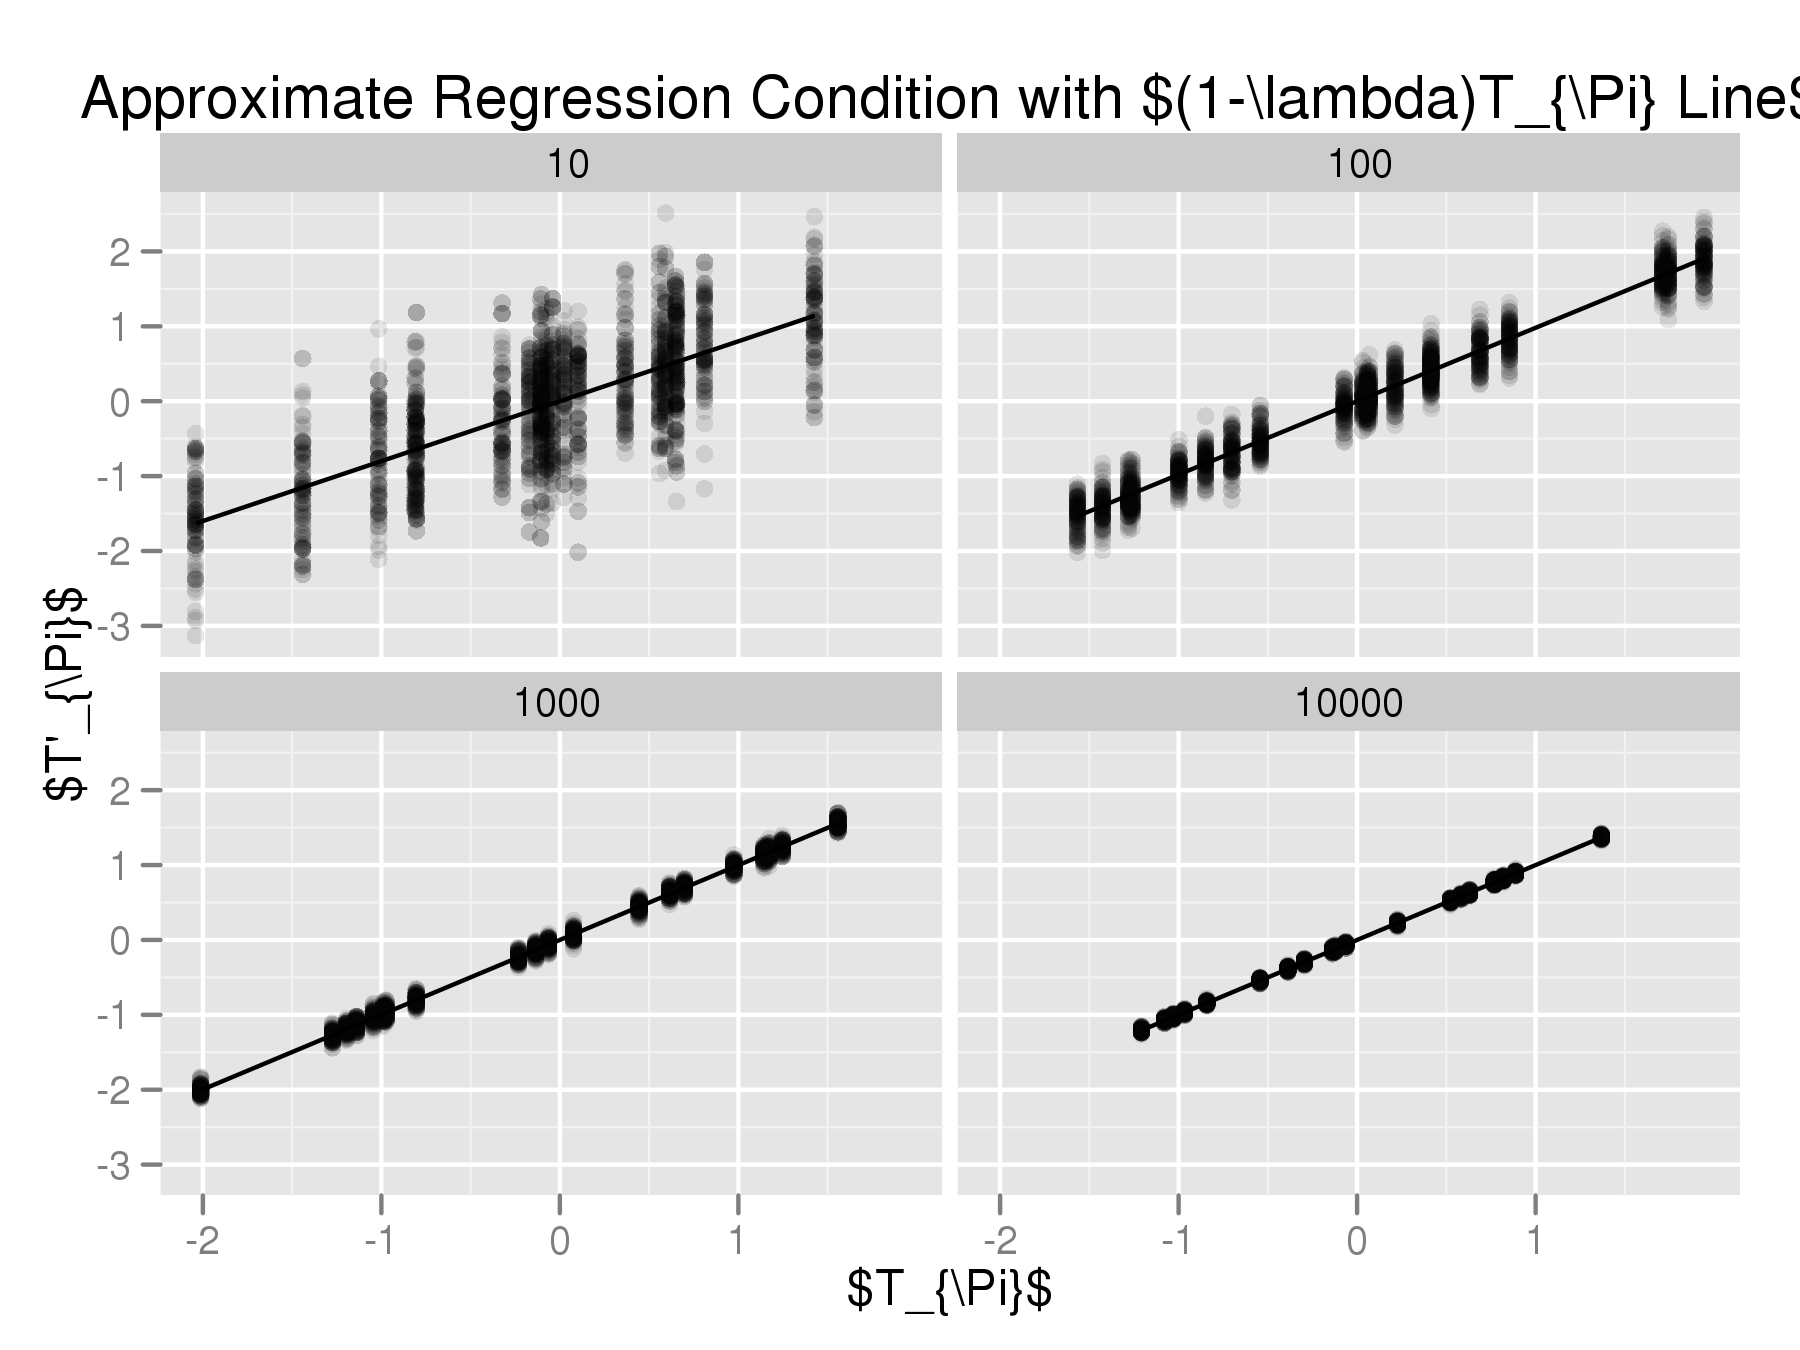
\includegraphics[scale = .75]{./simulations/sim7.png}
  \caption{Faceted on per-group sample size, $N$.}
\end{figure}

The approximate regression condition appears to hold visually.
\clearpage

\section{Main Bounds}
Here we simulate the main bounds under the same setting as the previous section.
\subsection{Failure of Monte Carlo}
Again, we simulate the conditional expectations of the form $\E[f(T'_{\Pi}, T_{\Pi}) | T_{\Pi}]$
with 1,000 draws from the uniform distribution on all group-switching transpositions $(I, J)$.

\begin{figure}[!ht]
  \centering
  % Created by tikzDevice version 0.6.2-92-0ad2792 on 2013-05-05 16:12:43
% !TEX encoding = UTF-8 Unicode
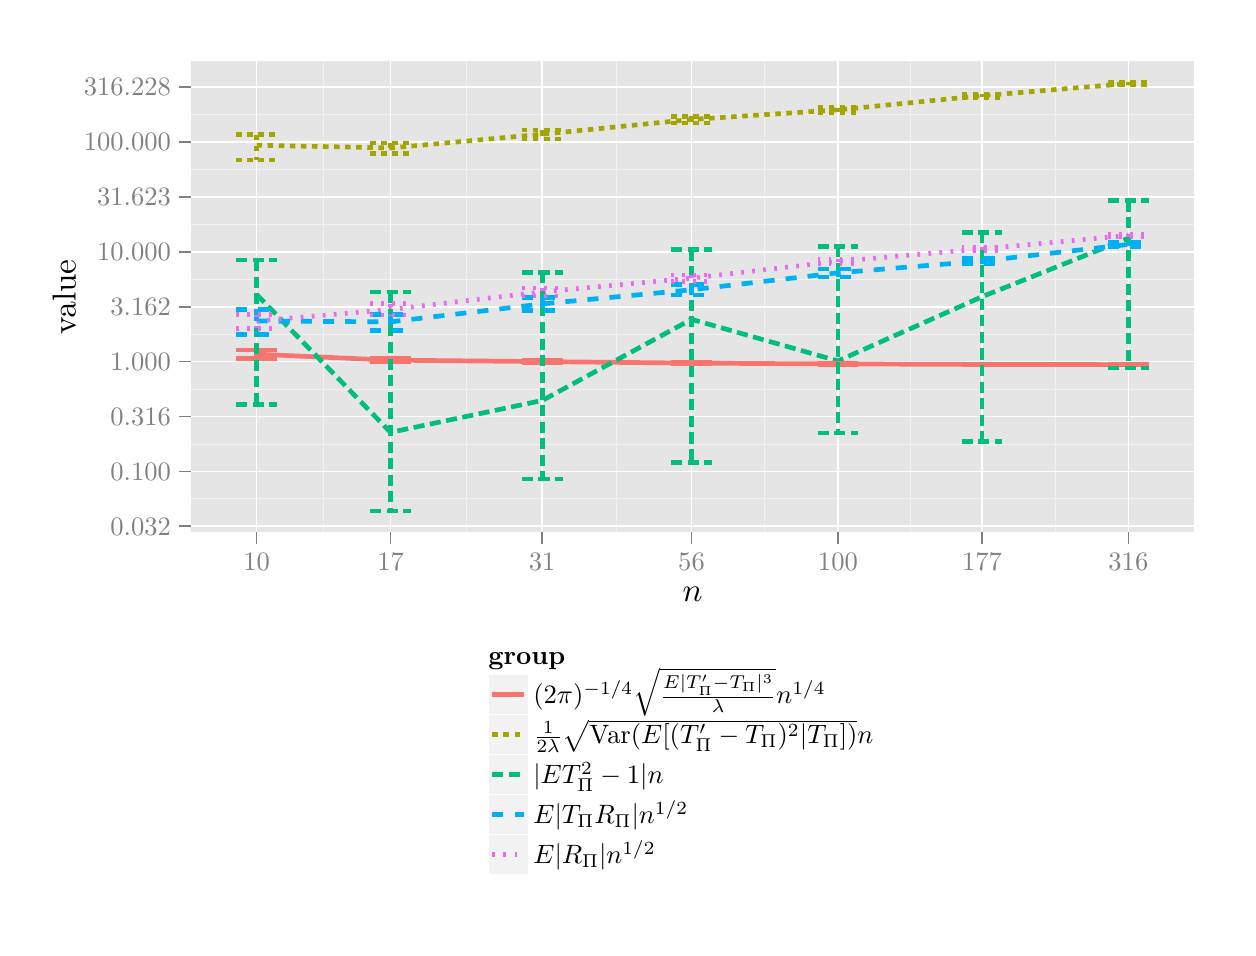
\begin{tikzpicture}[x=1pt,y=1pt]
\definecolor[named]{fillColor}{rgb}{1.00,1.00,1.00}
\path[use as bounding box,fill=fillColor,fill opacity=0.00] (0,0) rectangle (433.62,325.21);
\begin{scope}
\path[clip] (  0.00,  0.00) rectangle (433.62,325.21);
\definecolor[named]{drawColor}{rgb}{1.00,1.00,1.00}
\definecolor[named]{fillColor}{rgb}{1.00,1.00,1.00}

\path[draw=drawColor,line width= 0.6pt,line join=round,line cap=round,fill=fillColor] (  0.00,  0.00) rectangle (433.62,325.21);
\end{scope}
\begin{scope}
\path[clip] ( 58.88,142.81) rectangle (421.57,313.17);
\definecolor[named]{fillColor}{rgb}{0.90,0.90,0.90}

\path[fill=fillColor] ( 58.88,142.81) rectangle (421.57,313.17);
\definecolor[named]{drawColor}{rgb}{0.95,0.95,0.95}

\path[draw=drawColor,line width= 0.3pt,line join=round] ( 58.88,154.98) --
	(421.57,154.98);

\path[draw=drawColor,line width= 0.3pt,line join=round] ( 58.88,174.73) --
	(421.57,174.73);

\path[draw=drawColor,line width= 0.3pt,line join=round] ( 58.88,194.60) --
	(421.57,194.60);

\path[draw=drawColor,line width= 0.3pt,line join=round] ( 58.88,214.46) --
	(421.57,214.46);

\path[draw=drawColor,line width= 0.3pt,line join=round] ( 58.88,234.32) --
	(421.57,234.32);

\path[draw=drawColor,line width= 0.3pt,line join=round] ( 58.88,254.18) --
	(421.57,254.18);

\path[draw=drawColor,line width= 0.3pt,line join=round] ( 58.88,274.04) --
	(421.57,274.04);

\path[draw=drawColor,line width= 0.3pt,line join=round] ( 58.88,293.91) --
	(421.57,293.91);

\path[draw=drawColor,line width= 0.3pt,line join=round] (106.92,142.81) --
	(106.92,313.17);

\path[draw=drawColor,line width= 0.3pt,line join=round] (158.53,142.81) --
	(158.53,313.17);

\path[draw=drawColor,line width= 0.3pt,line join=round] (212.91,142.81) --
	(212.91,313.17);

\path[draw=drawColor,line width= 0.3pt,line join=round] (266.33,142.81) --
	(266.33,313.17);

\path[draw=drawColor,line width= 0.3pt,line join=round] (318.82,142.81) --
	(318.82,313.17);

\path[draw=drawColor,line width= 0.3pt,line join=round] (371.30,142.81) --
	(371.30,313.17);
\definecolor[named]{drawColor}{rgb}{1.00,1.00,1.00}

\path[draw=drawColor,line width= 0.6pt,line join=round] ( 58.88,145.15) --
	(421.57,145.15);

\path[draw=drawColor,line width= 0.6pt,line join=round] ( 58.88,164.81) --
	(421.57,164.81);

\path[draw=drawColor,line width= 0.6pt,line join=round] ( 58.88,184.66) --
	(421.57,184.66);

\path[draw=drawColor,line width= 0.6pt,line join=round] ( 58.88,204.53) --
	(421.57,204.53);

\path[draw=drawColor,line width= 0.6pt,line join=round] ( 58.88,224.39) --
	(421.57,224.39);

\path[draw=drawColor,line width= 0.6pt,line join=round] ( 58.88,244.25) --
	(421.57,244.25);

\path[draw=drawColor,line width= 0.6pt,line join=round] ( 58.88,264.11) --
	(421.57,264.11);

\path[draw=drawColor,line width= 0.6pt,line join=round] ( 58.88,283.97) --
	(421.57,283.97);

\path[draw=drawColor,line width= 0.6pt,line join=round] ( 58.88,303.84) --
	(421.57,303.84);

\path[draw=drawColor,line width= 0.6pt,line join=round] ( 82.72,142.81) --
	( 82.72,313.17);

\path[draw=drawColor,line width= 0.6pt,line join=round] (131.13,142.81) --
	(131.13,313.17);

\path[draw=drawColor,line width= 0.6pt,line join=round] (185.93,142.81) --
	(185.93,313.17);

\path[draw=drawColor,line width= 0.6pt,line join=round] (239.88,142.81) --
	(239.88,313.17);

\path[draw=drawColor,line width= 0.6pt,line join=round] (292.78,142.81) --
	(292.78,313.17);

\path[draw=drawColor,line width= 0.6pt,line join=round] (344.86,142.81) --
	(344.86,313.17);

\path[draw=drawColor,line width= 0.6pt,line join=round] (397.74,142.81) --
	(397.74,313.17);
\definecolor[named]{drawColor}{rgb}{0.97,0.46,0.43}

\path[draw=drawColor,line width= 1.7pt,line join=round] ( 82.72,207.22) --
	(131.13,205.06) --
	(185.93,204.54) --
	(239.88,203.99) --
	(292.78,203.69) --
	(344.86,203.53) --
	(397.74,203.44);
\definecolor[named]{drawColor}{rgb}{0.64,0.65,0.00}

\path[draw=drawColor,line width= 1.7pt,dash pattern=on 2pt off 2pt ,line join=round] ( 82.72,282.74) --
	(131.13,281.74) --
	(185.93,286.71) --
	(239.88,292.04) --
	(292.78,295.51) --
	(344.86,300.63) --
	(397.74,305.03);
\definecolor[named]{drawColor}{rgb}{0.00,0.75,0.49}

\path[draw=drawColor,line width= 1.7pt,dash pattern=on 4pt off 2pt ,line join=round] ( 82.72,228.83) --
	(131.13,178.97) --
	(185.93,190.49) --
	(239.88,219.83) --
	(292.78,204.78) --
	(344.86,227.98) --
	(397.74,249.14);
\definecolor[named]{drawColor}{rgb}{0.00,0.69,0.96}

\path[draw=drawColor,line width= 1.7pt,dash pattern=on 4pt off 4pt ,line join=round] ( 82.72,219.20) --
	(131.13,218.91) --
	(185.93,225.39) --
	(239.88,230.50) --
	(292.78,236.62) --
	(344.86,240.89) --
	(397.74,246.87);
\definecolor[named]{drawColor}{rgb}{0.91,0.42,0.95}

\path[draw=drawColor,line width= 1.7pt,dash pattern=on 1pt off 3pt ,line join=round] ( 82.72,219.21) --
	(131.13,223.37) --
	(185.93,229.76) --
	(239.88,234.70) --
	(292.78,240.75) --
	(344.86,245.25) --
	(397.74,250.15);
\definecolor[named]{drawColor}{rgb}{0.97,0.46,0.43}

\path[draw=drawColor,line width= 1.7pt,line join=round] ( 75.37,208.70) --
	( 90.07,208.70);

\path[draw=drawColor,line width= 1.7pt,line join=round] ( 82.72,208.70) --
	( 82.72,205.69);

\path[draw=drawColor,line width= 1.7pt,line join=round] ( 75.37,205.69) --
	( 90.07,205.69);

\path[draw=drawColor,line width= 1.7pt,line join=round] (123.78,205.74) --
	(138.48,205.74);

\path[draw=drawColor,line width= 1.7pt,line join=round] (131.13,205.74) --
	(131.13,204.43);

\path[draw=drawColor,line width= 1.7pt,line join=round] (123.78,204.43) --
	(138.48,204.43);

\path[draw=drawColor,line width= 1.7pt,line join=round] (178.58,204.92) --
	(193.28,204.92);

\path[draw=drawColor,line width= 1.7pt,line join=round] (185.93,204.92) --
	(185.93,204.16);

\path[draw=drawColor,line width= 1.7pt,line join=round] (178.58,204.16) --
	(193.28,204.16);

\path[draw=drawColor,line width= 1.7pt,line join=round] (232.53,204.22) --
	(247.23,204.22);

\path[draw=drawColor,line width= 1.7pt,line join=round] (239.88,204.22) --
	(239.88,203.78);

\path[draw=drawColor,line width= 1.7pt,line join=round] (232.53,203.78) --
	(247.23,203.78);

\path[draw=drawColor,line width= 1.7pt,line join=round] (285.42,203.81) --
	(300.13,203.81);

\path[draw=drawColor,line width= 1.7pt,line join=round] (292.78,203.81) --
	(292.78,203.59);

\path[draw=drawColor,line width= 1.7pt,line join=round] (285.42,203.59) --
	(300.13,203.59);

\path[draw=drawColor,line width= 1.7pt,line join=round] (337.51,203.60) --
	(352.22,203.60);

\path[draw=drawColor,line width= 1.7pt,line join=round] (344.86,203.60) --
	(344.86,203.47);

\path[draw=drawColor,line width= 1.7pt,line join=round] (337.51,203.47) --
	(352.22,203.47);

\path[draw=drawColor,line width= 1.7pt,line join=round] (390.39,203.48) --
	(405.09,203.48);

\path[draw=drawColor,line width= 1.7pt,line join=round] (397.74,203.48) --
	(397.74,203.40);

\path[draw=drawColor,line width= 1.7pt,line join=round] (390.39,203.40) --
	(405.09,203.40);
\definecolor[named]{drawColor}{rgb}{0.64,0.65,0.00}

\path[draw=drawColor,line width= 1.7pt,dash pattern=on 2pt off 2pt ,line join=round] ( 75.37,286.54) --
	( 90.07,286.54);

\path[draw=drawColor,line width= 1.7pt,dash pattern=on 2pt off 2pt ,line join=round] ( 82.72,286.54) --
	( 82.72,277.38);

\path[draw=drawColor,line width= 1.7pt,dash pattern=on 2pt off 2pt ,line join=round] ( 75.37,277.38) --
	( 90.07,277.38);

\path[draw=drawColor,line width= 1.7pt,dash pattern=on 2pt off 2pt ,line join=round] (123.78,283.55) --
	(138.48,283.55);

\path[draw=drawColor,line width= 1.7pt,dash pattern=on 2pt off 2pt ,line join=round] (131.13,283.55) --
	(131.13,279.65);

\path[draw=drawColor,line width= 1.7pt,dash pattern=on 2pt off 2pt ,line join=round] (123.78,279.65) --
	(138.48,279.65);

\path[draw=drawColor,line width= 1.7pt,dash pattern=on 2pt off 2pt ,line join=round] (178.58,288.22) --
	(193.28,288.22);

\path[draw=drawColor,line width= 1.7pt,dash pattern=on 2pt off 2pt ,line join=round] (185.93,288.22) --
	(185.93,285.03);

\path[draw=drawColor,line width= 1.7pt,dash pattern=on 2pt off 2pt ,line join=round] (178.58,285.03) --
	(193.28,285.03);

\path[draw=drawColor,line width= 1.7pt,dash pattern=on 2pt off 2pt ,line join=round] (232.53,293.18) --
	(247.23,293.18);

\path[draw=drawColor,line width= 1.7pt,dash pattern=on 2pt off 2pt ,line join=round] (239.88,293.18) --
	(239.88,290.76);

\path[draw=drawColor,line width= 1.7pt,dash pattern=on 2pt off 2pt ,line join=round] (232.53,290.76) --
	(247.23,290.76);

\path[draw=drawColor,line width= 1.7pt,dash pattern=on 2pt off 2pt ,line join=round] (285.42,296.28) --
	(300.13,296.28);

\path[draw=drawColor,line width= 1.7pt,dash pattern=on 2pt off 2pt ,line join=round] (292.78,296.28) --
	(292.78,294.66);

\path[draw=drawColor,line width= 1.7pt,dash pattern=on 2pt off 2pt ,line join=round] (285.42,294.66) --
	(300.13,294.66);

\path[draw=drawColor,line width= 1.7pt,dash pattern=on 2pt off 2pt ,line join=round] (337.51,301.23) --
	(352.22,301.23);

\path[draw=drawColor,line width= 1.7pt,dash pattern=on 2pt off 2pt ,line join=round] (344.86,301.23) --
	(344.86,300.04);

\path[draw=drawColor,line width= 1.7pt,dash pattern=on 2pt off 2pt ,line join=round] (337.51,300.04) --
	(352.22,300.04);

\path[draw=drawColor,line width= 1.7pt,dash pattern=on 2pt off 2pt ,line join=round] (390.39,305.43) --
	(405.09,305.43);

\path[draw=drawColor,line width= 1.7pt,dash pattern=on 2pt off 2pt ,line join=round] (397.74,305.43) --
	(397.74,304.62);

\path[draw=drawColor,line width= 1.7pt,dash pattern=on 2pt off 2pt ,line join=round] (390.39,304.62) --
	(405.09,304.62);
\definecolor[named]{drawColor}{rgb}{0.00,0.75,0.49}

\path[draw=drawColor,line width= 1.7pt,dash pattern=on 4pt off 2pt ,line join=round] ( 75.37,241.29) --
	( 90.07,241.29);

\path[draw=drawColor,line width= 1.7pt,dash pattern=on 4pt off 2pt ,line join=round] ( 82.72,241.29) --
	( 82.72,188.99);

\path[draw=drawColor,line width= 1.7pt,dash pattern=on 4pt off 2pt ,line join=round] ( 75.37,188.99) --
	( 90.07,188.99);

\path[draw=drawColor,line width= 1.7pt,dash pattern=on 4pt off 2pt ,line join=round] (123.78,229.66) --
	(138.48,229.66);

\path[draw=drawColor,line width= 1.7pt,dash pattern=on 4pt off 2pt ,line join=round] (131.13,229.66) --
	(131.13,150.56);

\path[draw=drawColor,line width= 1.7pt,dash pattern=on 4pt off 2pt ,line join=round] (123.78,150.56) --
	(138.48,150.56);

\path[draw=drawColor,line width= 1.7pt,dash pattern=on 4pt off 2pt ,line join=round] (178.58,236.84) --
	(193.28,236.84);

\path[draw=drawColor,line width= 1.7pt,dash pattern=on 4pt off 2pt ,line join=round] (185.93,236.84) --
	(185.93,162.12);

\path[draw=drawColor,line width= 1.7pt,dash pattern=on 4pt off 2pt ,line join=round] (178.58,162.12) --
	(193.28,162.12);

\path[draw=drawColor,line width= 1.7pt,dash pattern=on 4pt off 2pt ,line join=round] (232.53,244.94) --
	(247.23,244.94);

\path[draw=drawColor,line width= 1.7pt,dash pattern=on 4pt off 2pt ,line join=round] (239.88,244.94) --
	(239.88,168.10);

\path[draw=drawColor,line width= 1.7pt,dash pattern=on 4pt off 2pt ,line join=round] (232.53,168.10) --
	(247.23,168.10);

\path[draw=drawColor,line width= 1.7pt,dash pattern=on 4pt off 2pt ,line join=round] (285.42,246.23) --
	(300.13,246.23);

\path[draw=drawColor,line width= 1.7pt,dash pattern=on 4pt off 2pt ,line join=round] (292.78,246.23) --
	(292.78,178.72);

\path[draw=drawColor,line width= 1.7pt,dash pattern=on 4pt off 2pt ,line join=round] (285.42,178.72) --
	(300.13,178.72);

\path[draw=drawColor,line width= 1.7pt,dash pattern=on 4pt off 2pt ,line join=round] (337.51,251.29) --
	(352.22,251.29);

\path[draw=drawColor,line width= 1.7pt,dash pattern=on 4pt off 2pt ,line join=round] (344.86,251.29) --
	(344.86,175.75);

\path[draw=drawColor,line width= 1.7pt,dash pattern=on 4pt off 2pt ,line join=round] (337.51,175.75) --
	(352.22,175.75);

\path[draw=drawColor,line width= 1.7pt,dash pattern=on 4pt off 2pt ,line join=round] (390.39,262.73) --
	(405.09,262.73);

\path[draw=drawColor,line width= 1.7pt,dash pattern=on 4pt off 2pt ,line join=round] (397.74,262.73) --
	(397.74,202.27);

\path[draw=drawColor,line width= 1.7pt,dash pattern=on 4pt off 2pt ,line join=round] (390.39,202.27) --
	(405.09,202.27);
\definecolor[named]{drawColor}{rgb}{0.00,0.69,0.96}

\path[draw=drawColor,line width= 1.7pt,dash pattern=on 4pt off 4pt ,line join=round] ( 75.37,223.38) --
	( 90.07,223.38);

\path[draw=drawColor,line width= 1.7pt,dash pattern=on 4pt off 4pt ,line join=round] ( 82.72,223.38) --
	( 82.72,214.35);

\path[draw=drawColor,line width= 1.7pt,dash pattern=on 4pt off 4pt ,line join=round] ( 75.37,214.35) --
	( 90.07,214.35);

\path[draw=drawColor,line width= 1.7pt,dash pattern=on 4pt off 4pt ,line join=round] (123.78,221.64) --
	(138.48,221.64);

\path[draw=drawColor,line width= 1.7pt,dash pattern=on 4pt off 4pt ,line join=round] (131.13,221.64) --
	(131.13,215.68);

\path[draw=drawColor,line width= 1.7pt,dash pattern=on 4pt off 4pt ,line join=round] (123.78,215.68) --
	(138.48,215.68);

\path[draw=drawColor,line width= 1.7pt,dash pattern=on 4pt off 4pt ,line join=round] (178.58,227.78) --
	(193.28,227.78);

\path[draw=drawColor,line width= 1.7pt,dash pattern=on 4pt off 4pt ,line join=round] (185.93,227.78) --
	(185.93,223.08);

\path[draw=drawColor,line width= 1.7pt,dash pattern=on 4pt off 4pt ,line join=round] (178.58,223.08) --
	(193.28,223.08);

\path[draw=drawColor,line width= 1.7pt,dash pattern=on 4pt off 4pt ,line join=round] (232.53,232.39) --
	(247.23,232.39);

\path[draw=drawColor,line width= 1.7pt,dash pattern=on 4pt off 4pt ,line join=round] (239.88,232.39) --
	(239.88,228.59);

\path[draw=drawColor,line width= 1.7pt,dash pattern=on 4pt off 4pt ,line join=round] (232.53,228.59) --
	(247.23,228.59);

\path[draw=drawColor,line width= 1.7pt,dash pattern=on 4pt off 4pt ,line join=round] (285.42,237.99) --
	(300.13,237.99);

\path[draw=drawColor,line width= 1.7pt,dash pattern=on 4pt off 4pt ,line join=round] (292.78,237.99) --
	(292.78,235.14);

\path[draw=drawColor,line width= 1.7pt,dash pattern=on 4pt off 4pt ,line join=round] (285.42,235.14) --
	(300.13,235.14);

\path[draw=drawColor,line width= 1.7pt,dash pattern=on 4pt off 4pt ,line join=round] (337.51,241.85) --
	(352.22,241.85);

\path[draw=drawColor,line width= 1.7pt,dash pattern=on 4pt off 4pt ,line join=round] (344.86,241.85) --
	(344.86,239.90);

\path[draw=drawColor,line width= 1.7pt,dash pattern=on 4pt off 4pt ,line join=round] (337.51,239.90) --
	(352.22,239.90);

\path[draw=drawColor,line width= 1.7pt,dash pattern=on 4pt off 4pt ,line join=round] (390.39,247.57) --
	(405.09,247.57);

\path[draw=drawColor,line width= 1.7pt,dash pattern=on 4pt off 4pt ,line join=round] (397.74,247.57) --
	(397.74,246.14);

\path[draw=drawColor,line width= 1.7pt,dash pattern=on 4pt off 4pt ,line join=round] (390.39,246.14) --
	(405.09,246.14);
\definecolor[named]{drawColor}{rgb}{0.91,0.42,0.95}

\path[draw=drawColor,line width= 1.7pt,dash pattern=on 1pt off 3pt ,line join=round] ( 75.37,221.56) --
	( 90.07,221.56);

\path[draw=drawColor,line width= 1.7pt,dash pattern=on 1pt off 3pt ,line join=round] ( 82.72,221.56) --
	( 82.72,216.44);

\path[draw=drawColor,line width= 1.7pt,dash pattern=on 1pt off 3pt ,line join=round] ( 75.37,216.44) --
	( 90.07,216.44);

\path[draw=drawColor,line width= 1.7pt,dash pattern=on 1pt off 3pt ,line join=round] (123.78,225.43) --
	(138.48,225.43);

\path[draw=drawColor,line width= 1.7pt,dash pattern=on 1pt off 3pt ,line join=round] (131.13,225.43) --
	(131.13,221.38);

\path[draw=drawColor,line width= 1.7pt,dash pattern=on 1pt off 3pt ,line join=round] (123.78,221.38) --
	(138.48,221.38);

\path[draw=drawColor,line width= 1.7pt,dash pattern=on 1pt off 3pt ,line join=round] (178.58,231.14) --
	(193.28,231.14);

\path[draw=drawColor,line width= 1.7pt,dash pattern=on 1pt off 3pt ,line join=round] (185.93,231.14) --
	(185.93,228.27);

\path[draw=drawColor,line width= 1.7pt,dash pattern=on 1pt off 3pt ,line join=round] (178.58,228.27) --
	(193.28,228.27);

\path[draw=drawColor,line width= 1.7pt,dash pattern=on 1pt off 3pt ,line join=round] (232.53,235.79) --
	(247.23,235.79);

\path[draw=drawColor,line width= 1.7pt,dash pattern=on 1pt off 3pt ,line join=round] (239.88,235.79) --
	(239.88,233.61);

\path[draw=drawColor,line width= 1.7pt,dash pattern=on 1pt off 3pt ,line join=round] (232.53,233.61) --
	(247.23,233.61);

\path[draw=drawColor,line width= 1.7pt,dash pattern=on 1pt off 3pt ,line join=round] (285.42,241.57) --
	(300.13,241.57);

\path[draw=drawColor,line width= 1.7pt,dash pattern=on 1pt off 3pt ,line join=round] (292.78,241.57) --
	(292.78,239.92);

\path[draw=drawColor,line width= 1.7pt,dash pattern=on 1pt off 3pt ,line join=round] (285.42,239.92) --
	(300.13,239.92);

\path[draw=drawColor,line width= 1.7pt,dash pattern=on 1pt off 3pt ,line join=round] (337.51,245.84) --
	(352.22,245.84);

\path[draw=drawColor,line width= 1.7pt,dash pattern=on 1pt off 3pt ,line join=round] (344.86,245.84) --
	(344.86,244.68);

\path[draw=drawColor,line width= 1.7pt,dash pattern=on 1pt off 3pt ,line join=round] (337.51,244.68) --
	(352.22,244.68);

\path[draw=drawColor,line width= 1.7pt,dash pattern=on 1pt off 3pt ,line join=round] (390.39,250.59) --
	(405.09,250.59);

\path[draw=drawColor,line width= 1.7pt,dash pattern=on 1pt off 3pt ,line join=round] (397.74,250.59) --
	(397.74,249.67);

\path[draw=drawColor,line width= 1.7pt,dash pattern=on 1pt off 3pt ,line join=round] (390.39,249.67) --
	(405.09,249.67);
\end{scope}
\begin{scope}
\path[clip] (  0.00,  0.00) rectangle (433.62,325.21);
\definecolor[named]{drawColor}{rgb}{0.50,0.50,0.50}

\node[text=drawColor,anchor=base east,inner sep=0pt, outer sep=0pt, scale=  0.96] at ( 51.77,141.85) {0.032};

\node[text=drawColor,anchor=base east,inner sep=0pt, outer sep=0pt, scale=  0.96] at ( 51.77,161.50) {0.100};

\node[text=drawColor,anchor=base east,inner sep=0pt, outer sep=0pt, scale=  0.96] at ( 51.77,181.35) {0.316};

\node[text=drawColor,anchor=base east,inner sep=0pt, outer sep=0pt, scale=  0.96] at ( 51.77,201.23) {1.000};

\node[text=drawColor,anchor=base east,inner sep=0pt, outer sep=0pt, scale=  0.96] at ( 51.77,221.09) {3.162};

\node[text=drawColor,anchor=base east,inner sep=0pt, outer sep=0pt, scale=  0.96] at ( 51.77,240.95) {10.000};

\node[text=drawColor,anchor=base east,inner sep=0pt, outer sep=0pt, scale=  0.96] at ( 51.77,260.81) {31.623};

\node[text=drawColor,anchor=base east,inner sep=0pt, outer sep=0pt, scale=  0.96] at ( 51.77,280.67) {100.000};

\node[text=drawColor,anchor=base east,inner sep=0pt, outer sep=0pt, scale=  0.96] at ( 51.77,300.53) {316.228};
\end{scope}
\begin{scope}
\path[clip] (  0.00,  0.00) rectangle (433.62,325.21);
\definecolor[named]{drawColor}{rgb}{0.50,0.50,0.50}

\path[draw=drawColor,line width= 0.6pt,line join=round] ( 54.61,145.15) --
	( 58.88,145.15);

\path[draw=drawColor,line width= 0.6pt,line join=round] ( 54.61,164.81) --
	( 58.88,164.81);

\path[draw=drawColor,line width= 0.6pt,line join=round] ( 54.61,184.66) --
	( 58.88,184.66);

\path[draw=drawColor,line width= 0.6pt,line join=round] ( 54.61,204.53) --
	( 58.88,204.53);

\path[draw=drawColor,line width= 0.6pt,line join=round] ( 54.61,224.39) --
	( 58.88,224.39);

\path[draw=drawColor,line width= 0.6pt,line join=round] ( 54.61,244.25) --
	( 58.88,244.25);

\path[draw=drawColor,line width= 0.6pt,line join=round] ( 54.61,264.11) --
	( 58.88,264.11);

\path[draw=drawColor,line width= 0.6pt,line join=round] ( 54.61,283.97) --
	( 58.88,283.97);

\path[draw=drawColor,line width= 0.6pt,line join=round] ( 54.61,303.84) --
	( 58.88,303.84);
\end{scope}
\begin{scope}
\path[clip] (  0.00,  0.00) rectangle (433.62,325.21);
\definecolor[named]{drawColor}{rgb}{0.50,0.50,0.50}

\path[draw=drawColor,line width= 0.6pt,line join=round] ( 82.72,138.55) --
	( 82.72,142.81);

\path[draw=drawColor,line width= 0.6pt,line join=round] (131.13,138.55) --
	(131.13,142.81);

\path[draw=drawColor,line width= 0.6pt,line join=round] (185.93,138.55) --
	(185.93,142.81);

\path[draw=drawColor,line width= 0.6pt,line join=round] (239.88,138.55) --
	(239.88,142.81);

\path[draw=drawColor,line width= 0.6pt,line join=round] (292.78,138.55) --
	(292.78,142.81);

\path[draw=drawColor,line width= 0.6pt,line join=round] (344.86,138.55) --
	(344.86,142.81);

\path[draw=drawColor,line width= 0.6pt,line join=round] (397.74,138.55) --
	(397.74,142.81);
\end{scope}
\begin{scope}
\path[clip] (  0.00,  0.00) rectangle (433.62,325.21);
\definecolor[named]{drawColor}{rgb}{0.50,0.50,0.50}

\node[text=drawColor,anchor=base,inner sep=0pt, outer sep=0pt, scale=  0.96] at ( 82.72,129.09) {10};

\node[text=drawColor,anchor=base,inner sep=0pt, outer sep=0pt, scale=  0.96] at (131.13,129.09) {17};

\node[text=drawColor,anchor=base,inner sep=0pt, outer sep=0pt, scale=  0.96] at (185.93,129.09) {31};

\node[text=drawColor,anchor=base,inner sep=0pt, outer sep=0pt, scale=  0.96] at (239.88,129.09) {56};

\node[text=drawColor,anchor=base,inner sep=0pt, outer sep=0pt, scale=  0.96] at (292.78,129.09) {100};

\node[text=drawColor,anchor=base,inner sep=0pt, outer sep=0pt, scale=  0.96] at (344.86,129.09) {177};

\node[text=drawColor,anchor=base,inner sep=0pt, outer sep=0pt, scale=  0.96] at (397.74,129.09) {316};
\end{scope}
\begin{scope}
\path[clip] (  0.00,  0.00) rectangle (433.62,325.21);
\definecolor[named]{drawColor}{rgb}{0.00,0.00,0.00}

\node[text=drawColor,anchor=base,inner sep=0pt, outer sep=0pt, scale=  1.20] at (240.23,117.81) {$n$};
\end{scope}
\begin{scope}
\path[clip] (  0.00,  0.00) rectangle (433.62,325.21);
\definecolor[named]{drawColor}{rgb}{0.00,0.00,0.00}

\node[text=drawColor,rotate= 90.00,anchor=base,inner sep=0pt, outer sep=0pt, scale=  1.20] at ( 17.30,227.99) {value};
\end{scope}
\begin{scope}
\path[clip] (  0.00,  0.00) rectangle (433.62,325.21);
\definecolor[named]{fillColor}{rgb}{1.00,1.00,1.00}

\path[fill=fillColor] (162.21, 14.89) rectangle (318.25,105.93);
\end{scope}
\begin{scope}
\path[clip] (  0.00,  0.00) rectangle (433.62,325.21);
\definecolor[named]{drawColor}{rgb}{0.00,0.00,0.00}

\node[text=drawColor,anchor=base west,inner sep=0pt, outer sep=0pt, scale=  0.96] at (166.47, 95.04) {\bfseries group};
\end{scope}
\begin{scope}
\path[clip] (  0.00,  0.00) rectangle (433.62,325.21);
\definecolor[named]{drawColor}{rgb}{1.00,1.00,1.00}
\definecolor[named]{fillColor}{rgb}{0.95,0.95,0.95}

\path[draw=drawColor,line width= 0.6pt,line join=round,line cap=round,fill=fillColor] (166.47, 76.97) rectangle (180.93, 91.43);
\end{scope}
\begin{scope}
\path[clip] (  0.00,  0.00) rectangle (433.62,325.21);
\definecolor[named]{drawColor}{rgb}{0.97,0.46,0.43}

\path[draw=drawColor,line width= 1.7pt,line join=round] (167.92, 84.20) -- (179.48, 84.20);
\end{scope}
\begin{scope}
\path[clip] (  0.00,  0.00) rectangle (433.62,325.21);
\definecolor[named]{drawColor}{rgb}{0.97,0.46,0.43}

\path[draw=drawColor,line width= 1.7pt,line join=round] (167.92, 84.20) -- (179.48, 84.20);
\end{scope}
\begin{scope}
\path[clip] (  0.00,  0.00) rectangle (433.62,325.21);
\definecolor[named]{drawColor}{rgb}{1.00,1.00,1.00}
\definecolor[named]{fillColor}{rgb}{0.95,0.95,0.95}

\path[draw=drawColor,line width= 0.6pt,line join=round,line cap=round,fill=fillColor] (166.47, 62.52) rectangle (180.93, 76.97);
\end{scope}
\begin{scope}
\path[clip] (  0.00,  0.00) rectangle (433.62,325.21);
\definecolor[named]{drawColor}{rgb}{0.64,0.65,0.00}

\path[draw=drawColor,line width= 1.7pt,dash pattern=on 2pt off 2pt ,line join=round] (167.92, 69.75) -- (179.48, 69.75);
\end{scope}
\begin{scope}
\path[clip] (  0.00,  0.00) rectangle (433.62,325.21);
\definecolor[named]{drawColor}{rgb}{0.64,0.65,0.00}

\path[draw=drawColor,line width= 1.7pt,dash pattern=on 2pt off 2pt ,line join=round] (167.92, 69.75) -- (179.48, 69.75);
\end{scope}
\begin{scope}
\path[clip] (  0.00,  0.00) rectangle (433.62,325.21);
\definecolor[named]{drawColor}{rgb}{1.00,1.00,1.00}
\definecolor[named]{fillColor}{rgb}{0.95,0.95,0.95}

\path[draw=drawColor,line width= 0.6pt,line join=round,line cap=round,fill=fillColor] (166.47, 48.07) rectangle (180.93, 62.52);
\end{scope}
\begin{scope}
\path[clip] (  0.00,  0.00) rectangle (433.62,325.21);
\definecolor[named]{drawColor}{rgb}{0.00,0.75,0.49}

\path[draw=drawColor,line width= 1.7pt,dash pattern=on 4pt off 2pt ,line join=round] (167.92, 55.29) -- (179.48, 55.29);
\end{scope}
\begin{scope}
\path[clip] (  0.00,  0.00) rectangle (433.62,325.21);
\definecolor[named]{drawColor}{rgb}{0.00,0.75,0.49}

\path[draw=drawColor,line width= 1.7pt,dash pattern=on 4pt off 2pt ,line join=round] (167.92, 55.29) -- (179.48, 55.29);
\end{scope}
\begin{scope}
\path[clip] (  0.00,  0.00) rectangle (433.62,325.21);
\definecolor[named]{drawColor}{rgb}{1.00,1.00,1.00}
\definecolor[named]{fillColor}{rgb}{0.95,0.95,0.95}

\path[draw=drawColor,line width= 0.6pt,line join=round,line cap=round,fill=fillColor] (166.47, 33.61) rectangle (180.93, 48.07);
\end{scope}
\begin{scope}
\path[clip] (  0.00,  0.00) rectangle (433.62,325.21);
\definecolor[named]{drawColor}{rgb}{0.00,0.69,0.96}

\path[draw=drawColor,line width= 1.7pt,dash pattern=on 4pt off 4pt ,line join=round] (167.92, 40.84) -- (179.48, 40.84);
\end{scope}
\begin{scope}
\path[clip] (  0.00,  0.00) rectangle (433.62,325.21);
\definecolor[named]{drawColor}{rgb}{0.00,0.69,0.96}

\path[draw=drawColor,line width= 1.7pt,dash pattern=on 4pt off 4pt ,line join=round] (167.92, 40.84) -- (179.48, 40.84);
\end{scope}
\begin{scope}
\path[clip] (  0.00,  0.00) rectangle (433.62,325.21);
\definecolor[named]{drawColor}{rgb}{1.00,1.00,1.00}
\definecolor[named]{fillColor}{rgb}{0.95,0.95,0.95}

\path[draw=drawColor,line width= 0.6pt,line join=round,line cap=round,fill=fillColor] (166.47, 19.16) rectangle (180.93, 33.61);
\end{scope}
\begin{scope}
\path[clip] (  0.00,  0.00) rectangle (433.62,325.21);
\definecolor[named]{drawColor}{rgb}{0.91,0.42,0.95}

\path[draw=drawColor,line width= 1.7pt,dash pattern=on 1pt off 3pt ,line join=round] (167.92, 26.39) -- (179.48, 26.39);
\end{scope}
\begin{scope}
\path[clip] (  0.00,  0.00) rectangle (433.62,325.21);
\definecolor[named]{drawColor}{rgb}{0.91,0.42,0.95}

\path[draw=drawColor,line width= 1.7pt,dash pattern=on 1pt off 3pt ,line join=round] (167.92, 26.39) -- (179.48, 26.39);
\end{scope}
\begin{scope}
\path[clip] (  0.00,  0.00) rectangle (433.62,325.21);
\definecolor[named]{drawColor}{rgb}{0.00,0.00,0.00}

\node[text=drawColor,anchor=base west,inner sep=0pt, outer sep=0pt, scale=  0.96] at (182.73, 80.90) {$(2\pi)^{-1/4}\sqrt{\frac{\mathbb{E}|T'_{\Pi}-T_{\Pi}|^3}{\lambda}}n^{1/4}\quad $};
\end{scope}
\begin{scope}
\path[clip] (  0.00,  0.00) rectangle (433.62,325.21);
\definecolor[named]{drawColor}{rgb}{0.00,0.00,0.00}

\node[text=drawColor,anchor=base west,inner sep=0pt, outer sep=0pt, scale=  0.96] at (182.73, 66.44) {$\frac{1}{2\lambda}\sqrt{\mathrm{Var}(\mathbb{E}[(T'_{\Pi}-T_{\Pi})^2|T_{\Pi}])}n\quad $};
\end{scope}
\begin{scope}
\path[clip] (  0.00,  0.00) rectangle (433.62,325.21);
\definecolor[named]{drawColor}{rgb}{0.00,0.00,0.00}

\node[text=drawColor,anchor=base west,inner sep=0pt, outer sep=0pt, scale=  0.96] at (182.73, 51.99) {$|\mathbb{E}T_{\Pi}^2-1|n\quad $};
\end{scope}
\begin{scope}
\path[clip] (  0.00,  0.00) rectangle (433.62,325.21);
\definecolor[named]{drawColor}{rgb}{0.00,0.00,0.00}

\node[text=drawColor,anchor=base west,inner sep=0pt, outer sep=0pt, scale=  0.96] at (182.73, 37.53) {$\mathbb{E}|T_{\Pi}R_{\Pi}|n^{1/2}\quad $};
\end{scope}
\begin{scope}
\path[clip] (  0.00,  0.00) rectangle (433.62,325.21);
\definecolor[named]{drawColor}{rgb}{0.00,0.00,0.00}

\node[text=drawColor,anchor=base west,inner sep=0pt, outer sep=0pt, scale=  0.96] at (182.73, 23.08) {$\mathbb{E}|R_{\Pi}|n^{1/2}\quad $};
\end{scope}
\end{tikzpicture}

  \caption{Log-log plot of values for each term in the bound,
    simulating the conditional by Monte Carlo.}
\end{figure}
The MC error is too large, and we see some scaled bounds actually increase.
\clearpage

\subsection{Exact Conditional Expectation Calculations}
Here we plot $T'$ for all $N^2$ group-switching transpositions $(I, J)$:
\begin{figure}[!ht]
  \centering
  % Created by tikzDevice version 0.6.2-92-0ad2792 on 2013-03-31 12:41:54
% !TEX encoding = UTF-8 Unicode
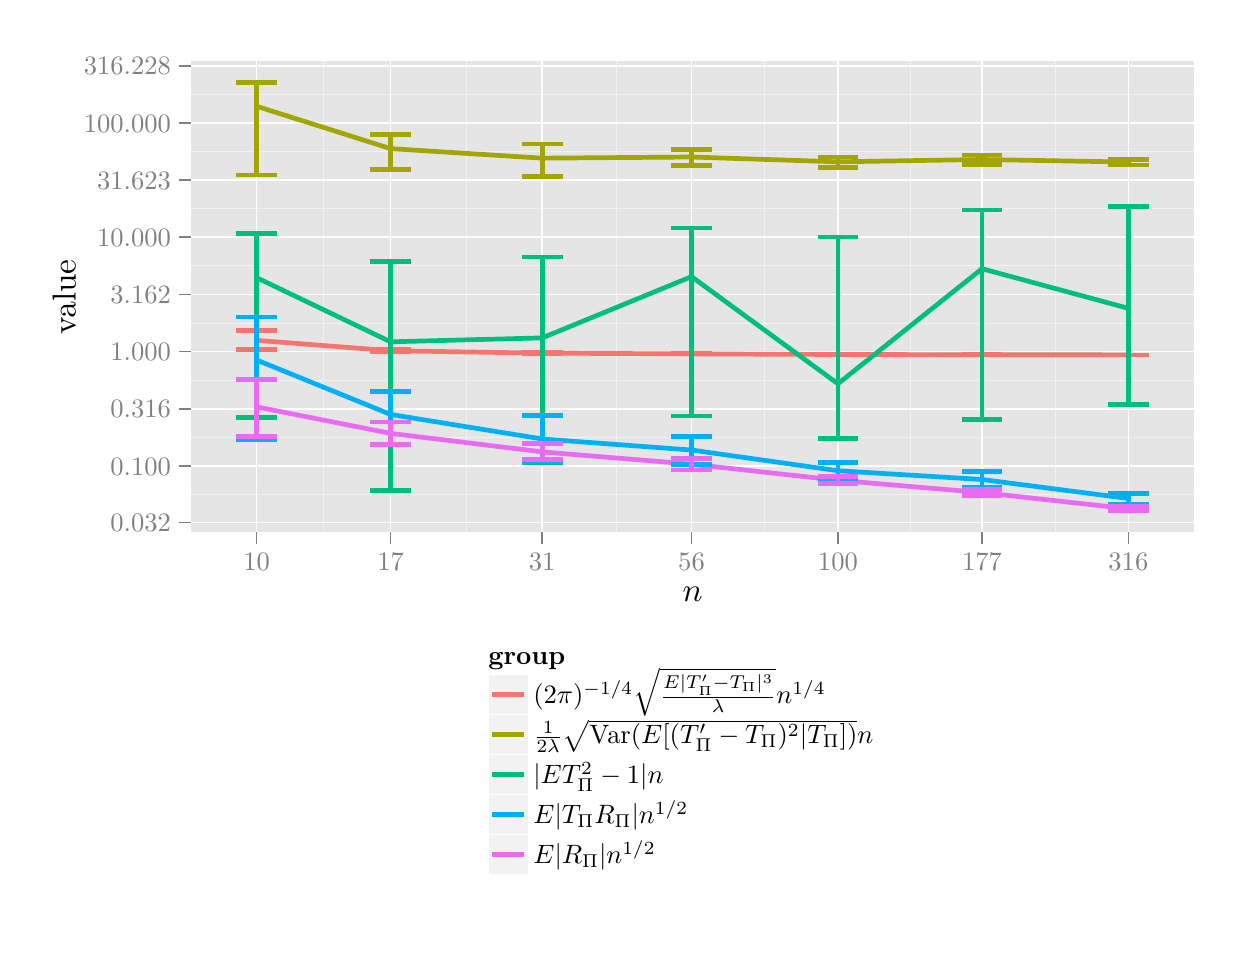
\begin{tikzpicture}[x=1pt,y=1pt]
\definecolor[named]{fillColor}{rgb}{1.00,1.00,1.00}
\path[use as bounding box,fill=fillColor,fill opacity=0.00] (0,0) rectangle (433.62,325.21);
\begin{scope}
\path[clip] (  0.00,  0.00) rectangle (433.62,325.21);
\definecolor[named]{drawColor}{rgb}{1.00,1.00,1.00}
\definecolor[named]{fillColor}{rgb}{1.00,1.00,1.00}

\path[draw=drawColor,line width= 0.6pt,line join=round,line cap=round,fill=fillColor] (  0.00,  0.00) rectangle (433.62,325.21);
\end{scope}
\begin{scope}
\path[clip] ( 58.88,142.81) rectangle (421.57,313.17);
\definecolor[named]{fillColor}{rgb}{0.90,0.90,0.90}

\path[fill=fillColor] ( 58.88,142.81) rectangle (421.57,313.17);
\definecolor[named]{drawColor}{rgb}{0.95,0.95,0.95}

\path[draw=drawColor,line width= 0.3pt,line join=round] ( 58.88,156.64) --
	(421.57,156.64);

\path[draw=drawColor,line width= 0.3pt,line join=round] ( 58.88,177.18) --
	(421.57,177.18);

\path[draw=drawColor,line width= 0.3pt,line join=round] ( 58.88,197.84) --
	(421.57,197.84);

\path[draw=drawColor,line width= 0.3pt,line join=round] ( 58.88,218.50) --
	(421.57,218.50);

\path[draw=drawColor,line width= 0.3pt,line join=round] ( 58.88,239.15) --
	(421.57,239.15);

\path[draw=drawColor,line width= 0.3pt,line join=round] ( 58.88,259.81) --
	(421.57,259.81);

\path[draw=drawColor,line width= 0.3pt,line join=round] ( 58.88,280.46) --
	(421.57,280.46);

\path[draw=drawColor,line width= 0.3pt,line join=round] ( 58.88,301.12) --
	(421.57,301.12);

\path[draw=drawColor,line width= 0.3pt,line join=round] (106.92,142.81) --
	(106.92,313.17);

\path[draw=drawColor,line width= 0.3pt,line join=round] (158.53,142.81) --
	(158.53,313.17);

\path[draw=drawColor,line width= 0.3pt,line join=round] (212.91,142.81) --
	(212.91,313.17);

\path[draw=drawColor,line width= 0.3pt,line join=round] (266.33,142.81) --
	(266.33,313.17);

\path[draw=drawColor,line width= 0.3pt,line join=round] (318.82,142.81) --
	(318.82,313.17);

\path[draw=drawColor,line width= 0.3pt,line join=round] (371.30,142.81) --
	(371.30,313.17);
\definecolor[named]{drawColor}{rgb}{1.00,1.00,1.00}

\path[draw=drawColor,line width= 0.6pt,line join=round] ( 58.88,146.42) --
	(421.57,146.42);

\path[draw=drawColor,line width= 0.6pt,line join=round] ( 58.88,166.86) --
	(421.57,166.86);

\path[draw=drawColor,line width= 0.6pt,line join=round] ( 58.88,187.50) --
	(421.57,187.50);

\path[draw=drawColor,line width= 0.6pt,line join=round] ( 58.88,208.17) --
	(421.57,208.17);

\path[draw=drawColor,line width= 0.6pt,line join=round] ( 58.88,228.82) --
	(421.57,228.82);

\path[draw=drawColor,line width= 0.6pt,line join=round] ( 58.88,249.48) --
	(421.57,249.48);

\path[draw=drawColor,line width= 0.6pt,line join=round] ( 58.88,270.13) --
	(421.57,270.13);

\path[draw=drawColor,line width= 0.6pt,line join=round] ( 58.88,290.79) --
	(421.57,290.79);

\path[draw=drawColor,line width= 0.6pt,line join=round] ( 58.88,311.44) --
	(421.57,311.44);

\path[draw=drawColor,line width= 0.6pt,line join=round] ( 82.72,142.81) --
	( 82.72,313.17);

\path[draw=drawColor,line width= 0.6pt,line join=round] (131.13,142.81) --
	(131.13,313.17);

\path[draw=drawColor,line width= 0.6pt,line join=round] (185.93,142.81) --
	(185.93,313.17);

\path[draw=drawColor,line width= 0.6pt,line join=round] (239.88,142.81) --
	(239.88,313.17);

\path[draw=drawColor,line width= 0.6pt,line join=round] (292.78,142.81) --
	(292.78,313.17);

\path[draw=drawColor,line width= 0.6pt,line join=round] (344.86,142.81) --
	(344.86,313.17);

\path[draw=drawColor,line width= 0.6pt,line join=round] (397.74,142.81) --
	(397.74,313.17);
\definecolor[named]{drawColor}{rgb}{0.97,0.46,0.43}

\path[draw=drawColor,line width= 1.7pt,line join=round] ( 82.72,212.23) --
	(131.13,208.47) --
	(185.93,207.59) --
	(239.88,207.33) --
	(292.78,207.11) --
	(344.86,207.03) --
	(397.74,206.97);
\definecolor[named]{drawColor}{rgb}{0.64,0.65,0.00}

\path[draw=drawColor,line width= 1.7pt,line join=round] ( 82.72,296.81) --
	(131.13,281.50) --
	(185.93,278.05) --
	(239.88,278.47) --
	(292.78,276.73) --
	(344.86,277.57) --
	(397.74,276.65);
\definecolor[named]{drawColor}{rgb}{0.00,0.75,0.49}

\path[draw=drawColor,line width= 1.7pt,line join=round] ( 82.72,234.87) --
	(131.13,211.69) --
	(185.93,213.11) --
	(239.88,235.24) --
	(292.78,196.53) --
	(344.86,238.11) --
	(397.74,223.78);
\definecolor[named]{drawColor}{rgb}{0.00,0.69,0.96}

\path[draw=drawColor,line width= 1.7pt,line join=round] ( 82.72,205.12) --
	(131.13,185.45) --
	(185.93,176.58) --
	(239.88,172.59) --
	(292.78,165.11) --
	(344.86,161.94) --
	(397.74,155.08);
\definecolor[named]{drawColor}{rgb}{0.91,0.42,0.95}

\path[draw=drawColor,line width= 1.7pt,line join=round] ( 82.72,188.19) --
	(131.13,178.60) --
	(185.93,171.91) --
	(239.88,167.48) --
	(292.78,161.66) --
	(344.86,157.21) --
	(397.74,151.36);
\definecolor[named]{drawColor}{rgb}{0.97,0.46,0.43}

\path[draw=drawColor,line width= 1.7pt,line join=round] ( 75.37,215.79) --
	( 90.07,215.79);

\path[draw=drawColor,line width= 1.7pt,line join=round] ( 82.72,215.79) --
	( 82.72,209.03);

\path[draw=drawColor,line width= 1.7pt,line join=round] ( 75.37,209.03) --
	( 90.07,209.03);

\path[draw=drawColor,line width= 1.7pt,line join=round] (123.78,209.01) --
	(138.48,209.01);

\path[draw=drawColor,line width= 1.7pt,line join=round] (131.13,209.01) --
	(131.13,207.96);

\path[draw=drawColor,line width= 1.7pt,line join=round] (123.78,207.96) --
	(138.48,207.96);

\path[draw=drawColor,line width= 1.7pt,line join=round] (178.58,207.78) --
	(193.28,207.78);

\path[draw=drawColor,line width= 1.7pt,line join=round] (185.93,207.78) --
	(185.93,207.43);

\path[draw=drawColor,line width= 1.7pt,line join=round] (178.58,207.43) --
	(193.28,207.43);

\path[draw=drawColor,line width= 1.7pt,line join=round] (232.53,207.40) --
	(247.23,207.40);

\path[draw=drawColor,line width= 1.7pt,line join=round] (239.88,207.40) --
	(239.88,207.26);

\path[draw=drawColor,line width= 1.7pt,line join=round] (232.53,207.26) --
	(247.23,207.26);

\path[draw=drawColor,line width= 1.7pt,line join=round] (285.42,207.14) --
	(300.13,207.14);

\path[draw=drawColor,line width= 1.7pt,line join=round] (292.78,207.14) --
	(292.78,207.09);

\path[draw=drawColor,line width= 1.7pt,line join=round] (285.42,207.09) --
	(300.13,207.09);

\path[draw=drawColor,line width= 1.7pt,line join=round] (337.51,207.04) --
	(352.22,207.04);

\path[draw=drawColor,line width= 1.7pt,line join=round] (344.86,207.04) --
	(344.86,207.01);

\path[draw=drawColor,line width= 1.7pt,line join=round] (337.51,207.01) --
	(352.22,207.01);

\path[draw=drawColor,line width= 1.7pt,line join=round] (390.39,206.98) --
	(405.09,206.98);

\path[draw=drawColor,line width= 1.7pt,line join=round] (397.74,206.98) --
	(397.74,206.97);

\path[draw=drawColor,line width= 1.7pt,line join=round] (390.39,206.97) --
	(405.09,206.97);
\definecolor[named]{drawColor}{rgb}{0.64,0.65,0.00}

\path[draw=drawColor,line width= 1.7pt,line join=round] ( 75.37,305.43) --
	( 90.07,305.43);

\path[draw=drawColor,line width= 1.7pt,line join=round] ( 82.72,305.43) --
	( 82.72,272.00);

\path[draw=drawColor,line width= 1.7pt,line join=round] ( 75.37,272.00) --
	( 90.07,272.00);

\path[draw=drawColor,line width= 1.7pt,line join=round] (123.78,286.57) --
	(138.48,286.57);

\path[draw=drawColor,line width= 1.7pt,line join=round] (131.13,286.57) --
	(131.13,273.88);

\path[draw=drawColor,line width= 1.7pt,line join=round] (123.78,273.88) --
	(138.48,273.88);

\path[draw=drawColor,line width= 1.7pt,line join=round] (178.58,283.20) --
	(193.28,283.20);

\path[draw=drawColor,line width= 1.7pt,line join=round] (185.93,283.20) --
	(185.93,271.44);

\path[draw=drawColor,line width= 1.7pt,line join=round] (178.58,271.44) --
	(193.28,271.44);

\path[draw=drawColor,line width= 1.7pt,line join=round] (232.53,281.15) --
	(247.23,281.15);

\path[draw=drawColor,line width= 1.7pt,line join=round] (239.88,281.15) --
	(239.88,275.41);

\path[draw=drawColor,line width= 1.7pt,line join=round] (232.53,275.41) --
	(247.23,275.41);

\path[draw=drawColor,line width= 1.7pt,line join=round] (285.42,278.48) --
	(300.13,278.48);

\path[draw=drawColor,line width= 1.7pt,line join=round] (292.78,278.48) --
	(292.78,274.78);

\path[draw=drawColor,line width= 1.7pt,line join=round] (285.42,274.78) --
	(300.13,274.78);

\path[draw=drawColor,line width= 1.7pt,line join=round] (337.51,279.20) --
	(352.22,279.20);

\path[draw=drawColor,line width= 1.7pt,line join=round] (344.86,279.20) --
	(344.86,275.70);

\path[draw=drawColor,line width= 1.7pt,line join=round] (337.51,275.70) --
	(352.22,275.70);

\path[draw=drawColor,line width= 1.7pt,line join=round] (390.39,277.66) --
	(405.09,277.66);

\path[draw=drawColor,line width= 1.7pt,line join=round] (397.74,277.66) --
	(397.74,275.55);

\path[draw=drawColor,line width= 1.7pt,line join=round] (390.39,275.55) --
	(405.09,275.55);
\definecolor[named]{drawColor}{rgb}{0.00,0.75,0.49}

\path[draw=drawColor,line width= 1.7pt,line join=round] ( 75.37,250.71) --
	( 90.07,250.71);

\path[draw=drawColor,line width= 1.7pt,line join=round] ( 82.72,250.71) --
	( 82.72,184.35);

\path[draw=drawColor,line width= 1.7pt,line join=round] ( 75.37,184.35) --
	( 90.07,184.35);

\path[draw=drawColor,line width= 1.7pt,line join=round] (123.78,240.65) --
	(138.48,240.65);

\path[draw=drawColor,line width= 1.7pt,line join=round] (131.13,240.65) --
	(131.13,157.85);

\path[draw=drawColor,line width= 1.7pt,line join=round] (123.78,157.85) --
	(138.48,157.85);

\path[draw=drawColor,line width= 1.7pt,line join=round] (178.58,242.36) --
	(193.28,242.36);

\path[draw=drawColor,line width= 1.7pt,line join=round] (185.93,242.36) --
	(185.93,168.02);

\path[draw=drawColor,line width= 1.7pt,line join=round] (178.58,168.02) --
	(193.28,168.02);

\path[draw=drawColor,line width= 1.7pt,line join=round] (232.53,252.82) --
	(247.23,252.82);

\path[draw=drawColor,line width= 1.7pt,line join=round] (239.88,252.82) --
	(239.88,184.90);

\path[draw=drawColor,line width= 1.7pt,line join=round] (232.53,184.90) --
	(247.23,184.90);

\path[draw=drawColor,line width= 1.7pt,line join=round] (285.42,249.54) --
	(300.13,249.54);

\path[draw=drawColor,line width= 1.7pt,line join=round] (292.78,249.54) --
	(292.78,176.72);

\path[draw=drawColor,line width= 1.7pt,line join=round] (285.42,176.72) --
	(300.13,176.72);

\path[draw=drawColor,line width= 1.7pt,line join=round] (337.51,259.28) --
	(352.22,259.28);

\path[draw=drawColor,line width= 1.7pt,line join=round] (344.86,259.28) --
	(344.86,183.59);

\path[draw=drawColor,line width= 1.7pt,line join=round] (337.51,183.59) --
	(352.22,183.59);

\path[draw=drawColor,line width= 1.7pt,line join=round] (390.39,260.67) --
	(405.09,260.67);

\path[draw=drawColor,line width= 1.7pt,line join=round] (397.74,260.67) --
	(397.74,189.01);

\path[draw=drawColor,line width= 1.7pt,line join=round] (390.39,189.01) --
	(405.09,189.01);
\definecolor[named]{drawColor}{rgb}{0.00,0.69,0.96}

\path[draw=drawColor,line width= 1.7pt,line join=round] ( 75.37,220.63) --
	( 90.07,220.63);

\path[draw=drawColor,line width= 1.7pt,line join=round] ( 82.72,220.63) --
	( 82.72,176.45);

\path[draw=drawColor,line width= 1.7pt,line join=round] ( 75.37,176.45) --
	( 90.07,176.45);

\path[draw=drawColor,line width= 1.7pt,line join=round] (123.78,193.86) --
	(138.48,193.86);

\path[draw=drawColor,line width= 1.7pt,line join=round] (131.13,193.86) --
	(131.13,174.67);

\path[draw=drawColor,line width= 1.7pt,line join=round] (123.78,174.67) --
	(138.48,174.67);

\path[draw=drawColor,line width= 1.7pt,line join=round] (178.58,185.02) --
	(193.28,185.02);

\path[draw=drawColor,line width= 1.7pt,line join=round] (185.93,185.02) --
	(185.93,168.34);

\path[draw=drawColor,line width= 1.7pt,line join=round] (178.58,168.34) --
	(193.28,168.34);

\path[draw=drawColor,line width= 1.7pt,line join=round] (232.53,177.45) --
	(247.23,177.45);

\path[draw=drawColor,line width= 1.7pt,line join=round] (239.88,177.45) --
	(239.88,167.34);

\path[draw=drawColor,line width= 1.7pt,line join=round] (232.53,167.34) --
	(247.23,167.34);

\path[draw=drawColor,line width= 1.7pt,line join=round] (285.42,168.13) --
	(300.13,168.13);

\path[draw=drawColor,line width= 1.7pt,line join=round] (292.78,168.13) --
	(292.78,161.90);

\path[draw=drawColor,line width= 1.7pt,line join=round] (285.42,161.90) --
	(300.13,161.90);

\path[draw=drawColor,line width= 1.7pt,line join=round] (337.51,164.95) --
	(352.22,164.95);

\path[draw=drawColor,line width= 1.7pt,line join=round] (344.86,164.95) --
	(344.86,158.98);

\path[draw=drawColor,line width= 1.7pt,line join=round] (337.51,158.98) --
	(352.22,158.98);

\path[draw=drawColor,line width= 1.7pt,line join=round] (390.39,156.99) --
	(405.09,156.99);

\path[draw=drawColor,line width= 1.7pt,line join=round] (397.74,156.99) --
	(397.74,153.12);

\path[draw=drawColor,line width= 1.7pt,line join=round] (390.39,153.12) --
	(405.09,153.12);
\definecolor[named]{drawColor}{rgb}{0.91,0.42,0.95}

\path[draw=drawColor,line width= 1.7pt,line join=round] ( 75.37,198.11) --
	( 90.07,198.11);

\path[draw=drawColor,line width= 1.7pt,line join=round] ( 82.72,198.11) --
	( 82.72,177.60);

\path[draw=drawColor,line width= 1.7pt,line join=round] ( 75.37,177.60) --
	( 90.07,177.60);

\path[draw=drawColor,line width= 1.7pt,line join=round] (123.78,182.73) --
	(138.48,182.73);

\path[draw=drawColor,line width= 1.7pt,line join=round] (131.13,182.73) --
	(131.13,174.52);

\path[draw=drawColor,line width= 1.7pt,line join=round] (123.78,174.52) --
	(138.48,174.52);

\path[draw=drawColor,line width= 1.7pt,line join=round] (178.58,175.06) --
	(193.28,175.06);

\path[draw=drawColor,line width= 1.7pt,line join=round] (185.93,175.06) --
	(185.93,169.10);

\path[draw=drawColor,line width= 1.7pt,line join=round] (178.58,169.10) --
	(193.28,169.10);

\path[draw=drawColor,line width= 1.7pt,line join=round] (232.53,169.53) --
	(247.23,169.53);

\path[draw=drawColor,line width= 1.7pt,line join=round] (239.88,169.53) --
	(239.88,165.42);

\path[draw=drawColor,line width= 1.7pt,line join=round] (232.53,165.42) --
	(247.23,165.42);

\path[draw=drawColor,line width= 1.7pt,line join=round] (285.42,162.96) --
	(300.13,162.96);

\path[draw=drawColor,line width= 1.7pt,line join=round] (292.78,162.96) --
	(292.78,160.37);

\path[draw=drawColor,line width= 1.7pt,line join=round] (285.42,160.37) --
	(300.13,160.37);

\path[draw=drawColor,line width= 1.7pt,line join=round] (337.51,158.45) --
	(352.22,158.45);

\path[draw=drawColor,line width= 1.7pt,line join=round] (344.86,158.45) --
	(344.86,156.04);

\path[draw=drawColor,line width= 1.7pt,line join=round] (337.51,156.04) --
	(352.22,156.04);

\path[draw=drawColor,line width= 1.7pt,line join=round] (390.39,152.16) --
	(405.09,152.16);

\path[draw=drawColor,line width= 1.7pt,line join=round] (397.74,152.16) --
	(397.74,150.56);

\path[draw=drawColor,line width= 1.7pt,line join=round] (390.39,150.56) --
	(405.09,150.56);
\end{scope}
\begin{scope}
\path[clip] (  0.00,  0.00) rectangle (433.62,325.21);
\definecolor[named]{drawColor}{rgb}{0.50,0.50,0.50}

\node[text=drawColor,anchor=base east,inner sep=0pt, outer sep=0pt, scale=  0.96] at ( 51.77,143.11) {0.032};

\node[text=drawColor,anchor=base east,inner sep=0pt, outer sep=0pt, scale=  0.96] at ( 51.77,163.55) {0.100};

\node[text=drawColor,anchor=base east,inner sep=0pt, outer sep=0pt, scale=  0.96] at ( 51.77,184.20) {0.316};

\node[text=drawColor,anchor=base east,inner sep=0pt, outer sep=0pt, scale=  0.96] at ( 51.77,204.86) {1.000};

\node[text=drawColor,anchor=base east,inner sep=0pt, outer sep=0pt, scale=  0.96] at ( 51.77,225.52) {3.162};

\node[text=drawColor,anchor=base east,inner sep=0pt, outer sep=0pt, scale=  0.96] at ( 51.77,246.17) {10.000};

\node[text=drawColor,anchor=base east,inner sep=0pt, outer sep=0pt, scale=  0.96] at ( 51.77,266.83) {31.623};

\node[text=drawColor,anchor=base east,inner sep=0pt, outer sep=0pt, scale=  0.96] at ( 51.77,287.48) {100.000};

\node[text=drawColor,anchor=base east,inner sep=0pt, outer sep=0pt, scale=  0.96] at ( 51.77,308.14) {316.228};
\end{scope}
\begin{scope}
\path[clip] (  0.00,  0.00) rectangle (433.62,325.21);
\definecolor[named]{drawColor}{rgb}{0.50,0.50,0.50}

\path[draw=drawColor,line width= 0.6pt,line join=round] ( 54.61,146.42) --
	( 58.88,146.42);

\path[draw=drawColor,line width= 0.6pt,line join=round] ( 54.61,166.86) --
	( 58.88,166.86);

\path[draw=drawColor,line width= 0.6pt,line join=round] ( 54.61,187.50) --
	( 58.88,187.50);

\path[draw=drawColor,line width= 0.6pt,line join=round] ( 54.61,208.17) --
	( 58.88,208.17);

\path[draw=drawColor,line width= 0.6pt,line join=round] ( 54.61,228.82) --
	( 58.88,228.82);

\path[draw=drawColor,line width= 0.6pt,line join=round] ( 54.61,249.48) --
	( 58.88,249.48);

\path[draw=drawColor,line width= 0.6pt,line join=round] ( 54.61,270.13) --
	( 58.88,270.13);

\path[draw=drawColor,line width= 0.6pt,line join=round] ( 54.61,290.79) --
	( 58.88,290.79);

\path[draw=drawColor,line width= 0.6pt,line join=round] ( 54.61,311.44) --
	( 58.88,311.44);
\end{scope}
\begin{scope}
\path[clip] (  0.00,  0.00) rectangle (433.62,325.21);
\definecolor[named]{drawColor}{rgb}{0.50,0.50,0.50}

\path[draw=drawColor,line width= 0.6pt,line join=round] ( 82.72,138.55) --
	( 82.72,142.81);

\path[draw=drawColor,line width= 0.6pt,line join=round] (131.13,138.55) --
	(131.13,142.81);

\path[draw=drawColor,line width= 0.6pt,line join=round] (185.93,138.55) --
	(185.93,142.81);

\path[draw=drawColor,line width= 0.6pt,line join=round] (239.88,138.55) --
	(239.88,142.81);

\path[draw=drawColor,line width= 0.6pt,line join=round] (292.78,138.55) --
	(292.78,142.81);

\path[draw=drawColor,line width= 0.6pt,line join=round] (344.86,138.55) --
	(344.86,142.81);

\path[draw=drawColor,line width= 0.6pt,line join=round] (397.74,138.55) --
	(397.74,142.81);
\end{scope}
\begin{scope}
\path[clip] (  0.00,  0.00) rectangle (433.62,325.21);
\definecolor[named]{drawColor}{rgb}{0.50,0.50,0.50}

\node[text=drawColor,anchor=base,inner sep=0pt, outer sep=0pt, scale=  0.96] at ( 82.72,129.09) {10};

\node[text=drawColor,anchor=base,inner sep=0pt, outer sep=0pt, scale=  0.96] at (131.13,129.09) {17};

\node[text=drawColor,anchor=base,inner sep=0pt, outer sep=0pt, scale=  0.96] at (185.93,129.09) {31};

\node[text=drawColor,anchor=base,inner sep=0pt, outer sep=0pt, scale=  0.96] at (239.88,129.09) {56};

\node[text=drawColor,anchor=base,inner sep=0pt, outer sep=0pt, scale=  0.96] at (292.78,129.09) {100};

\node[text=drawColor,anchor=base,inner sep=0pt, outer sep=0pt, scale=  0.96] at (344.86,129.09) {177};

\node[text=drawColor,anchor=base,inner sep=0pt, outer sep=0pt, scale=  0.96] at (397.74,129.09) {316};
\end{scope}
\begin{scope}
\path[clip] (  0.00,  0.00) rectangle (433.62,325.21);
\definecolor[named]{drawColor}{rgb}{0.00,0.00,0.00}

\node[text=drawColor,anchor=base,inner sep=0pt, outer sep=0pt, scale=  1.20] at (240.23,117.81) {$n$};
\end{scope}
\begin{scope}
\path[clip] (  0.00,  0.00) rectangle (433.62,325.21);
\definecolor[named]{drawColor}{rgb}{0.00,0.00,0.00}

\node[text=drawColor,rotate= 90.00,anchor=base,inner sep=0pt, outer sep=0pt, scale=  1.20] at ( 17.30,227.99) {value};
\end{scope}
\begin{scope}
\path[clip] (  0.00,  0.00) rectangle (433.62,325.21);
\definecolor[named]{fillColor}{rgb}{1.00,1.00,1.00}

\path[fill=fillColor] (162.21, 14.89) rectangle (318.25,105.93);
\end{scope}
\begin{scope}
\path[clip] (  0.00,  0.00) rectangle (433.62,325.21);
\definecolor[named]{drawColor}{rgb}{0.00,0.00,0.00}

\node[text=drawColor,anchor=base west,inner sep=0pt, outer sep=0pt, scale=  0.96] at (166.47, 95.04) {\bfseries group};
\end{scope}
\begin{scope}
\path[clip] (  0.00,  0.00) rectangle (433.62,325.21);
\definecolor[named]{drawColor}{rgb}{1.00,1.00,1.00}
\definecolor[named]{fillColor}{rgb}{0.95,0.95,0.95}

\path[draw=drawColor,line width= 0.6pt,line join=round,line cap=round,fill=fillColor] (166.47, 76.97) rectangle (180.93, 91.43);
\end{scope}
\begin{scope}
\path[clip] (  0.00,  0.00) rectangle (433.62,325.21);
\definecolor[named]{drawColor}{rgb}{0.97,0.46,0.43}

\path[draw=drawColor,line width= 1.7pt,line join=round] (167.92, 84.20) -- (179.48, 84.20);
\end{scope}
\begin{scope}
\path[clip] (  0.00,  0.00) rectangle (433.62,325.21);
\definecolor[named]{drawColor}{rgb}{0.97,0.46,0.43}

\path[draw=drawColor,line width= 1.7pt,line join=round] (167.92, 84.20) -- (179.48, 84.20);
\end{scope}
\begin{scope}
\path[clip] (  0.00,  0.00) rectangle (433.62,325.21);
\definecolor[named]{drawColor}{rgb}{1.00,1.00,1.00}
\definecolor[named]{fillColor}{rgb}{0.95,0.95,0.95}

\path[draw=drawColor,line width= 0.6pt,line join=round,line cap=round,fill=fillColor] (166.47, 62.52) rectangle (180.93, 76.97);
\end{scope}
\begin{scope}
\path[clip] (  0.00,  0.00) rectangle (433.62,325.21);
\definecolor[named]{drawColor}{rgb}{0.64,0.65,0.00}

\path[draw=drawColor,line width= 1.7pt,line join=round] (167.92, 69.75) -- (179.48, 69.75);
\end{scope}
\begin{scope}
\path[clip] (  0.00,  0.00) rectangle (433.62,325.21);
\definecolor[named]{drawColor}{rgb}{0.64,0.65,0.00}

\path[draw=drawColor,line width= 1.7pt,line join=round] (167.92, 69.75) -- (179.48, 69.75);
\end{scope}
\begin{scope}
\path[clip] (  0.00,  0.00) rectangle (433.62,325.21);
\definecolor[named]{drawColor}{rgb}{1.00,1.00,1.00}
\definecolor[named]{fillColor}{rgb}{0.95,0.95,0.95}

\path[draw=drawColor,line width= 0.6pt,line join=round,line cap=round,fill=fillColor] (166.47, 48.07) rectangle (180.93, 62.52);
\end{scope}
\begin{scope}
\path[clip] (  0.00,  0.00) rectangle (433.62,325.21);
\definecolor[named]{drawColor}{rgb}{0.00,0.75,0.49}

\path[draw=drawColor,line width= 1.7pt,line join=round] (167.92, 55.29) -- (179.48, 55.29);
\end{scope}
\begin{scope}
\path[clip] (  0.00,  0.00) rectangle (433.62,325.21);
\definecolor[named]{drawColor}{rgb}{0.00,0.75,0.49}

\path[draw=drawColor,line width= 1.7pt,line join=round] (167.92, 55.29) -- (179.48, 55.29);
\end{scope}
\begin{scope}
\path[clip] (  0.00,  0.00) rectangle (433.62,325.21);
\definecolor[named]{drawColor}{rgb}{1.00,1.00,1.00}
\definecolor[named]{fillColor}{rgb}{0.95,0.95,0.95}

\path[draw=drawColor,line width= 0.6pt,line join=round,line cap=round,fill=fillColor] (166.47, 33.61) rectangle (180.93, 48.07);
\end{scope}
\begin{scope}
\path[clip] (  0.00,  0.00) rectangle (433.62,325.21);
\definecolor[named]{drawColor}{rgb}{0.00,0.69,0.96}

\path[draw=drawColor,line width= 1.7pt,line join=round] (167.92, 40.84) -- (179.48, 40.84);
\end{scope}
\begin{scope}
\path[clip] (  0.00,  0.00) rectangle (433.62,325.21);
\definecolor[named]{drawColor}{rgb}{0.00,0.69,0.96}

\path[draw=drawColor,line width= 1.7pt,line join=round] (167.92, 40.84) -- (179.48, 40.84);
\end{scope}
\begin{scope}
\path[clip] (  0.00,  0.00) rectangle (433.62,325.21);
\definecolor[named]{drawColor}{rgb}{1.00,1.00,1.00}
\definecolor[named]{fillColor}{rgb}{0.95,0.95,0.95}

\path[draw=drawColor,line width= 0.6pt,line join=round,line cap=round,fill=fillColor] (166.47, 19.16) rectangle (180.93, 33.61);
\end{scope}
\begin{scope}
\path[clip] (  0.00,  0.00) rectangle (433.62,325.21);
\definecolor[named]{drawColor}{rgb}{0.91,0.42,0.95}

\path[draw=drawColor,line width= 1.7pt,line join=round] (167.92, 26.39) -- (179.48, 26.39);
\end{scope}
\begin{scope}
\path[clip] (  0.00,  0.00) rectangle (433.62,325.21);
\definecolor[named]{drawColor}{rgb}{0.91,0.42,0.95}

\path[draw=drawColor,line width= 1.7pt,line join=round] (167.92, 26.39) -- (179.48, 26.39);
\end{scope}
\begin{scope}
\path[clip] (  0.00,  0.00) rectangle (433.62,325.21);
\definecolor[named]{drawColor}{rgb}{0.00,0.00,0.00}

\node[text=drawColor,anchor=base west,inner sep=0pt, outer sep=0pt, scale=  0.96] at (182.73, 80.90) {$(2\pi)^{-1/4}\sqrt{\frac{\mathbb{E}|T'_{\Pi}-T_{\Pi}|^3}{\lambda}}n^{1/4}\quad $};
\end{scope}
\begin{scope}
\path[clip] (  0.00,  0.00) rectangle (433.62,325.21);
\definecolor[named]{drawColor}{rgb}{0.00,0.00,0.00}

\node[text=drawColor,anchor=base west,inner sep=0pt, outer sep=0pt, scale=  0.96] at (182.73, 66.44) {$\frac{1}{2\lambda}\sqrt{\mathrm{Var}(\mathbb{E}[(T'_{\Pi}-T_{\Pi})^2|T_{\Pi}])}n\quad $};
\end{scope}
\begin{scope}
\path[clip] (  0.00,  0.00) rectangle (433.62,325.21);
\definecolor[named]{drawColor}{rgb}{0.00,0.00,0.00}

\node[text=drawColor,anchor=base west,inner sep=0pt, outer sep=0pt, scale=  0.96] at (182.73, 51.99) {$|\mathbb{E}T_{\Pi}^2-1|n\quad $};
\end{scope}
\begin{scope}
\path[clip] (  0.00,  0.00) rectangle (433.62,325.21);
\definecolor[named]{drawColor}{rgb}{0.00,0.00,0.00}

\node[text=drawColor,anchor=base west,inner sep=0pt, outer sep=0pt, scale=  0.96] at (182.73, 37.53) {$\mathbb{E}|T_{\Pi}R_{\Pi}|n^{1/2}\quad $};
\end{scope}
\begin{scope}
\path[clip] (  0.00,  0.00) rectangle (433.62,325.21);
\definecolor[named]{drawColor}{rgb}{0.00,0.00,0.00}

\node[text=drawColor,anchor=base west,inner sep=0pt, outer sep=0pt, scale=  0.96] at (182.73, 23.08) {$\mathbb{E}|R_{\Pi}|n^{1/2}\quad $};
\end{scope}
\end{tikzpicture}

  \caption{Log-log plot of values for each term in the bound, calculating the conditional
    expectation exactly ($10N$ permutations each).}
\end{figure}

Our bounds appear to be of the correct order or slightly conservative in some cases.  The bounds on
the remainder terms ($\E |R_{\Pi}|$ and $\E |T_{\Pi}R_{\Pi}|$) are of order $N^{1/2}$, but the true
rates are probably lower.
\clearpage

\subsection{Better Rate}
\begin{figure}[!ht]
  \centering
  % Created by tikzDevice version 0.6.2-92-0ad2792 on 2013-05-05 16:12:42
% !TEX encoding = UTF-8 Unicode
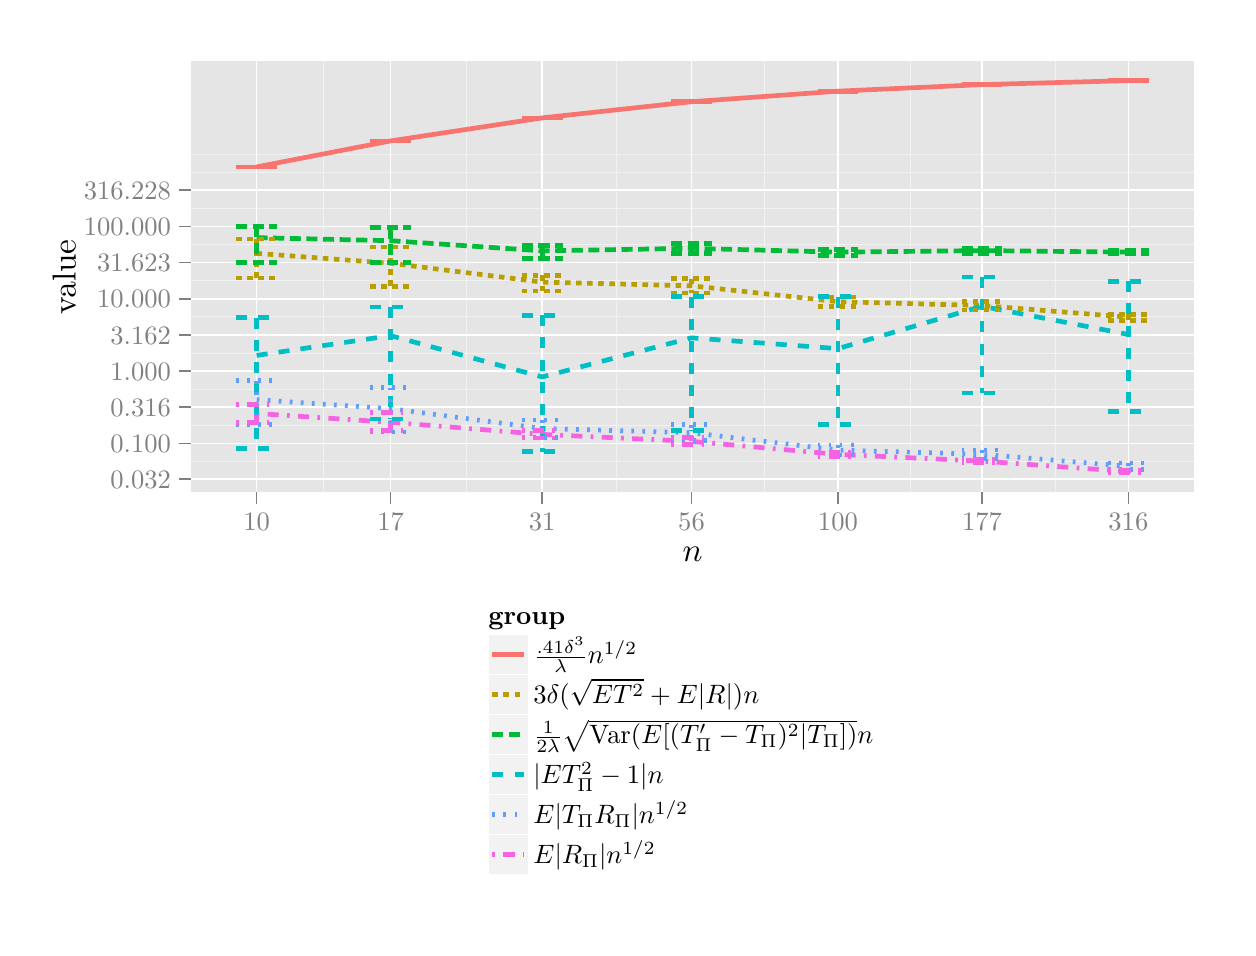
\begin{tikzpicture}[x=1pt,y=1pt]
\definecolor[named]{fillColor}{rgb}{1.00,1.00,1.00}
\path[use as bounding box,fill=fillColor,fill opacity=0.00] (0,0) rectangle (433.62,325.21);
\begin{scope}
\path[clip] (  0.00,  0.00) rectangle (433.62,325.21);
\definecolor[named]{drawColor}{rgb}{1.00,1.00,1.00}
\definecolor[named]{fillColor}{rgb}{1.00,1.00,1.00}

\path[draw=drawColor,line width= 0.6pt,line join=round,line cap=round,fill=fillColor] (  0.00,  0.00) rectangle (433.62,325.21);
\end{scope}
\begin{scope}
\path[clip] ( 58.88,157.27) rectangle (421.57,313.17);
\definecolor[named]{fillColor}{rgb}{0.90,0.90,0.90}

\path[fill=fillColor] ( 58.88,157.27) rectangle (421.57,313.17);
\definecolor[named]{drawColor}{rgb}{0.95,0.95,0.95}

\path[draw=drawColor,line width= 0.3pt,line join=round] ( 58.88,168.50) --
	(421.57,168.50);

\path[draw=drawColor,line width= 0.3pt,line join=round] ( 58.88,181.50) --
	(421.57,181.50);

\path[draw=drawColor,line width= 0.3pt,line join=round] ( 58.88,194.57) --
	(421.57,194.57);

\path[draw=drawColor,line width= 0.3pt,line join=round] ( 58.88,207.64) --
	(421.57,207.64);

\path[draw=drawColor,line width= 0.3pt,line join=round] ( 58.88,220.71) --
	(421.57,220.71);

\path[draw=drawColor,line width= 0.3pt,line join=round] ( 58.88,233.78) --
	(421.57,233.78);

\path[draw=drawColor,line width= 0.3pt,line join=round] ( 58.88,246.85) --
	(421.57,246.85);

\path[draw=drawColor,line width= 0.3pt,line join=round] ( 58.88,259.92) --
	(421.57,259.92);

\path[draw=drawColor,line width= 0.3pt,line join=round] ( 58.88,272.93) --
	(421.57,272.93);

\path[draw=drawColor,line width= 0.3pt,line join=round] ( 58.88,279.39) --
	(421.57,279.39);

\path[draw=drawColor,line width= 0.3pt,line join=round] (106.92,157.27) --
	(106.92,313.17);

\path[draw=drawColor,line width= 0.3pt,line join=round] (158.53,157.27) --
	(158.53,313.17);

\path[draw=drawColor,line width= 0.3pt,line join=round] (212.91,157.27) --
	(212.91,313.17);

\path[draw=drawColor,line width= 0.3pt,line join=round] (266.33,157.27) --
	(266.33,313.17);

\path[draw=drawColor,line width= 0.3pt,line join=round] (318.82,157.27) --
	(318.82,313.17);

\path[draw=drawColor,line width= 0.3pt,line join=round] (371.30,157.27) --
	(371.30,313.17);
\definecolor[named]{drawColor}{rgb}{1.00,1.00,1.00}

\path[draw=drawColor,line width= 0.6pt,line join=round] ( 58.88,162.03) --
	(421.57,162.03);

\path[draw=drawColor,line width= 0.6pt,line join=round] ( 58.88,174.97) --
	(421.57,174.97);

\path[draw=drawColor,line width= 0.6pt,line join=round] ( 58.88,188.03) --
	(421.57,188.03);

\path[draw=drawColor,line width= 0.6pt,line join=round] ( 58.88,201.11) --
	(421.57,201.11);

\path[draw=drawColor,line width= 0.6pt,line join=round] ( 58.88,214.18) --
	(421.57,214.18);

\path[draw=drawColor,line width= 0.6pt,line join=round] ( 58.88,227.25) --
	(421.57,227.25);

\path[draw=drawColor,line width= 0.6pt,line join=round] ( 58.88,240.32) --
	(421.57,240.32);

\path[draw=drawColor,line width= 0.6pt,line join=round] ( 58.88,253.39) --
	(421.57,253.39);

\path[draw=drawColor,line width= 0.6pt,line join=round] ( 58.88,266.46) --
	(421.57,266.46);

\path[draw=drawColor,line width= 0.6pt,line join=round] ( 82.72,157.27) --
	( 82.72,313.17);

\path[draw=drawColor,line width= 0.6pt,line join=round] (131.13,157.27) --
	(131.13,313.17);

\path[draw=drawColor,line width= 0.6pt,line join=round] (185.93,157.27) --
	(185.93,313.17);

\path[draw=drawColor,line width= 0.6pt,line join=round] (239.88,157.27) --
	(239.88,313.17);

\path[draw=drawColor,line width= 0.6pt,line join=round] (292.78,157.27) --
	(292.78,313.17);

\path[draw=drawColor,line width= 0.6pt,line join=round] (344.86,157.27) --
	(344.86,313.17);

\path[draw=drawColor,line width= 0.6pt,line join=round] (397.74,157.27) --
	(397.74,313.17);
\definecolor[named]{drawColor}{rgb}{0.97,0.46,0.43}

\path[draw=drawColor,line width= 1.7pt,line join=round] ( 82.72,274.89) --
	(131.13,284.28) --
	(185.93,292.61) --
	(239.88,298.45) --
	(292.78,302.26) --
	(344.86,304.63) --
	(397.74,306.08);
\definecolor[named]{drawColor}{rgb}{0.72,0.62,0.00}

\path[draw=drawColor,line width= 1.7pt,dash pattern=on 2pt off 2pt ,line join=round] ( 82.72,243.66) --
	(131.13,240.08) --
	(185.93,233.27) --
	(239.88,231.93) --
	(292.78,226.20) --
	(344.86,224.80) --
	(397.74,220.60);
\definecolor[named]{drawColor}{rgb}{0.00,0.73,0.22}

\path[draw=drawColor,line width= 1.7pt,dash pattern=on 4pt off 2pt ,line join=round] ( 82.72,249.33) --
	(131.13,248.23) --
	(185.93,244.56) --
	(239.88,245.48) --
	(292.78,244.09) --
	(344.86,244.65) --
	(397.74,244.10);
\definecolor[named]{drawColor}{rgb}{0.00,0.75,0.77}

\path[draw=drawColor,line width= 1.7pt,dash pattern=on 4pt off 4pt ,line join=round] ( 82.72,206.77) --
	(131.13,213.92) --
	(185.93,199.00) --
	(239.88,213.13) --
	(292.78,209.23) --
	(344.86,224.54) --
	(397.74,214.35);
\definecolor[named]{drawColor}{rgb}{0.38,0.61,1.00}

\path[draw=drawColor,line width= 1.7pt,dash pattern=on 1pt off 3pt ,line join=round] ( 82.72,190.78) --
	(131.13,187.54) --
	(185.93,180.37) --
	(239.88,178.84) --
	(292.78,172.56) --
	(344.86,171.06) --
	(397.74,166.69);
\definecolor[named]{drawColor}{rgb}{0.96,0.39,0.89}

\path[draw=drawColor,line width= 1.7pt,dash pattern=on 1pt off 3pt on 4pt off 3pt ,line join=round] ( 82.72,185.80) --
	(131.13,182.62) --
	(185.93,178.24) --
	(239.88,175.72) --
	(292.78,171.01) --
	(344.86,168.59) --
	(397.74,164.80);
\definecolor[named]{drawColor}{rgb}{0.97,0.46,0.43}

\path[draw=drawColor,line width= 1.7pt,line join=round] ( 75.37,274.89) --
	( 90.07,274.89);

\path[draw=drawColor,line width= 1.7pt,line join=round] ( 82.72,274.89) --
	( 82.72,274.89);

\path[draw=drawColor,line width= 1.7pt,line join=round] ( 75.37,274.89) --
	( 90.07,274.89);

\path[draw=drawColor,line width= 1.7pt,line join=round] (123.78,284.28) --
	(138.48,284.28);

\path[draw=drawColor,line width= 1.7pt,line join=round] (131.13,284.28) --
	(131.13,284.28);

\path[draw=drawColor,line width= 1.7pt,line join=round] (123.78,284.28) --
	(138.48,284.28);

\path[draw=drawColor,line width= 1.7pt,line join=round] (178.58,292.61) --
	(193.28,292.61);

\path[draw=drawColor,line width= 1.7pt,line join=round] (185.93,292.61) --
	(185.93,292.61);

\path[draw=drawColor,line width= 1.7pt,line join=round] (178.58,292.61) --
	(193.28,292.61);

\path[draw=drawColor,line width= 1.7pt,line join=round] (232.53,298.45) --
	(247.23,298.45);

\path[draw=drawColor,line width= 1.7pt,line join=round] (239.88,298.45) --
	(239.88,298.45);

\path[draw=drawColor,line width= 1.7pt,line join=round] (232.53,298.45) --
	(247.23,298.45);

\path[draw=drawColor,line width= 1.7pt,line join=round] (285.42,302.26) --
	(300.13,302.26);

\path[draw=drawColor,line width= 1.7pt,line join=round] (292.78,302.26) --
	(292.78,302.26);

\path[draw=drawColor,line width= 1.7pt,line join=round] (285.42,302.26) --
	(300.13,302.26);

\path[draw=drawColor,line width= 1.7pt,line join=round] (337.51,304.63) --
	(352.22,304.63);

\path[draw=drawColor,line width= 1.7pt,line join=round] (344.86,304.63) --
	(344.86,304.63);

\path[draw=drawColor,line width= 1.7pt,line join=round] (337.51,304.63) --
	(352.22,304.63);

\path[draw=drawColor,line width= 1.7pt,line join=round] (390.39,306.08) --
	(405.09,306.08);

\path[draw=drawColor,line width= 1.7pt,line join=round] (397.74,306.08) --
	(397.74,306.08);

\path[draw=drawColor,line width= 1.7pt,line join=round] (390.39,306.08) --
	(405.09,306.08);
\definecolor[named]{drawColor}{rgb}{0.72,0.62,0.00}

\path[draw=drawColor,line width= 1.7pt,dash pattern=on 2pt off 2pt ,line join=round] ( 75.37,248.87) --
	( 90.07,248.87);

\path[draw=drawColor,line width= 1.7pt,dash pattern=on 2pt off 2pt ,line join=round] ( 82.72,248.87) --
	( 82.72,234.74);

\path[draw=drawColor,line width= 1.7pt,dash pattern=on 2pt off 2pt ,line join=round] ( 75.37,234.74) --
	( 90.07,234.74);

\path[draw=drawColor,line width= 1.7pt,dash pattern=on 2pt off 2pt ,line join=round] (123.78,245.97) --
	(138.48,245.97);

\path[draw=drawColor,line width= 1.7pt,dash pattern=on 2pt off 2pt ,line join=round] (131.13,245.97) --
	(131.13,231.80);

\path[draw=drawColor,line width= 1.7pt,dash pattern=on 2pt off 2pt ,line join=round] (123.78,231.80) --
	(138.48,231.80);

\path[draw=drawColor,line width= 1.7pt,dash pattern=on 2pt off 2pt ,line join=round] (178.58,235.77) --
	(193.28,235.77);

\path[draw=drawColor,line width= 1.7pt,dash pattern=on 2pt off 2pt ,line join=round] (185.93,235.77) --
	(185.93,230.09);

\path[draw=drawColor,line width= 1.7pt,dash pattern=on 2pt off 2pt ,line join=round] (178.58,230.09) --
	(193.28,230.09);

\path[draw=drawColor,line width= 1.7pt,dash pattern=on 2pt off 2pt ,line join=round] (232.53,234.49) --
	(247.23,234.49);

\path[draw=drawColor,line width= 1.7pt,dash pattern=on 2pt off 2pt ,line join=round] (239.88,234.49) --
	(239.88,229.34);

\path[draw=drawColor,line width= 1.7pt,dash pattern=on 2pt off 2pt ,line join=round] (232.53,229.34) --
	(247.23,229.34);

\path[draw=drawColor,line width= 1.7pt,dash pattern=on 2pt off 2pt ,line join=round] (285.42,227.86) --
	(300.13,227.86);

\path[draw=drawColor,line width= 1.7pt,dash pattern=on 2pt off 2pt ,line join=round] (292.78,227.86) --
	(292.78,224.41);

\path[draw=drawColor,line width= 1.7pt,dash pattern=on 2pt off 2pt ,line join=round] (285.42,224.41) --
	(300.13,224.41);

\path[draw=drawColor,line width= 1.7pt,dash pattern=on 2pt off 2pt ,line join=round] (337.51,226.29) --
	(352.22,226.29);

\path[draw=drawColor,line width= 1.7pt,dash pattern=on 2pt off 2pt ,line join=round] (344.86,226.29) --
	(344.86,223.23);

\path[draw=drawColor,line width= 1.7pt,dash pattern=on 2pt off 2pt ,line join=round] (337.51,223.23) --
	(352.22,223.23);

\path[draw=drawColor,line width= 1.7pt,dash pattern=on 2pt off 2pt ,line join=round] (390.39,221.68) --
	(405.09,221.68);

\path[draw=drawColor,line width= 1.7pt,dash pattern=on 2pt off 2pt ,line join=round] (397.74,221.68) --
	(397.74,219.48);

\path[draw=drawColor,line width= 1.7pt,dash pattern=on 2pt off 2pt ,line join=round] (390.39,219.48) --
	(405.09,219.48);
\definecolor[named]{drawColor}{rgb}{0.00,0.73,0.22}

\path[draw=drawColor,line width= 1.7pt,dash pattern=on 4pt off 2pt ,line join=round] ( 75.37,253.42) --
	( 90.07,253.42);

\path[draw=drawColor,line width= 1.7pt,dash pattern=on 4pt off 2pt ,line join=round] ( 82.72,253.42) --
	( 82.72,240.31);

\path[draw=drawColor,line width= 1.7pt,dash pattern=on 4pt off 2pt ,line join=round] ( 75.37,240.31) --
	( 90.07,240.31);

\path[draw=drawColor,line width= 1.7pt,dash pattern=on 4pt off 2pt ,line join=round] (123.78,252.95) --
	(138.48,252.95);

\path[draw=drawColor,line width= 1.7pt,dash pattern=on 4pt off 2pt ,line join=round] (131.13,252.95) --
	(131.13,240.33);

\path[draw=drawColor,line width= 1.7pt,dash pattern=on 4pt off 2pt ,line join=round] (123.78,240.33) --
	(138.48,240.33);

\path[draw=drawColor,line width= 1.7pt,dash pattern=on 4pt off 2pt ,line join=round] (178.58,246.46) --
	(193.28,246.46);

\path[draw=drawColor,line width= 1.7pt,dash pattern=on 4pt off 2pt ,line join=round] (185.93,246.46) --
	(185.93,241.88);

\path[draw=drawColor,line width= 1.7pt,dash pattern=on 4pt off 2pt ,line join=round] (178.58,241.88) --
	(193.28,241.88);

\path[draw=drawColor,line width= 1.7pt,dash pattern=on 4pt off 2pt ,line join=round] (232.53,247.11) --
	(247.23,247.11);

\path[draw=drawColor,line width= 1.7pt,dash pattern=on 4pt off 2pt ,line join=round] (239.88,247.11) --
	(239.88,243.71);

\path[draw=drawColor,line width= 1.7pt,dash pattern=on 4pt off 2pt ,line join=round] (232.53,243.71) --
	(247.23,243.71);

\path[draw=drawColor,line width= 1.7pt,dash pattern=on 4pt off 2pt ,line join=round] (285.42,245.16) --
	(300.13,245.16);

\path[draw=drawColor,line width= 1.7pt,dash pattern=on 4pt off 2pt ,line join=round] (292.78,245.16) --
	(292.78,242.89);

\path[draw=drawColor,line width= 1.7pt,dash pattern=on 4pt off 2pt ,line join=round] (285.42,242.89) --
	(300.13,242.89);

\path[draw=drawColor,line width= 1.7pt,dash pattern=on 4pt off 2pt ,line join=round] (337.51,245.53) --
	(352.22,245.53);

\path[draw=drawColor,line width= 1.7pt,dash pattern=on 4pt off 2pt ,line join=round] (344.86,245.53) --
	(344.86,243.65);

\path[draw=drawColor,line width= 1.7pt,dash pattern=on 4pt off 2pt ,line join=round] (337.51,243.65) --
	(352.22,243.65);

\path[draw=drawColor,line width= 1.7pt,dash pattern=on 4pt off 2pt ,line join=round] (390.39,244.74) --
	(405.09,244.74);

\path[draw=drawColor,line width= 1.7pt,dash pattern=on 4pt off 2pt ,line join=round] (397.74,244.74) --
	(397.74,243.44);

\path[draw=drawColor,line width= 1.7pt,dash pattern=on 4pt off 2pt ,line join=round] (390.39,243.44) --
	(405.09,243.44);
\definecolor[named]{drawColor}{rgb}{0.00,0.75,0.77}

\path[draw=drawColor,line width= 1.7pt,dash pattern=on 4pt off 4pt ,line join=round] ( 75.37,220.42) --
	( 90.07,220.42);

\path[draw=drawColor,line width= 1.7pt,dash pattern=on 4pt off 4pt ,line join=round] ( 82.72,220.42) --
	( 82.72,173.09);

\path[draw=drawColor,line width= 1.7pt,dash pattern=on 4pt off 4pt ,line join=round] ( 75.37,173.09) --
	( 90.07,173.09);

\path[draw=drawColor,line width= 1.7pt,dash pattern=on 4pt off 4pt ,line join=round] (123.78,224.22) --
	(138.48,224.22);

\path[draw=drawColor,line width= 1.7pt,dash pattern=on 4pt off 4pt ,line join=round] (131.13,224.22) --
	(131.13,183.80);

\path[draw=drawColor,line width= 1.7pt,dash pattern=on 4pt off 4pt ,line join=round] (123.78,183.80) --
	(138.48,183.80);

\path[draw=drawColor,line width= 1.7pt,dash pattern=on 4pt off 4pt ,line join=round] (178.58,221.29) --
	(193.28,221.29);

\path[draw=drawColor,line width= 1.7pt,dash pattern=on 4pt off 4pt ,line join=round] (185.93,221.29) --
	(185.93,172.02);

\path[draw=drawColor,line width= 1.7pt,dash pattern=on 4pt off 4pt ,line join=round] (178.58,172.02) --
	(193.28,172.02);

\path[draw=drawColor,line width= 1.7pt,dash pattern=on 4pt off 4pt ,line join=round] (232.53,228.00) --
	(247.23,228.00);

\path[draw=drawColor,line width= 1.7pt,dash pattern=on 4pt off 4pt ,line join=round] (239.88,228.00) --
	(239.88,179.75);

\path[draw=drawColor,line width= 1.7pt,dash pattern=on 4pt off 4pt ,line join=round] (232.53,179.75) --
	(247.23,179.75);

\path[draw=drawColor,line width= 1.7pt,dash pattern=on 4pt off 4pt ,line join=round] (285.42,228.02) --
	(300.13,228.02);

\path[draw=drawColor,line width= 1.7pt,dash pattern=on 4pt off 4pt ,line join=round] (292.78,228.02) --
	(292.78,181.91);

\path[draw=drawColor,line width= 1.7pt,dash pattern=on 4pt off 4pt ,line join=round] (285.42,181.91) --
	(300.13,181.91);

\path[draw=drawColor,line width= 1.7pt,dash pattern=on 4pt off 4pt ,line join=round] (337.51,235.07) --
	(352.22,235.07);

\path[draw=drawColor,line width= 1.7pt,dash pattern=on 4pt off 4pt ,line join=round] (344.86,235.07) --
	(344.86,193.17);

\path[draw=drawColor,line width= 1.7pt,dash pattern=on 4pt off 4pt ,line join=round] (337.51,193.17) --
	(352.22,193.17);

\path[draw=drawColor,line width= 1.7pt,dash pattern=on 4pt off 4pt ,line join=round] (390.39,233.58) --
	(405.09,233.58);

\path[draw=drawColor,line width= 1.7pt,dash pattern=on 4pt off 4pt ,line join=round] (397.74,233.58) --
	(397.74,186.61);

\path[draw=drawColor,line width= 1.7pt,dash pattern=on 4pt off 4pt ,line join=round] (390.39,186.61) --
	(405.09,186.61);
\definecolor[named]{drawColor}{rgb}{0.38,0.61,1.00}

\path[draw=drawColor,line width= 1.7pt,dash pattern=on 1pt off 3pt ,line join=round] ( 75.37,197.61) --
	( 90.07,197.61);

\path[draw=drawColor,line width= 1.7pt,dash pattern=on 1pt off 3pt ,line join=round] ( 82.72,197.61) --
	( 82.72,181.75);

\path[draw=drawColor,line width= 1.7pt,dash pattern=on 1pt off 3pt ,line join=round] ( 75.37,181.75) --
	( 90.07,181.75);

\path[draw=drawColor,line width= 1.7pt,dash pattern=on 1pt off 3pt ,line join=round] (123.78,195.10) --
	(138.48,195.10);

\path[draw=drawColor,line width= 1.7pt,dash pattern=on 1pt off 3pt ,line join=round] (131.13,195.10) --
	(131.13,179.14);

\path[draw=drawColor,line width= 1.7pt,dash pattern=on 1pt off 3pt ,line join=round] (123.78,179.14) --
	(138.48,179.14);

\path[draw=drawColor,line width= 1.7pt,dash pattern=on 1pt off 3pt ,line join=round] (178.58,183.39) --
	(193.28,183.39);

\path[draw=drawColor,line width= 1.7pt,dash pattern=on 1pt off 3pt ,line join=round] (185.93,183.39) --
	(185.93,177.06);

\path[draw=drawColor,line width= 1.7pt,dash pattern=on 1pt off 3pt ,line join=round] (178.58,177.06) --
	(193.28,177.06);

\path[draw=drawColor,line width= 1.7pt,dash pattern=on 1pt off 3pt ,line join=round] (232.53,181.72) --
	(247.23,181.72);

\path[draw=drawColor,line width= 1.7pt,dash pattern=on 1pt off 3pt ,line join=round] (239.88,181.72) --
	(239.88,176.01);

\path[draw=drawColor,line width= 1.7pt,dash pattern=on 1pt off 3pt ,line join=round] (232.53,176.01) --
	(247.23,176.01);

\path[draw=drawColor,line width= 1.7pt,dash pattern=on 1pt off 3pt ,line join=round] (285.42,174.38) --
	(300.13,174.38);

\path[draw=drawColor,line width= 1.7pt,dash pattern=on 1pt off 3pt ,line join=round] (292.78,174.38) --
	(292.78,170.76);

\path[draw=drawColor,line width= 1.7pt,dash pattern=on 1pt off 3pt ,line join=round] (285.42,170.76) --
	(300.13,170.76);

\path[draw=drawColor,line width= 1.7pt,dash pattern=on 1pt off 3pt ,line join=round] (337.51,172.65) --
	(352.22,172.65);

\path[draw=drawColor,line width= 1.7pt,dash pattern=on 1pt off 3pt ,line join=round] (344.86,172.65) --
	(344.86,169.46);

\path[draw=drawColor,line width= 1.7pt,dash pattern=on 1pt off 3pt ,line join=round] (337.51,169.46) --
	(352.22,169.46);

\path[draw=drawColor,line width= 1.7pt,dash pattern=on 1pt off 3pt ,line join=round] (390.39,167.90) --
	(405.09,167.90);

\path[draw=drawColor,line width= 1.7pt,dash pattern=on 1pt off 3pt ,line join=round] (397.74,167.90) --
	(397.74,165.53);

\path[draw=drawColor,line width= 1.7pt,dash pattern=on 1pt off 3pt ,line join=round] (390.39,165.53) --
	(405.09,165.53);
\definecolor[named]{drawColor}{rgb}{0.96,0.39,0.89}

\path[draw=drawColor,line width= 1.7pt,dash pattern=on 1pt off 3pt on 4pt off 3pt ,line join=round] ( 75.37,189.04) --
	( 90.07,189.04);

\path[draw=drawColor,line width= 1.7pt,dash pattern=on 1pt off 3pt on 4pt off 3pt ,line join=round] ( 82.72,189.04) --
	( 82.72,182.53);

\path[draw=drawColor,line width= 1.7pt,dash pattern=on 1pt off 3pt on 4pt off 3pt ,line join=round] ( 75.37,182.53) --
	( 90.07,182.53);

\path[draw=drawColor,line width= 1.7pt,dash pattern=on 1pt off 3pt on 4pt off 3pt ,line join=round] (123.78,186.20) --
	(138.48,186.20);

\path[draw=drawColor,line width= 1.7pt,dash pattern=on 1pt off 3pt on 4pt off 3pt ,line join=round] (131.13,186.20) --
	(131.13,179.73);

\path[draw=drawColor,line width= 1.7pt,dash pattern=on 1pt off 3pt on 4pt off 3pt ,line join=round] (123.78,179.73) --
	(138.48,179.73);

\path[draw=drawColor,line width= 1.7pt,dash pattern=on 1pt off 3pt on 4pt off 3pt ,line join=round] (178.58,179.63) --
	(193.28,179.63);

\path[draw=drawColor,line width= 1.7pt,dash pattern=on 1pt off 3pt on 4pt off 3pt ,line join=round] (185.93,179.63) --
	(185.93,176.94);

\path[draw=drawColor,line width= 1.7pt,dash pattern=on 1pt off 3pt on 4pt off 3pt ,line join=round] (178.58,176.94) --
	(193.28,176.94);

\path[draw=drawColor,line width= 1.7pt,dash pattern=on 1pt off 3pt on 4pt off 3pt ,line join=round] (232.53,176.99) --
	(247.23,176.99);

\path[draw=drawColor,line width= 1.7pt,dash pattern=on 1pt off 3pt on 4pt off 3pt ,line join=round] (239.88,176.99) --
	(239.88,174.54);

\path[draw=drawColor,line width= 1.7pt,dash pattern=on 1pt off 3pt on 4pt off 3pt ,line join=round] (232.53,174.54) --
	(247.23,174.54);

\path[draw=drawColor,line width= 1.7pt,dash pattern=on 1pt off 3pt on 4pt off 3pt ,line join=round] (285.42,171.79) --
	(300.13,171.79);

\path[draw=drawColor,line width= 1.7pt,dash pattern=on 1pt off 3pt on 4pt off 3pt ,line join=round] (292.78,171.79) --
	(292.78,170.31);

\path[draw=drawColor,line width= 1.7pt,dash pattern=on 1pt off 3pt on 4pt off 3pt ,line join=round] (285.42,170.31) --
	(300.13,170.31);

\path[draw=drawColor,line width= 1.7pt,dash pattern=on 1pt off 3pt on 4pt off 3pt ,line join=round] (337.51,169.29) --
	(352.22,169.29);

\path[draw=drawColor,line width= 1.7pt,dash pattern=on 1pt off 3pt on 4pt off 3pt ,line join=round] (344.86,169.29) --
	(344.86,167.97);

\path[draw=drawColor,line width= 1.7pt,dash pattern=on 1pt off 3pt on 4pt off 3pt ,line join=round] (337.51,167.97) --
	(352.22,167.97);

\path[draw=drawColor,line width= 1.7pt,dash pattern=on 1pt off 3pt on 4pt off 3pt ,line join=round] (390.39,165.25) --
	(405.09,165.25);

\path[draw=drawColor,line width= 1.7pt,dash pattern=on 1pt off 3pt on 4pt off 3pt ,line join=round] (397.74,165.25) --
	(397.74,164.35);

\path[draw=drawColor,line width= 1.7pt,dash pattern=on 1pt off 3pt on 4pt off 3pt ,line join=round] (390.39,164.35) --
	(405.09,164.35);
\end{scope}
\begin{scope}
\path[clip] (  0.00,  0.00) rectangle (433.62,325.21);
\definecolor[named]{drawColor}{rgb}{0.50,0.50,0.50}

\node[text=drawColor,anchor=base east,inner sep=0pt, outer sep=0pt, scale=  0.96] at ( 51.77,158.73) {0.032};

\node[text=drawColor,anchor=base east,inner sep=0pt, outer sep=0pt, scale=  0.96] at ( 51.77,171.66) {0.100};

\node[text=drawColor,anchor=base east,inner sep=0pt, outer sep=0pt, scale=  0.96] at ( 51.77,184.72) {0.316};

\node[text=drawColor,anchor=base east,inner sep=0pt, outer sep=0pt, scale=  0.96] at ( 51.77,197.80) {1.000};

\node[text=drawColor,anchor=base east,inner sep=0pt, outer sep=0pt, scale=  0.96] at ( 51.77,210.87) {3.162};

\node[text=drawColor,anchor=base east,inner sep=0pt, outer sep=0pt, scale=  0.96] at ( 51.77,223.94) {10.000};

\node[text=drawColor,anchor=base east,inner sep=0pt, outer sep=0pt, scale=  0.96] at ( 51.77,237.01) {31.623};

\node[text=drawColor,anchor=base east,inner sep=0pt, outer sep=0pt, scale=  0.96] at ( 51.77,250.08) {100.000};

\node[text=drawColor,anchor=base east,inner sep=0pt, outer sep=0pt, scale=  0.96] at ( 51.77,263.15) {316.228};
\end{scope}
\begin{scope}
\path[clip] (  0.00,  0.00) rectangle (433.62,325.21);
\definecolor[named]{drawColor}{rgb}{0.50,0.50,0.50}

\path[draw=drawColor,line width= 0.6pt,line join=round] ( 54.61,162.03) --
	( 58.88,162.03);

\path[draw=drawColor,line width= 0.6pt,line join=round] ( 54.61,174.97) --
	( 58.88,174.97);

\path[draw=drawColor,line width= 0.6pt,line join=round] ( 54.61,188.03) --
	( 58.88,188.03);

\path[draw=drawColor,line width= 0.6pt,line join=round] ( 54.61,201.11) --
	( 58.88,201.11);

\path[draw=drawColor,line width= 0.6pt,line join=round] ( 54.61,214.18) --
	( 58.88,214.18);

\path[draw=drawColor,line width= 0.6pt,line join=round] ( 54.61,227.25) --
	( 58.88,227.25);

\path[draw=drawColor,line width= 0.6pt,line join=round] ( 54.61,240.32) --
	( 58.88,240.32);

\path[draw=drawColor,line width= 0.6pt,line join=round] ( 54.61,253.39) --
	( 58.88,253.39);

\path[draw=drawColor,line width= 0.6pt,line join=round] ( 54.61,266.46) --
	( 58.88,266.46);
\end{scope}
\begin{scope}
\path[clip] (  0.00,  0.00) rectangle (433.62,325.21);
\definecolor[named]{drawColor}{rgb}{0.50,0.50,0.50}

\path[draw=drawColor,line width= 0.6pt,line join=round] ( 82.72,153.00) --
	( 82.72,157.27);

\path[draw=drawColor,line width= 0.6pt,line join=round] (131.13,153.00) --
	(131.13,157.27);

\path[draw=drawColor,line width= 0.6pt,line join=round] (185.93,153.00) --
	(185.93,157.27);

\path[draw=drawColor,line width= 0.6pt,line join=round] (239.88,153.00) --
	(239.88,157.27);

\path[draw=drawColor,line width= 0.6pt,line join=round] (292.78,153.00) --
	(292.78,157.27);

\path[draw=drawColor,line width= 0.6pt,line join=round] (344.86,153.00) --
	(344.86,157.27);

\path[draw=drawColor,line width= 0.6pt,line join=round] (397.74,153.00) --
	(397.74,157.27);
\end{scope}
\begin{scope}
\path[clip] (  0.00,  0.00) rectangle (433.62,325.21);
\definecolor[named]{drawColor}{rgb}{0.50,0.50,0.50}

\node[text=drawColor,anchor=base,inner sep=0pt, outer sep=0pt, scale=  0.96] at ( 82.72,143.54) {10};

\node[text=drawColor,anchor=base,inner sep=0pt, outer sep=0pt, scale=  0.96] at (131.13,143.54) {17};

\node[text=drawColor,anchor=base,inner sep=0pt, outer sep=0pt, scale=  0.96] at (185.93,143.54) {31};

\node[text=drawColor,anchor=base,inner sep=0pt, outer sep=0pt, scale=  0.96] at (239.88,143.54) {56};

\node[text=drawColor,anchor=base,inner sep=0pt, outer sep=0pt, scale=  0.96] at (292.78,143.54) {100};

\node[text=drawColor,anchor=base,inner sep=0pt, outer sep=0pt, scale=  0.96] at (344.86,143.54) {177};

\node[text=drawColor,anchor=base,inner sep=0pt, outer sep=0pt, scale=  0.96] at (397.74,143.54) {316};
\end{scope}
\begin{scope}
\path[clip] (  0.00,  0.00) rectangle (433.62,325.21);
\definecolor[named]{drawColor}{rgb}{0.00,0.00,0.00}

\node[text=drawColor,anchor=base,inner sep=0pt, outer sep=0pt, scale=  1.20] at (240.23,132.27) {$n$};
\end{scope}
\begin{scope}
\path[clip] (  0.00,  0.00) rectangle (433.62,325.21);
\definecolor[named]{drawColor}{rgb}{0.00,0.00,0.00}

\node[text=drawColor,rotate= 90.00,anchor=base,inner sep=0pt, outer sep=0pt, scale=  1.20] at ( 17.30,235.22) {value};
\end{scope}
\begin{scope}
\path[clip] (  0.00,  0.00) rectangle (433.62,325.21);
\definecolor[named]{fillColor}{rgb}{1.00,1.00,1.00}

\path[fill=fillColor] (162.21, 14.89) rectangle (318.25,120.39);
\end{scope}
\begin{scope}
\path[clip] (  0.00,  0.00) rectangle (433.62,325.21);
\definecolor[named]{drawColor}{rgb}{0.00,0.00,0.00}

\node[text=drawColor,anchor=base west,inner sep=0pt, outer sep=0pt, scale=  0.96] at (166.47,109.50) {\bfseries group};
\end{scope}
\begin{scope}
\path[clip] (  0.00,  0.00) rectangle (433.62,325.21);
\definecolor[named]{drawColor}{rgb}{1.00,1.00,1.00}
\definecolor[named]{fillColor}{rgb}{0.95,0.95,0.95}

\path[draw=drawColor,line width= 0.6pt,line join=round,line cap=round,fill=fillColor] (166.47, 91.43) rectangle (180.93,105.88);
\end{scope}
\begin{scope}
\path[clip] (  0.00,  0.00) rectangle (433.62,325.21);
\definecolor[named]{drawColor}{rgb}{0.97,0.46,0.43}

\path[draw=drawColor,line width= 1.7pt,line join=round] (167.92, 98.66) -- (179.48, 98.66);
\end{scope}
\begin{scope}
\path[clip] (  0.00,  0.00) rectangle (433.62,325.21);
\definecolor[named]{drawColor}{rgb}{0.97,0.46,0.43}

\path[draw=drawColor,line width= 1.7pt,line join=round] (167.92, 98.66) -- (179.48, 98.66);
\end{scope}
\begin{scope}
\path[clip] (  0.00,  0.00) rectangle (433.62,325.21);
\definecolor[named]{drawColor}{rgb}{1.00,1.00,1.00}
\definecolor[named]{fillColor}{rgb}{0.95,0.95,0.95}

\path[draw=drawColor,line width= 0.6pt,line join=round,line cap=round,fill=fillColor] (166.47, 76.97) rectangle (180.93, 91.43);
\end{scope}
\begin{scope}
\path[clip] (  0.00,  0.00) rectangle (433.62,325.21);
\definecolor[named]{drawColor}{rgb}{0.72,0.62,0.00}

\path[draw=drawColor,line width= 1.7pt,dash pattern=on 2pt off 2pt ,line join=round] (167.92, 84.20) -- (179.48, 84.20);
\end{scope}
\begin{scope}
\path[clip] (  0.00,  0.00) rectangle (433.62,325.21);
\definecolor[named]{drawColor}{rgb}{0.72,0.62,0.00}

\path[draw=drawColor,line width= 1.7pt,dash pattern=on 2pt off 2pt ,line join=round] (167.92, 84.20) -- (179.48, 84.20);
\end{scope}
\begin{scope}
\path[clip] (  0.00,  0.00) rectangle (433.62,325.21);
\definecolor[named]{drawColor}{rgb}{1.00,1.00,1.00}
\definecolor[named]{fillColor}{rgb}{0.95,0.95,0.95}

\path[draw=drawColor,line width= 0.6pt,line join=round,line cap=round,fill=fillColor] (166.47, 62.52) rectangle (180.93, 76.97);
\end{scope}
\begin{scope}
\path[clip] (  0.00,  0.00) rectangle (433.62,325.21);
\definecolor[named]{drawColor}{rgb}{0.00,0.73,0.22}

\path[draw=drawColor,line width= 1.7pt,dash pattern=on 4pt off 2pt ,line join=round] (167.92, 69.75) -- (179.48, 69.75);
\end{scope}
\begin{scope}
\path[clip] (  0.00,  0.00) rectangle (433.62,325.21);
\definecolor[named]{drawColor}{rgb}{0.00,0.73,0.22}

\path[draw=drawColor,line width= 1.7pt,dash pattern=on 4pt off 2pt ,line join=round] (167.92, 69.75) -- (179.48, 69.75);
\end{scope}
\begin{scope}
\path[clip] (  0.00,  0.00) rectangle (433.62,325.21);
\definecolor[named]{drawColor}{rgb}{1.00,1.00,1.00}
\definecolor[named]{fillColor}{rgb}{0.95,0.95,0.95}

\path[draw=drawColor,line width= 0.6pt,line join=round,line cap=round,fill=fillColor] (166.47, 48.07) rectangle (180.93, 62.52);
\end{scope}
\begin{scope}
\path[clip] (  0.00,  0.00) rectangle (433.62,325.21);
\definecolor[named]{drawColor}{rgb}{0.00,0.75,0.77}

\path[draw=drawColor,line width= 1.7pt,dash pattern=on 4pt off 4pt ,line join=round] (167.92, 55.29) -- (179.48, 55.29);
\end{scope}
\begin{scope}
\path[clip] (  0.00,  0.00) rectangle (433.62,325.21);
\definecolor[named]{drawColor}{rgb}{0.00,0.75,0.77}

\path[draw=drawColor,line width= 1.7pt,dash pattern=on 4pt off 4pt ,line join=round] (167.92, 55.29) -- (179.48, 55.29);
\end{scope}
\begin{scope}
\path[clip] (  0.00,  0.00) rectangle (433.62,325.21);
\definecolor[named]{drawColor}{rgb}{1.00,1.00,1.00}
\definecolor[named]{fillColor}{rgb}{0.95,0.95,0.95}

\path[draw=drawColor,line width= 0.6pt,line join=round,line cap=round,fill=fillColor] (166.47, 33.61) rectangle (180.93, 48.07);
\end{scope}
\begin{scope}
\path[clip] (  0.00,  0.00) rectangle (433.62,325.21);
\definecolor[named]{drawColor}{rgb}{0.38,0.61,1.00}

\path[draw=drawColor,line width= 1.7pt,dash pattern=on 1pt off 3pt ,line join=round] (167.92, 40.84) -- (179.48, 40.84);
\end{scope}
\begin{scope}
\path[clip] (  0.00,  0.00) rectangle (433.62,325.21);
\definecolor[named]{drawColor}{rgb}{0.38,0.61,1.00}

\path[draw=drawColor,line width= 1.7pt,dash pattern=on 1pt off 3pt ,line join=round] (167.92, 40.84) -- (179.48, 40.84);
\end{scope}
\begin{scope}
\path[clip] (  0.00,  0.00) rectangle (433.62,325.21);
\definecolor[named]{drawColor}{rgb}{1.00,1.00,1.00}
\definecolor[named]{fillColor}{rgb}{0.95,0.95,0.95}

\path[draw=drawColor,line width= 0.6pt,line join=round,line cap=round,fill=fillColor] (166.47, 19.16) rectangle (180.93, 33.61);
\end{scope}
\begin{scope}
\path[clip] (  0.00,  0.00) rectangle (433.62,325.21);
\definecolor[named]{drawColor}{rgb}{0.96,0.39,0.89}

\path[draw=drawColor,line width= 1.7pt,dash pattern=on 1pt off 3pt on 4pt off 3pt ,line join=round] (167.92, 26.39) -- (179.48, 26.39);
\end{scope}
\begin{scope}
\path[clip] (  0.00,  0.00) rectangle (433.62,325.21);
\definecolor[named]{drawColor}{rgb}{0.96,0.39,0.89}

\path[draw=drawColor,line width= 1.7pt,dash pattern=on 1pt off 3pt on 4pt off 3pt ,line join=round] (167.92, 26.39) -- (179.48, 26.39);
\end{scope}
\begin{scope}
\path[clip] (  0.00,  0.00) rectangle (433.62,325.21);
\definecolor[named]{drawColor}{rgb}{0.00,0.00,0.00}

\node[text=drawColor,anchor=base west,inner sep=0pt, outer sep=0pt, scale=  0.96] at (182.73, 95.35) {$\frac{.41\delta^3}{\lambda}n^{1/2}\quad $};
\end{scope}
\begin{scope}
\path[clip] (  0.00,  0.00) rectangle (433.62,325.21);
\definecolor[named]{drawColor}{rgb}{0.00,0.00,0.00}

\node[text=drawColor,anchor=base west,inner sep=0pt, outer sep=0pt, scale=  0.96] at (182.73, 80.90) {$3\delta(\sqrt{\mathbb{E}T^2}+\mathbb{E}|R|)n\quad $};
\end{scope}
\begin{scope}
\path[clip] (  0.00,  0.00) rectangle (433.62,325.21);
\definecolor[named]{drawColor}{rgb}{0.00,0.00,0.00}

\node[text=drawColor,anchor=base west,inner sep=0pt, outer sep=0pt, scale=  0.96] at (182.73, 66.44) {$\frac{1}{2\lambda}\sqrt{\mathrm{Var}(\mathbb{E}[(T'_{\Pi}-T_{\Pi})^2|T_{\Pi}])}n\quad $};
\end{scope}
\begin{scope}
\path[clip] (  0.00,  0.00) rectangle (433.62,325.21);
\definecolor[named]{drawColor}{rgb}{0.00,0.00,0.00}

\node[text=drawColor,anchor=base west,inner sep=0pt, outer sep=0pt, scale=  0.96] at (182.73, 51.99) {$|\mathbb{E}T_{\Pi}^2-1|n\quad $};
\end{scope}
\begin{scope}
\path[clip] (  0.00,  0.00) rectangle (433.62,325.21);
\definecolor[named]{drawColor}{rgb}{0.00,0.00,0.00}

\node[text=drawColor,anchor=base west,inner sep=0pt, outer sep=0pt, scale=  0.96] at (182.73, 37.53) {$\mathbb{E}|T_{\Pi}R_{\Pi}|n^{1/2}\quad $};
\end{scope}
\begin{scope}
\path[clip] (  0.00,  0.00) rectangle (433.62,325.21);
\definecolor[named]{drawColor}{rgb}{0.00,0.00,0.00}

\node[text=drawColor,anchor=base west,inner sep=0pt, outer sep=0pt, scale=  0.96] at (182.73, 23.08) {$\mathbb{E}|R_{\Pi}|n^{1/2}\quad $};
\end{scope}
\end{tikzpicture}

  \caption{Log-log plot of values for each term in the bound, calculating the conditional
    expectation exactly ($10N$ permutations each).}
\end{figure}

\section{True Rate}
To assess the true rate of convergence, we consider two settings: the
earlier Normal setting and group draws from a Cauchy distribution with
location parameters $-1$ and $1$ depending on the group.  Our bounds
include a dependence on $u_{\Delta} = \max_i u_{i} - \min_i u_{i}$.
To better understand the differences between these two models, we
simulate the minimum and maximum scaled (mean $0$ and sum of squares
$2N$) values:
\begin{figure}[!ht]
  \centering
  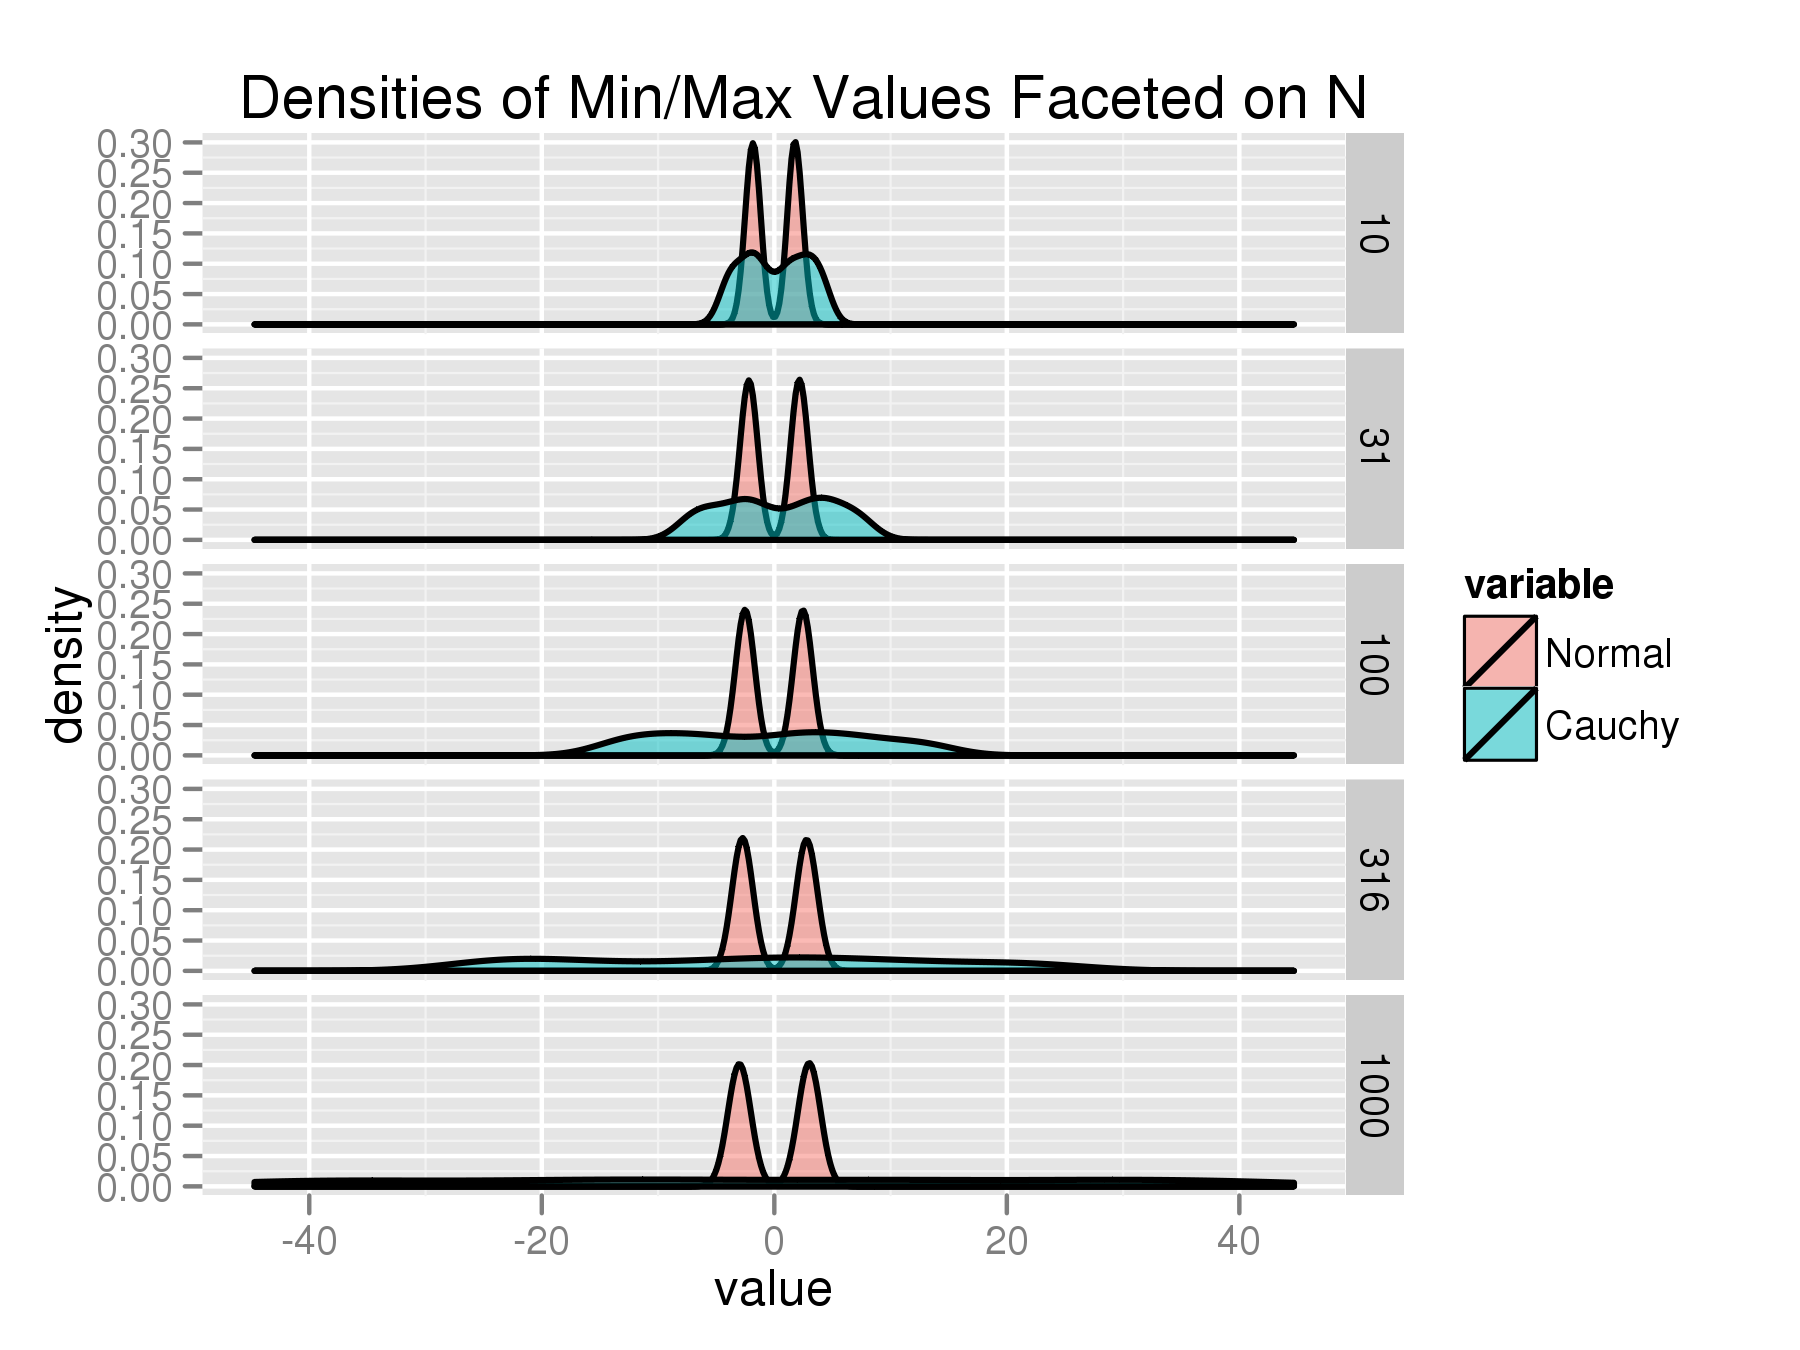
\includegraphics{./simulations/sim5.png}
\end{figure}

For $N=1000$, the Normal model typically has $u_{\Delta}$ values
around 6.  In contrast, the Cauchy model has $u_{\Delta}$ values
closer to 40.
\clearpage

Here, we plot the empirical Kolmogorov-Smirnov test statistic in the following three settings:
\begin{enumerate}
\item a standard Normal draw of size $N$ (repeated N times to get the empirical distribution)
\item the permutation $t$-statistic under Cauchy sampling (N permutations)
\item the permutation $t$-statistic under Normal sampling (N permutations)
\end{enumerate}
We also add the sum of the five unscaled, simulated bound terms ($200,000$ permutations) from the
previous section.

\begin{figure}[!ht]
  \centering
  % Created by tikzDevice version 0.6.2 on 2012-04-24 10:22:00
% !TEX encoding = UTF-8 Unicode
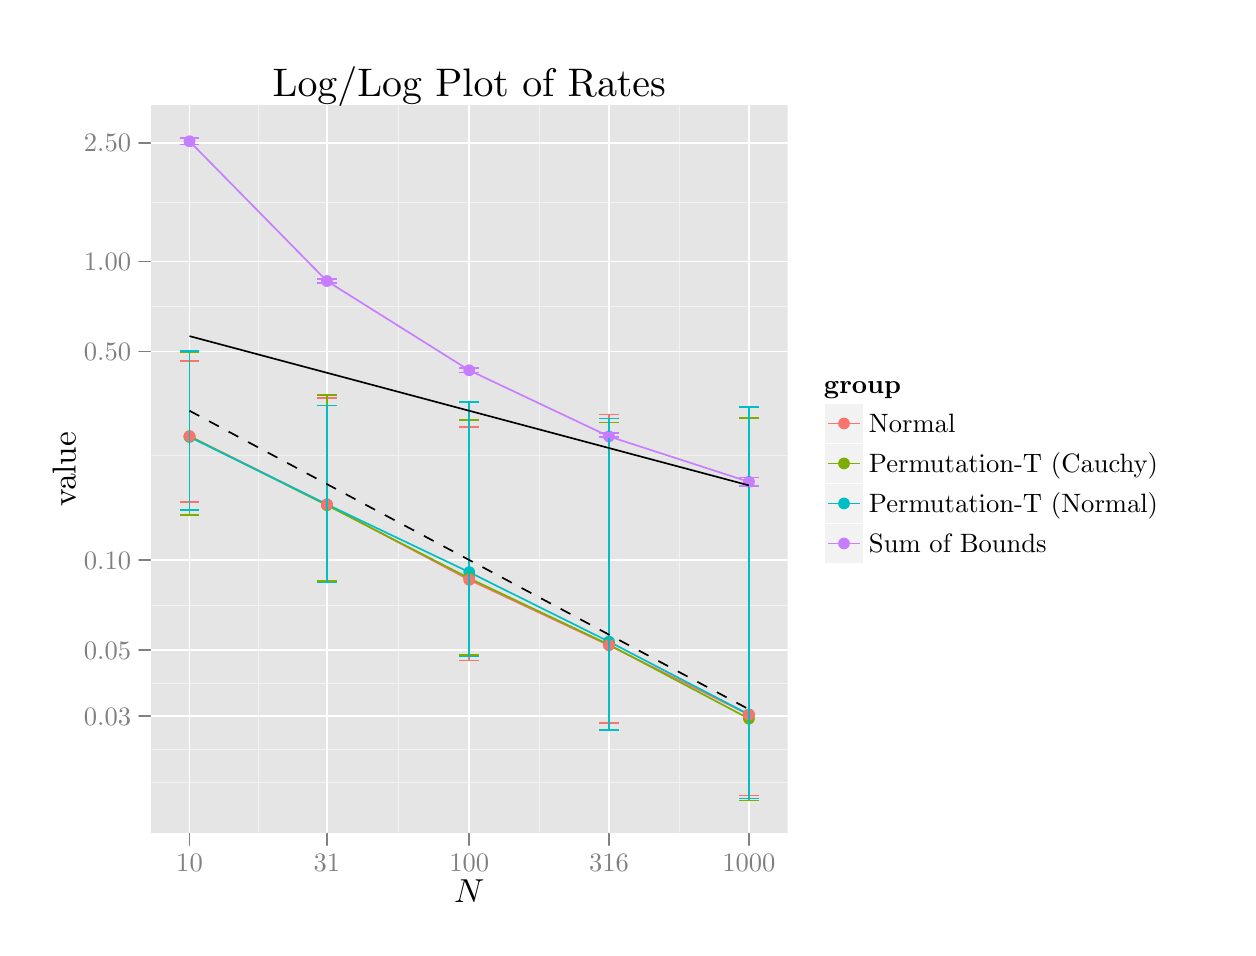
\begin{tikzpicture}[x=1pt,y=1pt]
\definecolor[named]{drawColor}{rgb}{0.00,0.00,0.00}
\definecolor[named]{fillColor}{rgb}{1.00,1.00,1.00}
\fill[color=fillColor,fill opacity=0.00,] (0,0) rectangle (433.62,325.21);
\begin{scope}
\path[clip] (  0.00,  0.00) rectangle (433.62,325.21);
\definecolor[named]{drawColor}{rgb}{0.41,0.16,0.58}
\end{scope}
\begin{scope}
\path[clip] (  0.00,  0.00) rectangle (433.62,325.21);
\definecolor[named]{drawColor}{rgb}{0.41,0.16,0.58}
\end{scope}
\begin{scope}
\path[clip] (  0.00,  0.00) rectangle (433.62,325.21);
\definecolor[named]{drawColor}{rgb}{0.41,0.16,0.58}
\end{scope}
\begin{scope}
\path[clip] (  0.00,  0.00) rectangle (433.62,325.21);
\definecolor[named]{drawColor}{rgb}{0.41,0.16,0.58}
\end{scope}
\begin{scope}
\path[clip] (  0.00,  0.00) rectangle (433.62,325.21);
\definecolor[named]{drawColor}{rgb}{0.41,0.16,0.58}
\end{scope}
\begin{scope}
\path[clip] (  0.00,  0.00) rectangle (433.62,325.21);
\definecolor[named]{drawColor}{rgb}{0.41,0.16,0.58}
\end{scope}
\begin{scope}
\path[clip] (  0.00,  0.00) rectangle (433.62,325.21);
\definecolor[named]{drawColor}{rgb}{0.41,0.16,0.58}
\end{scope}
\begin{scope}
\path[clip] (  0.00,  0.00) rectangle (433.62,325.21);
\definecolor[named]{drawColor}{rgb}{0.41,0.16,0.58}
\end{scope}
\begin{scope}
\path[clip] (  0.00,  0.00) rectangle (433.62,325.21);
\definecolor[named]{drawColor}{rgb}{0.41,0.16,0.58}
\end{scope}
\begin{scope}
\path[clip] (  0.00,  0.00) rectangle (433.62,325.21);
\definecolor[named]{drawColor}{rgb}{0.41,0.16,0.58}
\end{scope}
\begin{scope}
\path[clip] (  0.00,  0.00) rectangle (433.62,325.21);
\definecolor[named]{drawColor}{rgb}{0.41,0.16,0.58}
\end{scope}
\begin{scope}
\path[clip] (  0.00,  0.00) rectangle (433.62,325.21);
\definecolor[named]{drawColor}{rgb}{0.41,0.16,0.58}
\end{scope}
\begin{scope}
\path[clip] ( 44.49, 34.03) rectangle (274.61,297.23);
\definecolor[named]{drawColor}{rgb}{0.41,0.16,0.58}
\end{scope}
\begin{scope}
\path[clip] (  0.00,  0.00) rectangle (433.62,325.21);
\definecolor[named]{drawColor}{rgb}{0.41,0.16,0.58}
\end{scope}
\begin{scope}
\path[clip] (  0.00,  0.00) rectangle (433.62,325.21);
\definecolor[named]{drawColor}{rgb}{0.41,0.16,0.58}
\end{scope}
\begin{scope}
\path[clip] (  0.00,  0.00) rectangle (433.62,325.21);
\definecolor[named]{drawColor}{rgb}{0.41,0.16,0.58}
\end{scope}
\begin{scope}
\path[clip] (  0.00,  0.00) rectangle (433.62,325.21);
\definecolor[named]{drawColor}{rgb}{0.41,0.16,0.58}
\end{scope}
\begin{scope}
\path[clip] (  0.00,  0.00) rectangle (433.62,325.21);
\definecolor[named]{drawColor}{rgb}{0.41,0.16,0.58}
\end{scope}
\begin{scope}
\path[clip] (  0.00,  0.00) rectangle (433.62,325.21);
\definecolor[named]{drawColor}{rgb}{0.41,0.16,0.58}
\end{scope}
\begin{scope}
\path[clip] (  0.00,  0.00) rectangle (433.62,325.21);
\definecolor[named]{drawColor}{rgb}{0.41,0.16,0.58}
\end{scope}
\begin{scope}
\path[clip] (  0.00,  0.00) rectangle (433.62,325.21);
\definecolor[named]{drawColor}{rgb}{0.41,0.16,0.58}
\end{scope}
\begin{scope}
\path[clip] (  0.00,  0.00) rectangle (433.62,325.21);
\definecolor[named]{drawColor}{rgb}{0.41,0.16,0.58}
\end{scope}
\begin{scope}
\path[clip] (  0.00,  0.00) rectangle (433.62,325.21);
\definecolor[named]{drawColor}{rgb}{0.41,0.16,0.58}
\end{scope}
\begin{scope}
\path[clip] (  0.00,  0.00) rectangle (433.62,325.21);
\definecolor[named]{drawColor}{rgb}{0.41,0.16,0.58}
\end{scope}
\begin{scope}
\path[clip] (  0.00,  0.00) rectangle (433.62,325.21);
\definecolor[named]{drawColor}{rgb}{0.41,0.16,0.58}
\definecolor[named]{fillColor}{rgb}{1.00,1.00,1.00}

\draw[fill=fillColor,draw opacity=0.00,] (  0.00,  0.00) rectangle (433.62,325.21);
\end{scope}
\begin{scope}
\path[clip] (  0.00,  0.00) rectangle (433.62,325.21);
\definecolor[named]{drawColor}{rgb}{0.41,0.16,0.58}
\end{scope}
\begin{scope}
\path[clip] (  0.00,  0.00) rectangle (433.62,325.21);
\definecolor[named]{drawColor}{rgb}{0.41,0.16,0.58}
\definecolor[named]{drawColor}{rgb}{0.50,0.50,0.50}

\node[color=drawColor,anchor=base east,inner sep=0pt, outer sep=0pt, scale=  0.96] at ( 37.37, 73.13) {0.03};

\node[color=drawColor,anchor=base east,inner sep=0pt, outer sep=0pt, scale=  0.96] at ( 37.37, 97.07) {0.05};

\node[color=drawColor,anchor=base east,inner sep=0pt, outer sep=0pt, scale=  0.96] at ( 37.37,129.54) {0.10};

\node[color=drawColor,anchor=base east,inner sep=0pt, outer sep=0pt, scale=  0.96] at ( 37.37,204.94) {0.50};

\node[color=drawColor,anchor=base east,inner sep=0pt, outer sep=0pt, scale=  0.96] at ( 37.37,237.42) {1.00};

\node[color=drawColor,anchor=base east,inner sep=0pt, outer sep=0pt, scale=  0.96] at ( 37.37,280.34) {2.50};
\end{scope}
\begin{scope}
\path[clip] (  0.00,  0.00) rectangle (433.62,325.21);
\definecolor[named]{drawColor}{rgb}{0.41,0.16,0.58}
\definecolor[named]{drawColor}{rgb}{0.50,0.50,0.50}

\draw[color=drawColor,line width= 0.6pt,line cap=round,line join=round,fill opacity=0.00,] ( 40.22, 76.44) -- ( 44.49, 76.44);

\draw[color=drawColor,line width= 0.6pt,line cap=round,line join=round,fill opacity=0.00,] ( 40.22,100.37) -- ( 44.49,100.37);

\draw[color=drawColor,line width= 0.6pt,line cap=round,line join=round,fill opacity=0.00,] ( 40.22,132.85) -- ( 44.49,132.85);

\draw[color=drawColor,line width= 0.6pt,line cap=round,line join=round,fill opacity=0.00,] ( 40.22,208.25) -- ( 44.49,208.25);

\draw[color=drawColor,line width= 0.6pt,line cap=round,line join=round,fill opacity=0.00,] ( 40.22,240.72) -- ( 44.49,240.72);

\draw[color=drawColor,line width= 0.6pt,line cap=round,line join=round,fill opacity=0.00,] ( 40.22,283.65) -- ( 44.49,283.65);
\end{scope}
\begin{scope}
\path[clip] (  0.00,  0.00) rectangle (433.62,325.21);
\definecolor[named]{drawColor}{rgb}{0.41,0.16,0.58}
\end{scope}
\begin{scope}
\path[clip] (  0.00,  0.00) rectangle (433.62,325.21);
\definecolor[named]{drawColor}{rgb}{0.41,0.16,0.58}
\end{scope}
\begin{scope}
\path[clip] (  0.00,  0.00) rectangle (433.62,325.21);
\definecolor[named]{drawColor}{rgb}{0.41,0.16,0.58}
\end{scope}
\begin{scope}
\path[clip] (  0.00,  0.00) rectangle (433.62,325.21);
\definecolor[named]{drawColor}{rgb}{0.41,0.16,0.58}
\end{scope}
\begin{scope}
\path[clip] (  0.00,  0.00) rectangle (433.62,325.21);
\definecolor[named]{drawColor}{rgb}{0.41,0.16,0.58}
\end{scope}
\begin{scope}
\path[clip] ( 44.49, 34.03) rectangle (274.61,297.23);
\definecolor[named]{drawColor}{rgb}{0.41,0.16,0.58}
\definecolor[named]{fillColor}{rgb}{0.90,0.90,0.90}

\draw[fill=fillColor,draw opacity=0.00,] ( 44.49, 34.03) rectangle (274.61,297.23);
\definecolor[named]{drawColor}{rgb}{0.95,0.95,0.95}

\draw[color=drawColor,line width= 0.3pt,line cap=round,line join=round,fill opacity=0.00,] ( 44.49, 52.51) --
	(274.61, 52.51);

\draw[color=drawColor,line width= 0.3pt,line cap=round,line join=round,fill opacity=0.00,] ( 44.49, 64.47) --
	(274.61, 64.47);

\draw[color=drawColor,line width= 0.3pt,line cap=round,line join=round,fill opacity=0.00,] ( 44.49, 88.41) --
	(274.61, 88.41);

\draw[color=drawColor,line width= 0.3pt,line cap=round,line join=round,fill opacity=0.00,] ( 44.49,116.61) --
	(274.61,116.61);

\draw[color=drawColor,line width= 0.3pt,line cap=round,line join=round,fill opacity=0.00,] ( 44.49,170.55) --
	(274.61,170.55);

\draw[color=drawColor,line width= 0.3pt,line cap=round,line join=round,fill opacity=0.00,] ( 44.49,224.49) --
	(274.61,224.49);

\draw[color=drawColor,line width= 0.3pt,line cap=round,line join=round,fill opacity=0.00,] ( 44.49,262.19) --
	(274.61,262.19);

\draw[color=drawColor,line width= 0.3pt,line cap=round,line join=round,fill opacity=0.00,] ( 83.31, 34.03) --
	( 83.31,297.23);

\draw[color=drawColor,line width= 0.3pt,line cap=round,line join=round,fill opacity=0.00,] (133.85, 34.03) --
	(133.85,297.23);

\draw[color=drawColor,line width= 0.3pt,line cap=round,line join=round,fill opacity=0.00,] (184.80, 34.03) --
	(184.80,297.23);

\draw[color=drawColor,line width= 0.3pt,line cap=round,line join=round,fill opacity=0.00,] (235.33, 34.03) --
	(235.33,297.23);
\definecolor[named]{drawColor}{rgb}{1.00,1.00,1.00}

\draw[color=drawColor,line width= 0.6pt,line cap=round,line join=round,fill opacity=0.00,] ( 44.49, 76.44) --
	(274.61, 76.44);

\draw[color=drawColor,line width= 0.6pt,line cap=round,line join=round,fill opacity=0.00,] ( 44.49,100.37) --
	(274.61,100.37);

\draw[color=drawColor,line width= 0.6pt,line cap=round,line join=round,fill opacity=0.00,] ( 44.49,132.85) --
	(274.61,132.85);

\draw[color=drawColor,line width= 0.6pt,line cap=round,line join=round,fill opacity=0.00,] ( 44.49,208.25) --
	(274.61,208.25);

\draw[color=drawColor,line width= 0.6pt,line cap=round,line join=round,fill opacity=0.00,] ( 44.49,240.72) --
	(274.61,240.72);

\draw[color=drawColor,line width= 0.6pt,line cap=round,line join=round,fill opacity=0.00,] ( 44.49,283.65) --
	(274.61,283.65);

\draw[color=drawColor,line width= 0.6pt,line cap=round,line join=round,fill opacity=0.00,] ( 58.48, 34.03) --
	( 58.48,297.23);

\draw[color=drawColor,line width= 0.6pt,line cap=round,line join=round,fill opacity=0.00,] (108.14, 34.03) --
	(108.14,297.23);

\draw[color=drawColor,line width= 0.6pt,line cap=round,line join=round,fill opacity=0.00,] (159.55, 34.03) --
	(159.55,297.23);

\draw[color=drawColor,line width= 0.6pt,line cap=round,line join=round,fill opacity=0.00,] (210.05, 34.03) --
	(210.05,297.23);

\draw[color=drawColor,line width= 0.6pt,line cap=round,line join=round,fill opacity=0.00,] (260.62, 34.03) --
	(260.62,297.23);
\definecolor[named]{drawColor}{rgb}{0.97,0.46,0.43}

\draw[color=drawColor,line width= 0.6pt,line join=round,fill opacity=0.00,] ( 58.48,177.61) --
	(108.14,152.89) --
	(159.55,125.69) --
	(210.05,102.01) --
	(260.62, 76.96);
\definecolor[named]{drawColor}{rgb}{0.49,0.68,0.00}

\draw[color=drawColor,line width= 0.6pt,line join=round,fill opacity=0.00,] ( 58.48,177.55) --
	(108.14,152.64) --
	(159.55,126.25) --
	(210.05,102.26) --
	(260.62, 75.52);
\definecolor[named]{drawColor}{rgb}{0.00,0.75,0.77}

\draw[color=drawColor,line width= 0.6pt,line join=round,fill opacity=0.00,] ( 58.48,177.31) --
	(108.14,152.96) --
	(159.55,128.45) --
	(210.05,103.35) --
	(260.62, 77.05);
\definecolor[named]{drawColor}{rgb}{0.78,0.49,1.00}

\draw[color=drawColor,line width= 0.6pt,line join=round,fill opacity=0.00,] ( 58.48,284.15) --
	(108.14,233.65) --
	(159.55,201.40) --
	(210.05,177.51) --
	(260.62,161.10);
\definecolor[named]{fillColor}{rgb}{0.00,0.75,0.77}

\draw[fill=fillColor,draw opacity=0.00,] ( 58.48,177.31) circle (  2.13);
\definecolor[named]{fillColor}{rgb}{0.49,0.68,0.00}

\draw[fill=fillColor,draw opacity=0.00,] ( 58.48,177.55) circle (  2.13);
\definecolor[named]{fillColor}{rgb}{0.97,0.46,0.43}

\draw[fill=fillColor,draw opacity=0.00,] ( 58.48,177.61) circle (  2.13);
\definecolor[named]{fillColor}{rgb}{0.00,0.75,0.77}

\draw[fill=fillColor,draw opacity=0.00,] (108.14,152.96) circle (  2.13);
\definecolor[named]{fillColor}{rgb}{0.49,0.68,0.00}

\draw[fill=fillColor,draw opacity=0.00,] (108.14,152.64) circle (  2.13);
\definecolor[named]{fillColor}{rgb}{0.97,0.46,0.43}

\draw[fill=fillColor,draw opacity=0.00,] (108.14,152.89) circle (  2.13);
\definecolor[named]{fillColor}{rgb}{0.00,0.75,0.77}

\draw[fill=fillColor,draw opacity=0.00,] (159.55,128.45) circle (  2.13);
\definecolor[named]{fillColor}{rgb}{0.49,0.68,0.00}

\draw[fill=fillColor,draw opacity=0.00,] (159.55,126.25) circle (  2.13);
\definecolor[named]{fillColor}{rgb}{0.97,0.46,0.43}

\draw[fill=fillColor,draw opacity=0.00,] (159.55,125.69) circle (  2.13);
\definecolor[named]{fillColor}{rgb}{0.00,0.75,0.77}

\draw[fill=fillColor,draw opacity=0.00,] (210.05,103.35) circle (  2.13);
\definecolor[named]{fillColor}{rgb}{0.49,0.68,0.00}

\draw[fill=fillColor,draw opacity=0.00,] (210.05,102.26) circle (  2.13);
\definecolor[named]{fillColor}{rgb}{0.97,0.46,0.43}

\draw[fill=fillColor,draw opacity=0.00,] (210.05,102.01) circle (  2.13);
\definecolor[named]{fillColor}{rgb}{0.00,0.75,0.77}

\draw[fill=fillColor,draw opacity=0.00,] (260.62, 77.05) circle (  2.13);
\definecolor[named]{fillColor}{rgb}{0.49,0.68,0.00}

\draw[fill=fillColor,draw opacity=0.00,] (260.62, 75.52) circle (  2.13);
\definecolor[named]{fillColor}{rgb}{0.97,0.46,0.43}

\draw[fill=fillColor,draw opacity=0.00,] (260.62, 76.96) circle (  2.13);
\definecolor[named]{fillColor}{rgb}{0.78,0.49,1.00}

\draw[fill=fillColor,draw opacity=0.00,] ( 58.48,284.15) circle (  2.13);

\draw[fill=fillColor,draw opacity=0.00,] (108.14,233.65) circle (  2.13);

\draw[fill=fillColor,draw opacity=0.00,] (159.55,201.40) circle (  2.13);

\draw[fill=fillColor,draw opacity=0.00,] (210.05,177.51) circle (  2.13);

\draw[fill=fillColor,draw opacity=0.00,] (260.62,161.10) circle (  2.13);
\definecolor[named]{drawColor}{rgb}{0.97,0.46,0.43}

\draw[color=drawColor,line width= 0.6pt,line join=round,fill opacity=0.00,] ( 54.95,204.74) --
	( 62.02,204.74);

\draw[color=drawColor,line width= 0.6pt,line join=round,fill opacity=0.00,] ( 58.48,204.74) --
	( 58.48,153.80);

\draw[color=drawColor,line width= 0.6pt,line join=round,fill opacity=0.00,] ( 54.95,153.80) --
	( 62.02,153.80);

\draw[color=drawColor,line width= 0.6pt,line join=round,fill opacity=0.00,] (104.61,191.45) --
	(111.68,191.45);

\draw[color=drawColor,line width= 0.6pt,line join=round,fill opacity=0.00,] (108.14,191.45) --
	(108.14,125.00);

\draw[color=drawColor,line width= 0.6pt,line join=round,fill opacity=0.00,] (104.61,125.00) --
	(111.68,125.00);

\draw[color=drawColor,line width= 0.6pt,line join=round,fill opacity=0.00,] (156.01,181.01) --
	(163.09,181.01);

\draw[color=drawColor,line width= 0.6pt,line join=round,fill opacity=0.00,] (159.55,181.01) --
	(159.55, 96.56);

\draw[color=drawColor,line width= 0.6pt,line join=round,fill opacity=0.00,] (156.01, 96.56) --
	(163.09, 96.56);

\draw[color=drawColor,line width= 0.6pt,line join=round,fill opacity=0.00,] (206.51,185.42) --
	(213.59,185.42);

\draw[color=drawColor,line width= 0.6pt,line join=round,fill opacity=0.00,] (210.05,185.42) --
	(210.05, 73.96);

\draw[color=drawColor,line width= 0.6pt,line join=round,fill opacity=0.00,] (206.51, 73.96) --
	(213.59, 73.96);

\draw[color=drawColor,line width= 0.6pt,line join=round,fill opacity=0.00,] (257.08,184.36) --
	(264.15,184.36);

\draw[color=drawColor,line width= 0.6pt,line join=round,fill opacity=0.00,] (260.62,184.36) --
	(260.62, 47.72);

\draw[color=drawColor,line width= 0.6pt,line join=round,fill opacity=0.00,] (257.08, 47.72) --
	(264.15, 47.72);
\definecolor[named]{drawColor}{rgb}{0.49,0.68,0.00}

\draw[color=drawColor,line width= 0.6pt,line join=round,fill opacity=0.00,] ( 54.95,207.80) --
	( 62.02,207.80);

\draw[color=drawColor,line width= 0.6pt,line join=round,fill opacity=0.00,] ( 58.48,207.80) --
	( 58.48,149.16);

\draw[color=drawColor,line width= 0.6pt,line join=round,fill opacity=0.00,] ( 54.95,149.16) --
	( 62.02,149.16);

\draw[color=drawColor,line width= 0.6pt,line join=round,fill opacity=0.00,] (104.61,192.36) --
	(111.68,192.36);

\draw[color=drawColor,line width= 0.6pt,line join=round,fill opacity=0.00,] (108.14,192.36) --
	(108.14,125.24);

\draw[color=drawColor,line width= 0.6pt,line join=round,fill opacity=0.00,] (104.61,125.24) --
	(111.68,125.24);

\draw[color=drawColor,line width= 0.6pt,line join=round,fill opacity=0.00,] (156.01,183.42) --
	(163.09,183.42);

\draw[color=drawColor,line width= 0.6pt,line join=round,fill opacity=0.00,] (159.55,183.42) --
	(159.55, 98.53);

\draw[color=drawColor,line width= 0.6pt,line join=round,fill opacity=0.00,] (156.01, 98.53) --
	(163.09, 98.53);

\draw[color=drawColor,line width= 0.6pt,line join=round,fill opacity=0.00,] (206.51,182.54) --
	(213.59,182.54);

\draw[color=drawColor,line width= 0.6pt,line join=round,fill opacity=0.00,] (210.05,182.54) --
	(210.05, 71.65);

\draw[color=drawColor,line width= 0.6pt,line join=round,fill opacity=0.00,] (206.51, 71.65) --
	(213.59, 71.65);

\draw[color=drawColor,line width= 0.6pt,line join=round,fill opacity=0.00,] (257.08,184.20) --
	(264.15,184.20);

\draw[color=drawColor,line width= 0.6pt,line join=round,fill opacity=0.00,] (260.62,184.20) --
	(260.62, 46.00);

\draw[color=drawColor,line width= 0.6pt,line join=round,fill opacity=0.00,] (257.08, 46.00) --
	(264.15, 46.00);
\definecolor[named]{drawColor}{rgb}{0.00,0.75,0.77}

\draw[color=drawColor,line width= 0.6pt,line join=round,fill opacity=0.00,] ( 54.95,208.27) --
	( 62.02,208.27);

\draw[color=drawColor,line width= 0.6pt,line join=round,fill opacity=0.00,] ( 58.48,208.27) --
	( 58.48,150.80);

\draw[color=drawColor,line width= 0.6pt,line join=round,fill opacity=0.00,] ( 54.95,150.80) --
	( 62.02,150.80);

\draw[color=drawColor,line width= 0.6pt,line join=round,fill opacity=0.00,] (104.61,188.64) --
	(111.68,188.64);

\draw[color=drawColor,line width= 0.6pt,line join=round,fill opacity=0.00,] (108.14,188.64) --
	(108.14,124.72);

\draw[color=drawColor,line width= 0.6pt,line join=round,fill opacity=0.00,] (104.61,124.72) --
	(111.68,124.72);

\draw[color=drawColor,line width= 0.6pt,line join=round,fill opacity=0.00,] (156.01,189.99) --
	(163.09,189.99);

\draw[color=drawColor,line width= 0.6pt,line join=round,fill opacity=0.00,] (159.55,189.99) --
	(159.55, 98.00);

\draw[color=drawColor,line width= 0.6pt,line join=round,fill opacity=0.00,] (156.01, 98.00) --
	(163.09, 98.00);

\draw[color=drawColor,line width= 0.6pt,line join=round,fill opacity=0.00,] (206.51,183.95) --
	(213.59,183.95);

\draw[color=drawColor,line width= 0.6pt,line join=round,fill opacity=0.00,] (210.05,183.95) --
	(210.05, 71.48);

\draw[color=drawColor,line width= 0.6pt,line join=round,fill opacity=0.00,] (206.51, 71.48) --
	(213.59, 71.48);

\draw[color=drawColor,line width= 0.6pt,line join=round,fill opacity=0.00,] (257.08,188.23) --
	(264.15,188.23);

\draw[color=drawColor,line width= 0.6pt,line join=round,fill opacity=0.00,] (260.62,188.23) --
	(260.62, 46.65);

\draw[color=drawColor,line width= 0.6pt,line join=round,fill opacity=0.00,] (257.08, 46.65) --
	(264.15, 46.65);
\definecolor[named]{drawColor}{rgb}{0.78,0.49,1.00}

\draw[color=drawColor,line width= 0.6pt,line join=round,fill opacity=0.00,] ( 54.95,285.27) --
	( 62.02,285.27);

\draw[color=drawColor,line width= 0.6pt,line join=round,fill opacity=0.00,] ( 58.48,285.27) --
	( 58.48,283.02);

\draw[color=drawColor,line width= 0.6pt,line join=round,fill opacity=0.00,] ( 54.95,283.02) --
	( 62.02,283.02);

\draw[color=drawColor,line width= 0.6pt,line join=round,fill opacity=0.00,] (104.61,234.28) --
	(111.68,234.28);

\draw[color=drawColor,line width= 0.6pt,line join=round,fill opacity=0.00,] (108.14,234.28) --
	(108.14,233.01);

\draw[color=drawColor,line width= 0.6pt,line join=round,fill opacity=0.00,] (104.61,233.01) --
	(111.68,233.01);

\draw[color=drawColor,line width= 0.6pt,line join=round,fill opacity=0.00,] (156.01,202.24) --
	(163.09,202.24);

\draw[color=drawColor,line width= 0.6pt,line join=round,fill opacity=0.00,] (159.55,202.24) --
	(159.55,200.59);

\draw[color=drawColor,line width= 0.6pt,line join=round,fill opacity=0.00,] (156.01,200.59) --
	(163.09,200.59);

\draw[color=drawColor,line width= 0.6pt,line join=round,fill opacity=0.00,] (206.51,178.78) --
	(213.59,178.78);

\draw[color=drawColor,line width= 0.6pt,line join=round,fill opacity=0.00,] (210.05,178.78) --
	(210.05,177.26);

\draw[color=drawColor,line width= 0.6pt,line join=round,fill opacity=0.00,] (206.51,177.26) --
	(213.59,177.26);

\draw[color=drawColor,line width= 0.6pt,line join=round,fill opacity=0.00,] (257.08,162.61) --
	(264.15,162.61);

\draw[color=drawColor,line width= 0.6pt,line join=round,fill opacity=0.00,] (260.62,162.61) --
	(260.62,159.55);

\draw[color=drawColor,line width= 0.6pt,line join=round,fill opacity=0.00,] (257.08,159.55) --
	(264.15,159.55);
\definecolor[named]{drawColor}{rgb}{0.00,0.00,0.00}

\draw[color=drawColor,line width= 0.6pt,dash pattern=on 4pt off 4pt ,line join=round,fill opacity=0.00,] ( 58.48,186.78) --
	( 58.48,186.78) --
	( 58.48,186.78) --
	( 58.48,186.78) --
	(108.14,160.28) --
	(108.14,160.28) --
	(108.14,160.28) --
	(108.14,160.28) --
	(159.55,132.85) --
	(159.55,132.85) --
	(159.55,132.85) --
	(159.55,132.85) --
	(210.05,105.89) --
	(210.05,105.89) --
	(210.05,105.89) --
	(210.05,105.89) --
	(260.62, 78.91) --
	(260.62, 78.91) --
	(260.62, 78.91) --
	(260.62, 78.91);

\draw[color=drawColor,line width= 0.6pt,line join=round,fill opacity=0.00,] ( 58.48,213.75) --
	( 58.48,213.75) --
	( 58.48,213.75) --
	( 58.48,213.75) --
	(108.14,200.50) --
	(108.14,200.50) --
	(108.14,200.50) --
	(108.14,200.50) --
	(159.55,186.78) --
	(159.55,186.78) --
	(159.55,186.78) --
	(159.55,186.78) --
	(210.05,173.31) --
	(210.05,173.31) --
	(210.05,173.31) --
	(210.05,173.31) --
	(260.62,159.82) --
	(260.62,159.82) --
	(260.62,159.82) --
	(260.62,159.82);
\end{scope}
\begin{scope}
\path[clip] (  0.00,  0.00) rectangle (433.62,325.21);
\definecolor[named]{drawColor}{rgb}{0.41,0.16,0.58}
\end{scope}
\begin{scope}
\path[clip] (  0.00,  0.00) rectangle (433.62,325.21);
\definecolor[named]{drawColor}{rgb}{0.41,0.16,0.58}
\definecolor[named]{drawColor}{rgb}{0.50,0.50,0.50}

\node[color=drawColor,anchor=base,inner sep=0pt, outer sep=0pt, scale=  0.96] at ( 58.48, 20.31) {10};

\node[color=drawColor,anchor=base,inner sep=0pt, outer sep=0pt, scale=  0.96] at (108.14, 20.31) {31};

\node[color=drawColor,anchor=base,inner sep=0pt, outer sep=0pt, scale=  0.96] at (159.55, 20.31) {100};

\node[color=drawColor,anchor=base,inner sep=0pt, outer sep=0pt, scale=  0.96] at (210.05, 20.31) {316};

\node[color=drawColor,anchor=base,inner sep=0pt, outer sep=0pt, scale=  0.96] at (260.62, 20.31) {1000};
\end{scope}
\begin{scope}
\path[clip] (  0.00,  0.00) rectangle (433.62,325.21);
\definecolor[named]{drawColor}{rgb}{0.41,0.16,0.58}
\definecolor[named]{drawColor}{rgb}{0.50,0.50,0.50}

\draw[color=drawColor,line width= 0.6pt,line cap=round,line join=round,fill opacity=0.00,] ( 58.48, 29.77) -- ( 58.48, 34.03);

\draw[color=drawColor,line width= 0.6pt,line cap=round,line join=round,fill opacity=0.00,] (108.14, 29.77) -- (108.14, 34.03);

\draw[color=drawColor,line width= 0.6pt,line cap=round,line join=round,fill opacity=0.00,] (159.55, 29.77) -- (159.55, 34.03);

\draw[color=drawColor,line width= 0.6pt,line cap=round,line join=round,fill opacity=0.00,] (210.05, 29.77) -- (210.05, 34.03);

\draw[color=drawColor,line width= 0.6pt,line cap=round,line join=round,fill opacity=0.00,] (260.62, 29.77) -- (260.62, 34.03);
\end{scope}
\begin{scope}
\path[clip] (  0.00,  0.00) rectangle (433.62,325.21);
\definecolor[named]{drawColor}{rgb}{0.41,0.16,0.58}
\end{scope}
\begin{scope}
\path[clip] (  0.00,  0.00) rectangle (433.62,325.21);
\definecolor[named]{drawColor}{rgb}{0.41,0.16,0.58}
\end{scope}
\begin{scope}
\path[clip] (  0.00,  0.00) rectangle (433.62,325.21);
\definecolor[named]{drawColor}{rgb}{0.41,0.16,0.58}
\end{scope}
\begin{scope}
\path[clip] (  0.00,  0.00) rectangle (433.62,325.21);
\definecolor[named]{drawColor}{rgb}{0.41,0.16,0.58}
\definecolor[named]{drawColor}{rgb}{0.00,0.00,0.00}

\node[color=drawColor,anchor=base,inner sep=0pt, outer sep=0pt, scale=  1.44] at (159.55,300.24) {Log/Log Plot of Rates};
\end{scope}
\begin{scope}
\path[clip] (  0.00,  0.00) rectangle (433.62,325.21);
\definecolor[named]{drawColor}{rgb}{0.41,0.16,0.58}
\end{scope}
\begin{scope}
\path[clip] (  0.00,  0.00) rectangle (433.62,325.21);
\definecolor[named]{drawColor}{rgb}{0.41,0.16,0.58}
\definecolor[named]{drawColor}{rgb}{0.00,0.00,0.00}

\node[color=drawColor,anchor=base,inner sep=0pt, outer sep=0pt, scale=  1.20] at (159.55,  9.03) {$N$};
\end{scope}
\begin{scope}
\path[clip] (  0.00,  0.00) rectangle (433.62,325.21);
\definecolor[named]{drawColor}{rgb}{0.41,0.16,0.58}
\end{scope}
\begin{scope}
\path[clip] (  0.00,  0.00) rectangle (433.62,325.21);
\definecolor[named]{drawColor}{rgb}{0.41,0.16,0.58}
\definecolor[named]{drawColor}{rgb}{0.00,0.00,0.00}

\node[rotate= 90.00,color=drawColor,anchor=base,inner sep=0pt, outer sep=0pt, scale=  1.20] at ( 17.30,165.63) {value};
\end{scope}
\begin{scope}
\path[clip] (  0.00,  0.00) rectangle (433.62,325.21);
\definecolor[named]{drawColor}{rgb}{0.41,0.16,0.58}
\end{scope}
\begin{scope}
\path[clip] (  0.00,  0.00) rectangle (433.62,325.21);
\definecolor[named]{drawColor}{rgb}{0.41,0.16,0.58}
\end{scope}
\begin{scope}
\path[clip] (  0.00,  0.00) rectangle (433.62,325.21);
\definecolor[named]{drawColor}{rgb}{0.41,0.16,0.58}
\end{scope}
\begin{scope}
\path[clip] (  0.00,  0.00) rectangle (433.62,325.21);
\definecolor[named]{drawColor}{rgb}{0.41,0.16,0.58}
\end{scope}
\begin{scope}
\path[clip] (  0.00,  0.00) rectangle (433.62,325.21);
\definecolor[named]{drawColor}{rgb}{0.41,0.16,0.58}
\end{scope}
\begin{scope}
\path[clip] (  0.00,  0.00) rectangle (433.62,325.21);
\definecolor[named]{drawColor}{rgb}{0.41,0.16,0.58}
\end{scope}
\begin{scope}
\path[clip] (  0.00,  0.00) rectangle (433.62,325.21);
\definecolor[named]{drawColor}{rgb}{0.41,0.16,0.58}
\end{scope}
\begin{scope}
\path[clip] (  0.00,  0.00) rectangle (433.62,325.21);
\definecolor[named]{drawColor}{rgb}{0.41,0.16,0.58}
\end{scope}
\begin{scope}
\path[clip] (  0.00,  0.00) rectangle (433.62,325.21);
\definecolor[named]{drawColor}{rgb}{0.41,0.16,0.58}
\end{scope}
\begin{scope}
\path[clip] (  0.00,  0.00) rectangle (433.62,325.21);
\definecolor[named]{drawColor}{rgb}{0.41,0.16,0.58}
\end{scope}
\begin{scope}
\path[clip] (  0.00,  0.00) rectangle (433.62,325.21);
\definecolor[named]{drawColor}{rgb}{0.41,0.16,0.58}
\end{scope}
\begin{scope}
\path[clip] (  0.00,  0.00) rectangle (433.62,325.21);
\definecolor[named]{drawColor}{rgb}{0.41,0.16,0.58}
\end{scope}
\begin{scope}
\path[clip] (  0.00,  0.00) rectangle (433.62,325.21);
\definecolor[named]{drawColor}{rgb}{0.41,0.16,0.58}
\end{scope}
\begin{scope}
\path[clip] (  0.00,  0.00) rectangle (433.62,325.21);
\definecolor[named]{drawColor}{rgb}{0.41,0.16,0.58}
\end{scope}
\begin{scope}
\path[clip] (  0.00,  0.00) rectangle (433.62,325.21);
\definecolor[named]{drawColor}{rgb}{0.41,0.16,0.58}
\end{scope}
\begin{scope}
\path[clip] (  0.00,  0.00) rectangle (433.62,325.21);
\definecolor[named]{drawColor}{rgb}{0.41,0.16,0.58}
\end{scope}
\begin{scope}
\path[clip] (  0.00,  0.00) rectangle (433.62,325.21);
\definecolor[named]{drawColor}{rgb}{0.41,0.16,0.58}
\end{scope}
\begin{scope}
\path[clip] (  0.00,  0.00) rectangle (433.62,325.21);
\definecolor[named]{drawColor}{rgb}{0.41,0.16,0.58}
\end{scope}
\begin{scope}
\path[clip] (  0.00,  0.00) rectangle (433.62,325.21);
\definecolor[named]{drawColor}{rgb}{0.41,0.16,0.58}
\end{scope}
\begin{scope}
\path[clip] (  0.00,  0.00) rectangle (433.62,325.21);
\definecolor[named]{drawColor}{rgb}{0.41,0.16,0.58}
\end{scope}
\begin{scope}
\path[clip] (  0.00,  0.00) rectangle (433.62,325.21);
\definecolor[named]{drawColor}{rgb}{0.41,0.16,0.58}
\end{scope}
\begin{scope}
\path[clip] (  0.00,  0.00) rectangle (433.62,325.21);
\definecolor[named]{drawColor}{rgb}{0.41,0.16,0.58}
\end{scope}
\begin{scope}
\path[clip] (  0.00,  0.00) rectangle (433.62,325.21);
\definecolor[named]{drawColor}{rgb}{0.41,0.16,0.58}
\end{scope}
\begin{scope}
\path[clip] (  0.00,  0.00) rectangle (433.62,325.21);
\definecolor[named]{drawColor}{rgb}{0.41,0.16,0.58}
\end{scope}
\begin{scope}
\path[clip] (  0.00,  0.00) rectangle (433.62,325.21);
\definecolor[named]{drawColor}{rgb}{0.41,0.16,0.58}
\definecolor[named]{drawColor}{rgb}{1.00,1.00,1.00}

\draw[color=drawColor,line width= 0.6pt,line cap=round,line join=round,fill opacity=0.00,] (283.48,127.34) rectangle (412.71,203.93);
\end{scope}
\begin{scope}
\path[clip] (  0.00,  0.00) rectangle (433.62,325.21);
\definecolor[named]{drawColor}{rgb}{0.41,0.16,0.58}
\definecolor[named]{drawColor}{rgb}{0.00,0.00,0.00}

\node[color=drawColor,anchor=base west,inner sep=0pt, outer sep=0pt, scale=  0.96] at (287.75,193.03) {\bfseries group};
\end{scope}
\begin{scope}
\path[clip] (  0.00,  0.00) rectangle (433.62,325.21);
\definecolor[named]{drawColor}{rgb}{0.41,0.16,0.58}
\definecolor[named]{drawColor}{rgb}{1.00,1.00,1.00}
\definecolor[named]{fillColor}{rgb}{0.95,0.95,0.95}

\draw[color=drawColor,line width= 0.6pt,line cap=round,line join=round,fill=fillColor,] (287.75,174.97) rectangle (302.20,189.42);
\end{scope}
\begin{scope}
\path[clip] (  0.00,  0.00) rectangle (433.62,325.21);
\definecolor[named]{drawColor}{rgb}{0.41,0.16,0.58}
\definecolor[named]{drawColor}{rgb}{0.97,0.46,0.43}

\draw[color=drawColor,line width= 0.6pt,line join=round,fill opacity=0.00,] (289.20,182.19) -- (300.76,182.19);
\end{scope}
\begin{scope}
\path[clip] (  0.00,  0.00) rectangle (433.62,325.21);
\definecolor[named]{drawColor}{rgb}{0.41,0.16,0.58}
\definecolor[named]{fillColor}{rgb}{0.97,0.46,0.43}

\draw[fill=fillColor,draw opacity=0.00,] (294.98,182.19) circle (  2.13);
\end{scope}
\begin{scope}
\path[clip] (  0.00,  0.00) rectangle (433.62,325.21);
\definecolor[named]{drawColor}{rgb}{0.41,0.16,0.58}
\definecolor[named]{drawColor}{rgb}{0.97,0.46,0.43}

\draw[color=drawColor,line width= 0.6pt,line join=round,fill opacity=0.00,] (289.20,182.19) -- (300.76,182.19);
\end{scope}
\begin{scope}
\path[clip] (  0.00,  0.00) rectangle (433.62,325.21);
\definecolor[named]{drawColor}{rgb}{0.41,0.16,0.58}
\definecolor[named]{drawColor}{rgb}{1.00,1.00,1.00}
\definecolor[named]{fillColor}{rgb}{0.95,0.95,0.95}

\draw[color=drawColor,line width= 0.6pt,line cap=round,line join=round,fill=fillColor,] (287.75,160.51) rectangle (302.20,174.97);
\end{scope}
\begin{scope}
\path[clip] (  0.00,  0.00) rectangle (433.62,325.21);
\definecolor[named]{drawColor}{rgb}{0.41,0.16,0.58}
\definecolor[named]{drawColor}{rgb}{0.49,0.68,0.00}

\draw[color=drawColor,line width= 0.6pt,line join=round,fill opacity=0.00,] (289.20,167.74) -- (300.76,167.74);
\end{scope}
\begin{scope}
\path[clip] (  0.00,  0.00) rectangle (433.62,325.21);
\definecolor[named]{drawColor}{rgb}{0.41,0.16,0.58}
\definecolor[named]{fillColor}{rgb}{0.49,0.68,0.00}

\draw[fill=fillColor,draw opacity=0.00,] (294.98,167.74) circle (  2.13);
\end{scope}
\begin{scope}
\path[clip] (  0.00,  0.00) rectangle (433.62,325.21);
\definecolor[named]{drawColor}{rgb}{0.41,0.16,0.58}
\definecolor[named]{drawColor}{rgb}{0.49,0.68,0.00}

\draw[color=drawColor,line width= 0.6pt,line join=round,fill opacity=0.00,] (289.20,167.74) -- (300.76,167.74);
\end{scope}
\begin{scope}
\path[clip] (  0.00,  0.00) rectangle (433.62,325.21);
\definecolor[named]{drawColor}{rgb}{0.41,0.16,0.58}
\definecolor[named]{drawColor}{rgb}{1.00,1.00,1.00}
\definecolor[named]{fillColor}{rgb}{0.95,0.95,0.95}

\draw[color=drawColor,line width= 0.6pt,line cap=round,line join=round,fill=fillColor,] (287.75,146.06) rectangle (302.20,160.51);
\end{scope}
\begin{scope}
\path[clip] (  0.00,  0.00) rectangle (433.62,325.21);
\definecolor[named]{drawColor}{rgb}{0.41,0.16,0.58}
\definecolor[named]{drawColor}{rgb}{0.00,0.75,0.77}

\draw[color=drawColor,line width= 0.6pt,line join=round,fill opacity=0.00,] (289.20,153.29) -- (300.76,153.29);
\end{scope}
\begin{scope}
\path[clip] (  0.00,  0.00) rectangle (433.62,325.21);
\definecolor[named]{drawColor}{rgb}{0.41,0.16,0.58}
\definecolor[named]{fillColor}{rgb}{0.00,0.75,0.77}

\draw[fill=fillColor,draw opacity=0.00,] (294.98,153.29) circle (  2.13);
\end{scope}
\begin{scope}
\path[clip] (  0.00,  0.00) rectangle (433.62,325.21);
\definecolor[named]{drawColor}{rgb}{0.41,0.16,0.58}
\definecolor[named]{drawColor}{rgb}{0.00,0.75,0.77}

\draw[color=drawColor,line width= 0.6pt,line join=round,fill opacity=0.00,] (289.20,153.29) -- (300.76,153.29);
\end{scope}
\begin{scope}
\path[clip] (  0.00,  0.00) rectangle (433.62,325.21);
\definecolor[named]{drawColor}{rgb}{0.41,0.16,0.58}
\definecolor[named]{drawColor}{rgb}{1.00,1.00,1.00}
\definecolor[named]{fillColor}{rgb}{0.95,0.95,0.95}

\draw[color=drawColor,line width= 0.6pt,line cap=round,line join=round,fill=fillColor,] (287.75,131.60) rectangle (302.20,146.06);
\end{scope}
\begin{scope}
\path[clip] (  0.00,  0.00) rectangle (433.62,325.21);
\definecolor[named]{drawColor}{rgb}{0.41,0.16,0.58}
\definecolor[named]{drawColor}{rgb}{0.78,0.49,1.00}

\draw[color=drawColor,line width= 0.6pt,line join=round,fill opacity=0.00,] (289.20,138.83) -- (300.76,138.83);
\end{scope}
\begin{scope}
\path[clip] (  0.00,  0.00) rectangle (433.62,325.21);
\definecolor[named]{drawColor}{rgb}{0.41,0.16,0.58}
\definecolor[named]{fillColor}{rgb}{0.78,0.49,1.00}

\draw[fill=fillColor,draw opacity=0.00,] (294.98,138.83) circle (  2.13);
\end{scope}
\begin{scope}
\path[clip] (  0.00,  0.00) rectangle (433.62,325.21);
\definecolor[named]{drawColor}{rgb}{0.41,0.16,0.58}
\definecolor[named]{drawColor}{rgb}{0.78,0.49,1.00}

\draw[color=drawColor,line width= 0.6pt,line join=round,fill opacity=0.00,] (289.20,138.83) -- (300.76,138.83);
\end{scope}
\begin{scope}
\path[clip] (  0.00,  0.00) rectangle (433.62,325.21);
\definecolor[named]{drawColor}{rgb}{0.41,0.16,0.58}
\definecolor[named]{drawColor}{rgb}{0.00,0.00,0.00}

\node[color=drawColor,anchor=base west,inner sep=0pt, outer sep=0pt, scale=  0.96] at (304.01,178.89) {Normal};
\end{scope}
\begin{scope}
\path[clip] (  0.00,  0.00) rectangle (433.62,325.21);
\definecolor[named]{drawColor}{rgb}{0.41,0.16,0.58}
\definecolor[named]{drawColor}{rgb}{0.00,0.00,0.00}

\node[color=drawColor,anchor=base west,inner sep=0pt, outer sep=0pt, scale=  0.96] at (304.01,164.43) {Permutation-T (Cauchy)};
\end{scope}
\begin{scope}
\path[clip] (  0.00,  0.00) rectangle (433.62,325.21);
\definecolor[named]{drawColor}{rgb}{0.41,0.16,0.58}
\definecolor[named]{drawColor}{rgb}{0.00,0.00,0.00}

\node[color=drawColor,anchor=base west,inner sep=0pt, outer sep=0pt, scale=  0.96] at (304.01,149.98) {Permutation-T (Normal)};
\end{scope}
\begin{scope}
\path[clip] (  0.00,  0.00) rectangle (433.62,325.21);
\definecolor[named]{drawColor}{rgb}{0.41,0.16,0.58}
\definecolor[named]{drawColor}{rgb}{0.00,0.00,0.00}

\node[color=drawColor,anchor=base west,inner sep=0pt, outer sep=0pt, scale=  0.96] at (304.01,135.53) {Sum of Bounds};
\end{scope}
\begin{scope}
\path[clip] (  0.00,  0.00) rectangle (433.62,325.21);
\definecolor[named]{drawColor}{rgb}{0.41,0.16,0.58}
\end{scope}
\begin{scope}
\path[clip] (  0.00,  0.00) rectangle (433.62,325.21);
\definecolor[named]{drawColor}{rgb}{0.41,0.16,0.58}
\end{scope}
\begin{scope}
\path[clip] (  0.00,  0.00) rectangle (433.62,325.21);
\definecolor[named]{drawColor}{rgb}{0.41,0.16,0.58}
\end{scope}
\end{tikzpicture}

  \caption{Solid black line: $N^{-1/4}$; dashed black line: $N^{-1/2}$}
\end{figure}

It's not a fair comparison to place the sum of the bounds on the same plot because that was computed
over $200,000$ separate permutations instead of the $500$ shared by the other three.  Still, we can
draw some general conclusions.  The normal and two permutation-$t$ K-S statistics decay perfectly at
a rate of $N^{-1/2}$, and our bound follows a rate of $N^{-1/4}$, suggesting that the true rate of
convergence is the former.  Also, the error-bars seem to be increasing in size but are actually
roughly constant due to the log-log scale.

Chen et al. \cite{chen2010normal} provide a simple example
(pp.154-155) in which the sum of i.i.d. random variables yields
\begin{equation*}
  E|W' - W|^3 = \frac{4}{N^{3/2}}
\end{equation*}
with $\lambda = N^{-1}$.  This leads to an $O(N^{-1/4})$ bound, which is suboptimal and apparently
not uncommon when applying this kind of theorem.

\section{Efficient Updates}
Instead of conditioning on the value of $T_{\Pi}$, we condition on the
observed permutation $\pi$.  For $N$ observations in each group, there
are $N^2 \: T_{\Pi}'$ values that come from swapping one value in the first
group with one value in the second.  $T_{\Pi}'$ should not differ much from
$T_{\Pi}$, and calculating the $t$-statistics from scratch is inefficient.

We use an efficient $t$-statistic update rule to easily calculate
millions of $t$-statistics.  The two sample $t$-statistic is given by
\begin{equation*}
  T_{\Pi} = \frac{\bar{x}-\bar{u}}
  {\sqrt{\frac{2}{n}}\sqrt{\frac{1}{2}(S_X^2+S_U^2)}},
\end{equation*}
where $S_X^2=\frac{1}{N-1}(\sum_{i=1}^Nx_i^2-n\bar{x}^2)$.

Let $T_{x_i,u_j}$ be the result of $T'$ by swapping $x_i$ with $u_j$:
\begin{align*}
  \Delta &\equiv u_j-x_i \\
  \bar{x}_{x_i,u_j} &= \bar{x}-\frac{1}{N}x_i+\frac{1}{N}u_j =
  \bar{x}+\frac{\Delta}{N} \\
  \bar{u}_{x_i,u_j} &= \bar{u}+\frac{1}{N}x_i-\frac{1}{N}u_j =
  \bar{u}-\frac{\Delta}{N} \\
  S_{X_{x_i,u_j}}^2 &= \frac{1}{N-1}(\sum_{k=1}^N x_k^2 - x_i^2 +
  u_j^2) - \frac{N}{N-1}\bar{x}^2_{x_i,u_j} \\
  S_{U_{x_i,u_j}}^2 &= \frac{1}{N-1}(\sum_{k=1}^N u_k^2 + x_i^2 -
  u_j^2) - \frac{N}{N-1}\bar{u}^2_{x_i,u_j} \\
  \bar{x}_{x_i,u_j}^2 &= \bar{x}^2 + \frac{2\Delta}{N}\bar{x} +
  \frac{\Delta^2}{N} \\
  \bar{u}_{x_i,u_j}^2 &= \bar{u}^2 - \frac{2\Delta}{N}\bar{u} + \frac{\Delta^2}{N}
\end{align*}

Then
\begin{align*}
  T_{x_i,u_j} &= \frac{\bar{x}_{x_i,u_j}-\bar{u}_{x_i,u_j}}
  {\sqrt{\frac{2}{N}}\sqrt{\frac{1}{2}(S_{X_{x_i,u_j}}^2+S_{U_{x_i,u_j}}^2)}}\\
  &= \frac{\bar{x}-\bar{u}+\frac{2\Delta}{N}}
  {\sqrt{\frac{2}{N}}\sqrt{\frac{1}{2(N-1)}[\sum_{k=1}^N (x_k^2+u_k^2)
      -N(\bar{x}^2+\bar{u}^2+\Delta(\frac{2\bar{x}}{n}
      -\frac{2\bar{u}}{n})+\frac{2}{n^2}\Delta^2)]}}.
\end{align*}
Only the terms involving $\Delta$ need to be recomputed for each of the $N^2$ swaps.

Consider a na\"{\i}ve implementation based on a double for-loop and recomputing each $t$-statistic
anew versus a vectorized approach using the update formula:
\begin{verbatim}
computeAllCond2 <- function(T, N, u, l, x, y){
    minus <- which(l == -1)
    plus <- which(l == 1)
    Tprime <- 1:(N^2)
    for(j in 1:N){
      for(k in 1:N){
        swap <- c(minus[j], plus[k])
        l[swap] <- l[rev(swap)]
        Tprime[N*(j-1)+k] <- t.test(u[l==1], u[l==-1], var.equal=TRUE)$statistic
        l[swap] <- l[rev(swap)]
      }
    }
    data.frame("T" = T, "Tprime" = Tprime, "N" = N, "lambda" = 2 / N)
}

computeAllCond <- function(T, N, u, l, x, y){
  del <- rep(y, length(x)) - rep(x, each = length(y))
  xbar <- mean(x)
  ybar <- mean(y)
  Tprime <- -(xbar - ybar + 2/N*del) /
    (sqrt(2/N)*sqrt(sum(u^2)/(2*(N-1)) - 1/2*N/(N-1)*(xbar^2 + ybar^2 + 2*del/N*(xbar-ybar) + 2*del^2/N^2)))
  data.frame("T" = T, "Tprime" = Tprime, "N" = N, "lambda" = 2 / N)
}
\end{verbatim}

We observe roughly a 2,000 times increase in speed on a problem instance of size $N=100$.  With
byte-compilation and additional tuning, a four order of magnitude increase is possible.
\begin{verbatim}
> system.time(computeAllCond2(T, N, u, l, x, y))
   user  system elapsed
  7.333   0.000   7.334
> system.time(computeAllCond(T, N, u, l, x, y))
   user  system elapsed
  0.005   0.000   0.004
> sum((sort(computeAllCond(T, N, u, l, x, y)$Tprime) - sort(computeAllCond2(T, N, u, l, x, y)$Tprime))^2)
[1] 3.137579e-27
dat <- ldply(rep(floor(10^(seq(1, 3.5, by=.5))), each = 8),
simulateBounds, .parallel = TRUE, .progress = "text")
> print(object.size(dat), units = "Gb")
2.6 Gb
\end{verbatim}

\section{A Different Exchangeable Pair}
Rather than only consider transpositions that swap one element of the
first group with one from the second group, we have a few different
choices.  Let's take the other extreme, where we consider all $(2N)^2$
transpositions, including null transpositions.  There are $N^2$
transpositions within each group, for a total of $2N^2$.  Each of
these does not change the $t$-statistic.  We previously only
considered the $N^2$ transpositions where $I < J$.  There are another
$N^2$ with $I > J$.  These transpositions have exactly the same effect
as the previous group $(I, J) = (J, I)$, and all within-group
transpositions have no effect.

The only changes should be to adjust the weights when taking
conditional expectations (the weights should be $1/2$) and to divide
$\lambda$ by 2.  The new $\lambda$ is $N^{-1}$.

However, every term involving the conditional expectation also has a
division by lambda, so any decrease in the c.e. is cancelled out by a
corresponding decrease in $\lambda$, so there is no change in any of
the simulations.

It's nice that the calculations are invariant to change in the
exchangeable pair.  Whether that holds true for more drastic changes
(e.g. swapping more than 2 elements) is not known.

\section{Better Rate}
We observe two samples with equal sample size: $S_1 = \{u_i\}_{i=1}^N$ and $S_2 =
\{u_i\}_{i=N+1}^{2N}$.
Student's two-sample $t$-statistic is given by
\begin{align*}
T_{\Pi}(\{u_{\Pi(i)}\}_{i=1}^N, \{u_{\Pi(i)}\}_{i=N+1}^{2N})
&= \frac{\bar{u}_{1,\Pi} - \bar{u}_{2,\Pi}}{\sqrt{\frac{\frac{1}{N-1}
      \sum_{i=1}^N(u_{\Pi(i)} - \bar{u}_{1,\Pi})^2}{N} + \frac{\frac{1}{N-1}
      \sum_{i=N+1}^{2N}(u_{\Pi(i)} - \bar{u}_{2,\Pi})^2}{N}}} \\
\end{align*}

We need to set $\delta = \max_{\pi, i, j} |T_{\pi} - T_{\pi \circ (i, j)}|$
so that the bound is tight.  This appears to be a daunting
optimization problem.  There are $(2N)!$ permutations and $N^2$
possible transpositions $(i, j)$ for each permutation.  Well, because the
$t$-statistic is invariant to permutations within groups, there are
$\binom{2N}{N}$ (really, $\binom{2N}{N} / 2$ because of symmetry)
permutations to consider.  And there are probably some tricks we can
apply to reduce the $N^2$.  But this still doesn't seem to be very
tractable.

\section{$T$ and $T'$}
Let's first plot all possible values of $T$, and the corresponding
value of $T'$ that maximizes $|T-T'|$.  Here, we make $N$ draws of
sample 1 from $\mathcal{N}(\mu, 1)$ and $N$ draws of sample 2 from
$\mathcal{N}(0, 1)$, varying $N \in \{5, 6, 7\}$ and $\mu \in \{1, 2,
5\}$, coloring the $(T, T')$ pair that maximizes $|T-T'|$.  There is
some symmetry (the pair shows up 4 times) because of swapping $T$ with
$-T$ (2 swaps) and $T'$ with $T$ (2 swaps).

\begin{figure}[!ht]
  \centering
  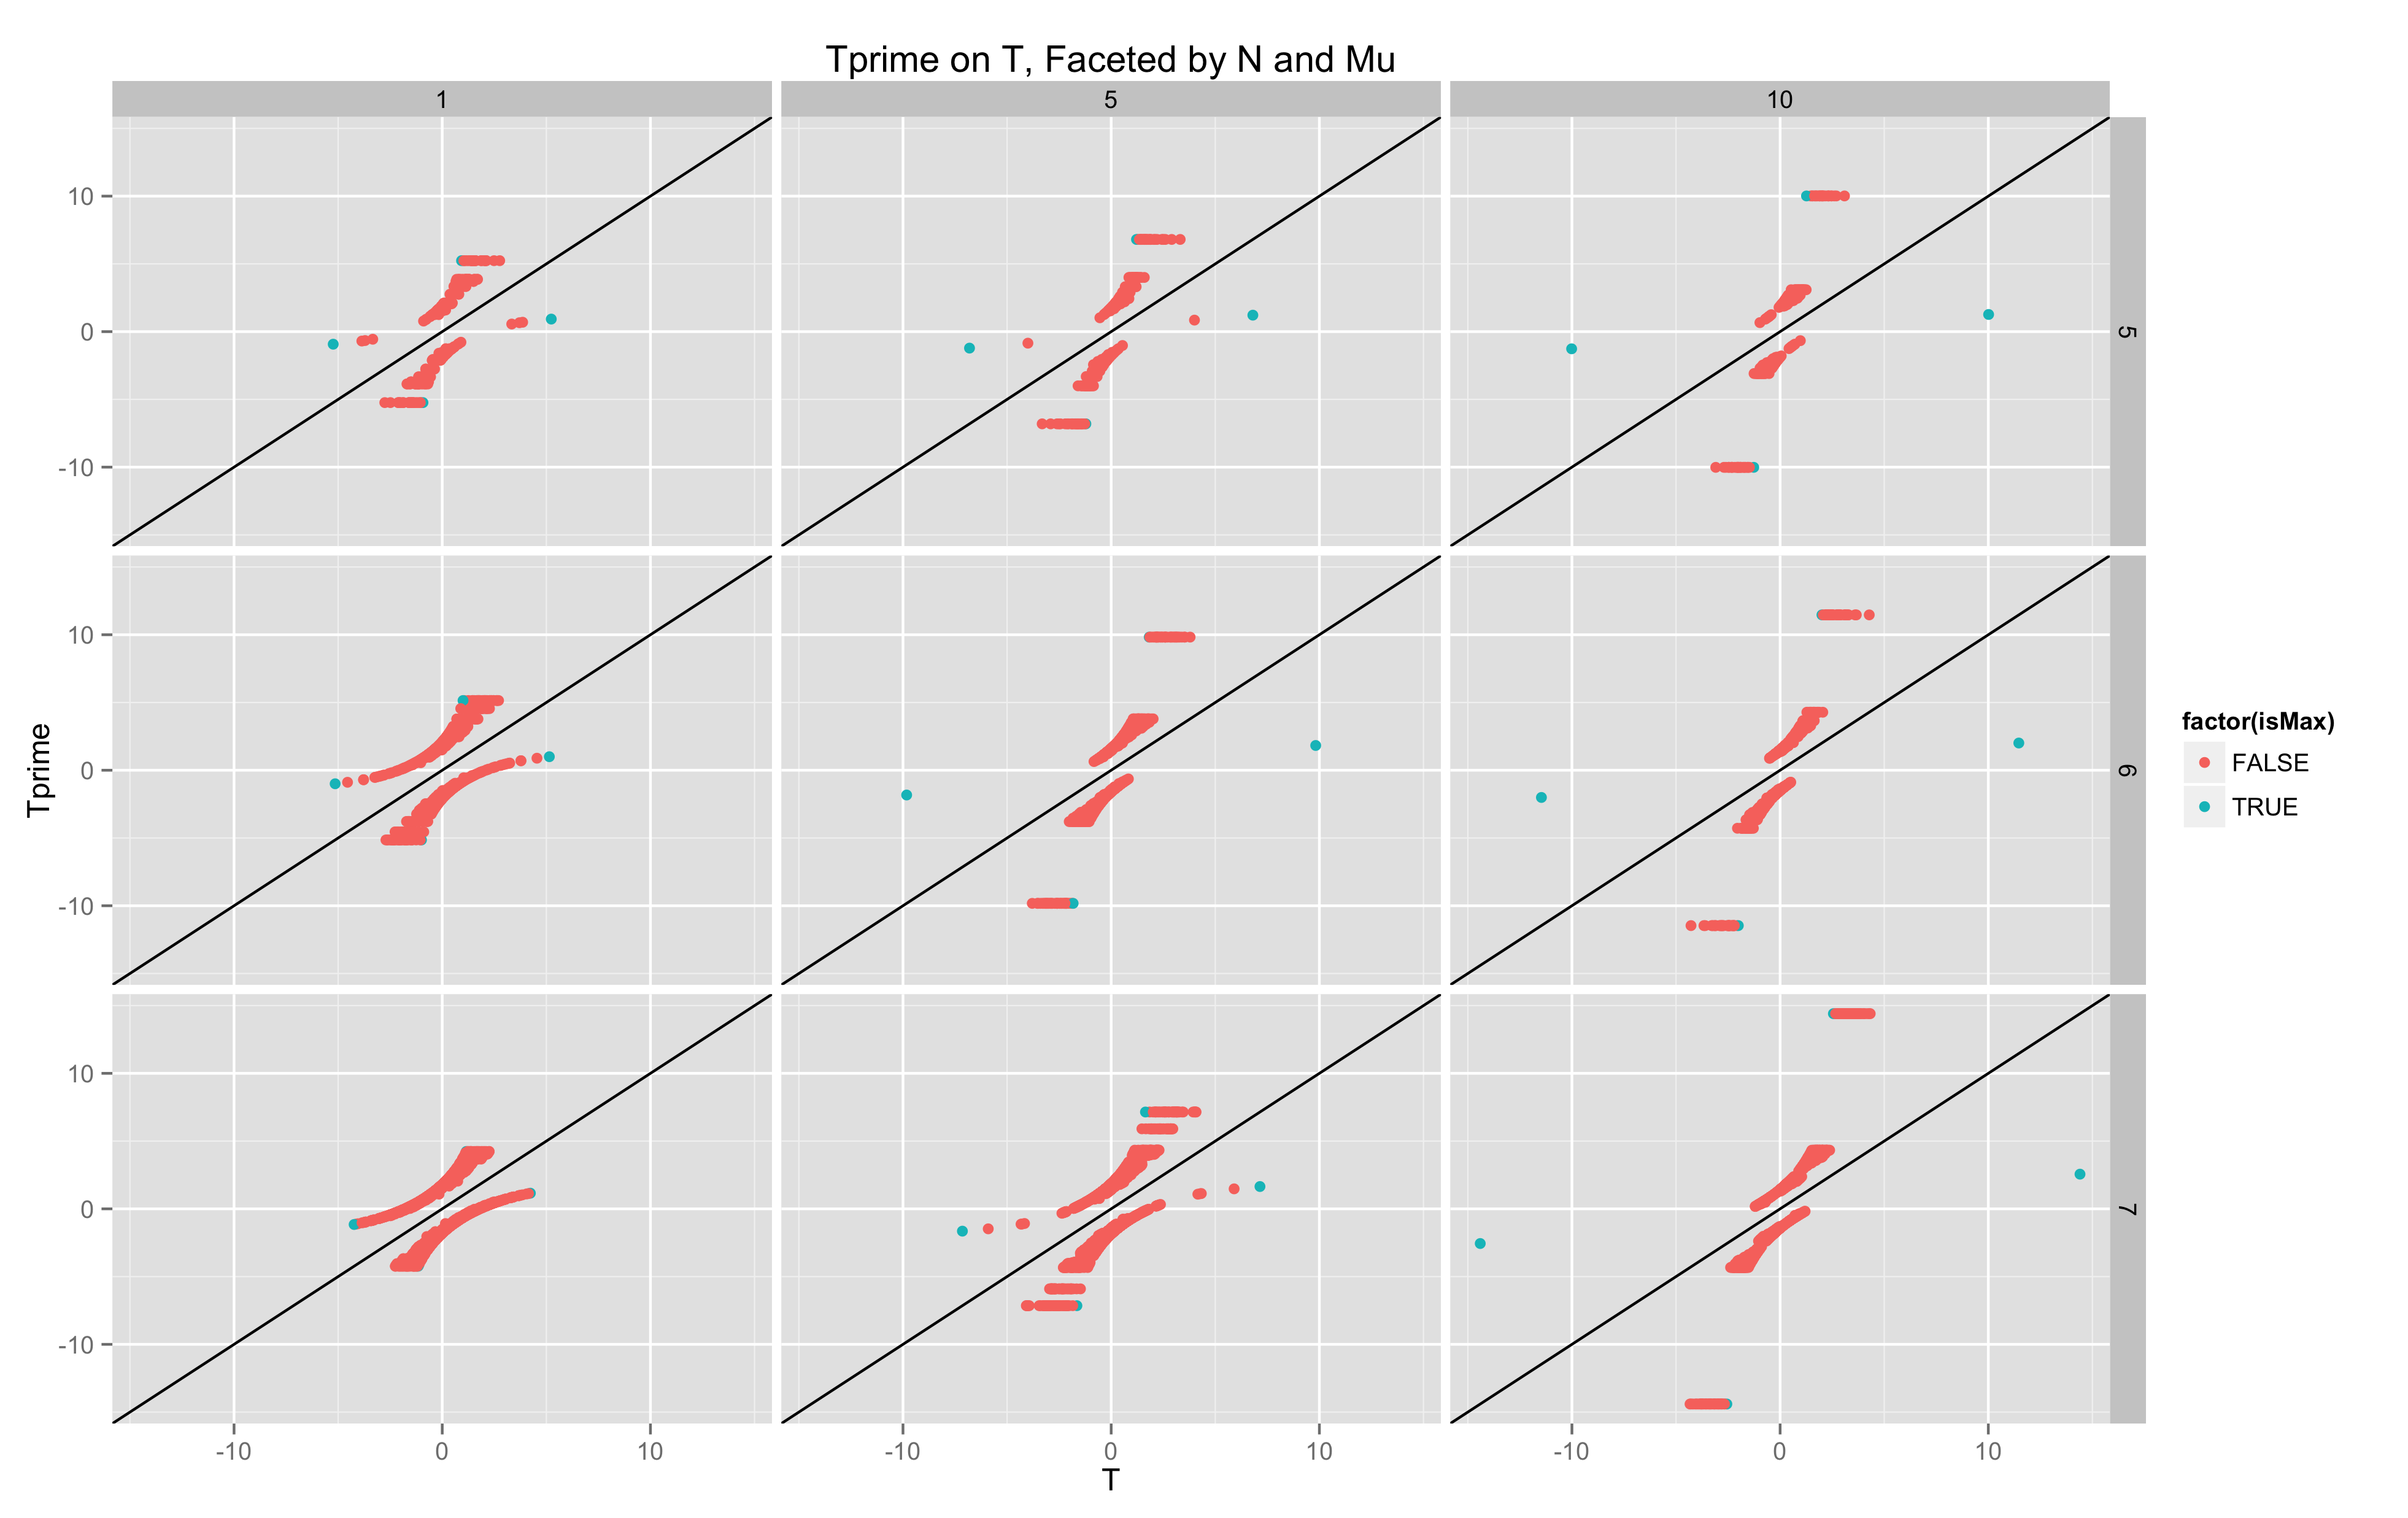
\includegraphics[scale=.12]{./simulations/better_bound_condition/t_tprime_plot.png}
\end{figure}

Unfortunately, we can't make $N$ much bigger than 7 using the current
technique.
\clearpage

\section{Shortcut}
It always seems to be the case that, say, the minimum (equivalently,
the maximum due to symmetry) value of $T_{\pi}$ maximizes $|T - T'|$.
Knowing the permutation $\pi$ that maximizes $|T - T'|$, we can try to
figure out the corresponding transposition $(i, j)$.

It seems reasonable that sorting the data into its order statistics
$\{u_{(i)}\}_{i=1}^{2N}$ will minimize $T$.  That is, let the $N$
smallest be in the first group and the next $N$ in the second.

Another thing that seems reasonable to find the $(i, j)$ that maximizes
$|T - T'|$ is to swap the ``most different'' sample of the first group
with that of the second group: $u_{(1)}$ with $u_{(2N)}$.

I tried this shortcut (it only really involves sorting the data) and
compared it with the exact methodology of the above section and found
agreement in all the tested settings.  This lets us really ramp up $N$
in our simulations.

I haven't really tried to prove it yet: it looks challenging.

Consider drawing sample 1 from $\mathcal{N}(2, \sigma^2)$ and sample 2
from $\mathcal{N}(0, \sigma^2)$ where $\sigma = 1$:
\begin{figure}[!ht]
  \centering
  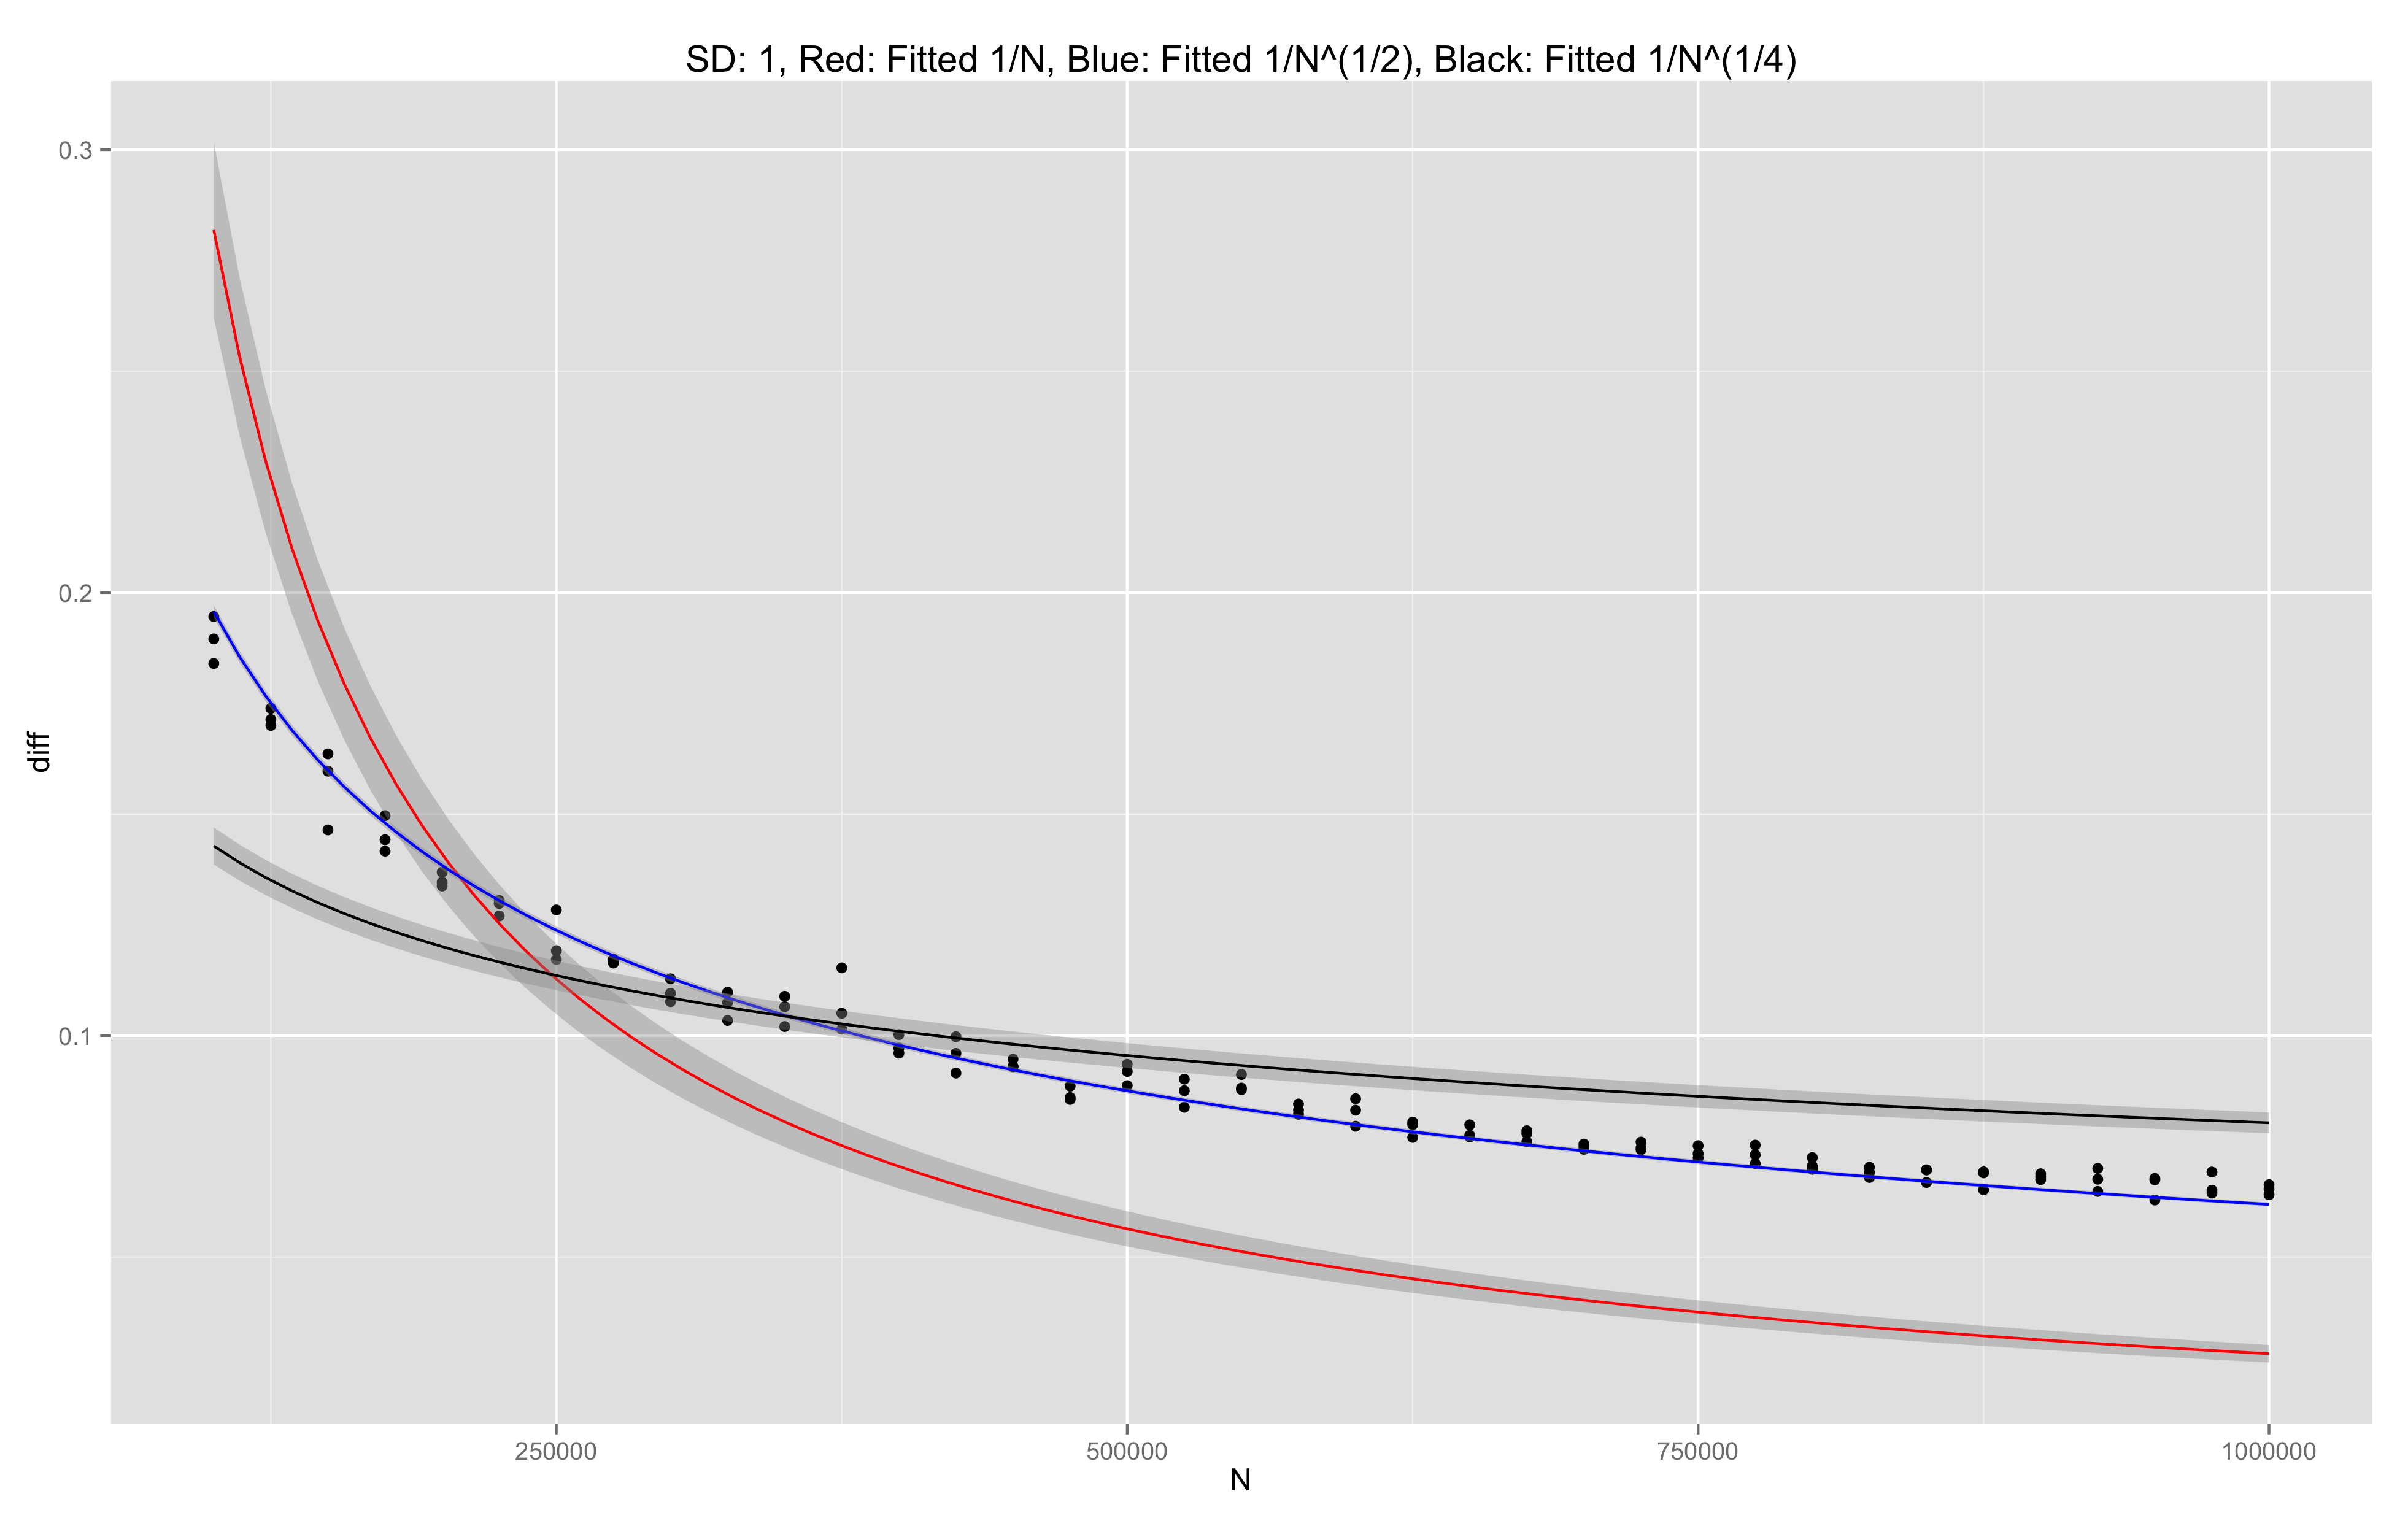
\includegraphics[scale=.06]{./simulations/better_bound_condition/rate_plot_1.png}
\end{figure}

Now consider $\sigma = \sqrt{N}$ (so the power is constant in the
sample size):
\begin{figure}[!ht]
  \centering
  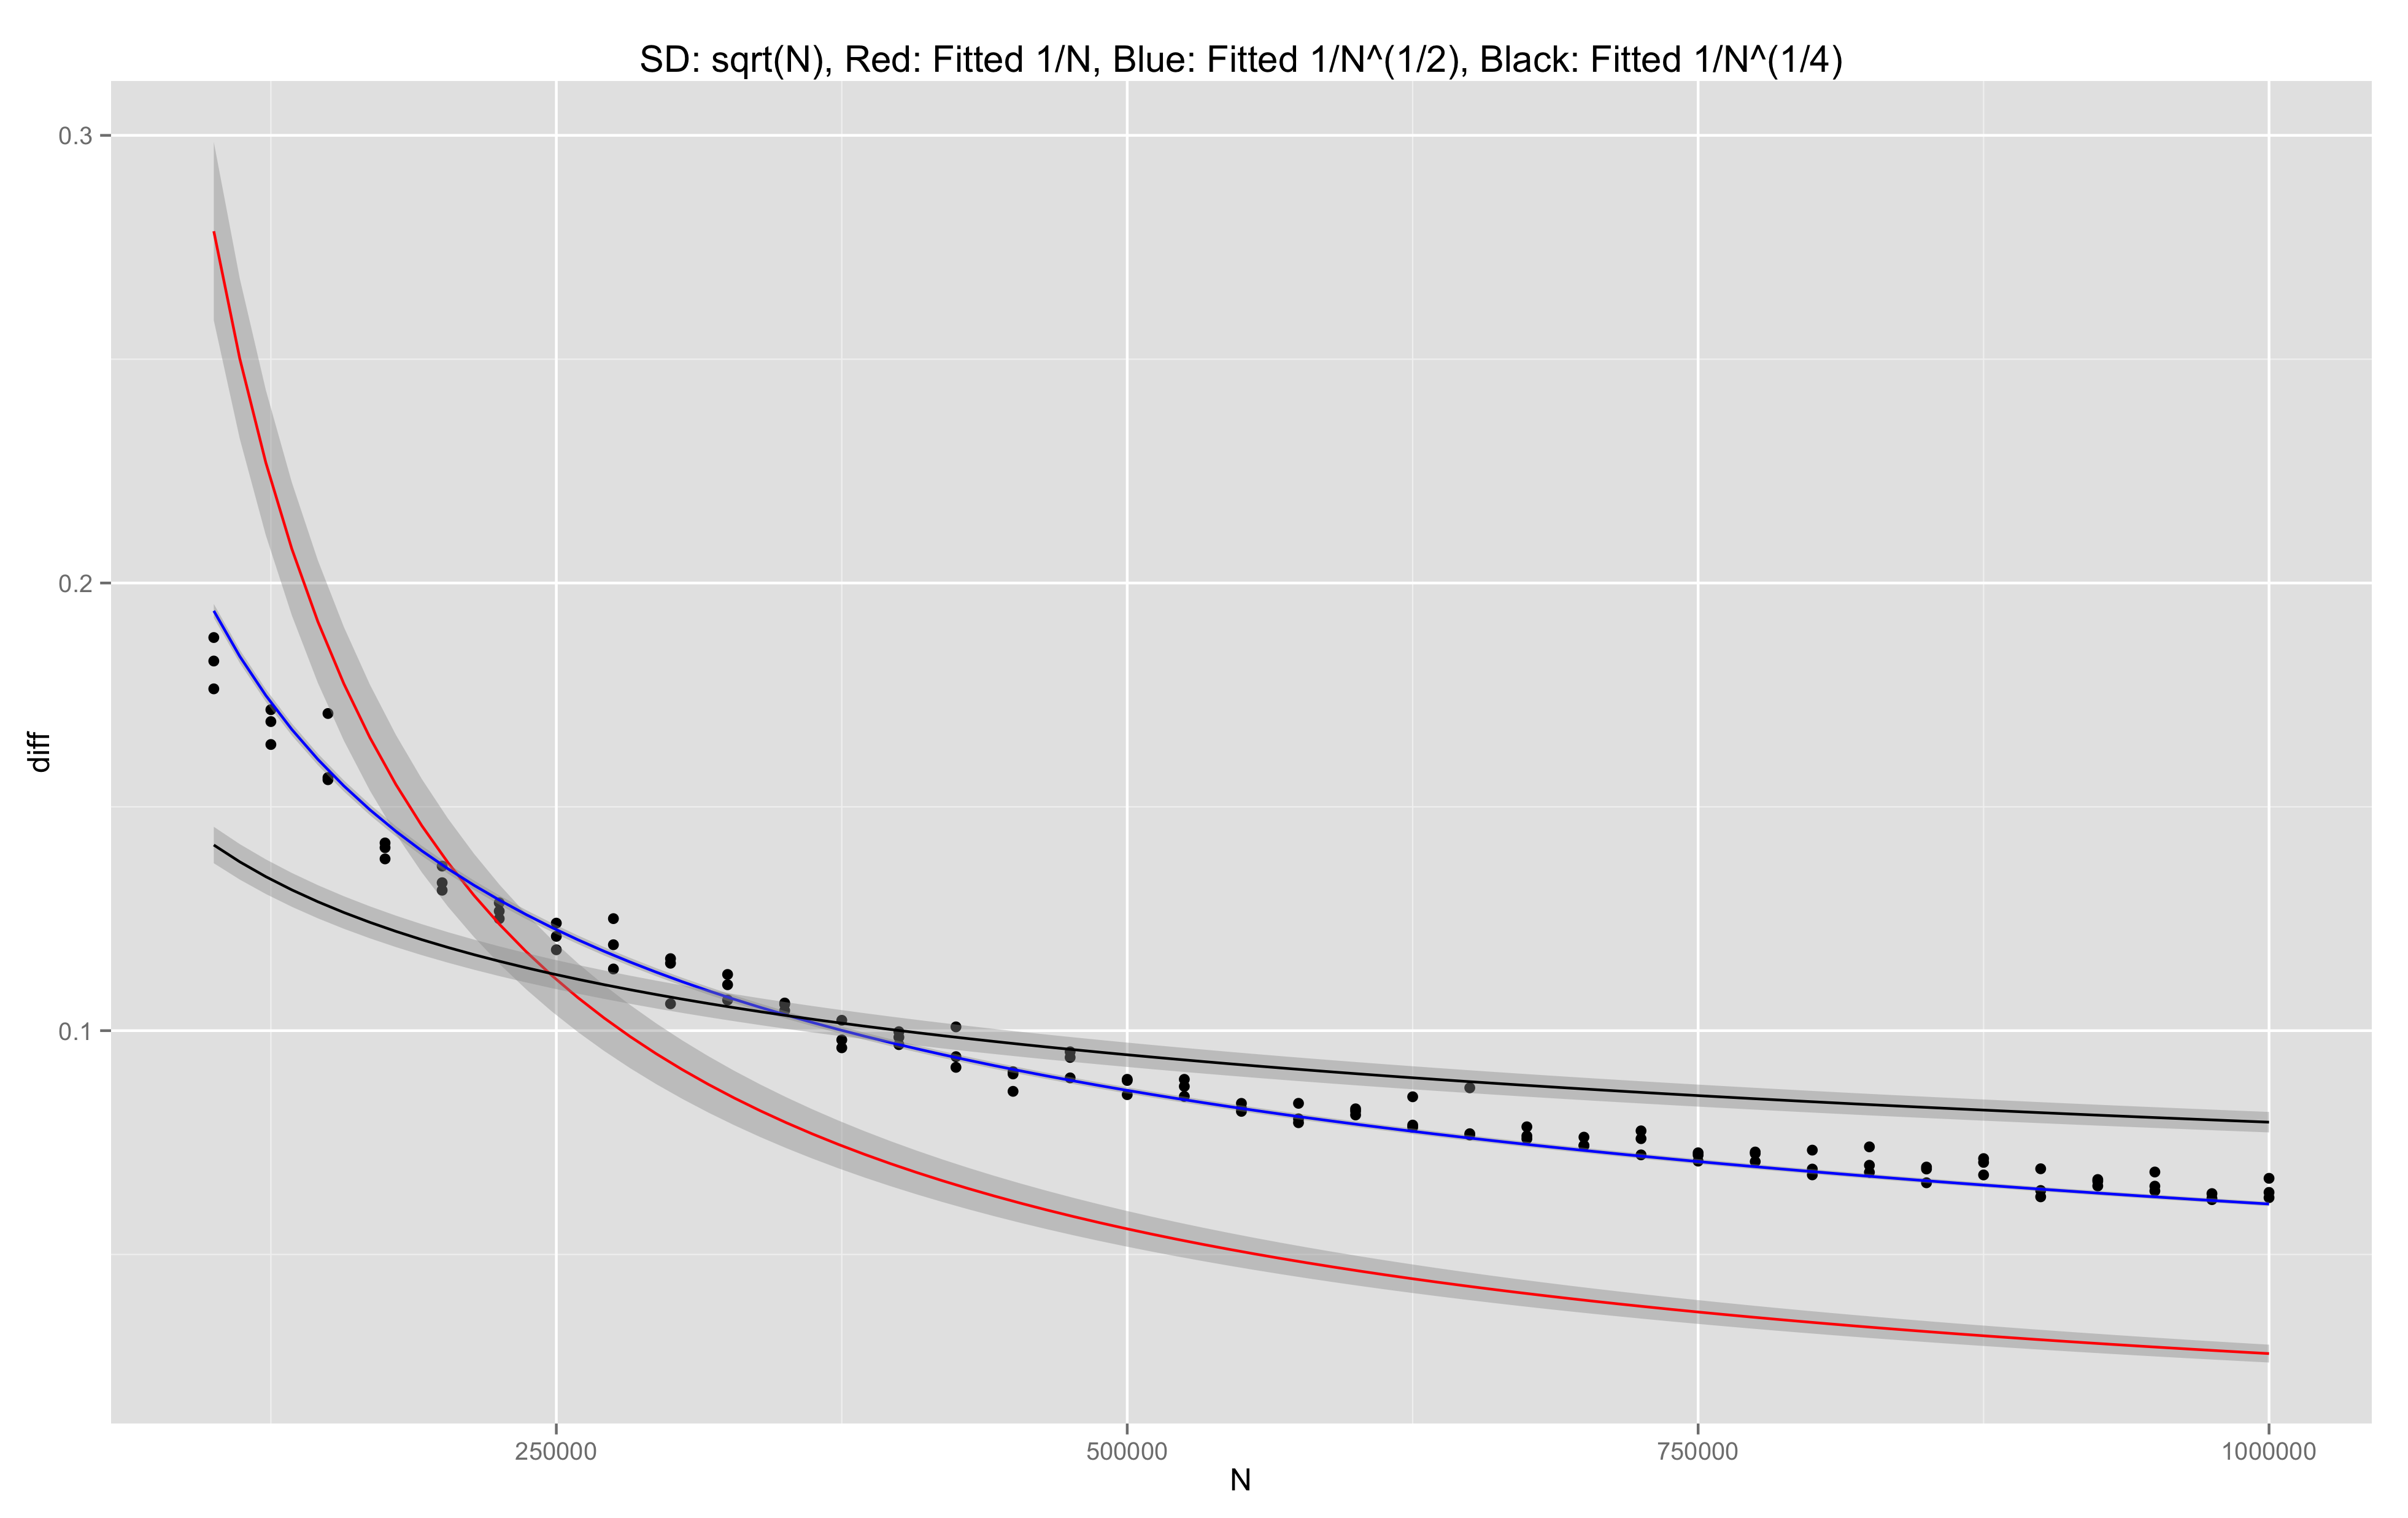
\includegraphics[scale=.06]{./simulations/better_bound_condition/rate_plot_2.png}
\end{figure}

Finally, $\sigma = \frac{1}{\sqrt{N}}$:
\begin{figure}[!ht]
  \centering
  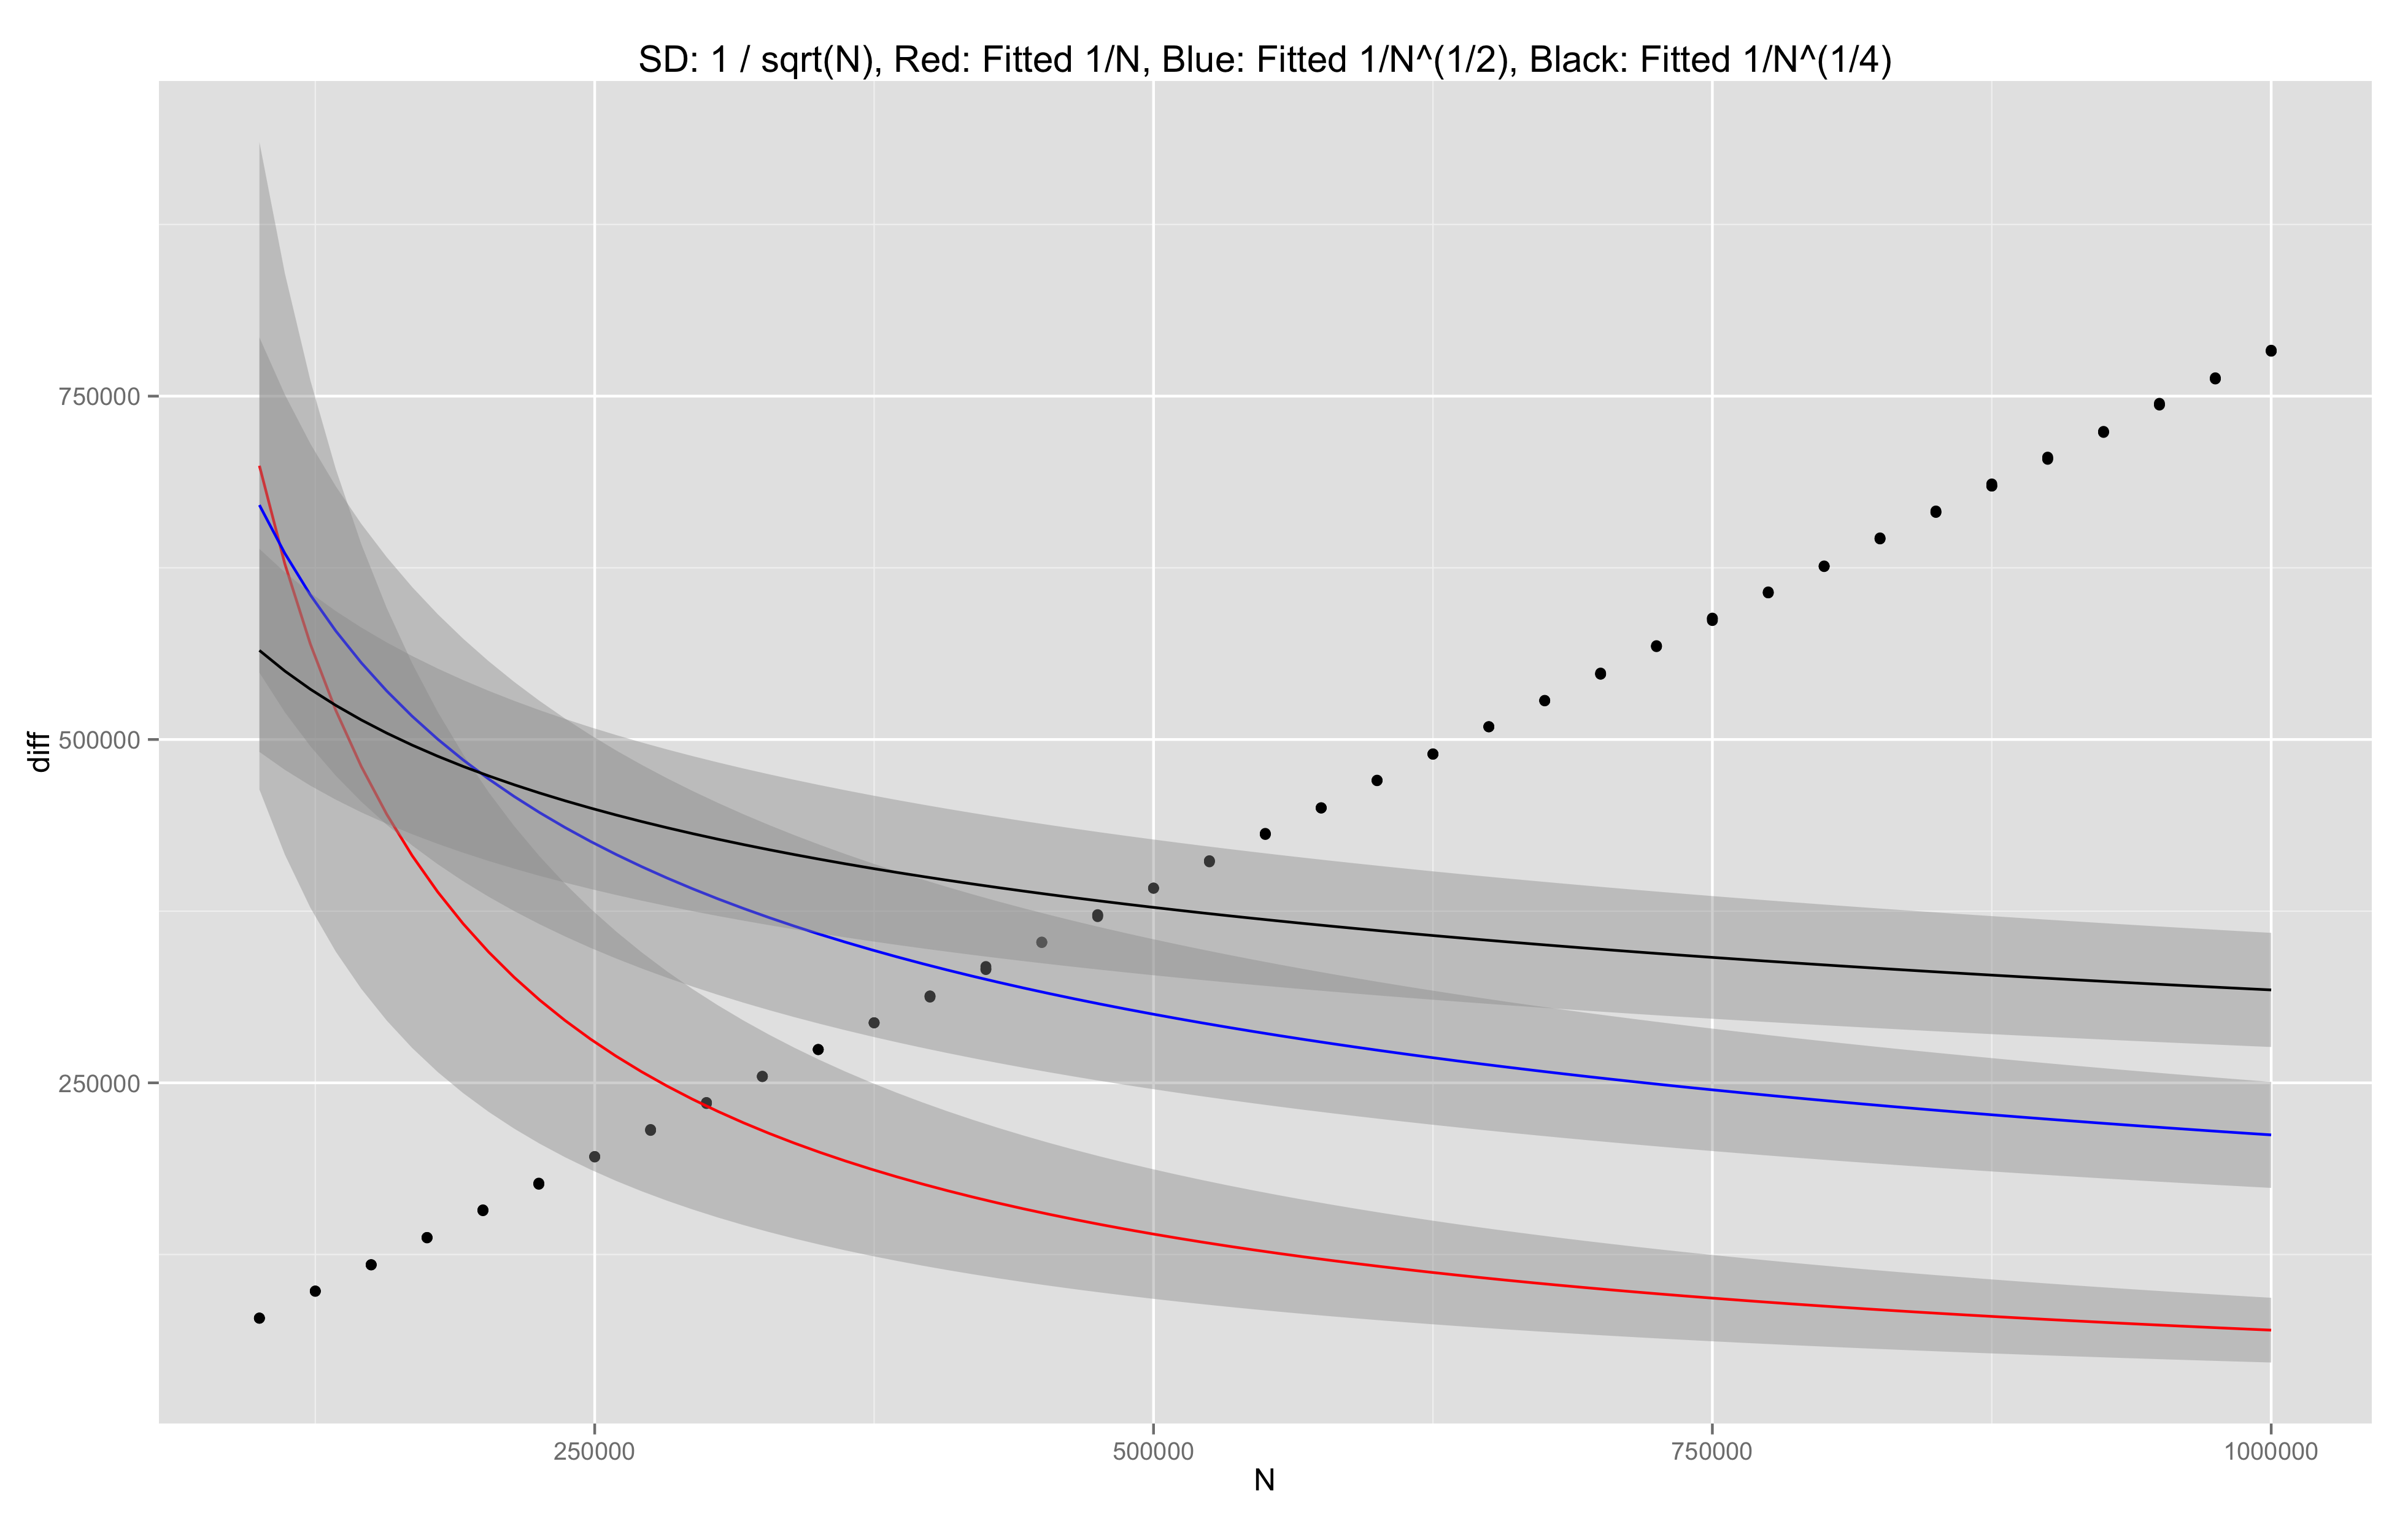
\includegraphics[scale=.06]{./simulations/better_bound_condition/rate_plot_3.png}
\end{figure}

The last situation is one of those pathological cases that we were
trying to avoid, where the within-group variance vanishes so the
distributions tend toward point masses.  But the other reasonable
cases look good.  That is, if the shortcut works, it appears that
$\delta = \max_{\pi, i, j} |T_{\pi} - T_{\pi \circ (i, j)}|$ is
$O(N^{-1/2})$ for these reasonable cases.
